% This one will format for two-sided binding (ie left and right pages have mirror margins; blank pages inserted where needed):
%\documentclass[a4paper,twoside]{ociamthesis}
% This one will format for one-sided binding (ie left margin > right margin; no extra blank pages):
\documentclass[a4paper]{ociamthesis}
% This one will format for PDF output (ie equal margins, no extra blank pages):
%\documentclass[a4paper,nobind]{ociamthesis} 

% !TEX root = ../main.tex

%%%%% SELECT YOUR DRAFT OPTIONS
% Three options going on here; use in any combination.  But remember to turn the first two off before
% generating a PDF to send to the printer!
% This highlights (in blue) corrections marked with (for words) \mccorrect{blah} or (for whole
% paragraphs) \begin{mccorrection} . . . \end{mccorrection}.  This can be useful for sending a PDF of
% your corrected thesis to your examiners for review.  Turn it off, and the blue disappears.
\correctionstrue

%%%%% BIBLIOGRAPHY SETUP
\usepackage{natbib}
\bibliographystyle{plainnat}
% This makes the bibliography left-aligned (not 'justified') and slightly smaller font.
\renewcommand*{\bibfont}{\small}

%%%%% THESIS / TITLE PAGE INFORMATION
% Everybody needs to complete the following:
\title{Automating Inference, Learning, and Design}
\author{Tom Rainforth}
\college{Wolfson College}

% Your full degree name.  (But remember that DPhils aren't "in" anything.  They're just DPhils.)
\degree{Doctor of Philosophy}
% Term and year of submission, or date if your board requires (eg most masters)
\degreedate{Trinity 2017}

\usepackage{microtype}

% use Times
\usepackage{times}
% For figures
\usepackage{graphicx} % more modern
%\usepackage{epsfig} % less modern
%\usepackage{subfigure} 
\usepackage{subcaption} 
\graphicspath{{./part/ipmcmc/figures/}{./misc/figures/}{./bopp/figures/}{./opt/figures/}{./design/figures/}{./nest/figures/}{./inf/figures/}{./part/figures/}{./bayes/figures/}}
\usepackage{tikz}
\usetikzlibrary{fit}					% fitting shapes to coordinates
\usetikzlibrary{backgrounds}	% drawing the background after the foreground
\usepackage{setspace}

\usepackage{cancel}

%\usepackage{svg}

% For algorithms


% For math
\usepackage{amsthm}
\usepackage{dsfont}
\usepackage{amssymb,amsmath}
\usepackage{bbm}

%\newcommand{\theHalgorithm}{\arabic{algorithm}}

\usepackage{hyperref}

\usepackage{bibentry}
\nobibliography*


% % BOPP

%\usepackage{enumitem}
%\setlist[itemize]{leftmargin=*}
%\usepackage{paralist}
\usepackage{footmisc}
\usepackage{listings}
\usepackage{color}
\usepackage{xcolor}
\usepackage{textcomp}
\usepackage{xspace}
\usepackage{amsbsy}
\usepackage{siunitx}
%\usepackage{algorithmicx}
%\usepackage{algpseudocode}
\usepackage{mathtools}
\usepackage{array}
\usepackage{booktabs}
\usepackage{adjustbox}
\usepackage{microtype}
\usepackage{todonotes}

\usepackage{wrapfig}
\usepackage{thmtools}
\usepackage{thm-restate}

\newcommand{\angurl}{\scriptsize \url{http://www.robots.ox.ac.uk/~fwood/anglican}}
\newcommand{\myurl}{\scriptsize \url{https://bitbucket.org/twgr/ipmcmc}}

%\definecolor{darkgreen}{rgb}{0.25,.5,0}
%\definecolor{blue}{rgb}{0,0.33,0.66}
%\definecolor{red}{rgb}{0.66,0.0,0.0}
%\definecolor{purple}{rgb}{0.33,0,0.66}
%\definecolor{cyan}{rgb}{0.0,0.5,0.5}
%\definecolor{orange}{rgb}{0.5,0.25,0.0}
%\definecolor{gray}{rgb}{0.4,0.4,0.4}
\lstset{ 
	language=Lisp, 
	basicstyle=\small\ttfamily,
	keywordstyle={}, 
	alsoletter={/},
	alsoletter={:},
	alsoletter={*},
	alsoletter={<-},
	commentstyle=\em \color{gray}, 
	frame=lines,
	%float=tbph,
	% captionpos=b,
	showstringspaces=false, 
	keywordstyle=[1]\bf\ttfamily\color{blue},
	keywords=[1]{BO,theta-best,bo-acquire,sample-initial-points,sample,observe,observe*,observe<-,predict,store,retrieve,return,catch,throw},
	keywordstyle=[2]\bf\ttfamily\color{red},
	keywords=[2]{defn,if,let,letfn,loop,looppredict,recur},
	keywordstyle=[3]\bf\ttfamily\color{cyan},
	keywords=[3]{absorb,assoc,argmax,count,cons,conj,dirichlet-discrete,do,exponential,first,flip,fn,gamma,beta,get,keys,lazy-seq,map,mvn-niw,nth,mat/add,mat/div,normal,print,produce,reduce,repeat,repeatedly,rest,set,shape,take,uniform-continuous,vec,distribution,factor,simulate,abc-likelihood,when,max},
	keywordstyle=[4]\bf\ttfamily\color{purple},
	keywords=[4]{defopt,defquery,doopt,doquery,query,defdist},
	keywordstyle=[5]\ttfamily\color{orange},
	keywords=[5]{:nu,:alpha,:id},
	mathescape=true,
	stringstyle={},
} 
\lstnewenvironment{code}[2]{\lstset{caption=#1,label=#2}}{}

\newtheorem{example}{Example} 
\newtheorem{theorem}{Theorem}[chapter]
\newtheorem{lemma}[theorem]{Lemma} 
%\newtheorem{proposition}[proposition]{Proposition} 
\newtheorem{remark}{Remark}
%\newtheorem{corollary}[corollary]{Corollary}
\newtheorem{definition}{Definition}[chapter]
%\newtheorem{conjecture}[conjecture]{Conjecture}
%\newtheorem{axiom}[axiom]{Axiom}

% % % % % % % % % % % % % % % % % % %


\usepackage{packages/naesseth}
%\usepackage{packages/algorithm,packages/algorithmic}
\usepackage{packages/abbreviations}

\usepackage{algorithmicx}
\usepackage{algorithm}
\usepackage{algpseudocode}
\usepackage{setspace}
% % % % % % % % %
\algnewcommand\algorithmicswitch{\textbf{switch}}
\algnewcommand\algorithmiccase{\textbf{case}}
\algnewcommand\algorithmicassert{\texttt{assert}}
\algnewcommand\Assert[1]{\State \algorithmicassert(#1)}%
% New "environments"
\algdef{SE}[SWITCH]{Switch}{EndSwitch}[1]{\algorithmicswitch\ #1\ \algorithmicdo}{\algorithmicend\ \algorithmicswitch}%
\algdef{SE}[CASE]{Case}{EndCase}[1]{\algorithmiccase\ #1}{\algorithmicend\ \algorithmiccase}%
%\algtext*{EndSwitch}%
\algtext*{EndCase}%

%\ShortHeadings{Automating Inference, Learning, and Design}{Tom Rainforth}
%\firstpageno{1}

\begin{document} 

%%%%% CHOOSE YOUR LINE SPACING HERE
% This is the official option.  Use it for your submission copy and library copy:
%\setlength{\textbaselineskip}{22pt plus2pt}
\setlength{\textbaselineskip}{22pt plus2pt minus1pt}
% This is closer spacing (about 1.5-spaced) that you might prefer for your personal copies:
%\setlength{\textbaselineskip}{18pt plus2pt minus1pt}

% You can set the spacing here for the roman-numbered pages (acknowledgements, table of contents, etc.)
\setlength{\frontmatterbaselineskip}{17pt plus1pt minus1pt}

% Leave this line alone; it gets things started for the real document.
\setlength{\baselineskip}{\textbaselineskip}


%%%%% CHOOSE YOUR SECTION NUMBERING DEPTH HERE
% You have two choices.  First, how far down are sections numbered?  (Below that, they're named but
% don't get numbers.)  Second, what level of section appears in the table of contents?  These don't have
% to match: you can have numbered sections that don't show up in the ToC, or unnumbered sections that
% do.  Throughout, 0 = chapter; 1 = section; 2 = subsection; 3 = subsubsection, 4 = paragraph...

% The level that gets a number:
\setcounter{secnumdepth}{3}
% The level that shows up in the ToC:
\setcounter{tocdepth}{2}

% JEM: Pages are roman numbered from here, though page numbers are invisible until ToC.  This is in
% keeping with most typesetting conventions.
\begin{romanpages}
	
	% Title page is created here
	\maketitle
	
	%%%%% DEDICATION -- If you'd like one, un-comment the following.
	%\begin{dedication}
	%This thesis is dedicated to\\
	%someone\\
	%for some special reason\\
	%\end{dedication}
	
	%%%%% ACKNOWLEDGEMENTS -- Nothing to do here except comment out if you don't want it.
	\begin{acknowledgements}
		% !TEX root = ../main.tex

\vspace{20pt}
I would first like to thank by partner Sophie for her support and understanding through this
process and for all the sacrifices she has made on my behalf.  I would similarly like to
thank my family for their unwavering support and making me who I am today.  I would like
to thank Frank Wood, Jan-Willem van de Meent, and Brooks Paige for their guidance and
support, both academic and personal.  I owe them all, particularly Frank and Jan-Willem,
a huge debt of gratitude for teaching me most of what I know, nurturing me from an
arrogant fool who asked questions like \emph{Metropolis what?} to an even more arrogant
fool who thinks he knows everything.  This work would have been a terrible failure without them.
I would like to thank my friends and colleagues 
Atılım Güneş Baydin, Rob Cornish, Piotr Czaban, Neil Dhir, Jack Fitzsimons, Adam Goliński,
Bradley Gram-Hansen, Max Igl, David Janz, Tom Jin, Tuan Anh Le, Mario Lezcano, 
Aravindh Mahendran, David Martínez Rubio, Siddharth N, Nantas Nardelli, Michael Osborne,
Nick Palmius, Yura Perov, David Tolpin, Andrea Vedaldi, Andrew Warrington, Stefan Webb, 
Hongseok Yang, Yuan Zhou, and Rob Zinkov, for making this time in Oxford some of the 
happiest of my life.  I would like to thank my previously unmentioned coauthors Arnaud Doucet, Fredrik Lindsten,
Christian A. Naesseth, and Benjamin Vincent, for being an absolute pleasure to work with.
Finally, I would like to thank BP for providing the funding for this research.

Much of the novel material in this thesis is from coauthored work and it would be fabrication
to claim it all as my own.  In particular, a lot of the work is based around the probabilistic 
programming system \emph{Anglican}, for which all the credit must go to Frank Wood,
Jan-Willem van de Meent, and David Tolpin. Elsewhere, citations are made
to the original coauthored papers upon which this work is based, for which credit
must go to all my coauthors.
	\end{acknowledgements}
	
	%%%%% ABSTRACT -- Nothing to do here except comment out if you don't want it.
	\begin{abstract}
		% !TEX root = ../main.tex

\vspace{20pt}
Imagine a world where computational simulations can be inverted as easily as running them forwards, where data
can be used to refine models automatically, and where the only expertise one needs to carry
out powerful statistical analysis is a basic proficiency in scientific coding.  Creating such a
world is the ambitious long-term aim of \emph{probabilistic programming}.

The bottleneck for improving the probabilistic models, or simulators, used throughout the quantitative sciences,
is often not an ability to devise better models conceptually,  but a lack of expertise,
time, or resources to realize such innovations.
Probabilistic programming systems (PPSs) help alleviate this bottleneck 
by providing an expressive and accessible modeling framework,
%, often more in line we conventional scientific simulation than mainstream statistical approaches,
 then
automating the required computation to draw inferences from the model, for example finding
the model parameters likely to give rise to a certain output.
By decoupling model specification and inference, PPSs 
streamline the process of developing and drawing inferences from new models, while
opening up powerful statistical methods to non-experts.
%open up powerful statistical methods 
%to non-experts, while
%streamlining the process of developing new models or inference algorithms
%those within the machine learning and statistics communities.  
Many systems further provide
the flexibility to write new and exciting models which would be hard, or even impossible, to convey using 
conventional statistical frameworks.

The central goal of this thesis is to improve and extend PPSs.
%, providing some of the many steps
%that will be necessary to achieve the lofty long-term aims of the field.  
In particular, we will
make advancements to the underlying inference engines and increase the
range of problems which can be tackled.  For example, we will extend PPSs to a mixed inference-optimization
framework, thereby providing automation of tasks
such as model learning and engineering design.  Meanwhile, we make inroads into constructing systems
for automating adaptive sequential design problems, providing potential applications across the sciences.
Furthermore, the contributions of the work reach far beyond probabilistic programming, as 
achieving our goal will require us to make
advancements in a number of related fields such as particle Markov chain Monte Carlo methods,
Bayesian optimization, and Monte Carlo fundamentals. %, and Bayesian experimental design.

%
%Specifically, we will introduce \emph{interacting particle
%	Markov chain Monte Carlo},
%a new inference algorithm suitable for large-scale computation, and 
%detail is implementation as a general purpose inference engine for the PPS \emph{Anglican}. 
%%explain how it can be
%%used as general purpose inference engine for PPSs by detailing its implementation
%%in the PPS \emph{Anglican}.  
%We will extend PPSs beyond their typical inference setting
%to a more general mixed inference-optimization framework by introducing~\emph{Bayesian
%	optimization for probabilistic programs}, thereby providing automation of tasks
%such as model learning and engineering design.
%%in the same manner as inference is automated in existing systems.  
%We will develop theoretical 
%results on \emph{nesting Monte Carlo
%	estimators} and explain the important implications these have for nesting models in PPSs.
%Finally, we will 
%%examine a particular
%%class of nested estimation problems, those of Bayesian experimental design, and 
%introduce a high-level framework for automating adaptive sequential design problems, 
%%a particle example 
%providing application of our technique to psychological trials.
%%Finally, we will examine a particular
%%class of nested estimation problems, those of Bayesian experimental design, and introduce
%%a high-level framework for automating arbitrary adaptive sequential design problems,
%%providing application our technique to psychological trials.
	\end{abstract}
	
	%%%%% MINI TABLES
	% This lays the groundwork for per-chapter, mini tables of contents.  Comment the following line
	% (and remove \minitoc from the chapter files) if you don't want this.  Un-comment either of the
	% next two lines if you want a per-chapter list of figures or tables.
	\dominitoc % include a mini table of contents
	%\dominilof  % include a mini list of figures
	%\dominilot  % include a mini list of tables
	
	% This aligns the bottom of the text of each page.  It generally makes things look better.
	\flushbottom
	
	% This is where the whole-document ToC appears:
	\tableofcontents
	
	%\listoffigures
	\mtcaddchapter
	% \mtcaddchapter is needed when adding a non-chapter (but chapter-like) entity to avoid confusing minitoc
	
	% Uncomment to generate a list of tables:
	%\listoftables
	%	\mtcaddchapter
	
	%%%%% LIST OF ABBREVIATIONS
	% This example includes a list of abbreviations.  Look at text/abbreviations.tex to see how that file is
	% formatted.  The template can handle any kind of list though, so this might be a good place for a
	% glossary, etc.
	% !TEX root = ../main.tex

% First parameter can be changed eg to "Glossary" or something.
% Second parameter is the max length of bold terms.
\begin{mclistof}{Glossary and Abbreviations}{3.2cm}

\item[\smc] Sequential Monte Carlo.  A general purpose inference method using a series of 
intermediary targets.

\end{mclistof} 

	
	% The Roman pages, like the Roman Empire, must come to its inevitable close.
\end{romanpages}

\setlength{\abovedisplayskip}{6.5pt}
\setlength{\belowdisplayskip}{6.5pt}
\setlength{\abovedisplayshortskip}{6.5pt}
\setlength{\belowdisplayshortskip}{6.5pt}
\renewcommand{\chapterheadstartvskip}{\vspace*{-80pt}}

% !TEX root = ../main.tex

\chapter{Introduction}
\label{chp:intro}

% !TEX root = ../main.tex

How come a dog is able to catch a
frisbee in mid-air? How come a batsman can instinctively predict the flight of a cricket ball
moving at over $100$km/h sufficiently accurately and quickly to hit it with the bat when there
is not even time to consciously make a prediction?  Clearly, neither can be based on a
deep explicit knowledge of the laws of physics or some hard-coded model for the movement
of objects; we are not even born with the knowledge that unsupported objects will 
fall down~\citep{baillargeon2002acquisition}.  The only reasonable explanation for these
abilities is that the batsmen and the dog have \emph{learned from experience}.  We do not have
all the knowledge we require to survive from birth, but we are born with the
ability to learn and adapt, making observations about the world around us and using these
to refine our cognitive models for everything from the laws of physics to social interaction.
Classically the scientific method has relied on human interpretation of the world to formulate
explicit models to explain our internal intuitions, which we then test
through experimentation.  However, even as a whole scientific society, our models
are often terribly inferior to the subconscious models of animals and children, such as for most
tasks revolving around social interaction.  This leads one to ask, is there something fundamentally
wrong with this hand-crafted modeling approach?  Is there another approach that better mimics the
way humans themselves learn?

\emph{Machine learning} is an appealing alternative, and often complementary,
approach that focuses on constructing algorithms and systems that can adapt, or learn, from data in order
to make predictions that have not been explicitly programmed.
This is exciting not only because of the potential it brings
to automate and improve a wide array of computational tasks, but because it allows us to design 
systems capable of going beyond the boundaries of human understanding, reasoning
about and making predictions for tasks we cannot solve directly ourselves.
As a field, machine learning is very wide ranging,
straddling computer science, statistics, engineering, and beyond. 
It is perhaps most closely related to the field of computational statistics, differing predominantly
in its emphasis on prediction rather than understanding.  Despite the current hype around the
field, most of the core ideas have existed for some
time, often under the guise of pattern recognition, artificial intelligence, or computational 
statistics.  Nonetheless, the explosion in the availability of data and in computational processing power in recent
years has led to a surge of interest in machine learning by academia and industry alike, particularly 
in its application to real world problems.  This interest alone is enough to forgive the hype as the
spotlight is not only driving the machine learning community itself forward, but helping identify
huge numbers of applications where existing techniques can be transferred to fantastic effect.
From autonomous vehicles~\citep{lefevre2014survey}, to speech recognition \citep{jurafsky2014speech},
and designing new drugs \citep{burbidge2001drug}, machine learning is rapidly becoming a 
crucial component in many technological and scientific advancements.  

%From autonomous vehicles~\citep{lefevre2014survey}, to speech recognition \citep{jurafsky2014speech},
%and designing new drugs \citep{burbidge2001drug}, machine learning is rapidly becoming a 
%crucial component in many technological and scientific advancements.  
%At its heart, it is the study of algorithms which can adapt, or learn, from data in order
%to make predictions that have not been explicitly programmed by the user.  It is a wide ranging field,
%straddling computer science, statistics, engineering, and beyond. Though it has existed for some
%time, often under the guise of pattern recognition, artificial intelligence, or computational 
%statistics, the explosion in the availability of data and in computational processing power in recent
%years has led to a surge of interest in machine learning by academia and industry alike, particularly 
%in its application to real world problems.  This is exciting not only because of the potential it brings
%to automate and improve a wide array of computational tasks, but because it allows us to design 
%systems capable of going beyond the boundaries of human understanding and prediction, reasoning
%about and making predictions for tasks we cannot solve directly ourselves.

In many machine learning applications, it is essential to use a principled \emph{probabilistic} 
approach \cite{ghahramani2015probabilistic}, incorporating uncertainty and utilizing all the information at hand, 
particularly when data is scarce.  The \emph{Bayesian paradigm} provides an excellent basis upon which to do this: an area 
specialist constructs a probabilistic model for data generation, conditions this on the actual observations received, 
and, using Bayes' rule, receives an updated model incorporating this information.  This
allows information from both existing expertise and data to be combined in a statistically
rigorous fashion.  As such, it allows us to use machine learning to complement the conventional
scientific approach, rather than directly replacing it: we can construct models in a similar way to
that which is already done, but then improve and refine these models using data.

Unfortunately, there are two key stumbling blocks that often make it difficult for this idealized
view of the Bayesian machine learning approach to be realized in practice.  Firstly, a process 
known as \emph{Bayesian inference} is
required to solve the specified problems.  This is typically a challenging task, closely 
related to integration, which is often computationally intensive to solve.  Furthermore, it often
requires significant statistical expertise to implement effectively, creating a substantial barrier to
entry.  
Secondly, it can be challenging to specify models that are true to the assumptions the user
wishes to make and the prior information available.  It can again require statistical expertise to abstract
application specific knowledge to a valid statistical model.  Furthermore, assumptions are often made in the interest
of the tractability of inference, rather than the fidelity of the model.  Perhaps because of these drawbacks, there is often
a reliance on off-the-shelf solutions, even when these models are somewhat inappropriate for the task
at hand.

%Similar scenarios of limited data are prevalent through all areas of research; medical trials, materials testing, drug discovery, design of robotic movement and engineering design, to name but a few.  Indeed, the prevalence of such problems is so large, that the problem in solving them is arguably more one of expertise than appropriate techniques.  Bayesian approaches offer a powerful means to mathematically formalize these problems, but the required expertise to effectively solve the resulting inference can be prohibitive, or at least problematic and time consuming, particularly for those from less mathematical backgrounds.

Probabilistic programming systems (PPS) \citep{goodman2008church} are an attempt to
overcome this dichotomy between the Bayesian ideal and common practice.  Their core philosophy 
is to decouple model specification and inference, the former corresponding to the user-specified 
program code, composing of a generative model and statements for conditioning on data, and the 
latter to an inference engine capable of operating on arbitrary programs.  This abstraction barrier 
allows users with domain specific knowledge to write models naturally, as if they were writing a 
simulator, without worrying about the inference, which becomes the job of the developer. Informally 
one can think of PPS as operating as inverse probability engines, outputting the conditional 
probability distribution implied by the generative model coupled with the observed data.
Removing the need for users to worry about the required inference significantly reduces the 
burden of developing new models, and makes effective statistical methods accessible to 
non-experts.  From a developer's perspective, the abstraction can also aid in the design 
and testing of new inference algorithms.  Furthermore, the availability of the target source 
code, with known semantics, opens up many opportunities for new methods that would
not otherwise be possible.

The underlying theme of this thesis is improving and extending probabilistic programs.  However,
doing this will require us to make advancements in a number of different research areas such
as particle Markov chain Monte Carlo methods~\citep{andrieu2010particle,rainforth2016interacting},
Bayesian optimization~\citep{movckus1975bayesian,rainforth2016bayesian}, and \mc
fundamentals~\cite{metropolis1949monte,rainforth2016pitfalls}.  Our aim is to both improve
the performance of PPS by improving the underlying inference engines, increasing
efficiency and the range of models for which inference can be tractably provided for, and to increase
the scope of problems which can be covered by PPS more generally.  In particular, we
will extend PPS beyond the standard Bayesian inference setting to more general frameworks
such as marginal maximum a posteriori estimation and nested estimation.  This opens up a number
of fascinating opportunities, such as the prospect of constructing systems for automating the
design of adaptive experiments and for carrying out principled, probabilistic, engineering simulations
that explicitly incorporate the uncertainty in the task at hand.

\todo[inline]{Build on this a bit so that is a full motivation section.  In particular, could do a better
	job of linking it back to the real world.  Could also do more of a linking of my work to the aims, 
	rather than just probabilistic programming in general.}

\section{Thesis Aims and Layout}

This thesis contains a mixture of pedagogical material, literature review, and 
cutting-edge research.
Although there will inevitably be gaps, the aim is to take
the reader all the way from the fundamentals of probability and machine learning,
all the way through to highly advanced topics such as designing automatic
mixed inference-optimization engines for probabilistic programming languages,
such that the work is as self-contained as is realistically possible.  There are
three key rationales for doing this.  Firstly, it is done because our aim to make the work 
as accessible as possible and hopefully provide a useful guide to those new to the field.
Probabilistic programming, and machine learning more generally, draws
researchers from an exceptionally diverse pool of backgrounds; what is rudimentary
to, for example, the statistics community is often bewildering to the programming
languages community and vice-versa. Secondly, because probabilistic programing, and 
in particular the advanced content of this thesis, goes beyond conventional notions of
Bayesian modeling, 

Thirdly, we take a predominantly first principles approach because it is the authors' 
opinion that because machine learning moves so quickly, or perhaps simply because
of the nature of research itself, one tends to become so fixated on a small area of
research that the big picture becomes lost.  For good research it is important to not
only question ones contribution to a particular sub-field, but also the justification for
that subfield itself.  With the current hype surrounding machine learning and, in particular,
deep learning\footnote{Should be pronounced \emph{neu-ral net-works}}, returning to these
fundamental principles is more important than ever so that we know what the right approach
for a particular problem is.
% !TEX root = ../main.tex

\chapter{A Brief Introduction to Probability Theory}
\label{chp:prob}

Before going into the main content of the paper, we first provide a quick primer on probability
theory, providing some essential background and outlining conventions
that we will use throughout the thesis.  Readers familiar with the differences between a probability
and a probability density and between a random variable and an outcome may wish skip to this
Chapter, referring back as needed for clarification on any conventions undertaken.  Others
will hopefully find it to be a gentle introduction to the key concepts that will be needed to
be understood to follow the rest of the thesis.  Notation has been chosen with accessibility 
as the primary aim and we will avoid
the use measure theory except were it is absolutely necessary.  Nonetheless, we note that a measure theoretic
approach to probability is essential for a more rigorous understanding and refer
the interested reader to~\cite{durrett2010probability}.

\section{Random Variables, Outcomes, and Events}
\label{sec:prob:random}

A \emph{random variable} is a variable
whose realization is currently unknown, such that it can take on multiple different
values or \emph{outcomes}.\footnote{Technically speaking, outcomes are points in \emph{sample
		space} and random variables are measurable functions from outcomes to a measurable
	space.  As we said though, we are trying to avoid the niceties of measure theory when
	 possible\dots}
A set of one of more outcomes is known as an \emph{event}.
For example, if we roll a fair six-sided dice then the result of the roll is a random variable, 
while rolling a $4$ is both a possible outcome and a possible event.  Rolling a number greater
or equal to $5$ on the other hand, is a possible event but not a possible outcome: it is a set
of two individual outcomes, namely rolling a $5$ and rolling a $6$.  Outcomes are
\emph{mutually exclusive}, i.e. if its not possible for two separate outcomes to occur in a
particular trial, but events are not - for example it is possible for both the events that we
roll and even number and we roll a number greater than $3$ to occur.

\section{Probabilities}
\label{sec:prob:prob}

A \emph{probability} is
the chance of an event occurring.  For example, if we denote the output
of our dice roll as $X$, then we can say that $P(X=4) = 1/6$ or that $P(X\le3) = 0.5$.  Here
$X=4$ and $X\le3$ are events for the random variable $X$ with probabilities of $1/6$ and $0.5$
respectively.   A probability of $0$ indicates that an event has no chance of happening, 
for example the probability that we role an $8$, while
a probability of $1$ indicates it is certain to happen, for example the probability 
that we role a number less than $7$.  All probabilities much thus lie (inclusively) between $0$ and $1$.  
A \emph{distribution} of a random variable provides the probabilities of each possible 
outcome for that random variable occurring.

We will regularly use the shorthand $P(x)$ to denote the probability of the event $P(X=x)$.  
We reiterate the importance distinction between the random variable $X$ and the outcome $x$:
the former has an unknown value (e.g. the result of the dice roll) and the latter is
a fixed possible realization of the random variable (e.g. rolling a $4$).
All the same, we will at times be intentionally carefree about delineating between
random variables and outcomes, except for when the distinction is explicitly necessary.

Somewhat surprisingly, there are two competing (and often incompatible)
formal definitions for what probabilities actually mean.  The frequentist definition of
probability is that it is the average proportion of the time an event will occur if the trial is 
repeated infinitely many times.  The Bayesian definition of probability is that it is the subjective
belief that an event will occur in the process of incomplete information.  Both viewpoints have
strengths and weaknesses and we will avoid being drawn into one of the biggest debates in
science, noting only that the philosophical differences between the two are typically completely
detached from the practical differences between the resulting
algorithms~\citep{steinhardt2012beyond}, despite the former all too often be used to argue
the superiority of one approach over another.

\section{Conditioning and Independence}
\label{sec:prob:cond}

A \emph{conditional probability} is the probability of an event given that another event has occurred.
For example, the conditional probability that we roll a $4$ with a dice given that we have rolled a $3$ or
higher is $P(X=4 | X\ge3) = 0.25$.  More typically, we will condition on events that are separate but
correlated to the event we care about.  For example, the probability of dying of lung cancer is higher
is you smoke.  The process of updating a probability using the information from another event is
known as conditioning on that event.  For example, one can condition the probability that a football team
will win the league this seasons on the results from their first few games.

Events are \emph{independent} if the occurrence of one event does not effect the probability of 
the occurrence of the other event.  Similarly random variables are independent if the outcome of
one random variable does not affect the distribution of the other.  Independence of random variables
indicates the probability of that variable is the same as the conditional probability given the other
variable, i.e. if $X$ and $Y$ are independent, $P(X=x)=P(X=x|Y=y)$ for all possible $y$.  Note that 
independence does not necessarily carry over when adding or removing a conditioning:
if $X$ and $Y$ are independent, this does not necessarily mean that $P(X=x|A) = P(X=x|A,Y=y)$
for some event $A$.  For example, the probability that the next driver to pass a speed camera
is speeding and that the speed camera is
malfunctioning can be reasonably safely presumed to be independent.  However, conditioned on the
event that the speed camera is triggered, the two are clearly not independent as if the camera is working,
this would indicate that the driver is speeding.
If $P(X=x|A) = P(X=x|A,Y=y)$ holds, then $X$ and
$Y$ are known as conditionally dependent given $A$.  In the same way that independence does not
imply conditional independence, conditional independence does not imply non-conditional independence.

\section{The Laws of Probability}
\label{sec:prob:laws}

Though not technically axiomatic, the mathematical laws of probability can be summarized by the \emph{product rule}
and the \emph{sum rule}.  Remarkably, almost all of probability stems from these two simple rules.
The product rule states that the probability of two events occurring is the probability of one of the events
occurring times the probability of the over event happening given the first event happened, namely
\begin{align}
\label{eq:prob:prod}
P(A,B) := P(A \cap B) = P(A|B) P(B) =  P(B|A) P(A)
\end{align}
where we have introduced $P(A,B)$ as a shorthand for the probability that both the events $A$ and $B$ occur.
An immediate consequence of the product rule is Bayes' rule,
\begin{align}
P(A|B) = \frac{P(B|A)P(A)}{P(B)},
\end{align}
which we return at length in Section~\ref{sec:bayes:paradigm}.
Another is that for independent random variables, the joint distribution is the product of the
individual probabilities: $P(A,B)=P(A)P(B)$.

The sum rule has a number of different representations, the most general of which is that 
the probability that either $A$ or $B$ occurs, $P(A\cup B)$, is given by
\begin{align}
\label{eq:prob:sum}
P(A\cup B) = P(A) + P(B) - P(A, B).
\end{align}
The intuition of the sum rule is perhaps easiest to see by considering that
\[
P(B) - P(A \cap B) = P(B)(1-P(A|B)) = P(B, \neg A)
\]
 is the probability of $B$ and 
not $A$.  $A\cup B$ can only occur if $A$ occurs or if $B$ and not $A$ occurs.  As it is not
possible for both these events to occur, the probability of either event must be the sum of the
probability of each separate event.
There are a number of immediate consequences of the sum rule.  For example, if $A$ and $B$ are
mutually exclusive then $P(A\cup B) = P(A) + P(B)$.  As outcomes are mutually exclusive, it
follows from the sum rule and the axioms of probability that the sum of the probabilities
for each possible outcome is equal to $1$.  We can also use this to
define the concept of \emph{marginalizing} out a random variable $Y$ as
\begin{align}
\label{eq:prob:marginal}
P(X=x) = \sum_{i} P(X=x,Y=y_i)
\end{align}
where the sum is over all the possible outcomes of $Y$.  Here $P(X=x)$ is known as the
\emph{marginal probability} of $X$ and $P(X=x,Y=y)$ as the \emph{join probability} of $X$
and $Y$.

Conditional probabilities follow  the same key results as unconditional probabilities, but it 
should be noted that they do not define probability distributions over the conditioning term.  
For example, $P(A|B)$ is a probability distribution over $A$ with all the corresponding 
requirements, but is not a distribution over $B$.  Therefore,
for example, it is possible to have for example $\sum_{i} P(A|B=b_i) >1$.

\section{Probability Densities}
\label{sec:prob:den}

Thus far we have presumed that our random variables a discrete, i.e. that there is some fixed
number possible outcomes.\footnote{Technically speaking, discrete random variables can also
	take on a \emph{countable} number of values.  For example, the Poisson distribution is defined
	over $0,1,2,\dots,\infty$ and is discrete distribution with infinite possible outcomes.  
	However, this countable infinity is much smaller that the \emph{uncountably infinite} number
	of possible outcomes for continuous random variables.}
Things get somewhat more complicated if our variables are continuous.  Consider for example
the probability that a runner takes exactly $\pi$ hours to run a marathon $P(X=\pi)$.  
Clearly the probability
of this particular event is zero, $P(X=\pi)=0$, as is the probability of the runner taking any other exact time
to complete the race: we have an infinite number of possible outcomes, each with zero probability
(presuming the runner finishes the race).  Thankfully, the notion of an event that we previously
introduced comes to our rescue.  For example, the event that the runner takes between $3$ and
$4$ hours is has non-zero probability: $P(3\le X \le 4) \neq 0$.  Here our event itself include
an infinite number of possible outcomes and even though each individual outcome had
zero probability, the combination of \emph{uncountably infinite} many such outcomes need
not also have zero probability.  To more usefully characterize probability in such cases, we can
define a \emph{probability density function} which reflects the relative probability of areas of
the space of outcomes.  We can define this more precisely by considering the probability
of being some small area of the space of size $\delta x$.  Presuming that the probability density
$p_{X}(x)$ is roughly constant within our small area, we can say that 
$p_{X}(x)\delta x \approx P(x\le X <x+\delta x)$ and thus 
$p_{X}(x) = \lim\limits_{\delta\rightarrow0} \frac{P(x\le X <x+\delta x)}{\delta x}$.  More formally
we can define the probability density as satisfying
\begin{align}
\label{eq:prob:density}
P(X\in \mathcal{A}) = \int_{x\in\mathcal{A}} p_{X}(x) dx
\end{align}
where $X\in \mathcal{A}$ means the event that $X$ is in $\mathcal{A}$.  We can further
use this to define the \emph{cumulative distribution function} $P(X\le x)$, which is the probability
that $X$ is less than equal to the outcome $x$
\begin{align}
\label{eq:prob:cumulative}
P(X\le x) = \int_{-\infty}^{x} p_{X}(u) du,
\end{align}
where $u$ is a dummy variable.

Most of the key rules of probability theory, such as the sum rule, the product rule, and Bayes
rule, apply equally well to continuous and discrete random variables.  All that is required
is that we replace the summations with integrals over the appropriate variable. 

In the rest of the thesis will drop the notation $p_{X}(x)$, using simply $p(x)$ instead.
The main rationale for this is will we regularly use probability density functions that we do
not actually sample from.  For example, in importance sampling we will sample from one
distribution but evaluate its density under another.  In these scenarios, it may not be possible
to link a random variable to each density.  We will instead make it explicit what distribution
of density a random variable is drawn from using the notation $X\sim p(x)$.  For the reasons
outlined in the next section, we will also often be carefree at distinguishing between probabilities
and probability densities as this oft-used convention will regularly be highly convenient when
dealing with variables that could be discrete or continuous.  We will also regularly be carefree about
distinguishing between random variables and outcomes by using loose notations such as
$x\sim p(x)$ when the delineation is not necessary in the context.

%As in
%the case of probabilities, we will usually use the short hand $p(x)$ for the probability density
%$p(X=x)$ outside of this Chapter.

\section{Measures}
\label{sec:prob:measure}

Consider now if there is also a probability that the runner does not finish the race which
we denote as the outcome $X=\infty$.  As we
have thus-far introduced them, neither the concept of a probability or a probability density
seem to be suitable for this case: every outcome other than $X=\infty$ has zero probability,
but $X=\infty$ seems to have infinite probability density.  To solve this conundrum we 
have to briefly break our promise to avoid measure theory.  A measure can be thought of
as something that assigns a size to a set of objects.  In the context of probability theory,
measures are used to assign probabilities to events, remembering that events represent 
sets of outcomes.  The measure assigned to event including all possible outcomes is thus $1$,
the measure assigned to the empty set is $0$.  We can generalize the concept of a probability 
density by defining if with respect to an appropriate measure.  In the context of~\eqref{eq:prob:density}, we can informally think of the $dx$ term as representing the measure.
This will now allow us to
deal with more complicated scenarios by setting up appropriate measures to the problem at hand.

In the continuous example
we implicitly used (a scaled version of)\footnote{In more formal settings, one normally defines
	 probability measures on the $\sigma$-algebra of the sample space so that the 
	 Lebesgue measure is used exactly.  Here we are defining them on the 
	 realizations of random variables themselves for exposition and so are used a scaled version
	 of the Lebesgue measure.  The same reasoning applies to our use of the counting measure.}
the \emph{Lebesgue measure} which corresponds to
the standard euclidean notion of size, coinciding with the concepts of length, area, and
volume in 1, 2, and 3 dimensions respectively.  In the discrete examples, we have implicitly
used the notion of a counting measure which simply counts the number of outcomes which
lead to a particular event.   For the example where the runner might not finish, we can
use a \emph{mixed measure} that is some scaling of the counting measure for the outcome
$X=\infty$ and a scaling of the Lebesgue measure everywhere else.  

Because of this generalization, we will often use densities to represent both discrete
and continuous probabilities throughout the thesis.  In particular, this will be convenient
for representing results that apply to both cases.

It is important to note that when we define densities-measure pairs in this way, these 
definitions are not in general not unique for an underlying random process.  For example, 
in the case of the runner who might not finish the marathon, we could assign any density 
we want to the event $T=\infty$ provided we adjust the respective measure accordingly.
A particularly important case of this is in a so-called \emph{change of variables}.  Imagine
that a random variable $Y=g(X)$ is a deterministic function of another random variable $X$.
Given a probability density function for $X$, we can define a probability density function
on $Y$ using
\begin{align}
\label{eq:prob:change}
p(y)dy = p(x)dx = p(g^{-1}(y))dx
\end{align} 
where $p(y)$ and $p(x)$ are the respective probability densities for $Y$ and $X$
respectively.  Rearranging we see that, for one dimensional problems, 
\begin{align}
\label{eq:prob:change2}
p(y) = \left|\frac{dg^{-1}(y))}{dy}\right|p(g^{-1}(y)).
\end{align}
For the multidimensional case, the derivative is replaced by the determinant of the
Jacobian for the inverse mapping.  Note that by~\eqref{eq:prob:density}, changing
variables does not change the value of actual probabilities or exceptions (see
 Section~\ref{sec:prob:expt}).  However,~\eqref{eq:prob:change}
still has the importance consequence that the optimum of a probability distribution
depends on the parameterization.  For example, if we parameterizing the same model with
either $X$ or $\log X$ will lead to different value of the most likely value of the parameter
$x^*$, i.e.
\begin{align}
x^* = \argmax_{x} p(x) \neq g^{-1} \left(\argmax_{g(x)} p(g(x))\right)
\end{align}
in general.

\section{Expectations and Variances}
\label{sec:prob:expt}

The \emph{expected value} $\E [X]$, or mean, of a random variable $X$ is the average value that the variable
will take if an infinite number of independent draws are made.  Its definition is easiest convey using 
probability density notation
\begin{align}
\label{eq:prob:expt}
\E [X] = \int x p(x)dx.
\end{align}
In the discrete case this leads to $\E [X] = \sum_{i} x_i P(X=x_i)$.  Because expectations are defined by a random
variable (rather than a distribution), they
average over all the contained randomness, e.g. $\E [f(X,Y)]=\iint f(x,y) p(x,y)dxdy$.  However, if we
wish to average only with respect to part of the randomness in a system, we can instead use a conditional
expectation for example
\begin{align}
\label{eq:prob:cond-expt}
\E [f(X,Y) | Y=y] = \int f(x,y) p(x|y) dx,
\end{align}
for which we will sometimes use the shorthand $\E [f(X,Y) | Y]$.

It will also sometimes be convenient to implicitly define the random variable and conditioning for an 
expectation for which we use the slightly loose notation
\begin{align}
\label{eq:prob:expt-2}
\E_{p(x|y)} \left[f(x,y,z)\right] = \int f(x,y,z) p(x|y) dx,
\end{align}
where we have implicitly defined the random variables $Y \sim p(y)$ and $X \sim p(x | Y=y)$,
we are calculating $\E \left[f(X,Y,z) | Y=y\right]$,
and this resulting expectation is a function of $z$.  One can informally think about this
as being the expectation of $f(x,y,z)$ with respect to $p(x|y)$:
our expectation is only over the randomness associated with drawing from $p(x|y)$.  Thus,
for example, we are not taking an expectation over nor condition upon $z$ in this example
-- it is treated as a fixed input, even if it is a random variable externally to this expectation.
Depending on the context, we will switch between these different notations for expectation
and will sometimes simply using the integral form directly.

Denoting the mean of a random variable $X$ as $\mu=\E [X]$, the \emph{variance} of $X$
is defined using any one of the following equivalent forms
\begin{align}
\var (X) = \E \left[(X-\mu)^2\right] = \int (x-\mu)^2 p(x)dx = \E [X^2] - \mu^2 =
\int x^2 p(x) dx - \mu^2.
\end{align}
In other words, it is the average squared distance of a variable from its mean.
Its square root, the \emph{standard deviation}, informally forms an estimate for the average
amount of variation of the variable from its mean and has units which are the same
as the data.  We will use the same notational conventions as for expectations when defining
variances.

The variance is a particular case of the more general concept of  a covariance between
two random variables $X$ and $Y$.  Defining $\mu_X=\E [X]$ and $\mu_Y=\E [Y]$
then the covariance is defined by any one of the following equivalent forms
\begin{align}
\cov& (X,Y) = \E \left[(X-\mu_X)(Y-\mu_Y)\right] = \iint (x-\mu_X)(y-\mu_Y) p(x,y) dxdy \nonumber \\
&= \E \left[XY\right]-\E \left[X\right]\E \left[Y\right] = \iint xyp(x,y) dxdy - \left(\int xp(x) dx\right)
\left(\int yp(y) dy\right).
\end{align}
The covariance between two variables measures the joint variability of two random
variables.  It is perhaps easiest to interpret through the definition of correlation
(or more specifically Pearson's correlation coefficient) which is the correlation
scaled by the standard deviation of each of the variables:
\begin{align}
\corr (X,Y) = \frac{\cov (X,Y)}{\sqrt{\var(X) \var(Y)}}.
\end{align}
The correlation between two variables is always in the range $[-1,1]$.  Positive
correlations indicate that when one variable is relatively larger, the other variable
also tends to be larger.  The higher the correlation, the more strongly this relationship
holds: if the correlation is $1$ then one variable is \emph{linearly} dependent on the other.  The
same hold for negative correlations except that when one variable increases, the other tends
to decrease.  Independent variables have a correlation (and thus covariance) of zero.
Note that correlation is not causation.
% !TEX root = ../main.tex
%
%\begin{savequote}[8cm]
%	\textlatin{Le doute n'est pas une état bien agréable, mais l'assurance est un état ridicule.}
%	
%	Doubt is not a very agreeable status, but certainty is a ridiculous one.
%	\qauthor{--- Voltaire}
%\end{savequote}


\chapter{Probabilistic Machine Learning}
\label{chp:bayes}

In this chapter we will provide a high-level introduction to  some of the core approaches to
machine learning.  We will distinguish between discriminative and generative approaches,
outlining some of the key features that indicate when problems are more suited to one approach
or the other.  Our focus then settles on probabilistic generative approaches, which
will be the main focus of this thesis.  We will explain how the \emph{Bayesian paradigm} provides
a powerful framework for generative machine learning that allows us to combine data with existing
expertise.  We will then go on to show how \emph{graphical models} can be used as a convenient
framework to express Bayesian models and extract important features.  
We continue by introducing one of the main competitors to the Bayesian approach -- frequentist
modeling -- and present arguments for why neither a Bayesian nor a frequentist approach is
entirely satisfactory.  In particular, we will carefully outline the, oft forgotten, fundamental underlying
assumptions made by each approach and explain why the differing suitability of these
assumptions to different tasks means that both are  essential tools in the machine learning
arsenal.
Though the focus of this thesis will be on Bayesian approaches, understanding its limitations
is essential for understanding when the methods we discuss should be used and critically when they
should definitely not be.  We finish the chapter by discussing some of the key practical challenges for Bayesian modeling and outline how we hope to address these in the present
work.

% !TEX root = ../main.tex

\section{Discriminative vs Generative Machine Learning}
\label{sec:bayes:discrim}

In some machine learning applications, huge quantities of data are available that dwarf the information
that can be provided from human expertise.  In such situations, the main challenge is in processing
and extracting all the desired information from the data to form a useful characterization,
typically an artifact providing accurate predictions at previous unseen inputs. 
Such problems are typically suited to \emph{discriminative} 
machine learning approaches~\citep{breiman2001statistical,vapnik1998statistical}, such as neural
networks~\citep{rumelhart1986learning,bishop1995neural}, 
support vector machines~\citep{cortes1995support,scholkopf2002learning}, and decision tree 
ensembles~\citep{breiman2001random,rainforth2015canonical}.  Discriminative machine learning approaches
focus on directly learning a predictive model: given training data $\mathcal{D} = \left\{x_n,y_n\right\}_{n=1}^N$
they learn a parametrized mapping $f_{\theta}$ from the inputs $x \in \mathcal{X}$ to the 
outputs $y\in\mathcal{Y}$ that can 
be used directly to make predictions 
for new inputs $\tilde{x} \notin \left\{x_n\right\}_{n=1}^N$.  \emph{Training}
uses the data $\mathcal{D}$ to estimate optimal values of the parameters $\theta^*$. \emph{Prediction}
at a new input $\tilde{x}$ involves applying the mapping with the optimal parameters giving an estimate for the output
$\tilde{y} = f_{\theta^*}(\tilde{x})$.  Perhaps the simplest example of this is linear regression: one finds
the hyperplane that best represents the data and then uses this hyperplane to interpolate or extrapolate
to previously unseen points.  
As a more advanced example, in a neural network one uses training to learn the
weights of the network, after which prediction can be done by running the network forwards.  

There are many intuitive reasons to take a discriminative machine learning 
approach.  Perhaps most compelling is the
idea that if our objective is prediction, then it is simplest to solve that problem directly, rather
than try and solve some more general problem such as learning an underlying generative 
process~\citep{vapnik1998statistical,breiman2001statistical}. Furthermore, if sufficient
data is provided, discriminant approaches can be spectacularly successful in term of predictive
performance.  Discriminant methods are typically highly flexible and can capture intricate structure in the data that
would be hard or even impossible to establish manually.  Many approaches can also be run with little
or no input on behalf of the user, delivering state-of-the-art performance when used
``out-of-the-box'' with default parameters~\citep{rainforth2015canonical}.  

However, this black-box nature is also often their downfall.  Discriminative methods typically make
such weak assumptions about the underlying process that is difficult to impart prior knowledge
or domain-specific expertise.  This can be disastrous if insufficient data is available, as the data
alone is unlikely to possess the required information to make adequate predictions.  Even when
substantial data is available, there may be significant prior information available that needs to be
exploited for effective performance.  For example, in time series modelling the sequential nature
of the data is critically important information~\citep{liu1998sequential}, while in vision tasks the 
knowledge that scenes are generated from objects can be invaluable~\citep{kulkarni2015picture}.
Many problems also increase in complexity as more data is added -- ``big data'' problems are often
actually a collection, or sometimes hierarchy, of many small problems, such that the complexity of the
required parametrization increases are more data is added.  Consider, for example, modeling interactions in
a social network.  Adding a new user into the model increases the amount of data, but also
requires the model to grow and accommodate the new user~\citep{ravasz2003hierarchical}.  In
this situation it is essential to
use an approach that respects the structure of the model, while the amount of data available
for each individual user is often quite small, such that it will essential to use prior information
by transferring insights gathered from some users to others.  Therefore even for such large-scale
problems, the inflexibility of many discriminative approaches to incorporate known characteristics
of the target problem can be problematic.

Not only does the black-box nature of many discriminative methods restrict the level of
human input that can be imparted on the system, it often restricts the amount of insight
and information that can be extracted from the system once trained.  The parameters in most discriminative
algorithms do not have physical meaning that can be queried by a user, making their operation
difficult to interpret and hampering the process of improving the system through manual
revision of the algorithm.  Furthermore, this typically makes them inappropriate for more
statistics orientated tasks, where it is the parameters themselves which are of interest, rather
than the ability for the system itself to make predictions.  For example, the parameters may
have real-world physical interpretations we wish to learn about.

Most discriminative methods are also poor at providing realistic uncertainty estimates.
Because they are typically trained in a manner that optimizes the parameters to minimize
some loss criterion (e.g. the predictive error), they do not, in general, encode any uncertainty
in either their parameters or the subsequent predictions.  Though many methods can
produce uncertainty estimates either as a by-product or from a post-processing step,
these are typically heuristic based, rather than stemming naturally from a statistically
principled estimate of the target uncertainty distribution.   This lack of reliable uncertainty
estimates can lead to overconfidence and can make discriminative methods inappropriate in
many scenarios.  It can also reduce the composability of discriminative methods within
larger systems, as information is lost when only providing a point estimate.
Not representing uncertainty in the parameters can also restrict the power of the resultant
models, compared with approaches that can average over different possible parameter values.

These shortfalls mean that many tasks instead call for a \emph{generative} machine learning
approach~\citep{ng2002discriminative,bishop2006pattern}.  Rather than directly learning a 
predictor, generative methods look to explain the observed data using a \emph{probabilistic model}.
Whereas discriminative approaches aim only to make predictions, generative approaches model
how the data is actually generated; they model the joint probability $p(X,Y)$ of the inputs 
$X$ and outputs $Y$.  By comparison, we can think of discriminative approaches as
only modeling the outputs given the inputs $p(Y|X)$.  

A key upshot of this difference
is that generative approaches generally make stronger modeling assumptions about the problem.  Though
this can be problematic when the model assumptions are wrong and is often unnecessary in
the limit of large data, it is essential for combining prior information with data
and therefore for constructing systems that exploit application-specific human expertise.
In the words of the great George Box, ``\textit{all models are wrong, but some are useful}''
\citep{box1979robustness,box2005statistics}.  In a way, this is a self-fulfilling statement: a model for
any real phenomena
is by definition an approximation and so is never exactly correct no matter how powerful.  However,
it is still an essential point that is all too often forgotten, particularly by academics trying to convince
the world that only their approach is correct.  Only in artificial situations can we construct exact models
and so we must remember, particularly in generative machine learning, that the first, and often largest,
error is in our original mathematical abstraction of the problem.  On the other hand, real situations
have access to finite and often highly restricted data, so it is equally preposterous to suggest that a
method is superior simply due to better asymptotic behavior in the limit of large data, or that if our approach
does not work then the solution is simply to get more data.\footnote{It should, of course, be noted
	that the availability of data is typically the biggest bottleneck in machine learning.  At times, it feels 
	like the machine learning community would we well served to remember that the differences in performance between
	machine learning approaches is often, if not usually, dominated by variations in the inherently difficultly of the
	problem, which is itself not usually known up front, rather than differences between approaches.}  As such, the ease of which domain-specific
expertise can be included in generative approaches is often essential to achieving effective performance
on real world tasks.

To highlight the difference between discriminative and generative machine learning, we consider the
example of the differences between logistic regression (a discriminative classifier) and na\"{i}ve Bayes 
(a generative classifier).  We will consider the binary classification case for simplicity.  Logistic regression is a linear
classification where the class label $y \in \{0,1\}$ is predicted from the input features $x \in \real^D$ using
\begin{align}
\label{eq:bayes:logistic}
p(y|x,a,b) = \frac{1}{1+\exp(-y(a+b^Tx))},
\end{align}
and where $a \in \real^D$ and $b \in \real^D$ are the parameters of the model.  The model is trained by finding the values
for $a$ and $b$ that minimize a loss function on the training data.  For example, a common approach
is to find the \emph{most likely} parameters $a^*$ and $b^*$ by minimizing the negative log-likelihood
(which is equivalent to the cross-entropy loss function)
\begin{align}
\{a^*,b^*\} &= \argmin_{a\in \real^D,b\in \real^D} -\log \left(\prod_{n=1}^{N} p(y_n|x_n,a,b)\right).
\end{align}
Once found, $a^*$ and $b^*$ can be used with~\eqref{eq:bayes:logistic} to make predictions at
any possible $x$.  Logistic regression is a discriminative approach as we have directly calculated
a characterization for the predictive distribution, bypassing any direct reasoning about the joint
probability of the inputs and the outputs.

The na\"{i}ve Bayes classifier, on the other hand, starts by making the assumption that each feature
is \emph{independent} given the class label.  As such it reasons about both the distribution over both
inputs and outputs, unlike logistic regression which only reasons about the conditional probability
of the output given the input.   If we let $\{x^1,\dots,x^D\} =: x$ represent the dimensions of $x$, then
the na\"{i}ve Bayes assumption is that
\begin{align}
p(x|y) = \prod_{i=1}^D p(x^i |y)
\end{align}
which in turn leads to the joint distribution
\begin{align}
p(x,y) = p(y) \prod_{i=1}^D p(x^i |y).
\end{align}
Here we are free to choose the form for both $p(x^i |y)$ and $p(y)$ %(defining these also indirectly defines $p(x)$)
and we will use the data to learn their parameters.
This freedom is both a blessing and a curse: it allows us to impart our own knowledge about the problem to
the model, but we may be forced to make assumptions without proper justification in the interest
of tractability, for convenience, in error, or simply because it is challenging to specify a sufficiently
general purpose model that can cover all possible cases.
Further, even once the forms of $p(x^i |y)$ and $p(y)$ have been defined, there are still decisions to be
made: do we take a Bayesian or frequentist view for making predictions? What is the best way
to calculate the information required to make predictions?  We will go into these questions in
more depth in Section~\ref{sec:bayes:religions}.

As we have shown, generative approaches are inherently probabilistic.  This is highly convenient
when it comes to calculating uncertainty estimates or gaining insight from our trained model.
They are generally more intuitive than discriminative methods, as, in essence, they constitute an explanation for how the data is
generated.  As such, the parameters tend to have physical interpretation in the generative process and
therefore provide not only prediction, but also insight.  Generative approaches will not always be preferable,
particularly when there is an abundance of data available, but they provide a very powerful framework
that is essential in many scenarios.  Perhaps their greatest strength is in allowing the use of so-called
Bayesian approaches which we now introduce.
% !TEX root = ../main.tex

\section{Learning from Data -- the Bayesian Paradigm}
\label{sec:bayes:paradigm}

At its core, the Bayesian paradigm is simple, intuitive, and compelling: for any task involving
learning from data, we start with some prior knowledge and then update that knowledge to
incorporate information from the data.  This process is known as \emph{Bayesian inference}.
To give an intuitive example, consider the problem of identifying objects in
a visual scene.  Here it is relatively straightforward to construct a model for generating images by
constructing a sampler for which objects appear in the scene and their respective positions.  Such
graphics generators are used for computer games all the time.  Here our parameters are the objects and
the data is the image.  Bayesian inference can now be thought of as the process of \emph{inverting} our generator:
given objects, we can already know how to generate images, but what we want to do is identify objects from images.  We will return
to these ideas in Chapter~\ref{chp:probprog} where we show how, using probabilistic programming,
one can think of all stochastic simulators as defining Bayesian models and the process of inference as
inverting these simulators.

To be more precise, imagine we are trying to reason about some variables
or parameters $\theta$.  We can encode our initial belief as probabilities for different
possible instances of $\theta$, this is known as a \emph{prior} $p(\theta)$.  Given observed data
$\mathcal{D}$, we can characterize how likely different values of $\theta$ are to have given rise
to that data using a \emph{likelihood function} $p(\mathcal{D}|\theta)$.  These can then be
combined using Bayes' rule to give a \emph{posterior}, $p(\theta | \mathcal{D})$ that 
represents our updated belief about $\theta$ once the information from the data has been
incorporated
\begin{align}
	\label{eq:bayes:bayes}
	p(\theta | \mathcal{D}) = \frac{p(\mathcal{D} | \theta)p(\theta)}{\int p(\mathcal{D} | \theta)p(\theta) d\theta} 
	= \frac{p(\mathcal{D} | \theta)p(\theta)}{p(\mathcal{D})}.
\end{align}
Here the denominator, $p(\mathcal{D})$, is a normalization constant known as the \emph{marginal
	likelihood} and is necessary to ensure $p(\theta | \mathcal{D})$ is a valid probability distribution
(or probability density for continuous problems).  One can, therefore, think of Bayes' rule in the even
simpler form of the posterior being proportional to the prior times the likelihood.
For such a fundamental theorem, Bayes' rule has a remarkably simple derivation, following directly
from the product rule of probability as shown in Chapter~\ref{chp:prob}.

A key feature of Bayes' rule is that it can be used in a self-similar fashion where the posterior from
one task becomes the prior when the model is updated with more data, i.e.
\begin{align}
	\label{eq:bayes:repeat-bayes}
p(\theta | \mathcal{D}_1, \mathcal{D}_2) = 
\frac{p(\mathcal{D}_2 | \theta, \mathcal{D}_1)p(\theta | \mathcal{D}_1)}{p(\mathcal{D}_2 | \mathcal{D}_1)} =
\frac{p(\mathcal{D}_2 | \theta, \mathcal{D}_1)p(\mathcal{D}_1 | \theta) p(\theta)}
{p(\mathcal{D}_2 | \mathcal{D}_1) p(\mathcal{D}_1)} .
\end{align}
As a consequence, there is something quintessentially human about the Bayesian paradigm: we learn
from our experiences by updating our beliefs after making observations.  Our model of the world
is constantly evolving with time and is the cumulation of experiences over a lifetime.  
If we make an observation that goes against our prior experience, we do not suddenly make
drastic changes to our underlying belief,\footnote{This is not always quite true --
	as probabilities are multiplicative then a particularly unexpected
	observation can still drastically change our distribution.}
 but if we see multiple corroborating observations our
view will change.
Furthermore, once we have developed
a strong prior belief about something, we can take substantial convincing to change our mind, even
if that prior belief is highly illogical.  
%Perhaps this is why humans seem to have a tendency to develop
%deep-rooted prejudices.

There is similarly something distinctively Bayesian to the scientific process itself.  In science, we construct models
to explain observed phenomena and then run experiments to validate how well our model matches
real observations.  We then update and improve our model accordingly in a never-ending process of
increasing understanding for the world around us.  We can never hope to truly understand the workings
of the universe  -- after all, it is, at least for practical purposes, fundamentally random
-- and so we can hope only to construct increasingly accurate and pertinent models.
%This sequential updating, at the very least, shares parallels with the process of Bayesian modeling
%and could be argued to be a fundamentally Bayesian process in its own right.

To give a more concrete example of Bayesian modeling, consider estimating
the probability of getting a heads from a weighted coin.  Let's call this weighting $\theta \in [0,1]$ such
that the probability of getting a heads  ($H$)  when flipping the coin is $p(y=H | \theta)=\theta$
where $y$ is the outcome of the flip.  This will be our likelihood function, corresponding to a
\emph{Bernoulli} distribution, noting that the probability
of getting a tails ($T$) is $p(y = T | \theta) = 1-\theta$.
Before seeing the coin being flipped we have some prior belief about its weighting.  We
can, therefore, define a prior $p(\theta)$, for which we will take the beta distribution
\begin{align}
\label{eq:bayes:beta}
p(\theta) = \textsc{Beta}\left(\theta ; \alpha,\beta\right) = \frac{\Gamma(\alpha+\beta)}{\Gamma (\alpha) \Gamma(\beta)}
\theta^{\alpha-1} (1-\theta)^{\beta-1}
\end{align}
where $\Gamma(\cdot)$ is the gamma function and we will set $\alpha=\beta=2$.  
A plot for this prior is shown in Figure~\ref{fig:inf:coin_flip:0}
where we see that under our prior then it is more probable that $\theta$ is close to $0.5$ than the
extremes $0$ and $1$.  

We now flip the coin and get a tails ($T$).  We can calculate the posterior using Bayes' rule
\begin{align}
p(\theta | y_1 = T) &= \frac{p(\theta) p(y_1=T | \theta)}{\int p(\theta) p(y_1=T | \theta) d\theta} = \frac{\theta (1-\theta)^2}{\int \theta (1-\theta)^2 d\theta} = \textsc{Beta}\left(\theta ; 2,3\right) \label{eq:prob:beta_post_1}.
\end{align}
Here we have used the fact that a Beta prior is \emph{conjugate} to a Bernoulli likelihood
to give an analytic solution.  Conjugacy means that the prior-likelihood combination gives
a posterior that is of the same form as the prior distribution.  More generally, for a prior of
$\textsc{Beta}(\theta ; \alpha, \beta)$ then the posterior will be $\textsc{Beta}(\theta ; \alpha+1, \beta)$
if we observe a heads and $\textsc{Beta}(\theta ; \alpha, \beta+1)$ if we observe a tails.
Figure~\ref{fig:inf:coin_flip:1} shows that our
posterior incorporates the information from the prior and the observed data.  For example, our observation means that it becomes more probable that $\theta<0.5$.  The posterior
also reflects the fact that we are still uncertain about the value of $\theta$, it is not simply the
empirical average of our observations which would give $\theta=0$.

\begin{figure}[t]
	\centering
	\begin{subfigure}[t]{0.24\textwidth}
			\hspace{-10pt}
		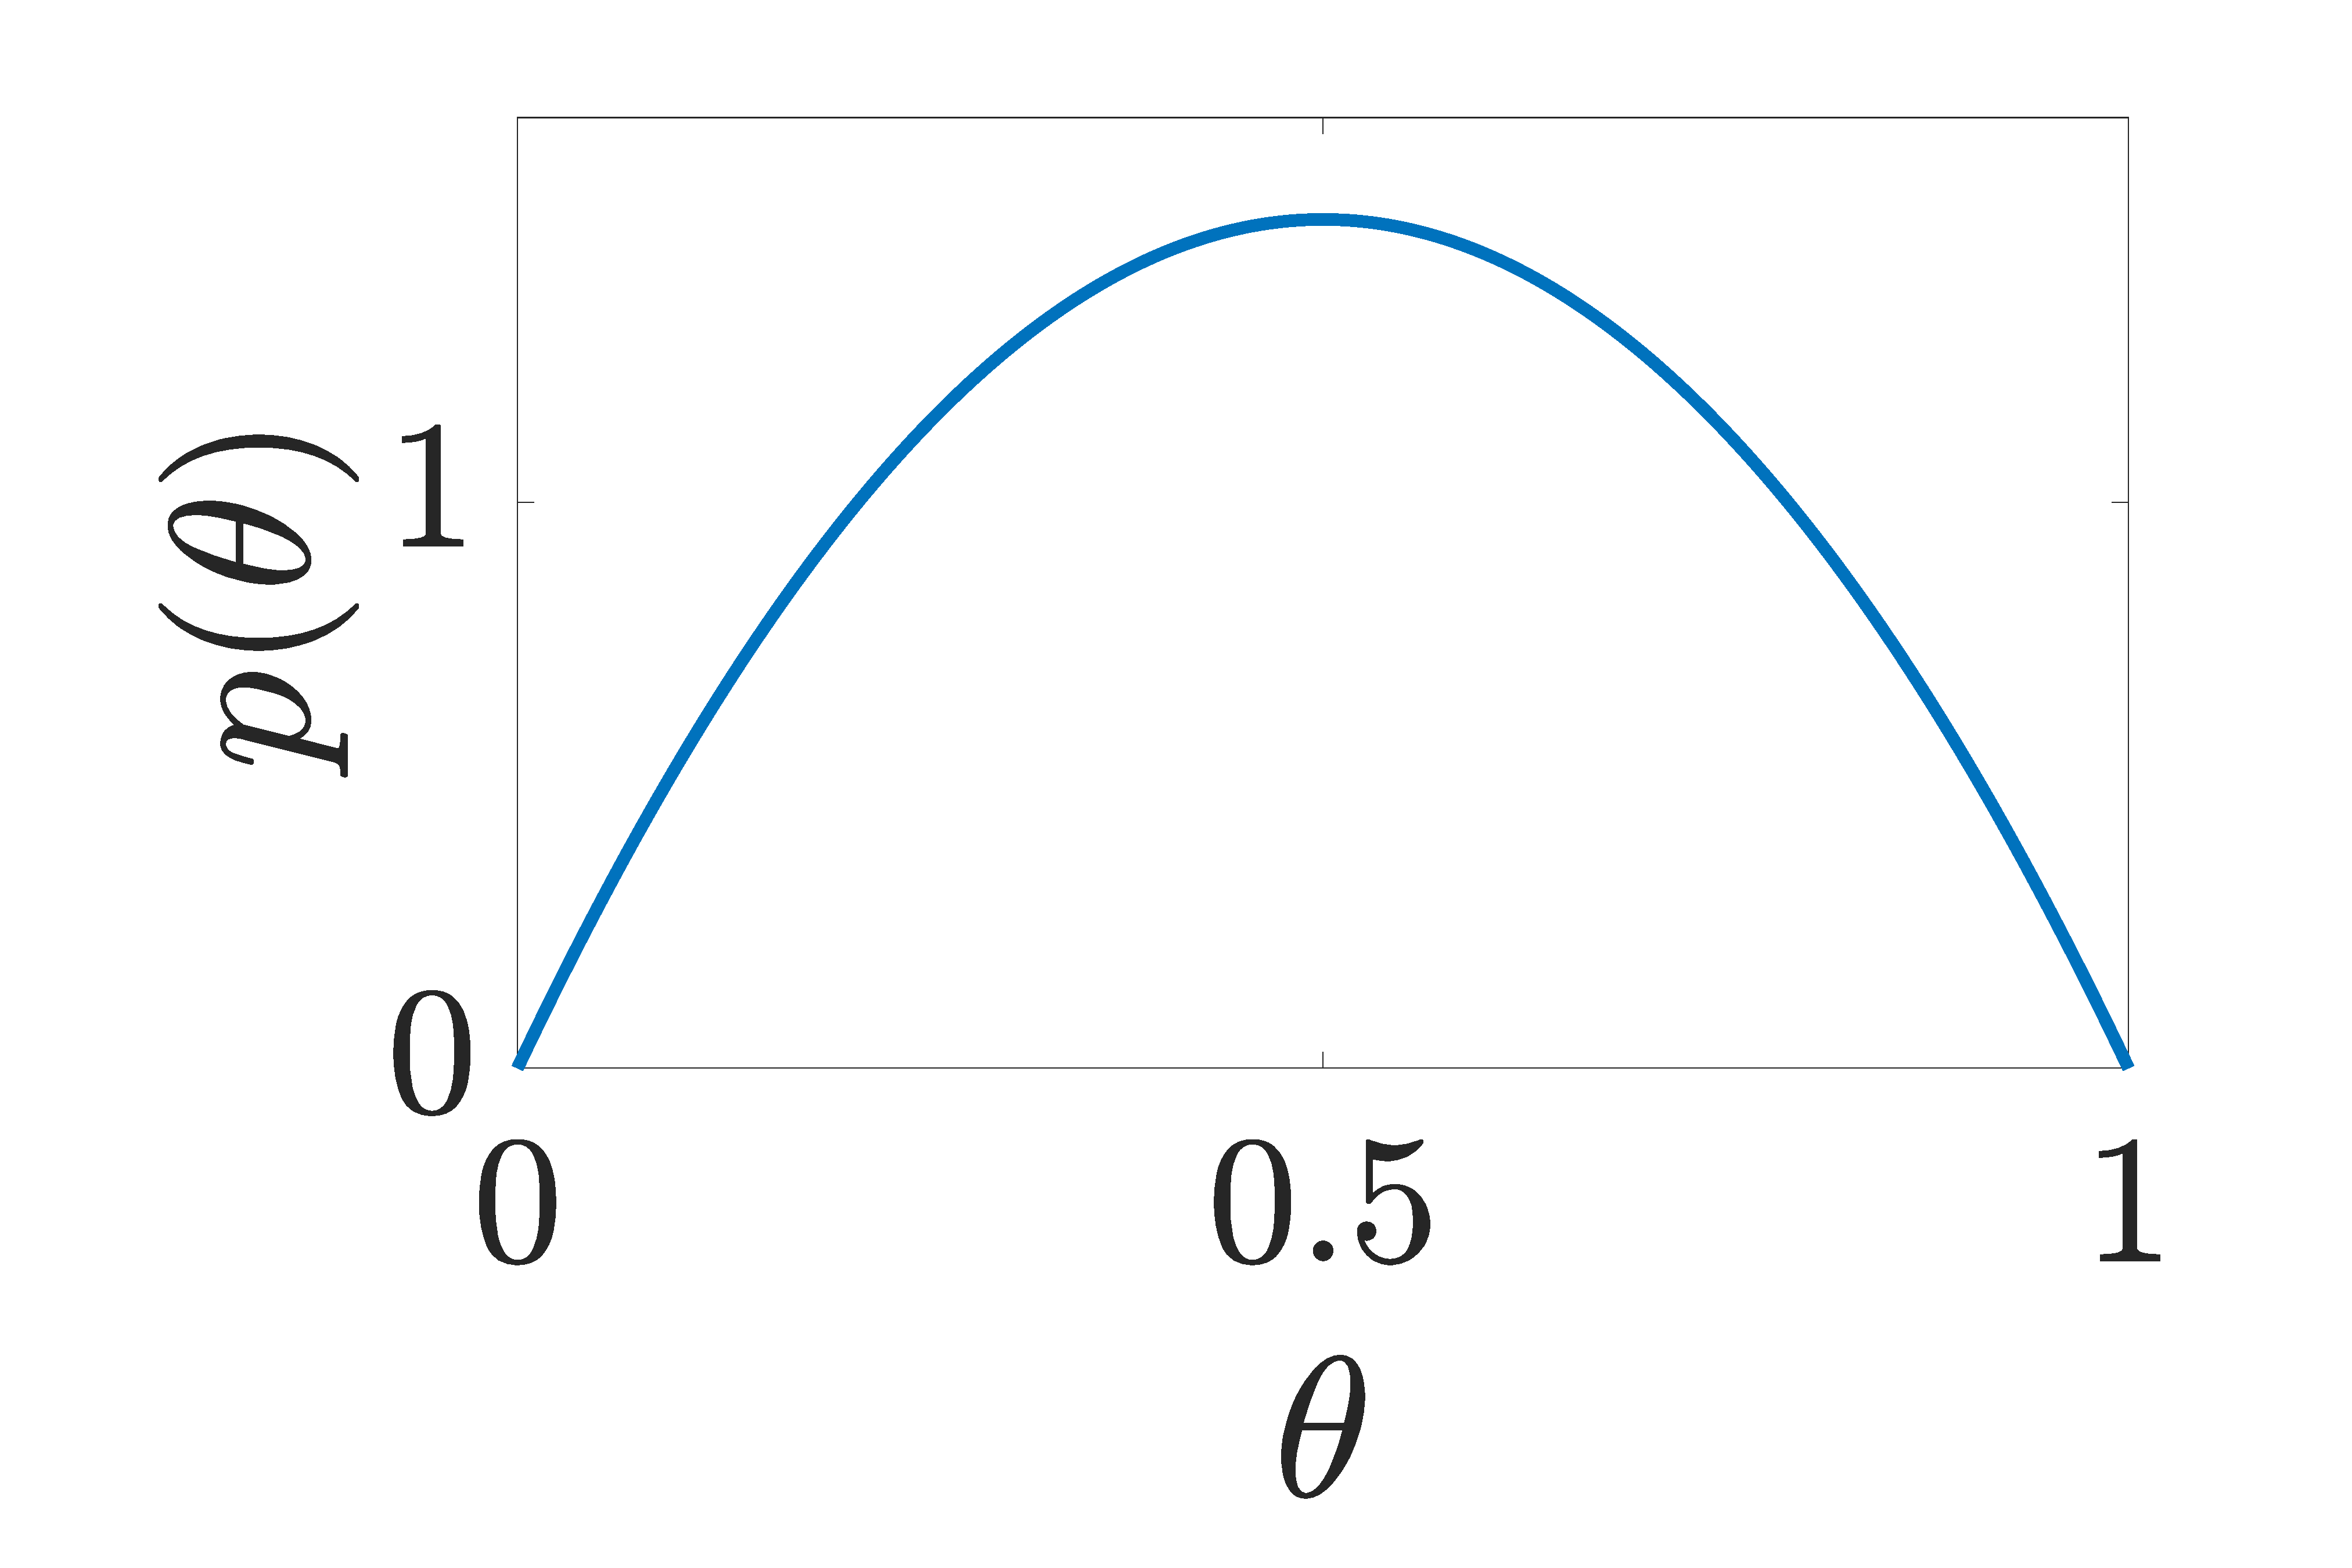
\includegraphics[width=\textwidth]{coin_flip_0}
		\caption{Prior \label{fig:inf:coin_flip:0}}
	\end{subfigure}
	\begin{subfigure}[t]{0.24\textwidth}
			\hspace{-10pt}
		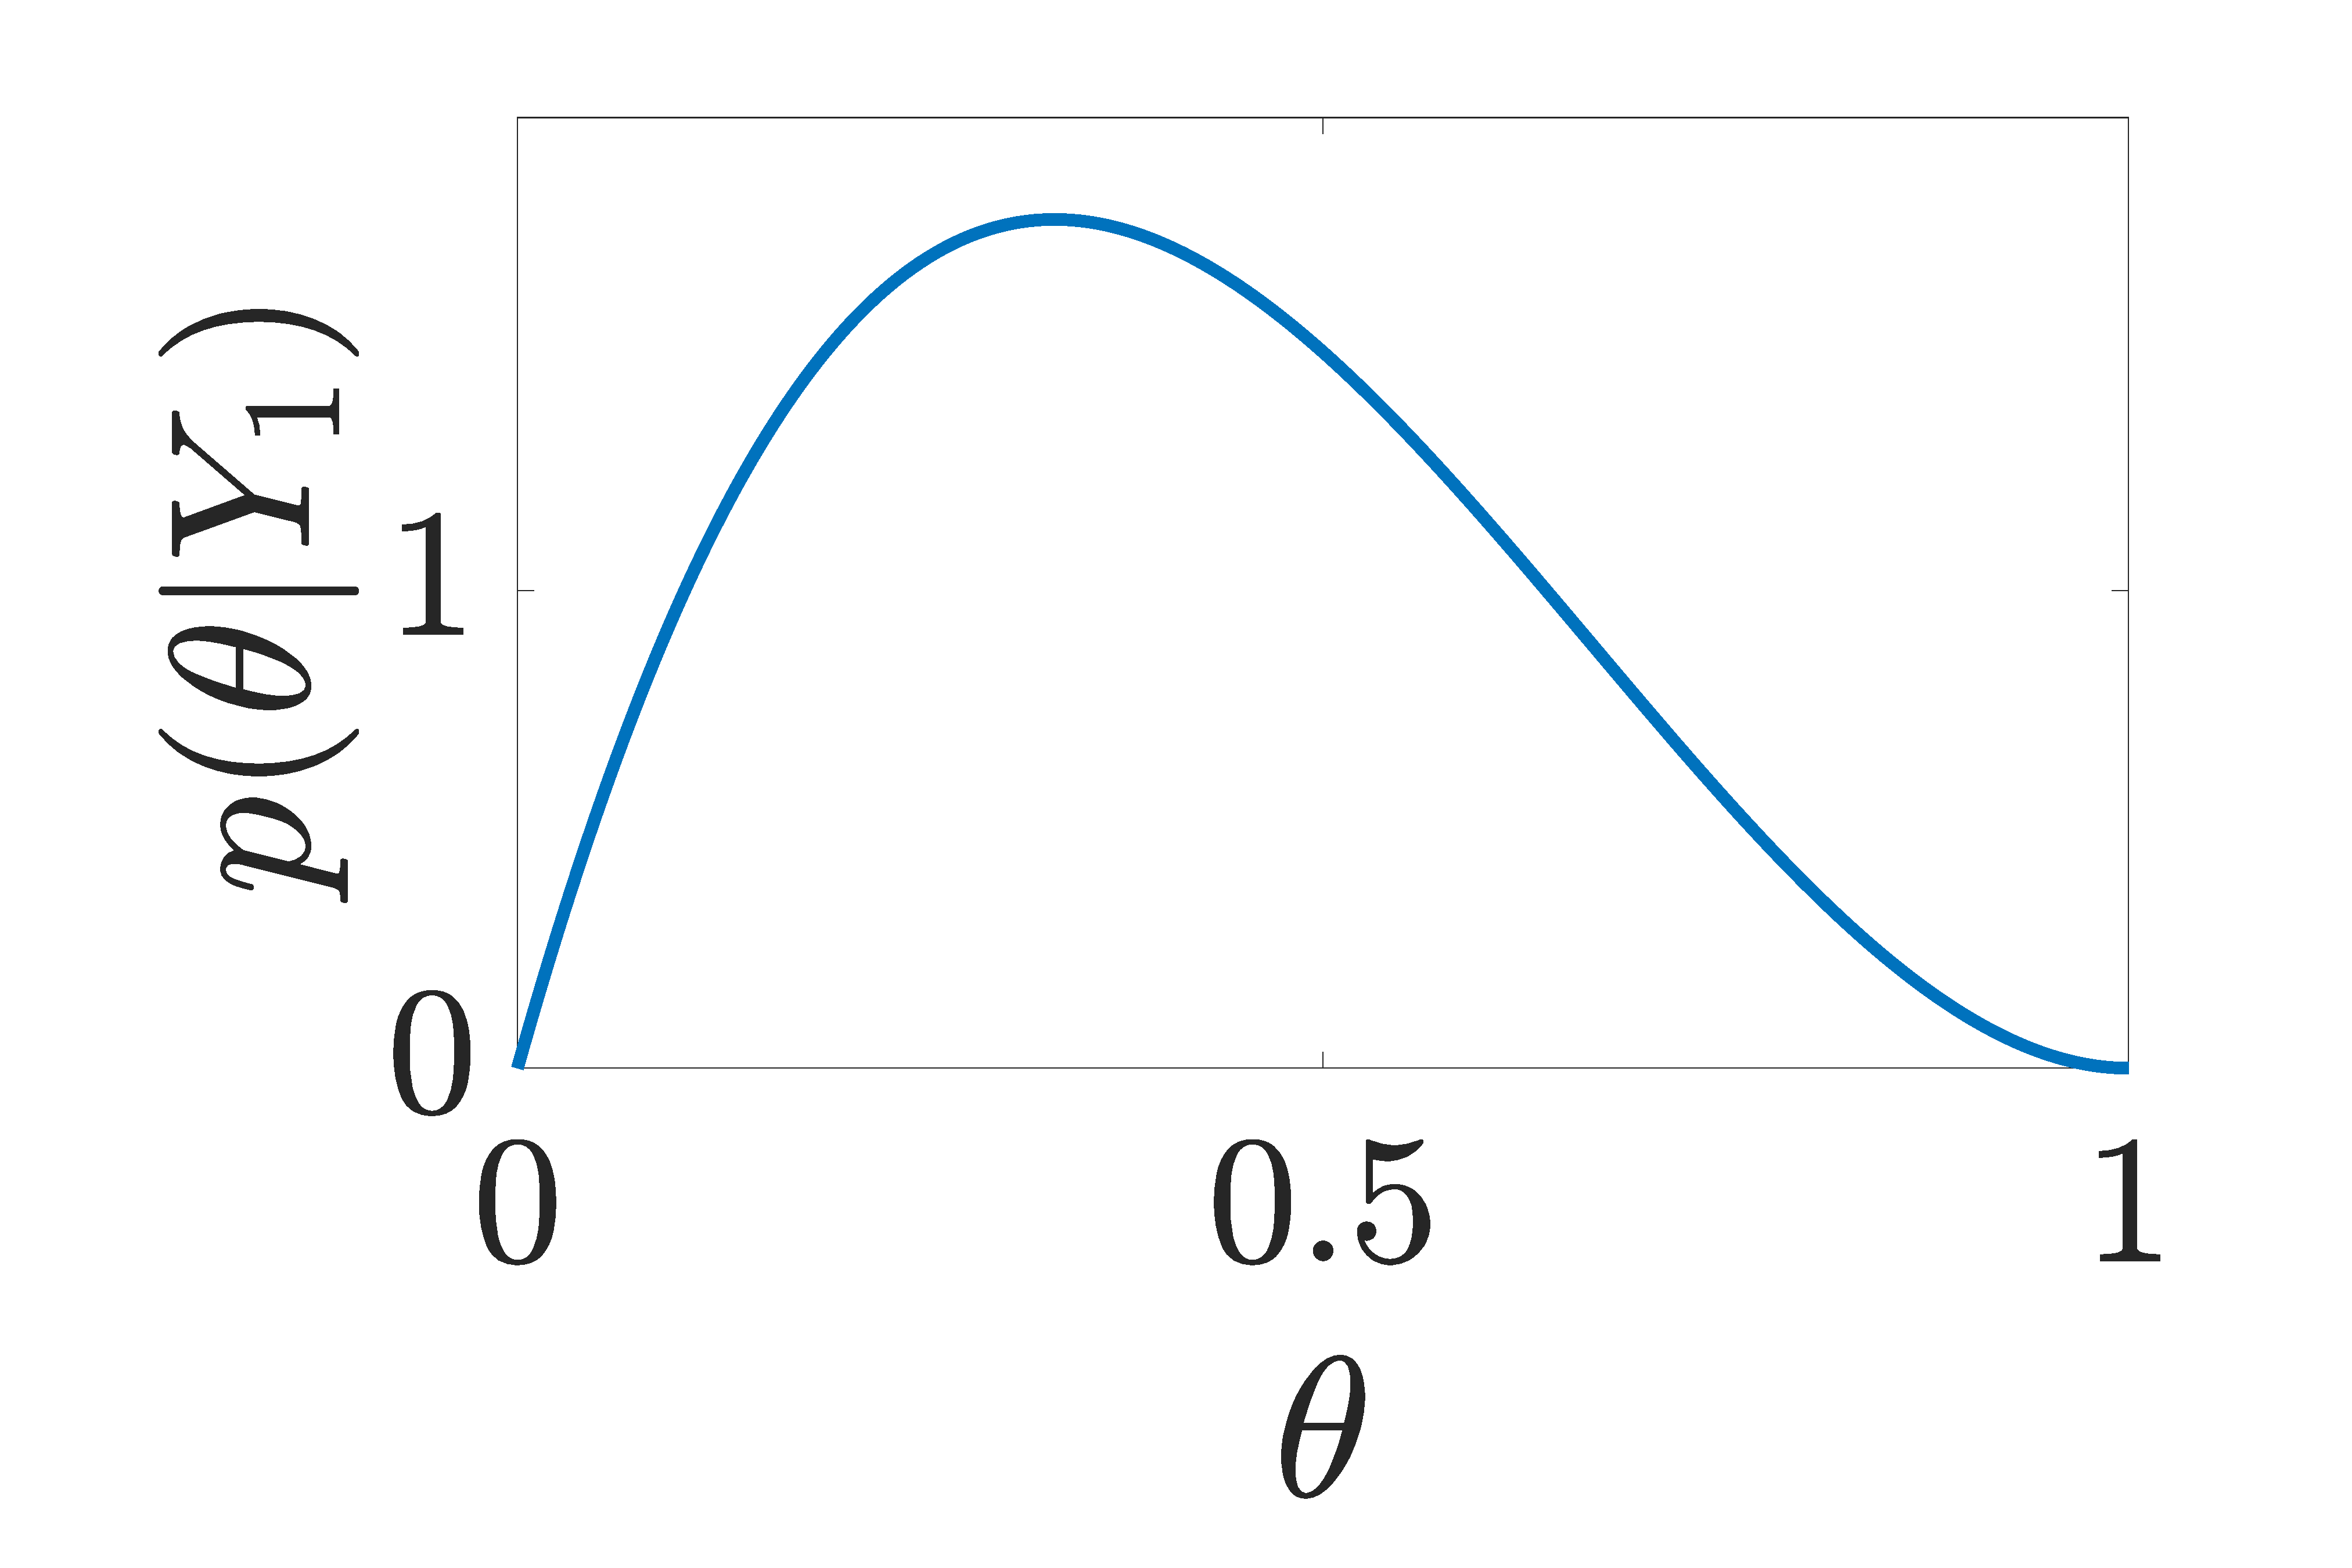
\includegraphics[width=\textwidth]{coin_flip_1}
		\caption{Posterior 1 flip \label{fig:inf:coin_flip:1}}
	\end{subfigure}
		\hspace{-3pt}
	\begin{subfigure}[t]{0.24\textwidth}
		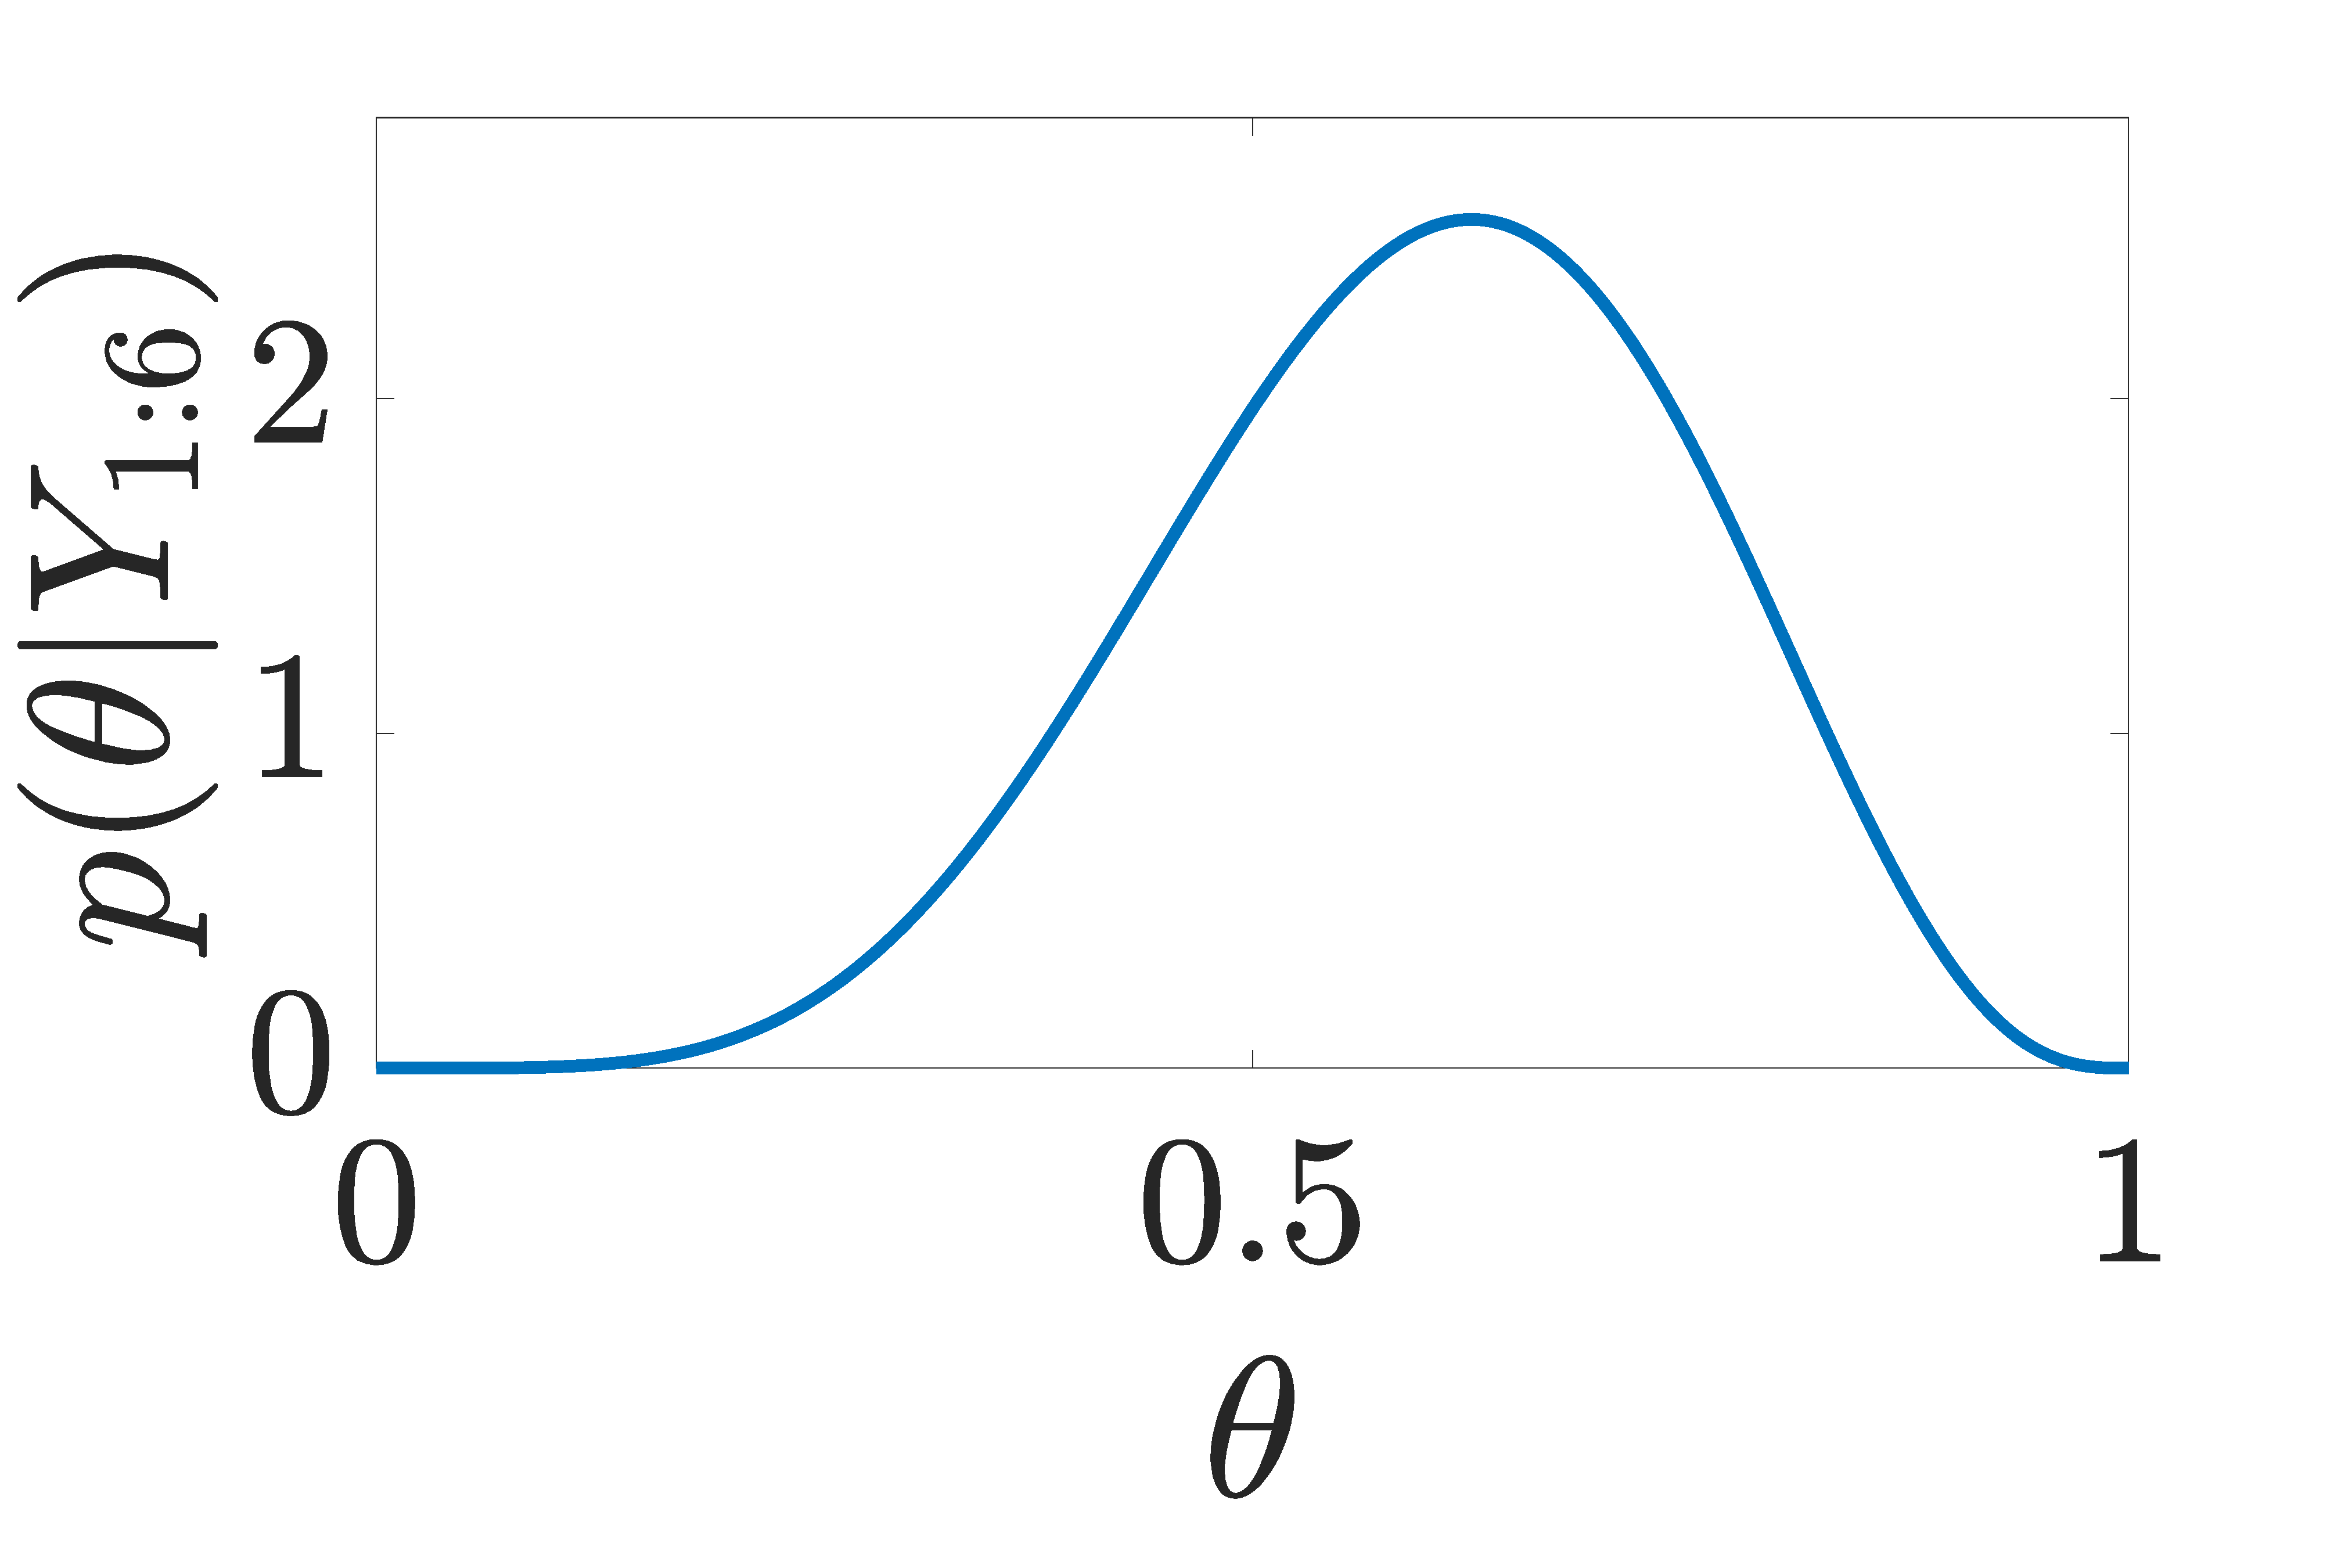
\includegraphics[width=\textwidth]{coin_flip_6}
		\caption{Posterior 6 flips \label{fig:inf:coin_flip:6}}
	\end{subfigure}
	\hspace{3pt}
	\begin{subfigure}[t]{0.24\textwidth}
		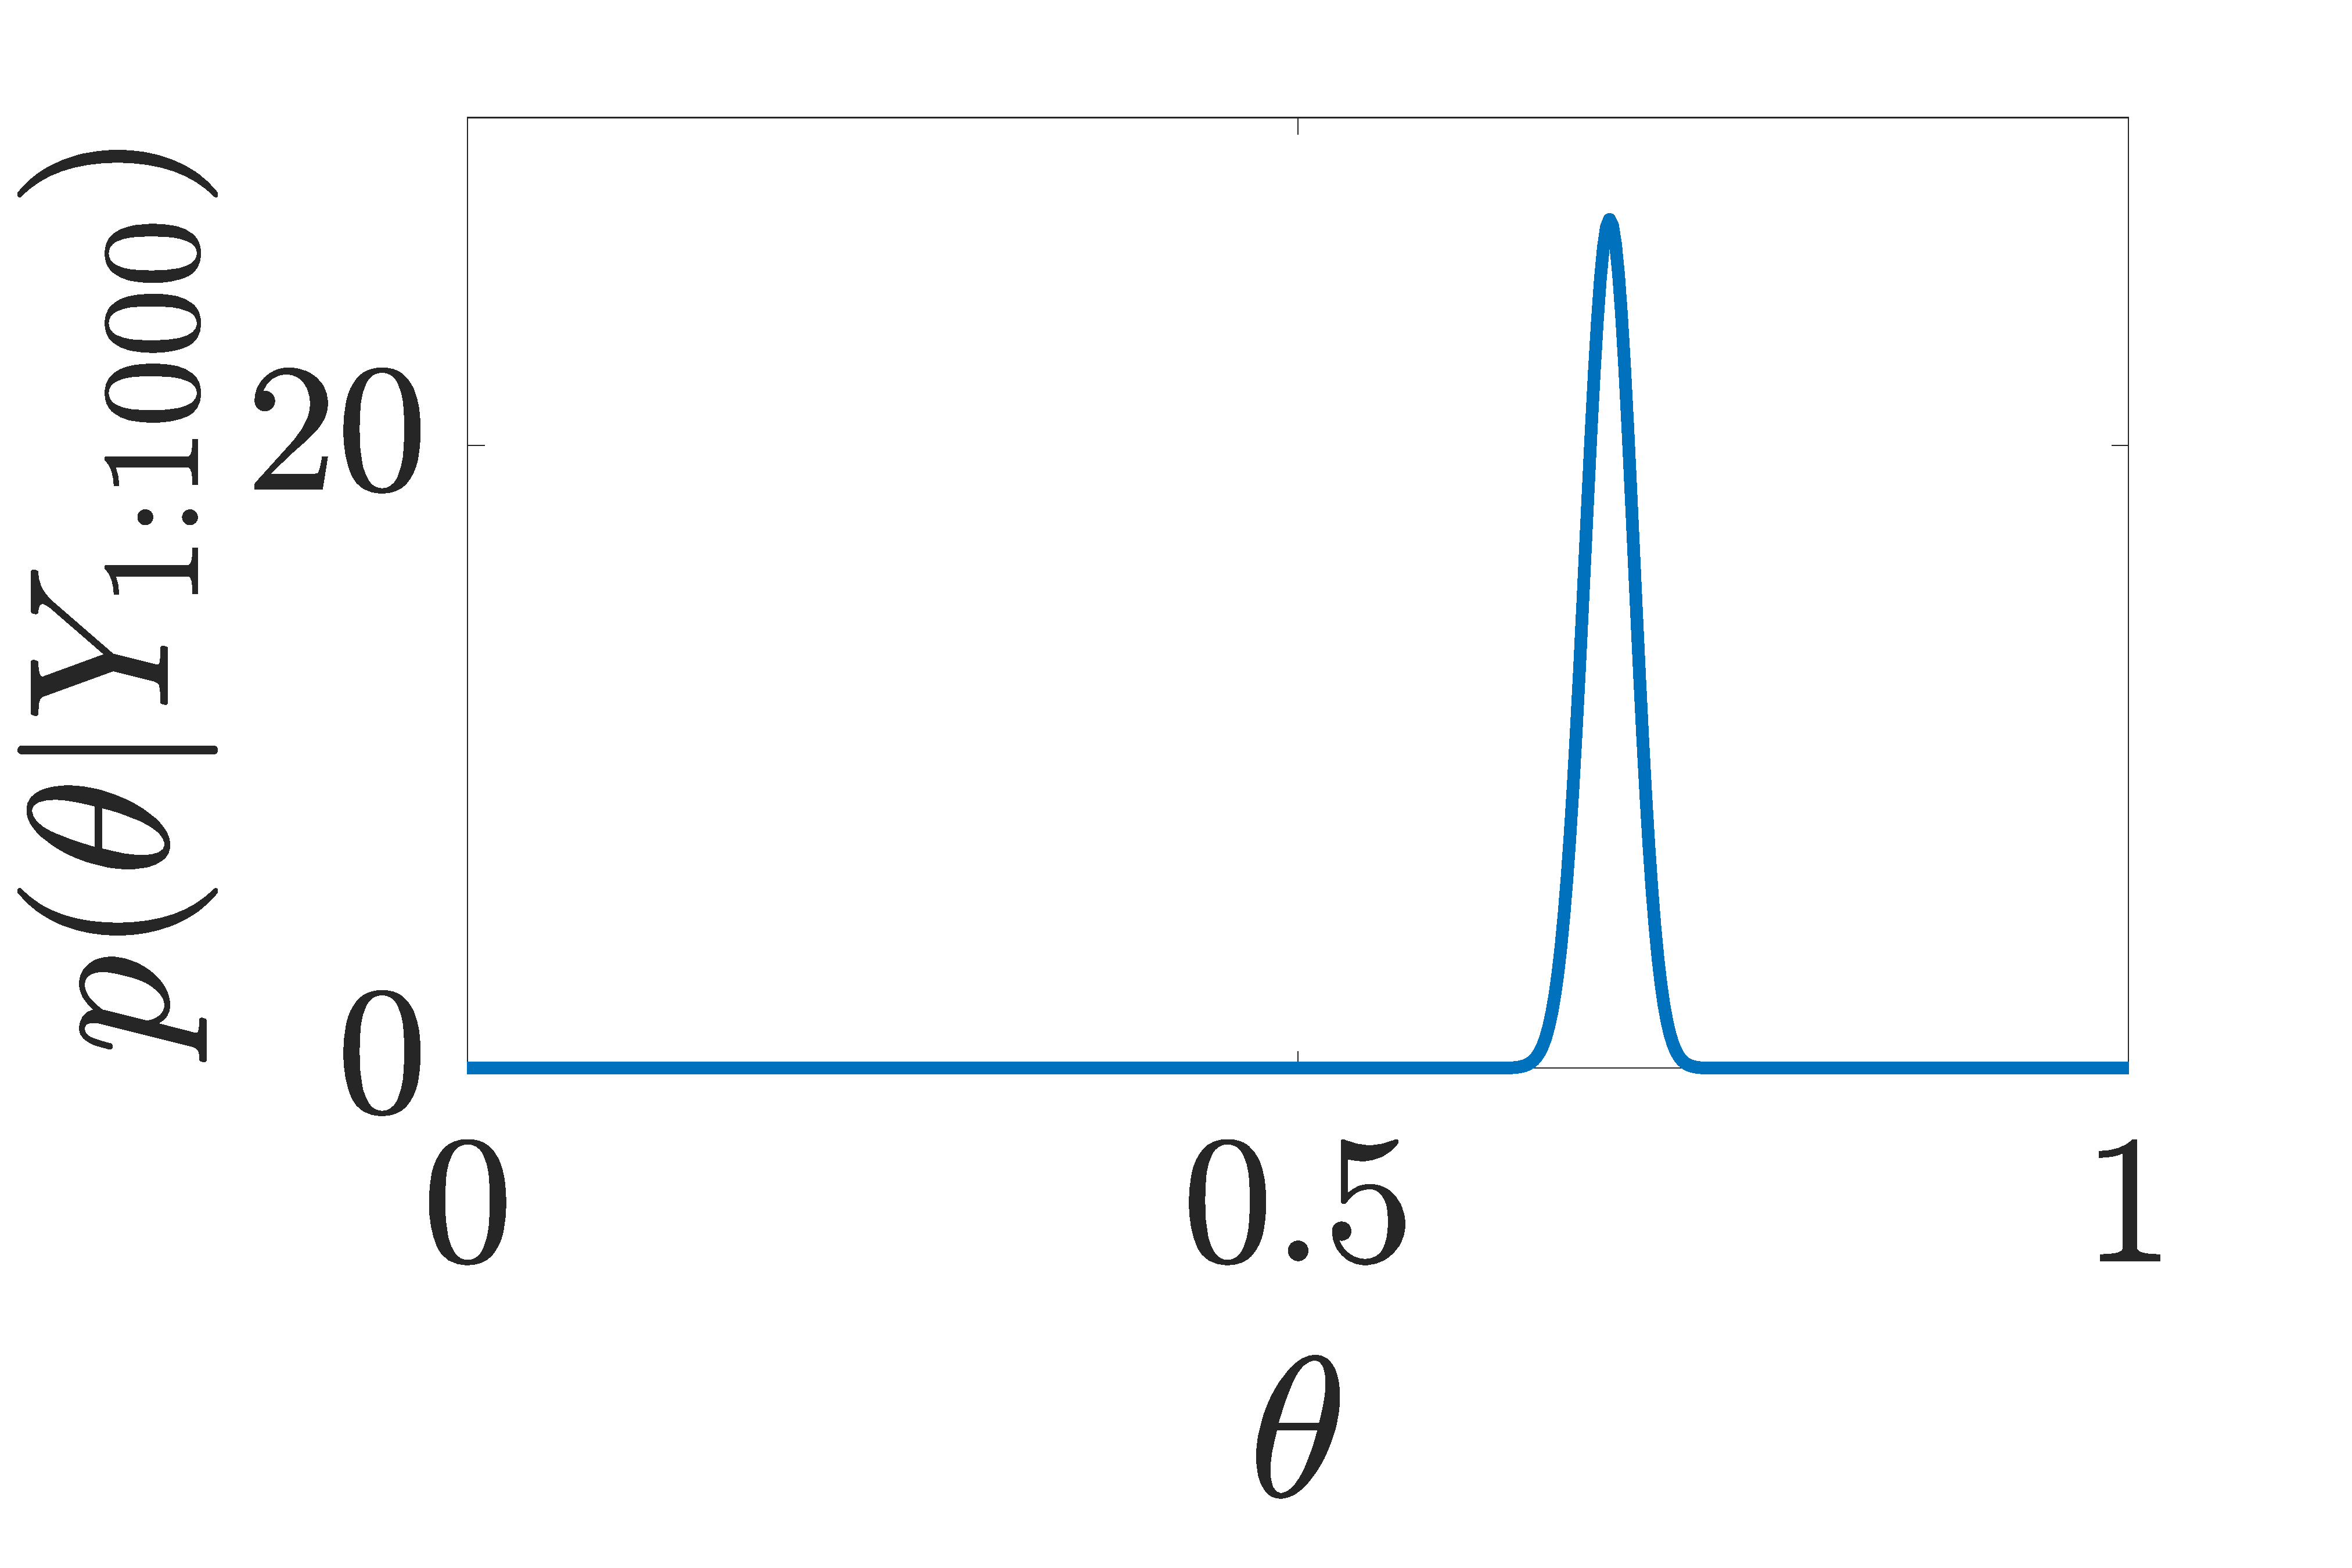
\includegraphics[width=\textwidth]{coin_flip_1000}
		\caption{Posterior 1000 flips \label{fig:inf:coin_flip:1000}}
	\end{subfigure}
	\caption{Prior and posteriors for coin flip example after different numbers
		of observations. \vspace{-5pt}
		\label{fig:inf:coin_flip}}
\end{figure}

If we now flip the coin again, our previous posterior~\eqref{eq:prob:beta_post_1} becomes our
prior and we can incorporate the new observations in the same way.  
Through our previous conjugacy result, then if we observe $n_{H}$ heads
and $n_{T}$ tails and our prior is $\textsc{Beta}(\theta ; \alpha, \beta)$ then our posterior is
$\textsc{Beta}(\theta ; \alpha+n_H, \beta+n_T)$.
Thus if our sequence of new
observations is $HTHHH$ then our new posterior is
\begin{align}
p(\theta | y_1,\dots,y_6) = \frac{p(y_2,\dots,y_6 | \theta)p(\theta | y_1)}
{\int p(y_2,\dots,y_6 | \theta)p(\theta | y_1) d\theta} = \textsc{Beta}\left(\theta ; 6,4\right),
\end{align}
which is shown in Figure~\ref{fig:inf:coin_flip:6}.  We see now that our belief for the probability of heads
has shifted higher and that the uncertainty has reduced because of the increased number
of observations.
After seeing a total of $1000$ observations as shown in Figure~\ref{fig:inf:coin_flip:1000}, we
find that the posterior has predominantly collapsed down to a small range of $\theta$.

Having calculated our posterior, we can now make
predictions using the \emph{posterior predictive distribution} which marginalizes out over
the parameters.  For the coin flip case, we have
\begin{align}
\label{eq:bayes:post-pred}
p( y_{N+1}=H | y_{1:N}) &= \int p(y_{N+1}=H, \theta | y_{1:N}) d\theta
= \int p(y_{N+1}=H | \theta) p(\theta | y_{1:N})  d\theta \nonumber \\
&= \int  \theta \; \textsc{Beta}(\theta ; \alpha+n_H, \beta+n_T) d\theta 
%= \int  
%\frac{\Gamma(\alpha+\beta)}{\Gamma (\alpha) \Gamma(\beta)} 
%\theta^{\alpha} (1-\theta)^{\beta-1} d\theta = 
%\frac{\Gamma(\alpha+\beta) \Gamma (\alpha+1)}{\Gamma (\alpha) \Gamma(\alpha+1+\beta)} \nonumber \\
=\frac{\alpha+n_H}{\alpha+n_H+\beta+n_T}
\end{align}
where we have used the known result for the mean of the Beta distribution.
The role of the parameters $\alpha$ and $\beta$ in our prior now become apparent
-- they take on the role of pseudo-observations.  Our prediction is in line with the
empirical average from seeing $\alpha+n_H$ heads and $\beta+n_T$ tails.  The larger
$\alpha+\beta$ is then the strong our prior compared to the observations, while we
can skew towards heads or tails being more likely by changing the relative values of $\alpha$
and $\beta$.

More generally the posterior predictive distribution will depend on a queried input point.
To demonstrate this, consider the example of a Bayesian linear regression from inputs $x\in\real^D$
to outputs $y\in\real$.  Assume that we have $N$ observations $\mathcal{D} = \{x_n,y_n\}_{n=1}^N$
and let $\mathbf{x}=[x_1,\dots,x_N]^T$ and $\mathbf{y}=[y_1,\dots,y_N]^T$ respectively be 
a $N\times D$ matrix and a column vector whose rows correspond to the different data points.
Our regression is of the form $y_n= x_n^T\mathbf{w}+b+\epsilon_n$ where $\mathbf{w}\in\real^D$, $b\in\real$
and each $\epsilon_n \iid \mathcal{N}(0,\sigma^2)$.  This implies a likelihood of
\begin{align}
\label{eq:bayes:linear-reg-lik}
p(\mathbf{y}|\mathbf{x},\mathbf{w},b,\sigma) = \prod_{n=1}^{N} p(y_n | x_n, \mathbf{w}, b, \sigma) = 
\prod_{n=1}^{N} \mathcal{N}(y_n;x_n^T\mathbf{w}+b,\sigma^2).
\end{align}
For simplicity, we will assume that $\sigma$ and $b$ are known fixed parameters,
but we will put a prior on $\mathbf{w}$, namely $p(\mathbf{w}) = \mathcal{N}(\mathbf{w};\mathbf{0},C)$
where $C$ is a fixed covariance matrix, in order to perform inference.
%% and $s$ a fixed scalar standard deviation.
%We further assume that $p(\mathbf{w},b | \sigma) = p(\mathbf{w}) p(b) $, i.e. that all
%three parameters are independent under the prior.
To make predictions, we first calculate the posterior
\begin{align}
p(\mathbf{w}| \mathcal{D}, b,\sigma) &= \mathcal{N}(\mathbf{w};\mathbf{0},C)
\prod_{n=1}^{N} \mathcal{N}(y_n;x_n^T \mathbf{w}+b,\sigma^2) = \mathcal{N}\left(\mathbf{w} ; m, S\right) \\
\mathrm{where} \quad m &= S^{-1} \mathbf{x}^T \left(\mathbf{y}-b\right)/\sigma^2 \quad
\mathrm{and} \quad S = \left( C^{-1}+\frac{\mathbf{x}^T\mathbf{x}}{\sigma^2}\right)^{-1}. \nonumber
%&= \mathcal{N}\left(\mathbf{w} ; \left( C^{-1}+\frac{\mathbf{x}^T\mathbf{x}}{\sigma^2}\right)^{-1} 
%\frac{\mathbf{x}^T \left(\mathbf{y}-b\right)}{\sigma^2},
%\left( C^{-1}+\frac{\mathbf{x}^T\mathbf{x}}{\sigma^2}\right)^{-1} \right),
\end{align}
We have omitted the necessary linear algebra (see for example~\cite{bishop2006pattern}
Sections 2.3.3 and 3.3)
but note the conjugacy between
the normal distribution and itself.  Prediction now uses the posterior predictive, marginalizing
over the parameters in the same manner as the coin flip example.  Here though, we are interested
in predicting the output $\tilde{y}$ at a particular input point $\tilde{x}$ for which we have
\begin{align}
p(\tilde{y}| \tilde{x},\mathcal{D}, b,\sigma) &= \int p(\tilde{y}| \tilde{x},\mathbf{w}) 
p(\mathbf{w}| \mathcal{D}, b,\sigma) d\mathbf{w} 
= \int \mathcal{N}(\tilde{y};\tilde{x}^T\mathbf{w}+b,\sigma^2)
\mathcal{N}\left(\mathbf{w} ; m, S\right) d\mathbf{w} \nonumber \\
&= \mathcal{N} \left(\tilde{y} \; ; \;\tilde{x}^Tm+b, \; \tilde{x}^T S^{-1}\tilde{x}+\frac{1}{\sigma^2} \right)
\end{align}
which again follows from standard results for Gaussian distributions.  We, therefore, have
an analytic predictive distribution at any possible input point.
Though this linear regression example might seem overly simple for practical purposes, we
will see in Section~\ref{sec:opt:GPs} that substantially more advanced models, such as
Gaussian processes, can be viewed as linear regressions between a set of features on the inputs $\phi(x)$
and the output $y$.

The models we have introduced so far are specific examples of Bayesian modeling and will
clearly only be applicable or appropriate in very particular scenarios.  
%However, the only restrictions we
%have in order to carry out Bayesian modeling is that the prior and likelihood are valid probability distributions
%(in practice even these requirements can often be relaxed).  
Bayesian modeling is at its heart a
generative approach and its real power will be when we design a rich and expressive \emph{generative model} 
that reflects our application-specific knowledge.  In other words, we can define our model
by carefully constructing a stochastic process that describes how the parameters  and data are generated.  For
our object recognition example at the start of the section, this would correspond to a graphics generator for
sampling scenes.
More generally, the model corresponds to the joint distribution on parameters and data $p(\theta,\mathcal{D})$.
We can then think of observing real data as refining our model through \emph{conditioning}, providing an updated distribution
on the parameters $p(\theta|\mathcal{D})$ and subsequent predictions that incorporate the information from the data.  The more
flexible we make our generative model, the more we can make it represent the data.  The less flexible
we make the generative model, the more weighting is given to our prior assumptions.

We finish by making a technical point of note about the behavior of Bayesian methods in the limit of large
data.  Assume that our likelihood model $p(\mathcal{D}|\theta)$ is correct such that the data $\mathcal{D} = y_{1:N}$
is generated according to 
$p(y_{1:N} | \theta^*)$ where $\theta^*$ are the (finite) set of ground truth parameters 
and the prior $p(\theta)$ satisfies $p(\theta^*)>0$.  Informally speaking, the Bernstein-Von Mises theorem now states
that in the limit of large $N$, the posterior distribution $p(\theta | y_{1:N})$ converges to a normal distribution 
with mean $\theta^*$ and variance of order $O(1/N)$ 
(i.e. it decreases at a rate $1/N$)~\citep{doob1949application,freedman1963asymptotic}.  This is a hugely important
result in Bayesian statistics as it demonstrates that, when our model assumptions are correct, we converge to the true parameters 
and the posterior becomes independent of the prior when we are provided with sufficient data.  It further transpires that when no such $\theta^*$ exists (i.e. our model is misspecified), the convergence
is instead to the parameters $\hat{\theta}$ which minimize the Kullback-Leibler (KL) divergence\footnote{The KL divergence
	can informally be thought of as a measure of discrepancy between two distributions.  Though
	it is not symmetric in its inputs, it is always non-negative and zero if and only if the two distributions are the same.} to the true data generating
distribution $p^*(y_{1:N})$, namely
\begin{align}
\hat{\theta} = \argmin_{\theta} \textsc{KL}\left(p^*(y_{1:N}) \| p(y_{1:N} | \theta)\right)
= \argmin_{\theta} \int p^*(y_{1:N}) \log \left(\frac{p^*(y_{1:N})}{p(y_{1:N}|\theta)}\right) dy_{1:N}.
\end{align}
See for example~\citep{kleijn2012bernstein} and the references therein for further details.
% !TEX root = ../main.tex

\section{Graphical Models}
\label{sec:bayes:paradigm:graph}

Generative models will typically have many variables and a complex \emph{dependency structure}.
In other words, many of variables will be conditionally independent of one another given values for
other variables.  Graphical models are a ubiquitously used method for representing and reasoning
about generative models with a particular focus on the dependency structure.  At a high-level, they
capture how the joint probability distribution can be broken down into a product of different factors, 
each defined over
a subset of the variables.  They are formed of a number of connected nodes, where each node
represents a random variable in the model and each variable has its own node.  Links between nodes in
the model represent dependencies: any two connected nodes have an explicit dependency.
Various independence assumptions can be deduced from the graphical model, though the exact nature
of these deductions will depend on the type of graphical model -- nodes without direct links
between them will often still be dependent.

Graphical models can be separated into two distinct classes: directed graphical
models and undirected graphical models.  Undirected graphical models, also known as Markov random
fields, imply no ordering on their factorization and are used only to express conditional independences
between variables.  They are used in scenarios where it is difficult to specify the target distribution in a
structured generative way, e.g. in Boltzmann machines~\citep{ackley1985learning}.  To give 
a more concrete example, if modeling whether it will rain at various locations then there
is a clear dependence between nearby locations, but not a natural ordering to the joint probability
distribution of where it will rain.   Independence in undirected graphical models can be deduced
through the \emph{global Markov property} which states that any two non-intersecting subsets of the 
variables $A$ and $B$ are
conditionally independent given a third, separating, subset $C$ if there is no path between $A$ and
$B$ that does not pass through $C$.  This means, for example, that each variable is conditionally
independent of all the other variables given its neighbors.

Our main focus, though, will instead be on directed graphical models and in particular directed acyclic 
graphical models (DAGs), i.e. directed graphical models containing no cycles or loops one can follow 
and arrive back in the starting position.  DAGs, also known as Bayesian networks, are particularly
useful in the context of Bayesian modeling because they can be used to express \emph{casual relationships}.
As such, they can be used as a piecewise explanation for how the joint distribution is generated.
Not only does this form a natural means to describe and design models in the first place, 
we can carefully order the breakdown to factorize the distribution into only terms we know.  For example,
in the linear regression model, we did not know (at least when the model was first defined) 
$p(\mathcal{D})$ but we did know $p(\mathbf{w})$ and $p(\mathcal{D} | \mathbf{w})$.  Therefore even
though we could factorize our joint $p(\mathcal{D}, \mathbf{w})$ as 
$p(\mathbf{w} | \mathcal{D})p(\mathcal{D})$ and construct a DAG this way, it is much more convenient
to factorize and construct the DAG the other way round, namely as 
$p(\mathcal{D} | \mathbf{w})p(\mathbf{w})$.
We will generally not have access to all possible factorizations
in an analytic form as otherwise there would be no need to perform inference.
As a rule-of-thumb, when we define a model using a DAG, we need to be able to define the 
probability of each variable given its \emph{parents}, i.e. all the nodes with links from that node
towards the node the question.

The demonstrate this factorization more explicitly and give a concrete example of a DAG, consider a joint model
$p(a,b,c)$.  By the product rule, we can break down this joint distribution into a number of different
factorizations, but some will typically be more useful than others.  Imagine a medical diagnostic
example where $a$ represents lifestyle and genetic factors of a patient such as whether they smoke
or have unknown preexisting conditions, 
$b$ represents the presence of lung cancer, and $c$ represents symptoms 
such as a persistent cough.  Here we have the following natural breakdown of the joint distribution
\begin{align}
\label{eq:bayes:example-graph}
p(a,b,c) = p(a) p(b|a) p(c|a,b).
\end{align}
\begin{wrapfigure}{r}{0.35\textwidth}
	\vspace{-12pt}
	\centering 
	\resizebox{.32\textwidth}{!}{
		% !TEX root = ../../main.tex

\begin{tikzpicture}

\node[obs]                               (c) {$c$};
\node[latent, above=of c, xshift=-1.2cm] (a) {$a$};
\node[latent, above=of c, xshift=1.2cm]  (b) {$b$};

\edge {a,b} {c} ; %
\edge {a} {b} ; %

\end{tikzpicture}
	}
	\caption{Simple example DAG corresponding to~\eqref{eq:bayes:example-graph}
		\label{fig:bayes:simple-graph}}
	\vspace{-10pt}
\end{wrapfigure}
The lifestyle and genetic factors will generally either be known or can be estimated from tests or
simply prevalence within the population.  Given these factors, the likelihood of somebody developing
lung cancer can be modeled using existing data and domain expertise.   Given the lifestyle and
genetic factors and the knowledge of whether lung cancer is present, we can predict what
symptoms might be observed.  We can express our model and this factorization using
the DAG shown in Figure~\ref{fig:bayes:simple-graph}.
  Here we have shaded in $c$ to express the fact that this is
observed.  The graphical model expresses our dependency structure as we have the probability
of each node given its parents.  As shown in~\eqref{eq:bayes:example-graph}, the product of
all these factors is equal to our joint distribution.  The DAG has thus formed a convenient means
of representing our generative process.

Clearly, our aim for this problem will be to find the probability cancer is present given
the symptom, i.e. $p(b|c)$, which will
require Bayesian inference.
An important feature of the breakdown of graphical models will become apparent when we
consider how we can conduct such inference for more a general class of 
models where the solution is not analytic in Chapter~\ref{chp:inf}.  Here knowing the dependency
structure and, in particular, the independence relationships, will be essential to many inference 
schemes such as message passing schemes.

A natural question is now how can we deduce the independence relationships from a DAG?
This can be done by introducing the notion of \emph{d-separation}~\citep{pearl2014probabilistic}.
Consider three arbitrary, non-intersecting, subsets $A$, $B$, and $C$ of our DAG.  $A$ and $B$
are conditionally independent given $C$ if there are no \emph{unblocked} paths from $A$ to $B$
(or equivalently from $B$ to $A$), in which case $A$ is said to be d-separated from $B$ by $C$.  
Paths do not need to be in the directions defined by the DAG but are blocked if either
\begin{enumerate}
		\setlength\itemsep{-0.1em}
	\item Consecutive arrows both point towards a node that is not in and
	has no descendants in $C$, i.e. we cannot get to any of the nodes in $C$ by following the arrows
	from this node.
	\item Consecutive arrows meet at a node in $C$ and one of them
	points away from the node.
\end{enumerate}
Note that only the first of these rules is necessary for establishing marginal independence
between nodes as this rule can still be used when $C$ is empty.
Examples of blocked paths are shown in Figure~\ref{fig:bayes:blocked-graphs} while examples of unblocked paths
are shown in Figure~\ref{fig:bayes:unblocked-graphs}, explanations for which are given in the captions.
For a more comprehensive introduction to establishing independence in DAGs, we
refer the reader to Section 8.2 of~\cite{bishop2006pattern}.

\begin{figure}[t]
	\centering 
	\begin{subfigure}[t]{0.32\textwidth}
		\centering
		\resizebox{0.9\textwidth}{!}{
		% !TEX root = ../../main.tex

\begin{tikzpicture}

\node[obs]                               (c) {$c$};
\node[latent, above=of c, xshift=-1.2cm] (a) {$a$};
\node[latent, above=of c, xshift=1.2cm]  (b) {$b$};

\edge {a} {c} ; %
\edge {c} {b} ; %

\end{tikzpicture}}
		\caption{\label{fig:bayes:block1}}
	\end{subfigure}
	\begin{subfigure}[t]{0.32\textwidth}
		\centering
		\resizebox{0.9\textwidth}{!}{
		% !TEX root = ../../main.tex

\begin{tikzpicture}

\node[obs]                               (c) {$c$};
\node[latent, below=of c, xshift=-1.2cm] (a) {$a$};
\node[latent, below=of c, xshift=1.2cm]  (b) {$b$};

\edge {c} {a} ; %
\edge {c} {b} ; %

\end{tikzpicture}}
		\caption{\label{fig:bayes:block2}}
	\end{subfigure}
	\begin{subfigure}[t]{0.32\textwidth}
		\centering
		\resizebox{0.9\textwidth}{!}{
		% !TEX root = ../../main.tex

\begin{tikzpicture}

%\node[latent]  (a) {$a$};
%\node[latent, right=2.4cm of a]  (b) {$b$};
%\node[latent, below= of a, xshift=1.2cm] (d) {$d$};
%%\node[latent, right=1.8cm of d]             (e) {$e$};
%
%%\edge {d} {e} ; %
%\edge {a} {d} ; %
%\edge {b} {d} ; %

\node[latent]                               (d) {$d$};
\node[latent, above=of d, xshift=-1.2cm] (a) {$a$};
\node[latent, above=of d, xshift=1.2cm]  (b) {$b$};

\edge {a} {d} ; %
\edge {b} {d} ; %

\end{tikzpicture}}
		\caption{\label{fig:bayes:block3}}
	\end{subfigure}
	\caption{Examples of DAGs blocked between $a$ and $b$.  \textbf{(a)} is blocked
		by the second rule of d-separation.  More specifically we have 
		$p(b|a,c)=\frac{p(a,b,c)}{p(a,c)} = \frac{p(a)p(c|a)p(b|c)}{p(a)p(c|a)} = p(b|c)$.
		\textbf{(b)} is blocked by the first rule of d-separation.  Here we have
		$p(b|a,c)=\frac{p(c)p(a|c)p(b|c)}{p(c)p(a|c)} = p(b|c)$.  Consequently, for \textbf{(a)} 
		and \textbf{(b)} then $a$ and $b$ are conditionally independent given $c$ .
		\textbf{(c)} is an instead example of where $a$ and $b$ are \emph{marginally} independent.  Here
		the path between $a$ and $b$ is blocked because the the arrows meet head-to-head at 
		$d$ and neither $d$ nor any of its
		descendants are observed.  We thus have $p(b|a) = \frac{p(a)p(b)p(d|a,b)}{p(a)p(d|a,b)} = p(b)$.
		Note though that $a$ and $b$ are note conditionally independent given $d$ as
		the path becomes unblocked if this is observed (see Figure~\ref{fig:bayes:unblocked-graphs}).
		\label{fig:bayes:blocked-graphs}}
\end{figure}

\begin{figure}[t]
	\centering 
	\hspace{-15pt}
	\begin{subfigure}[t]{0.32\textwidth}
		\centering
		\resizebox{0.9\textwidth}{!}{
		% !TEX root = ../../main.tex

\begin{tikzpicture}

\node[latent]                               (d) {$d$};
\node[latent, above=of d, xshift=-1.2cm] (a) {$a$};
\node[latent, above=of d, xshift=1.2cm]  (b) {$b$};

\edge {a} {d} ; %
\edge {d} {b} ; %

\end{tikzpicture}}
		\caption{\label{fig:bayes:unblock1}}
	\end{subfigure}
	\begin{subfigure}[t]{0.32\textwidth}
		\centering
		\resizebox{0.9\textwidth}{!}{
		% !TEX root = ../../main.tex

\begin{tikzpicture}

\node[latent]                               (d) {$d$};
\node[latent, below=of d, xshift=-1.2cm] (a) {$a$};
\node[latent, below=of d, xshift=1.2cm]  (b) {$b$};

\edge {d} {a} ; %
\edge {d} {b} ; %

\end{tikzpicture}}
		\caption{\label{fig:bayes:unblock2}}
	\end{subfigure}
	\begin{subfigure}[t]{0.32\textwidth}
		\centering
		\resizebox{1.1\textwidth}{!}{
		% !TEX root = ../../main.tex

\begin{tikzpicture}

\node[latent]                               (d) {$d$};
\node[latent, above=of d, xshift=-1.2cm] (a) {$a$};
\node[latent, above=of d, xshift=1.2cm]  (b) {$b$};
\node[obs, right=1.2cm of d]             (c) {$c$};

\edge {d} {c} ; %
\edge {a} {d} ; %
\edge {b} {d} ; %

\end{tikzpicture}}
		\caption{\label{fig:bayes:unblock3}}
	\end{subfigure}
	\caption{Examples of DAGs unblocked between $a$ and $b$. For \textbf{(a)} then the path from $a$ to
		$b$ is not blocked by the d-separation rules.  Perhaps more intuitively, we have that
		$p(b|a) = \int p(b,d|a) dd = \int p(b|d)p(d|a) dd \neq p(b)$ unless $p(d|a)=p(d)$.
		Similarly there is an unblocked path for \textbf{(b)} from $a$ to $b$ as the path
		that does not pass through any observed nodes or nodes with both arrows points towards it.
		Here we have $p(b|a) = \frac{p(d)p(a|d)p(b|d)}{p(a)p(d|a,b)} \neq p(b)$ again in general.
		The path in \textbf{(c)} is unblocked because of the phenomenon of \emph{explaining away}.
		The first rule of d-separation does not apply here because $c$ is an observed descendant of
		$d$.  We thus have that $a$ and $b$ are marginally independent as per Figure~\ref{fig:bayes:block3},
		but not conditionally independent given $c$ (and/or $d$). The rationale for explaining away can be thought
		of in terms of events needing an explanation -- if two precursor events (here $a$ and $b$) can give rise 
		to a third event (here $c$), then
		the third event occurring but not the first precursor event implies that the second precursor
		event occurs.  Thus the two precursor events are correlated because one \emph{explains away} the other.
		As described in Section~\ref{sec:prob:cond}, one example of this is that if a speed camera is
		triggered and the camera is not malfunctioning, this implies the vehicle is speeding, even though
		the vehicle speeding and the camera malfunctioning are marginally independent.	
		\label{fig:bayes:unblocked-graphs}}
\end{figure}

In the simple example of Figure~\ref{fig:bayes:simple-graph} there were no independence relationships and so
we gain little from working with the DAG compared to just the joint probability distribution.
A more advanced example where there are substantial independence relationships which can
be exploited is shown in Figure~\ref{fig:bayes:hmm}.
  This model is known as a hidden Markov 
model\footnote{The use of the tern HMM in the literature (and later in this paper) often also implies that
	the latent states are discrete variables, with the equivalent continuous model referred to as a
	(Markovian) state space model.} (HMM)
and has $T$ latent variables $x_{1:T}$ and $T$ observations $y_{1:T}$.  The joint distribution is as follows
\begin{align}
\label{eq:bayes:hmm}
p(x_{1:T},y_{1:T}) = p(x_1) p(y_1|x_1)\prod_{t=2}^{T} p(x_t|x_{t-1})p(y_t|x_t),
\end{align}
where each $x_t$ is
independent of $x_{1:{t-2}}$ and $y_{1:t-1}$ given $x_{t-1}$ and of $x_{t+2:T}$ and $y_{{t+1}:T}$ given $x_{t+1}$.
This is known as the Markov property and means that each latent variable only depends on the other
variables and observations through its immediate neighboring states.  In essence, the model has no memory as information
is passed forwards (or backwards) only through the value of the previous (or next) latent state.  A number of stochastic
processes and dynamical systems obey the Markov property and HMMs and their extensions are extensively used for
a number of tasks involving sequential data, such as DNA sequencing~\citep{durbin1998biological} and tracking
animals~\citep{dhir2016tracking,dhir2017interpreting} to name but a few. 
%For example, in a dynamical system, then the next state
%depends only on the dynamics of the system and its  current state (e.g. position velocity etc).

A key part of the appeal of HMMs is that the structure of the
DAG can be exploited to give analytic solutions to the resulting Bayesian inference whenever each $p(y_t | x_t)$ 
and $p(x_t | x_{t-1})$ is either a discrete or Gaussian distribution. Even when this does not hold, there 
are still a number of features of the dependency structure that can make the inference substantially easier.
As we will show in Chapter~\ref{chp:inf}, Bayesian inference is generally a challenging problem, often prohibitively so.
Therefore the (fast) analytic inference for HMMs is highly convenient.  However, it can mean that HMMs are perhaps overused.
More generally, simplifying approximations or unjustified assumptions are often made by Bayesian practitioners 
for tractability, e.g. by using an off-the-shelf model like an HMM with known analytic solution. Though often necessary, 
this must be done with extreme care and the implications of the approximations should carefully considered.  Unfortunately, 
quantifying the implications of approximations can be very difficult, given that they are typically made in the interest
of tractability in the first place.  The is a serious practical weakness of Bayesian modeling and should be factored 
into the decision processes of whether taking a Bayesian approach or not.  
%While taking a Bayesian approach for large projects, 
%one should, in general, avoid making approximations or non-clearcut assumptions until absolutely necessary, but also 
%keep in mind that it may be necessary to do so further down the line and account for this appropriately.

\begin{figure}[t]
	\centering 
	% !TEX root = ../../main.tex

\begin{tikzpicture}

\node[latent, minimum size=27pt] (x1) {$x_1$};
\node[latent, right=1.4cm of x1, minimum size=27pt] (x2) {$x_2$};
\node[right=1.4cm of x2] (x3) {{\tiny $\bullet \; \bullet \; \bullet$}};
\node[latent, right=1.4cm of x3, minimum size=27pt] (x4) {$x_{T\text{-}1}$};
\node[latent, right=1.4cm of x4, minimum size=27pt] (xT) {$x_T$};

\node[obs, below=of x1, minimum size=27pt] (y1) {$y_1$};
\node[obs, below=of x2, minimum size=27pt] (y2) {$y_2$};
%\node[obs, below=of x3] (y3) {$y_3$};
\node[obs, below=of x4, minimum size=27pt] (y4) {$y_{T\text{-}1}$};
\node[obs, below=of xT, minimum size=27pt] (yT) {$y_T$};

%\node[latent, above=of x1, xshift=-1.2cm, minimum size=27pt] (t) {$\theta$};

\edge {x1} {x2,y1} ; %
\edge {x2} {x3,y2} ; %
\edge {x3} {x4} ; %
\edge {x4} {xT,y4} ; %
\edge {xT} {yT} ; %

%\edge {t} {x1,x2};
%\edge[bend left=0] {t} {x4};
%\edge[bend left=10] {t} {xT};

\end{tikzpicture}
	\caption{DAG for a hidden Markov model.
		\label{fig:bayes:hmm}}
\end{figure}
% !TEX root = ../main.tex

\section{Frequentist vs Bayesian -- an Atheist's View on Two Religions}
\label{sec:bayes:religions}

We have just introduced the Bayesian approach to generative modeling, but this is far from
the only possible approach.  In this section, we will briefly introduce the alternative, \emph{frequentist},
approach.
  Unfortunately, there is often a substantial, and sometimes acrimonious, divide between those
who advocate Bayesian or frequentist methods within the statistics and machine learning communities.  Many people
have very strong views one way or another in the debate and it is easy, certainly as a graduate student,
to be sufficiently isolated on one side of the divide to completely detract oneself from the considerations of the
other.  It sometimes feels that the beliefs of some advocates of each side are so deep-rooted and 
fundamental that this almost a religious, rather than scientific divide.  Given the fierceness of the debate,
the actual statistical differences between the approaches (rather than the well-known philosophical differences we touched
on in Section~\ref{sec:prob:prob} which are often dubiously used for justification) are often surprisingly poorly understood.
Our aim in this section is not to advocate the use of one approach over the other, but to (hopefully objectively)
highlight these statistical differences and demonstrate that \emph{both} approaches have flaws, such that ``head in the sand''
mentalities either way can be highly detrimental.  
We note that whereas Bayesian methods are always, at least in theory, generative~\citep[Section~14.1]{gelman2014bayesian},
frequentist methods can be either generative or discriminative. 
As we have already discussed differences between generative and
discriminative modeling in Section~\ref{sec:bayes:discrim} we will omit this difference from our subsequent discussion.

At their root, the difference between Bayesian and frequentist methods stem from distinct fundamental
assumptions: frequentist modeling presumes fixed parameters, Bayesian modeling assumes fixed data.  In many ways,
both of these assumptions are actually quite silly. Why assume fixed parameters when we do not have enough
information about from the data to be certain of the correct value?  Why ignore that fact that other data could have 
been generated by the underlying process for the same underlying true parameter?  Perhaps this is why people have
such strong views either way -- the arguments against both methods are very strong, so much so that advocates are
often, sometimes unintentionally, willing to overlook the shortcomings of their favored approach.  

To elucidate the
different assumptions further and start looking into why they are made, we will now step into a decision-theoretic
framework.  Let's presume that the universe gives us some data $X$ and some true parameter $\theta$, the former of which
we can access but the latter of which is unknown.  We can alternatively think about this as $X$ being some information
that we actually receive and $\theta$ as some underlying truth or oracle from which we could make perfect predictions.  There is
no need for $\theta$ to be some explicit finite parameterization.  Any machine learning approach will take this data as input and
return some artifact or decision, for example, predictions on test data.  Let's call this our action, or decision, $a(X)$
and further presume that for a given $X$, $a(X)$ is deterministic (if we allow our predictions to be probability
distributions this assumption is effectively equivalent to assuming we can solve any analysis required by our approach exactly).
Presuming that our analysis is not frivolous, there will be some loss function $L(a(X),\theta)$ associated with the action we take
and the true parameter $\theta$, even if this loss function is subjective or unknown.  At a high level, our aim is always to
minimize this loss, but what we mean by minimizing the loss changes between the Bayesian and frequentist settings.  

In the
frequentist setting, $X$ is a random variable but $\theta$ is not.  Therefore, one takes an expectation of possible data
that could have been generated to give the frequentist risk $R(\theta)$ which is thus a function of theta~\cite{vapnik1998statistical}
\begin{align}
\label{eq:bayes:freq-risk}
R(\theta)  = \E\left[L(a(X),\theta) | \theta \right].
\end{align}
The focus is therefore on \emph{repeatability}
the generalization of the approach to different datasets that \emph{could} have been generated.
Choosing the parameters $\theta$ is thus based on optimizing for the best average performance over possible datasets,
which common approaches including cross-validation and minimax selection of $\theta$.  In some ways, this is a pessimistic
approach and the emphasis is on repeat performance and ensuring satisfactory performance for repeated use on different possible
datasets.  

In the Bayesian setting, $\theta$ is a random variable but $X$ is not.  Therefore one takes an expectation over $\theta$
to make predictions conditioned on the value of $X$ giving the \emph{posterior expected loss}~\cite{robert2007bayesian}
\begin{align}
\label{eq:bayes:bayes-est}
\varrho(\pi,X) = \E_{\pi(\theta)} [L(a(X),\theta) | X]
\end{align}
where $\pi(\theta)$ is a prior distribution on $\theta$.  Although $\varrho(\pi,X)$ is a function of the data, the Bayesian
approach takes the data as given (after all we have a particular dataset) and so for a given prior, the posterior
expected loss is a fixed value and, unlike in the frequentist case, further analysis is not required: the posterior
conveys all the information required.  The focus of the Bayesian approach is generalizing over all the possible values of
the parameters and using all the information at hand.  
This can be quite an optimistic approach as it does not consider the fact that, even for a given $\theta$,
other datasets might have been generated.  

\subsection{Shortcomings of the Frequentist Approach}
\label{sec:bayes:religion:freq}

One of the key criticisms of the frequentist approach is that predictions depend on the experimental procedure and
can violate the \emph{likelihood principle}.  The likelihood principle is that, for a given model and data, the only information relevant
to the parameters $\theta$ is conveyed by the likelihood function.  In other words, the same data and the same model should
always lead to the same conclusions about $\theta$.  Though this sounds intuitively obvious, it is actually violated by
taking an expectation of $X$ in frequentist methods as this introduces a dependency from the experimental procedure, which
is ancillary information to the data and the likelihood function.  

As a classic example, 
imagine that our data from flipping a coin is $3$ heads and $9$ tails.
In a frequentist setting we make different inferences about whether the coin is biased 
depending on whether our data originated from flipping the coin $12$ times and counting the number of heads or if we 
flipped the coin until we got $3$ heads.  For example, at the $5\%$ level of a significance test we can reject the null
hypothesis that the coin is unbiased in the latter case but not the former case.  This is obviously somewhat problematic but
can be used to argue both against frequentist methods and the likelihood principle (and thus Bayesian methods).  Using it
to argue against frequentist methods, and in particular significance tests, is quite straightforward: the subjective
differences in our experiment should not affect our conclusions about whether the coin is fair or not.  We can also take things
further and make the results change for absurd reasons: if our experimenter had intended to flip until she got
$3$ heads but was then attacked and killed by a bear while the twelfth flip was in the air such that further flips would not
have been possible regardless of the outcome, this again changes our conclusions
about where the coin is biased.  Clearly, it is ridiculous that the occurrence or lack of a bear attack during the experiment
should change our inferences, but that is need-to-know information for frequentist approaches, particularly if using p-values.

As we previously suggested though, one can also use this example to again for frequentist methods because it actually
suggests the likelihood principle is incorrect.  Although p-values are a terribly abused tool whose misuse has had
severe detrimental impact on many applied communities~\citep{goodman1999toward,ioannidis2005most}, they are not incorrect if 
interpreted correctly
and are an extremely important part of the statistical arsenal when used appropriately.  If one very carefully considers
the definition of a p-value as being the probability that the observed event or one more extreme is observed if the
\emph{experiment is repeated}, we see that our bear attack does actually affect the outcome.  The chance of getting the same
or more extreme data from repeating the experiment of ``\textit{flip coins until you get $3$ heads or make $12$ flips (at which
	point you will be killed by a bear)}'' is different to the chance of getting the same or a more extreme result from
repeating the experiment ``\textit{flip coins until you get $3$ heads}''.  As such, one can argue that the apparent absurd
changes in conclusions originate from misinterpreting the results and that, in fact, these changes actually demonstrate
that the likelihood principle is flawed by demonstrating why the experimental procedure actually matters because otherwise,
we have no concept of repeatability.  Imagine instead the scenario where a suspect researcher stops their experiment
early as it looks like the results are likely to support their hypothesis and they do not want to take the risk that if they
keep it running as long as they intended, then the results might no longer be so good.  Here the researcher has clearly
biased their results in a way that ostensibly violates the likelihood principle.

Whichever view you take, two things are relatively indisputable.  Firstly a number of a frequentist concepts, such as p-values,
are not compatible with the likelihood principle.  Secondly, frequentist methods are not always coherent such that they can
return answers that are not consistent with each other or probabilities that do not sum to one.  For example, p-values
for a hypothesis and its complement do not in general sum to $1$.  

Another major criticism of the frequentist approach is that it takes a point estimate for $\theta$, rather than averaging
over different possible parameters.  This can be somewhat inefficient in the finite data case as it limits the information
stored in the model to that stored by the parameters and it is clearly wasteful for a model to make predictions based on
only one possible set of parameters when our parameter estimates are not known to be correct.  Part of the reason that this
is done is to actively avoid placing a prior distribution on the parameters, either because this prior distribution might
be ``wrong''\footnote{Whether a prior can be wrong, or what that even means, is a somewhat open question except in the
	case where it fails to put any probability mass (or density for continuous problems) on the ground truth value of
	the parameters.} or because at a more philosophical level, it is not a random variable under the frequentist definition
of probability and so some people object to placing a distribution over it at a fundamental level (we will see this objection
mirrored by Bayesians for the data in the next section).  For the Bayesian perspective (and a viewpoint we actively 
argue for elsewhere in the paper), this is itself also a weakness of the frequentist approach as incorporating prior
information is often essential for effective modeling.


\subsection{Shortcomings of the Bayesian Approach}
\label{sec:bayes:religion:bayes}

Now we have exposed some shortcomings of the frequentist approach, let's consider if the Bayesian approach does any better.
Unfortunately, we find that the Bayesian approach is also not without its shortcomings.  We have already discussed one
key criticism in the last section in that the Bayesian approach relies on the likelihood principle which itself may not
be sound, or at the very least ill-suited for some statistical modeling problems.  More generally, it can be seen as
foolhardy to not consider other possible datasets that might have been generated.  The rationale typically given for
this is that we should use all the information available in the data and by calculating a frequentist risk we are throwing
some of this away.  For example, cross-validation approaches only ever use a subset of the data when training the model.
However, a common key aim of statistics is generalization and repeatability.  Bayesian approaches will often reach
spectacularly different conclusions for purely random changes between different datasets.  Consider, for example, a binary
classification
problem where using parameters $\theta_1$ classifies four billion of five billion points in the dataset correctly 
while using parameters $\theta_2$
classifies four billion and one thousand of data points correctly.  This gives a difference in classification accuracy 
of $0.00002\%$ but differences in the posterior probabilities for $\theta_1$ and $\theta_2$ will generally
be huge.\todo{Make this concrete}
Now presume that we regenerate our data and that each new point is drawn i.i.d.,
 that the probability of it being correctly classified using $\theta_1$ is independent to the probability of
being correctly classified by $\theta_2$, and that these probabilities are equal to the empirical misclassification
rates.  The probability that $\theta_1$ gives a better misclassification rate for the new dataset is around
almost $50\%$, even though previous posterior suggested that $\theta_2$ was substantially better than $\theta_1$.
Furthermore, if $\theta_1$ does give a much better misclassification rate for the new dataset, it is likely 
to be assigned a substantially higher mass under then posterior that $\theta_2$, even though we know that 
the latter is actually asymptotically preferable.  In terms of the posterior expected loss, this is not much of a problem
as for most sensible loss functions this will not substantially change.  However, if our aim is actually to learn 
about $\theta$ then this is quite worrying.  At the very least it shows why we should view posteriors with
a degree of skepticism, rather than taking them as ground truth.

Another concern for Bayesian approaches is the choice of the prior \dots \todo[inline]{write me}

Lack of ability to take discriminant approach

Computational intensity, particularly in terms of prediction compared to using point estimate for $\theta$.

\subsection{Are there Alternatives?}
\label{sec:bayes:religion:correct}

\todo[inline]{Rewrite and expand the next paragraph}

We might now ask, is anything correct?  The answer here is probably no, but that this does not really matter.  All methods
have their strengths and weaknesses and provided we use approaches appropriate to the problem at hand, things short work out.
One thing that can be done and should probably be done more often is to use both Bayesian and frequentist approaches concurrently,
by averaging both over data and over parameters, leading to the \emph{Bayes risk}.   For example, one could be Bayesian 
about the results from a cross-validation test.  Such an approach is still inevitably not universal -- we still need to choose
a prior, 

We argue that the two positions that are completely indefensible are the complete dismissal of Bayesian
methods and the complete dismissal of frequentist methods.  We have demonstrated that there are shortfalls
in both and, in general, there will be some cases where one is preferable and some where the other is.  In
particular, the Bayesian approach is essential when working with small datasets but where we have substantial
prior expertise.  On the other hand, a frequentist approach is essential to ensuring repeatability for large
datasets with little prior knowledge of note.  
We will take a Bayesian approach for most of the rest of this thesis, but this is decision-based subject matter and
to give focus to the work, rather than a point of principle.

\todo[inline]{Missing points:
	
Bayesian models are slow in prediction

mean vs median

Both assume some true underlying $\theta$ - often inferior to say an ensemble approach, Issues of Bayesian model averaging.

Using the data twice because influences choice of prior}


\section{Challenges of the Bayesian Approach}
\label{sec:bayes:challenges}

Di Finetti and i.i.d. assumption of data.

More data means more likely the model is wrong.
% !TEX root = ../main.tex

\chapter{Probabilistic Programming -- the User's Perspective}
\label{chp:probprog}

Probabilistic programming systems (PPSs) allow users to define probabilistic models 
using a domain-specific programming language or modeling library. A probabilistic program implicitly 
defines a distribution on random variables, whilst the system back-end implements 
general-purpose inference methods.  Two key challenges for a PPS are in providing the
syntax and semantics to allow easy definition of models, and in designing the solvers, i.e.
inference engines, to provide effective inference for those models.
In this chapter, we focus on the former of these, providing an introduction to 
probabilistic programming from a user's perspective, explaining how it can be used for, and
to extend, conventional Bayesian modeling and how it can also be used to reinterpret many computational simulation
techniques not usually associated with Bayesian modeling in a more Bayesian mindset.
We will mostly ignore the rather major issue of how to construct automated inference engines for probabilistic
programs, returning to address this in Chapter~\ref{chp:proginf}.
Here we will explain how general purpose PPSs aim to  provide 
the \emph{flexibility} to define
wide ranging and potentially obscure models, the \emph{expressivity} of a framework for 
model definition that is more in line we conventional scientific simulation than mainstream 
statistical approaches, and the \emph{automation} to  run any problem the user might write
by decoupling model specification and inference.
Together these characteristics produce a framework that allows researchers whose expertise 
lies elsewhere, to carry out powerful statistical analyses for their application specific tasks.  
This framework also aids in the development of both inference
algorithms and models for those within the machine learning and statistics communities,
by removing many of the complications of one while developing the other.
%
%We will for now focus on a user's perspective, introducing how and why one might want to use
%probabilistic programming, explain how ideas from more mainstream Bayesian
%modeling can be transferred, and demonstrate how probabilistic programming can be
%used to both extend the traditional Bayesian framework and reinterpret many computational simulation
%techniques not usually associated with Bayesian modeling in a more Bayesian mindset.
%We will mostly ignore the rather major issue of how to conduct Bayesian inference for
%models defined in probabilistic programs, assuming for now that we have a magical
%general purpose inference engine that will solve any model we provide,
%before returning to actually confront this major stumbling
%block in Chapter~\ref{chp:proginf} once we have introduced the problems of Bayesian
%inference more generally.  We will provide a brief introduction to the Anglican PPS
%to give us a platform for providing examples and highlighting
%key components of designing a PPS.  Finally, we discuss some of the current limitations
%and opportunities for PPSs (other than the obvious computational
%issues which we return to later), in particular demonstrating how we can use them to go beyond
%standard inference frameworks and why we would want to do so.

We note that it will be necessary at times during this chapter to refer briefly to some Bayesian inference
algorithms that will not be properly introduced until Chapters\ref{chp:inf} and~\ref{chp:part}.  
We have situated this chapter before those partly in order to emphasize the point that one should not 
need an intricate knowledge of inference methods to \emph{use} PPSs.  Though it is difficult
to introduce PPSs while completely omitting reference to inference methods, readers who
are not familiar with inference methods should be able to safely ignore which methods are referred to
at a first pass, noting only that different inference algorithms have different requirements and sets 
of problems they perform well on, and thus that the design of a PPS is intricately linked to the inference
method(s) used.

% !TEX root = ../main.tex

\section{Inverting Simulators}
\label{sec:probprog:inv}

Though the use of Bayesian modeling through the sciences and engineering is widespread,
it is still dwarfed by the use of simulators more generally.  Some simulations are inherently
probabilistic, such as many of those used in statistical physics~\citep{landau2014guide},
 financial modeling~\citep{jackel2002monte}, and weather prediction~\citep{evensen1994sequential}.  
 Others are deterministic approximations
of a truly stochastic world, such as lap time simulation for formula one cars~\citep{perantoni2014optimal}
and finite element simulations for fluid dynamics~\citep{versteeg2007introduction}.
In many of these scenarios, real data is also available, but not in sufficient quantities that the carefully
constructed simulations can be done away with entirely and replaced by a purely data driven
approach.  
Imagine the potential utility of general purpose methods for incorporating real data
into these simulators to improve them, without having to throw away the existing carefully constructed models.  
What about if we could even find methods for automatically
inverting these simulators?  Given a target lap time, we could return the best car setup; given observations
of, and a simulator for, human behavior, we could learn about the underlying cognitive processes; given
a climate change model and measurements, we might infer what the driving factors are.  

An ambitious long
term aim of probabilistic programming is to solve such problems and to do so in an automated fashion
so that it requires little or no statistical expertise on the behalf of the user, allowing for simple, widespread usage
across many fields.  The key realization is that stochastic simulators implicitly define probability distributions.
They, therefore, represent generative models and using probabilistic programming we can reason about, and
work with, these generative models explicitly.  One typically thinks of Bayesian modeling in terms of the
prior and the posterior, but one can also think about it in terms of defining a joint distribution over
both parameters and data, then fixing the latter to the actual observations to get a conditional distribution from
this joint.  Simulators implicitly define such joint distributions, with the outputs of the simulator corresponding
to the data, and the inputs and internal variables the parameters.  Probabilistic programming allows us to turn this on its head,
using the same code as the original simulator, but instead providing the observed data as the input and
then inverting the simulator through inference to learn about possible input parameters and other 
variables sampled during the program's forward execution.  
As well as the clear direct utility of allowing such inversion, this process also allows us to improve
our simulator using real data, by calculating the posterior predictive distribution that incorporates both
the original model and the information from the data.

To explain what we mean by inverting simulators more precisely, we will now consider
the example of inferring Captchas~\citep{mansinghka2013approximate}.   Even if the name is not familiar, 
everyone should hopefully have come across Captchas before when a website shows us an image, such
as those in in Figure~\ref{fig:probprog:example_captchas}, and asks us to
type the characters in that image to demonstrate we are not a robot.  We now ask the
question: how might we write an algorithm that breaks this Captcha by 
automatically predicting these characters directly from the image? In other words, 
can we build a robot that mimics a human on a task specifically designed to 
distinguish between the two.  If we had access to large supply of training examples, i.e.
character-image pairs, we could of course use an off-the-shelf discriminative algorithm:
neural networks have been used to try and solve the problem in exactly this way with reasonable
success~\citep{von2008recaptcha}.  However, without access to an abundance of data this is a rather
challenging task and we will need to exploit our prior knowledge about the problem.  

\begin{figure}[t]
	\centering 
	\begin{subfigure}[t]{0.58\textwidth}
		\centering
			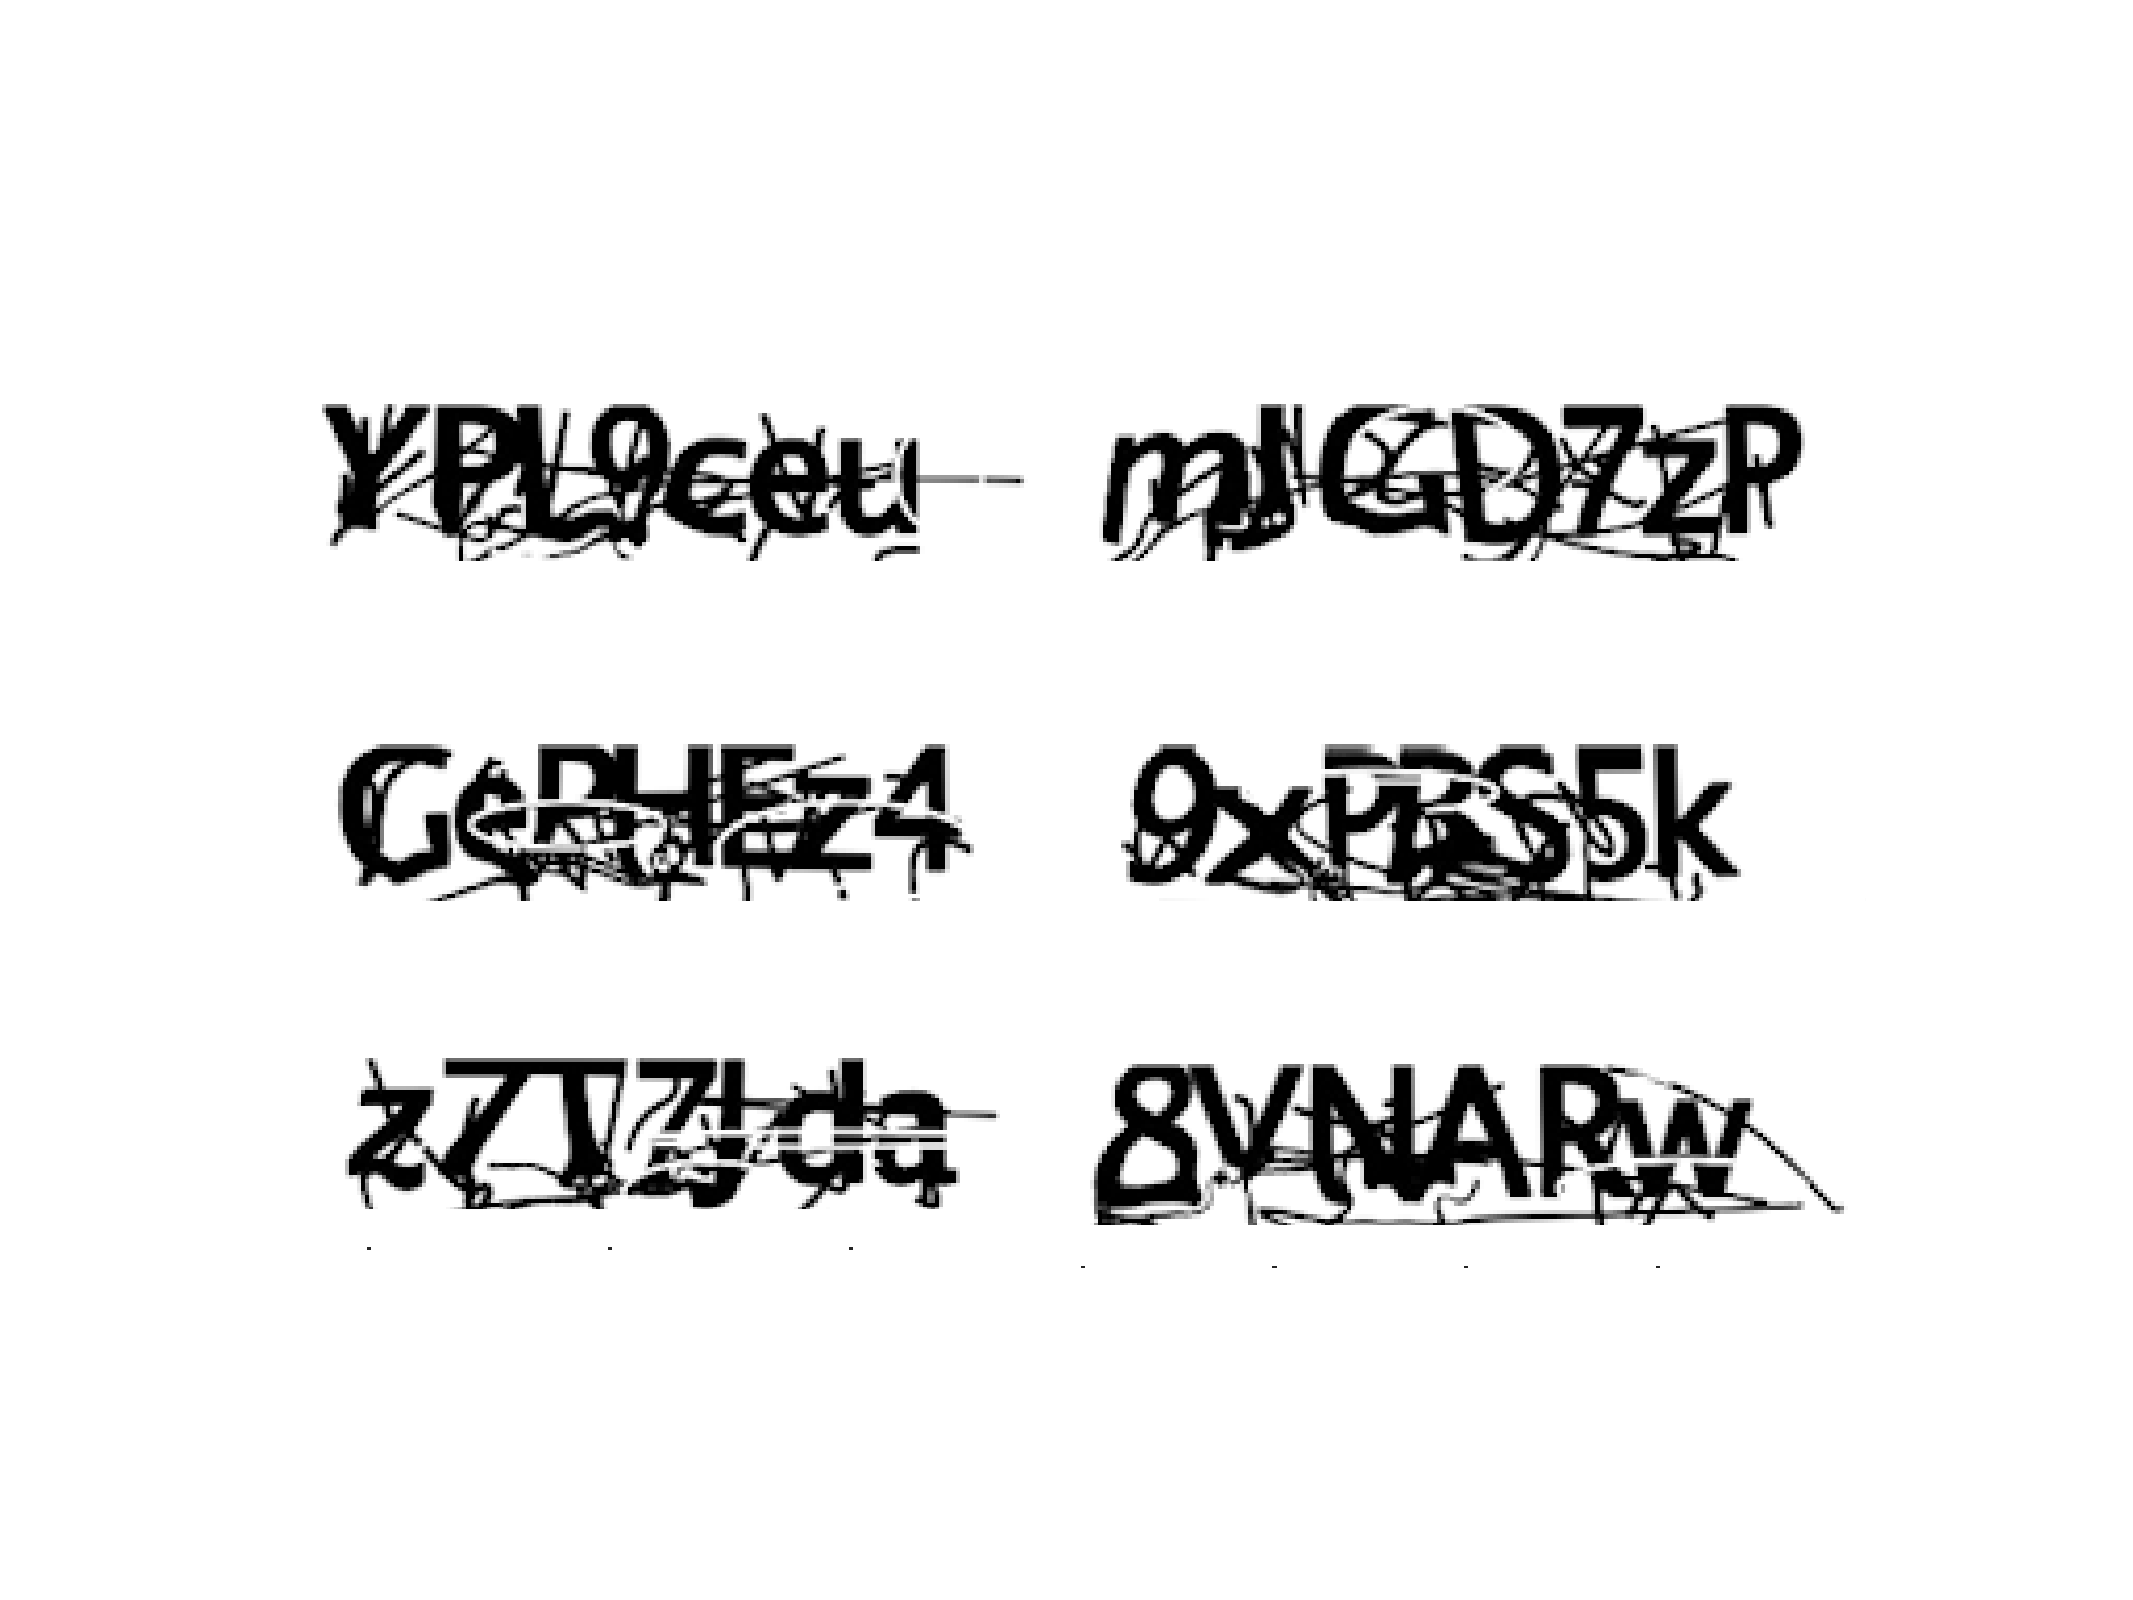
\includegraphics[width=\textwidth]{probprog/figures/example_captchas.pdf}
		\caption{Examples of real Captchas
			 \label{fig:probprog:example_captchas}}
	\end{subfigure}
	~~
	\begin{subfigure}[t]{0.38\textwidth}
		\centering
			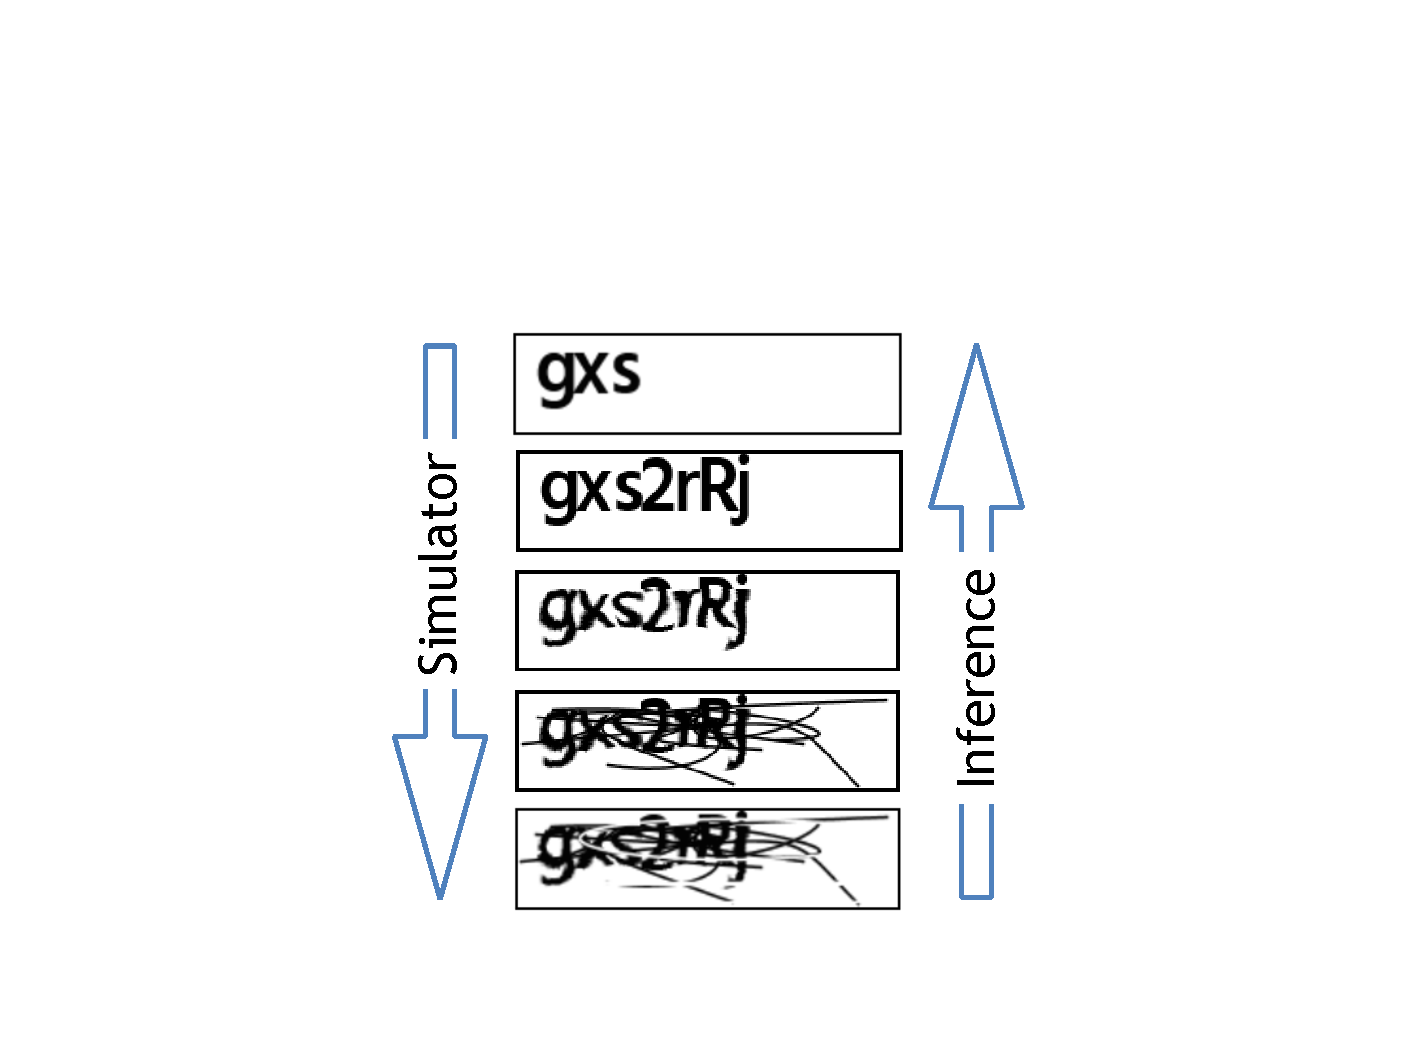
\includegraphics[width=\textwidth]{probprog/figures/captcha_sim.pdf}
		\caption{Example simulation of a Captcha
			\label{fig:probprog:captcha_sim}}
	\end{subfigure}
	\vspace{5pt}
	\caption{Solving Captchas by simulator inversion.   \textbf{(a)} gives examples of real
		Facebook Captchas taken from~\cite{le2017using}.  Here the corresponding
		generating strings going
		to clockwise from the top left are YPL9ceu, mJGD7zP, 9xPBS5k, 8VNARw, z7T7Jda, and
		GePHEz4.  A user is asked to type in these strings when shown the corresponding
		image to show they are not a robot.
		\textbf{(b)} gives an example of the process of simulating Captchas taken by
		~\cite{le2017inference}.  Here we see that we can generate a Captcha by first
		simulating a series of characters, then simulating appropriate manipulations 
		to those characters such as warping, rotating, and adding noise.  Inverting this
		simulation process corresponds to an inference problem, where we want to find
		out the characters that lead to a particular image.
		\label{fig:probprog:captcha}}
\end{figure}

Doing this process in reverse, i.e. simulating a Captcha, on the other hand, is a substantially
less daunting process.  The true Captchas are actually generated by
a simulator and so we can attempt to mimic this original simulation process.
For example, as shown in Figure~\ref{fig:probprog:captcha_sim} we might first sample a 
number of characters, then a symbol for each character, apply manipulations such as rotations and warpings, simulate
some obscuring lines or other noise, and finally render our simulated components into an
image.  Though admittedly it might take some time and effort to construct a high fidelity
simulator that well matches the produced images, the technical requirements for doing this
(other than possibly the final rendering) are minimal and so it could be carried out by most
people with a reasonable degree of experience in scientific programming.  The number of
people able to write such a simulator should certainly be substantially larger than the
number of people with sufficient experience in Bayesian modeling to construct an equivalent
graphical model or direct mathematical formulation.  The number of people
with the expertise to then write an appropriate inference scheme for the problem is even
smaller.  In a PPS, writing this simulator and providing the data is all that is required.
Given these, the PPS will carry out the inference required to invert the simulator automatically,
inferring the characters from the image.  More generally, we are estimating the inputs and
internal variables of our simulator, given target values for the outputs.

There are two key factors to realizing our aim of inverting simulators.  Firstly we need to provide a 
language which easily allows users to
write down simulators and which has semantics that allows the compiler to extract an appropriate
representation of the joint distribution.  In other words, we need our language to be sufficiently
general purpose and easy to use to not burden the user, while at the same time having syntax and semantics that
ensure the corresponding joint distribution is well defined and can be converted into a form where
we can run inference.  Doing this will require the introduction of means for \emph{conditioning} on data
and of specially defined \emph{random primitives} whose behavior can be controlled at 
run time, rather than just always sampling from
the same predefined distribution as they would in an ordinary programming language.  
The latter can be thought of as defining terms in the prior and the
former as terms in the likelihood as we will discuss in Section~\ref{sec:probprog:models}.
For certain cases, one can alternatively think of conditioning as applying \emph{constraints} to the
program.  For example, we can think of a probabilistic program as defining a simulator
and a set constraints that must be satisfied; this is exactly
how the PPS Church~\citep{goodman2008church} is designed.  An important distinction 
here though is between \emph{hard} and \emph{soft} conditioning.  Hard conditioning is as per the conventional
interpretation of a constraint -- we condition on the fact that an event occurs exactly.  Soft conditioning instead
assigns a weight to the program based on the probability (or probability density) of a given event occurring.
Though hard conditioning is a particular case of soft conditioning (for which the weight is either 1 or 0),
one can, at least semantically, use it to specify a soft conditioning, say 
$p(Y=y | X=x)$, by sampling $Y\sim p(y|X=x)$ and then imposing the constraint $Y=y$.
However, only supporting hard conditioning in a PPS is somewhat restrictive for practical
use, as one cannot effectively condition on continuous data because there is zero probability of
satisfying the resulting constraint.

The second key factor is that our language needs a general purpose inference(s)
engine capable of working on any program the user writes.  Bayesian models are fully defined
by their joint distribution and the data.  Therefore, once a user has written their simulator and provided
the data, this uniquely defines a posterior and the only problem is in solving the resulting Bayesian inference.
If we can now construct inference engines capable of working on arbitrary code, we can 
automate inference on any simulator or model the user defines, creating an
abstraction barrier between model definition and drawing inferences from that model.  We will discuss how this can be
done at length in Chapter~\ref{chp:proginf}.

If we can construct a system that can successfully carry out these tasks, 
the huge potential applications this could provide should be clear. We would have a 
system where the user requires no expertise in inference or conventional
Bayesian modeling in order to write application specific models and have them solved automatically.
Instead, they need only have the ability to write stochastic simulators for the process they wish to
model, a skill possessed my most of the scientific community and many of those outside it as well.
In a hypothetical future where scientists
code all their simulators in extremely powerful PPSs, tasks such as
inverting those simulators and improving the simulator by incorporating real data would
be automated in the same way current compilers convert high-level coding languages to machine code.  
However, this ability is not completely
hypothetical -- many such problems can already be handled by existing systems.  The challenge
is improving and scaling such systems to deal effectively with more difficult and more wide ranging models
in a tractable manner.  The need for such systems to work in an automated manner for a wide array
of possible problems makes this a very difficult problem; after all we are somewhat flaunting the no-free-lunch
theorem.  However, there is a key component that provides hope that this may be possible: we have access
to the target source code of the simulator itself, rather than needing to treat it as a black-box as is the
case for, say, approximate Bayesian computation (ABC) methods~\citep{csillery2010approximate}.  Therefore
maybe we can have our cake and eat it by using the source code itself to guide our algorithms, such that
they behave in problem specific ways.  We will discuss how this can be done at length in 
Chapters~\ref{chp:proginf} and~\ref{chp:bopp}.
% !TEX root = ../main.tex

\section{Differing Approaches}
\label{sec:probprog:two}

Rather than being a clearly defined method,
probabilistic programming is more of an umbrella term that covers a spectrum of 
different approaches, varying from inference toolboxes through to universal probabilistic programming
languages (PPLs) that allow
arbitrary probabilistic code to be written.
%, even that which might not correspond to a valid model.  
Often there is a trade-off between efficiency and expressivity: the more restricted
one makes the language, the more those restrictions can be exploited to improve the efficiency
of the inference.  This leads itself two distinct philosophies when developing a system. 
Firstly one can start with a particular inference algorithm and then design a system around making it as
easy as possible to write models for which that inference algorithm is suitable.  Secondly one can start
with  a general purpose PPL that allows as many model as possible to be written and then try to construct
inference engines that are capable of work in such a general framework.  Both approaches 
have their merits and drawbacks, with the distinction typically coming down to the intended use.
We will now elucidate each approach more precisely.  

\subsection{Inference Driven Systems}
\label{sec:probprog:two:inf}

Though there is a plethora of bespoke inference algorithms designed for particular models, the vast majority of these are based around
a relatively small number of foundational methods such as importance sampling, sequential Monte Carlo,
Metropolis-Hastings, Gibbs sampling, message passing, and variational inference (see Chapter~\ref{chp:inf}).
The extensive use of these core inference approaches throughout Bayesian statistics and machine
learning means that it makes clear sense to write packages for automating them and which
make it easy for the user to define an appropriate graphical models for which the inference can be automated.
This both improves efficiency of modeling and reduces barriers to effective Bayesian modeling by reducing the
required inference expertise for users.  This inference-first philosophy is taken by a number of successful PPSs
and inference toolboxes (the distinguishing line between which can be a little blurry), a small number of which we now 
briefly outline.

BUGS (Bayesian inference Using Gibbs Sampling) \citep{spiegelhalter1996bugs} and its 
	extensions~\citep{lunn2000winbugs,plummer2003jags,todeschini2014biips}
	allow finite DAGs to be specified using declarative code or pictorially using a graphical user
	interface.  These are converted to a form that is suitable for inference, the exact nature of which
	depends on the implementation, with the original work being based on Gibbs sampling.
	
Infer.Net \citep{minka_software_2010} is modeling language for defining, and automating approximate inference in
	both DAGs and Markov random fields, using predominantly message-passing algorithms. Distributions
	are generally, though not exclusively, restricted to be exponential families.  Branching (i.e. \texttt{if}) 
	is allowed, but requires enumeration of all possible paths at run time.

LibBi \citep{murray2013bayesian} is a package for doing Bayesian inference for state-space models,
	using particle-based inference methods (see Chapter~\ref{chp:part}).  It has a strong focus on scalable
	computation, providing support for multi-core architectures and graphics processing units.

PyMC3 \citep{salvatier2016probabilistic} is a python framework for carrying out MCMC and variational
	inference, using Theano~\citep{bergstra2010theano} to calculate the gradients required by some inference methods.

Stan \citep{carpenter2015stan} is a PPS with interfaces to many difference languages and a
	focus on performing Hamiltonian Monte Carlo inference~\citep{duane1987hybrid,hoffman2014no}, though
	other inference methods such as variational inference are also provided~\citep{kucukelbir2015automatic}.
	As with PyMC3, automatic differentiation is used to calculate required gradients.  The need to take
	derivatives means that there is limited support for discrete variables or branching.

These systems do not allow users to write models that would be difficult (at least for
an expert) to code without a PPS -- in general they all can be thought of as defining a graphical model
or sometimes factor graph -- but they offer substantial utility through ease of model exposition and
automating inference.

\subsection{Universal Probabilistic Programming}
\label{sec:probprog:two:general}

As useful as these inference-driven systems are, they do not fit very well with the notion of
inverting simulators we introduced in Section~\ref{sec:probprog:inv}.  They are still closely tied
to graphical models and are more toolboxes for streamlining the Bayesian modeling process than
a means of writing models that would be problematic to define by conventional means.  Achieving
our long term ambitious aim of making general purpose systems for conducting inference of
arbitrary simulators will require us to take a somewhat different approach that instead starts
with a general-purpose language and then attempts to design inference algorithms capable of
working on arbitrary models and code.  It will be necessary for such systems to
support models where the set of random variables is dynamically typed, such that it is possible 
to write programs in which this set, and thus potentially the number of random variables, differs 
from execution to execution.  To avoid hindering the user or restricting the models which can be
defined, it will important to allow 
things such as branching, recursion, higher-order functions,
conditional existence of variables, and arbitrary black-box
deterministic functions.  Ideally, we would like to provide no restrictions on the code that the user
can write, except for eliminating programs do not define valid probability distributions, such as
those that have a non-zero probability of never terminating.  In practice catching such invalid cases can
be hard or even impossible and so many systems actually adopt a philosophy of applying no restrictions,
such that it is perfectly possible to define invalid models.  General purpose PPSs actually bring up new
theoretical questions about what constitutes a valid probability model~\citep{heunen2017convenient}, while
even the set of valid definable models is a strict super-set of the those definable by graphical models 
for many systems~\citep{goodman2013principles}.

In the rest of this thesis, we will predominantly focus on these \emph{universal} PPLs~\citep{goodman_uai_2008,staton2016semantics}, 
so-called because they are based on \emph{Turing complete} languages that can specify any
computable distribution~\citep{goodman2013principles}.  For our purposes, we further refine this definition
to systems that also allow specification for any computable conditioning.
We will regularly using the universal PPL Anglican~\citep{wood2014new} as a reference, an introduction
to which is provided in Section~\ref{sec:probprog:anglican}. Here we will briefly discuss some other
prominent higher order PPLs.

Church is a PPL based on Scheme \citep{goodman_uai_2008}.  
The original seminal paper and accompanying system 
	forms a foundation on which many of the prominent existing systems are built through its
	demonstration that higher-order probabilistic programs define valid probability models, even in
	the presence of infinite recursion.  However, Church predominantly only allows hard
		conditioning,\footnote{Some very limited support for soft-conditioning is provided in current
		implementations through a ``noisy equals'' that equates to a Gaussian likelihood.}
	namely a model in Church comprises of a generative sampler and a separate predicate procedure
	which returns true if the desired conditions are satisfied.  
	In addition to the aforementioned issues of hard conditioning, this complete separation of the 
	generative process and the conditioning can also be wasteful in not allowing the structure of a 
	model to be exploited (see Chapters~\ref{chp:part} and \ref{chp:proginf}).  
	Later systems therefore mostly allow soft conditioning statements to be interleaved
	through the generative progress (in an analogous manner to likelihood terms), increasing the range
	of (solvable) models than can be encoded and the potential efficiency of inference algorithms.
	Inference in Church (and its direct derivatives) is typically carried out using either rejection sampling
	or MCMC.  Church places a particularly strong emphasis on the ability to carry out \emph{nested inference},
	something we will look into in depth in Chapter~\ref{chp:nest}.

Venture~\citep{mansinghka2014venture} is a probabilistic programming platform providing a flexible
system for both specification of models and inference methods.  In has a strong emphasis on being extensible
and for allowing the hosting of eternal applications.  For example, it allows the user to provide proposals for
the inference engine or reprogram the inference strategy entirely.  Venture is predominantly used via the
VentureScript~\citep{mansinghka2014venture} PPL.

WebPPL \citep{goodman_book_2014} is a PPL built using a purely functional subset of Javascript,
conveniently allowing for embedding in web pages.
In combines the ability to write a generative process using sampling statements and to add in likelihood
terms through a {\small \texttt{factor}} primitive that is analogous to the \observe primitive that we will introduce
in Section~\ref{sec:probprog:models:first}.  At its back end, WebPPL provides a number of different inference
algorithms, such as SMC and MCMC methods.

The price for the expressivity of these general purpose systems is a substantial extra 
burden on the inference engine as we will
discuss in Chapter~\ref{chp:proginf}.  In general, inference methods for such systems 
must be formulated in such a manner that they are applicable to models where the 
density function is intractable and can only be evaluated during forwards simulation of the program. 
For example, it may not be possible to know if a variable is continuous or discrete except by
running the program, while some variables will only exist conditioned on the values of others.
This required generality of the inference engine will naturally lead to a drop in performance compared to
custom written inference code, but this is often a price worth paying for generality and automation, particularly
when considering models that would be challenging to express, let alone do inference in, using more
conventional frameworks.
% !TEX root = ../main.tex

\section{Bayesian Models as Program Code}
\label{sec:probprog:models}

In the last section we shown how we can thing of PPS as inverting simulators, predicting internal
variables and the inputs given the outputs.  In this section we will take a different perspective and
show how we can translate Bayesian modeling into the framework of program code.  As we 
showed in Chapter~\ref{chp:bayes} we showed how a Bayesian model is defined by a prior over
parameters and a likelihood function for those parameters given the data.  This viewpoint will
mostly translate into the probabilistic programming setting by equating between the prior
and sampling statements and between the likelihood and conditioning statements.  At the end
of the section we will explain why this is actually a slight approximation (in short because we
might condition on internally sampled variables) but for most purposes this viewpoint will suffice.
We will keep things predominantly high-level for now, giving a more detailed look in
Section~\ref{sec:probprog:anglican} by introducing a particular PPS, namely Anglican, in detail.

\subsection{A Simplified Probabilistic Programming Setup}
\label{sec:probprog:models:first}

We start by considering the case of constructing a restricted PPS.  We will presume that our
language has no branching (i.e. no \texttt{if} statements or equivalent), is  first order
(i.e. variables cannot be functions), that there is no recursion, and that it does not allow 
any conditioning on internally sampled variables.  
We will give our language
two special constructs, \sample and \observe, between which the distribution of the
program is defined.  As such the program should not include any other random components.
Informally, \sample will be used to specify terms in the prior and \observe terms in the
likelihood.  More precisely, \sample will be used to make random draws $x_t \sim f_t(x_t | \Xi_t)$,
where $\Xi_t$ is a subset the other variables in scope at the point of sampling, and \observe will use to condition on
data $g_s(y_s|\Lambda_s)$ with $\Lambda_s$ defined in the same way as $\Xi_t$.  We presume that the program takes 
in as input external parameters $\theta$ and data $y_{1:S}$, the former of which is taken as inputs that are 
not ``observed'' at any point but can effect the conditioning through $\Xi_t$ and $\Lambda_s$, while we presume 
for our simplified setup that the latter appears in neither $\Xi_t$ or $\Lambda_s$.
We define both \sample and \observe as adding a factor to the joint distribution which is therefore given by
\begin{align}
\label{eq:probprog:simple-joint}
p(x_{1:T},y_{1:S} | \theta) = \prod_{t=1}^{T} f_t(x_t | \Xi_t) \prod_{s=1}^{S} g_s(y_s|\Lambda_s).
\end{align}
The two vary in whether they define a new random variable or effect the probability of the
program given particular instances of the other random variables.
Our presumptions for this simplified setup that no $y_{s}$ terms are present in the $\Xi_t$ or $\Lambda_s$
and that we do not condition on internally sampled variables, means that we can here have
exactly that our prior is $\prod_{t=1}^{T} g_t(x_t | \Xi_t) =: p(x_{1:T} | \theta)$ and our likelihood is
$\prod_{s=1}^{S} g_s(y_s|\Lambda_s) =: p(y_{1:S} | x_{1:T}, \theta)$.  Consequently, for our simplified setup,
each program defines a finite directed acyclic graphical model (see Section~\ref{sec:bayes:paradigm:graph})
where the conditional relationships are defined through the definitions of $f_t$ and $g_s$.
This breakdown into a prior and likelihood and the equivalence to graphical models
will not hold in the more general cases we consider later.  \todo[inline]{Some example programs and equivalent
	graphical models for our simplified setup are given in Figure INSERT}

An important point to note is that~\eqref{eq:probprog:simple-joint} shows that all of our \sample
and \observe statements are exchangeable, in the sense that their order can be moved around and
still define the same joint distribution, up to restrictions about all the required variables required
for the conditioning existing and being in scope.  For example, if all variables remain in scope
and are not redefined, we can generally move all our \observe statements to the end of the program
without changing the joint distribution.  Nonetheless, the position of the \observe statements
can often be important from the perspective of the performance of the inference engine.  This exchangeability
result will carry over to the non-simplified cases.

Other than \sample and \observe statements, the rest of our program is by construction totally deterministic.  Therefore,
though it may contain random variables other than $x_{1:T}$, these random variables are deterministic
functions of the ``raw'' random draws $x_{1:T}$ and inputs $\theta$ and $y_{1:S}$.  We can therefore 
define the outputs of our program as $z := h(x_{1:T},y_{1:S},\theta)$ for some deterministic function $h$.
As we explained in Section~\ref{sec:prob:measure}, the change of variables means that the density function on $z$,
$p(z | y_{1:S}, \theta) $
can have a different form to the posterior implied by our program, namely $p(x_{1:T} | y_{1:S}, \theta)$.
  Though this is a serious complication in the
context of optimization (we may not in general be able to find $\argmax_z p(z|y_{1:S},\theta)$
or even evaluate $p(z | y_{1:S}, \theta)$ exactly), it
is perfectly acceptable in the context of calculating expectations as
\begin{align}
\int f(z) p(z | y_{1:S}, \theta) dz = \int f(h(x_{1:T}, y_{1:S}, \theta)) p(x_{1:T} | y_{1:S}, \theta) dx_{1:T}
\end{align}
for implicitly defined measures $dz$ and $dx_{1:T}$.  Two consequences of this are that
we can express any expectations calculated by our program as expectations over $p(x_{1:T} | y_{1:S}, \theta)$
which was fully defined by the joint~\eqref{eq:probprog:simple-joint} and that, provided we are not worried
about carrying out optimizations, we do not need to explicitly worry about the implicit measures defined
by the definition of our program, other than any potential effects on the inference scheme.


%
%Because of the assumptions we have made for our language, the latent
%variables we wish to do inference for are statically determined as $x_{1:T} = x_1,\dots,x_T$ 
%such that the posterior of interest is $p_{\theta} (x_{1:T} | y_{1:S})$ (or some marginal of this for
%which we can still using Monte Carlo inference on the joint).
%
%Our implied target posterior
%is proportional to this joint in the standard way $p_{\theta}(x_{1:T}|y_{1:S}) \propto p_{\theta}(x_{1:T},y_{1:S})$.

\subsection{A General Probabilistic Programming Setup}
\label{sec:probprog:models:general}

Note that as $y_s$ terms can appear in the $\Xi_t$ terms, it can be the case that 
$p(x_{1:T} | \theta) \neq \prod_{t=1}^{T} p(x_t | \Xi_t)$ such that the latter does not
ex
can also enter \sample or \observe terms through $\Xi_t$ and $\Xi_s$ respectively.

\todo[inline]{Conditioning on internally sampled variables
	
	Ordering of decelerations matters
	
	Memoization
	
	Complications of maximization}
% !TEX root = ../main.tex

\section{The Anglican Probabilistic Programming Language}
\label{sec:probprog:anglican}

To allow for a more precise consideration of issues associated with designing and using a universal
PPS, we now introduce the particular language \emph{Anglican}~\citep{wood2014new,tolpin2016design},
which we will use for reference throughout the rest of the thesis.  
Anglican is a universal PPL integrated into \emph{Clojure}~\citep{hickey2008clojure}, a dynamically-typed, general-purpose, functional
programming language (specifically a dialect of Lisp) that runs on the Java virtual machine and uses just-in-time compilation.
Anglican inherits most of the syntax of Clojure, but extends it with the key
special forms \sample and \observe \citep{tolpin2015probabilistic,tolpin2016design}, defined in the same way as
our example language setup in the previous section, along with a couple of others which aid in defining queries
such as \mem, \store, and \retrieve.  Despite using predominantly the same syntax, Anglican has different, 
probabilistic, semantics to Clojure, i.e. code is written in the same way, but is interpreted differently.

Anglican was the first PPL to introduce particle based 
inference schemes such as SMC and particle MCMC (see Chapters~\ref{chp:part} and \ref{chp:proginf}), which was
key advancement for universal PPSs because it allows the structure of the query to be exploited to provide
substantially more efficient inference then previous approaches.  Though these methods still form the core
of the inference in Anglican, there have been a number of advancements and alternative inference approaches introduced since
the original work~\citep{paige2014asynchronous,tolpin-socs-2015,tolpin2015output,vandemeent_aistats_2015,
	rainforth2016interacting,rainforth2016bayesian,le2017inference}.  Another notable feature of Anglican is its
support for Bayesian non-parametric modeling, such as providing support for general processes along with
primitives for particular models such as Dirichlet processes.  Inevitably we can only provide a limited 
introduction here and so we also refer the interested reader to~\cite{tolpin2016design} and to the Anglican website {\small\url{http://www.robots.ox.ac.uk/~fwood/anglican/}} for more information.

\subsection{Clojure}
\label{sec:probprog:anglican:clojure} 

Before getting into the details of Anglican, we first give a very brief introduction to Clojure~\citep{hickey2008clojure},
because its syntax may be quite unfamiliar to readers without experience in Lisp based notation or functional programming
more generally.  There are two key things to get your head around for reading and using Clojure (and Lisp languages more
generally): almost everything is a function and brackets evaluate functions.  For example, to code $a+b$ in Clojure one
would write {\small \lsi{(+ a b)}} where $+$ is a function taking two arguments (here $a$ and $b$) and the brackets cause the
function to evaluate.  More generally, Clojure uses prefix notation such that 
the first term in a bracket is always a function, with the other terms the arguments.
Thus {\small \lsi{((+ a b))}} would be invalid syntax as the result of {\small \lsi{(+ a b)}}  is not a function so cannot be evaluated.
Expressions are nested in a tree structure so to code $2(a+b)/c$ one would write {\small \lsi{(/ (* 2 (+ a b)) c)}} .  One can
thus think about goes outwards in terms of execution order -- a function first evaluates its arguments before
itself.  Functions in Clojure are first class (i.e. they can be variables) and can be declared either anonymously using
{\small \lsi{(fn [args] body)}}, for example {\small \lsi{((fn [a b] (/ a b)) 10 5)}} evaluates to 2, or using the
macro \defn to declare a named function in the namespace, for example {\small \lsi{(defn divide [a b] (/ a b))}}.
Local bindings in closure are defined using \cllet blocks which are used to denote a number of name value
pairs, with the bindings persisting to closure defined by the brackets of the \cllet block and the return value
being the output of the last element in the \cllet block list.  Thus for example
{\small \lsi{(let [a 2 b 3] (+ a b))}} says let $a$ be equal to $2$, $b$ be equal to $3$, and then evaluate $a+b$, thus
returning $5$.  Note that $a$ and $b$ remain undefined outside of this let block.  

Clojure allows various types of compound literals such as vectors, lists, hash maps and sets.
In general, elements in these compound literals are not restricted in
there type so it valid to write for example {\small \lsi{[1 "2" (fn [x] (inc x))]}} to construct a vector 
whose component terms are different types.

Clojure does not generally use
for loops, instead relying the constructs \map and \reduce, or the \clj{loop}-\clj{recur} pairing.
\map applies a function to every value in a list or vector so for example {\small \lsi{(map (fn [a] (* a 2)) [2.1 3])}}
doubles each value in the vector of inputs returning a list {\small \lsi{(4.2 6)}}, where the brackets in the output
now just represent a list rather than a function evaluation, just to be be confusing.  \reduce recursively applies
a function and so for example to sum up a vector of elements in Clojure one writes for example
{\small \lsi{(reduce + 0 [1.2 3.4 2])}} which returns $6.6$.  The \clj{loop}-\clj{recur} pairing forms
a syntax sugar for doing looping through tail recursion.  In essence, \clj{loop} defines a function and provides
initial bindings for the input arguments.  Inside the \clj{loop} function block, \clj{recur} recursively calls the
function defined by \clj{loop} with new bindings to the inputs.  In general, the \clj{recur} function should
only be called depending on a condition holding true to prevent infinite recursion.  To give a concrete example,
 \begin{lstlisting}[basicstyle=\ttfamily\small,frame=none]
 (loop [x 1] (if (> x 10) nil (do (print x) (recur (+ x 1)))))
 \end{lstlisting}\vspace{-5pt}
will print out the numbers $1$ to $10$.  Here the syntax of \clj{if} is \clj{(if test then else)} so when \clj{x>10}
it returns \clj{nil}.  Otherwise it calls the \clj{do} statement which evaluates each of its arguments in turn, in
this case printing out $x$ before recalling the body of the \clj{loop} block with \clj{x}  reset to \clj{(+ x 1)}.

A important feature of Clojure, particularly with regards to Anglican, is its support for (infinite) lazy sequences.
Lazy sequences are sequences of terms that are only evaluated as an when they are required.  As such, it is 
valid for them to be infinitely long (typically through recursive definition) because terms are only calculated if
they are required, so it is possible to define a term that is theoretically infinite long, but only a finite number
of values from which are ever evaluated in practice.    For example one can define the function
 {\small \lsi{(defn ints [n] (lazy-seq (cons n (ints (inc n))))}} and then call {\small \lsi{(ints 1)}} to produce a
lazy sequence comprising of all the positive integers.  We can evaluate the sequence by explicitly requesting
terms with the sequence.  For example, we can use {\small \lsi{(take 5 (ints 1))}} to return the first $5$ elements
of our lazy sequence, thus returning {\small \lsi{(1 2 3 4 5)}}.  We could also ask for a particular term in the
sequence using, for example, {\small \lsi{(nth 4 (ints 1))}} to return $5$.
Lazy sequences are conceptually useful, amongst other things, for specifying things that
are required to be infinitely long to ensure theoretical guarantees (engine an MCMC sampler needs to be run
infinitely long to converge), but which are restricted by computational budgets.

\subsection{Writing Models in Anglican}
\label{sec:probprog:anglican:models} 

Anglican queries are written using the macro \defquery.  This allows uses to the define a model using a mixture
of \sample and \observe statements and deterministic code in the manner synonymous to that explained in
Section~\ref{sec:probprog:models}, and bind that model to a variable.  
As before, Anglican makes use of distribution objects for providing inputs to \sample and \observe, for which
it provides a number of common constructors corresponding to common
elementary random procedures such
as \gammaa, \normal, and \betaa.  A distribution objects is generated by calling the class constructor
with the required parameters, e.g. {\small \lsi{(normal 0 1)}} for the unit Gaussian.
Anglican also allows custom distribution classes to be defined using
the \defdist macro, which requires the user to provide parameterized code for sampling from that distribution
class and evaluating the log density at given output.

\begin{wrapfigure}{r}{0.5\textwidth}
	\centering 
	\begin{lstlisting}[basicstyle=\ttfamily\small]
(defquery my-query [data]
  (let [mu (sample (normal 0 1))
        sig (sample (gamma 2 2))
        lik (normal mu sig)]
   (map (fn [obs]
          (observe lik obs))
     data)
  [mu sig]))
	\end{lstlisting}	
	\vspace{-5pt}
	\caption{A simple Anglican query.\label{fig:probprog:simple-ang}}
	\vspace{-10pt}
\end{wrapfigure}
A simple example of an Anglican query is shown in Figure~\ref{fig:probprog:simple-ang},
corresponding to a model were we are trying to infer the mean and standard deviation
of a Gaussian given some data.  The syntax of \defquery is {\small \lsi{(defquery name [args] body)}}
so in Figure\ref{fig:probprog:simple-ang} our query is named {\small \lsi{my-query}} and takes
in arguments {\small \lsi{data}}.  The query starts by sampling {\small \lsi{mu}}$\sim\mathcal{N}(0,1)$
and {\small \lsi{sig}}$\sim\textsc{Gamma}(2,2)$ and constructing a distribution object {\small \lsi{lik}}
to use for the observations.  It then maps over each datapoint and observes it under the distribution
{\small \lsi{lik}}, remembering that {\small \lsi{fn}} defines a function and \map applies a function
to every element of a list of vector.  
Note that \observe simply returns {\small \lsi{nil}} and so we
are not interested in these outputs -- they effect the probability of a program execution trace, but
not the calculation of a trace itself.  After the observations are made, {\small \lsi{mu}} and {\small \lsi{sig}}
are returned from the \cllet block and then by proxy the query itself.
Because the data terms only get used as observations and we do
not observe any internal random variables, this query corresponds exactly to a Bayesian model where
the \sample terms form the prior and the \observe terms form the likelihood as we explained in
Section~\ref{sec:probprog:models:general}.  The query thus defines a correctly normalied joint
distribution given by
\begin{align}
p(\mu,\sigma,y_{1:S}) = \mathcal{N}(\mu ; 0,1) \; \textsc{Gamma}(\sigma ; 2, 2) \prod_{s=1}^{S} \mathcal{N}(y_s ; \mu, \sigma)
\end{align}
where we have defined $\mu:=${\small \lsi{mu}}, $sig:=${\small \lsi{sig}}, and $y_{1:S}:=${\small \lsi{data}}.
Other more complicated example Anglican models are given in Figures~\ref{fig:probprog:example-ang}
and~\ref{fig:probprog:schell}.

\begin{figure}[t]
	\centering
	\begin{subfigure}[t]{0.45\textwidth}
			\centering	
\begin{lstlisting}[basicstyle=\ttfamily\footnotesize]
(defquery lin-reg [xs ys]
 (let [m (sample (normal 0 10))  
       c (sample (normal 0 3))
       s (sample (gamma (1 1)))
       f (fn [x] (+ (* m x) c))]
  (map (fn [x y]
    (observe 
      (normal (f x) s) y))
   xs ys)
 [m c s])
\end{lstlisting}				
			\caption{Linear regression model with unknown
				observation variance.  Here \clj{xs} and
	 \clj{ys} are the data comprising of the inputs and corresponding
	 outputs of the regression.  The query returns estimates
	 for the slope \clj{m}, the intercept \clj{c}, and the observation
	 standard deviation (i.e. noise) \clj{s}. \label{fig:probprog:lregang}
		}
	\end{subfigure}
~~
	\begin{subfigure}[t]{0.52\textwidth}
		\centering	
\begin{lstlisting}[basicstyle=\ttfamily\footnotesize]
(defquery discrete-hmm
 [ys x0 trans obs]
 (loop [xs x0 t 0]
  (let 
   [x (sample (nth trans (last xs)))]
   (observe (nth obs x) 
     (nth ys t))
   (if (= (inc t) (count ys))
    (conj xs x)
    (recur (conj xs x) (inc t))))))
\end{lstlisting}	
		\caption{Hidden Markov model with discrete states.
	Here \clj{ys} is the data, \clj{x0} is a starting state (which
	has no associated observation), \clj{trans} is the collection of 
	transition distribution objects for each of the $K$ possible states
	(index by the value of $x_t$), and \clj{obs} are the matching
	emission distributions.	Query returns
	estimates for the latent states \clj{xs}.\label{fig:probprog:hmm}
		 }
	\end{subfigure}
		\caption{Example Anglican queries for some simple models. Here \defquery
			binds a query to a variable, for which inference can be run using \doquery. 
			with syntax
			{\footnotesize \lsi{(doquery inf-alg model inputs & options)}}. 
			For example, we could call {\footnotesize \lsi{(doquery :ipmcmc
					lin-reg [xs ys] :number-of-particles 1000)}}  for some
			predefined \lsi{xs} and \lsi{ys} to run iPMCMC inference (see Section~\ref{sec:part:ipmcmc}))
			on the \lsi{lin-reg} model with with 1000 particles.
			\label{fig:probprog:example-ang}}
\end{figure}

Compilation of an Anglican program is performed by the macro \query.  Calling \query
invokes a source-to-source compilation from an Anglican query to a continuation-passing 
style (CPS) Clojure function that can be executed using a particular inference algorithm.  We
leave discussing what this means in depth to Chapter~\ref{chp:proginf}, noting only that
the inference algorithms associated with Anglican are written in pure Clojure (except for the odd
bit of Java code) and the aim of the compilation is to product a model artifact which can be
interpreted by that inference code.
When \defquery is called, Anglican internally calls the \query and assigns the output to
the symbol provided by the first argument of \defquery.  Therefore {\small \lsi{my-query}} in
our example is Clojure function that can be read by the Anglican inference engines to produce
approximate samples from the conditional distribution.  Note that, as a Clojure function, the
inputs and body of {\small \lsi{my-query}} and not as per lexical definition of the Anglican program
(e.g. in now takes multiple inputs).  It is instead a function that encodes all the information 
required by the inference engine to perform inference and has the corresponding required call structure
for the input required by the engine.

\begin{figure}[p]
		\centering	
		\vspace{-20pt}		
\rule{\linewidth}{0.4pt}
\vspace{-28pt}		
		\begin{lstlisting}[basicstyle=\ttfamily\footnotesize,multicols=2,frame=none]
(defdist strike [volatility] []
 (sample* [this] 
   (if (sample* (flip volatility)) 
        :war :peace))
 (observe* [this value] 
  (observe* (flip volatility) 
    (= value :war))))
  
(declare A B)

(with-primitive-procedures [strike]
 (defm A [depth]
  (let [B-strike (B (dec depth))
        A-strike (strike 0.1)]
   (observe A-strike B-strike)
   B-strike))
   
 (defm B [depth]
  (let [B-strike (strike 0.2)]
   (if (> depth 0)
    (let [A-strike (A depth)]
     (observe B-strike A-strike)
     A-strike)
   (sample B-strike))))

 (defquery war [depth]
   (or (= (A depth) :war)
       (= (B depth) :war))))
\end{lstlisting}	
\vspace{-20pt}		
\rule{\linewidth}{0.4pt}
%\vspace{5pt}
		\caption{Anglican code for an example Schelling co-ordination game~\citep{schelling1980strategy,stuhlmuller2014reasoning}
		modeling if a peace will hold between two volatile countries which we refer to as A and B.
		This example is adapted from an online Anglican example developed by Brooks Paige and Frank Wood
		which can be found at~\url{http://www.robots.ox.ac.uk/~fwood/anglican/examples/}, providing a more
		detailed consideration along with other examples.
		Our code first defines a custom distribution called \lsi{strike} for modeling whether one country will
		attack the other if it does not reason about the other's actions.  
It then constructs a Anglican function for each country using \defm.  
Each country has their own volatility and the ability to reason about whether they think the other country will
initiate a strike against them. We presume they have access to the exact model of the other country.  A's aim is to match
the action it thinks B will do -- it would prefer there to be no war, but if there is, it wants to strike
first.  Its model first samples a draw for B's action by simulating from B's model and then observes this action
under its own distribution on whether to strike; this is equivalent to sampling both in isolation and constraining
them to be the same.  However, B can also reason about A and
A knows it.  It therefore provides the simulation of B's model with a \emph{meta-reasoning depth}.  If this depth
is zero, B makes its decision in isolation, simply sampling from \lsi{B-strike}.  If the depth is greater 
than zero though, it uses the same approach as A, simulating from A's model (with a depreciated meta-reasoning 
depth) and then observing this 
outcome under \lsi{B-strike}.  This creates a mutually recursive cycle of reasoning.  As an observer, we are
interested in establishing the probability that one of the two will strike, as this event leads to a war,
and so we define a query which outputs whether the two are the same.
The expectation of the output from this query corresponds to the probability of war.
Invoking inference using \lsi{(doquery :lmh war [depth])} we see that for a depth of $0$, there
is roughly a $0.222$ chance of war, while depths of $1$, $2$, and $10$ give rough respective chances of $0.052$, $0.0021$,
and $3\times10^-6$.  Thus the chance of war goes down the more each country thinks about the reasoning
of the other.  It is interesting to note that if the volatilities are set to the same value then
the critical tipping point, above which things escalate towards war with increased depth, is around $0.38$.
The mutual recursion involved in the model and the fact that variables are both sampled and 
observed means that it would be difficult to encode it using a graphical model.  It is not even clear how
one would go about writing down a well defined joint distribution for the model, without having to empirically
calculate a normalization constant.  Note though that this not correspond to a nested query example in the
manner we discuss in Section XX as there is no inference going on between the nested function calls.
\label{fig:probprog:schell}
		}
\end{figure}

Inference on the model is performed using the macro \doquery, which produces a lazy infinite sequence of 
approximate samples from the conditional distribution and, for appropriate inference algorithms,
an estimate of the partition function.
The syntax of \doquery is {\small \lsi{(doquery inf-alg model inputs & options)}} where {\small \lsi{inf-alg}}
specifies an inference algorithm, e.g. {\small \lsi{:ipmcmc}}, {\small \lsi{model}} is our query, {\small \lsi{inputs}}
is a vector if inputs to the query, the \& represents that there might be multiple additional inputs, and {\small \lsi{options}}
are is a series of option-value pairs for the inference engine.  For example, to produce 100 samples from
our {\small \lsi{my-query}} model with data {\small \lsi{[2.1 5.2 1.1]}} using the LMH inference algorithm with no
additional options, we can write {\small \lsi{(take 100 (doquery :lmh my-query [2.1 5.2 1.1]))}}.

Although Anglican mostly inherits Clojure syntax, some complications arise from the compilation to
CPS-style Clojure functions.  It is thus not possible to na\"{i}vely use all Clojure functions inside Anglican
without providing appropriate information to the compiler to perform the required transformation.
The transformation for many core Clojure functions has been code manually such that they form
part of the Anglican syntax and can be used directly.  Anglican further allows users to write functions externally
to \defquery using the macro \defm, which is analogous to \defn in Clojure and has the same call syntax (except
for being restricted input, though as this can be a vector, this places no restrictions on the functions that can be
written), which can then be called from inside the query without restrictions.  Other deterministic Clojure functions can also
be called from inside queries, but must be provided with appropriate wrapping to assist the compiler.  Thankfully
this is done automatically (except when the function itself is higher order) using the macro
{\small \lsi{with-primitive-procedures}} that takes as inputs Clojure functions and creates an environment where
these functions have been converted to their appropriate CPS forms.

We finish our introduction by noting the ability of Anglican to \emph{nest} queries within one another.  This
is somewhat experimental and comes with a number of health warnings because, as we will explain in Chapter~\ref{chp:nest},
it allows users to write so called \emph{nested estimation} problems that fall beyond the scope of the standard
proofs of convergence for stand Monte Carlo estimation schemes. Nonetheless, there are problems that cannot
be encoded without this ability, such as the Bayesian experimental design equations discussed in Chapter~\ref{chp:design}.
Though \doquery is not allowed directly within a \defquery block, one can still nest queries by 
either using a \doquery in a Clojure function that is then passed to another query using {\small \lsi{with-primitive-procedures}},
using a \doquery within a custom distribution defined by \defdist, or using the special form \conditional which
takes a query and returns a distribution object constructor, for which the inputs to the query become the parameters.
We will return to consider the implications of this at length in Chapter~\ref{chp:nest}.

%
%\section{Going Beyond Bayesian Inference}
%\label{sec:probprog:limit}

\todo[inline]{Memoization?}

\todo[inline]{
Interpreters rather than custom languages

Avoiding bugs in code}
% !TEX root = ../main.tex

\chapter{Inference}
\label{sec:inf}

\section{The Challenge of Bayesian Inference}
\label{sec:inf:challenge}

In the previous chapter we introduced the concept of Bayesian modelling and showed how we
can combine prior information $p(x)$ and a likelihood model $p(y|x)$ using Bayes' rule,
i.e.~\eqref{eq:bayes}, to produce a posterior $p(x|y)$ that
characterizes both our prior information and information from data.  We now consider the
problem of how to calculate (or more typically approximate) this posterior, a process 
known as Bayesian \emph{inference}.
At first this may seem like a straight forward problem: by Bayes' rule we have that
$p(x|y)\propto p(y|x)p(x)$ and so we already know the relative probability of any one
value of $x$ compared to another.  In practice this could hardly be further from the
truth.  Bayesian inference for the general class of graphical models is in fact an 
NP-hard problem \citep{cooper1990computational,dagum1993approximating}.  There are two
challenges in Bayesian inference: calculating the normalization constant
$p(y) = \int p(y|x)p(x)dx$ and providing a useful characterization of the posterior, for
example an object we can draw samples from.  Many inference schemes, for example Markov
chain Monte Carlo (MCMC) \citep{hastings1970monte}, will not
try to tackle these problems directly and instead look to generate samples directly from 
the posterior.  However, this breakdown will still prove useful in illustrating the challenges
presented by inference.

Calculating the normalization constant in Bayesian inference is essentially a problem of
integration.  Our target, $p(y)$, is the expectation of the likelihood under the prior,
hence the name \emph{marginal likelihood}.  When $p(y)$ is known, the posterior can be evaluated
exactly at any possible input point using~\eqref{eq:bayes} directly.  In the discrete case,
where our posterior represents explicit probabilities rather than a density function, the importance
of the normalizing constant is particularly plain to see.  When it is known then we can evaluate
the probability of any $x$ directly.  When it is not, then we have no concept of what might have been
missed.  Imagine a model where $x \in \{1,2,3\}$ with a corresponding uniform prior $P(x) = 1/3$
for each $x$.  Now imagine for some reason that we are only able to evaluate the likelihood at 
$x=1$ and $x=2$, giving $p(y|x=1)=1$ and $p(y|x=2)=10$ respectively.  Depending on the marginal
likelihood $p(y)$, the posterior probability of $P(x=2 | y)$ will vary wildly.  For example,
$p(y)=4$ gives $P(x=2 | y) = 5/6$, while $p(y)=1000$ gives $P(x=2 | y) = 1/100$.  Though this
example may seem far-fetched this is the scenario almost always seen in practice for realistic
models, at least all those with non-trivial solutions.  A common scenario is that it is not
possible to enumerate all the possible values of $x$ in reasonable time and we are left 
wondering - what is left?  The problem is even worse in the setting where $x$ is continuous, for
which it is naturally impossible to evaluate all possible values for $x$.  This problem is why
knowing the posterior only up to a normalization constant is deceptively unhelpful - we never
know how much of the probability mass we have missed and therefore whether the probability (or
probability density) where we have looked so far is tiny compared to some other dominant region
we are yet to explore.  At its heart, the problem of Bayesian inference is effectively the problem
about where to concentrate our finite computational resources so that we can effectively characterize
the posterior.  If $p(y)$ is known, then we immediately know whether we are looking in the right
place or whether we are yet to find where most of the posterior mass is hidden.  This brings us onto
our second challenge - knowing the posterior in closed form is often not enough!

\todo[inline]{Maybe talk about things in terms of the explore-exploit dilema a bit?}

% !TEX root = ../main.tex

\section{Particle Based Methods}
\label{sec:inf:smc}

We start by briefly reviewing sequential Monte Carlo \citep{gordon1993novel,doucet2001sequential} and the particle Gibbs algorithm \citep{andrieuDH2010}. Let us consider a non-Markovian latent variable model of the following form
\begin{subequations}
	\label{eq:ssm}
	\begin{alignat}{2}
		x_t | x_{1:t-1} &\sim f_t(x_t | x_{1:t-1}), \\
		y_t | x_{1:t} &\sim g_t(y_t|x_{1:t}),
	\end{alignat}
\end{subequations}
where $x_t \in \setX$ is the latent variable and $y_t \in \setY$ the observation at time step $t$, respectively,
with transition densities $f_t$ and observation densities $g_t$; $x_1$ is drawn from some initial distribution $\mu(\cdot)$. The method we propose is not restricted to the above model, it can in fact be applied to an arbitrary sequence of targets.

%We focus on the non-Markovian latent variable model because it has been shown to be useful within \eg probabilistic programming \citep{wood2014new}.%However, we restrict the exposition to the latent variable model for clarity and to see the potential usefulness of it to \eg probabilistic programming \citep{wood2014new}. \tom{I am not sure I agree with this statement - PP should actually allow the most general possible use of iPMCMC.  I think we would be better making the point that its ability to operate on arbitrary models make it a suitable candidate for PP inference engines.  By the final draft I would expect us to have it running and publically availible in Anglican}

We are interested in calculating expectations with respect to the posterior distribution $p(x_{1:T}|y_{1:T})$ on latent variables $x_{1:T} \eqdef (x_1,\ldots,x_T)$ conditioned on observations $y_{1:T} \eqdef (y_1,\ldots,y_T)$, which is proportional to the joint distribution $p(x_{1:T}, y_{1:T})$,
\begin{align}
	\label{eq:jointdistribution}
	p(x_{1:T} | y_{1:T}) \propto  \mu(x_1) \prod_{t=2}^T f_t(x_t | x_{1:t-1}) \prod_{t=1}^T g_t(y_t|x_{1:t}).\nonumber
\end{align}
In general, computing the posterior $p(x_{1:T}|y_{1:T})$ is intractable and we have to resort to approximations. We will in this paper focus on, and extend, the family of particle Markov chain Monte Carlo algorithms originally proposed by \citet{andrieuDH2010}. The key idea in \pmcmc is to use \smc to construct efficient proposals of the latent variables $x_{1:T}$ for an \mcmc sampler.

%
%   SMC
%

\begin{algorithm}[tb]
	\caption{Sequential Monte Carlo \hfill {\small (all for $i=1,\ldots,N$)}}
	\label{alg:smc}
	\begin{spacing}{1.2}
		\begin{algorithmic}[1]
			\STATE {\bfseries Input:} data $y_{1:T}$, number of particles $N$, proposals $q_t$
			\STATE $x_1^i \sim q_1(x_1)$
			\STATE $w_1^i = \frac{g_1(y_1|x_1^i) \mu(x_1^i)}{q_1(x_1^i)}$
			\FOR{$t = 2$ {\bfseries to} $T$}
			\STATE $a_{t-1}^i \sim \Discrete\left(\left\{\nw_{t-1}^{\ell}\right\}_{\ell=1}^N\right)$% \tom{We can maybe more general that categorical here?}
			\STATE $x_t^i \sim q_t(x_t | x_{1:t-1}^{a_{t-1}^i})$ 
			\STATE Set $x_{1:t}^i = (x_{1:t-1}^{a_{t-1}^i},x_t^i)$
			\STATE $w_t^i = \frac{g_t(y_t|x_{1:t}^i) f_t(x_t^i | x_{1:t-1}^{a_{t-1}^i})}{q_t(x_t^i|x_{1:t-1}^{a_{t-1}^i})}$
			\ENDFOR
		\end{algorithmic}
	\end{spacing}
\end{algorithm}

\subsection{Sequential Monte Carlo}
\label{sec:inf:smc:smc}
The \smc method is a widely used technique for approximating a sequence of target distributions: in our case $p(x_{1:t}|y_{1:t}) = p(y_{1:t})^{-1} p(x_{1:t},y_{1:t}), ~t=1,\ldots,T$. 
At each time step $t$ we 
%assume we have access to 
generate a \emph{particle system}
$\{(x_{1:t}^i,w_{t}^i)\}_{i=1}^N$ which provides a weighted approximation  to $p(x_{1:t}|y_{1:t})$. Given such a weighted particle system at time $t-1$, this 
%The particle system is then
is propagated forward in time to $t$ by first drawing an ancestor variable $a_{t-1}^i$ for each particle from its corresponding distribution:
\begin{align}
	\Prb(a_{t-1}^i = \ell) &= \nw_{t-1}^\ell.
	&
	\ell&=1,\ldots,N,
\end{align}
where $\nw_{t-1}^\ell = w_{t-1}^\ell / \sum_i w_{t-1}^i$. This is commonly known as the resampling step in the literature. We introduce the ancestor variables $\{a_{t-1}^i\}_{i=1}^N$ explicitly to simplify the exposition of the theoretical justification given in Section \ref{sec:theory}.

We continue by simulating from some given proposal density $x_t^i \sim q_t(x_t | x_{1:t-1}^{a_{t-1}^i})$ and re-weight the system of particles as follows:
\begin{align}
	\label{eq:smcweights}
	w_t^i = \frac{g_t(y_t|x_{1:t}^i) f_t(x_t^i | x_{1:t-1}^{a_{t-1}^i})}{q_t(x_t^i|x_{1:t-1}^{a_{t-1}^i})},
\end{align}
where $x_{1:t}^i = (x_{1:t-1}^{a_{t-1}^i},x_t^i)$. This results in a new particle system $\{(x_{1:t}^i,w_t^i)\}_{i=1}^N$ that approximates $p(x_{1:t}|y_{1:t})$. A summary is given in Algorithm~\ref{alg:smc}.

%Let $q_{\text{SMC}}(\xb^{1:N},\ab^{1:N})$ denote the joint probability distribution over $\xb^{1:N}=x_{1:T}^{1:N}, \ab^{1:N} = a_{1:t-1}^{1:N}$ induced by running Algorithm~\ref{alg:smc}. We can write the complete distribution, which will be useful for the correctness proof, as follows
%\begin{align}
%q_{\text{SMC}}(\xb^{1:N},\ab^{1:N}) = \prod_{i=1}^N q_1(x_1^i) \prod_{t=2}^T \frac{W_{t-1}^{a_{t-1}^i}}{\sum_\ell W_{t-1}^\ell} q_t(x_t^i|x_{1:t-1}^{a_{t-1}^i}).
%\end{align}

% 
%   PG
% 
\subsection{Particle Gibbs}
\label{sec:inf:smc:pg}
The \pg algorithm \citep{andrieuDH2010} is a Gibbs sampler on the extended space composed of all random variables generated at one iteration, which still retains the original target distribution as a marginal. Though \pg allows for inference over both latent variables and static parameters, we will in this paper focus on sampling of the former.  The core idea of \pg is to iteratively run \emph{conditional} sequential Monte Carlo (\csmc) sweeps as shown in Algorithm~\ref{alg:csmc}, whereby each conditional trajectory is sampled from the surviving trajectories of the previous sweep.  This \emph{retained particle} index, $b$, is sampled with probability proportional to the final particle weights $\bar{w}^i_T$. 


\begin{algorithm}[tb]
	\caption{Conditional sequential Monte Carlo}
	\label{alg:csmc}
	\begin{spacing}{1.2}
		\begin{algorithmic}[1]
			\STATE {\bfseries Input:} data $y_{1:T}$, number of particles $N$, proposals $q_t$, conditional trajectory $x_{1:T}'$
			\STATE $x_1^i \sim q_1(x_1), ~i=1,\ldots,N-1$ and set $x_1^N = x_1'$
			\STATE $w_1^i = \frac{g_1(y_1|x_1^i) \mu(x_1^i)}{q_1(x_1^i)}, ~i=1,\ldots,N$
			\FOR{$t = 2$ {\bfseries to} $T$}
			\STATE $a_{t-1}^i \sim \Discrete\left(\left\{\nw_{t-1}^\ell\right\}_{\ell=1}^N\right), ~i=1,\ldots,N-1$
			\STATE $x_t^i \sim q_t(x_t | x_{1:t-1}^{a_{t-1}^i}), ~i=1,\ldots,N-1$
			\STATE Set $a_{t-1}^N = N$ and $x_t^N = x_t'$
			\STATE Set $x_{1:t}^i = (x_{1:t-1}^{a_{t-1}^i},x_t^i), ~i=1,\ldots,N$
			\STATE $w_t^i = \frac{g_t(y_t|x_{1:t}^i) f_t(x_t^i | x_{1:t-1}^{a_{t-1}^i})}{q_t(x_t^i|x_{1:t-1}^{a_{t-1}^i})}, ~i=1,\ldots,N$
			\ENDFOR
		\end{algorithmic}
	\end{spacing}
\end{algorithm}

%In the same way as above for the standard \smc algorithm we can define a joint probability distribution induced by running Algorithm~\ref{alg:csmc} %$q_{\text{CSMC}}(\xb^{1:N},\ab^{1:N}\backslash\{\xb^N,\bb^N\} | \xb^N,\bb^N)$, induced by running Algorithm~\ref{alg:csmc}, where $\xb^N, \bb^N$ is the retained (conditioning) particle. 
%\begin{align}
%&q_{\text{CSMC}}\left(\xb^{1:N},\ab^{1:N} \backslash \{\xb^N, \bb^N\} \mid \xb^N, \bb^N, k \right) = \nonumber \\
%&\prod_{\substack{i=1\\i\neq b_{1}}}^N \left[ q_1(x_{1}^i) \right] \prod_{t=2}^T \prod_{\substack{i=1\\i\neq b_{t}}}^N \left[\frac{W_{t-1}^{a_{t-1}^i}}{\sum_\ell W_{t-1}^\ell} q_t(x_{t}^i|x_{1:t-1}^{a_{t-1}^i})\right],
%\end{align}
%where $\xb^N, \bb^N$ is the retained (conditioning) particle.
%\brooks{doesn't make sense --- if the retained particle is $N$, why is it $\xb_m^k, \bb_m^k$ in the above equation? shouldn't $\xb_m^{1:N},\ab_m^{1:N} \backslash \{\xb_m^k, \bb_m^k\}$ actually be $\xb_m^{1:N-1},\ab_m^{1:N-1}$?}


%
%   Limitations
%
%\subsection{Parallelisation and Limitations}
%\label{sec:limitations}
%Our main goal is to increase the efficiency of particle \mcmc, particle Gibbs especially, by coupling independent \smc methods with \csmc algorithms, perhaps running on different workers or threads. The method we propose, interacting particle Markov chain Monte Carlo (\ipmc), makes efficient use of multi-core and distributed computing architectures to increase accuracy of the Monte Carlo sampler.

%The basic \pg typically suffers from the \emph{path degeneracy} effect of \smc samplers, \ie sample impoverishment due to frequent resampling, which leads to bad mixing of the Markov chain. Since we force one trajectory, the conditional part, to survive to the end it means that for early time steps we will almost always pick the corresponding sample from last iteration. To counteract this we might need a very high number of particles to get good mixing for all latent variables $x_{1:T}$, which can be infeasible due to e.g.~limited available memory. The \ipmc can alleviate this issue by a non-standard coupling of several conditional and unconditional (standard) \smc algorithms. The algorithm lets us, from time to time, completely switch out a \csmc particle system with a completely independent \smc one, resulting in improved mixing of the Markov chain.

% !TEX root = ../main.tex

\chapter{Particle-Based Inference Methods}
\label{chp:part}

Particle-based inference methods (PBIM), such as sequential Monte Carlo (SMC)~\citep{gordon1993novel,doucet2001introduction} and 
particle Markov chain Monte Carlo (PMCMC) methods~\citep{andrieu2009pseudo,rainforth2016interacting},
are a powerful class of inference algorithms based on propagating populations of samples
known as \emph{particles}.  By working with populations of samples, also known as \emph{particle systems},
 at the same time, rather than individual
samples in turn, they allow information to be shared across the population and computational
resources to be adaptively reallocated to where they are needed.  A common feature of PBIMs is
that they make use \emph{intermediate information} available during the inference process and thereby
exploit the structure of the problem.  For example, SMC uses a series of intermediate target distributions
which act a stepping stones to the full posterior.  By using the information gathered from these intermediate
solutions, they can better allocate computational resources for the next target and combat the curse of
dimensionality.  As such, PBIMs can be highly effective for problems with rich, exploitable, structures, 
for example time series models, but are generally less effective for problems that do not lend themselves
to a series of intermediate targets.  For our purposes, an particularly important feature of particle based
methods is that they can be used for, and are often very effective at, conducting inference in PPS~\citep{wood2014new}, as we will
explain in the next chapter.

% !TEX root = ../main.tex

\section{Sequential Monte Carlo}
\label{sec:part:smc}

\subsection{Non-Markovian State-Space Models}
\label{sec:part:smc:nmssm}

\begin{figure}[t]
	\centering 
	% !TEX root = ../main.tex

\begin{tikzpicture}

\node[latent, minimum size=27pt] (x1) {$x_1$};
\node[latent, right=1.4cm of x1, minimum size=27pt] (x2) {$x_2$};
\node[right=1.4cm of x2] (x3) {{\tiny $\bullet \; \bullet \; \bullet$}};
\node[latent, right=1.4cm of x3, minimum size=27pt] (x4) {$x_{T\text{-}1}$};
\node[latent, right=1.4cm of x4, minimum size=27pt] (xT) {$x_T$};

\node[obs, below=of x1, minimum size=27pt] (y1) {$y_1$};
\node[obs, below=of x2, minimum size=27pt] (y2) {$y_2$};
%\node[obs, below=of x3] (y3) {$y_3$};
\node[obs, below=of x4, minimum size=27pt] (y4) {$y_{T\text{-}1}$};
\node[obs, below=of xT, minimum size=27pt] (yT) {$y_T$};

%\node[latent, above=of x1, xshift=-1.2cm, minimum size=27pt] (t) {$\theta$};

\edge {x1} {x2,y1} ; %
\edge {x2} {x3,y2} ; %
\edge {x3} {x4} ; %
\edge {x4} {xT,y4} ; %
\edge {xT} {yT} ; %

%\edge {t} {x1,x2};
%\edge[bend left=0] {t} {x4};
%\edge[bend left=10] {t} {xT};

\edge[bend left=30] {x1} {x4}
\edge[bend left=35] {x1} {xT}
\edge[bend left=20] {x2} {xT}

\edge[bend left=0] {x1} {y2,y4,yT}
\edge[bend left=10] {x2} {y4,yT}
\edge[bend left=0] {x4} {yT}

\end{tikzpicture}
	\caption{DAG for a non-Markovian state space model.  Note there are all also multiple dependencies
		for the nodes summarized by the dots.
		\label{fig:part:nmssm}}
\end{figure}

Although SMC can be used for an arbitrary series of targets as we will explain
in Section~\ref{sec:part:smc:arb}, we will mostly introduce it in the context of non-Markovian state-space
models (NMSSMs).  NMSSMs are probabilistic models over a set of latent variables 
$x_t \in \mathcal{X}_t, \; \forall t = 1:T$
and observed variables $y_t \in \mathcal{Y}_t, \forall t = 1:T$.  
%We can further consider the model to be parameterized by $\theta \in \Theta$ which
%we will for now presume is known.
They are similar to
the HMM introduced in~\ref{sec:bayes:paradigm:graph}, but differ by not
making the Markov assumption.  This leads to the graphical model shown in Figure~\ref{fig:part:nmssm}.
They are fully defined by an initial density $\mu (x_1)$,
a series of transition densities $f_{t} (x_t | x_{1:t-1})$, and a series of
emission densities $g_{t} (y_t | x_{1:t})$ as follows
\begin{subequations}
\label{eq:part:ssm}
\begin{align}
x_1 &\sim \mu(x_1), \\
x_t | x_{1:t - 1} &\sim f_{t}(x_t | x_{1:t - 1}), \\
y_t | x_{1:t} &\sim g_{t}(y_t | x_{1:t}).
\end{align}
\end{subequations}
which gives a joint density of
\begin{align}
\label{eq:part:jointdistribution}
p(x_{1:T}, y_{1:T}) = \mu(x_1) \prod_{t = 2}^T f_{t}(x_t | x_{1:t - 1}) \prod_{t = 1}^T g_{t}(y_t | x_{1:t})
\end{align}
and the standard relationship that this is proportional to the posterior
$p(x_{1:T} | y_{1:T})$.  Note the
key self-similarity relationship: the intermediate posterior of the first $t$ latent variables
given the first $t$ observations is
\begin{align*}
p(x_{1:t} | y_{1:t}) \propto \mu(x_1) \prod_{\tau = 2}^t f_{\tau}(x_{\tau} | x_{1:\tau - 1}) \prod_{\tau = 1}^t g_{\tau}(y_{\tau} | x_{1:\tau}).
\end{align*}
Perhaps surprisingly, this framework can be almost completely general if the $x_t$ and $y_t$
are allowed to take on arbitrary form.  For example, if we set $T=1$ then $x_1=\theta$ are our variables,
$y_1 = \mathcal{D}$ is our data, $\mu(x_1) = p(\theta)$ is our prior, and $g_1(y_1|x_1)=p(\mathcal{D}|\theta)$
is our likelihood.  More generally, the initial density and transition densities form terms in the
prior, while the emission densities are terms in the likelihood; all of which can take on arbitrary forms.
It will often be the case that each ``latent variable'' is actually a collection of different variables and
each ``observed variable'' is actually a collection of observations.
What the NSMSSM formulation allows us to do is express known structure present in the problem: 
the earlier we are able to put our observations in the observation structure, and thus express their conditional
independence from more of the latent variables, the more will be able to exploit this structure.

There are two common tasks that one wishes to carry out for NMSSMs: \emph{filtering} and
\emph{smoothing}.  Smoothing corresponds to the standard Bayesian inference task where we
want to infer about the latent variables conditioned on all the observations.  In filtering
we care about the posterior given the observations
so far $p(x_t | y_{1:t})$.  Filtering is typically done in tasks such as tracking and signal
processing where the inference is being done online and the main task is forward prediction.
In other words, we do not know all the $y_{1:T}$ upfront but have a series of inference problems
where we wish to predict $y_{t+1},y_{t+2},\dots$ given the observations so far $y_{1:t}$.  Our
focus will be on smoothing, but we note that this is equivalent to the filtering distribution
at the last step and so most of the ideas directly transfer.

If the model is in fact Markovian with Gaussian or discrete transition distributions and Gaussian
emission distributions, then the posterior can be calculated analytically using the \emph{Rauch-Tung-Striebel}
smoother~\citep{rauch1965maximum} and \emph{forward-backward} algorithm~\citep{rabiner1986introduction} respectively.
The former corresponds to the class of Kalman filter~\citep{kalman1960new} and Kalman smoother~\citep{rauch1965maximum}
algorithms.  These are often used for Bayesian modeling of dynamics and
are a good example of where approximations are often made in Bayesian approaches in the interest of
tractability.  SMC will allow us to perform inference in similar models, amongst many others, without requiring
such assumptions to be made.  Naturally, this will come at the cost of having access to a closed-form solution.

\subsection{Sequential Importance Sampling}
\label{sec:part:smc:sis}

In Section~\ref{sec:inf:foundation:importance:unk-f} we showed that importance sampling weights
are multiplicative and thus to sample from a joint
distribution, one can first importance sample from a marginal distribution and then importance
sample from the respective conditional distribution, with the sample weight corresponding to the
product of the two individual weights.  More generally, one can carry out \emph{sequential importance
	sampling} (SIS) to carry out inference on a series of target distributions $(\pi_t(x_{1:t}))_{t = 1}^T$ of 
increasing spaces $\mathbb{X}_1,\dots,\mathbb{X}_T$ where each
$\mathbb{X}_t = \mathcal{X}_1 \times \dots \times \mathcal{X}_t$, $x_t\in\mX_t$ by first making
an importance sampling approximation for $\pi(x_1)$ and sequentially update our approximation from
$\pi_t(x_{1:t})$ to $\pi_{t+1}(x_{1:t+1})$ by doing importance sampling updates and taking the product of
the weights.  This is easiest to see in the NMSSM case using the series of targets $p(x_{1:t}|y_{1:t})$
which we can do by first approximating $p(x_1 | y_1)$ and then importance sampling each 
\[
p (x_t | x_{1:t-1}, y_{1:t})=p(x_t | x_{1:t-1}, y_t)\propto f_{t}(x_t | x_{1:t-1}) g_{t}(y_t | x_{1:t})
\]
noting that $x_t$ is independent of $y_{1:t-1}$ given $x_{1:t-1}$.  
Presuming a set of proposals 
$q_1(x_1), q_t(x_t | x_{1:t-1})$, we will calculate importance weights as follows
\begin{subequations}
	\label{eq:part:sis-weights}
\begin{align}
w_1 (x_1) &= \frac{\mu (x_1)g_{t}(y_1 | x_1)}{q_1(x_1)} \\
w_t (x_{1:t}) &= w_{t-1} (x_{1:t-1}) \frac{g_{t}(y_t|x_{1:t}) f_{t}(x_t | x_{1:t-1})}{q_t(x_t|x_{1:t-1})}.
\end{align}
\end{subequations}
Once completed this will produce a set of weighted sample $\{\hat{x}_{1:T},w_T(\hat{x}_{1:T})\}$ for 
$p(x_{1:T} | y_{1:T})$.  A summary of the SIS process is given in Algorithm~\ref{alg:part:sis}.

\begin{algorithm}[tb]
	\caption{Sequential Importance Sampling}
	\label{alg:part:sis}
	\begin{spacing}{1.2}
		\begin{algorithmic}[1]
			\renewcommand{\algorithmicrequire}{\textbf{Inputs:}}
			\renewcommand{\algorithmicensure}{\textbf{Outputs:}}			 
			\Require model $p(x_{1:T},y_{1:T})$, data $y_{1:T}$, proposals $q_1,\dots,q_T$, number of samples $N$
			\Ensure weighted samples $\left\{x_{1:T}^i,w_T^i\right\}_{i=1}^N$
			\For{$i=1,\dots,N$}	
			\State $x_1^i \sim q_1(x_1)$
			\State $w_1^i = \frac{g_1(y_1|x_1^i) \mu(x_1^i)}{q_1(x_1^i)}$
			\For{$t = 2$ {\bfseries to} $T$}
			\State $x_t^i \sim q_t(x_t | x_{1:t-1}^i)$ 
			\State Set $x_{1:t}^i = (x_{1:t-1}^{i},x_t^i)$
			\State $w_t^i = w_{t-1}^i \frac{g_t(y_t|x_{1:t}^i) f_t(x_t^i | x_{1:t-1}^{i})}{q_t(x_t^i|x_{1:t-1}^{i})}$
			\EndFor
			\EndFor
		\end{algorithmic}
	\end{spacing}
\end{algorithm}

Because SIS produces a pure importance sampling estimate, it will share all the desirable properties
of importance sampling introduced in Section~\ref{sec:inf:foundation:importance}, including the
ability to use self-normalization.  In fact, it is just
a particular case of importance sampling because could have produced the same samples and weights
by sampling $x_{1:T} \sim q_1(x_1) \prod_{t=2}^{T} q_t (x_t | x_{1:t-1})$ and then calculating the
corresponding importance weight $w_T(x_{1:T})$ in one go. As such, 
SIS is on its own not very useful.  Its utility is realized when it is combined with resampling as we describe next.

\subsection{SMC for Non-Markovian State Space Models}
\label{sec:part:smc:smc-nmssm}

Sequential Monte Carlo (SMC)~\citep{gordon1993novel,doucet2001sequential,doucet2009tutorial} , or particle filtering 
as it is sometimes known,\footnote{We avoid the name
	particle filtering as it often implies that one is only interested in the filtering distribution, whereas
	most of the tasks we are interested in will target the smoothing distribution.} 
is a powerful and general purpose inference algorithm that has been successfully
applied to a wide range of fields such as signal processing~\citep{candy2016bayesian}, econometrics~\citep{creal2012survey}, 
and probabilistic programming~\citep{wood2014new}.  SMC builds on SIS by interleaving the sampling
with resampling steps, the latter
of which was introduced in Section~\ref{sec:inf:foundation:resampling}.
The key idea is to exploit the structure of a model by breaking down the overall 
inference problem into a series of target distributions which get incrementally closer to the 
distribution of interest.  Transitioning from one intermediary distribution to the next typically
forms a far simpler inference problem that directly approximating the original target.  The critical difference
to SIS is that
the information gained from approximating these intermediary distributions is exploited by
reallocating resources to areas likely to have high posterior mass in the final target distribution
through resampling.  The simplest, but most common form of SMC, which simply interleaves
\emph{propagating} samples from one target to the next and resampling the particle system, is sometimes known
as \emph{sequential importance resampling} and will be our main focus.
A characterization of the method is shown in Figure~\ref{fig:part:smc_explan}.  

\begin{figure}[t]
	\centering 
	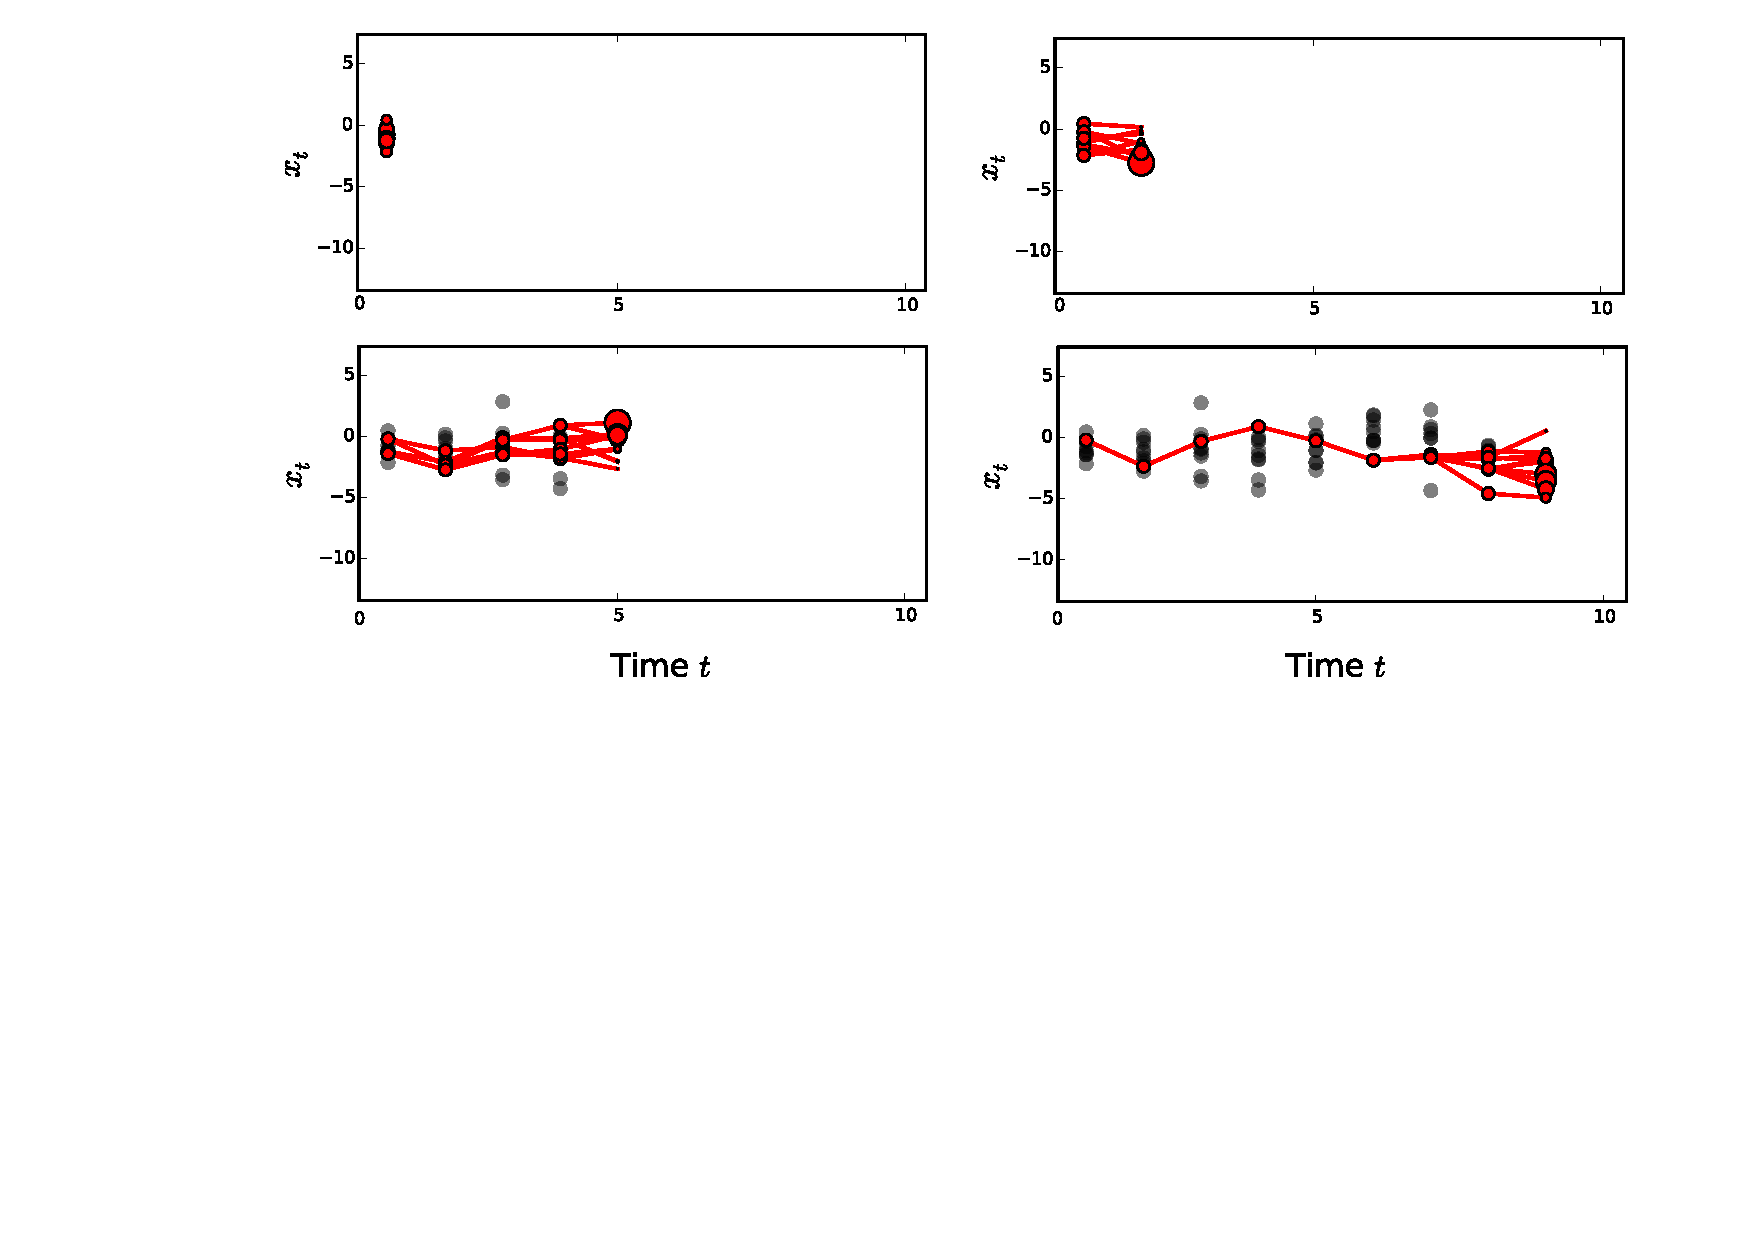
\includegraphics[width=\textwidth]{part/figures/smc_explan}
	\caption{Characterization of the SMC method for a state space model.  At the first time step (top left) 
		we perform importance sampling to approximate $p(x_1 | y_1)$ in the normal way, giving a particle system, or population
		of weighted samples $\{x_1^i,w_1^i\}_{i=1}^N$.  Here each sample is shown by a red blob whose size reflects the weight
		of the particle.  The set of particles are then resampled to produce an unweighted set of particles approximating
		$p(x_1 | y_1)$.  For each of these samples, importance sampling is then used again to produce samples for $x_2$
		by sampling from $q_2 (x_2 | x_1)$ and applying a new importance weight (top right).  Note that, unlike for SIS,
		the importance weights are not propagated from one time step to the next.
		We now again have a weight particle set $\{x_{1:2}^i,w_2^i\}_{i=1}^N$, for which we again perform a resampling
		step to produce an unweighted set of particles.  The process continues in the same way, eventually returning the
		final set of samples $\{x_{1:T}^i,\nw_T^i\}_{i=1}^N$, where we have self-normalized the final weights of each trajectory
		(note that each $\nw_T^i$ applies to the full trajectory $x_{1:T}^i$).  
		Over time, many of the generated samples are
		discarded by the system (shown in gray) during the resampling step.  A consequence of this, which can be seen
		in the bottom right, is that
		many time steps, then our particle set become \emph{degenerate}.  Here we have multiple distinct samples for $x_9$, but
		all our samples share the same \emph{ancestors} for $t=1:6$, i.e. each $x_t^i$ in our final sample set is
		the same for $t\le6$.  We will return to discuss this further in Section~\ref{sec:part:pmcmc:path-deg}.
		\label{fig:part:smc_explan}}
\end{figure}

To see the intuition of why resampling provides the desired resource reallocation, consider what happens 
to the relative weights of different particles in a population if they are propagated through the SIS algorithm at the
same time.  It is easy to see that these weights will quickly diverge, typically exponentially quickly
 (see Section~\ref{sec:inf:foundation:curse}), and our effective sample size 
(see Section~\ref{sec:inf:foundation:ess}) will rapidly diminish.  It is now rather pointless to continue to
propagate the samples with negligible weight through the system as the chance these will have a significant
weight by the end is very low.  We therefore desire a principled way of ``killing off'' these
low weight particles and replacing them with higher weight ones.  As we showed in Section~\ref{sec:inf:foundation:resampling},
resampling gives us a method for generating unweighted samples from a population of weighted samples.
Though resampling itself only duplicates existing particles, rather
than producing new ones, if the duplicate samples are extended independently at the next iteration, this
produces distinct samples (albeit heavily correlated ones).  In other words if we have two samples
$x_{1:t}^1$ and $x_{1:t}^2$ such that $w_t^2/w_t^1 \approx 0$ then it is more beneficial for us to generate both
samples at the next stage using $x_{t+1}^i \sim p(x_{t+1} | x_{1:t}^1, y_{1:t})$ for $i=1,2$, than to use
$x_{1:t}^2$ to sample $x_{t+1}^2$.  This will not improve our representation of $x_{1:t}$, but it will, in
general, give a better representation of the marginal distribution of $x_{t+1}$ and thus the joint distribution
$x_{1:t+1}$.   
%Note that any of the resampling schemes introduced in Section~\ref{sec:inf:foundation:resampling}
%will give rise to valid SMC schemes and so one should, from a practical perspective, generally
%use systematic resampling.

To introduce the \smc method more formally, we consider approximating a sequence of target distributions
in same way as for SIS: in our NMSSM
 case $p(x_{1:t}|y_{1:t}) = p(y_{1:t})^{-1} p(x_{1:t},y_{1:t}), ~t=1,\ldots,T$. 
At each time step $t$ we 
%assume we have access to 
generate a particle system
$\{x_{1:t}^i,w_{t}^i\}_{i=1}^N$ which provides a weighted approximation  to $p(x_{1:t}|y_{1:t})$. Given such a 
weighted particle system, we convert this to an unweighted particle system by resampling as explained
in Section~\ref{sec:inf:foundation:resampling}.  Any of the introduced resampling schemes can be 
used~\citep[Section 4.1]{andrieu2010particle}
and so in general one should use systematic resampling.
When we later introduce PMCMC methods, it will
be useful to think about resampling in terms of propagating particles each particle by drawing an 
ancestor variable $a_{t-1}^i$ (as per~\eqref{eq:inf:resampling}) and then using this to propose the new
variable for that particle, i.e. $x_t^i \sim q_t(x_t | x_{1:t-1}^{a_{t-1}^i})$.  The particle system is then
re-weighted as
\begin{align}
\label{eq:part:smcweights}
w_t^i = \frac{g_t(y_t|x_{1:t}^i) f_t(x_t^i | x_{1:t-1}^{a_{t-1}^i})}{q_t(x_t^i|x_{1:t-1}^{a_{t-1}^i})},
\end{align}
where $x_{1:t}^i = (x_{1:t-1}^{a_{t-1}^i},x_t^i)$.   Note that after resampling,
all the particles have the same weight and therefore, unlike for SIS, the weights at the previous step
do not feature in the weights at the current time step.
This results in a new particle system $\{x_{1:t}^i,w_t^i\}_{i=1}^N$ that approximates $p(x_{1:t}|y_{1:t})$
and the algorithm continues in a self-similar manner up to time $T$.
The overall process is detailed in Algorithm~\ref{alg:part:smc}.  Once run, we can use our final, self-normalized,
particle set $\{x_{1:T}^i,\nw_T^i\}_{i=1}^N$ as a Monte Carlo estimator in the same manner as self-normalized
importance sampling:
\begin{align}
\label{eq:part:smc-est}
\E_{\pi (x_{1:T})} \left[f(x_{1:T})\right] \approx \frac{1}{N} \sum_{i=1}^{N} \nw_T^i f(x_{1:T}^i).
\end{align}

\begin{algorithm}[tb]
	\caption{Sequential Monte Carlo \hfill {\small (all for $i=1,\ldots,N$)}}
	\label{alg:part:smc}
	\begin{spacing}{1.2}
		\begin{algorithmic}[1]
			\renewcommand{\algorithmicrequire}{\textbf{Inputs:}}
			\renewcommand{\algorithmicensure}{\textbf{Outputs:}}				 
			\Require  data $y_{1:T}$, number of particles $N$, proposals $q_t$
			\State $x_1^i \sim q_1(x_1)$
			\State $w_1^i = \frac{g_1(y_1|x_1^i) \mu(x_1^i)}{q_1(x_1^i)}$
			\For{$t = 2$ {\bfseries to} $T$}
			\State $a_{t-1}^i \sim \Discrete\left(\left\{\nw_{t-1}^{\ell}\right\}_{\ell=1}^N\right)$% \tom{We can maybe more general that categorical here?}
			\State $x_t^i \sim q_t(x_t | x_{1:t-1}^{a_{t-1}^i})$ 
			\State Set $x_{1:t}^i = (x_{1:t-1}^{a_{t-1}^i},x_t^i)$
			\State $w_t^i = \frac{g_t(y_t|x_{1:t}^i) f_t(x_t^i | x_{1:t-1}^{a_{t-1}^i})}{q_t(x_t^i|x_{1:t-1}^{a_{t-1}^i})}$
			\EndFor
		\end{algorithmic}
	\end{spacing}
\end{algorithm}

Many intuitions from importance sampling transfer over to SMC.  For example, we can construct our posterior
estimate and calculate expectations in the same way, while we can also use the effective sample size as
a metric of performance (remembering to coalesce identical samples). 
One of the most importance features that translates is that SMC produces the
unbiased estimate for the marginal likelihood $p(y_{1:T})$
\begin{align}
\label{eq:part:ML}
\hat Z = \prod_{t=1}^T \frac{1}{N} \sum_{i=1}^N w_{t}^{i}.
\end{align}
as first shown by~\cite{del2004feynman}.  Although this original
proof requires advanced techniques we will not touch on here, we will later show that this results can also be shown
as a consequence of the proof of correctness for the particle independent Metropolis-Hastings method
given in Section~\ref{sec:part:pmcmc:pimh}.  Note that although the marginal likelihood estimate is
unbiased, the estimator for an general expectation given by~\eqref{eq:part:smc-est} is biased in the same
way as the self-normalized importance sampling estimator given in~\eqref{eq:inf:snis} is.  Nonetheless, producing unbiased
estimates of the marginal likelihood has numerous significant advantages.  

Firstly, it means that one can combine
results from difference SMC runs and still have a consistent estimator for the target and a both unbiased and
consistent estimate for the marginal likelihood.
The is particularly important because the number of particles $N$, is typically restricted by the availability of memory
and we often want to run more than one \emph{SMC sweep} (i.e. single run of SMC).
To combine our estimates, one simply weights each sample by the marginal likelihood of its sweep times
its local, self-normalized, weight $\nw_T^i$, giving the estimator
\begin{align}
\label{eq:part:ind-smc}
\E_{\pi (x_{1:T})} \left[f(x_{1:T})\right] \approx \frac{1}{RN} \sum_{r=1}^{R}\sum_{i=1}^{N} \hat{Z}[r] \nw_T^i[r] f(x_{1:T}^i[r])
\end{align}
where the notation $[r]$ is used to indicates samples from sweep $r$.
 The ability to do this is known as \emph{proper weighting}~\citep{andersson2015nested} and we can justify it by
thinking in terms of using a proposal that first samples a full particle set, giving importance weight $\hat Z$, and then sampling a particle
from this set, giving importance weight $\nw_T^i$.  The product of these separate weights thus gives the weight of
each sample.  

Secondly, the unbiased marginal likelihood estimate means that we can \emph{nest} SMC within other 
methods as a unbiased estimate of the likelihood.
Methods that make use of such unbiased likelihood estimates are known as pseudo-marginal
methods~\citep{andrieu2009pseudo} and will be discussed in Chapter~\ref{chp:nest}.
Some PMCMC methods we introduce in Section~\ref{sec:part:pmcmc} (namely PIMH and PMMH) 
can also be interpreted as pseudo-marginal methods.
%
%The sequential nature of SMC and the resampling step are crucial in making SMC scalable to large $T$.
%The former makes it easier to design efficient proposal distributions as each step need only target 
%the next set of variables $x_t \in \mathcal{X}_t$. 
%The resampling step then allows the algorithm to focus on promising particles in light of new 
%observations, avoiding the exponential divergence between the weights of different samples that 
%occurs for importance sampling as $T$ increases.
%This can be demonstrated both empirically and theoretically \citep[Chapter 9]{del2004feynman}.

\subsection{Sequential Monte Carlo for an Arbitrary Series of Targets}
\label{sec:part:smc:arb}

In its most general form, we can use SMC to target an arbitrary
series of unnormalized target distributions $\left\{\gamma_t (x_{1:t})\right\}_{t=1:T}, \; 
\gamma_t (x_{1:t}) = Z_t \pi_t (x_{1:t})$, each defined on a space
$\mathbb{X}_t$ with strictly increasing dimension\footnote{This restriction
	can be relaxed by using the SMC samplers approach of \citet{del2006sequential}.}
$\mathrm{dim}(\mathbb{X}_{t-1})<\mathrm{dim}(\mathbb{X}_{t})$.
Here $Z_t := \int \gamma_t(x_{1:t}) dx_{1:t}$ is the normalization constant and $\pi_t (x_{1:t})$
the corresponding normalized target.  
The only difference that needs to be made from the NMSSM case is in how the weights
are calculated, with them now given by
\begin{subequations}
\label{eq:part:smc-arb-weights}
\begin{align}
w_1^k &= \frac{\gamma_1(x_1^k)}{q_1(x_1^k)} \\
w_t^k &= \frac{\gamma_t({x}_{1:t}^k)}{\gamma_{t - 1}({x}_{1:t - 1}^{a_{t - 1}^k}) q_t(x_t^i|x_{1:t-1}^{a_{t-1}^i})}.
\end{align}
\end{subequations}
It can be easily seen that the NMSSM weights are a particular case of this, by
plugging in $\gamma_t(x_{1:t}) = p(x_{1:t},y_{1:t})$ into the above expression.  

For inference, then our posterior is the
last target, $\pi_T (x_{1:T})$, with corresponding marginal likelihood $Z_T$.  Using this
more general SMC formulation, we thus see that any series of targets will lead
to a valid inference provided that the final target is the desired posterior and that none
of our intermediate targets place zero probability mass on events that have non-zero
probability mass under the corresponding marginals of the final target 
\begin{align}
\label{eq:part:opt-target}
\tilde{\pi}_t (x_{1:t}) = \int \pi_T (x_{1:T}) dx_{t+1:T}
\end{align}
$\ne \pi_t (x_{1:t})$ in general.  In fact, the series of targets given
for the NMSSM case are actually suboptimal and used because of the fact that
$p(x_{1:t},y_{1:t})$ can, in general, be calculated exactly.  It is a well known result
(see, for example, the appendices of~\cite{le2017auto}) that the optimal series
of proposals (complications with computability and proposals aside) is actually 
the marginals $\tilde{\pi}_t (x_{1:t})=p(x_{1:t} | y_{1:T})$ for
the NMSSM case.  To see this, note that at the $t^{\mathrm{th}}$ step, we are generating 
the samples for $x_{t}$ and so if each of targets is the marginal of the final distribution
$p(x_{1:t} | y_{1:T})$, then the marginal probability of the already sampled variables does not change from
one step to the next.  Conversely, $\pi_t (x_{1:t}) \neq \int \pi_{t+1} (x_{1:t+1}) dx_{t+1}$
in general and so if a different series of targets are used,
e.g. $p(x_{1:t}|y_{1:t})$, then the marginal probability of the already sampled
variables changes from one iteration to the next, reducing the efficient of the inference.
To give an example of this, consider
the case where $x_{1}$ include global parameters that effect each emission
distribution, for example it could contain the variance for Gaussian
likelihood terms.  In our NMSSM case we can never regenerate samples for $x_1$ after
the first step and so it is clearly better at the first step to target $p(x_1 | y_{1:T})$ than $p(x_1|y_1)$,
i.e. to condition on all the data rather than the first datapoint. Unfortunately, calculating
$p(x_1 | y_{1:T})$ itself generally requires a marginalization that is as difficult, or potentially
even more difficult, than the inference itself.  Hence the series of targets we introduced in
the NMSSM formulation are those that are usually used in practice.  However, we note that there are some
innovative methods for partially alleviating this problem, such as block sampling~\citep{doucet2006efficient} methods,
which use a combination of lookahead and \emph{auxiliary weighting} schemes~\citep{cappe2007overview}.
Specifically, they resample using adjusted weights that convey how good the sample is likely
to be a few time steps further down the line.  The bias this would induce is corrected for
by assigning non-even weights to the resampled particles.

Another upshot of the ability to use an arbitrary series of targets is that we can use SMC in scenarios that do not
permit a conventional breakdown of the target distribution, but where we 
can provide guiding distributions to that which we care about.  One possible case is when our prior distribution
is a generative model that can be evaluated on the target dataset at point in generative process.
For example, in~\cite{janz2016probstruct}, we considered the example of doing inference
on the structure of a GP kernel.  Here we can define a generative model that produces
increasingly complex kernels, such that all the intermediary kernels in this generation process are themselves
valid kernels that can thus be evaluated.  Here we can think of expanding our kernel at each time step of 
the SMC inference and our targets as being the posterior on kernel structure for the GP, subject to increasingly
lax restrictions on the kernel complexity.\footnote{Technically in this work actually uses population
	Monte Carlo~\cite{cappe2004population} which is based on using a series of static targets.  The
	intuition, however, predominantly transfers and SMC could have been used instead.}  
Another example is provided by~\cite{lakshminarayanan2013top},
who use SMC for Bayesian learning of decision trees.  Here they use the self-similarity of trees, starting
with a basic stump and then adding a new split at each time step.
For both these problems, SMC has been used
to exploit the fact that the overall problem can be broken down into a series of increasingly difficult
problems, namely those with an increasingly large prior, to guide towards good solutions for the final problem.

\subsection{Practical Considerations}
\label{sec:part:smc:prat}

\subsubsection{Use as Many Particles as Possible}
\label{sec:part:smc:prat:part}

The most important practical consideration for SMC is to
\emph{use as many particles as possible}.  Although, as we showed in~\ref{sec:part:smc:nmssm},
one can run multiple, say $R$, SMC sweeps with $N$ particles each and then combine them using their marginal likelihood estimates, this
is almost exclusively a higher variance (and more skew) estimator than carrying out a single SMC sweep
with $RN$ particles, often many orders of magnitude so.  It is easy to see why a single sweep is preferable
from the point of view of the effect of the different marginal likelihood estimates on the effective sample size.
The reason the number of particles can be so critical is that if it is too small, the variance of the marginal likelihood
estimate explodes, the effective sample size plummets, and one sweep ends up dominating the estimate.  Though the marginal 
likelihood estimate is unbiased, it has a massive positive skew when insufficient particles as used, such that the 
probability that a
sweep gives a marginal likelihood estimate larger than the true marginal likelihood estimate can be arbitrarily small;
after all, the limit $N=1$ corresponds to importance sampling.  As such, if we use insufficient particles and just
repeatedly run SMC sweeps, we may have to wait arbitrarily long before getting any useful samples.  One way 
to try an combat this, presuming it is not possible to increase $N$, is to group the SMC sweeps into a number
of islands and then combined estimates in the normal way within the islands, but combined the islands in
an unweighted fashion (see for example~\cite{lakshminarayanan2013top}).  Though often practically useful, this
is clearly only trading variance for bias and thus is more of a means of mitigating rather than solving the problem.
A more principled means of overcoming this issue is presented by PMCMC methods as discussed in Section~\ref{sec:part:pmcmc}.

\subsubsection{Adaptive Resampling}
\label{sec:part:smc:prat:ad-re}

Another important practical consideration is that it is not always beneficial to resample.  Resampling
obviously throws away information (by reducing the number of distinct particles)
and therefore should not be done spuriously.  As the reason for doing
resampling is to kill off particles with negligible weight, it is generally preferable to avoid the resampling step
when most particles have significant weight.  This lead to the development of so-called \emph{adaptive resampling}
schemes that only perform the resampling step if some criterion is met~\citep{liu1995blind,del2012adaptive}, e.g. 
only resampling when the effective sample size falls below a certain threshold,
for which $N/2$ is a common choice~\cite{doucet2009tutorial}.
When the resampling is omitted, the particles remain unweighted, with their weights at the next iteration updated
using~\eqref{eq:part:sis-weights}, as per SIS, except that the self normalized weights $\bar{w}_t^i$ should be used so that the
marginal likelihood estimate can be carried out in the same manner.
That this still informally forms a valid SMC algorithm for posterior inference can be seen by thinking of these as being sequential importance
sampling steps, noting the equivalence to standard importance sampling, and then viewing the process as simply
skipping some of the intermediate targets, remembering that it is only the final target that we care about.
However, adaptive resampling does cause some complications from a theoretical perspective~\citep{del2012adaptive}.

\subsubsection{Proposals}
\label{sec:part:smc:prat:opt}

The practical performance of SMC can be critically dependent on the choice of proposal and
so we finish our introduction by considering what constitutes a good proposal, first
considering the question of what the theoretically optimal proposal is. Unfortunately it is not generally
possible to establish the optimal proposal for the variance of the final estimate in the finite $N$ case, but we can
calculate the so-called \emph{one-step optimal proposal} by minimizing the variance of the individual weights (and
by proxy the marginal likelihood estimate) at the next iteration.  The one-step optimal proposal is given by
\begin{align}
\label{eq:part:opt-prop}
q_t^*(x_t | x_{1:t-1}) \propto \frac{\gamma_t({x}_{1:t})}{\gamma_{t - 1}({x}_{1:t - 1})} 
\end{align}
$= f_t(x_t | x_{1:t-1}) g_t(y_t | x_{1:t})$ for the NMSSM formulation.  To see why this is optimal we note that
by substituting~\eqref{eq:part:opt-prop} into~\eqref{eq:part:smc-arb-weights} (noting that the proposal needs
to be correctly normalized) then the weights are simply the normalization constant for~\eqref{eq:part:opt-prop}, namely
\begin{align}
w_t(x_{1:t}) &= \int \frac{\gamma_t({x}_{1:t})}{\gamma_{t - 1}({x}_{1:t - 1})} dx_t = 
\frac{\int\gamma_t({x}_{1:t}) dx_t}{\gamma_{t - 1}({x}_{1:t - 1})} 
\end{align}
$=p(y_t | x_{1:t-1})$ for the NMSSM formulation.  Consequently, the weights in the this case are no longer
functions of the sampled value and so the marginal likelihood and effective sample size are deterministic
functions of the particle system before proposing the $x_{t}$, namely of $\{x_{1:t-1}^i,a_{t-1}^i\}_{i=1}^N$.
This also means that we can switch the order of sampling from the proposal and doing the resampling when
using $q_t^*(x_t | x_{1:t-1})$, which is preferable as it increases the diversity in the final sample set.
Note that the weights are not all the same when using the one-step optimal proposal, because
the marginal probability of the particles will change when we incorporate the new observation (or equivalently
move to the new target).  However, given the expected value of each weight is fixed, i.e. $\E [w_t(x_{1:t}) | x_{1:t-1}]=
\frac{\int  \gamma_t({x}_{1:t}) dx_t}{\gamma_{t - 1}({x}_{1:t - 1})} $ regardless of the proposal
used, using any proposal other than the optimal one-step proposal only increases the variance of the estimate
at the next step.  In particular, it is generally
not beneficial to use proposals that include some form of lookahead (e.g. approximating $p(x_{t} |x_{1:t-1},y_{1:T})$
instead of $p(x_{t} |x_{1:t-1},y_{1:t})$), because the resampling step will correct back to the current target and
most likely kill off the ``good'' samples we generated, simply giving us fewer distinct samples than if we had
used the one-step optimal proposal instead.\footnote{Note that lookahead in the proposal is distinct from
	lookahead using auxiliary weights, thus things like block sampling are still useful.}
In both the case where the optimal series of targets~\eqref{eq:part:opt-target} is used and in the large $N$ case, then
the one-step optimal proposal is optimal more generally for the whole SMC sweep for a given series of targets.  However, because it is
not usually possible to analytically calculate the required normalization for $q_t^*(x_t | x_{1:t-1})$, it is
not generally tractable.  Nonetheless, it provides a good guide for designing, or adapting for, effective proposal
distributions.

Another proposal of note, at least for the state space model case, is the so-called bootstrap proposal which
corresponds to sampling from the transition distribution $f_t(x_t | x_{1:t-1})$.  The significance of this proposal
is that it means that the weight calculation given in~\eqref{eq:part:smcweights} cancel to
\begin{align}
\label{eq:part:bootstrap-weights}
w_t^i = g_t (y_t | x_{1:t}^i).
\end{align}
Consequently, if we use the bootstrap proposal we do not need to be able to evaluate the transition distribution
at a particular point, only sample from it.  Obviously this can be helpful for computational reasons (though
it is rare that the effect of this outweighs using a better proposal if one is known), but it is also important
because it can be the case that one only has access to a sampler for the transition and not the ability to evaluate
the transition probability at an arbitrary point.
In the absence of other information, the bootstrap can also be a reasonable choice of proposal in its own right as
it is almost always more diffuse than the one step posterior.  Its efficiency will in general depend on how relatively
peaked the emission distribution is and the dimensionality of $x_t$ -- after all, each step in SMC is in
isolation importance sampling.  One can usually beneficially use the next observation $y_t$ to help guide the
the proposal, but doing this in a general purpose manner can be challenging~\citep{gu2015neural}.
% !TEX root = ../main.tex

\section{Particle Markov Chain Monte Carlo Methods}
\label{sec:part:pmcmc}

Particle Markov chain Monte Carlo (\pmcmc) methods, introduced by \citet{andrieuDH2010}, make use of 
sequential Monte Carlo (\smc) algorithms \citep{gordon1993novel,doucet2001sequential} to construct 
efficient proposals for an \mcmc sampler. This allows it to both utilize the ability of SMC to
exploit the structure of the target problem and the hill climbing behavior of MCMC methods.
The critical difference from running independent SMC sweeps is that information can be transferred
from sweep to the next. 
%The core reason for wanting to do this is that
%one is typically memory restricted in the number of particles that can be run $N$.  Though as we explained
%before, we can run multiple sweeps and combine these using the marginal likelihood estimates, if $N$ is
%not large enough, this typically results it widely varying estimates.  Although these estimates are unbiased,
%they are typically extremely skew, often following a roughly Gaussian distribution in their \emph{log} marginal
%likelihood CITE SOMETHING.  As such, it usually happens if $N$ is not large enough that one sweep dominates the others because
%its marginal likelihood is many orders of magnitude larger than the others and our estimate is
%effectively just the particle sweep with the highest marginal likelihood.  We therefore desire a more principled
%means of transferring the information of one iteration to the next which we can do by constructing an appropriate MCMC
%sampler.  We can then combine the advantages of SMC in its exploitation of the structure of the target with
%the local updating advantages of MCMC methods.  
Naturally this will come with the drawbacks of MCMC samplers
discussed in Section~\ref{sec:inf:foundation:mcmc}, in particular the loss of unbiasedness or marginal likelihood estimates.
However, the advantages will generally outweigh these drawbacks.  PMCMC methods will also allow us to explicitly
treat global parameters of our system differently to the latent states in a manner that can substantially improve
the performance of the model.
Though PMCMC can be applied to models with arbitrary series of targets in the same manner as SMC, we will stick
to the NMSSM case in this section for notational simplicity.

\subsection{Particle Independent Metropolis Hastings}
\label{sec:part:pmcmc:pimh}

Particle independent Metropolis Hastings (PIMH) is the simplest PMCMC algorithm.  Although in isolation it is
not especially useful (as it strictly worse than running independent SMC sweeps and combining 
them),\footnote{There is, though, utility in doing this when also including MCMC steps on global parameters, see~\cite{andrieu2010particle}.}
 it is an
important theoretical stepping stone to more advanced approaches.  The idea from a practical perspective 
is very simple: use an SMC sweep as an independent proposal for an MCMC algorithm targeting $\pi(x_{1:T}) = p(x_{1:T}|y_{1:T})$.
From a theoretical perspective, the approach is rather more profound as it can be viewed as a sampler on 
an \emph{extended space} whose marginal on the returned particles is the target.  
%We will then be able to use
%this to construct more powerful samplers.

\begin{algorithm}[tb]
	\caption{Particle Independent Metropolis Hastings}
	\label{alg:part:pimh}
	\begin{spacing}{1.2}
		\begin{algorithmic}[1]
			\renewcommand{\algorithmicrequire}{\textbf{Inputs:}}
			\renewcommand{\algorithmicensure}{\textbf{Outputs:}}				 
			\Require SMC sampler, number of MCMC iterations R
			\Ensure MCMC samples $\{\hat{x}_{1:T}^r\}_{r=1}^R$
			\State Run SMC giving particle set $X_{1:T}^0 = \{x_{1:T}^{i,0},w_T^{i,0}\}_{i=1}^N$ and marginal likelihood $\hat{Z}^0$
			\State Sample a single particle from set $\hat{x}_{1:T}^0 \sim X_{1:T}^0$ with probability proportional to weight
			\For{$r=2:R$}
			\State Run SMC giving candidate $\tilde{X}_{1:T}^r = \{x_{1:T}^{i,r},w_T^{i,r}\}_{i=1}^N$
				 and $\tilde{Z}^r$
			\If{$u\le \min \left(1,\frac{\tilde{Z}^r}{\hat{Z}^{r-1}}\right)$ where $u\sim \textsc{Uniform}(0,1)$}
			\State $\hat{x}_{1:T}^r \sim \tilde{X}_{1:T}^r, \quad \hat{Z}^{r} \leftarrow \tilde{Z}^r$
			\Else
			\State $\hat{x}_{1:T}^r \leftarrow \hat{x}_{1:T}^{r-1}, \quad \hat{Z}^{r} \leftarrow \hat{Z}^{r-1}$
			\EndIf
			\EndFor
		\end{algorithmic}
	\end{spacing}
\end{algorithm}

The PIMH algorithm is given in Algorithm~\ref{alg:part:pimh}.  We see that PIMH is an MCMC
algorithm where our proposal involves running an independent SMC
sweep and then sampling one of the particles from this particle set in proportion to
the weight of the particle.  This sample is then accepted or rejected using a MH accept-reject
step that  uses the marginal likelihoods of the sweep.  Because our proposal
is independent of our current point, this is strictly worse than just running independent SMC sweeps
(which can also be thought of as applying waste recycling to PIMH ~\citep{frenkel2006waste}).  
It might seem wasteful to only use
one particle from each sweep, but we will be able to Rao-Blackwellize this step and actually
return all the particles at each step as we explain in Section INSERT. 

%Imagine that we were able to exactly calculate the posterior probability of the of samples
%generated by an SMC sweep up to a normalization constant $\gamma(X_{1:T} |y_{1:T})$.  It would
%now be straightforward to construct a valid sampler on this distribution by constructing an independent
%MH proposal and accept/reject the particle sets in the standard way.
The key component of proving the correctness of the PIMH algorithm is in showing that it is a valid
MH sampler on an extended target whose marginal is the distribution of interest.
%The two key components of proving
%the correctness of the PIMH algorithm are in showing that running and SMC sweep then sampling
%one of the samples produced an extended target distribution whose normalized marginal distribution is
%the posterior of interest $\pi(x_{1:T}|y_{1:T})$ and that our MH algorithm remains valid when
%provided with an \emph{unbiased estimate} of the target distribution rather than an exact calculation.
Let $\xib \eqdef \{x_{t}^i\}_{\substack{i=1:N\\t=1:T}} \bigcup \{a_{t}^i\}_{\substack{i=1:N\\t=1:T-1}}$
denote all generated particles and ancestor variables of a \smc sampler.  The density of the distribution induced
by running a SMC sweep is now given by
\begin{align}
\label{eq:part:smc:proposal}
q_{\text{SMC}}(\xib) &= \prod_{i=1}^N q_1(x_{1}^i) \cdot \prod_{t=2}^T \prod_{i=1}^N \left[ 
\nw_{t-1}^{a_{t-1}^i}
%\frac{w_{t-1}^{a_{t-1}^i}}{\sum_\ell w_{t-1}^{\ell}}
q_t(x_{t}^i|x_{1:t-1}^{a_{t-1}^i}) \right]
\end{align}
and the distribution induced by running an SMC sweep and then sampling particle $b$ from the
sample set is 
\begin{align}
q_{\text{PIMH}}(\xib,b) = \bar{w}_T^b q_{\text{SMC}}(\xib) \quad \text{where} \quad \bar{w}_t^i = \frac{{w}_t^i}{\sum_{\ell=1}^{N}w_t^{\ell}}.
\end{align}
Let $\xb^i = x_{1:T,m}^i$ denote one of the final particles and let the trajectory associated
with the particle we sample be $\{\xb^{b},\bb\}$, with $\bb = (\beta_{1,},\ldots,\beta_{T})$,
$\beta_{T} = b$ and $\beta_{t} = a_{t}^{\beta_{t+1}}$. The proof for the validity of the PIMH
algorithm is now demonstrated by showing that it a valid MH sampler for an \emph{extended target distribution}
whose marginal distribution on $\xb^b$ is the distribution of interest $\pi(\xb^b)$.  To construct our
extended target distribution, we consider the following hypothetical sampling process
\begin{enumerate}
	\item Sample a particle exactly from the target $\xb^b \sim \pi(\xb^b)$,
	\item Sample a path for the particle uniformly at random path by independently sampling each $\beta_t \sim \textsc{UniformDiscrete}(1,N)$,
	\item Sample all of the other particles and trajectories conditioned on $\{\xb^{b},\bb\}$ using \begin{align}
	\label{eq:part:csmc}
	q_{\text{CSMC}}\left(\xib \backslash \{\xb', \bb\} \mid \xb', \bb \right) = 
	\prod_{\substack{i=1\\i\neq b_{1}}}^N  q_1(x_{1}^i) \cdot \prod_{t=2}^T \prod_{\substack{i=1\\i\neq b_{t}}}^N \left[
	\nw_{t-1}^{a_{t-1}^i}q_t(x_{t}^i|x_{1:t-1}^{a_{t-1}^i})\right].
	\end{align}
\end{enumerate}
Together these steps induce the distribution
\begin{align}
\label{eq:part:pimh-target}
\tilde{\pi}(\xi,b) = \frac{\pi(\xb^{b})}{N^T} \prod_{i=1, i\neq\beta_1}^N q_1(x_{1}^i) \cdot \prod_{t=2}^T \prod_{i=1, i\neq\beta_t}^N \left[ 
\nw_{t-1}^{a_{t-1}^i}
q_t(x_{t}^i|x_{1:t-1}^{a_{t-1}^i}) \right].
\end{align}
By construction, the marginal of this distribution is $\pi(\xb^{b})$.
Therefore, although it is not possible to actually
sample from $\tilde{\pi}(\xi,b)$ directly (we started the definition by sampling exactly
from the distribution of interest), if we can
construct a consistent MCMC estimator on~\ref{eq:part:pimh-target} then this by proxy
produces a consistent estimator for $\pi(\xb^{b})$.
We can now show that this is exactly what the
PIMH algorithm does by explicitly calculating the importance weight implied by
targeting $\tilde{\pi}(\xi,b)$ using the proposal $q_{\text{PIMH}}(\xib,b)$
\begin{align}
\frac{\tilde{\pi}(\xi,b)}{q_{\text{PIMH}}(\xib,b)} &= \frac{\pi(\xb^{b}) q_{\text{CSMC}}\left(\xib \backslash \{\xb', \bb\} \mid \xb', \bb \right)}
{N^T \bar{w}_T^b q_{\text{SMC}}(\xib)} \\
&= \frac{\pi(\xb^{b})}{N^T \bar{w}_T^b q_1(x_1^{\beta_1}) \prod_{t=2}^{T} \bar{w}_{t-1}^{\beta_{t-1}} q_t(x_t^{\beta_t} | x_{t-1}^{\beta_{t-1}})} \nonumber \\
&= \left(\frac{\gamma(\xb^{b})/Z}{
	q_1(x_1^{\beta_1}) \prod_{t=2}^{T} q_t(x_t^{\beta_t} | x_{t-1}^{\beta_{t-1}})}\right) \cdot
	\left( \frac{1}{N^T \bar{w}_T^b\prod_{t=2}^{T} \bar{w}_{t-1}^{\beta_{t-1}}} \right) \nonumber \\
&= \left(\frac{w_T^b}{Z}
	 \prod_{t=2}^{T} w_{t-1}^{\beta_{t-1}}\right)\cdot\left(
	\frac{1}{N^T \bar{w}_T^b \prod_{t=2}^{T} \bar{w}_{t-1}^{\beta_{t-1}}}\right) \nonumber \\
&= \left(\frac{w_T^b}{Z}
	\prod_{t=2}^{T} w_{t-1}^{\beta_{t-1}}\right)\cdot\left(
	\frac{\prod_{t=1}^T \frac{1}{N} \sum_{\ell=1}^N w_{t}^{\ell}}{w_T^b \prod_{t=2}^{T} w_{t-1}^{\beta_{t-1}}}\right) \nonumber \\
&= \frac{1}{Z} \prod_{t=1}^T \frac{1}{N} \sum_{\ell=1}^N w_{t}^{\ell}
= \frac{\hat{Z}}{Z}.
\end{align}
We thus have that $\hat{Z}$ is the importance weight for sampling the unnormalized
version of the target $\tilde{\gamma}(\xi,b) = Z \tilde{\pi}(\xi,b)$ and so using the
ratio of marginal likelihood estimates provides is exactly the acceptance ratio required for
the MH sampler.  We
have therefore proven that the PIMH algorithm induces a consistent Markov chain for
the target $\pi(x_{1:T})$.

Note that as an aside, this also shows the unbiasedness of the SMC marginal likelihood estimate
as we see that
\begin{align}
\E_{q_{\text{SMC}}(\xib)} \left[\hat{Z}\right] = \E_{q_{\text{PIMH}}(\xib,b)} 
\left[\hat{Z}\right]=\E_{\tilde{\pi}(\xi,b)} \left[Z\right]=Z.
\end{align}
However, SMC will not, in general, provide unbiased estimates for expectations of
functions, for the same reasons that self-normalized importance sampling gives biased
estimates of expectations (see Section~\ref{sec:inf:foundation:importance:self-norm}).

\subsection{Particle Gibbs}
\label{sec:part:pmcmc:pgibbs}

One particularly widely used \pmcmc algorithm is particle Gibbs (\pg). The \pg algorithm modifies the 
\smc step in the \pmcmc algorithm to sample the latent variables conditioned on an existing particle
 trajectory, resulting in what is called a conditional sequential Monte Carlo (\csmc) step. The \pg method
  was first introduced as an efficient Gibbs sampler for latent variable models with static parameters 
  \citep{andrieuDH2010}. Since then, the \pg algorithm and the extension by \citet{lindstenJS2014} have 
  found numerous applications in \eg Bayesian non-parametrics \citep{ValeraFSPC2015,tripuraneni2015}, 
  probabilistic programming \citep{wood2014new,vandemeent_aistats_2015} and graphical models 
  \citep{everitt2012,naessethLS2014,naessethLS2015nested}.  

The \pg algorithm targets the same extended target $\tilde{\pi}(\xib,b)$ as the PIMH algorithm defined
in~\ref{eq:part:pimh-target}, but rather than constructing a MH sampler with independent proposals for
this target, it constructs a Gibbs sampler.  This is done by iteratively 
running \emph{conditional} sequential Monte Carlo (\csmc) sweeps. As described in Algorithm~\ref{alg:csmc},
a \csmc sweep is similar to a standard, unconditional \smc sweep, except that it starts
with an existing \emph{conditional trajectory} $x_{1:T}'$, known as a \emph{retained particle} in the \pg
context, and runs the sweep conditioned on this conditional trajectory being present in the final sample
set.  One can think of this as running a SMC sweep conditioned on the predefined particle surviving each
of the resampling steps.  In other words, the other particles can sample the retained particle as an
ancestor but not vice versa, with the values and ancestral path of the retained particle prefixed. 
 In Algorithm~\ref{alg:csmc} we have
presumed  that this ancestral path is $\bb = (N,\dots,N)$ which is not always the case from a theoretical
perspective.  However, because the path is fixed up front, all possible paths are equivalent from the point
of view of running the sweep.  Therefore,
given we only actually care about the $\xb$ sampled by the algorithm and not the ancestral paths themselves,
we can just use a convenient fixed ancestral path for the retained particle in practice, as done in Algorithm~\ref{alg:csmc}.

\begin{algorithm}[tb]
	\caption{Conditional sequential Monte Carlo}
	\label{alg:csmc}
	\begin{spacing}{1.2}
		\begin{algorithmic}[1]
			\renewcommand{\algorithmicrequire}{\textbf{Inputs:}}
			\renewcommand{\algorithmicensure}{\textbf{Outputs:}}				 
			\Require data $y_{1:T}$, number of particles $N$, proposals $q_t$, conditional trajectory $x_{1:T}'$
			\State $x_1^i \sim q_1(x_1), ~i=1,\ldots,N-1$ and set $x_1^N = x_1'$
			\State $w_1^i = \frac{g_1(y_1|x_1^i) \mu(x_1^i)}{q_1(x_1^i)}, ~i=1,\ldots,N$
			\For{$t = 2$ {\bfseries to} $T$}
			\State $a_{t-1}^i \sim \Discrete\left(\left\{\nw_{t-1}^\ell\right\}_{\ell=1}^N\right), ~i=1,\ldots,N-1$
			\State $x_t^i \sim q_t(x_t | x_{1:t-1}^{a_{t-1}^i}), ~i=1,\ldots,N-1$
			\State Set $a_{t-1}^N = N$ and $x_t^N = x_t'$
			\State Set $x_{1:t}^i = (x_{1:t-1}^{a_{t-1}^i},x_t^i), ~i=1,\ldots,N$
			\State $w_t^i = \frac{g_t(y_t|x_{1:t}^i) f_t(x_t^i | x_{1:t-1}^{a_{t-1}^i})}{q_t(x_t^i|x_{1:t-1}^{a_{t-1}^i})}, ~i=1,\ldots,N$
			\EndFor
		\end{algorithmic}
	\end{spacing}
\end{algorithm}

Unlike \smc sweeps, \csmc sweeps can be linked together by conditioning each sweep using a \emph{retained particle}
sampled from the previous sweep with probability proportional to the final particle weights $\bar{w}^i_T$.
Therefore, once initialized, say using a standard \smc sweep, one can iterate between sampling a retained
particle in the same manner ancestor indices are sampled and running \csmc sweeps conditioned on this
retained particle.  Considerations about global parameters aside (see Section INSERT), this is know
as iterated \csmc and constitutes the \pg algorithm.  A characterization is provided in INSERT. 

\todo[inline]{Add PG characterization figure.}

The theoretical justification for the \pg algorithm can be shown in a similar manner as the PIMH algorithm.
The sampled index $b$ now corresponds the index of the retained particle and we can think of the
approach as alternating between Gibbs updates on $b$ and $\xib \backslash \{\xb,\bb\}$.    In other
words, we alternate between sampling $b \sim \tilde{\pi}(\cdot | \xib)$ and 
$\xib \backslash \{\xb,\bb\} \sim \tilde{\pi}(\cdot | \xb,\bb)$.  \todo[inline]{Continue here}


Though \pg allows for inference over both latent variables and static parameters, 
we will in this paper focus on sampling of the former.  

A drawback of PG is that it can be particularly adversely affected by \emph{path degeneracy} in the CSMC step.  Conditioning on an existing trajectory means that whenever resampling of the trajectories results in a common ancestor, this ancestor must correspond to this trajectory.  Consequently, the mixing of the Markov chain for the early steps in the state sequence can become very slow when the particle set typically coalesces to a single ancestor during the CSMC sweep.
We address this next with the iPMCMC algorithm.

\todo[inline]{Rao-Black}

%In the same way as above for the standard \smc algorithm we can define a joint probability distribution induced by running Algorithm~\ref{alg:csmc} %$q_{\text{CSMC}}(\xb^{1:N},\ab^{1:N}\backslash\{\xb^N,\bb^N\} | \xb^N,\bb^N)$, induced by running Algorithm~\ref{alg:csmc}, where $\xb^N, \bb^N$ is the retained (conditioning) particle. 
%\begin{align}
%&q_{\text{CSMC}}\left(\xb^{1:N},\ab^{1:N} \backslash \{\xb^N, \bb^N\} \mid \xb^N, \bb^N, k \right) = \nonumber \\
%&\prod_{\substack{i=1\\i\neq b_{1}}}^N \left[ q_1(x_{1}^i) \right] \prod_{t=2}^T \prod_{\substack{i=1\\i\neq b_{t}}}^N \left[\frac{W_{t-1}^{a_{t-1}^i}}{\sum_\ell W_{t-1}^\ell} q_t(x_{t}^i|x_{1:t-1}^{a_{t-1}^i})\right],
%\end{align}
%where $\xb^N, \bb^N$ is the retained (conditioning) particle.
%\brooks{doesn't make sense --- if the retained particle is $N$, why is it $\xb_m^k, \bb_m^k$ in the above equation? shouldn't $\xb_m^{1:N},\ab_m^{1:N} \backslash \{\xb_m^k, \bb_m^k\}$ actually be $\xb_m^{1:N-1},\ab_m^{1:N-1}$?}


%
%   Limitations
%
%\subsection{Parallelisation and Limitations}
%\label{sec:limitations}
%Our main goal is to increase the efficiency of particle \mcmc, particle Gibbs especially, by coupling independent \smc methods with \csmc algorithms, perhaps running on different workers or threads. The method we propose, interacting particle Markov chain Monte Carlo (\ipmc), makes efficient use of multi-core and distributed computing architectures to increase accuracy of the Monte Carlo sampler.

%The basic \pg typically suffers from the \emph{path degeneracy} effect of \smc samplers, \ie sample impoverishment due to frequent resampling, which leads to bad mixing of the Markov chain. Since we force one trajectory, the conditional part, to survive to the end it means that for early time steps we will almost always pick the corresponding sample from last iteration. To counteract this we might need a very high number of particles to get good mixing for all latent variables $x_{1:T}$, which can be infeasible due to e.g.~limited available memory. The \ipmc can alleviate this issue by a non-standard coupling of several conditional and unconditional (standard) \smc algorithms. The algorithm lets us, from time to time, completely switch out a \csmc particle system with a completely independent \smc one, resulting in improved mixing of the Markov chain.


% !TEX root = ../../main.tex

\begin{savequote}[8cm]
	An approximate answer to the right problem is worth a good deal more than 
	an exact answer to an approximate problem.
	\qauthor{--- John Tukey}
\end{savequote}


\section{Interacting Particle Markov Chain Monte Carlo}
\label{sec:part:ipmcmc}

In this section we introduce \emph{interacting particle Markov chain Monte Carlo} (\ipmcmc), a \pmcmc method based on an interacting pool of standard and conditional sequential Monte Carlo samplers. Like related methods, \ipmcmc is a Markov chain Monte Carlo sampler on an extended space. We present empirical results that show significant improvements in mixing rates relative to both non-interacting \pmcmc samplers, and a single \pmcmc sampler with an equivalent memory and computational budget. 
An additional advantage of the \ipmcmc method is that it is suitable for distributed and multi-core architectures.  

%!TEX root = ../../main.tex

In this section we introduce \emph{interacting particle Markov chain Monte Carlo} (\ipmcmc)~\citep{rainforth2016interacting}
a \pmcmc method based on an interacting pool of standard and conditional sequential Monte Carlo samplers. Like 
other PMCMC methods, \ipmcmc is a Markov chain Monte Carlo sampler on an extended space. In \ipmcmc we run a pool of 
\csmc and unconditional \smc algorithms as parallel processes that we refer to as nodes. After each run of this pool, 
we apply successive Gibbs updates to the indexes of the \csmc nodes, such that the indices of the \csmc nodes changes. 
Hence, the nodes from which retained particles are sampled can change from one MCMC iteration to the next, reducing
the sensitivity to path degeneracy relative to \pg 
by trading off exploration (\smc) and exploitation (\csmc) to achieve improved mixing of the Markov chains. Crucially, 
the pool provides numerous candidate indices at each Gibbs update, giving a significantly higher probability that an 
entirely new retained particle will be ``switched in'' than in non-interacting alternatives.

We prove that \ipmcmc is a partially collapsed Gibbs sampler on the extended space containing the particle sets for all nodes. 
In the special case where \ipmcmc uses only \emph{one} \csmc node, it can in fact be seen as a non-trivial and unstudied 
instance of the $\alpha$-\smc-based \citep{whiteley2016} \pmcmc method introduced by \citet{huggins2015}. 
However, with \ipmcmc we extend this further to allow for an arbitrary number of \csmc and standard \smc algorithms 
with interaction.

The interaction between nodes requires only minimal communication; each node must report an estimate of the marginal likelihood 
and receive a new role (\smc or \csmc) for the next sweep. This means that \ipmcmc is embarrassingly parallel 
and can be run in a distributed manner on multiple computers.  However, the advantages of \ipmcmc go far beyond
simple parallelization: our experimental evaluation shows that \ipmcmc outperforms both equivalent
non-interacting \pmcmc samplers as well as a single \pg sampler with the same number of particles run longer
to give a matching computational budget.
An implementation of iPMCMC is provided in the probabilistic programming system
\emph{Anglican}\footnote{\angurl} \citep{wood2014new} as we discuss in Chapter~\ref{chp:proginf}.  A general 
purpose toolbox for carrying out iPMCMC and other SMC / PMCMC inference in MATLAB is also provided by the custom
made \emph{probabilistic MATLAB} package.\footnote{\url{https://github.com/twgr/probabilistic_matlab}}
% !TEX root = ../../main.tex

% Here we describe the proposed method and its theoretical properties
\subsection{Method}
\label{sec:method}
%Our main goal with the interacting particle Markov chain Monte Carlo method is to increase the efficiency of particle \mcmc, particle Gibbs especially, by coupling independent \smc methods with \csmc algorithms, perhaps running on different nodes or threads. The method we propose, interacting particle Markov chain Monte Carlo (\ipmc), makes efficient use of multi-core and distributed computing architectures to increase accuracy of the Monte Carlo sampler.

The main goal of \ipmcmc is to increase the efficiency of \pmcmc, in particular \pg. 
As we explain in Section~\ref{sec:part:pmcmc:path-deg}, \pg is especially
susceptible to the \emph{path degeneracy} effect of \smc samplers because the early
time steps in the state-sequence can become stuck in the same position for long
periods if the ancestral paths in the \csmc sweeps typically coalesce to a single sample,
which is by construction guaranteed to be the retained particle.
%The basic \pg algorithm is especially susceptible to the \emph{path degeneracy} effect of \smc samplers, \ie sample impoverishment due to frequent resampling.  Whenever the ancestral lineage collapses at the early stages of the state sequence, the common ancestor is, by construction, guaranteed to be equal to the retained particle.  
This results in high correlation between the samples, and poor mixing of the Markov chain. %Since we force one trajectory, the conditional part, to survive to the end it means that for early time steps we will almost always pick the corresponding sample from last iteration. 
To counteract this we might need a very high number of particles to get good mixing for all latent variables $x_{1:T}$, which can be infeasible due to e.g.~limited available memory. \ipmc can alleviate this issue by, from time to time, switching out a \csmc particle system with a completely independent \smc one, resulting in improved mixing.

\ipmcmc, summarized in Algorithm~\ref{alg:ipmc}, consists of $M$ interacting separate \csmc and \smc algorithms, exchanging only very limited information at each iteration to draw new \mcmc samples. We will refer to these internal \csmc and \smc algorithms as nodes, and assign an index $m=1,\ldots,M$. 
At every iteration, we have $P$ nodes running local \csmc algorithms, with the remaining
$M-P$ nodes running independent \smc.
The \csmc nodes are given an identifier $c_j \in \{1,\ldots,M\}, ~j=1,\ldots,P$ with $c_j \neq c_k,~k \neq j$ and we write $c_{1:P} = \{c_1,\ldots,c_P\}$. Let $\xb_m^i = x_{1:T,m}^i$ be the internal particle trajectories of node $m$.

\begin{algorithm}[tb]
	\caption{\ipmcmc sampler}
	\label{alg:ipmc}
	\begin{spacing}{1.2}
	\begin{algorithmic}[1]
		\renewcommand{\algorithmicrequire}{\textbf{Inputs:}}
		\renewcommand{\algorithmicensure}{\textbf{Outputs:}}				 
		\Require number of nodes $M$, conditional nodes $P$ and \mcmc steps $R$, initial $\xb_{1:P}'[0]$
		\For{$r = 1$ {\bfseries to} $R$}
		\State Workers $1:M \backslash c_{1:P}$ run Algorithm~\ref{alg:part:smc} (\smc)
		\State Workers $c_{1:P}$ run Algorithm~\ref{alg:csmc} (\csmc), conditional on $\xb_{1:P}'[r-1]$ respectively.
		\For{$j = 1$ {\bfseries to} $P$}
		\State Select a new conditional node by simulating $c_j$ according to \eqref{eq:simConditional}. %with probability 
		\State Set new \mcmc sample $\xb_j'[r] = \xb_{c_j}^{b_j}$ by simulating $b_j$ according to~\eqref{eq:simTrajectory}
		\EndFor
		\EndFor
	\end{algorithmic}
\end{spacing}
\end{algorithm}

Suppose we have access to $P$ trajectories ${\xb_{1:P}'[0]=(\xb_1'[0],\ldots,\xb_P'[0])}$ corresponding to the initial retained particles, where the index $[\cdot]$ denotes \mcmc iteration. At each iteration $r$, the nodes $c_{1:P}$ run \csmc (Algorithm~\ref{alg:csmc}) with the previous \mcmc sample $\xb_j'[r-1]$ as the retained particle. The remaining $M-P$ nodes run standard (unconditional) \smc, \ie Algorithm~\ref{alg:part:smc}.  Each node $m$ returns an estimate of the marginal likelihood $\hat Z_{m} $ for the internal particle system
calculated as per~\eqref{eq:part:ML}.  Note that whereas for the \smc sweeps this is an unbiased estimate of the 
marginal likelihood, this a biased estimator for the \csmc sweeps that is being specifically defined for our purposes.
%\begin{align}
%\label{eq:ML}
%\hat Z_{m} = \prod_{t=1}^T \frac{1}{N} \sum_{i=1}^N w_{t,m}^{i}.
%\end{align}
%along with a single trajectory $\xb_{m}^{s_m}$ sampled according to 
%\begin{align}
%\label{eq:simTrajectory}
%\Prb(s_m = i) &= \nw_{T,m}^i
%\end{align}
%where $s_m$ is the local index of the sampled particle.  

The new conditional nodes are then set using a single loop $j=1:P$ of Gibbs updates, sampling new indices $c_j$ where
\begin{align}
\label{eq:simConditional}
&\Prb(c_j = m|c_{1:P\backslash j}) = \hat\nz_{m}^j \\
\label{eq:zeta_def}
\mathrm{and}  \quad &{\hat\nz_{m}^j = \frac{\hat Z_{m} \iden_{m \notin c_{1:P \backslash j}}}{ \sum_{n=1}^M \hat Z_{n} \iden_{n \notin c_{1:P \backslash j}}}},
%\Prb(c_j = m|c_{1:P\backslash j}) = \frac{\hat Z_{\pi,m} \iden_{m \notin c_{1:P \backslash j}}}{\sum_{n=1}^M \hat Z_{\pi,n} \iden_{n \notin c_{1:P \backslash j}}},
\end{align}
defining ${c_{1:P\backslash j} = \{c_1,\ldots,c_{j-1},c_{j+1},\ldots,c_P\}}$.  We thus loop once through the conditional node indices and resample them from the union of the current node index and the unconditional node indices\footnote{Unconditional node indices here refers to all $m \notin c_{1:P}$ at that point in the loop. It may thus include nodes who just ran a CSMC sweep, but have been ``switched out'' earlier in the loop.}, in proportion to their marginal likelihood estimates.  This is the key step that lets us switch completely the nodes from which the retained particles are drawn.


%The retained particles are the corresponding trajectories sampled in \eqref{eq:simTrajectory} such that 
%\begin{align}
%\label{eq:setTrajectory}
%\xb_j'[r] &= \xb_{c_j}^{b_j}, \quad \mathrm{where} \quad b_j = s_{c_j}, \quad j=1,\dots,P.
%\end{align}

%This step, by far the most computationally demanding, can be trivially parallelised over the $M$ nodes. However, it need not be parallelised to see convergence benefits and reduced memory footprints compared to competing \pmcmc methods.
%\begin{figure}[h]
%\centering
%\resizebox{.45\textwidth}{!}{
%\input{./figures/algorithm.tex}
%}
%\caption{A high-level illustration of the \ipmcmc algorithm flow for $M=5$ and $P=2$. \csmc nodes are \emph{red} and \smc nodes are \emph{blue}, which means that for example at iteration $r-1$ we have $c_{1:P} = \{3,5\}$.}\label{fig:algorithm}
%\end{figure}
%\tom{You can't tell the difference between these nodes when printed in black and white so would be good to adjust the colours slightly.  I think the index needs to be m not j?  Also might be nice to have something in caption like here we have have $c_{1:P}[r-1] = {1,2}$ here just allow the figure to be a reference to the notation.} 

%The next step involves exchange of information--we need access to the normalisation constant estimates from each node to sample the next \mcmc output $\xb_j'[r]$. The normalisation constant estimate for each node $m$ is computed using the internal particle system as ${\hat Z_{m} = \prod_{t=1}^T \frac{1}{N} \sum_{i=1}^N w_{t,m}^{i}}$.
%%\begin{align}
%%\hat Z_{\pi,m} = \prod_{t=1}^T \frac{1}{N} \sum_{i=1}^N w_{t,m}^{i}.
%%\end{align}
%%Note that this estimate is unbiased for the standard \smc methods but positively biased for the \csmc{s}. 
%These estimates are then used to set new conditional nodes by simulating new node indices $c_j$ from
%\begin{align}
%\label{eq:simConditional}
%\Prb(c_j = m|c_{1:P\backslash j}) = \hat\nz_{m}^j, \quad j=1,\ldots,P
%%\Prb(c_j = m|c_{1:P\backslash j}) = \frac{\hat Z_{\pi,m} \iden_{m \notin c_{1:P \backslash j}}}{\sum_{n=1}^M \hat Z_{\pi,n} \iden_{n \notin c_{1:P \backslash j}}},
%\end{align}
%with ${\hat\nz_{m}^j = \hat Z_{m} \iden_{m \notin c_{1:P \backslash j}} / \sum_{n=1}^M \hat Z_{n} \iden_{n \notin c_{1:P \backslash j}}}$ and ${c_{1:P\backslash j} = \{c_1,\ldots,c_{j-1},c_{j+1},\ldots,c_P\}}$. This is the key step that lets us switch completely the nodes from which we draw our next \mcmc samples (retained particles) $\xb_{1:P}'[r]$.%This ensures that all the conditional node indices $c_{1:P}$ will be distinct.
%
One \mcmc iteration $r$ is concluded by setting the new samples $\xb_{1:P}'[r]$ by simulating from the corresponding conditional node's, $c_j$, internal particle system in the same way as $b$ was sampled for the \pg algorithm
\begin{align}
\label{eq:simTrajectory}
\Prb(b_j = i | c_j) &= \nw_{T,c_j}^i, \quad %\frac{w_{T,c_j}^{i}}{\sum_\ell w_{T,c_j}^{\ell}}, \nonumber\\
\xb_j'[r] = \xb_{c_j}^{b_j}.
\end{align}
The potential to pick from updated nodes $c_j$, having run independent \smc algorithms, decreases correlation and improves mixing of the  \mcmc sampler. Furthermore, as each Gibbs update corresponds to a one-to-many comparison for maintaining the same conditional index, the probability of switching is much higher than in an analogous non-interacting system.
%A summary of the \ipmcmc algorithm can be found in Algorithm~\ref{alg:ipmc}. % and a high-level overview of the algorithm flow can be found in Figure~\ref{fig:algorithm}.

The theoretical justification for iPMCMC is independent of how the initial trajectories $\xb_{1:P}'[0]$ are generated.  One simple and effective method (that we use in our experiments) is to run standard SMC sweeps for the ``conditional'' nodes at the first iteration.

The \ipmc samples $\xb_{1:P}'[r]$ can be used to estimate expectations for test functions $f: \setX^T \mapsto \reals$ in the standard Monte Carlo sense, with
\begin{align}
\label{eq:mcestimate}
\E[f(\xb)] \approx \frac{1}{RP}\sum_{r=1}^R\sum_{j=1}^P f(\xb_j'[r]).
\end{align}
However, we can improve upon this using Rao-Blackwellization if we have access to all particles generated by the algorithm, 
see Section~\ref{sec:part:ipmcmc:allparticles}.

We note that \ipmcmc is suited to distributed and multi-core architectures. In practise, the particle to be retained, should the node be a conditional node at the next iteration, can be sampled upfront and discarded if unused.  Therefore, at each iteration, only a single particle trajectory and normalisation constant estimate need be communicated between the nodes, whilst the time taken for calculation of the updates of $c_{1:P}$ is negligible.  Further, iPMCMC should be amenable to an asynchronous adaptation under the assumption of a random execution time, independent of $\xb_j'[r-1]$ in Algorithm~\ref{alg:ipmc}. We leave this asynchronous variant to future work.
%\brooks{maybe mention right away that we can improve this?}

%The method we propose is to couple a conditional \smc method with several independent standard \smc{s}. Assume that we have one \csmc and $M-1$ standard \smc processes running, each supplying an estimate of the normalisation constant $p_m^N(y_{1:T}), m=1,\ldots,M$ based on its $N$ particles. 

%The method proceeds by, at each \mcmc iteration, drawing the next process $m^*$ to become the \csmc according to the estimates $\{p_m^N(y_{1:T})\}$. Then, the conditional trajectory $x_{1:t}'$ is drawn from the corresponding process' internal particle representation either by simulating from the final weights or by doing backward simulation \citet{TODO}.

%\begin{algorithm}[tb]
%\caption{Parallel iterated \csmc}
%\label{alg:picsmc}
%\begin{enumerate}
%\item Initialize $x_{1:T}'[0]$ and set $m^* = 1$
%\item \textbf{for $r=1$ to $R$}
%\begin{enumerate}
%\item In process $m \neq m^*$ run $\operatorname{SMC}$
%\item In process $m = m^*$ run $\operatorname{CSMC}(x_{1:T}'[r-1])$
%\item Simulate $m^* \sim \cat \left( \frac{p_m^N(y_{1:T})}{\sum_{\ell=1}^M p_\ell^N(y_{1:T})} \right)$
%\item Extract $x_{1:T}'[r]$ from process $m^*$
%\end{enumerate}
%\end{enumerate}
%\end{algorithm}
%We do this by picking the next conditional trajectory $x_{1:T}'$ in the following way. First, draw a categorical random variable according to


% Theoretical foundation
\subsection{Theoretical Justification}
\label{sec:part:ipmcmc:theory}
In this section we will give some crucial results to justify the proposed \ipmc sampler.
We start by defining some additional notation, much of which is duplicated from the PIMH introduction.
% Let $\nw_t^i \eqdef w_t^i/\sum_\ell w_t^\ell$ denote the normalised importance weights,
% and let 
Let $\xib \eqdef \{x_{t}^i\}_{\substack{i=1:N\\t=1:T}} \bigcup \{a_{t}^i\}_{\substack{i=1:N\\t=1:T-1}}$
denote all generated particles and ancestor variables of a (C)\smc sampler.
We write $\xib_m$ when referring to the variables of the sampler local to node $m$.
%
% We start by denoting the internal particle system, \ie all generated particles and ancestor variables, of node $m$ by $\xib_m \eqdef \{x_{t,m}^i\}_{\substack{i=1:N\\t=1:T}} \bigcup \{a_{t,m}^i\}_{\substack{i=1:N\\t=1:T-1}}$.
Let the conditional particle trajectory and corresponding ancestor variables for node $c_j$ be denoted by $\{\xb_{c_j}^{b_j},\bb_{c_j}\}$, with $\bb_{c_j} = (\beta_{1,c_j},\ldots,\beta_{T,c_j})$,
%\fredrik{I changed to lower case $b_j$ here to agree with (7), but the notation might be a bit confusing. Use a different symbol in (7) or here?}
$\beta_{T,c_j} = b_j$ and $\beta_{t,c_j} = a_{t,c_j}^{\beta_{t+1,c_j}}$. %\tom{Feel that mabye this could do with an extra line of explanation for people not already familiar with this notation from the PMCMC paper}. 
Let the posterior distribution of the latent variables be denoted by $\pi(\xb) \eqdef p(x_{1:T}|y_{1:T})$ with normalisation constant $Z \eqdef p(y_{1:T})$. 
%
Finally we % the induced distributions of the \smc and \csmc algorithms
note that the \smc and \csmc algorithms induce the respective distributions over the random variables
generated by the procedures are given by~\eqref{eq:part:smc:proposal} and~\eqref{eq:part:csmc}
%respectively.
%\vspace{-2mm}
%\begin{align*}
%q_{\text{SMC}}(\xib) &= \prod_{i=1}^N q_1(x_{1}^i) \cdot \prod_{t=2}^T \prod_{i=1}^N \left[ 
%\nw_{t-1}^{a_{t-1}^i}
%%\frac{w_{t-1}^{a_{t-1}^i}}{\sum_\ell w_{t-1}^{\ell}}
%q_t(x_{t}^i|x_{1:t-1}^{a_{t-1}^i}) \right], \\
%q_{\text{CSMC}}\left(\xib \backslash \{\xb', \bb\} \mid \xb', \bb \right) &= \prod_{\substack{i=1\\i\neq b_{1}}}^N  q_1(x_{1}^i) \cdot \prod_{t=2}^T \prod_{\substack{i=1\\i\neq b_{t}}}^N \left[
%\nw_{t-1}^{a_{t-1}^i}
%%\frac{w_{t-1}^{a_{t-1}^i}}{\sum_\ell w_{t-1}^\ell}
%q_t(x_{t}^i|x_{1:t-1}^{a_{t-1}^i})\right].
%\end{align*}
%Note that running Algorithm~\ref{alg:csmc} corresponds to simulating from $q_\text{CSMC}$ using a fixed
%choice for the index variables $\bb = (N\,\ldots,N)$. While these indices are used to facilitate the
%proof of validity of the proposed method, they have no practical relevance and can thus be set to arbitrary
%values, as is done in Algorithm~\ref{alg:csmc}, in a practical implementation.

% \begin{align*}
% &q_{\text{SMC}}(\xib_m) = \nonumber \\
% &\prod_{i=1}^N q_1(x_{1,m}^i) \cdot \prod_{t=2}^T \prod_{i=1}^N \left[ \frac{w_{t-1,m}^{a_{t-1,m}^i}}{\sum_\ell w_{t-1,m}^\ell} q_t(x_{t,m}^i|x_{1:t-1,m}^{a_{t-1,m}^i}) \right],\\
% &q_{\text{CSMC}}\left(\xib_m \backslash \{\xb_m^j, \bb_m\} \mid \xb_m^j, \bb_m, m, j \right) = \nonumber \\
% &\prod_{\substack{i=1\\i\neq b_{1,m}}}^N  q_1(x_{1,m}^i) \cdot \prod_{t=2}^T \prod_{\substack{i=1\\i\neq b_{t,m}}}^N \left[\frac{w_{t-1,m}^{a_{t-1,m}^i}}{\sum_\ell w_{t-1,m}^\ell} q_t(x_{t,m}^i|x_{1:t-1,m}^{a_{t-1,m}^i})\right].
% \end{align*}
Now we are ready to state the main theoretical result.
\begin{theorem}
	\label{thm:one}
	The interacting particle Markov chain Monte Carlo sampler of Algorithm~\ref{alg:ipmc} is a partially collapsed Gibbs sampler \citep{van2008partially} for the target distribution
	\begin{align}
	\label{eq:targetdistribution}
	&\tilde \pi(\xib_{1:M}, c_{1:P}, b_{1:P}) =  \nonumber \\
	&\frac{1}{N^{PT} \binom{M}{P}} \prod_{\substack{m=1\\m\notin c_{1:P}}}^M q_{\text{SMC}}\left(\xib_m\right) \cdot \prod_{j = 1}^P \left[ \pi\left(\xb_{c_j}^{b_j}\right) \iden_{c_j \notin c_{1:j-1}} 
	q_{\text{CSMC}}\left(\xib_{c_j} \backslash \{\xb_{c_j}^{b_j}, \bb_{c_j}\} \mid \xb_{c_j}^{b_j}, \bb_{c_j}\right) \right].
	\end{align}
\end{theorem}
\begin{proof}
	The proof follows similar ideas as our derivation for the PIMH and \pg samplers and thus follows similar ideas
	to those introduced by~\cite{andrieu2010particle}. 
	We prove that the interacting particle Markov chain Monte Carlo sampler is in fact a standard partially collapsed Gibbs sampler \citep{van2008partially} on an extended space \[
	{\Upsilon \eqdef \setX^{\otimes MTN} \times [N]^{\otimes M(T-1)N} \times [M]^{\otimes P} \times [N]^{\otimes P}}.
	\]
	%Assume the setup of Section~\ref{sec:method}. %For convenience, we repeat the target distribution $\tilde\pi(\cdot)$, \ie \eqref{eq:targetdistribution}, on $\Upsilon$ here 
	%\begin{align}
	%\label{app:targetdistribution}
	%&\tilde \pi(\xib_{1:M}, c_{1:P}, b_{1:P}) = \nonumber \\
	%& \frac{1}{N^{PT} \binom{M}{P}} \prod_{\substack{m=1\\m\notin c_{1:P}}}^M q_{\text{SMC}}\left(\xib_m\right) \times \prod_{j = 1}^P \pi\left(\xb_{c_j}^{b_j}\right) \iden_{c_j \notin c_{1:j-1}} \nonumber \\
	%&\prod_{j = 1}^P q_{\text{CSMC}}\left(\xib_{c_j} \backslash \{\xb_{c_j}^{b_j}, \bb_{c_j}\} \mid \xb_{c_j}^{b_j}, \bb_{c_j}, c_j, b_j \right).
	%\end{align}
	%\begin{align}
	%\label{eq:supptargetdist}
	%\tilde \pi(\xb_{1:M}^{1:N}, \ab_{1:M}^{1:N}, C_{1:P}, B_{1:P}) &= \frac{1}{N^{PT} \binom{M}{P}} \prod_{\substack{m=1\\m\notin C_{1:P}}}^M q_{\text{SMC}}\left(\xb_m^{1:N},\ab_m^{1:N}\right)  \times \prod_{j = 1}^P \pi\left(\xb_{C_j}^{B_j}\right) \mathbbm{1}_{C_j \notin C_{1:j-1}}  \nonumber\\
	%&\times \prod_{j = 1}^P q_{\text{CSMC}}\left(\xb_{C_j}^{1:N},\ab_{C_j}^{1:N} \backslash \{\xb_{C_j}^{B_j}, \bb_{C_j}^{B_j}\} \mid \xb_{C_j}^{B_j}, \bb_{C_j}^{B_j}, C_j, B_j \right),
	%\end{align}
	%with $q_{\text{SMC}}(\cdot), ~q_{\text{CSMC}}(\cdot)$ given by the following expressions
	%\begin{align}
	%q_{\text{SMC}}(\xb_m^{1:N},\ab_m^{1:N}) &= \prod_{i=1}^N q_1(x_1^i) \prod_{t=2}^T \frac{W_{t-1}^{a_{t-1,m}^i}}{\sum_\ell W_{t-1,m}^\ell} q_t(x_{t,m}^i|x_{1:t-1,m}^{a_{t-1,m}^i}),\\
	%q_{\text{CSMC}}\left(\xb_m^{1:N},\ab_m^{1:N} \backslash \{\xb_m^k, \bb_m^k\} \mid \xb_m^k, \bb_m^k, m, k \right) &= \prod_{\substack{i=1\\i\neq b_{1,m}}}^N q_1(x_{1,m}^i) \prod_{t=2}^T \prod_{\substack{i=1\\i\neq b_{t,m}}}^N\frac{W_{t-1,m}^{a_{t-1,m}^i}}{\sum_\ell W_{t-1,m}^\ell} q_t(x_{t,m}^i|x_{1:t-1,m}^{a_{t-1,m}^i}),
	%\end{align}
	%where $\bb_m^k = (b_{1,m},\ldots,b_{T,m})$ with the conditional trajectory indices defined recursively as follows $b_{T,m} = k$ and $b_{t,m} = a_{t,m}^{b_{t+1,m}}$.
	With $\tilde\pi(\cdot)$ with as per \eqref{eq:targetdistribution}, we will show that following the Gibbs sampler on $\Upsilon$
	\begin{subequations}
		\label{eq:gibbs}
		\begin{align}
		\xib_{1:M} \backslash\{\xb_{c_{1:P}}^{b_{1:P}}, \bb_{c_{1:P}} \} ~&\sim \tilde \pi(~\cdot~|\xb_{c_{1:P}}^{b_{1:P}}, \bb_{c_{1:P}},c_{1:P}, b_{1:P})\label{eq:particles},\\
		c_j &\sim \tilde \pi(~\cdot~|\xib_{1:M}, c_{1:P\backslash j}), ~~j=1,\ldots,P,\label{eq:worker}\\
		b_j &\sim \tilde \pi(~\cdot~|\xib_{1:M}, c_{1:P}), ~~j=1,\ldots,P,\label{eq:index}
		\end{align}
	\end{subequations}
	is equivalent to the \ipmcmc method laid out in Algorithm~\ref{alg:ipmc}.
	%where $\tilde \pi( \cdot )$ is given by \eqref{eq:supptargetdist}.
	
	First, the initial step \eqref{eq:particles} corresponds to sampling from
	\begin{align*}
	\tilde\pi(\xib_{1:M} &\backslash\{\xb_{c_{1:P}}^{b_{1:P}}, \bb_{c_{1:P}} \} | \xb_{c_{1:P}}^{b_{1:P}}, \bb_{c_{1:P}},c_{1:P}, b_{1:P}) = \\ 
	& \prod_{m=1,m\notin c_{1:P}}^M q_{\text{SMC}}\left(\xib_m\right) \prod_{j = 1}^P q_{\text{CSMC}}\left(\xib_{c_j} \backslash \{\xb_{c_j}^{b_j}, \bb_{c_j}\} \mid \xb_{c_j}^{b_j}, \bb_{c_j}, c_j, b_j \right).
	\end{align*}
	Given the conditional trajectories, this just corresponds to steps 3--4 in Algorithm~\ref{alg:ipmc}, 
	\ie running $P$ \csmc and $M-P$ \smc algorithms independently.
	We continue with a reformulation of \eqref{eq:targetdistribution} which will be useful to prove correctness for the other two steps.
	Here we first note that
	\begin{align}
	\tilde \pi (\xib_{1:M},  c_{1:P}, & b_{1:P})=\frac{1}{\binom{M}{P}} \prod_{m=1}^M q_{\text{SMC}}\left(\xib_m\right) \nonumber\\ &\cdot
	\prod_{j = 1}^P \left[
	\iden_{c_j \notin c_{1:j-1}} \nw_{T,c_j}^{b_j}
	\frac{\pi\left(\xb_{c_j}^{b_j}\right) q_{\text{CSMC}}\left(\xib_{c_j} \backslash \{\xb_{c_j}^{b_j}, \bb_{c_j}\} \mid 
		\xb_{c_j}^{b_j}, \bb_{c_j}, c_j, b_j \right)}{N^{T} \nw_{T,c_j}^{b_j}q_{\text{SMC}}\left(\xib_{c_j}\right)}\right].
	\end{align}
	Now by self similarity to importance weight calculated for the PIMH derivation in~\eqref{eq:part:pimh-w}
	\begin{align}
	\frac{\pi\left(\xb_{c_j}^{b_j}\right) q_{\text{CSMC}}\left(\xib_{c_j} \backslash \{\xb_{c_j}^{b_j}, \bb_{c_j}\} \mid 
		\xb_{c_j}^{b_j}, \bb_{c_j}, c_j, b_j \right)}{N^{T} \nw_{T,c_j}^{b_j}q_{\text{SMC}}\left(\xib_{c_j}\right)}
	= \frac{\hat Z_{c_j}}{Z}
	\end{align}
	and therefore
	\begin{align}
		\label{eq:reformtargetdist}
	\tilde \pi (\xib_{1:M},  c_{1:P}, b_{1:P}) &= \frac{1}{\binom{M}{P}} \prod_{m=1}^M q_{\text{SMC}}\left(\xib_m\right) \cdot \prod_{j = 1}^P \frac{\hat Z_{c_j}}{Z}\iden_{c_j \notin c_{1:j-1}} 
	\nw_{T,c_j}^{b_j}.
	\end{align}
	By marginalizing this reformulation over $b_{1:P}$ we get
	\begin{align*}
	\tilde\pi(\xib_{1:M}, c_{1:P}) 
	%&= \sum_{b_{1:P}}\tilde\pi(\xib_{1:M}, c_{1:P}, b_{1:P}) \nonumber \\
	&= \frac{1}{\binom{M}{P}} \prod_{m=1}^M q_{\text{SMC}}\left(\xib_m\right) \prod_{j = 1}^P \frac{\hat Z_{c_j}}{Z}\iden_{c_j \notin c_{1:j-1}} .\nonumber
	\end{align*}
	From this it is easy to see that $\tilde\pi(c_j | \xib_{1:M}, c_{1:P\backslash j}) = \hat\nz_{c_j}^j$, which 
	%\begin{align*}
	%\tilde\pi(c_j | \xib_{1:M}, c_{1:P\backslash j}) = \hat\nz_{\pi,c_j}^j
	%\tilde\pi(c_j | \xib_{1:M}, c_{1:P\backslash j}) = \frac{\hat Z_{\pi,c_j} \iden_{c_j \notin c_{1:P\backslash j}}}{\sum_{m=1}^M \hat Z_{\pi,m} \iden_{m \notin c_{1:P\backslash j}}}
	%\end{align*}
	corresponds to sampling the conditional node indices, \ie step 6 in Algorithm~\ref{alg:ipmc}. Finally, from \eqref{eq:reformtargetdist} we can see that simulating $b_{1:P}$ can be done independently as follows
	\begin{align*}
	&\tilde\pi(b_{1:P} | \xib_{1:M}, c_{1:P}) = \frac{\tilde\pi(b_{1:P} ,\xib_{1:M}, c_{1:P})}{\tilde\pi(\xib_{1:M}, c_{1:P})} =  \prod_{j = 1}^P 
	\nw_{T,c_j}^{b_j}
	%\frac{w_{T,c_j}^{b_j}}{\sum_{i=1}^N w_{T,c_j}^i}
	.
	\end{align*}
	This corresponds to step 7 in Algorithm~\ref{alg:ipmc}. We now have that the procedure defined 
	by \eqref{eq:gibbs} is a partially collapsed Gibbs sampler, derived from \eqref{eq:targetdistribution}, 
	and we have shown that it is exactly equal to the \ipmcmc sampler described in Algorithm~\ref{alg:ipmc}.
	\vspace{-8pt}
\end{proof}
\newtheorem{rem}{Remark}
\begin{rem}
	The marginal distribution of $(\xb_{c_{1:P}}^{b_{1:P}},c_{1:P},b_{1:P})$, with $\xb_{c_{1:P}}^{b_{1:P}} = (\xb_{c_1}^{b_1},\ldots,\xb_{c_P}^{b_P})$, under \eqref{eq:targetdistribution} is by construction given by
	\vspace{-4pt}
	\begin{align}
	\label{eq:marginaldistribution}
	&\tilde \pi\left(\xb_{c_{1:P}}^{b_{1:P}},c_{1:P},b_{1:P}\right) = \frac{\prod_{j = 1}^P \pi\left(\xb_{c_j}^{b_j}\right) \iden_{c_j \notin c_{1:j-1}}}{N^{PT} \binom{M}{P}}
	\end{align}
	because our extended target is formulated as being the process of sampling exactly from~\eqref{eq:marginaldistribution}
	and then running the $P$ \csmc sweeps and $M-P$ \smc sweeps.
	This means that each trajectory $\xb_{c_j}^{b_j}$ is marginally distributed according to the
	posterior distribution of interest, $\pi$. Indeed, the $P$ retained trajectories of \ipmcmc
	will in the limit $R \rightarrow \infty$ %(or $N \rightarrow \infty$) 
	be independent draws from $\pi$.  Note similarly that it follows that~\eqref{eq:mcestimate}
	is a consistent estimator (as $R\rightarrow\infty$).
	% , by targeting \eqref{eq:targetdistribution} with an \mcmc sampler we will, in the limit, equivivalently draw $P$ exact samples from $\pi$ as a byproduct at each iteration.
	\vspace{-8pt}
\end{rem}
\noindent Note that adding a backward or ancestor simulation step can drastically increase mixing when sampling the conditional trajectories $\xb_j'[r]$ \citep{lindsten2013backward}. In the \ipmcmc sampler we can replace simulating from the final weights on line~7 by a backward simulation step. Another option for the \csmc nodes is to replace this step by internal ancestor sampling \citep{lindstenJS2014} steps and simulate from the final weights as normal.
%According to the above remark if we can generate samples from \eqref{eq:targetdistribution} we will equivivalently draw exact samples from $\pi$ as a byproduct. We formalize this and show a basic convergence result of the \mcmc samples $\xb^{1:P}[r]$ generated by running Algorithm~\ref{alg:ipmc}.
%\begin{theorem}[Convergence]
%\begin{align}
%\label{eq:convergence}
%\|\mathcal{L}\{\xb^j[r] \in \cdot \}-\pi(\cdot) \| \rightarrow 0, \quad \text{as}~~r\to\infty,~\forall j=1,\ldots,P
%\end{align}
%\end{theorem}
%\begin{proof}
%See Section~\ref{} in the supplementary material.
%\end{proof}

% Parameters, Rao-Blackwellization, BS etc.
%\subsection{Extensions and Improvements}
%We will here discuss some potential extensions and improvements on the \ipmcmc. The first one, making use of all particles, we use in the experiments and the following two, introducing backward simulation and asynchronous implementation, we leave for future work.


% How to use all particles when estimating expectations
\subsection{Using All the Particles}
\label{sec:part:ipmcmc:allparticles}
\vspace{-4pt}
As we discussed for the PIMH and \pg cases in Section~\ref{sec:part:pmcmc:all},
it can be wasteful to throw away most of our generated samples.  Thankfully we
can again carry out a Rao-Blackwellization for \ipmcmc to 
make use of all particles when estimating expectations of interest.  To do this
we will at each Gibbs update $j$, averaging over the possible new values for the 
conditional node index $c_j$ and corresponding particle index $b_j$. We can do this by replacing $\frac{1}{P}\sum_{j=1}^P f(\xb_j'[r])$ 
in \eqref{eq:mcestimate} by
\begin{align*}
\frac{1}{P}\sum_{j=1}^P \E\left[f(\xb_j'[r]) \middle| \xi_{1:M}, c_{1:P\backslash j} \right] 
=\frac{1}{P} \sum_{m=1}^M  \left[\left(\sum_{j=1}^P \hat \zeta_m^j \right) \cdot 
\left(\sum_{i=1}^N \bar w_{T,m}^i  f(\xb_{m}^{i}) \right)\right]
%= \sum_{m=1}^M 
%\hat\nz_{m}^j
%%\frac{\hat Z_{\pi,m} \iden_{m \notin c_{1:P \backslash j}}}{\sum_n \hat Z_{\pi,n} \iden_{n \notin c_{1:P \backslash j}}} 
%\sum_{i=1}^N
%\nw_{T,m}^i f(\xb_{m}^i),
%\frac{w_{T,m}^{i}}{\sum_\ell w_{T,m}^{\ell}} f(\xb_{m}^i),
\end{align*}
where the expectation is over $b_j$ and $c_j$.
We highlight that each $\hat\nz_{m}^j$, as defined in~\eqref{eq:zeta_def}, 
depends on which indices are sampled earlier in the index reassignment loop.  

To derive this we first note that for iteration $r$ we calculate
$\frac{1}{P}\sum_{j=1}^P f(\xb_j'[r]) = \frac{1}{P}\sum_{j=1}^P f(\xb_{c_j}^{b_j})$
where we can Rao-Blackwellize the selection of the retained particle along with each individual Gibbs update
and thereby replace $f(\xb_{c_j}^{b_j})$ with its expectation over $c_j$ and $b_j$
as follows
\begin{align*}
\frac{1}{P} & \sum_{j=1}^P \E \left[f(\xb_{c_j}^{b_j}) \middle| \xi_{1:M}, c_{1:P\backslash j} \right] =
\frac{1}{P}\sum_{j=1}^P \E \left[\sum_{i=1}^N \bar w_{T,c_j}^i  f(\xb_{c_j}^{i}) \middle| \xi_{1:M}, c_{1:P\backslash j} \right] \\ 
%=& \frac{1}{P}\sum_{j=1}^P \sum_{i=1}^N \E \left[\bar w_{T,c_j}^i  f(\xb_{c_j}^{i}) \middle| \xi_{1:M}, c_{1:P\backslash j}  \right] \\
&\quad \quad = \frac{1}{P}\sum_{j=1}^P \sum_{i=1}^N \sum_{m=1}^M \hat \zeta_m^j \bar w_{T,m}^i  f(\xb_{m}^{i})
%=& \frac{1}{P}\sum_{j=1}^P \sum_{m=1}^M \hat \zeta_m^j \sum_{i=1}^N \bar w_{T,m}^i  f(\xb_{m}^{i})\\
= \frac{1}{P} \sum_{m=1}^M  \left[\left(\sum_{j=1}^P \hat \zeta_m^j \right) \cdot \left(\sum_{i=1}^N \bar w_{T,m}^i  f(\xb_{m}^{i}) \right)\right].
%&\E_{c_j|c_{1:P\backslash j}}\left[\E_{b_{1:P}}\left[\frac{1}{P}\sum_{j=1}^P f(\xb_{c_j}^{b_j})\right]\right] = \frac{1}{P}\sum_{j=1}^P \E_{c_j|c_{1:P\backslash j}}\left[\E_{b_{1:P}}\left[ f(\xb_{c_j}^{b_j})\right]\right] = \frac{1}{P}\sum_{j=1}^P \E_{c_j|c_{1:P\backslash j}}\left[ \sum_{i=1}^N \bar w_{T,c_j}^i  f(\xb_{c_j}^{i})\right] \\
%&= \frac{1}{P}\sum_{j=1}^P \sum_{i=1}^N \E_{c_j|c_{1:P\backslash j}}\left[ \bar w_{T,c_j}^i  f(\xb_{c_j}^{i})\right] = \frac{1}{P}\sum_{j=1}^P \sum_{i=1}^N \sum_{m=1}^M \hat \zeta_m^j \bar w_{T,m}^i  f(\xb_{m}^{i}) = \frac{1}{P}\sum_{j=1}^P \sum_{m=1}^M \hat \zeta_m^j \sum_{i=1}^N \bar w_{T,m}^i  f(\xb_{m}^{i}),
\end{align*}
Here we have made use of the knowledge that the internal particle system $\{(\xb_{m}^{i},\bar w_{T,m}^i)\}$ does not change between Gibbs updates of the $c_j$'s, whereas the $\hat \zeta_m^j$ do.  We emphasise that this is a separate Rao-Blackwellization of each Gibbs update of the conditional node indices, such that each is conditioned upon the actual update made at $j-1$, rather than a simultaneous Rao-Blackwellization of the full batch of $P$ updates.  Though the latter also has analytic form and should theoretically be lower variance, it suffers from inherent numerical instability and so is difficult to calculate in practise.  We found that empirically there was not a noticeable difference between the performance of the two procedures.  Furthermore, one can always run additional Gibbs updates on the $c_j$'s and obtain an improve estimate on the relative sample weightings if desired.

%\tom{I feel it might be better to move the asynchronous and backward simulation to the discussion section given we are leaving them for future work?}

% Introduce \theta and sample that as well
%\subsubsection{Static Parameters}
%We can also use the \ipmcmc algorithm to sample static parameters $\theta$ in a Gibbs-type method by alternating between sampling latent variables $x_{1:T}$ and $\theta$. The basic version of this would add two extra steps in Algorithm~\ref{alg:ipmc} by simulating new parameters from the full conditional distributions for the \csmc nodes and the parameter prior for the standard \smc nodes.

\subsection{Choosing P}
\label{sec:part:ipmcmc:choosingP}
Before jumping into the full details of our experimentation, we quickly consider the choice of $P$. Intuitively we can think of the independent \smc's as particularly useful if they are selected as the next conditional node. The probability of the event %(denoted by $\mathcal{S}$) 
that at least one conditional node switches with an unconditional, is given by
\begin{align}
\label{eq:switchingprob}
%\Prb(\mathcal{S}) 
\Prb(\{\text{switch}\}) 
= 1 - \E\Big[\prod_{j=1}^P \frac{\hat Z_{c_j}}{\hat Z_{c_j} +\sum_{m \notin c_{1:P}}^M \hat Z_{m}}\Big].
\end{align}
There exist theoretical and experimental results \citep{pitt2012some,berard2014lognormal,doucet2015efficient} that show that the distributions of the normalisation constants are well-approximated by their log-Normal limiting distributions. With $\sigma^2$ ($\propto \frac{1}{N}$) being the variance of the (C)\smc estimate, we have $\log \left(Z^{-1} \hat Z_{c_j} \right) \sim \N(\frac{\sigma^2}{2},\sigma^2)$ and $\log \left(Z^{-1} \hat Z_{m} \right) \sim \N(-\frac{\sigma^2}{2},\sigma^2)$, $m\notin c_{1:P}$ at stationarity, where $Z$ is the true normalization constant. Under this assumption, we can accurately estimate the probability \eqref{eq:switchingprob} for different choices of $P$ an example of which is shown in Figure~\ref{fig:theSwitchingProb} along with additional analysis given in the supplementary material of~\cite{rainforth2016interacting}. These provide strong empirical evidence that the switching probability is maximised for $P=M/2$.

\begin{figure}[t]
	\centering
	\begin{subfigure}[t]{0.4\textwidth}
		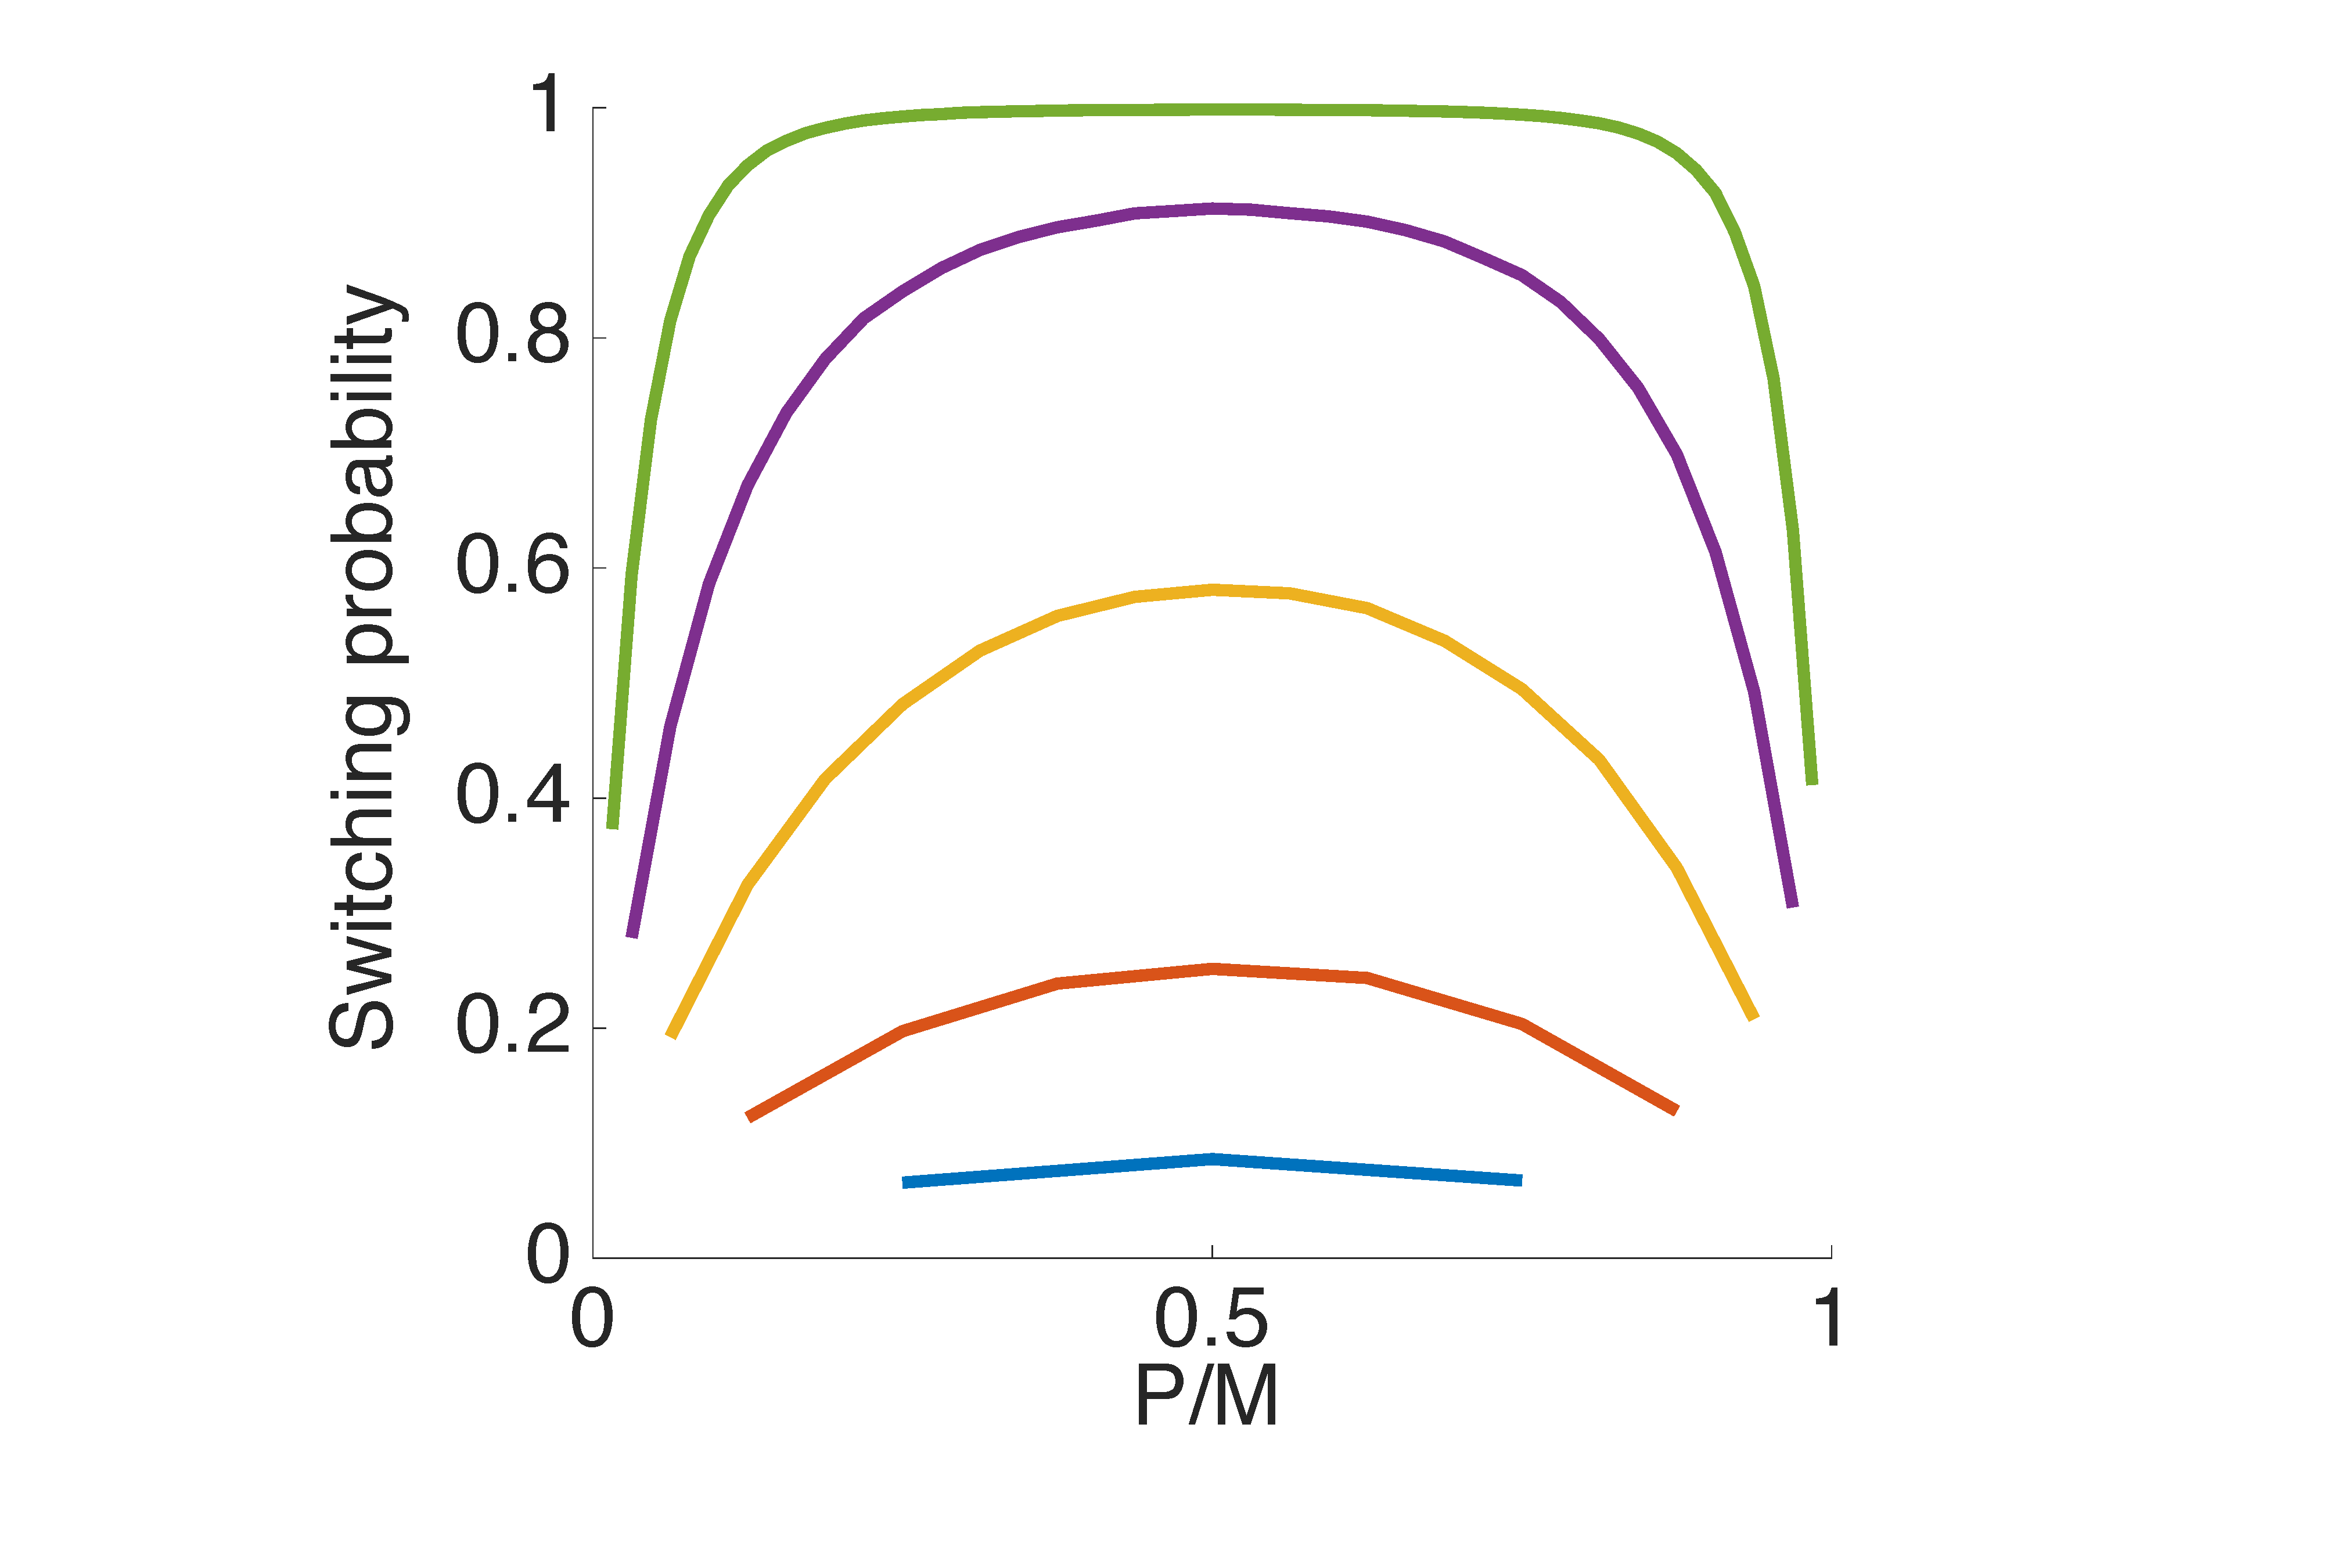
\includegraphics[height=0.75\textwidth]{swtiching_prob_sweep_sigma_3}
		\caption{Limiting log-Normal\label{fig:theSwitchingProb}}
	\end{subfigure}
	~~~~~~~~~~~
	\begin{subfigure}[t]{0.4\textwidth}
		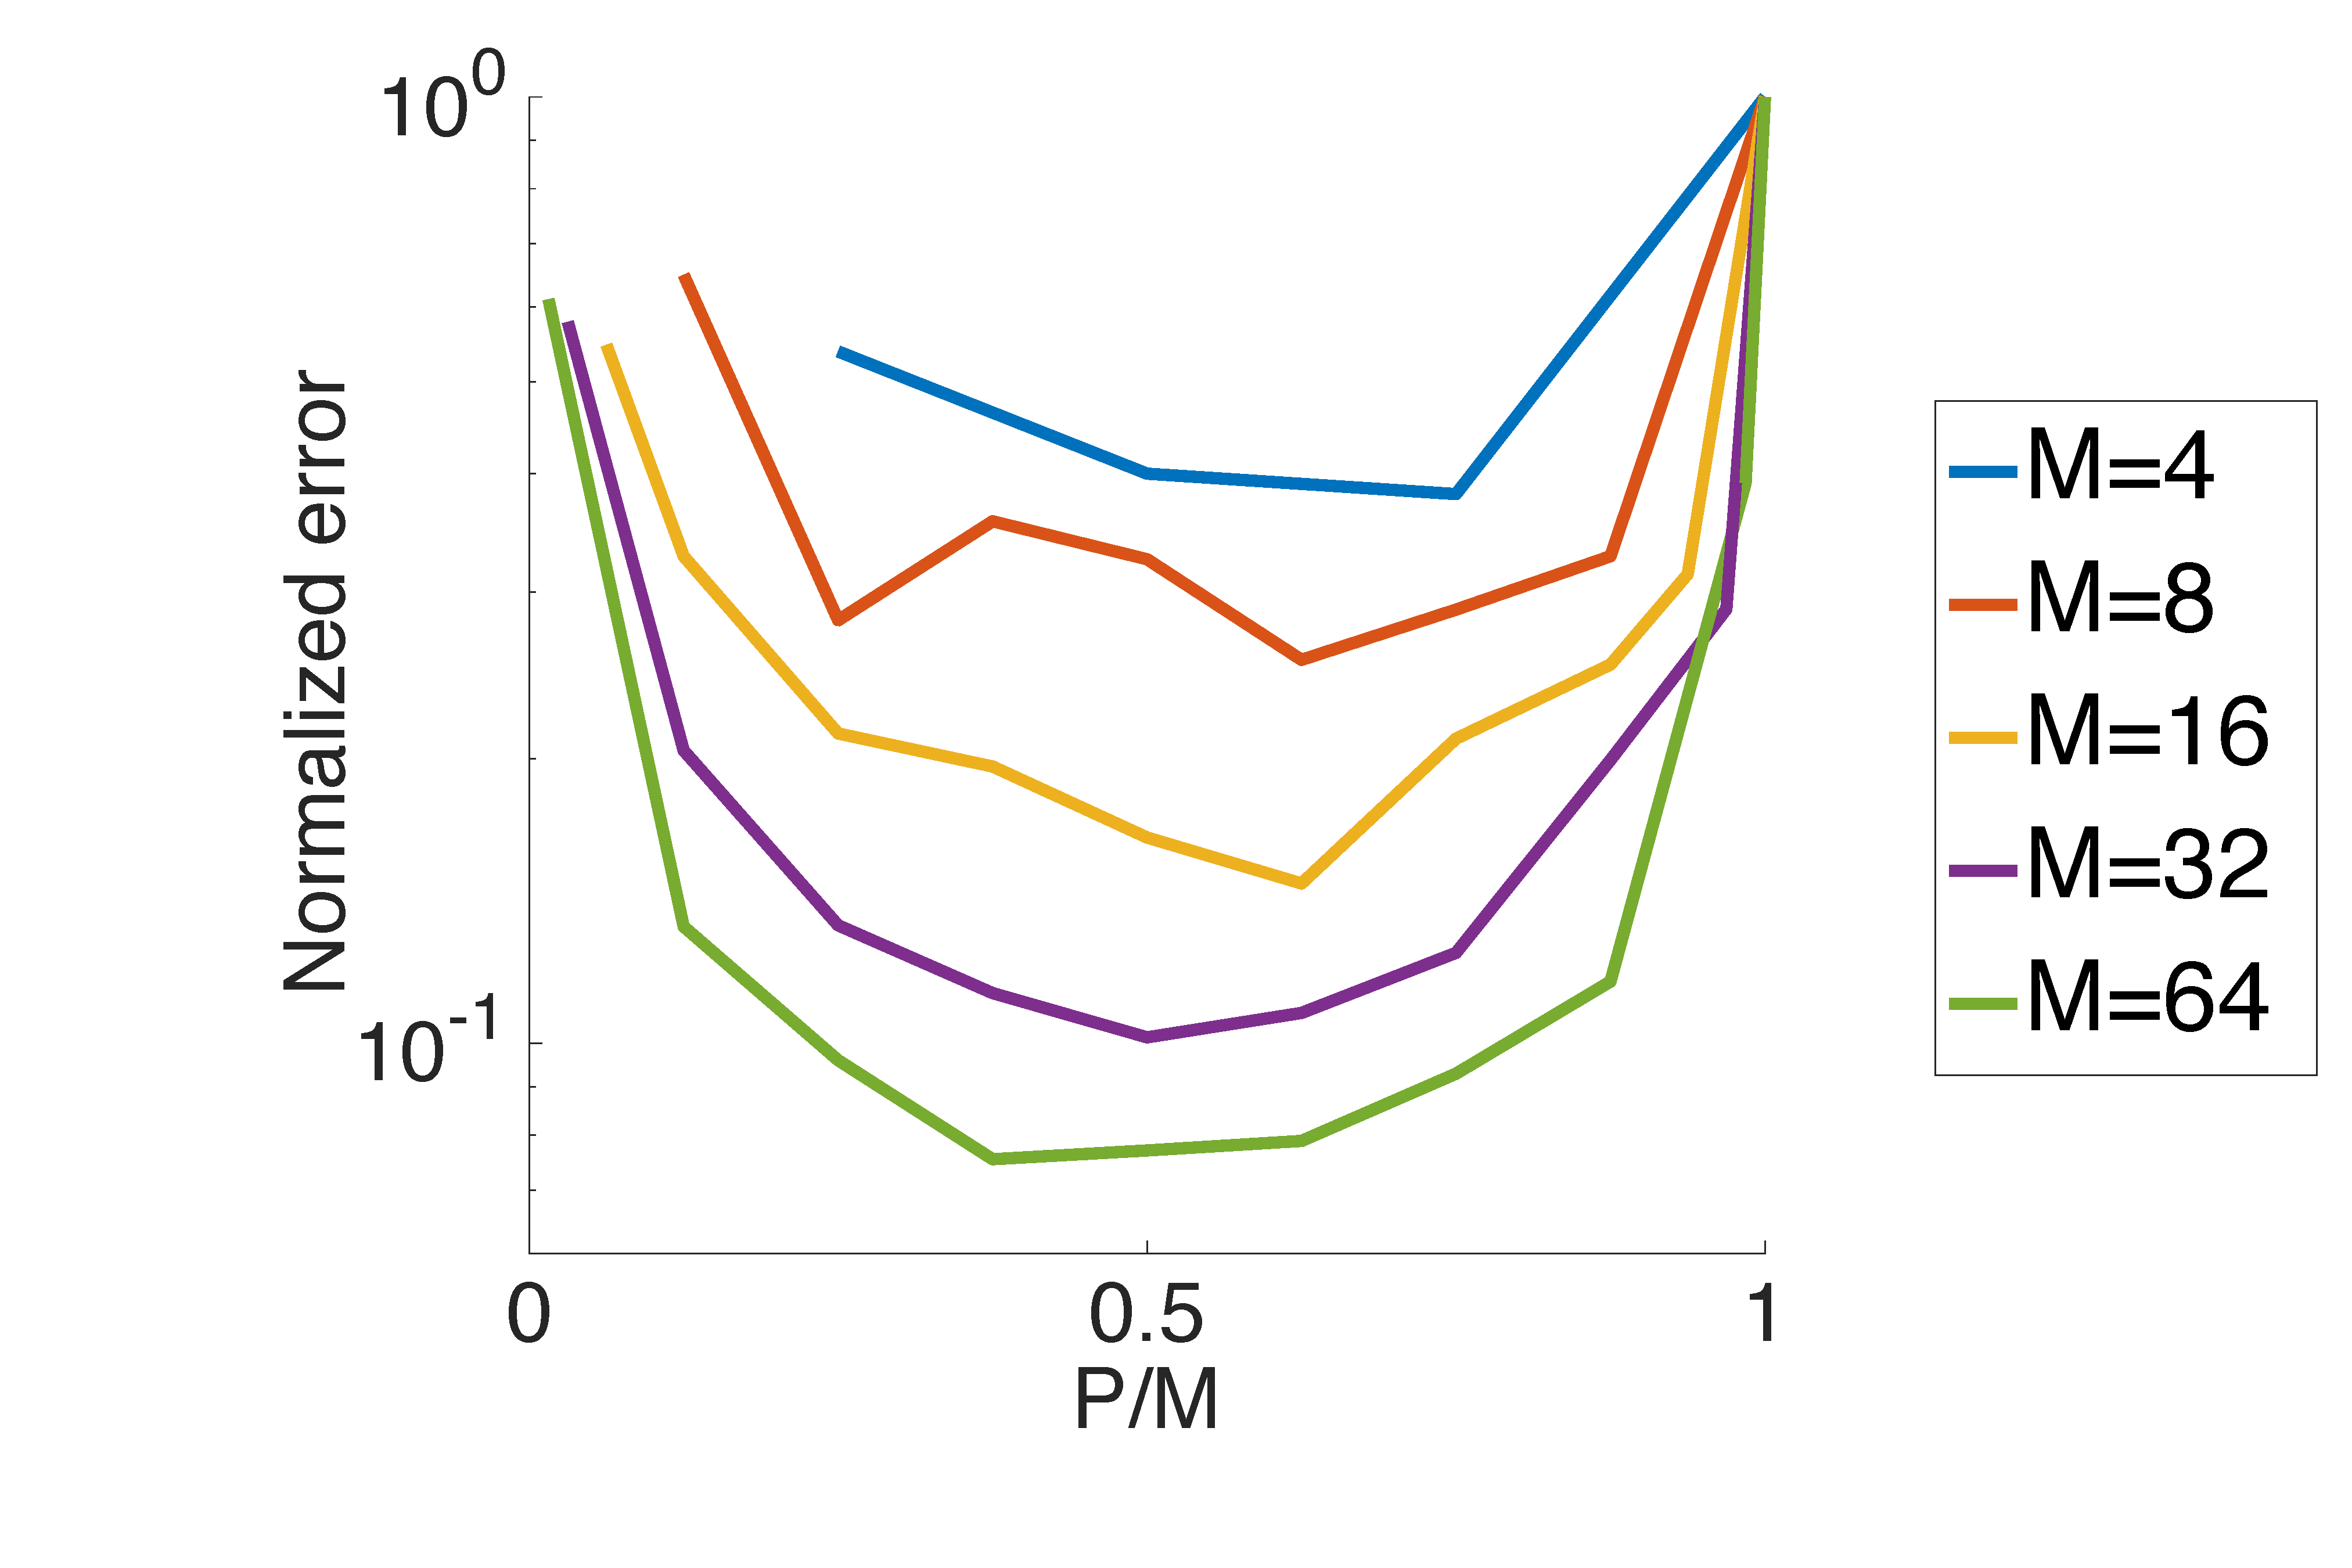
\includegraphics[height=0.75\textwidth]{big_font_p_sweep}
		\caption{Gaussian state space model\label{fig:Psweep}}
	\end{subfigure}
	\vspace{5pt}
	\caption{a) Estimation of switching probability for different choices of P and M assuming the log-Normal limiting distribution for $\hat{Z}_m$ with $\sigma=3$. b) Median error in mean estimate for different choices of P and M over 10 different synthetic datasets of the linear Gaussian state space model given in~\eqref{eq:LGSS} after 1000 MCMC iterations. Here errors are normalized by the error of a multi-start PG sampler which is a special case of iPMCMC for which $P=M$ (see Section \ref{sec:experiments}).
	}
\end{figure}

%
%\begin{figure}[h]
%
%\end{figure}
%~ %add desired spacing 

In practice we also see that best results are achieved when $P$ makes up roughly half of the nodes, see Figure~\ref{fig:Psweep} for performance on the state space model introduced in~\eqref{eq:LGSS}. Note also that the accuracy seems to be fairly robust with respect to the choice of $P$. % At least for this model, three things are clear from this sweep - firstly the optimal choice for the ratio of P/M is roughly 1/2, secondly that the performance of iPMCMC is relatively robust to changes in P around this optimum and thirdly that as $M$ increases, to relatively more preferable iPMCMC is to the trivial distribution of PG given by $P=M$ (this reason this occurs is discussed in more detail in Section \ref{sec:discussion}). 
%
Based on these results, we set the value of $P=M/2$ for the rest of our experiments.

% !TEX root = ../../main.tex

% Numerical experiments section
\subsection{Experiments}
\label{sec:experiments}

To demonstrate the %validity and
empirical performance of iPMCMC we report experiments on two state space models.  
Although both the models considered are Markovian, we emphasise that iPMCMC goes far beyond this and can be applied to arbitrary graphical models. 
%For exposition we will focus our comparison to the trivial distribution, whereby $M$ independent PMCMC samplers are run in parallel, of PG, particle independent Metropolis-Hastings (PIMH) \cite{andrieuDH2010} and the alternate move PG sampler (APG) \cite{holenstein2009particle}. 
We will focus our comparison on the trivially distributed alternatives, whereby $M$ independent PMCMC samplers are run in parallel--these are PG, particle independent Metropolis-Hastings (PIMH) \cite{andrieuDH2010} and the alternate move PG sampler (APG) \cite{holenstein2009particle}. Comparisons to other alternatives, including independent SMC, serialized implementations of PG and PIMH, and running a mixture of independent PG and PIMH samplers, are provided in Appendix \ref{sec:supp-additionalFigures}.  None outperformed the methods considered here, with the exception of running a serialized PG implementation with an increased number of particles, requiring significant additional memory ($O(MN)$ as opposed to $O(M+N)$).

In PIMH a new particle set is proposed at each \mcmc step using an independent \smc sweep, which is then either accepted or rejected using the standard Metropolis-Hastings acceptance ratio. % \cite{andrieuDH2010}. %\cite{hastings1970monte}. 
APG interleaves PG steps with PIMH steps
%, alternating between \csmc updates and a Metropolis-Hastings step with an independent \smc proposal,
in an attempt to overcome the issues caused by path degeneracy in PG.  We refer to the trivially distributed versions of these algorithms as multi-start PG, PIMH and APG respectively (mPG, mPIMH and mAPG). 
We use Rao-Blackwellization, as described in \ref{sec:allparticles}, to average over all the generated particles for all methods, weighting the independent Markov chains equally for mPG, mPIMH and mAPG. We note that mPG is a special case of iPMCMC for which $P=M$.  For simplicity, multinomial resampling was used in the experiments, with the prior transition distribution of the latent variables taken for the proposal.  $M=32$ nodes and $N=100$ particles were used unless otherwise stated.  Initialization of the retained particles for iPMCMC and mPG was done by using standard SMC sweeps.

\subsubsection{Linear Gaussian State Space Model}
\label{sec:LGSS}
We first consider a linear Gaussian state space model (LGSSM) with 3 dimensional latent states $x_{1:T}$, 20 dimensional observations $y_{1:T}$ and dynamics given by %\cn{It seems you use deterministic initial conditions for $x_0$, reformulate the model so you have a prior $\mu(x_1)$ instead? (also follows notation above)}
\begin{subequations}
	\label{eq:LGSS}
	\begin{align}
	x_1 & \sim \mathcal{N} \left(\mu, V\right) \label{eq:LGSSa}\\
	x_t & = \alpha x_{t-1} + \delta_{t-1} \quad & \delta_{t-1} \sim \mathcal{N} \left(0, \Omega\right) \label{eq:LGSSb}\\
	y_t & = \beta x_{t} + \varepsilon_{t} \quad & \varepsilon_{t} \sim \mathcal{N} \left(0, \Sigma\right).
	\label{eq:LGSSc}
	\end{align}
\end{subequations}
We set $\mu = [0, 1, 1]^T$, $V = 0.1 \; \mathbf{I}$, $\Omega = \mathbf{I}$ and $\Sigma = 0.1 \; \mathbf{I}$ where $\mathbf{I}$ represents the identity matrix.  The constant transition matrix, $\alpha$, corresponds to successively applying rotations of $\frac{7\pi}{10}$, $\frac{3\pi}{10}$ and $\frac{\pi}{20}$ about the first, second and third dimensions of $x_{t-1}$ respectively followed by a scaling of $0.99$ to ensure that the dynamics remain stable.  A total of 10 different synthetic datasets of length $T=50$ were generated by simulating from~\eqref{eq:LGSSa}--\eqref{eq:LGSSc}, each with a different emission matrix $\beta$ generated by sampling each column independently from a symmetric Dirichlet distribution with concentration parameter 0.2.

Figure \ref{fig:meanConv} shows convergence in the estimate of the latent variable means to the ground-truth solution for iPMCMC and the benchmark algorithms as a function of MCMC iterations.  It shows that iPMCMC comfortably outperforms the alternatives from around 200 iterations onwards, with only iPMCMC and mAPG demonstrating behaviour consistent with the Monte Carlo convergence rate, suggesting that mPG and mPIMH are still far from the ergodic regime.  Figure \ref{fig:meanPos} shows the same errors after $10^4$ MCMC iterations as a function of position in state sequence.  This demonstrates that iPMCMC outperformed all the other algorithms for the early stages of the state sequence, for which mPG performed particularly poorly. Toward the end of state sequence, iPMCMC, mPG and mAPG all gave similar performance, whilst that of mPIMH was significantly worse.


\begin{figure*}[t]
	\centering
	\begin{subfigure}[t]{0.49\textwidth}
		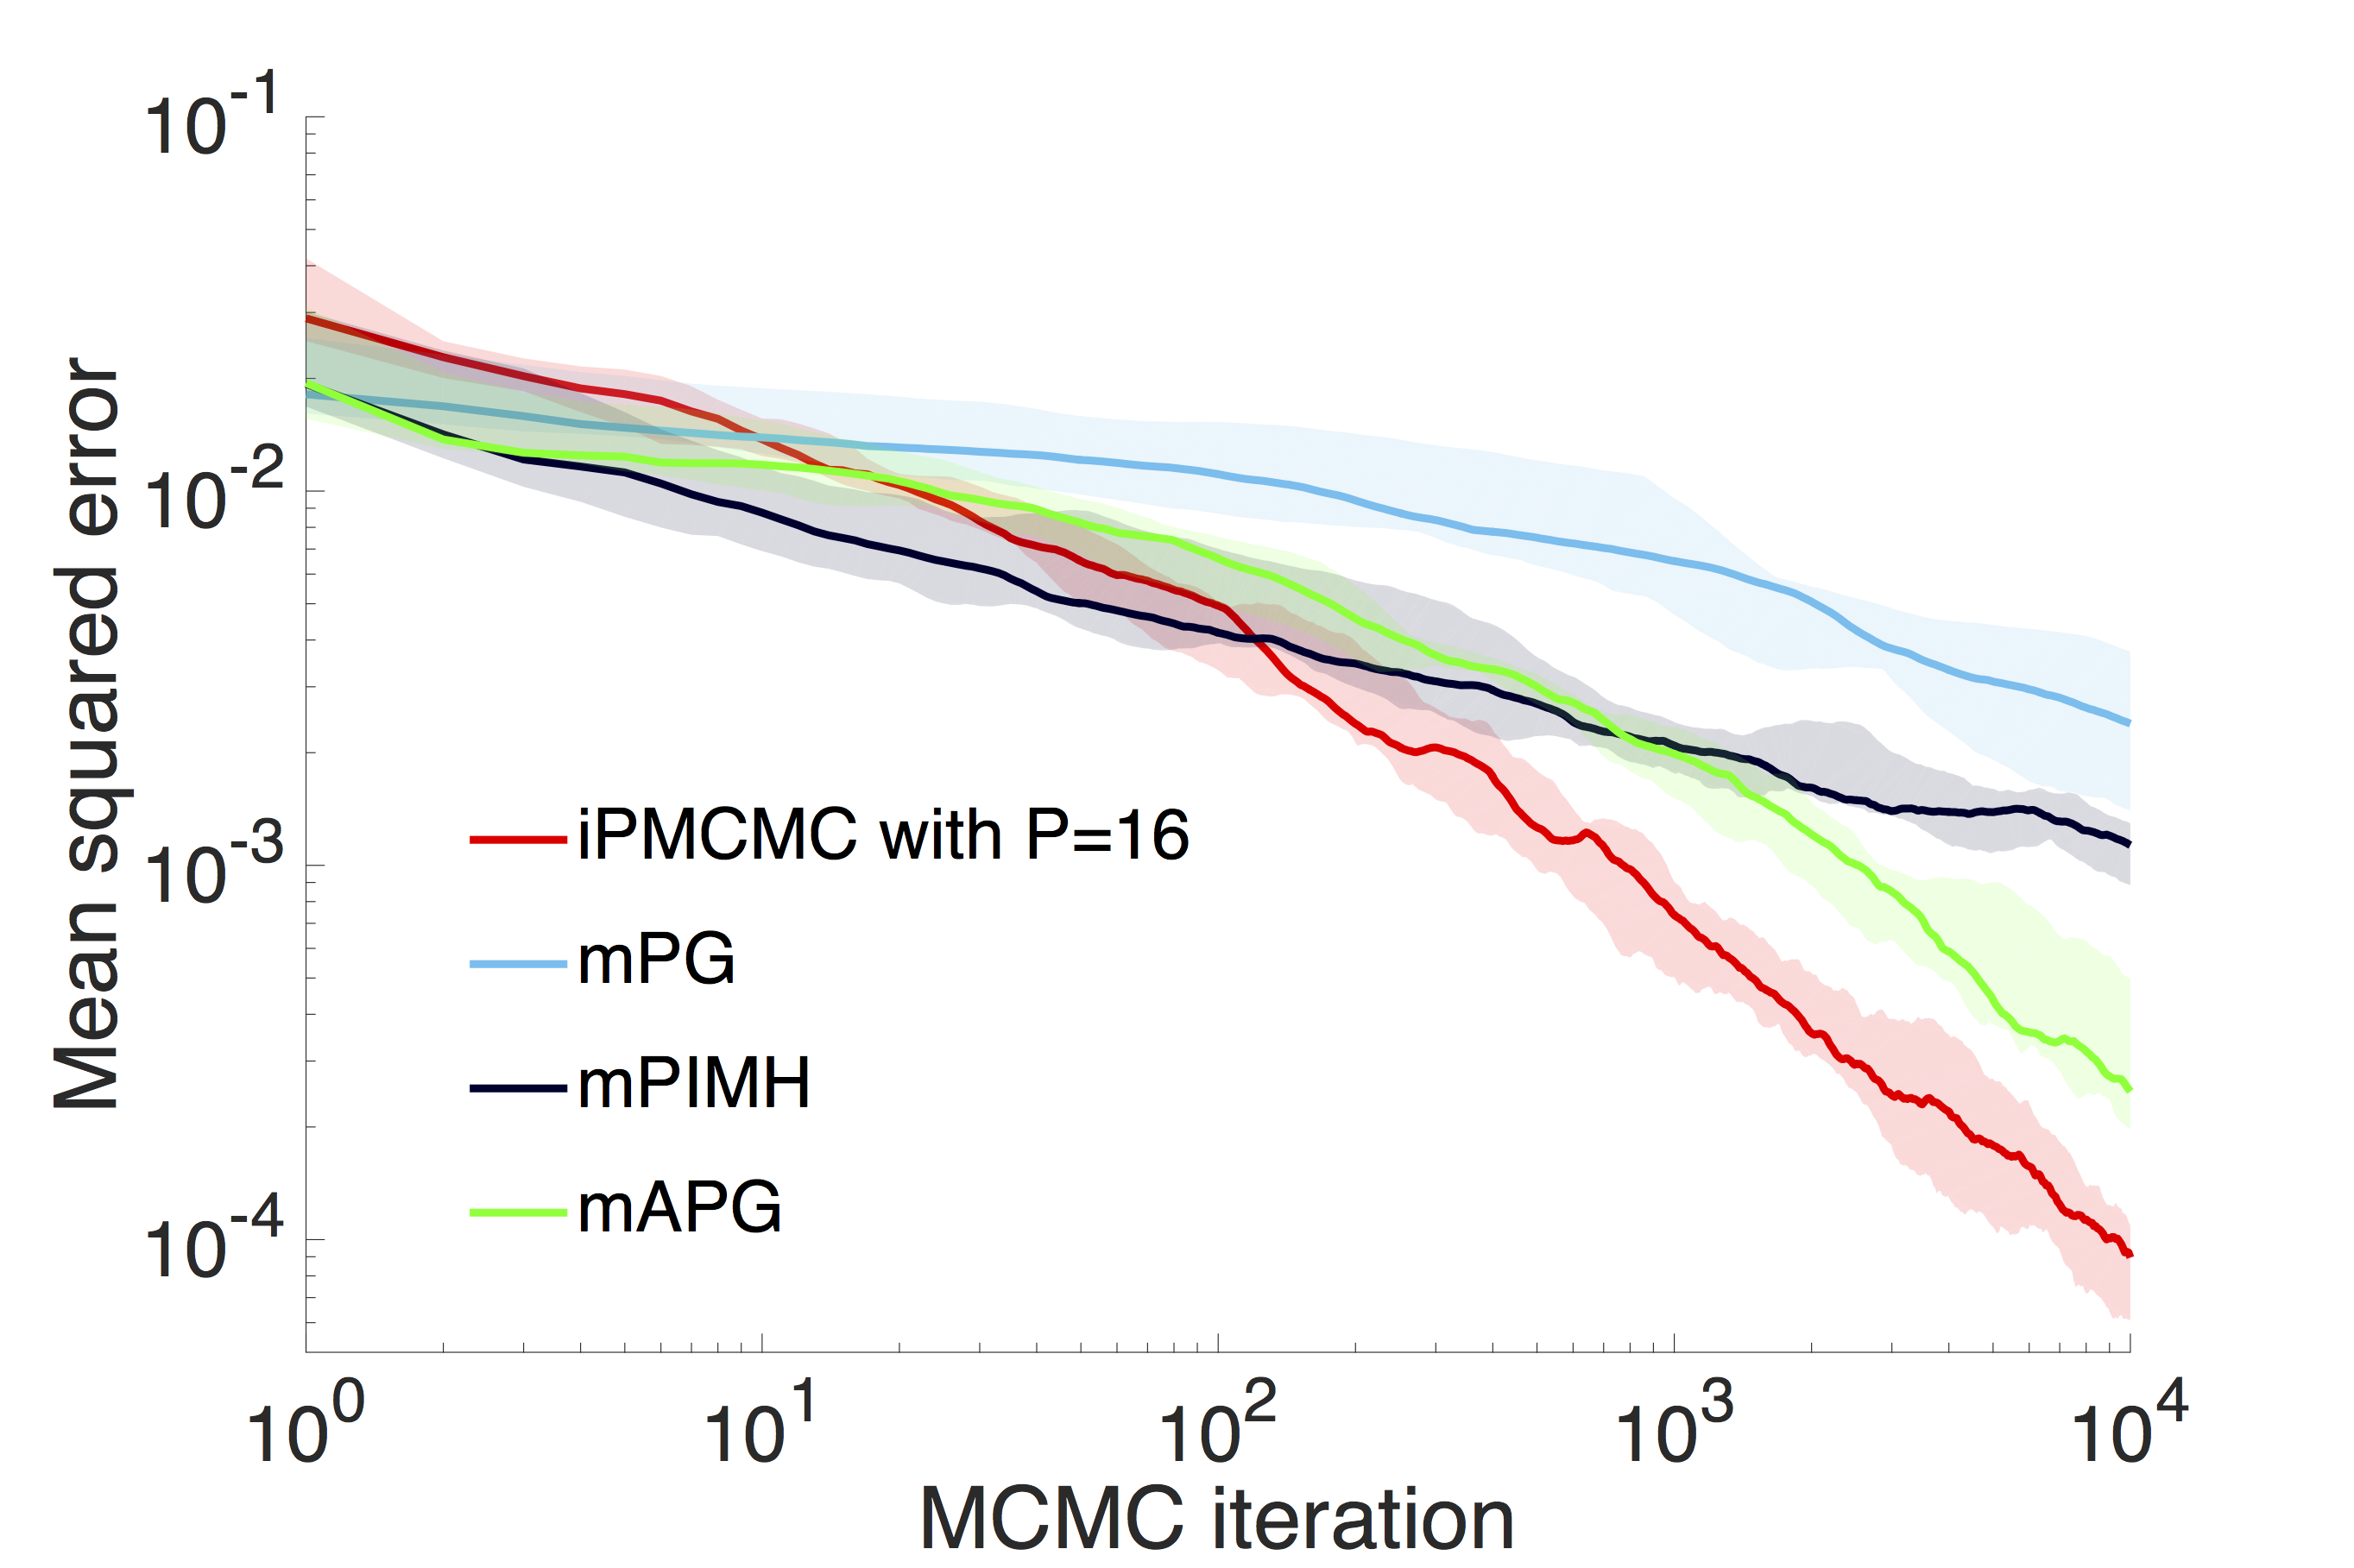
\includegraphics[width=\textwidth]{mean_conv_lss}
		\caption{Convergence in mean for full sequence}
		\label{fig:meanConv}
	\end{subfigure}
	~  %add desired spacing between images, e. g. ~, \quad, \qquad, \hfill etc. 
	%(or a blank line to force the subfigure onto a new line)
	\begin{subfigure}[t]{0.49\textwidth}
		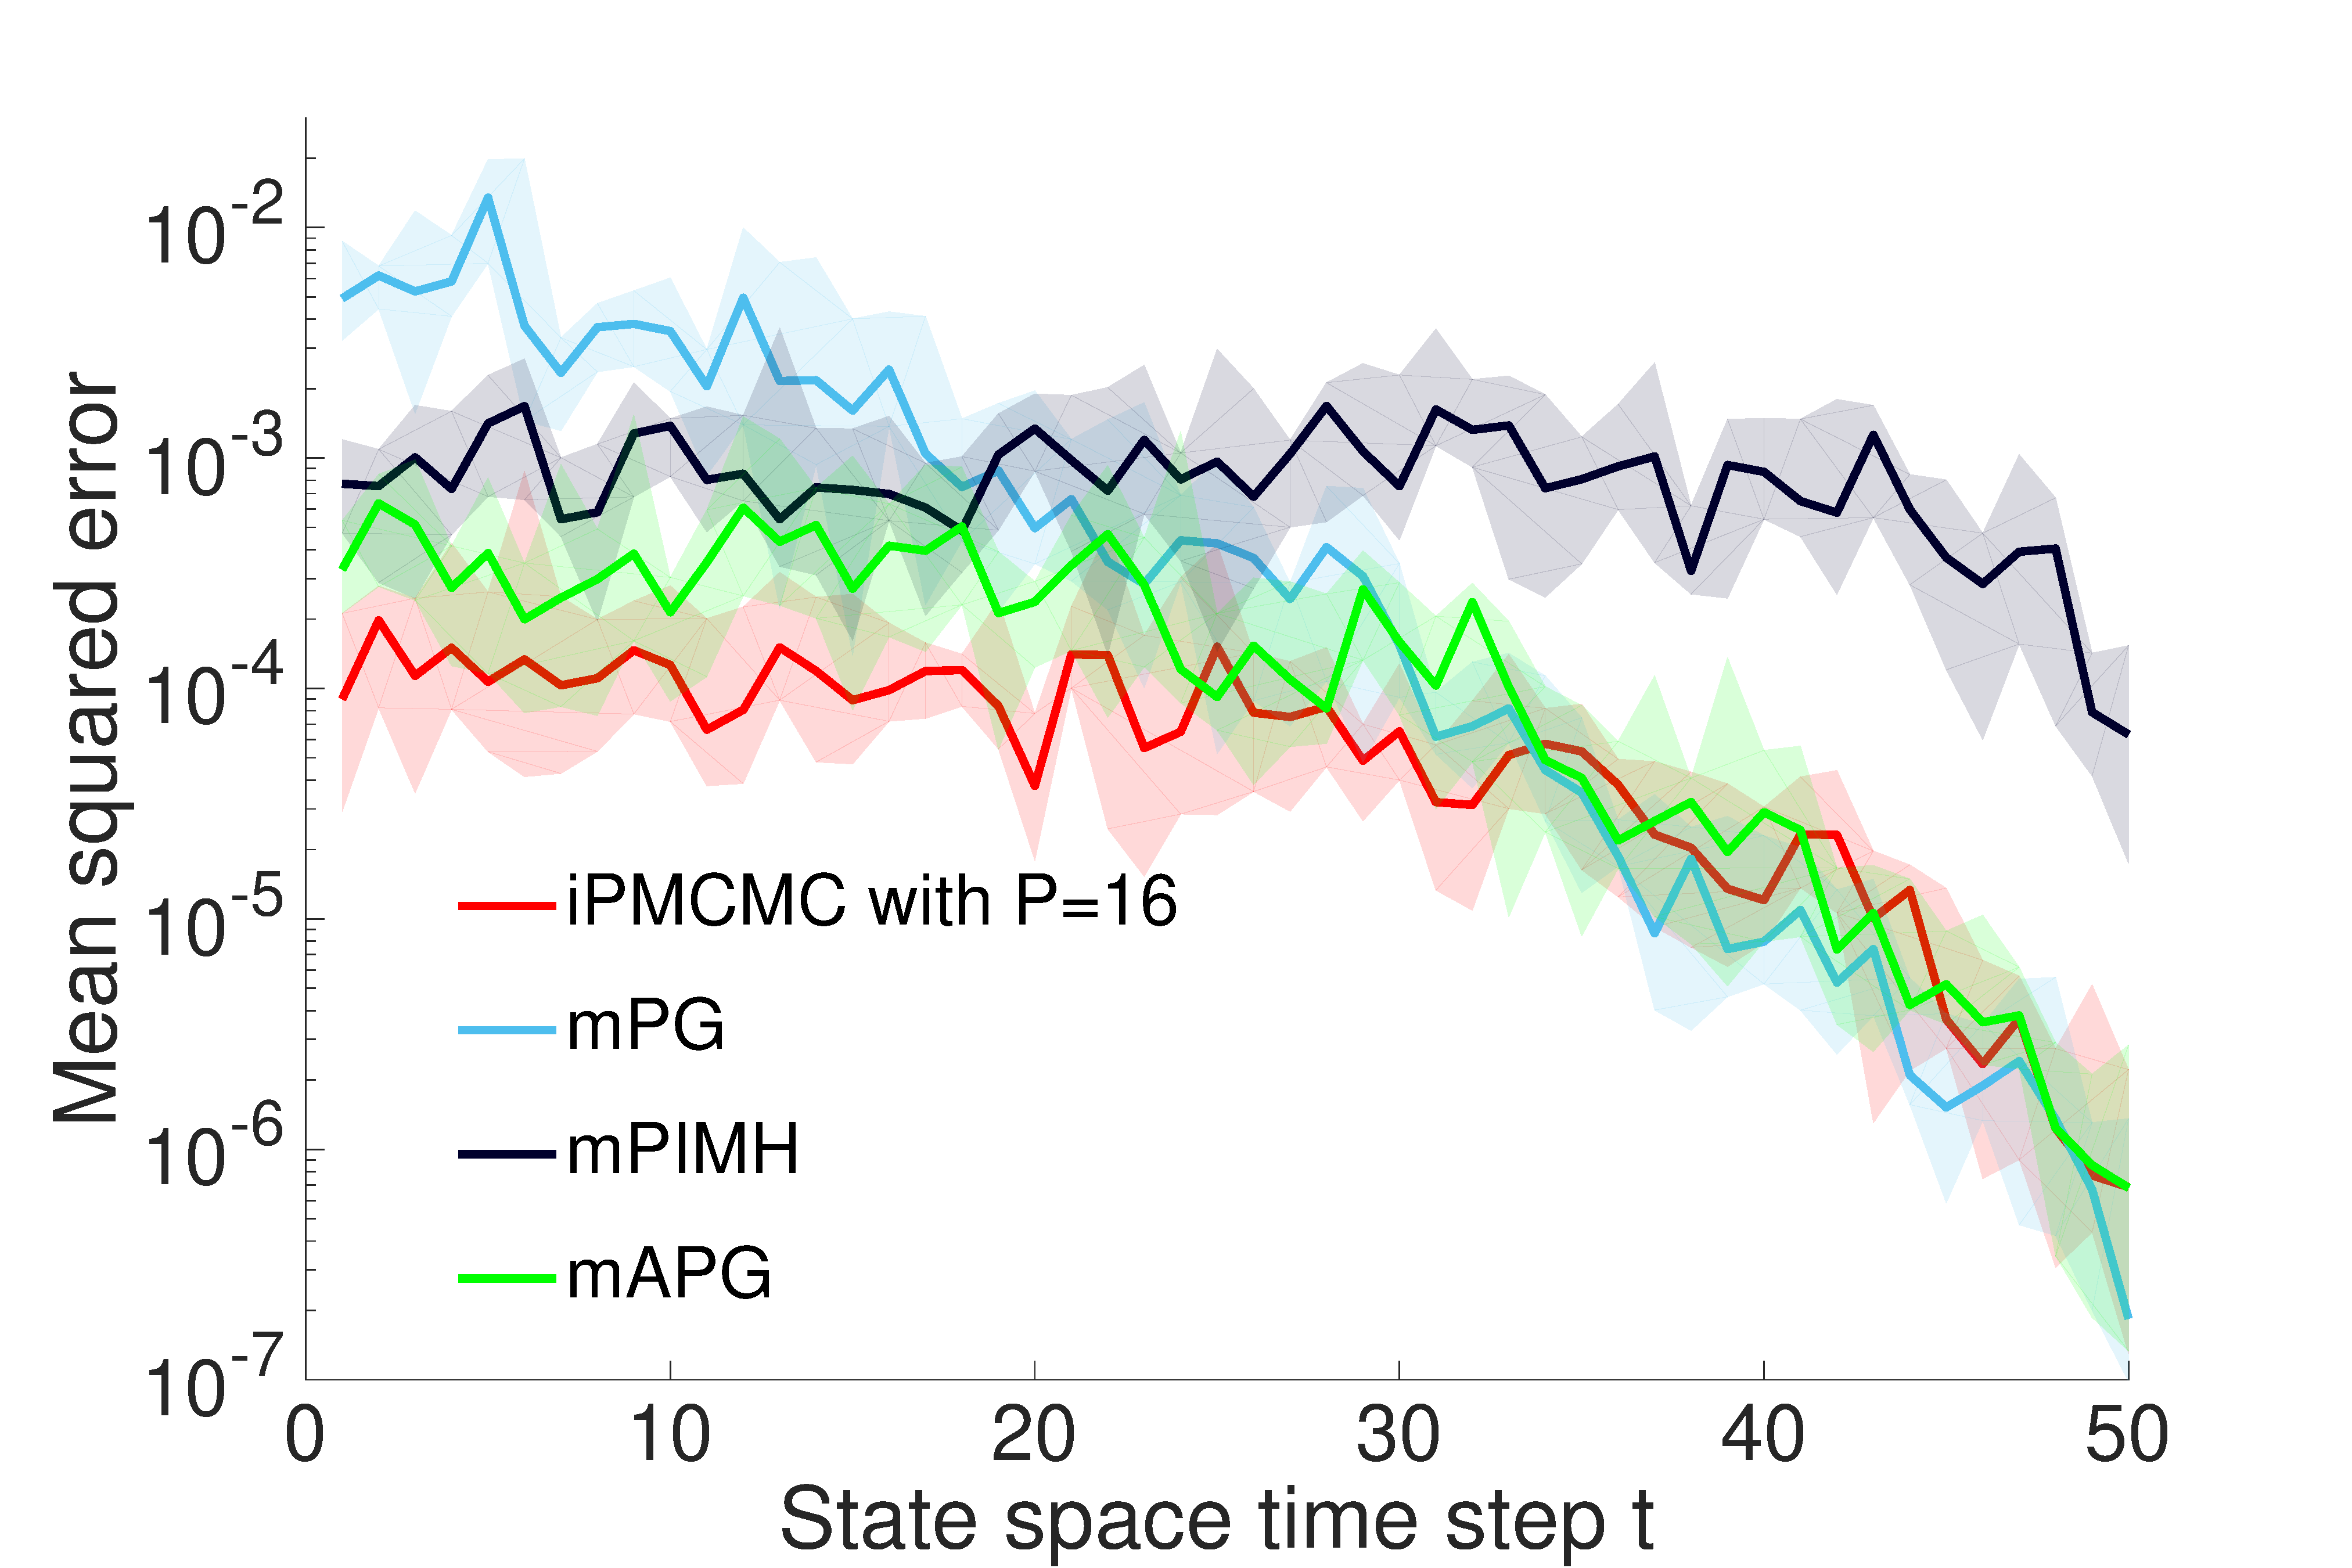
\includegraphics[width=\textwidth]{mean_pos_lss}
		\caption{Final error in mean for latent marginals}
		\label{fig:meanPos}
	\end{subfigure}
	
	%	\begin{subfigure}[t]{0.49\textwidth}
	%		\includegraphics[width=\textwidth]{std_conv_lss}
	%		\caption{Convergence in standard deviation for full sequence}
	%		\label{fig:stdConv}
	%	\end{subfigure}
	%	~ %add desired spacing between images, e. g. ~, \quad, \qquad, \hfill etc. 
	%	%(or a blank line to force the subfigure onto a new line)
	%	\begin{subfigure}[t]{0.49\textwidth}
	%		\includegraphics[width=\textwidth]{std_pos_lss}
	%		\caption{Final error in standard deviation for latent marginals}
	%		\label{fig:stdPos}
	%	\end{subfigure}	
	\caption{Mean squared error averaged over all dimensions and steps in the state sequence as a function of MCMC iterations (left) and mean squared error after $10^4$ iterations averaged over dimensions as function of position in the state sequence (right) for \eqref{eq:LGSS} with 50 time sequences.  The solid line shows the median error across the 10 tested synthetic datasets, while the shading shows the upper and lower quartiles.  Ground truth was calculated using the Rauch--Tung--Striebel smoother algorithm \cite{rauch1965maximum}. 
		\label{fig:groundTruth}}
\end{figure*}

\begin{figure*}[t]
	\centering
	\begin{subfigure}[t]{0.49\textwidth}
		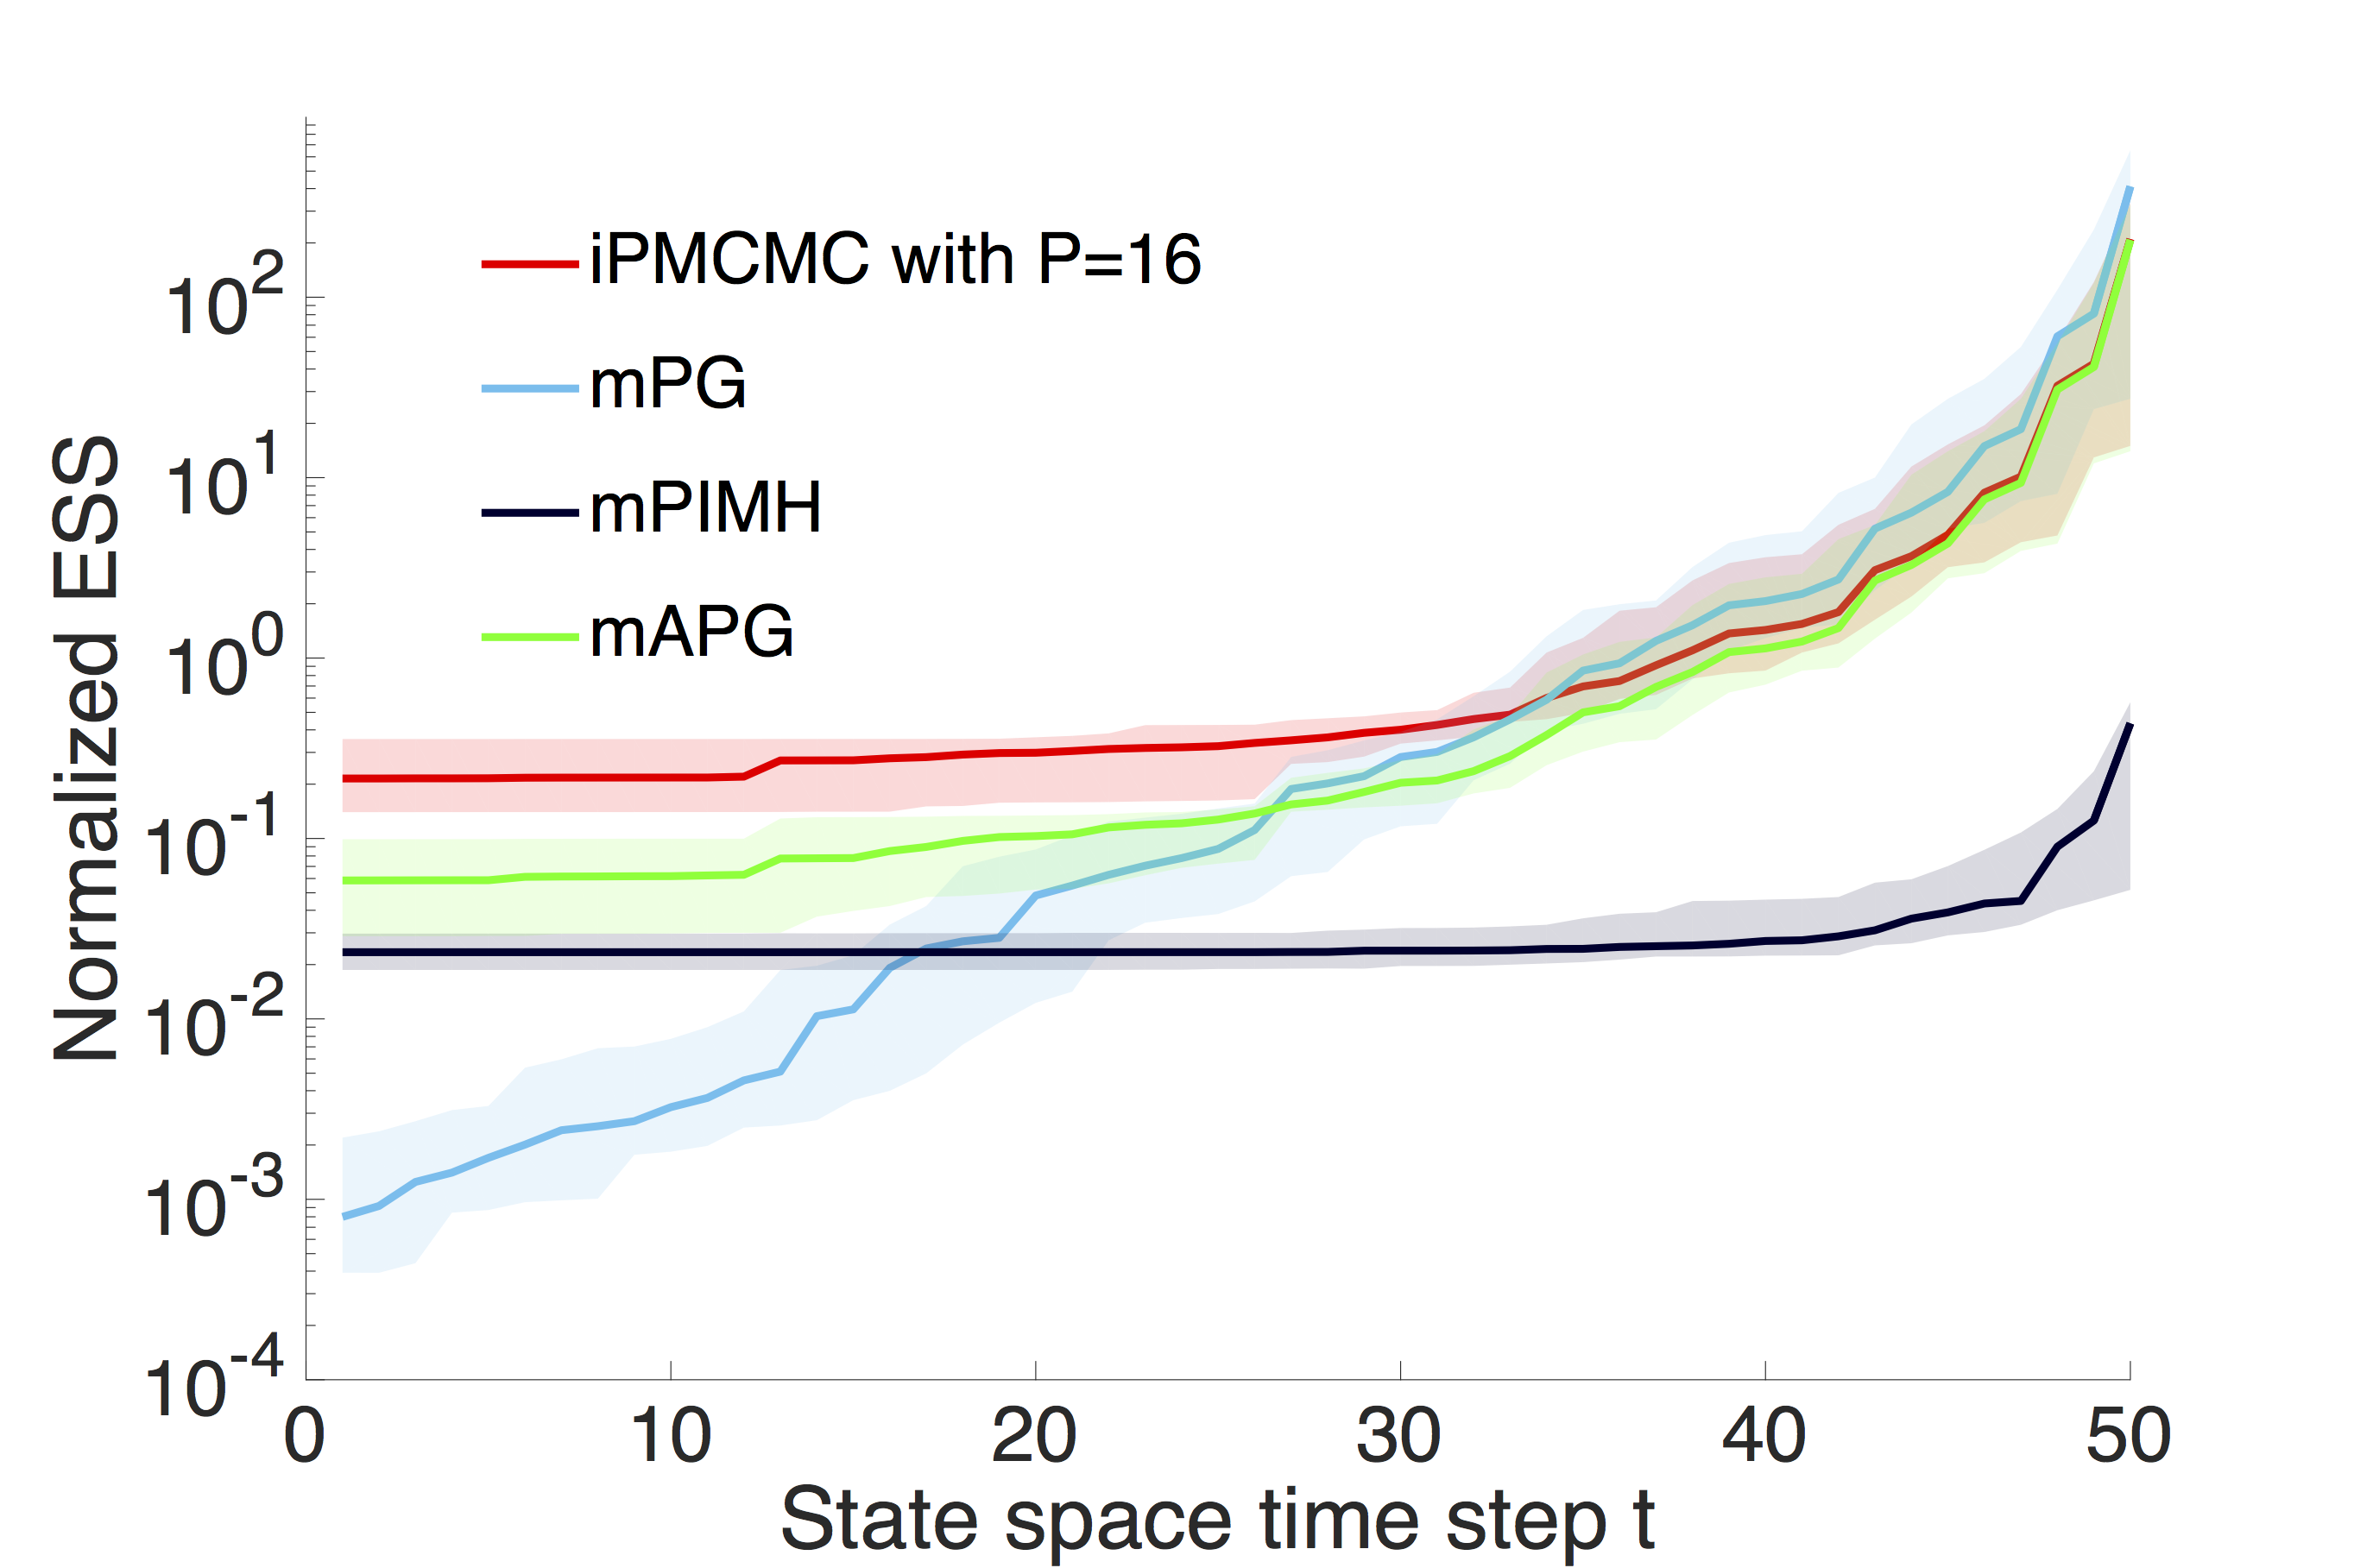
\includegraphics[width=\textwidth]{ess_lss}
		\caption{LGSSM}
	\end{subfigure}
	~ %add desired spacing between images, e. g. ~, \quad, \qquad, \hfill etc. 
	%(or a blank line to force the subfigure onto a new line)
	\begin{subfigure}[t]{0.49\textwidth}
		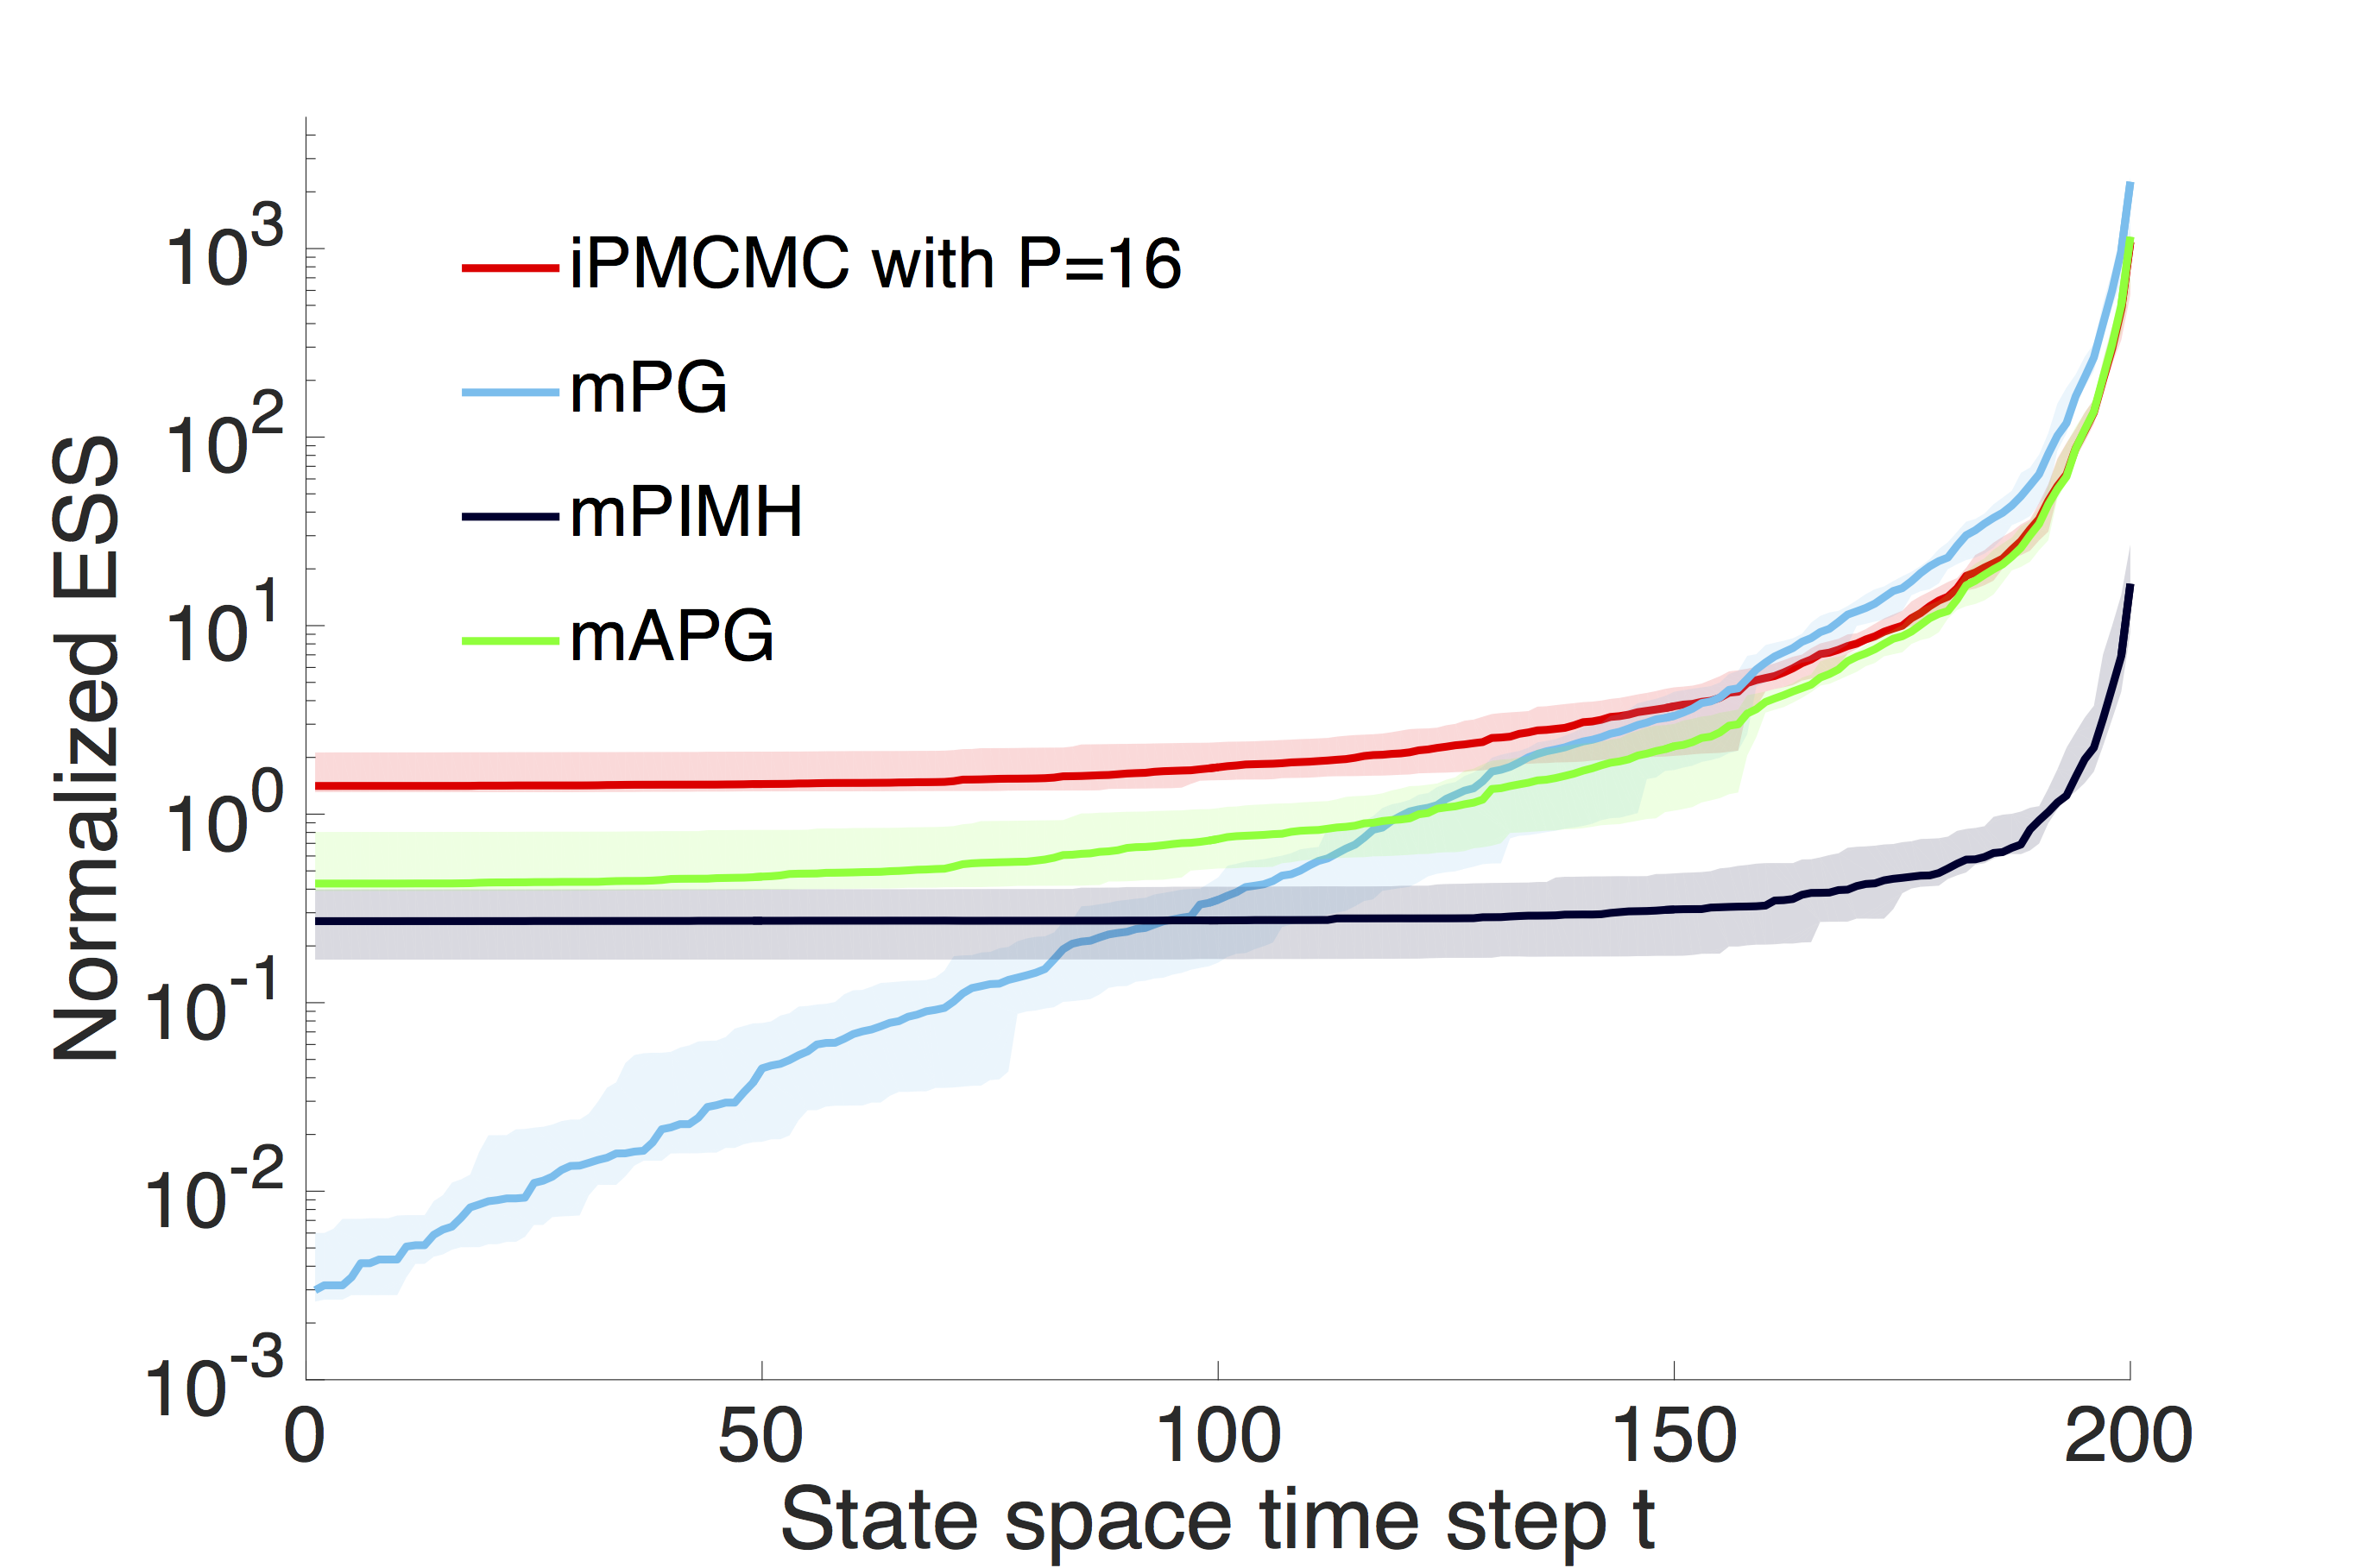
\includegraphics[width=\textwidth]{ess_nlss}
		\caption{NLSSM}
	\end{subfigure}
	
	\caption{Normalized effective sample size  (NESS) for LGSSM (left) and NLSSM (right).
		\label{fig:ESS}}
\end{figure*}

\subsubsection{Nonlinear State Space Model}
\label{sec:nlss}

We next consider the one dimensional nonlinear state space model (NLSSM) considered by, among others, \citet{gordon1993novel,andrieuDH2010}
\begin{subequations}
	\label{eq:NLSS}
	\begin{align}
	x_1 & \sim \mathcal{N} \left(\mu, v^2\right) \label{eq:NLSSa}\\
	x_t & = \frac{x_{t-1}}{2} + 25 \frac{x_{t-1}}{1+x_{t-1}^2} + 8 \cos \left(1.2t\right) + \delta_{t-1} \label{eq:NLSSb} \\
	y_t & = \frac{{x_{t}}^2}{20} + \varepsilon_{t} \label{eq:NLSSc}
	\end{align}
\end{subequations}
where $\delta_{t-1} \sim \mathcal{N} \left(0, \omega^2\right)$ and $\varepsilon_{t} \sim \mathcal{N} \left(0, \sigma^2\right)$.  We set the parameters as $\mu = 0$, $v=\sqrt{5}$, $\omega = \sqrt{10}$ and $\sigma = \sqrt{10}$.  Unlike the LGSSM, this model does not have an analytic solution and therefore one must resort to approximate inference methods. 
% such as sampling.
Further, the multi-modal nature of the latent space makes full posterior inference over $x_{1:T}$ challenging for long state sequences. 

\begin{figure*}[t]
	\centering
	%\begin{subfigure}[t]{0.99\textwidth}
	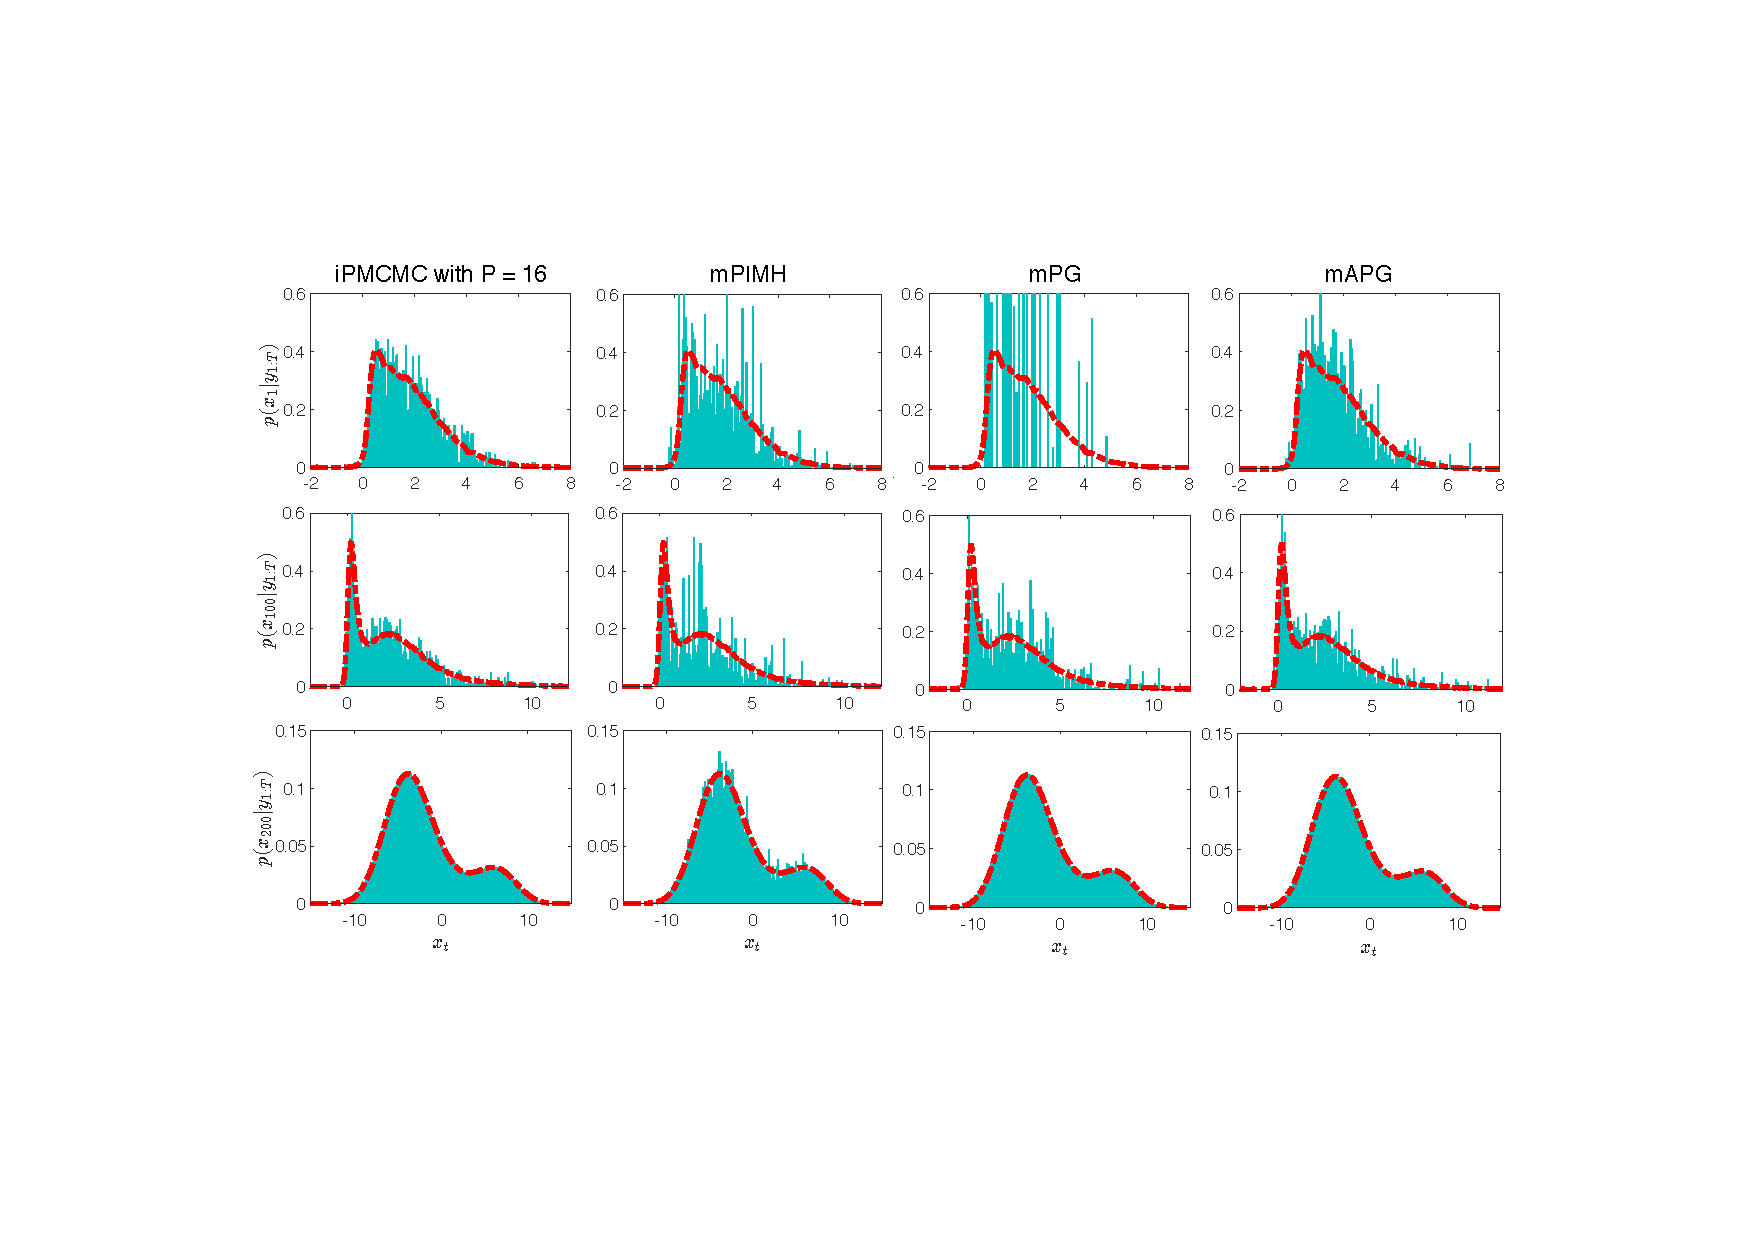
\includegraphics[width=1\textwidth]{nlss_histograms_minus_190.pdf}
	%\end{subfigure}
	\caption{Histograms of generated samples at $t=1, 100, \text{ and } 200$ for a single dataset generated from \eqref{eq:NLSS} with $T=200$.  Dashed red line shows an approximate estimate of the ground truth, found by running a kernel density estimator on the combined samples from a small number of independent SMC sweeps, each with $10^7$ particles. \label{fig:nlssHists}}
\end{figure*}

To examine the relative mixing of iPMCMC we calculate an effective sample size (ESS) for different steps in the state sequence.  In order to calculate the ESS, we condensed identical samples as done in for example \cite{vandemeent_aistats_2015}.  Let 
\begin{align*}
u_{t}^k \in \{x_{t,m}^{i}[r]\}^{i=1:N,r=1:R}_{m=1:M}, \quad \forall k \in 1 \dots K, \; t \in 1 \dots T
\end{align*} 
denote the unique samples of $x_t$ generated by all the nodes and sweeps of particular algorithm after $R$ iterations, where $K$ is the total number of unique samples generated.  The weight assigned to these unique samples, $v_t^{k}$, is given by the combined weights of all particles for which $x_t$ takes the value $u_{t}^k$:
\begin{align}
v_t^{k} = \sum_{r=1}^{R} \sum_{m=1}^{M} \sum_{i=1}^{N} \bar{w}_{t,m}^{i,r} \eta_{m}^{r} \delta_{x_{t,m}^{i}[r]}(u_{t}^{k})
\end{align}
where $\delta_{x_{t,m}^{i}[r]}(u_{t}^{k})$ is the Kronecker delta function and $\eta_{m}^{r}$ is a node weight.  For iPMCMC the node weight is given by as per the Rao-Blackwellized estimator described in Section~\ref{sec:allparticles}. For mPG and mPIMH, $\eta_{m}^{r}$ is simply $\frac{1}{RM}$,
as samples from the different nodes are weighted equally in the absence of interaction. 
Finally we define the effective sample size as $\text{ESS}_t = \left(\textstyle\sum_{k=1}^K \left(v_t^{k}\right)^2\right)^{-1}$.
%\begin{align}
%\label{eq:ESS}
%\text{ESS}_t = \left(\textstyle\sum_{k=1}^K \left(v_t^{k}\right)^2\right)^{-1}.
%\end{align}

Figure \ref{fig:ESS} shows the ESS for the LGSSM and NLSSM as a function of position in the state sequence.  For this, we omit the samples generated by the initialization step as this SMC sweep is common to all the tested algorithms.  We further normalize by the number of MCMC iterations so as to give an idea of the rate at which unique samples are generated.  These show that for both models the ESS of iPMCMC, mPG and mAPG is similar towards the end of the space sequence, but that iPMCMC outperforms all the other methods at the early stages. The ESS of mPG was particularly poor at early iterations.  PIMH performed poorly throughout, reflecting the very low observed acceptance ratio of around $7.3\%$ on average. 
%The lack of Monte Carlo convergence rate appearing in Figure \ref{fig:meanConv} also suggests this acceptance ratio is yet to converge, with the value in the ergodic regime likely to be even lower.   

It should be noted that the ESS is not a direct measure of performance for these models.  For example, the equal weighting of nodes is likely to make the ESS artificially high for mPG, mPIMH and mAPG, when compared with methods such as iPMCMC that assign a weighting to the nodes at each iteration.  To acknowledge this, we also plot histograms for the marginal distributions of a number of different position in the state sequence as shown in Figure \ref{fig:nlssHists}.  These confirm that iPMCMC and mPG have similar performance at the latter state sequence steps, whilst iPMCMC is superior at the earlier stages, with mPG producing almost no more new samples than those from the initialization sweep due to the degeneracy.  The performance of PIMH was consistently worse than iPMCMC throughout the state sequence, with even the final step exhibiting noticeable noise.

%An important feature of the ESS is that it is equal to the total number of samples ($NRM$) if all the samples are unique and have the same weight, and is equal to $1$ if there is only single unique sample with non-zero weight. It should be noted that ESS is not a direct measure of performance in the context of distributed PMCMC methods. In particular it takes no account of the suitability of the weights assigned to samples, for example the equal weighting assigned to different chains for mPG and mPIMH mean they will always have a higher ESS for a particle sweep \brooks{clarify ``particle sweep''?} than a iPMCMC sweep generating the same samples, regardless of whether this equal weighting gives a better approximation to the true posterior. \fredrik{I did not quite understand the last sentence.}

% !TEX root = ../../main.tex

% Discussion for things such as choice of P
\subsection{Discussion}
\label{sec:discussion}

The \ipmcmc sampler overcomes degeneracy issues in \pg by allowing the newly sampled particles from \smc nodes to replace the retained particles in \csmc nodes. Our experimental results demonstrate that, for the models considered, this switching in rate is far higher than the rate at which PG generates fully independent samples. Moreover, the results in Figure~\ref{fig:Psweep} suggest that the degree of improvement over an m\pg sampler with the same total number of nodes increases with the total number of nodes in the pool. 

The mAPG sampler performs an accept reject step that compares the marginal likelihood estimate of a single \csmc sweep to that of a single \smc sweep. In the \ipmcmc sampler the \csmc estimate of the marginal likelihood is compared to a population sample of \smc estimates, resulting in a higher probability that at least one of the \smc nodes will become a \csmc node.

%To explain the benefits of \ipmcmc  over mPIMH and mAPG methods consider a mAPG sampler where the PG and PIMH updates are out of sync for the different nodes such that at any particular MCMC iteration, half of the nodes are applying a PG update and the other half a PIMH update.  One could now informally view the sampling of the retained particles in mAPG as a simplified version of iPMCMC with $P=M/2$, except that the node-weights have been set equally and each of the unconditional SMC sweeps has been arbitrarily assigned as a proposal for one of the CSMC nodes.  Clearly this arbitrary assignment is detrimental as whilst the conditional nodes in iPMCMC consider both themselves and all the of the unconditional nodes for sampling a new retained particle, in mAPG they are restricted to drawing from either themselves or single alternative SMC sweep.  iPMCMC thus, in an informal sense, only requires the lowest of the CSMC node weights to be comparable to the highest of SMC node weights for switching to occur, whereas mAPG requires one of the arbitrary pairings to be comparable.  We therefore recommend setting $M$ as higher as possible, potentially even beyond the level of distribution available, noting the performance improvements of serialized PG shown in the supplementary material.



%Whenever PG degenerates to a single particle, this is guaranteed to correspond to the retained particle.  Therefore PG requires multiple particles to be retained from the start of the state sequence in order to generate new unique samples for all the latent variables in an MCMC iteration, causing it to become stuck at the same sample for variables early in the state sequence.  To quantify this improvement we note that $14.9\%$ of the retained particles produced by the iPMCMC sampler (after a short burn-in period), originated from unconditional SMC sweeps at the previous iteration.  Further, on average $85.4\%$ of the MCMC iterations for iPMCMC generated new retained particles for all stages of the state sequence. This contrasts with each PG sampler in mPG case producing an entirely new retained particle at a rate of only $0.076\%$.

%To explain the benefits of iPMCMC over mPIMH and mAPG consider a mAPG sampler where the PG and PIMH updates are out of sync for the different nodes such that at any particular MCMC iteration, half of the nodes are applying a PG update and the other half a PIMH update.  One could now informally view the sampling of the retained particles in mAPG as a simplified version of iPMCMC with $P=M/2$, except that the node-weights have been set equally and each of the unconditional SMC sweeps has been arbitrarily assigned as a proposal for one of the CSMC nodes.  Clearly this arbitrary assignment is detrimental as whilst the conditional nodes in iPMCMC consider both themselves and all the of the unconditional nodes for sampling a new retained particle, in mAPG they are restricted to drawing from either themselves or single alternative SMC sweep.  iPMCMC thus, in an informal sense, only requires the lowest of the CSMC node weights to be comparable to the highest of SMC node weights for switching to occur, whereas mAPG requires one of the arbitrary pairings to be comparable.  We therefore recommend setting $M$ as higher as possible, potentially even beyond the level of distribution available, noting the performance improvements of serialized PG shown in the supplementary material.

%Referring back to Figure~\ref{fig:Psweep}, we see that as $M$ is increased, the better the relative performance of iPMCMC.  As the reported errors are as a proportion of error given by mPG with the same $M$, this improvement is not simply because more computational resources have been allocated, but because the ``pool" from which the retained node indexes can be draw increases.  As the distribution in the ratio of CSMC node weights to SMC node weights is independent of $M$, the probability that all of the retained particles at the next MCMC iteration originate from the CSMC sweeps diminishes as shown by INSERT REF DEPENDING ON WHETHER IN SUP OR SEC XX.  The resulting improvement in performance with increasing $M$ seen in Figure~\ref{fig:Psweep} thus verifies the benefits from the increase interaction provided by iPMCMC.

Since the original \pmcmc paper in 2010 there have been several papers studying \citep{chopin2015,lindsten2015uniform} %\fredrik{Should we give some references to theoretical work on PG? for instance, I know of a paper in SJOS which is very good ;)}
and improving upon the basic \pg algorithm. Key contributions to combat the path degeneracy effect are backward simulation \citep{whiteley2010efficient,lindsten2013backward}
and ancestor sampling \citep{lindstenJS2014}. These can also be used to improve the \ipmcmc method ever further.  

%Noting that the Gibbs update in \eqref{eq:simConditional} requires no interaction between the \csmc nodes, iPMCMC should be amenable to an asynchronous adaptation under the assumption of a random execution time, independent of $\xb'$, in Algorithm~\ref{alg:csmc}.

%For this one would run a number of \smc nodes independently, communicating only their normalisation constant estimate and a sampled trajectory to a pool of possible retained particles with associated weights.  Whenever a \csmc sweep finishes its execution, it samples a new retained particle from either the pool or itself, replenishing the pool with a new sample if the new retained particle was not from the original \csmc sweep.  It should be noted that as this pool could be increased indefinitely, this adaptation has the potential to increase the scope and potential performance of iPMCMC even further.



% MOVED BACK TO METHODS
% Use backward sampling and/or ancestor sampling
%\subsection{Backward Simulation and Ancestor Sampling}
%Adding a backward or ancestor simulation step can drastically increase mixing when sampling the conditional trajectories $\xb_j'[r]$ \citep{lindsten2013backward}. In the \ipmcmc sampler we can replace simulating from the final weights on line~7 by a backward simulation step. Another option for the \csmc nodes is to replace this step by internal ancestor sampling \citep{lindstenJS2014} steps and simulate from the final weights as normal.


\section{Other Methods and Extensions}

\begin{itemize}
	\item Backwards / ancestral sampling
	\item Resample-move stuff
	\item Rejuvenation
\end{itemize}
% !TEX root = ../main.tex

\chapter{General Purpose Inference for Probabilistic Programs}
\label{chp:proginf}

In Chapter~\ref{chp:probprog} we showed how probabilistic programming systems (PPSs) provide
an expressive framework for specifying probabilistic models.  We now consider the other major component
for PPSs: automating inference for any model the user is allowed to specify using general purpose
inference engines.  For most PPSs this requires two things --  a compiler to convert the \emph{query} to an
suitable form for input to the inference engine and the inference engine itself.  

For the inference
driven systems discussed in Section~\ref{sec:probprog:two:inf}, the inference engine typically comprises of
a standard Bayesian inference method for graphical models such as those discussed in Chapters~\ref{chp:bayes}
and~\ref{chp:part}.  Developing these in a way to robustly work for a wide range of problems typically
requires careful engineering and algorithmic innovation -- e.g. because many inference methods require the definition of
a proposal, upon which performance can critically depend -- but does not generally require development 
of approaches distinct to those used outside a probabilistic programming context.  In these 
systems the inference algorithm(s) is/are usually chosen first, with the language and its restrictions built around it.
Therefore the challenges of the designing the system are generally rooted in generalizing and increasing the robustness of the 
specific inference method(s) used.  Similarly, the language itself and associated compiler is generally built
around providing the easiest representation to work with the target model class, while the fact that most of
these such systems to not support higher order functions usually substantially simplifies the compilation
process.

Because the design of these systems is very much driven by the particular inference algorithm used, it
beyond the scope of this thesis to do the associated literature justice.  Our focus will instead mostly be on 
conducting inference for universal PPSs, though some of what we introduce will apply to both.
Unfortunately, we will find that there are very few (known) inference
methods which can actually cope with the most general possible models as we introduced in
Section~\ref{sec:probprog:models:general}, all of which suffer particularly badly from the curse of
dimensionality.  Consequently, it will be necessary to make certain (mostly very small) concessions in 
generality to achieve any reasonable performance on non-toy models.  We will focus on conducting
inference in Anglican~\citep{wood2014new,tolpin2016design} to give us a basis for explanation, but much of
what we discuss will be still be relevant to other universal systems, in particular those which
are also based around \sample-\observe syntax, such as VentureScript~\citep{mansinghka2014venture}, 
WebPPL~\citep{goodman_book_2014}, and Probabilistic C~\citep{paige2014compilation}.

% !TEX root = ../main.tex

\section{Compiling Queries}
\label{sec:proginf:comp}

Non-probabilistic languages can be either compiled, whereby high-level source code
is converted to a lower level language (e.g. byte-code) before being evaluated, or interpreted,
whereby an interpreter reads the program and directly evaluates it based on the language
semantics.  Other than some earlier systems that were based around guess-and-check 
type strategies, PPLs by construction tend to require some form compilation due to the fact that
the original code will typically run many times and because they tend to be integrated
with an existing language, such that they generally require compilation to the host language
before anything can be run.  Rather than just being a technical hurdle, compilation is also 
often an important tool in the ability of probabilistic programming systems to perform
effective inference as it can often be used to establish helpful salient features in the model,
such as dependency structures, variable types, and features of the model that can guide
which inference algorithm is likely to be most successful or even elements of the model
that can be calculated analytically.  Hakaru~\citep{narayanan2016probabilistic} is a good
example of what can be achieved in probabilistic programming through compilation alone,
as it, for example, uses the computer algebra system Maple to automatically simplify models
when possible.

\subsection{What do we want to Achieve through Compilation?}
\label{sec:proginf:comp:want}

So what are the aims of our PPL compiler?  First and foremost, we need to
perform a source-to-source transformation of the program to
produce some representation in the conventional programming language in which
the inference engine is written so that execution of the program is possible and inference
can be carried out.  As a simple example, consider the case of an Anglican program where
we wish only to run importance sampling using the generative model as a proposal 
(i.e. the query with all the\observe statements removed).  Here we need only produce a Clojure program
that samples directly from the generative model and accumulates weights from the
\observe terms as a side-effect.  We can then rerun this program arbitrarily many
times, each returning a sampled output and accompanying weight, to produce a sequence
of importance samples which can then be used to make consistent Monte Carlo estimations.
Such a strategy would be na\"{i}ve though as we would be able to use our Clojure program
for little else than importance sampling with this particular proposal.  Clearly, we want
to compile to a more general purpose representation that permits a wider array inference algorithms
and proposals, and which ideally allows features of the model, such as its dependency
structure, to be exploited.

One desirable feature of our compiled representation is an ability to make partial
program evaluations.  This will allow us to re-evaluate elements of the program in
isolation in a Gibbs sampling style fashion and it will allow us to interrupt the execution
of the program, giving us the ability to add in things such as the resampling step in SMC.
Supporting partial evaluation can also allow us to avoid gratuitous re-executions of
elements of the program whose result is already known by using databases to store and
recall the effect of previous executions.

Another desirable feature is to avoid being restricted to only directly sampling from \sample
statements.  We may wish to sample from a different distribution as a proposal or to evaluate
the probability density of the \sample statement producing a particular output, e.g. as part
of an acceptance ratio calculation for an MCMC scheme.  The key requirement for both of these
is the knowledge of density function associated with the \sample statement, rather than
just access to a black-box sampling scheme.  This is the motivation behind why we defined
the syntax of \sample as taking as input a distribution object which encodes both the density
function and means of sampling from that density.

It will also often be helpful for our compiler to delineate between probabilistic and deterministic
elements of the code.  Other than potentially trying to make efficiency gain by avoiding
repeated computation, we know that any deterministic parts of our code (namely code in between
consecutive \sample and/or \observe statements) can be safely run without the need
to worry about the implications this has on the inference.  The execution of these segments of
the program in isolation can thus be per the language being compiled to, without needing to
worry about the probabilistic semantics.  On the other hand, we will generally desire the identification
of \emph{checkpoints} for positions in the program where \sample or \observe statements are
made so that the behavior of the program at these points can be handed over to the inference
engine.

The compiler will in general also play an important role in the interaction between the PPL
as its integrated language on the behalf of the user.  Any PPL that does not provide produce
outputs in a helpful form that can be manipulated by the user will be somewhat impractical,
while for general purpose systems it is essential to allow the user to link in external 
deterministic code packages specific their particular problem.

This example list of desirable features for our compiler is far from exhaustive.
In particular, there will be many inference specific features required for some
systems, such as the need to have a representation of the derivations, e.g. calculated
through automatic differentiation~\cite{baydin2015automatic}, to carry out 
Hamiltonian Monte Carlo inference~\cite{carpenter2015stan}
or common variational inference methods~\citep{kucukelbir2015automatic}.  As we
said earlier, we will often also want our compilation to, when possible,
pick out salient features of the model, carry out simplifications, and even automatically 
establish the most suitable inference algorithm for a particular problem.  The compiler
is an integral part of any PPL and there is no one best approach for all situations. 
One of the key distinguishing features between different PPLs is how they approach
this compilation problem, with different design choices inevitably lead to systems
geared towards different models or inference algorithms. 

\subsection{Compilation of Anglican Queries}
\label{sec:proginf:comp:ang}

As it is inevitably infeasible to detail the inner workings of a PPL compiler in a general
manner, we now provide a more in depth introduction to compilation method
employed by Anglican.  Our introduction is inevitably not exhaustive, focusing more on
intuition than being exactly true to the implementation details; we refer the reader
to~\citep{tolpin2016design} for a more complete and rigorous introduction.

As we explain in Section~\ref{sec:probprog:anglican:models},
Anglican programs, or queries, are compiled using the macro \query which provides a
Clojure function that can be passed to one of the provided inference algorithms.
The key element of this compilation for providing the desirable properties discussed
in the last section and a convenient interface for the inference algorithms is that
Anglican compiles queries to \emph{continuation passing style} (CPS)~\citep{appel1989continuation}
Clojure functions.\footnote{WebPPL also does a CPS style transformation, 
	namely to a purely functional subset of Javascript.}
At a high level, a continuation is a function that represents the rest of the
program.  CPS is a style of functional programming that uses a series of continuations
to represent the program through a series of nested function calls, where the program
is run by evaluating each function and then passing the output to the continuation
which invokes the rest of the program.  This is perhaps easiest to see through
example.  Consider the simple function \clj{+}, which in Clojure has syntax \clj{(+ a b)}.  The
CPS transformed version of \clj{+}, which we will call \clj{+&} takes an extra input
of the continuation $\mP$ and invokes it after evaluation such that we have
\clj{(defn +& [a b } ~$\mP$\clj{] (}$\mP$ \clj{(+ a b)))}.  More generally, for any simple function \clj{f}, we have
that its the CPS transformation is \clj{(defn f& [args} ~$\mP$\clj{] (}$\mP$ \clj{(f args)))}.\footnote{Note that
	in practice, the continuation is usually set to be the first argument in order to provide support
	for functions with a variable number of inputs.}
  We 
will use this notation of adding an \clj{&} to an expression name to denote its CPS transformation throughout.
To give a more detailed example, the CPS transform of the program \clj{(max 6 (* 4 (+ 2 3)))} would be
\begin{lstlisting}[basicstyle=\ttfamily\small,frame=none]
  (fn [$\mP$] (+& 2 3 (fn [x] (*& 4 x (fn [y] (max& 6 y $\mP$)))))
\end{lstlisting}\vspace{-8pt}
where \clj{*&} and
\clj{max&} are analogous to \clj{+&} defined as before.
Here our first continuation is \clj{(fn [x] (*& 4 x (fn [y] (max& 6 y))))} and our second continuation 
is \clj{(fn [y] (max& 6 y))}.  Note that the CPS transformed code is itself a function because
it itself takes a continuation.  

Things are a little
trickier for general expression that are neither literals nor simple first order functions, for example,
binding forms like \clj{let}, Anglican special forms like \sample, and branching statements like \clj{if}.
For these expressions, the high-level idea is the same, but the CPS transformation is, unfortunately, 
expression specific and must, in general, be implemented on a case-by-case basis.  
For example, one can CPS transform \clj{let} by going from
\clj{(let [x (foo1 1) y (foo2 2)] (foo3 x y))} to
 \begin{lstlisting}[basicstyle=\ttfamily\small,frame=none]
 (fn [$\mP$] (foo1& 1 (fn [x] (foo2& 2 (fn [y] (foo3& x y $\mP$)))))).
 \end{lstlisting}\vspace{-8pt}
noting that within the \clj{(fn [x] .)} closure, \clj{x} is bound to the input of the 
function, giving behavior synonymous to the original
\clj{let} block.  
Another special case of particular note is \clj{loop}-\clj{recur} blocks.  These can be CPS
transformed by explicitly redefining them as a self-recursive function which can then
be transformed in the normal way.  For example,
\clj{(loop [x 10] (if (> x 1) (recur (- x 2)) x))}
becomes
\begin{lstlisting}[basicstyle=\ttfamily\small,frame=none]
 (fn [$\mP$] ((fn foo [x] (if (> x 1) (foo (- x 2)) ($\mP$ x))) 10))
 \end{lstlisting}\vspace{-8pt}
where we have exploited the fact that \clj{fn} allows the function to be named (in this case to
\clj{foo}) so that it can call itself.
 
In CPS style code, functions never return (until the final tail call) and every function takes an
extra input corresponding to the continuation.  This would be a somewhat awkward method for
writing programs, as the whole program must be written as a single nested function.  However,
it can be a very useful form to compile to as the execution of the program becomes
exceptionally simple and just involves evaluating functions and passing the output to the
next continuation -- it explicitly linearizes the computation.  For our purposes, having access
to functions representing the rest of the program in the form of continuations will be
particularly useful as it will allow for partial program evaluations.  It will also be convenient
for adding checkpoints at particular points in the program -- namely at the \sample and
\observe calls -- where control is handed over to the inference algorithm.

Compilation of an Anglican query, triggered through the \query macro, is done in recursively
in a top down manner.  The key function in doing this, called \clj{cps-of-expression},
dispatches to the individual CPS transformations by matching types of expression, or, if necessary,
directly by key-word.  Individual CPS transformations then recursively call \clj{cps-of-expression}
or themselves if necessary, e.g. if the top level call is a \clj{let} block, until the full query is
is transformed.  

The individual CPS transformations in Anglican are marginally more complicated than the
framework we have laid out thus far.  This is because it is necessary to not just run the
program, but also track its state from a probabilistic perspective, storing things such
as sample weights and other probabilistic side-effects.  To deal with this, the transformed Anglican
continuations take as input an \emph{internal state}, which we will denote as \angstate,
in additional to the computed value.
Thus, for example, the transformation for a simple function becomes\footnote{As before, the original arguments
	are actually last in the argument list for the true implementation.}
\begin{lstlisting}[basicstyle=\ttfamily\small,frame=none]
  (defn f& [args $\mP~\dollar$state] ($\mP$ (f args) $\dollar$state)).
\end{lstlisting}\vspace{-8pt}
More generally, we will simply pass on \angstate unchanged except for the Anglican
special forms which can use and/or manipulate the internal state.  \angstate itself
is defined to be a hash map, initialized as follows
\begin{lstlisting}[basicstyle=\ttfamily\small,frame=none]
  (def initial-state {:log-weight 0.0 :result nil ...})
\end{lstlisting}\vspace{-8pt}
where \clj{...} includes some fields we will not directly consider at the moment and some algorithm
specific fields (e.g. information required to the retained particle in PMCMC methods).
Here the field \clj{:log-weight} allows the program to be assigned a
(relative) weight as accumulated by, for example, \observe statements or importance weights
when sampling from a different distribution than that provided to the \sample statement.
The return for each sample in our inference will be the \angstate, hence the inclusion
of the \clj{:result} field which is set to the output of the query at its tail call.

One of the key components of the Anglican compilation is the transformation applied to the
the special forms and in particular the probabilistic forms \sample and \observe.  These
are respective transformed to the Clojure record constructors \samplecps and \observecps 
which have the call syntaxes of
\clj{(->sample id dist} ~$\mP$ ~\angstate\clj{)} and \clj{(->observe id dist value} ~$\mP$ ~\angstate\clj{)},
where \clj{id} is a unique checkpoint identifier (e.g. the $\{1,\dots,n_s\}$ and $\{1,\dots,n_o\}$ identifiers
we used in~\ref{sec:probprog:models:general}) set at compilation time, and  \clj{dist} and \clj{value}
are the original inputs to the \sample and \observe statements.  At a high level, one can
think of a Clojure record as defining a new class type (here {\small \texttt{trap.sample}} and {\small \texttt{trap.observe}}
respectively) with given fields (here \clj{:id}, \clj{:dist} etc).  Our constructors thus create
an object of the given type with appropriately set fields.  The significance of this is that
it allows definition of a multimethod, which we call \checkpoint, to provide a runtime polymorphism
(i.e. single interface) for dispatching depending on the checkpoint
type and the inference algorithm.  In other words, we will have one function, \checkpoint, whose
behavior can be redefined for different checkpoint types and inference types.  There are many
consequences of this.  Firstly, our compiler does not need to be inference algorithm specific
because we can use \checkpoint to distribute the behavior to the required inference algorithm
at run time.  Secondly, it creates an abstraction barrier for writing inference algorithms -- implementing
an inference algorithm now only requires us to implement, along with a top level function \anginfer that
we will discuss later, new methods describing the behavior of \checkpoint at \sample and \observe
checkpoints.  Furthermore, these can be inherited from other inference algorithms, for example,
the \observe checkpoints for particle Gibbs are inherited from SMC in Anglican's implementation.

A slightly more subtle consequence of compiling to a constructor with typed output is that
we will use this to catch the checkpoints themselves.  Once compiled, individual instances of
a program in the Anglican inference engines are run using the \clj{exec} function.  The role of
\clj{exec} is to run the program until it reaches a checkpoint that requires control to be transferred
to the top level inference function of a particular method, i.e. the \anginfer function, such as when
a particular trace has finished running or when interaction is required between different samples, e.g. 
the resampling step in SMC.  In Anglican this is achieved using \emph{trampolining}.  In functional
programming languages, trampolining is a process of looping execution where if an iteration of
a loop returns a function, that function is immediately evaluated without passing forward any arguments,
with this process continuing until a non-functional output is returned.  The primary use of trampolining
is for managing stack sizes by constructing a nested call structure of \emph{thunks} (i.e. functions which
require no input arguments) that when called by the trampolining function (called \clj{trampoline} in Clojure)
invoked the full set of nested calls without requiring a stack to be constructed or stored, as would be necessary
for an ordinary nested function structure.  In the context of our CPS transformations, we can do this by simply
wrapping each call with an anonymous function, namely converting \clj{(foo args }~$\mP$ ~\angstate\clj{)}
to \clj{(fn [] (foo args }~$\mP$ ~\angstate\clj{))}, which will be carried out for all continuations
except the checkpoints.  Though a large part of the motivation for doing this in
Anglican is similarly to maintain the stack size, it is also highly useful for using the checkpoints to trigger
control to be transferred to the \anginfer function.  To be precise, the \clj{exec} function is defined as
\begin{lstlisting}[basicstyle=\ttfamily\small,frame=none]
  (defn exec [algorithm prog value $\dollar$state]
    (loop [step (trampoline prog value $\dollar$state)]
      (let [next (checkpoint algorithm step)]
       (if (fn? next) (recur (trampoline next)) next))))
\end{lstlisting}\vspace{-8pt}
where \clj{algorithm} specifies the inference algorithm; \clj{prog} is the program to call, comprising of either the full
CPS compiled program output by \query or a continuation representing the rest of the program; 
\clj{value} is the input required by \clj{prog}, comprising of either the original program inputs or the value
passed to the continuation; and \angstate is the program state as before.  Here we see that \clj{exec}
first creates the variable \clj{step} by making a trampolined call to \clj{prog}.  As all continuations are now
represented by anonymous functions with no inputs except for our checkpoints, this will run until it
hits one of those checkpoints, returning the corresponding constructed checkpoint object.  In other words,
this causes the program to run until it reaches a \sample or \observe statements, or it reaches the end of the
program.  This is a highly desirable behavior, as it means the deterministic elements of our program
are run as normal.  Once returned, our multimethod \checkpoint is called using \clj{algorithm} and
\clj{step}, which distributes to the appropriate \checkpoint implementation based on the value of
\clj{algorithm} and the type of \clj{step} (e.g. calling to the \sample checkpoint method of an algorithm 
if it is of type  {\small \texttt{trap.sample}}).  Note that individual \checkpoint implementations
are based on using \clj{step} as the only input of note, which, as we remember, is a Clojure record
containing fields providing information on the distribution object, the state, etc.
Invoking the appropriate checkpoint method will cause
inference algorithm specific behavior, e.g. updating a weight in \angstate, and provide a return value
\clj{next}.  If \clj{next} is a function, the loop
is recurred, with \clj{step} now replaced by the output of a trampolined call of \clj{next}.  If \clj{next} is
not a function, the \clj{exec} function terminates, returning \clj{next}.  The reason for this looping is
that it allows different inference algorithms to specify different occurrences for when control needs to
be passed back to the \anginfer function in an algorithm specific way, by defining the checkpoint methods
to either return a checkpoint object (for which the \clj{exec} call will terminate) or the continuation
wrapped in a thunk (for which execution will continue).  For example, when running SMC,
action distinct to running the program forwards only needs to be taken at the \observe statement 
checkpoints.  As different traces may have a different number of \sample statements between observations,
it is therefore convenient to a have a function that does not terminate at the \sample checkpoints, returning
only once an \observe or the end of the program is reached.  On the other hand, for MCMC samplers, we
will need to externally control the sampling behavior and so it may be necessary to return control at each
\sample statement.

We have now demonstrated how an Anglican query is compiled, a summarizing example for which
is provided in Figure XX\todo{Add compilation example}.  We have also laid out a framework for
writing inference algorithms in Anglican: we need to implement methods of the \checkpoint multimethod
and a top level inference function \anginfer.  For the former, there are three possible \checkpoint methods
we might have to reimplement for a particular inference algorithm, namely ones to dictate the behavior
of \sample and \observe, and a ``\clj{result}'' checkpoint for controlling behavior at the termination of
the query (for most methods this will simply provide the return value).  In the rest of this Chapter we will
explain how this abstraction allows us to write inference algorithms suitable for arbitrary programs.

\section{Basic Inference Algorithms for Universal Programs}
\label{sec:proginf:inf}

\section{Particle Based Inference for Probabilistic Programs}
\label{sec:proginf:part}
% !TEX root = ../main.tex

\chapter{Optimization}
\label{chp:opt}

% !TEX root = ../main.tex

\section{Optimization in Probabilistic Machine Learning}
\label{sec:opt:intro}

In general, all optimization problems can be expressed in the form
\begin{align}
	\begin{split}
	\label{eq:opt:funcMax}
	\theta^* &= \argmax_{\theta \in \vartheta} f\left(\theta\right) \\
	\subto & \: g_i(\theta) = c_i \quad \forall i \in \{1,\dots,n_e\} \\
		 & h_i(\theta) \ge d_i \quad \forall i \in \{1,\dots,n_i\}
	\end{split}
\end{align}
where $f \colon \vartheta \rightarrow \real$ is the target function with input
variables $\theta$, $\vartheta$ is the space of permissible solutions, 
$g_i(\theta) = c_i$ are equality constraints, $h_i(\theta) \ge d_i$ are
inequality constraints, and $\theta^*$ is the optimum value of $\theta$.
We note that careful definition of $\vartheta$ can remove the need to
define constraints explicitly, a fact which we exploit in Chapter~\ref{chp:bopp},
while minimization problems can be dealt with by maximizing $-f\left(\theta\right)$
instead of $f\left(\theta\right)$.

A large range of problems are covered by~\eqref{eq:opt:funcMax}.  For example, 
there are arbitrary different types $\vartheta$ might correspond to from the set of real
values to the setup of race car.  There is also a wide range of information that might
be known about $f$ -- we might have access to the exact function and all its derivatives,
or it might be that the only way to evaluate it is to conduct an expensive real world 
experiment with stochastic results at a given value of $\theta$.  Naturally this leads 
to a plethora of different techniques to suit the different problems at hand such
as dynamic programming~\citep{bellman2013dynamic}, evolutionary 
algorithms~\citep{back1996evolutionary}, combinatorial optimization 
methods~\citep{papadimitriou1982combinatorial}, gradient based 
methods~\citep{boyd2004convex}, and Monte Carlo based methods~\citep{robert2004monte}.
Such optimization algorithms can be split into two key categories:
local optimization approaches and global optimization approaches.  
The latter strictly aims to solve the true target as laid out in~\eqref{eq:opt:funcMax}, but
is in often infeasible in practice.
The former instead only tries to find a point where there is no better point in its immediate vicinity. 
Local optimization is generally
used either when the problem is known or expected to be convex (such that there is only
one such local optimum), or when global optimization is infeasible and a local
optimum is expected to still for a good approximate solution, as is typically the case in,
for example, neural network training.

In a probabilistic machine learning context, common optimization problems 
include maximum likelihood (ML) estimation,
maximum a posterior (MAP) estimation, maximum marginal likelihood (MML) estimation, 
marginal maximum a posteriori (MMAP) estimation,
and risk minimization.  
ML estimation looks to find the most probable set of parameters
for a given distribution, namely given data $Y$ they look to find
\begin{align}
\label{eq:opt:max-lik}
\theta^* &= \argmax_{\theta \in \vartheta} p(Y|\theta).
\end{align}
Many classical statistical and machine learning techniques on based on 
ML estimation as it is intuitively the most probable
set of parameters given data and a model.  However, this can be prone to overfitting and
so it is typically requires some form of regularization~\citep{hastie01statisticallearning}.

MAP estimation extends ML estimation to also include a prior term
\begin{align}
\label{eq:opt:map}
\theta^* &= \argmax_{\theta \in \vartheta} p(Y|\theta) p(\theta).	
\end{align}
This provides regularization compared to ML estimation (indeed many priors and
ML regularization methods are exactly equivalent~\citep{bishop2006pattern}),
but still has a number of drawbacks compared to full inference when the latter is
possible.  For example, the position of the MAP estimate is dependent of the
parametrization of the problem (see Section~\ref{sec:prob:measure}).  Using a MAP estimate also, of course,
incorporates less information into the predictive distribution than using a
fully Bayesian approach.  Nonetheless, MAP estimation is still an important
tool of Bayesian machine learning, necessary when a single estimate or decision is required,
or when inference is infeasible.  Note that when $\vartheta$ is bounded, 
then ML estimation is recovered from MAP estimation by using
a uniform prior.

MML estimation is often referred to using a number of different names such as expectation
maximization, type-II maximum likelihood estimation, hyperparameter optimization, and
empirical Bayes.  Despite the multitude of names, the aim of all these methods is the 
same: to maximize the likelihood of a model
marginalized over some latent variables $X$, namely
\begin{align}
	\label{eq:opt:MML}
	\theta^* &= \argmax_{\theta \in \vartheta} p(Y|\theta) 
	= \argmax_{\theta \in \vartheta} \E \left[p(Y,X|\theta) | Y, \theta\right]
\end{align}
where the expectation is with respect to $p(X | \theta)$.  Common examples of MML
problems include parameter tuning, decision making, model learning, and policy search~\citep{deisenroth2013survey}.

MMAP estimation varies from MML in the same manner as MAP from ML: the inclusion
of a prior on the target parameters.  Specifically it aims to optimize
\begin{align}
\label{eq:opt:MMAP}
\theta^* &= \argmax_{\theta \in \vartheta} p(\theta | Y)  = \argmax_{\theta \in \vartheta} p(Y,\theta) 
= \argmax_{\theta \in \vartheta} \E \left[p(Y,X|\theta) p(\theta) | Y, \theta\right].
\end{align}
As with MML and MMAP estimation, risk minimization problems consider the optimization
of an expectation.  The key difference is in the fact that the are a \textit{minimization} rather
than a \textit{maximization}, namely they look to find
\begin{align}
\label{eq:opt:riskmin}
\theta^* &= \argmin_{\theta \in \vartheta}  \E \left[L(X,Y;\theta)\right]
\end{align}
for some loss function $L$ which is parametrized by $\theta$ and is typically positive only.
Depending on the context, $Y$ can either be taken as fixed, or the expectation can be over
both $X$ and $Y$.  The later corresponds to the classical risk taken in the frequentist view
of supervised learning.
At first the change from
maximization to minimization might seem trivial.  However,
the fact that probabilities are positive only means that the two problems behave very
differently.  For example, imagine the problem of designing a bridge and let 
$Y=\emptyset$, $X$ be the loadings the bridge will see in its lifetime, and $\theta$
the design.  Even though the probability of failure will generally be very low, the
loss in the case where the bridge collapses is very large.  Therefore the expected loss
is dominated by rare adversarial events and the desire is to choose a ``safe'' value for
$\theta$.  Such a problem cannot be encoded effectively as a MML or MMAP estimation
problem where we maximizing the probability of the bridge not collapsing,
as this expected probability cannot be dominated by the rare adversarial loading cases.
In essence, expectations over probabilities are ``optimistic'' and by construction
focus on the more probable cases.

In the rest of this chapter we will consider in more depth a particular approach
for carrying out such optimizations known as Bayesian optimization (BO).
%two approaches that have been used
%extensively through machine learning to solve optimization problems such as those 
%discussed: stochastic gradient ascent and Bayesian optimization.  As we will see, these
%represent quite starkly different approaches and are thus suited to very different problems.
% !TEX root = ../main.tex

\section{Stochastic Gradient Ascent}
\label{sec:opt:sga}

\todo[inline]{Write me}
% !TEX root = ../main.tex

\section{Bayesian Optimization}
\label{sec:opt:BO}

Bayesian optimization (BO) is a 
global optimization scheme that requires only that the target
function can be evaluated (noisily) at any given
 point~\citep{movckus1975bayesian,jones1998efficient,osborne2009gaussian,brochu2010tutorial,shahriari2016taking}.  
 It does not require derivatives,
naturally incorporates noisy evaluations, and is typically highly efficient 
in the number of function evaluations.  It is therefore suited to
problems where the target function corresponds to the output of a simulator,
estimation scheme, algorithm performance evaluation, or other cases where
the target is not known in closed form.  It remains a fast growing area of
active research and has been successfully applied to 
a wide range of applications such as hyperparameter tuning~\citep{snoek2012practical},
robotics~\citep{calandra2016bayesian}, and sensor networks~\citep{garnett2010bayesian}.

The key idea of BO is to place a prior on $f$, most commonly a GP,
 that expresses belief about the space of functions within which $f$ might live.  When the function is evaluated, the resultant information is incorporated by conditioning upon the observed data to give a posterior over functions.  
This allows estimation of the expected value and uncertainty in $f\left(\theta\right)$ for all $\theta \in \vartheta$.  
From this, an acquisition function $\zeta : \vartheta \rightarrow \real$ is defined, which assigns an expected utility to evaluating $f$ at particular $\theta$, based on the trade-off between exploration and exploitation in finding the maximum.  When direct evaluation of $f$ is expensive, the acquisition function constitutes a cheaper to evaluate substitute, which is optimized to ascertain the next point at which the target function should be evaluated in a sequential fashion.  By interleaving optimization of the acquisition function, evaluating $f$ at the suggested point, and updating the surrogate, BO forms a global optimization algorithm that is typically very efficient in the required number of function evaluations, whilst naturally dealing with noise in the outputs.  

Figure~\ref{fig:opt:bayes-opt} shows BO being used to maximize the 
following simple one dimensional function
\begin{align}
\label{eq:opt:toy}
f(\theta) = \frac{\theta}{15}-\frac{\theta^2}{50}-\frac{\sin \theta}{\theta}, \quad -5\le \theta \le 5
\end{align}
with noisy observations $v\sim\mathcal{N}(f(\theta),0.01^2)$.  As we
explained before, BO employs only point-wise function
evaluations and so the optimization problem boils down to deciding 
\begin{enumerate}
		\setlength\itemsep{0em}
	\item What input point should be evaluated at each iteration?
	\item Where do we think the optimum is given our evaluations?
\end{enumerate}
Both of these are done using a GP regressed to the existing evaluations,
which therefore forms the first step of each BO iteration.  As shown in
Figure~\ref{fig:opt:bayes-opt}, this gives an estimated value and uncertainty for the function
at every point in the form of the GP posterior mean $\mu_{\text{post}}(\theta)$ and 
marginal standard deviation $\sigma_{\text{post}}(\theta) = \sqrt{k_{\text{post}}(\theta,\theta)}$,
where $\mu_{\text{post}}$ and $k_{\text{post}}$ are as per~\eqref{eq:opt:GP-posterior}.  We will
drop the $_{\text{post}}$ subscript in the rest of this chapter to avoid clutter.
The second decision -- deciding the location of the optimum -- is now straight forward: our
estimate for the most optimal point of those evaluated is simply the point with
the highest mean, or if we allow our estimate to be a non-evaluated point, we can the instead take
the maximum of the mean function.

\begin{figure}[t]
	\centering
	\begin{subfigure}[b]{0.32\textwidth}
		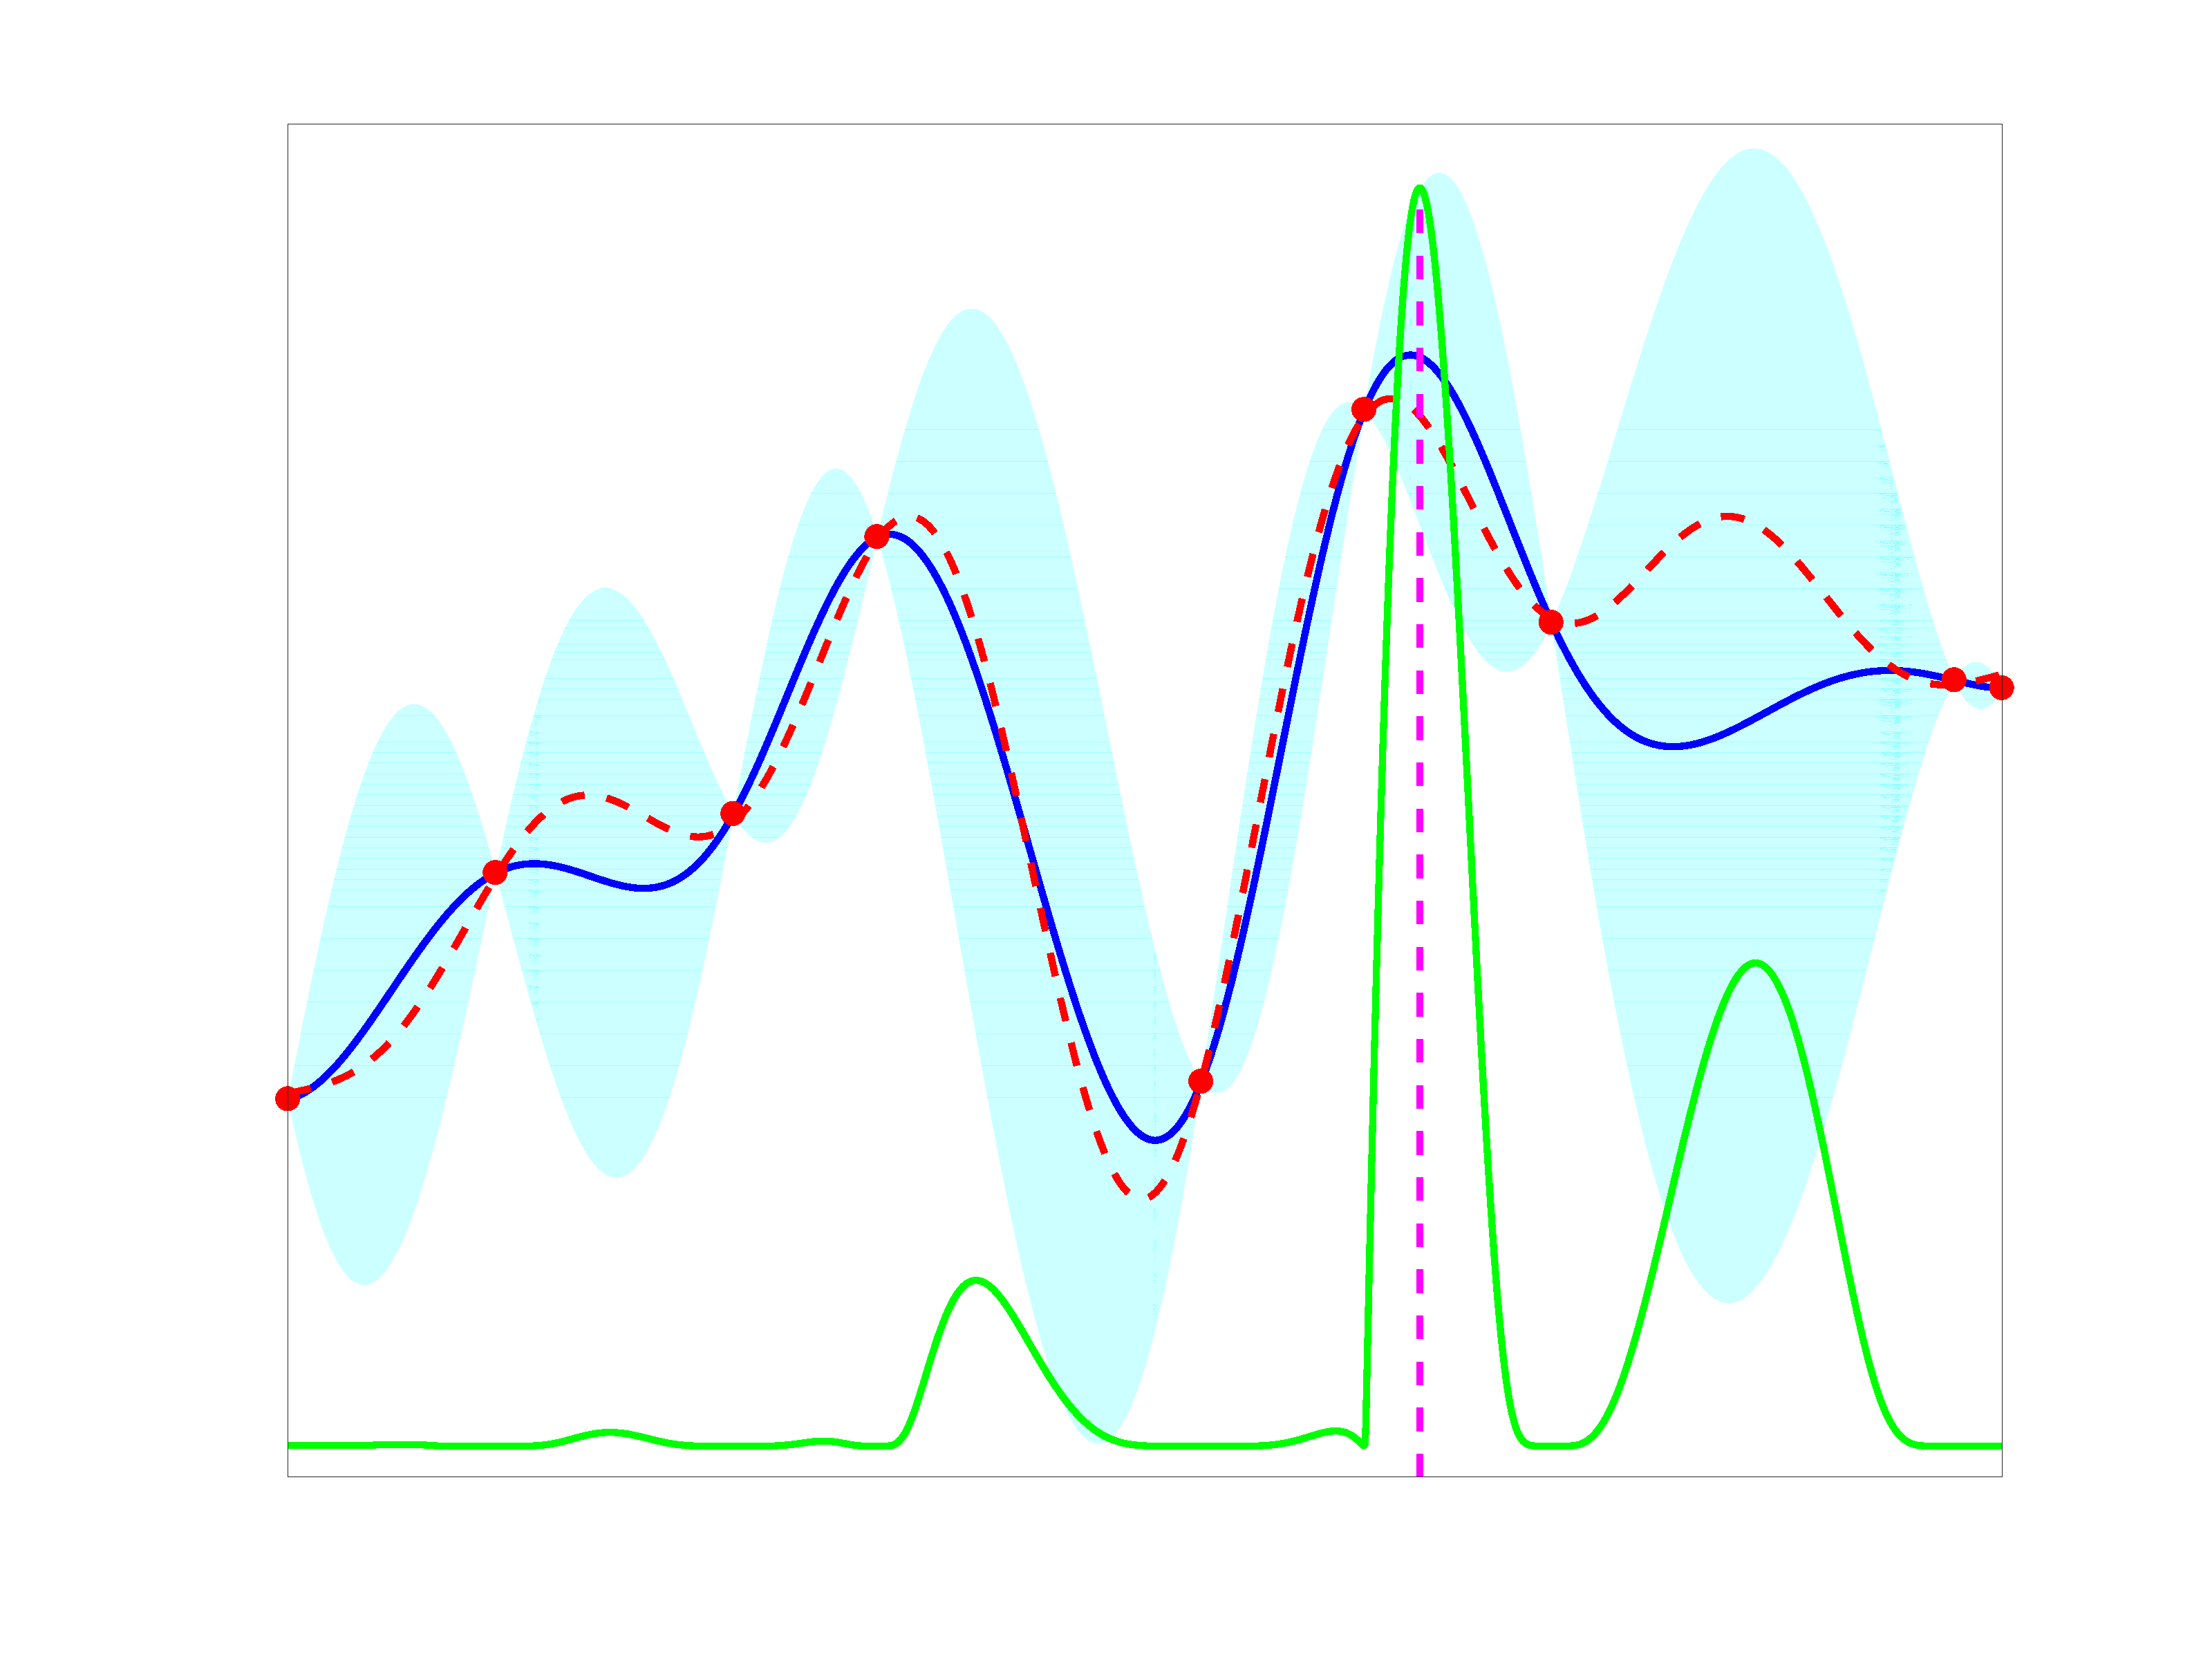
\includegraphics[width=\textwidth,trim={6.8cm 4cm 4.8cm 3cm},clip]{10_with_acq_opt}
		\caption{10 iterations \label{fig:opt:bayes-opt:10}}
	\end{subfigure}
	~
	\begin{subfigure}[b]{0.32\textwidth}
		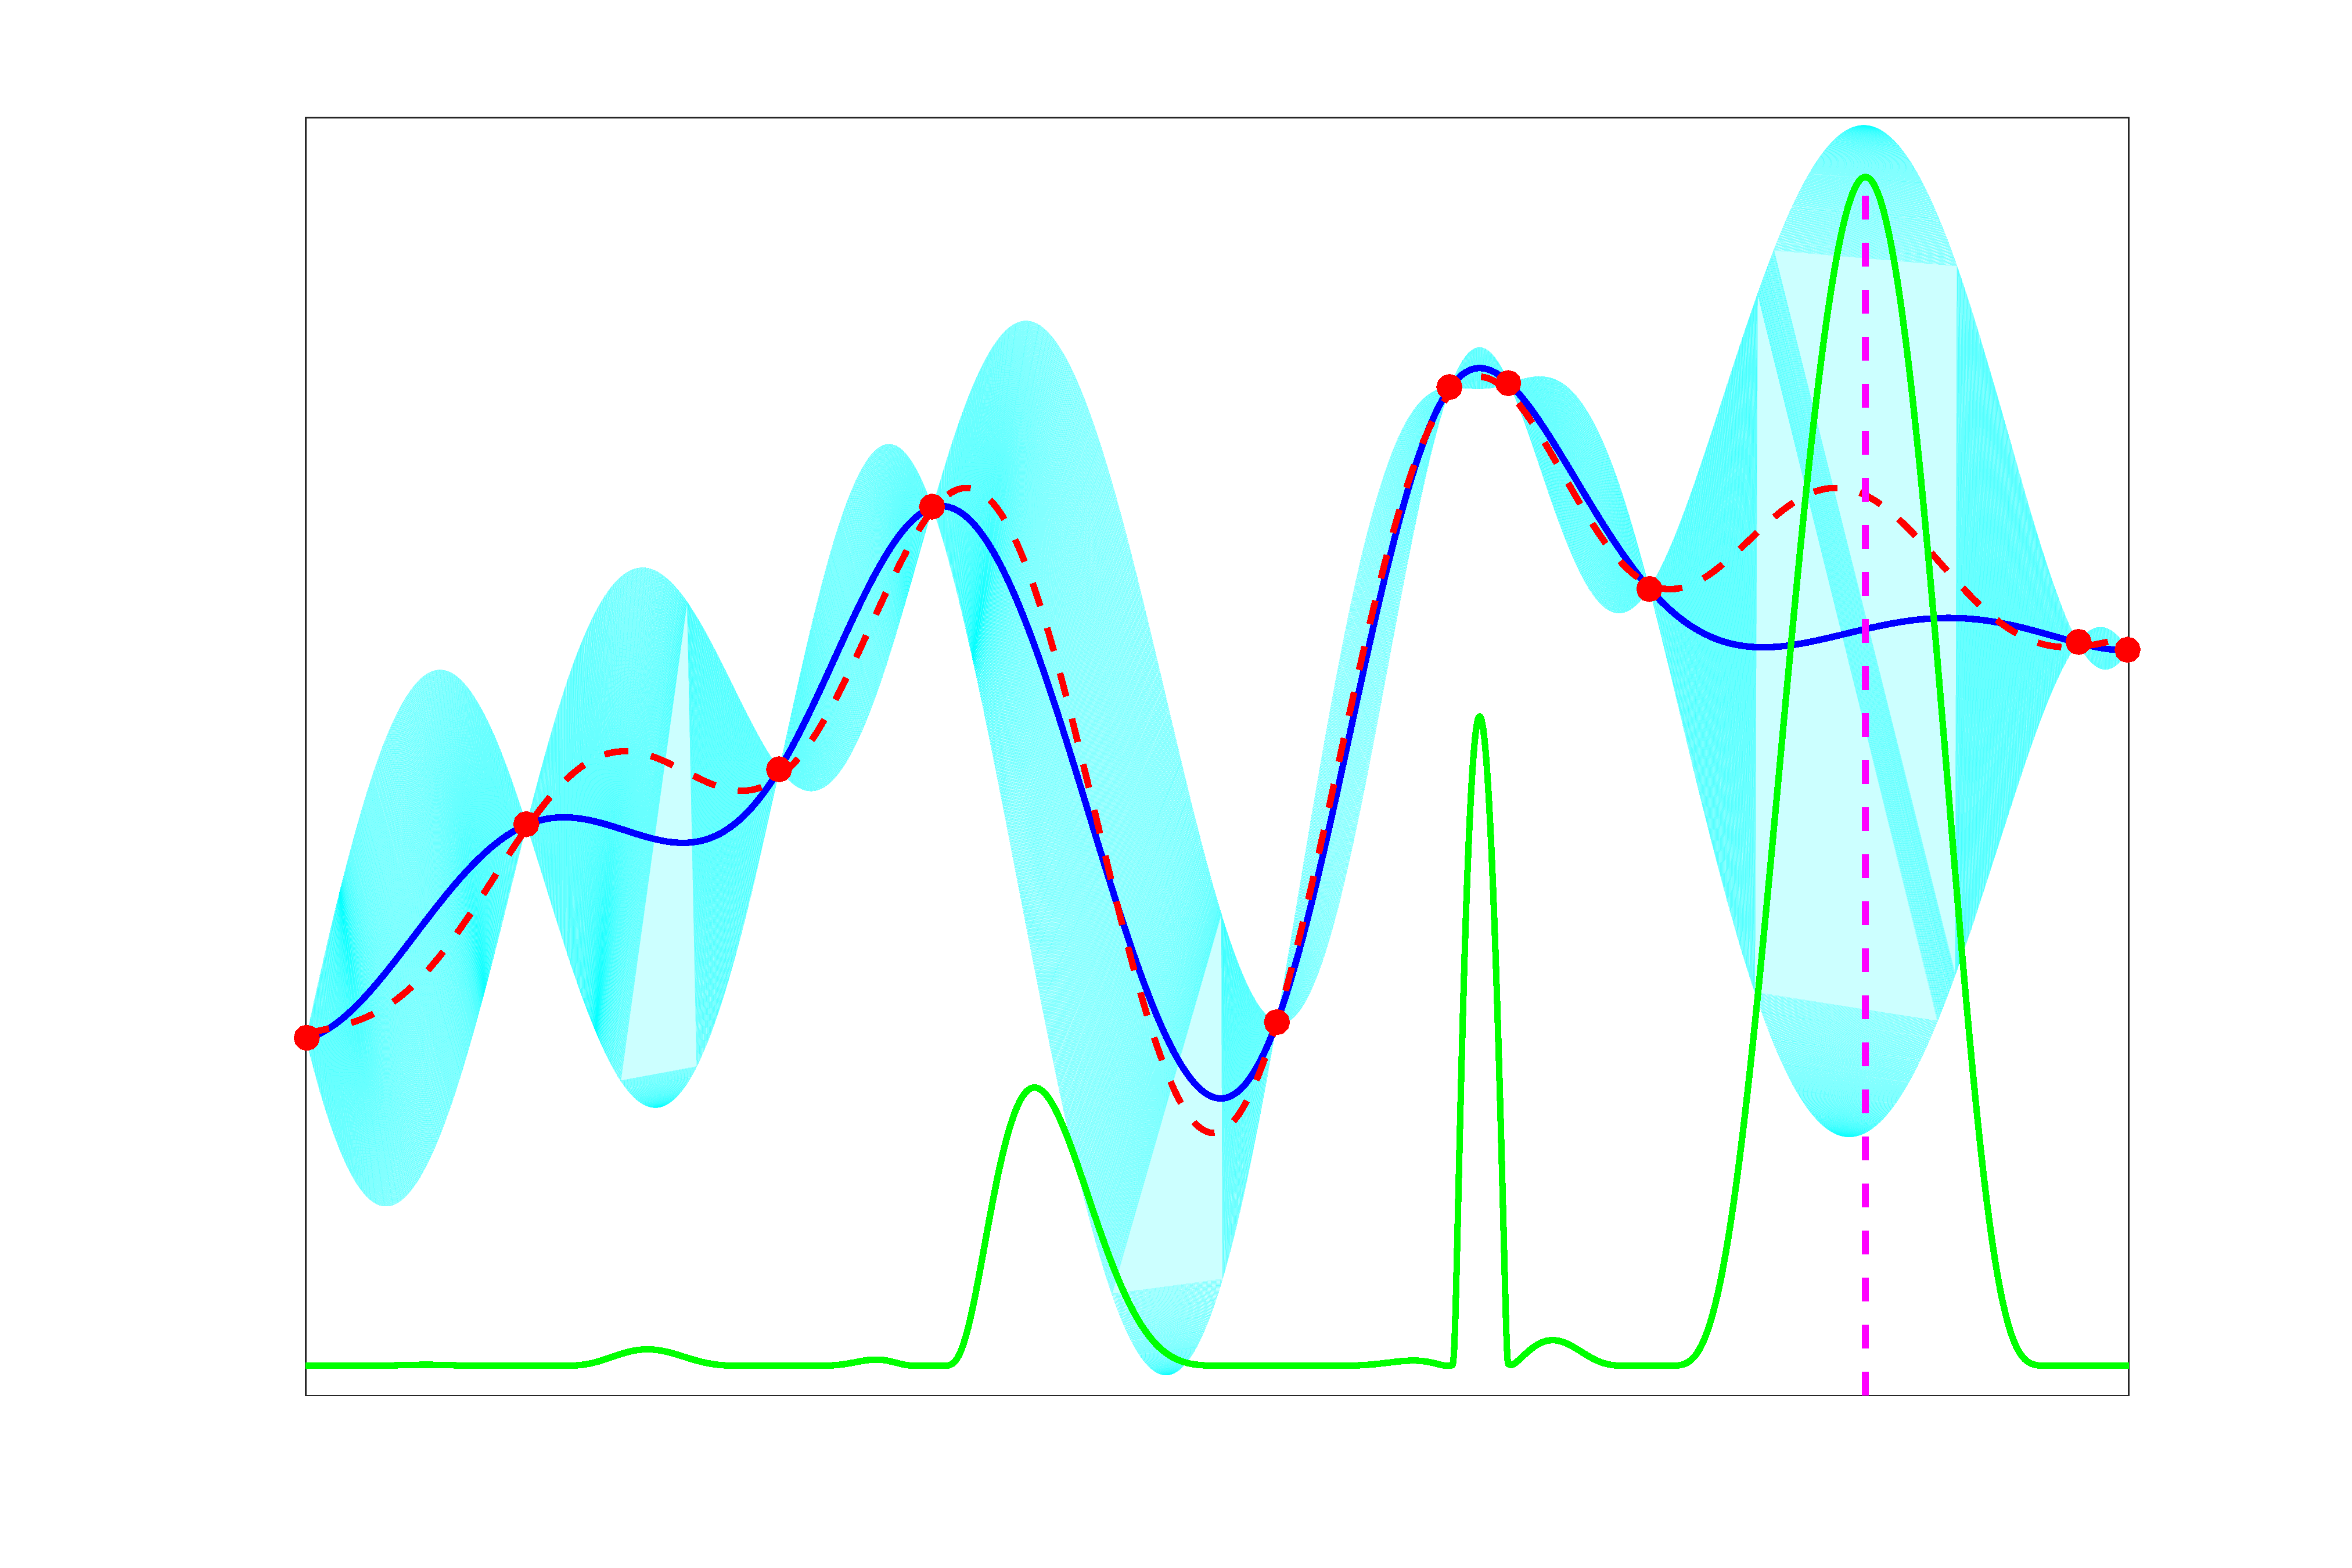
\includegraphics[width=\textwidth,trim={6.8cm 4cm 4.8cm 3cm},clip]{11_with_acq_opt}
		\caption{11 Iterations \label{fig:opt:bayes-opt:11}}
	\end{subfigure}
	~
	\begin{subfigure}[b]{0.32\textwidth}
		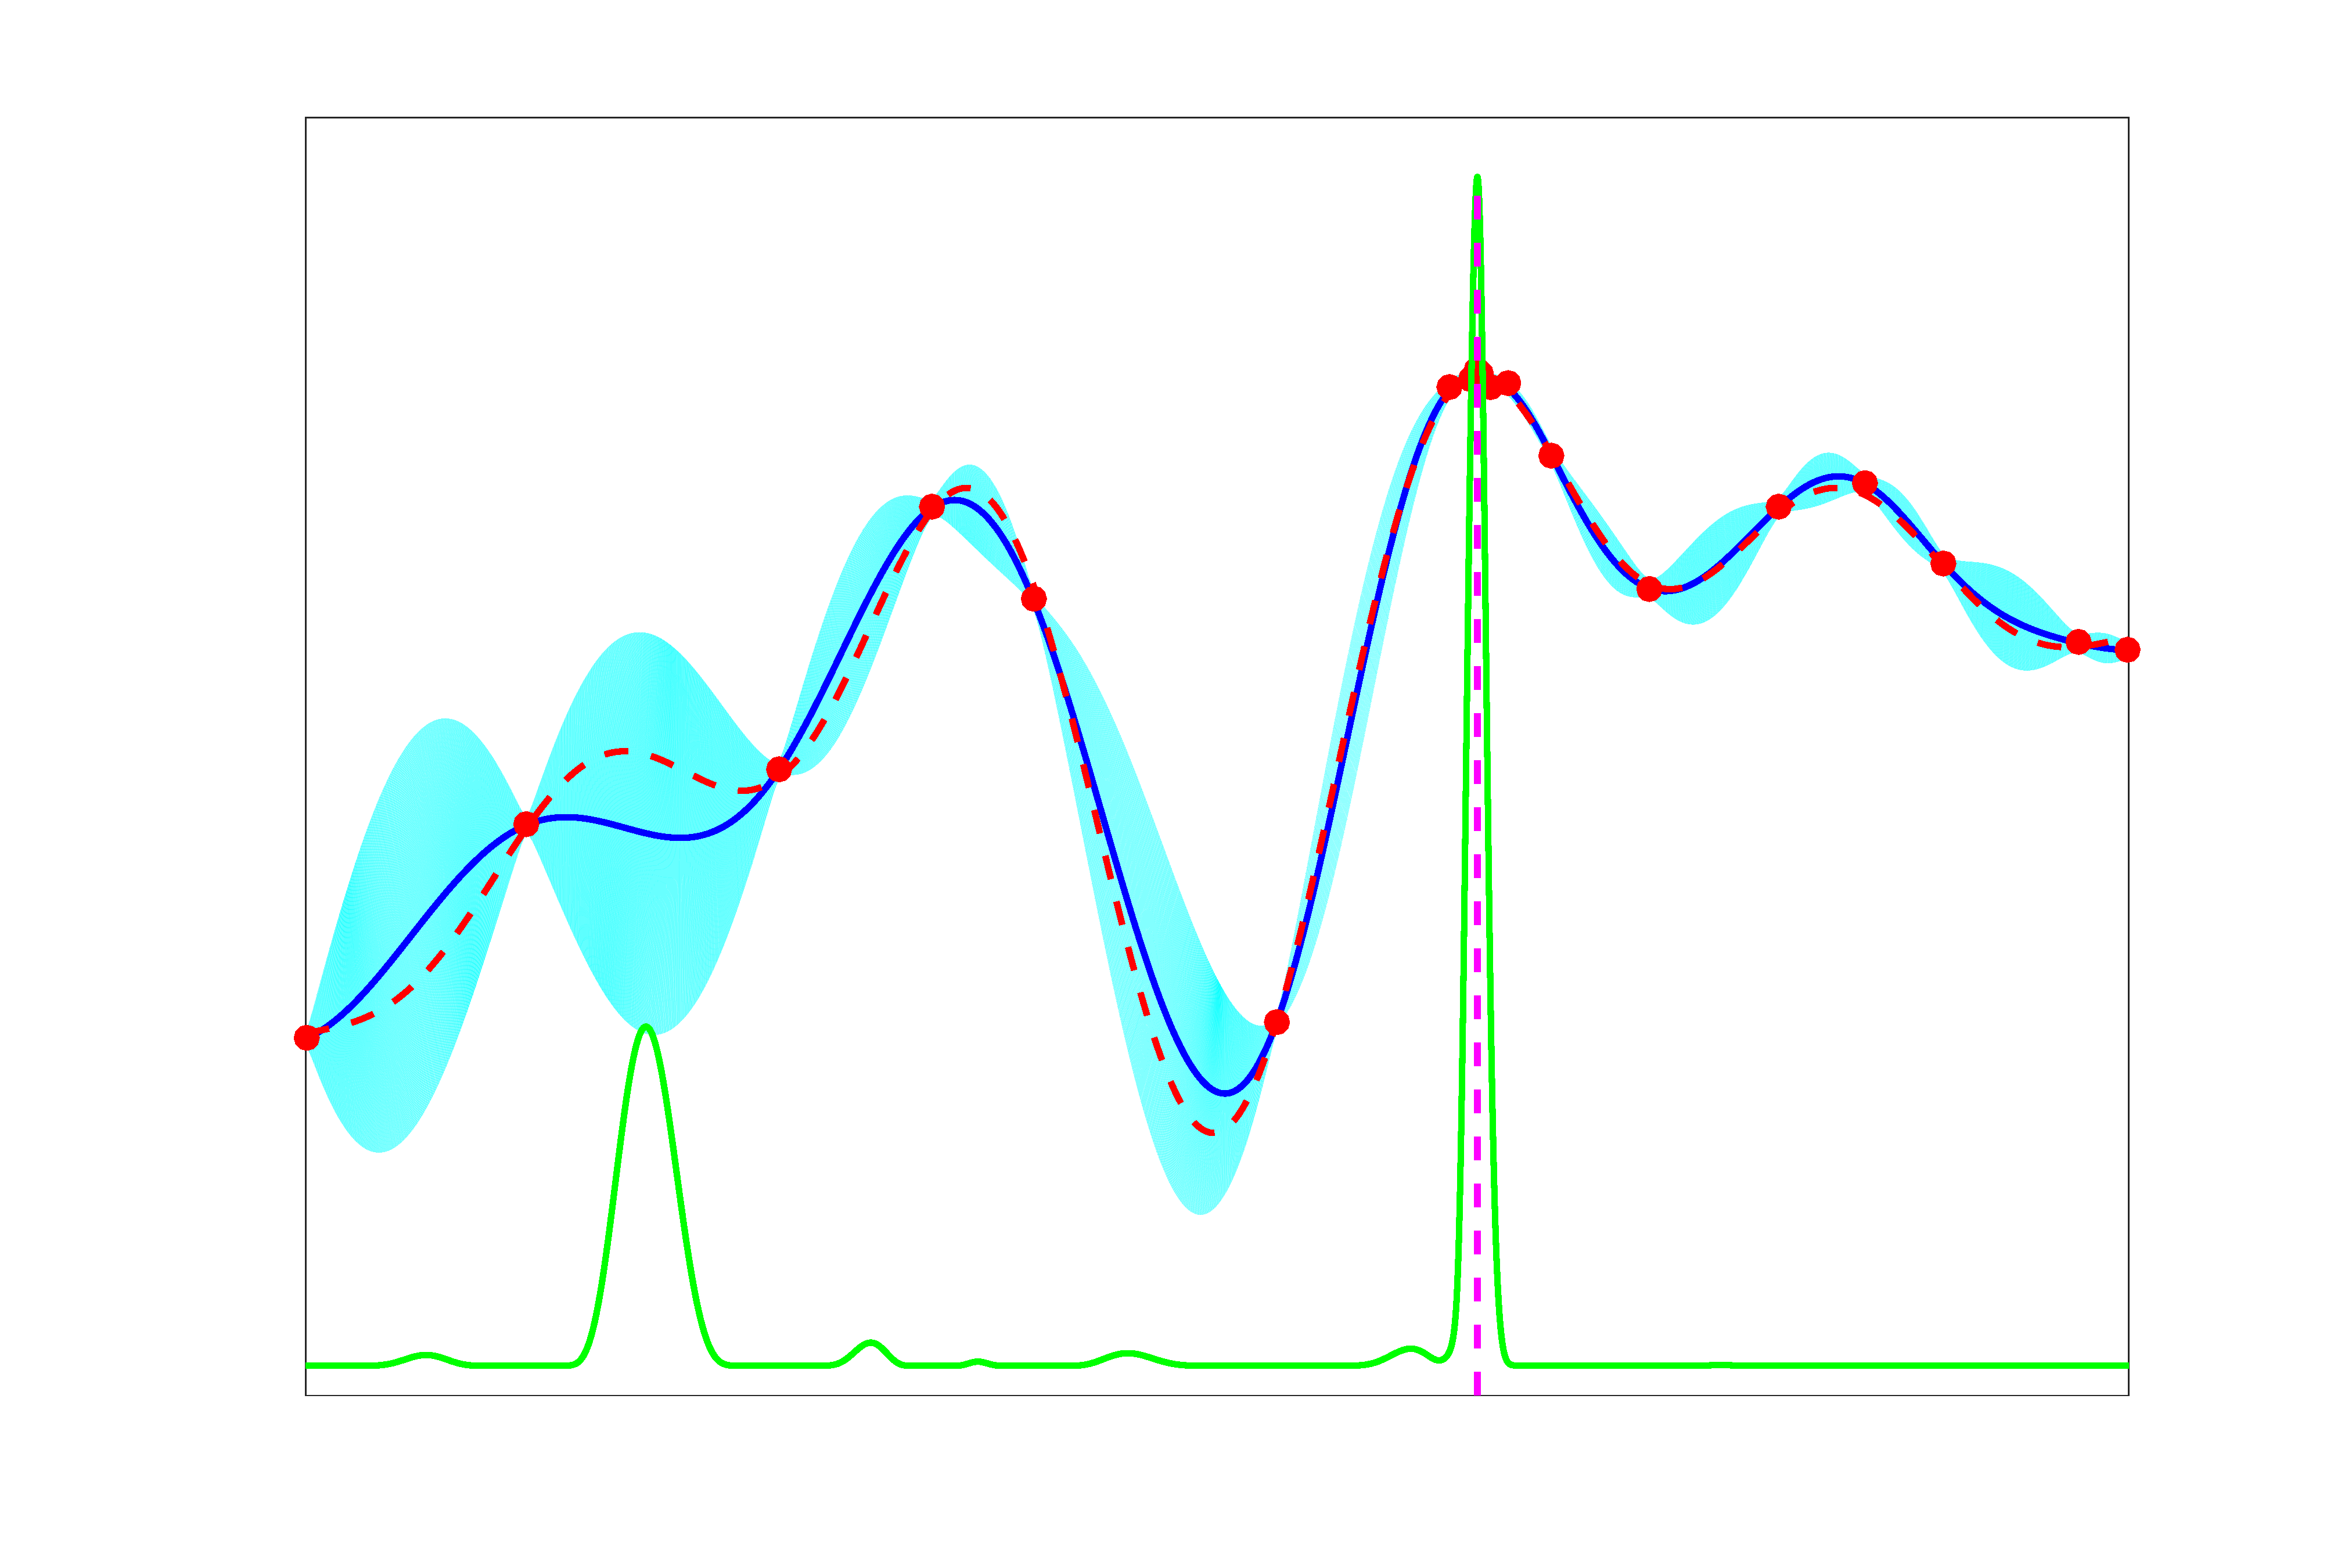
\includegraphics[width=\textwidth,trim={6.8cm 4cm 4.8cm 3cm},clip]{20_with_acq_opt}
		\caption{20 Iterations \label{fig:opt:bayes-opt:20}}
	\end{subfigure}\vspace{5pt}
	%	\begin{tabular}{m{0.15\textwidth} m{0.65\textwidth}}
	%		10 Iterations & 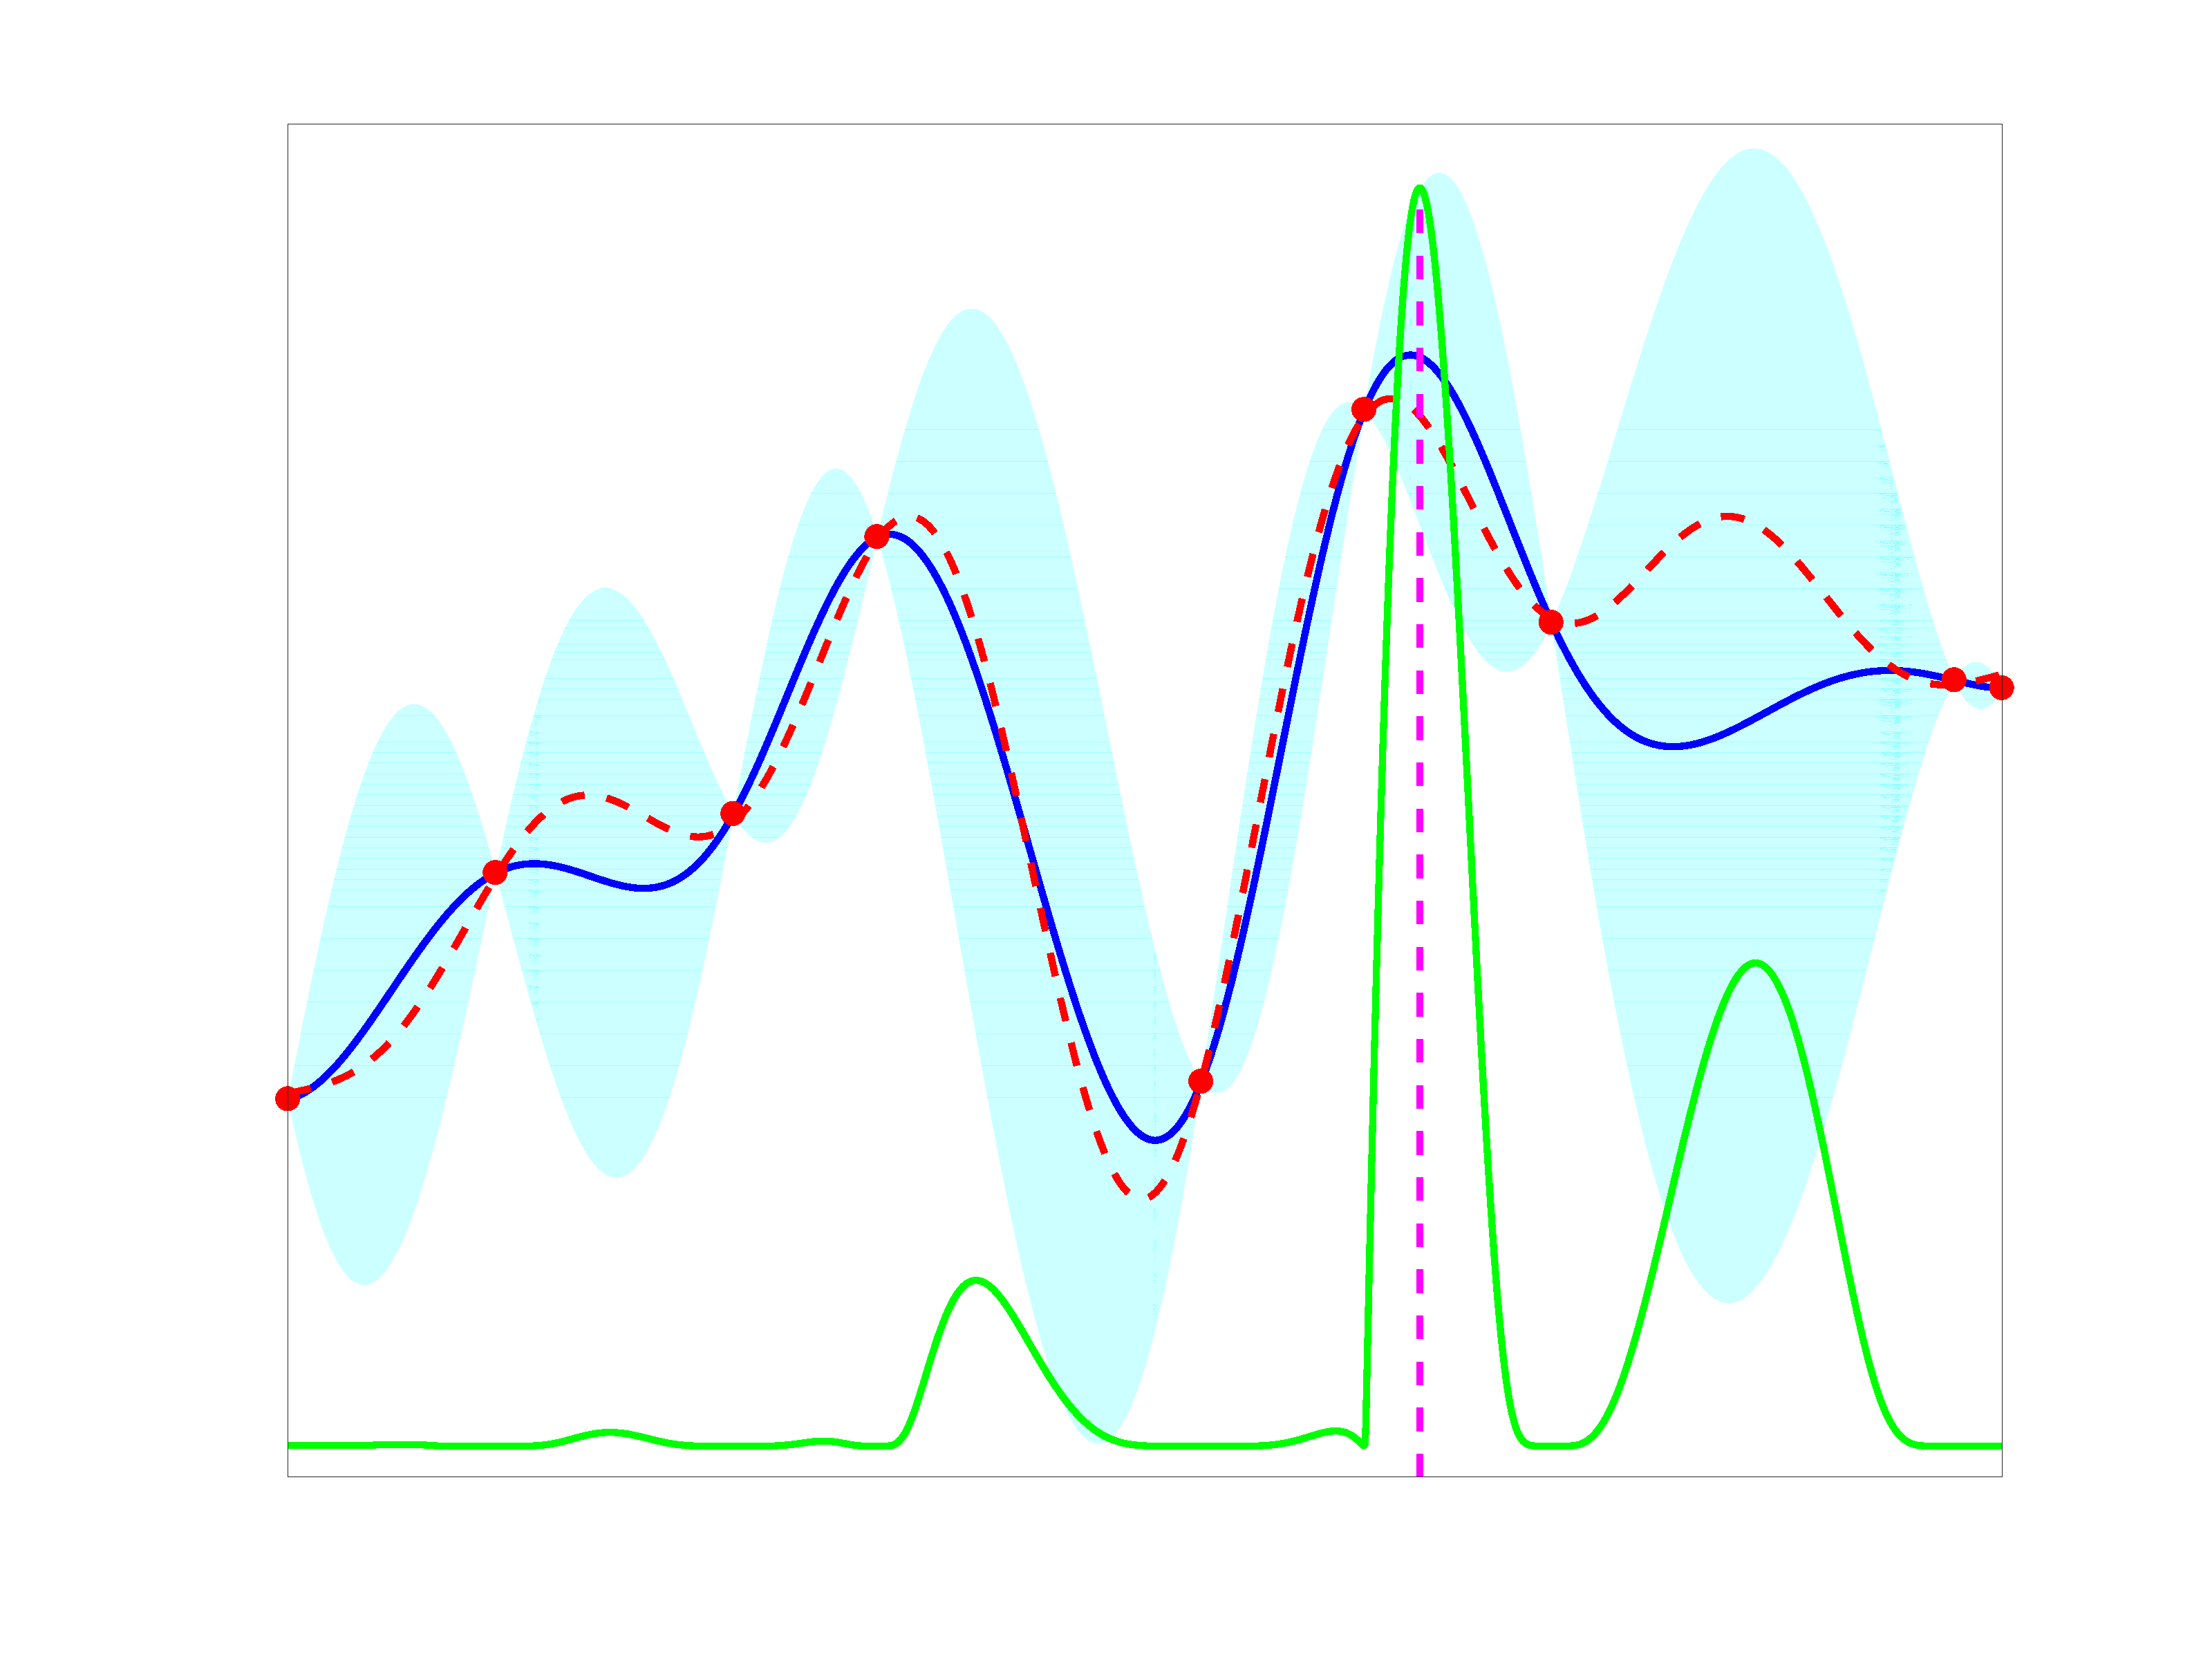
\includegraphics[width=0.6\textwidth]{10_with_acq_opt}
	%		\\
	%		11 Iterations & 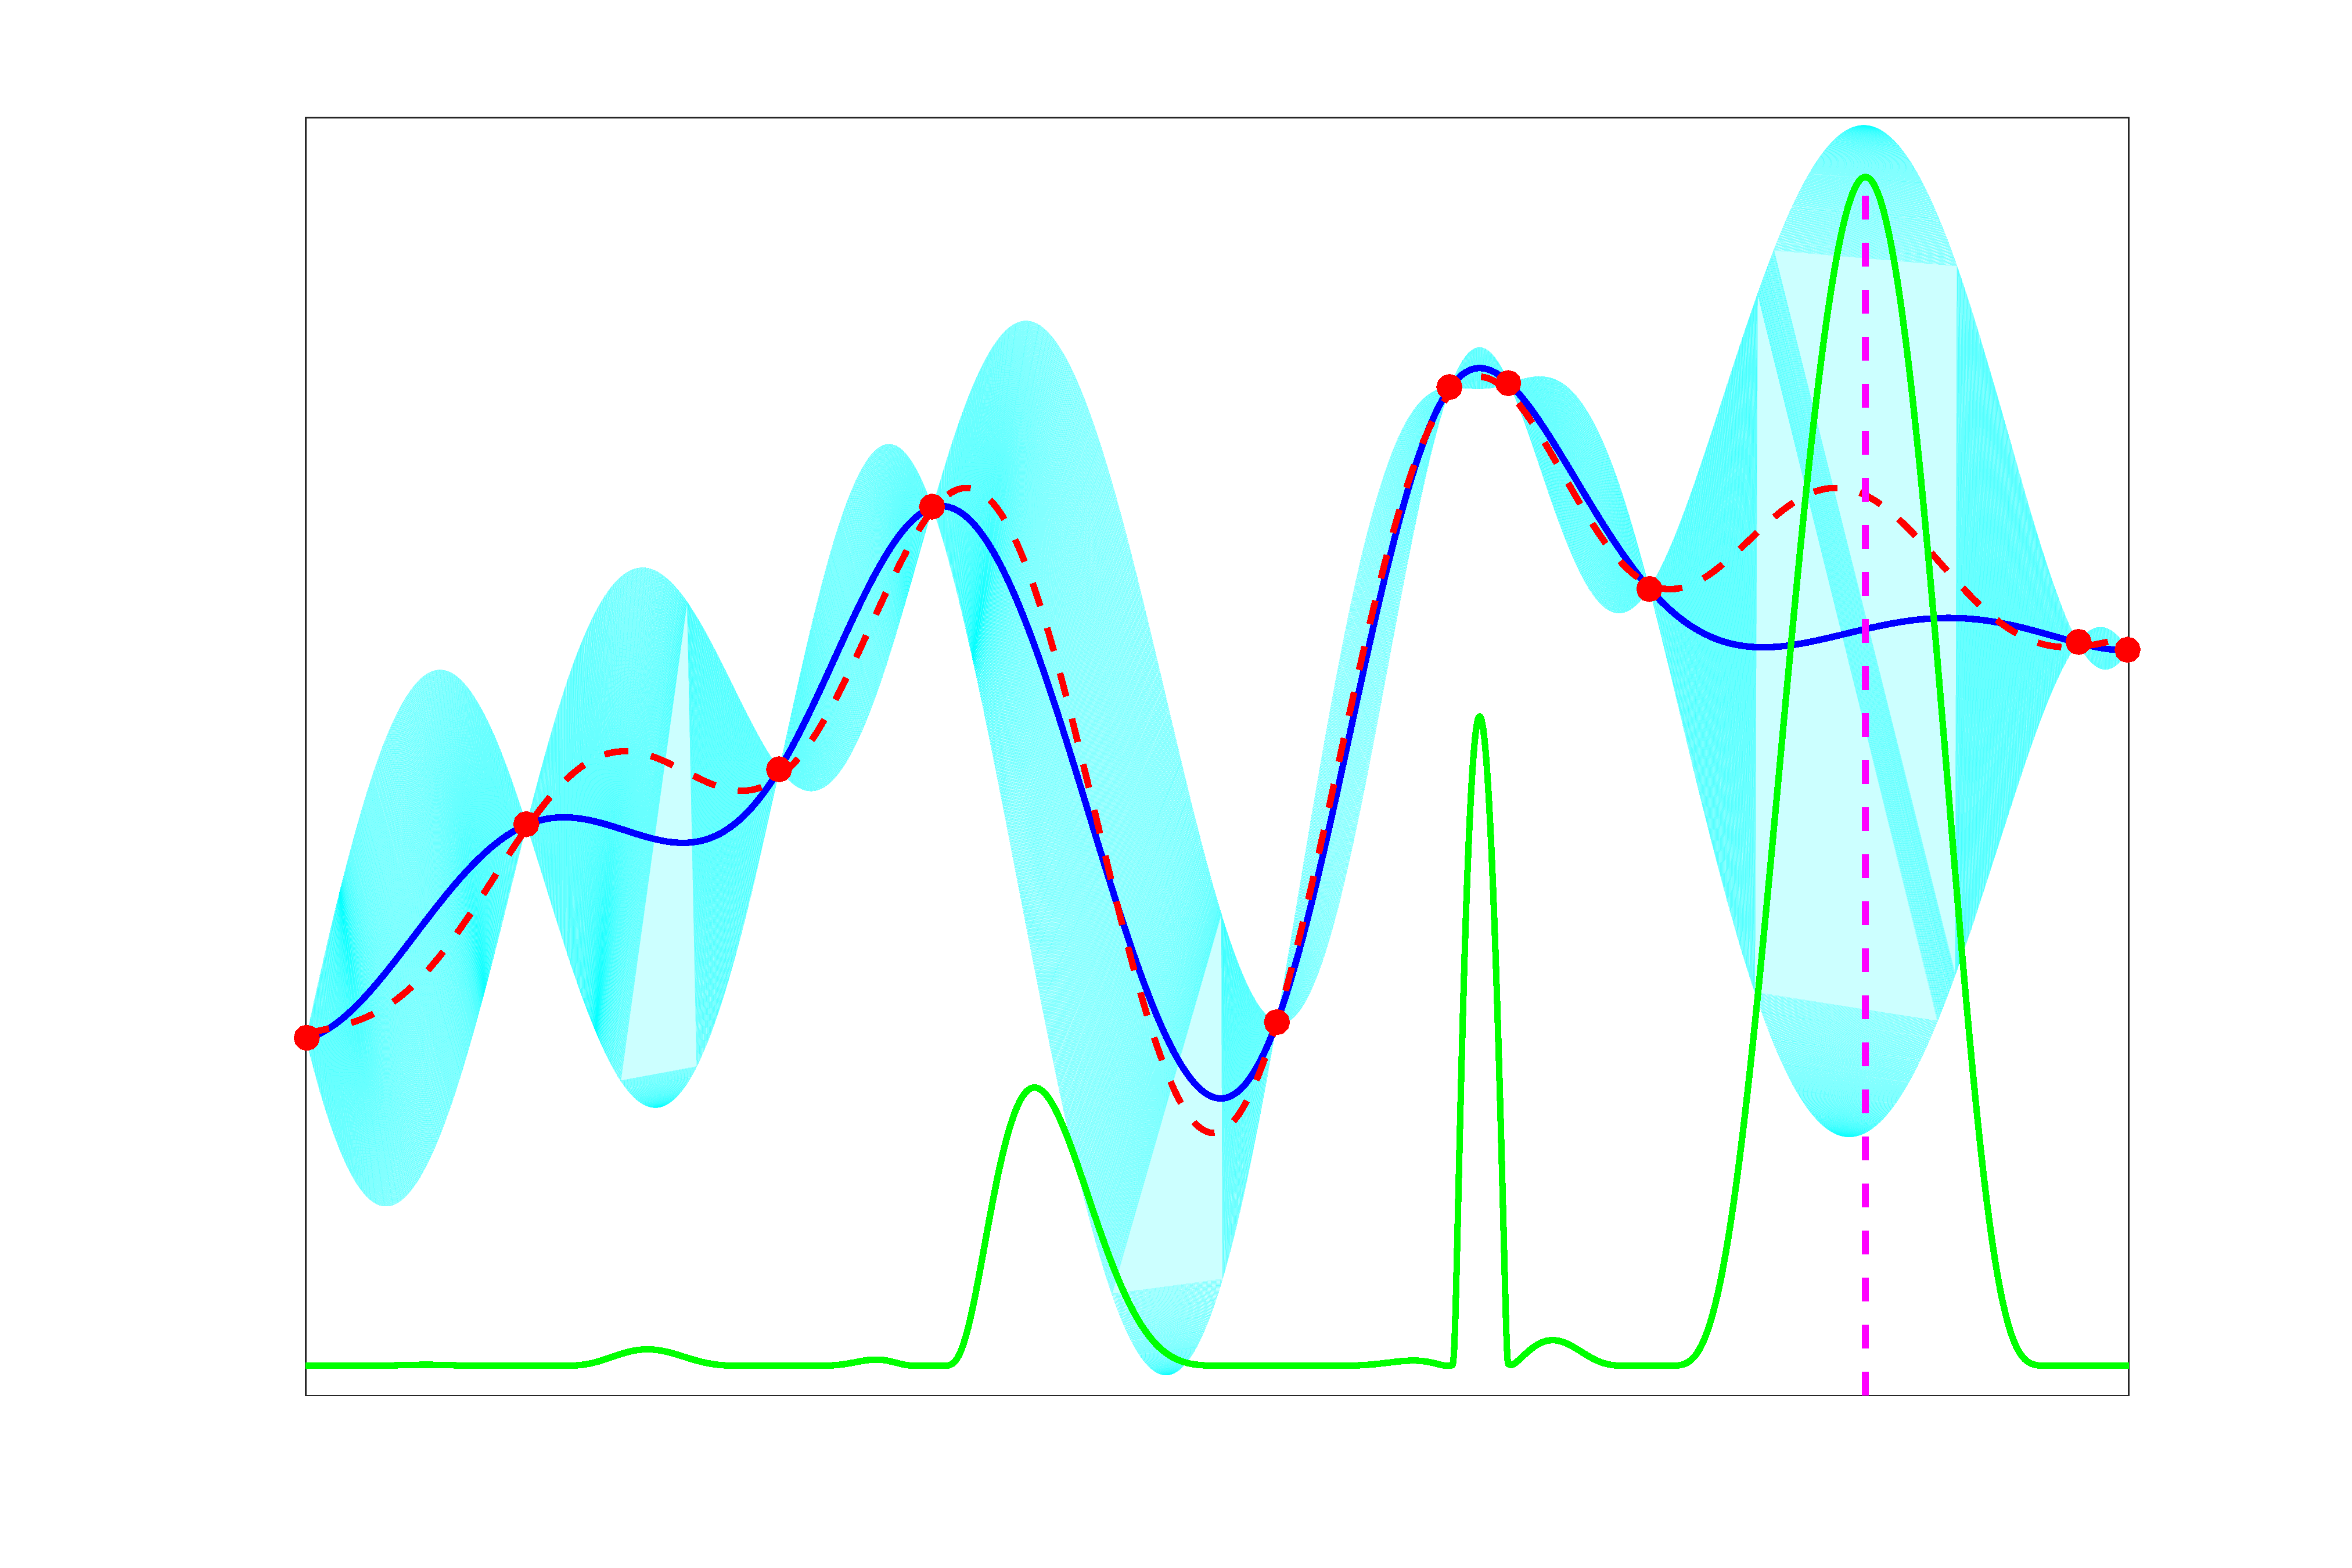
\includegraphics[width=0.6\textwidth]{11_with_acq_opt}
	%		\\
	%		20 iterations & 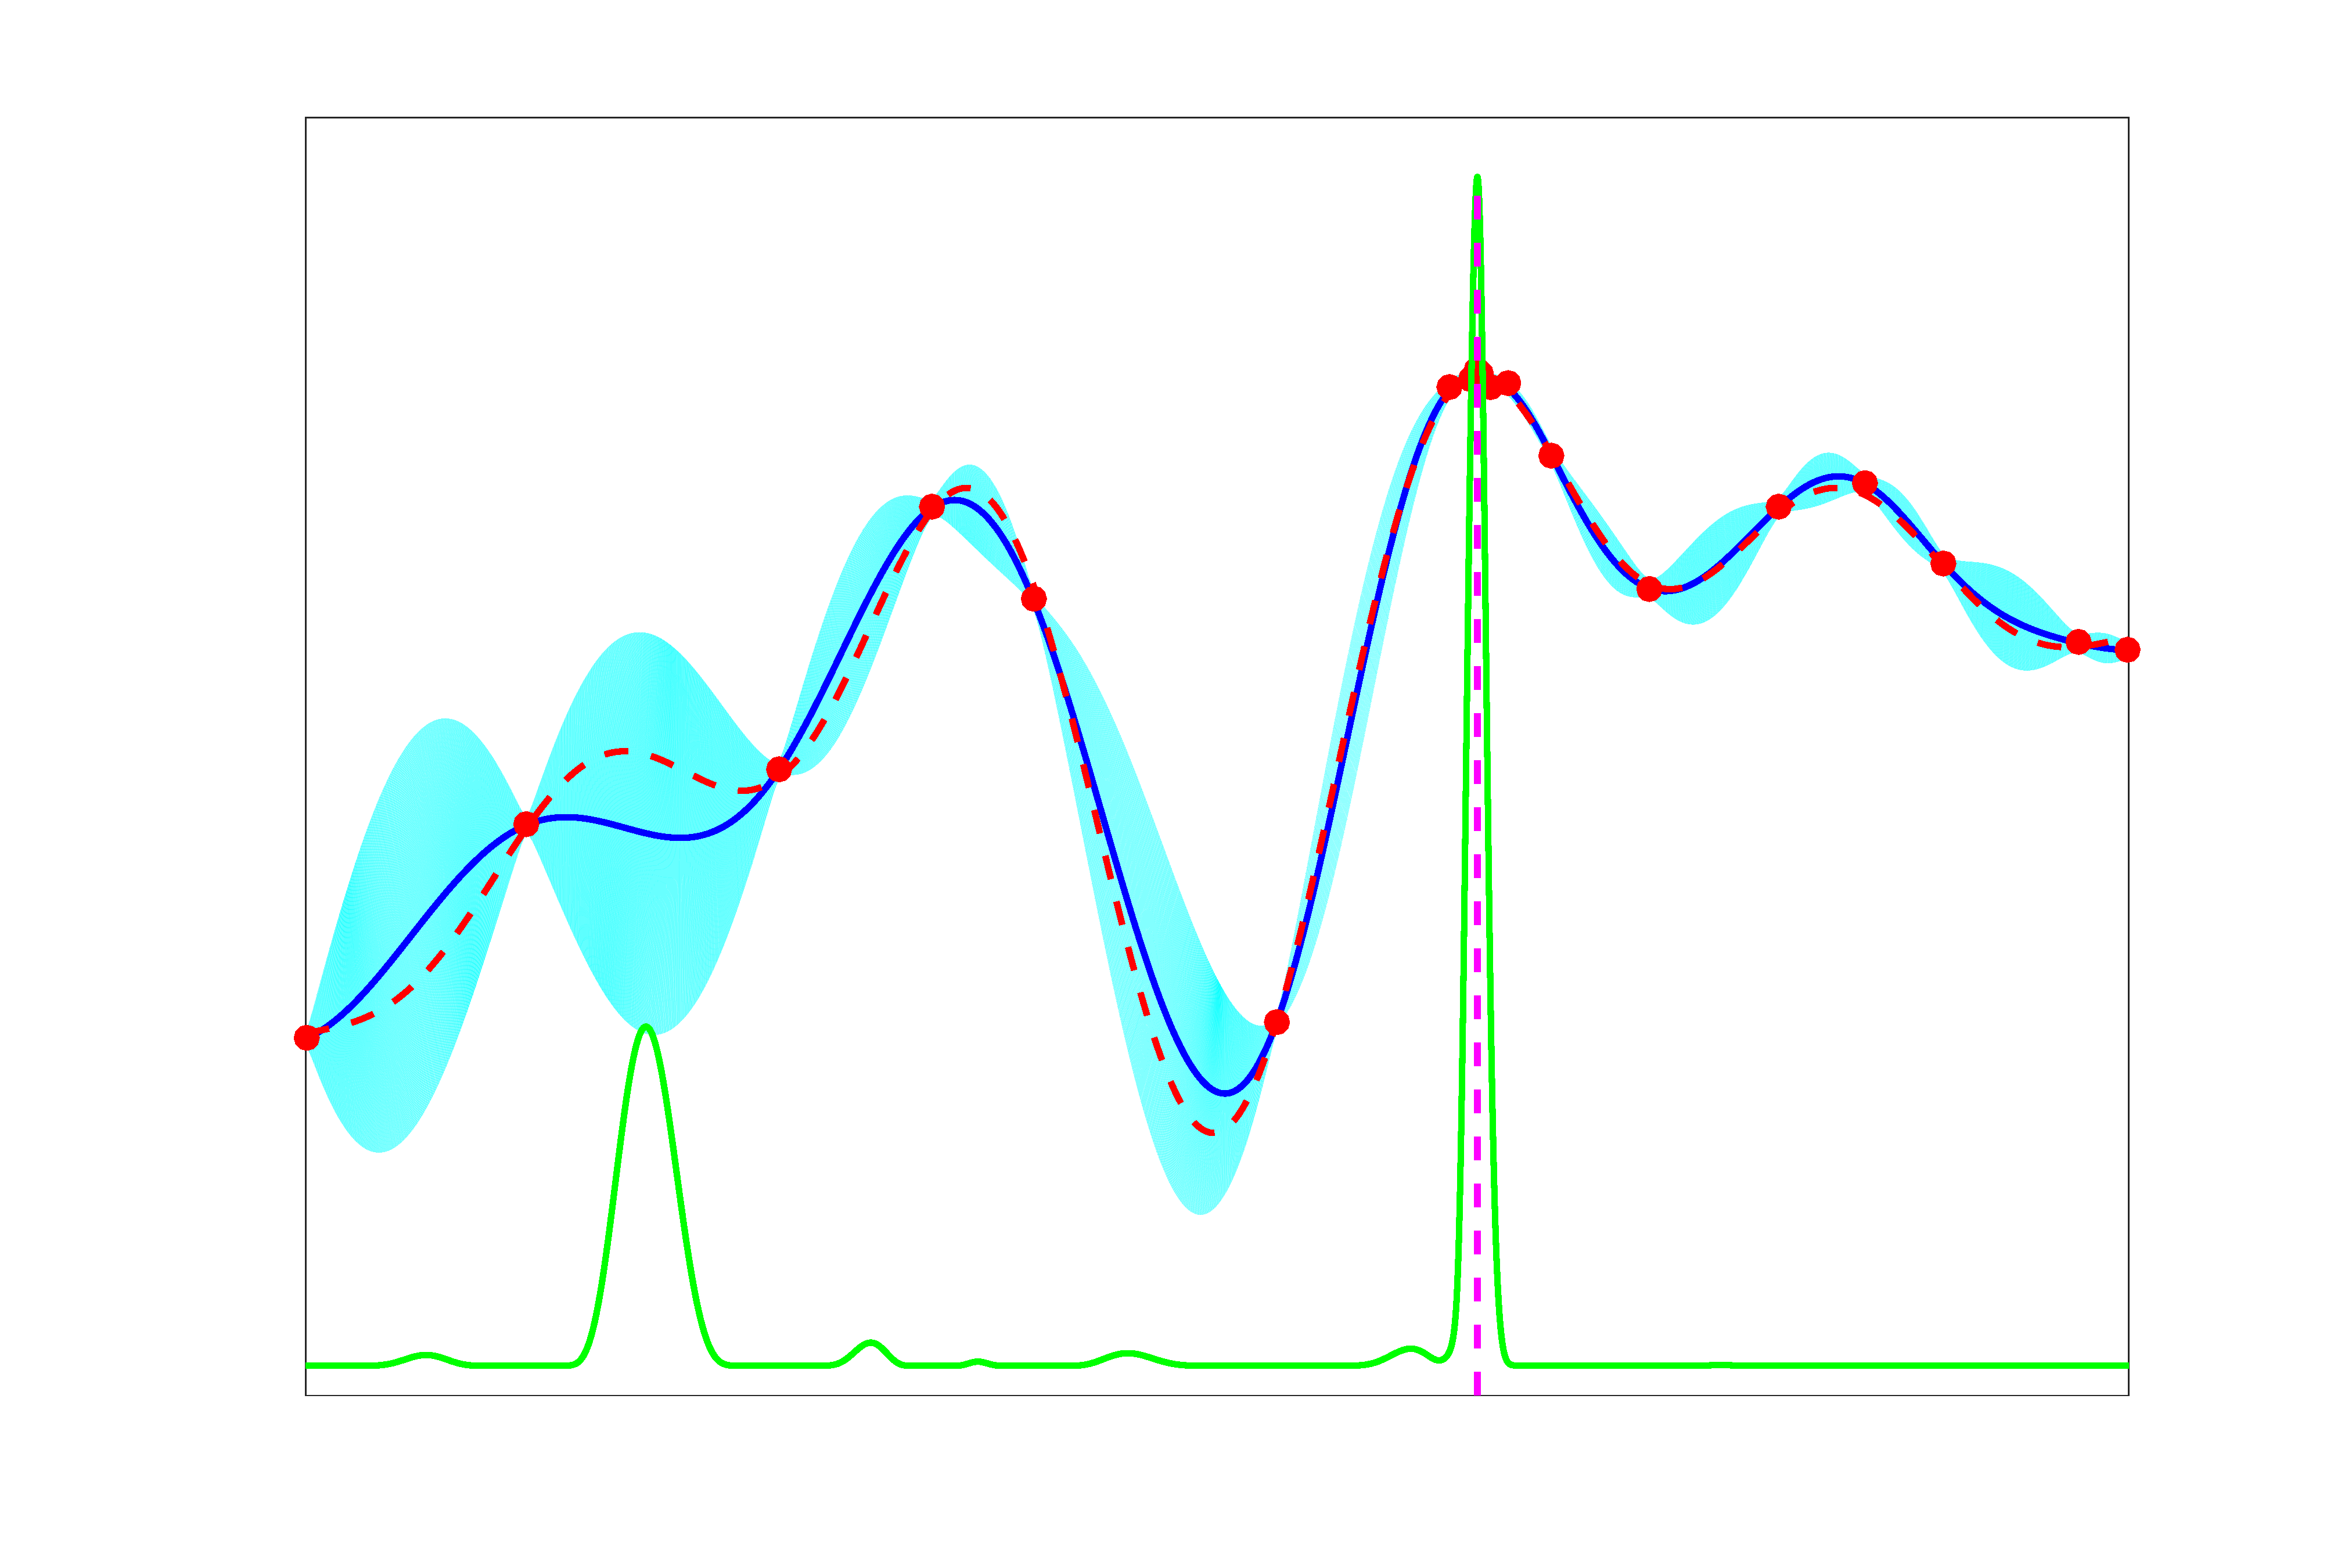
\includegraphics[width=0.6\textwidth]{20_with_acq_opt}
	%	\end{tabular}
	\caption{Illustration of using Bayesian optimization to optimize the
		toy one dimensional problem given in~\eqref{eq:opt:toy}.  Red dots show
		the function evaluations,  the dotted red line shows the true function, 
		the solid blue line is the GP mean, the shaded region is the GP mean $\pm 2$
		standard deviations, the green line is the acquisition function, and
		the dotted purple line is the location of the maximum of the acquisition
		function. See main text for further description.\label{fig:opt:bayes-opt}}
\end{figure}

To solve the first decision -- where to evaluate next -- we specify a so-called 
\emph{acquisition function}  $\zeta : \vartheta \rightarrow \real$
that encodes the relative utility of evaluating a new point.  The optimum of this
acquisition function is then the optimal point to evaluate at the next iteration.
At a high level, the utility
of a point is based on a trade off between \emph{exploration},
namely the desire to evaluate points where our uncertainty is high to reduce the
uncertainty in those regions, and \emph{exploitation}, namely the desire to evaluate points
where the expected function value is high so that we get a good characterization
of the function in promising regions.  One could alternatively think about this as wanting to refine 
the estimates of promising local optima and sample in places that are likely to contain a
missing mode.
We will return to discuss specific acquisition
functions in depth in the next section and for now we simply note that the most
desirable points to evaluate will be those that provide both exploration and exploitation.
For example, consider the expected improvement acquisition function (see~\eqref{eq:opt:EI})
after 10 iterations shown in green in Figure~\ref{fig:opt:bayes-opt:10}.  This is reasonably
large in the two regions of highest uncertainty, but it is highest in the region near the 
true global optima where both
the expected value and uncertainty are high.  After 11 iterations on the other hand,
the uncertainty in this region has dropped dramatically and the point with the
highest uncertainty now has the largest value for the acquisition function.  Note that
the scales for the acquisition functions are different for the different iterations and
that the acquisition function typically decreases as more points are observed.

At first it might seem strange to replace our original optimization problem with
another in the form of optimizing the acquisition function to choose the point
to evaluate next.  This new optimization problem is itself a global
optimization of a typically highly multi-modal function and we need to carry it out
at each iteration of the BO algorithm.  Indeed if the target function $f$ is cheap to
evaluate, taking such an approach would be rather foolish.
The key difference
is that the surrogate optimization problem can be solved without the need to evaluate
the original target function.  Therefore, if $f$ is expensive to evaluate, this additional
computation can be justified if it keeps the number of required evaluations of $f$ to
a minimum.  There are also a number of other features that mean the problem of
optimizing the acquisition function is typically much easier than the original target --
it can be evaluated exactly, derivatives are often available, and provided an appropriate kernel
is used then it is guaranteed to be smooth.  It is also not typically necessary to ensure
that the acquisition function is optimized exactly, as evaluating a point that is
sub-optimal under the acquisition function simply means that a point expected to be less
helpful is evaluated at the next iteration.  This can be useful when the time for a BO
iteration is comparable to a function evaluation, as the amount of computational effort
undertaken by the BO can be tuned to the problem at hand.  It is also worth noting that
the computational complexity for optimizing the acquisition function is theoretically less
(in terms of BO iterations) than the GP training ($O(N^2)$ instead of $O(N^3)$), though the two
are still often comparable for the modest number of iterations BO is
generally run for.

Going back to Figure~\ref{fig:opt:bayes-opt}, we see that BO works by interleaving
regressing a GP to the evaluations, optimizing the acquisition function to find the next
point to evaluate, evaluating the target function at that point, and the updating the GP
regression again.  After 20 iterations for our simple problem, the GP regression around
the optimum has become very accurate, while it is less accurate elsewhere.  This
highlights the sample efficiency of BO as it shows how computational resources are
focussed on where they are required.

Though we have thus far assumed that a GP is used for the surrogate, this is far from the only possible choice
and one can, for example, use random forests \citep{bergstra2011algorithms,hutter2011sequential} 
or neural networks \citep{snoek2015scalable}.  There are a number
of characteristics that make GPs suitable for the surrogate model.  For example, they are very powerful
regressors that can accurately represent the function from relatively few evaluations, especially
for low-dimensional smooth functions.  They also naturally produce uncertainty estimates
that are typically more accurate that those produced by alternatives which often
have to resort to post-processing or heuristics to estimate uncertainty.
This also leads to simple and tractable acquisition functions.  Similarly, their ability to incorporate
noisy observations is often helpful, though because GP inference is only analytic for Gaussian
likelihoods, it is often impractical to incorporate non-Gaussian noise.  This problem can be
particularly manifest when the observations are bounded, such as when the target is a probability
and thus always positive.  A common way of dealing with this is to optimize a mapping of the
original function, for example optimizing the log probability in (M)MAP problems~\citep{osborne2010bayesian}.

When prior information is known about the function, the
flexibility in choosing the covariance kernel can also be very helpful, for example allowing known
smoothness to be incorporated.  However, this can also be a curse as an inappropriate choice of
kernel can severely hamper the performance.  In particular, it will typically be necessary to
do inference over, or at least optimize, the GP hyperparamters.  Another drawback to using GPs
is poor scaling in the number of iterations -- training is a $O(N^3)$ operation due to the required
matrix inversion.  This typically restricts BO using GPs to using on the order of hundreds of iterations
unless appropriate approximations are made~\citep{snelson2006sparse,hensman2013gaussian}.
Another drawback can be poor scaling in the dimensionality of the inputs -- most common kernels
only encode information about the inputs through the (scaled) Euclidean distances between points,
which can break down in high dimensions because all points are typically
``far away'' from one another \citep{bengio2006curse}.  

\subsection{Acquisition Functions}
\label{sec:opt:BO:acq}

As we previously explained, the GP posterior provides convenient analytic representations
for the expected value and uncertainty in the function in the form of the GP posterior mean 
$\mu (\theta)$ and marginal standard deviation $\sigma (\theta)$ respectively.  We now
introduce a number of common acquisition functions, many, but not all, of which will use
these representations directly.
The choice of acquisition function can be critical to the performance of Bayesian optimization
and its choice forms a basis for a significant proportion of the Bayesian optimization
literature~\citep{shahriari2016taking}.  In particular, some acquisition functions have
pathologies, for example probability of improvement has a tendency to insufficiently explore, which can severely impede the
performance of BO.  This has lead to the development of some very powerful, but computationally
intensive and algorithmically complicated, acquisition strategies (e.g.~\cite{hernandez2014predictive}), 
such that there is often a speed / simplicity vs per iteration performance trade-off in their selection.

%\begin{figure}[t]
%	\centering
%	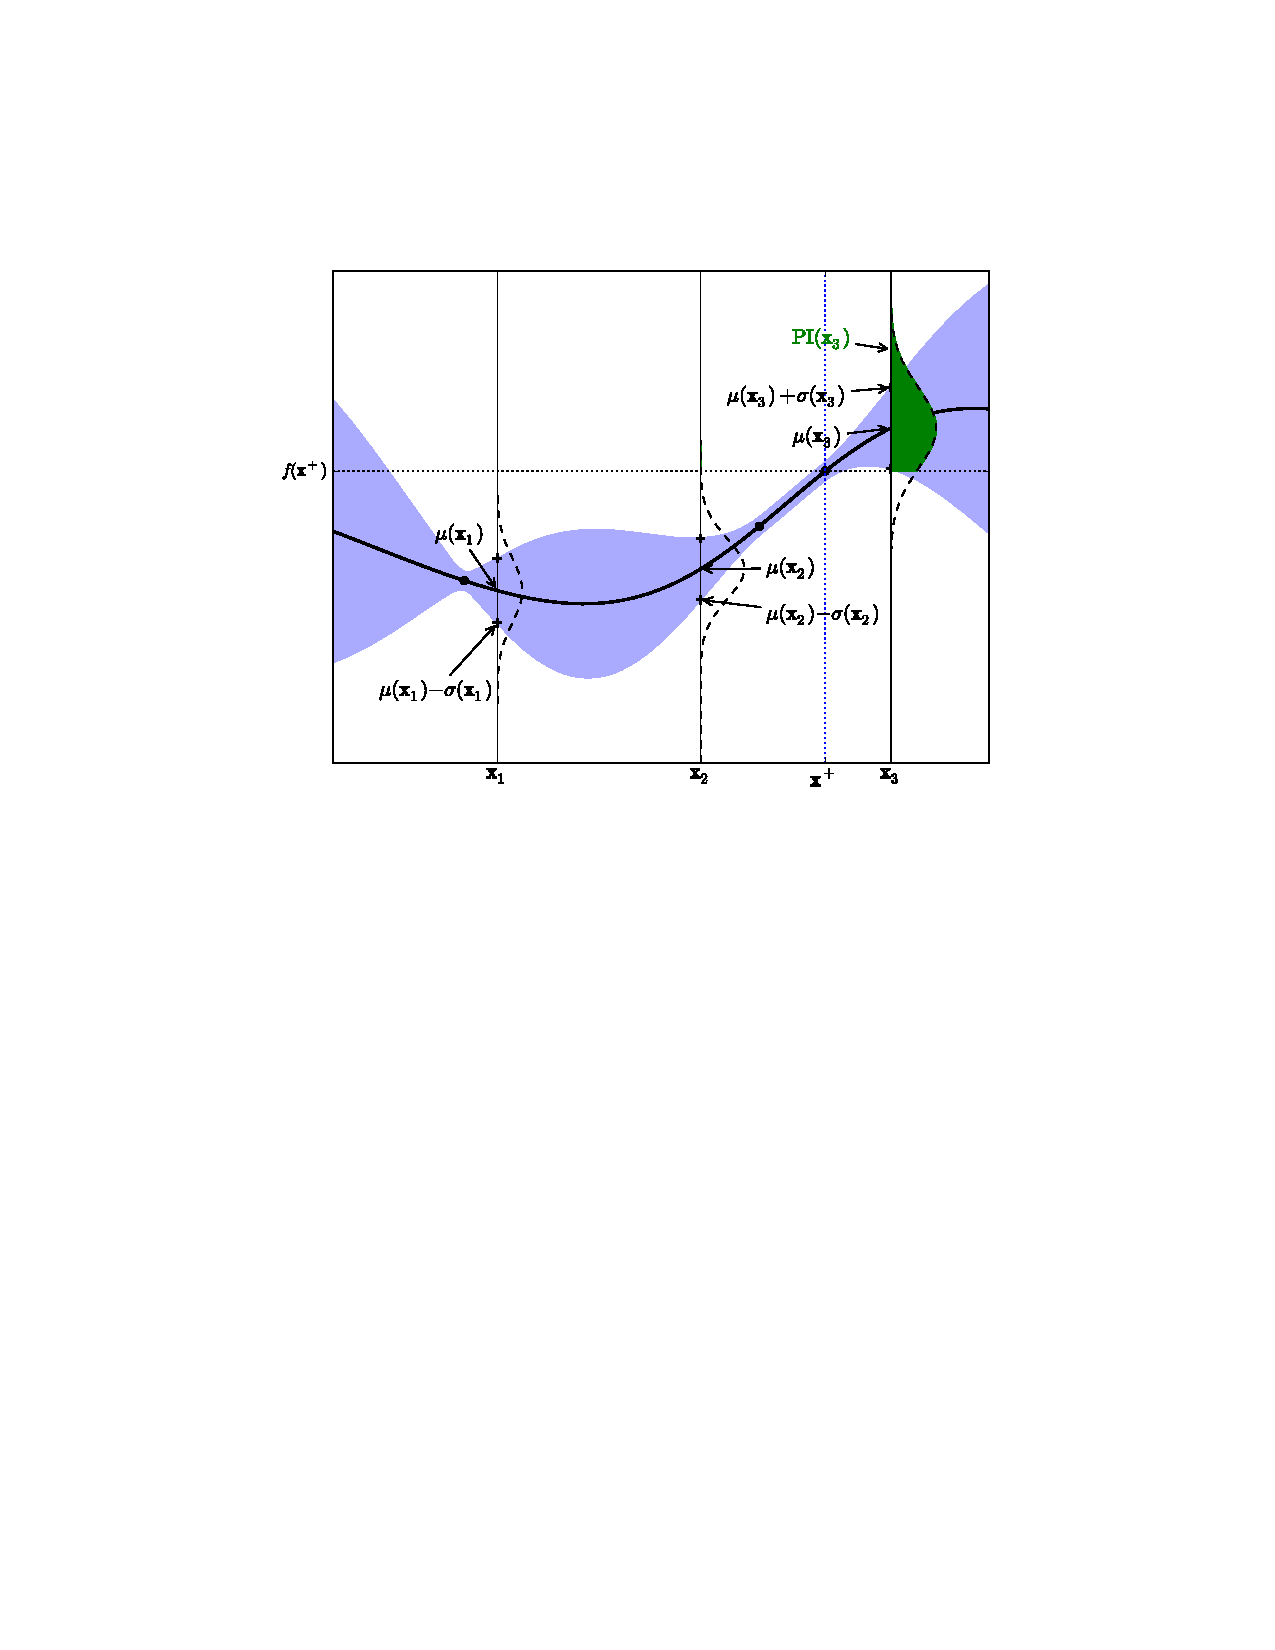
\includegraphics[width=0.95\textwidth]{prob_imp_brochu}
%	\caption{Explanation figure for probability of improvement, taken from~\cite{brochu2010tutorial}.
%		The best point so far (i.e. evaluated point with the highest GP mean) occurs at $\mathbf{x}^+$,
%		with corresponding GP mean $\mu(\mathbf{x}^+)$ (for some reason $f(\mathbf{x}^+)$ is shown
%		instead).  The probability of improvement at any point corresponds to the marginal probability that the 
%		the true function value at that point is larger than $\mu(\mathbf{x}^+)$.  An example of which is 
%		shown at the point $\mathbf{x}_3$, corresponding to the green shaded region, which is clearly
%		substantially larger than at two other hypothetical points $\mathbf{x}_1$ and $\mathbf{x}_2$.
%		Note also that the expected improvement of $\mathbf{x}_3$ corresponds to the expectation 
%		of $\mathbf{x}_3-\mathbf{x}^+$ under the distribution of the green shaded region, while the 
%		point $\mu(\mathbf{x}_3)+\sigma(\mathbf{x}_3)$ corresponds to the UCB acquisition function
%		with $\kappa=1$.
%		REPLACE WITH OWN FIGURE\label{fig:opt:prob-imp}}
%\end{figure}

\subsubsection{Probability of Improvement}
\label{sec:opt:BO:acq:prob}

One of the conceptually simplest acquisition functions is the probability of improvement (PI, \cite{kushner1964new}), namely
the probability that the function value at a point is higher than the current estimated optimum.
 As shown by, for example,
\cite{brochu2010tutorial}, the probability of improvement has a simple analytic form because the
marginal distributions for function evaluations are Gaussian.  Specifically, let
\begin{align}
\label{eq:opt:muplus}
\mu^+ = \max_{j\in \{1,\dots,m\}} \mu\left(\theta_j\right)
\end{align}
denote the point with the highest expected value and define
\begin{align}
\label{eq:opt:gamDef}
\gamma\left(\theta\right) = \frac{\mu \left(\theta\right)-\mu^+-\xi}{\sigma\left(\theta\right)},
\end{align}
where $\xi \ge 0$ is a user set parameter.
The probability of improvement is then defined as the probability of improving the 
objective function by at least an amount $\xi$
\begin{align}
\label{eq:opt:PI}
\mathrm{PI}\left(\theta\right) = p \left(f\left(\theta\right)\ge \mu^+ +\xi\right) = \Phi \left(\gamma\left(\theta\right)\right)
\end{align}
where $\Phi \left(\cdot\right)$ represents the unit normal cumulative distribution function.  
Note that $\xi=0$ corresponds to pure exploitation and $\xi \rightarrow \infty$ 
corresponds to pure exploration.  Typically for PI, one will employ a cooling schedule 
for $\xi$ to incorporate the intuitive idea that one should first explore and then 
exploit.  However, as shown by for example \cite{jones2001taxonomy}, 
the performance of the PI acquisition function is sensitive to the choice of 
$\xi$ and therefore the cooling strategy requires careful tuning.  Doing this effectively in
a general purpose way is very challenging, meaning that PI
is rarely used in practice.

\subsubsection{Expected Improvement}
\label{sec:opt:BO:acq:expt}

A method less sensitive to tuning is the expected improvement~\citep{movckus1975bayesian}.  
It is conceptually similar to PI, but incorporates the idea that large improvements are more beneficial
to small improvements. It therefore better represents the importance of exploration and
is less prone to over-exploitation.
It can also be calculated analytically for a GP (see e.g. \cite{brochu2010tutorial}) leading to
the following definition
\begin{align}
\label{eq:opt:EI}
\begin{split}
\mathrm{EI} \left(\theta\right) = & \int_{\mu^+ +\xi}^{\infty} p\left(f\left(\theta\right)|\mu\left(\theta\right),\sigma\left(\theta\right)\right) \left(f\left(\theta\right)-\mu^+-\xi\right) df\left(\theta\right) \\
= & \begin{cases}
\left(\mu\left(\theta\right)-\mu^+-\xi\right)\Phi \left(\gamma\left(\theta\right)\right)+\sigma\left(\theta\right)\phi\left(\gamma\left(\theta\right)\right), & \sigma \left(\theta\right) > 0 \\
0, & \sigma \left(\theta\right) = 0
\end{cases}
\end{split}
\end{align}
were $\phi \left(\cdot\right)$ represents the probability density function of the unit normal distribution.  
The parameter $\xi$ plays a similar role as for the PI, but in this case $\xi=0$ no longer corresponds 
to pure exploitation.  \cite{lizotte2008practical} suggests that cooling schedules on $\xi$ are 
not helpful for EI and that $\xi = 0.01 \mathbb{E} \left[\sigma \left(\theta\right)\right]$ where 
$\mathbb{E} \left[\sigma \left(\theta\right)\right]$ is signal standard deviation works well in almost all cases.
Simply setting $\xi=0$ is also a common choice, but it can be prone to doing insufficient exploration.
Convergence rates for EI have been demonstrated by~\cite{bull2011convergence}.

\subsubsection{Upper Confidence Bounding}
\label{sec:opt:BO:acq:ucb}

Another possible acquisition strategy is to maximize the upper confidence bound (UCB) for
the function value~\citep{lai1985asymptotically,srinivas2009gaussian}, namely
\begin{align}
\label{eq:UCB}
\mathrm{UCB}\left(\theta\right) = \mu \left(\theta\right) + \kappa \sigma \left(\theta\right)
\end{align}
where $\kappa \ge 0$ is again a parameter that will control the exploration / exploitation trade off.
This bound represents the point at which the probability the function is less than this value is $\Phi (\kappa)$.
A particularly nice feature of the UCB acquisition function is that given certain conditions on 
$\vartheta$ and $k$, $\kappa$ can be chosen in a manner such that acquisition has bounded 
cumulative regret with high probability, this is known as GP-UCB \citep{srinivas2009gaussian}. 
However, the need to (often adaptively) set $\kappa$ can be a noticeable drawback.

\subsubsection{Information-Based Policies}
\label{sec:opt:BO:acq:inf}

At the end of the day, the aim of BO is to find the location of the optimum.  The true utility of
evaluating a new point is, therefore, in the information it provides about the location of the
true maximum $\theta^*$ and the assistance it provides in guiding future evaluations.  Though 
the latter of these is difficult to actively incorporate, the former is something that can be
targeted in a principled manner by considering the distribution on the location of the maximum
$p(\theta^* | \Theta, V)$ where $\Theta$ and $V$ are the previously evaluated input and output
points as per Section~\ref{sec:opt:GPs}.

The simplest way this can be done is using Thompson sampling~\citep{thompson1933likelihood}, 
where instead of optimizing an acquisition function directly, one looks to sample the next
point to evaluate from $p(\theta^* | \Theta, V)$~\citep{shahriari2014entropy,bijl2016sequential,kandasamy2017asynchronous}.  
In the GP setting, this is equivalent to sampling a particular function realisation $f$ and then taking 
$\theta_{\text{next}}$
as the optimum of this particular realisation.  This can prove surprisingly expensive, as sampling
a joint realisation of a GP at $M$ points is an $O(M^3)$ operation.  

A more complicated, but theoretically more powerful approach, is to try and directly optimize
for the point that will, in expectation, most reduce the uncertainty about the location of the maximum.
These so called entropy search (ES) methods 
\citep{villemonteix2009informational,hennig2012entropy,hernandez2014predictive} use as an
acquisition function the expected gain in Shannon information about the location of the optimum,
or equivalently the reduction in entropy of the location of the maximum. Namely they take
\begin{align}
\label{eq:opt:ent-search}
\zeta (\theta) = H\left[p(\theta^* | \Theta, V, \theta)\right]-
\E_{p(v| \Theta,V, \theta)} \left[H\left[p(\theta^* | \Theta, V, \theta, v)\right]\right]
\end{align}
where $H[p(x)]=-\int p(x)\log p(x)dx$ is the differential entropy of its argument
and $p(v| \Theta,V, \theta)$ is the predictive distribution of the GP such that
$v\sim\mathcal{N}\left(\mu(\theta),\sigma(\theta)^2+\sigma_n^2\right)$ as
explained in Section~\ref{sec:opt:GPs:function}.
Entropy search methods are closely linked to the idea of Bayesian experimental design, in which an equivalent
target has been used for some time~\cite{chaloner1995bayesian}.  We return to Bayesian experimental
design in detail in Chapter~\ref{chp:design}.

Unfortunately,~\eqref{eq:opt:ent-search} is not analytically tractable and so entropy
search methods must rely on methods for approximately solving~\eqref{eq:opt:ent-search}.  
This can be particularly difficult as~\eqref{eq:opt:ent-search} represents a nested estimation
problem that cannot be solved simply by, for example, Monte Carlo (see Chapter~\ref{chp:nest}).
An important advancement in this regard was the development of an estimation scheme
by~\cite{hernandez2014predictive} that uses a combination of analytic approximations
and Monte Carlo sampling.  Despite these approximations, the resulting predictive ES algorithm
provides excellent empirical performance in terms of the number of function 
evaluations and remains arguably the state-of-the-art acquisition function for BO.

\subsubsection{Other Acquisition Functions}
\label{sec:opt:BO:acq:other}

Many more acquisition strategies have been developed than we have space 
to cover here.  However, some of other strategies of particular note include
\begin{itemize}
		\setlength\itemsep{0em}
	\item \cite{contal2014gaussian} use a combination
	of the GP mean and an approximation of the mutual information between the
	function and the noisy evaluations at the chosen input points, providing impressive
	theoretical and empirical results.
	\item \cite{osborne2009gaussian} and \cite{gonzalez2016glasses} develop
	non-myopic methods that incorporate the effect of future hypothetical evaluations on
	the relative optimality of evaluating a point at the current iteration.  Such lookahead methods
	can improve performance, but at the expense of substantially increased computational cost.
	\item \cite{wang2016optimization} introduce a strategy explicitly estimating, then using,
	the value of $f(\theta^*)$ and establish connections between their
	approach, UCB, and PI.
	\item \cite{swersky2013multi,shah2016pareto,hernandez2016predictive,feliot2017bayesian}
	introduce acquisition functions for dealing with multi-objective problems, for which we
	wish to optimize many functions simultaneously, e.g. by approximating
	the so-called Pareto front, constituting the set of non-dominated solutions.
\end{itemize}

\subsection{GP Hyperparameters}
\label{sec:opt:BO:hyp}

Generally the performance of BO will be strongly dependent on the choice of GP
 hyperparameters $\alpha$.  Rather than optimizing for $\alpha$ it is natural, 
 when tractable, to take a fully Bayesian view and marginalize
 over $\alpha$ \citep{osborne2009gaussian}, leading to
 mixture of GPs posterior.  This was shown
 by~\cite{snoek2012practical} to substantially improve the performance of BO.
 An easy way to do this for simple acquisition functions is to consider an
 integrated acquisition function corresponding to the expectation of the acquisition
 function over the GP hyperparamters~\citep{snoek2012practical}
\begin{align}
\label{eq:opt:intAcq}
\bar{\zeta}\left(\theta \right) &= \E_{p\left(\alpha | \Theta, V\right)}
\left[  \zeta\left(\theta  ; \alpha\right)  \right] = \frac{1}{p\left(V | \Theta \right)} \E_{p\left(\alpha \right)}
\left[  \zeta\left(\theta  ; \alpha\right)  p\left(V | \Theta, \alpha\right)\right]
\end{align}
where $p(\alpha)$ is a prior on the hyperparmaeters, $p\left(V | \Theta \right)$ is
a constant that can be ignored as it does not effect the position of the optimum, and
$p\left(V | \Theta, \alpha\right)$ is the GP marginal likelihood as per~\eqref{eq:opt:GP-ML}.
The expectation can be approximated using Monte Carlo inference, with slice sampling
\citep{murray2010slice} and Hamiltonian Monte Carlo \citep{hensman2015mcmc}
being common choices.

\subsection{Parallelization}
\label{sec:opt:BO:parallel}

In recent years there has been increased interest in performing Bayesian optimization in the setting
where function evaluations can be performed in parallel
\citep{contal2013parallel,desautels2014parallelizing,gonzalez2016batch,kathuria2016batched}. 
Such methods usually predict a batch of
evaluation points that are then evaluated simultaneously.
It is desirable for the batch to both include points that have high acquisition functions values, but
which are well separated to minimize the correlation between their outputs.  Recent work by~\cite{kandasamy2017asynchronous}
has also looked at the case where evaluation times can vary greatly, such that is desirable to
carry out evaluations asynchronously in parallel, rather than in batches.

\subsection{Constraints}
\label{sec:opt:BO:exten:constraints}

Bayesian optimization approaches mostly assume that the target function
is constrained by a bounding box, i.e. that each input is independently constrained.
In practice, this assumption is rarely fulfilled, though for technically unbounded 
problems then it is not uncommon
for the user to be able to specify a box conveying a region where it is reasonable to
assume the true optimum falls within the box.  To go beyond this assumption, it is
necessary to design strategies that can deal with constraints and  that deal
with unbounded problems.  Dealing with the former when using a GP surrogate can
be particularly challenging, as simply setting the points that violate the constraints
to have very low objective function evaluations will severely undermine the GP
regression.

Known inequality constraints with simple closed forms can easily be incorporated
into most BO methods by adapting the acquisition function to be arbitrarily bad when the
constraints are violated~\citep{gramacy4027optimization}.  In other words, the constraints
can be incorporated by optimizing the acquisition function as a constrained optimization
problem.  If the constraints are not known a-priori  and expensive to evaluate, then
is typically also necessary to model the constraints as well as the target function.
\cite{gardner2014bayesian} introduced a method for carrying out BO in the scenario where
the constraint function is evaluated concurrently to the target function.  Their approach learns
the constraint function in a similar way as the target function using
a Gaussian process and they then adapt the EI acquisition function to incorporate this constraint
information.  In independently developed work, \cite{gelbart2014bayesian} introduce a similar, but more
general, approach where the constraints can be evaluated independently and the constraint
evaluations may be noisy.  \cite{hernandez2016general} take this further by showing that
the trade-off between improving the models of the target and
constraints respectively can be dealt with naturally by ES based acquisition strategies.

A weakness of all these approaches is that they do not allow for dealing with equality constraints
and will similarly perform poorly for constraint functions that are not well modelled by a GP.  
%Further, 
%though \cite{gelbart2014bayesian,hernandez2016general} consider cases where the cost of evaluating the
%constraints and the target function may be noticeably different, 
%they still implicitly assume that the constraints are sufficiently expensive to warrant a second surrogate
%regression.  
They also do not guarantee that the target function with only be evaluated at places where the
constraints are satisfied.  This can be inefficient as evaluations are wasted and makes the method inappropriate
for scenarios where it is essential that the constraints are never violated.  
In the next Chapter, we show how
probabilistic programming can be used to overcome both these problems, creating a BO strategy that
automatically satisfies the problem constraints at every evaluation, even when these constraints
are equality constraints.  Our method also introduces an approach for dealing with
unconstrained BO problems.
% !TEX root = ../main.tex

\section{Gaussian Processes}
\label{sec:opt:GPs}

Informally one can think of a Gaussian Process (GP) \citep{rasmussen2006gaussian} as being a nonparametric distribution over functions which is fully specified by a mean function $\mu \colon \vartheta \rightarrow \real$ and covariance function $k \colon \vartheta \times \vartheta \rightarrow \real$, the latter of which must be a bounded $\left(\text{i.e. }k\left(\theta,\theta'\right)<\infty, \; \forall \theta,\theta' \in \vartheta\right)$ and reproducing kernel.  We can describe a function $f$ as being distributed according to a GP:
\begin{align}
\label{eq:GP}
f \left(\theta\right) \sim GP \left(\mu\left(\theta\right), k\left(\theta,\theta'\right)\right)
\end{align}
which by definition means that the functional evaluations realized at any finite number of sample points is distributed according to a multivariate Gaussian. Note that the inputs to $\mu$ and $k$ need not be numeric and as such a GP can be defined over anything for which kernel can be defined.

An important property of a GP is that it is conjugate with a Gaussian likelihood.  Consider pairs of input-output data points $\{\hth_j,\hat{w}_j\}_{j=1:m}$, $\hat{W} = \{\hat{w}_j\}_{j=1:m}$, $\hat{\Theta} = \{\hth_j\}_{j=1:m}$ and the separable likelihood function
\begin{align}
\label{eq:GP-lik}
p(\hat{W}| \hat{\Theta}, f) = \prod_{j=1}^{m}p(\hat{w}_j | f(\hth_j)) = \prod_{j=1}^{m}\frac{1}{\sigma_{n}\sqrt{2\pi}} \exp \left(-\frac{\left(\hat{w}_j-f(\hth_j)\right)^2}{2\sigma_n^2}\right)
\end{align}
where $\sigma_n$ is an observation noise. Using a GP prior $f\left(\theta\right)\sim GP(\mu_{\text{prior}}\left(\theta\right),k_{\text{prior}}\left(\theta,\theta\right))$ leads to an analytic GP posterior 
\begin{align}
\label{eq:gpPosterior}
\mu_{post} \left(\theta\right) & = \mu_{\text{prior}}\left(\theta\right) + k_{\text{prior}}\left(\theta,\hat{\Theta} \right) \left[k_{\text{prior}}\left(\hat{\Theta} ,\hat{\Theta}  \right) + \sigma_n^2 I\right]^{-1} \left(\hat{W} -\mu_{\text{prior}}\left(\hat{\Theta} \right)\right) \\
k_{post} \left(\theta,\theta'\right) & = k_{\text{prior}} \left(\theta,\theta'\right) - k_{\text{prior}}\left(\theta,\hat{\Theta} \right) \left[k_{\text{prior}}\left(\hat{\Theta},\hat{\Theta} \right) + \sigma_n^2 I\right]^{-1} k_{\text{prior}}\left(\hat{\Theta} ,\theta'\right)
\end{align}
and Gaussian predictive distribution
\begin{align}
\label{eq:gpPred}
w | \theta, \hat{W}, \hat{\Theta} \sim \mathcal{N} \left(\mu_{post}\left(\theta\right), k_{post} \left(\theta,\theta\right) + \sigma_n^2 I\right)
\end{align}
where we have used the shorthand $k_{\text{prior}}(\hat{\Theta},\hat{\Theta}) = \left[\begin{smallmatrix} k_{\text{prior}}(\hth_1,\hth_1) & k_{\text{prior}}(\hth_1,\hth_2) & \dots\\ k_{\text{prior}}(\hth_2,\hth_1) & k_{\text{prior}}(\hth_2,\hth_2) & \dots \\ \dots & \dots & \dots\end{smallmatrix}\right]$ and similarly for $\mu_{\text{prior}}$, $\mu_{\text{post}}$ and $k_{\text{post}}$.

% !TEX root = ../main.tex
%
%\begin{savequote}[8cm]
%	Everyone by now presumably knows about the danger of premature optimization. 
%	I think we should be just as worried about premature design - 
%	designing too early what a program should do.
%	\qauthor{--- Paul Graham}
%\end{savequote}

\chapter{Automating Learning -- Bayesian Optimization for Probabilistic Programs}
\label{chp:bopp}

% !TEX root =  ../main.tex

So far in this thesis, and in the literature more generally, the focus has been on automating
inference for probabilistic programs.  However, as we explained in Section~\ref{sec:opt:intro},
optimization is also a very important tool in the machine learning toolbox.  Further, many problems
require concurrent inference and optimization in the form of marginal maximum a posteriori (MMAP) estimation,
maximum marginal likelihood (MML) estimation, or risk minimization.  In this chapter, we develop a probabilistic programming framework
for automating the solution of these mixed inference-optimization problems.
We will focus for the most part on
MMAP estimation, highlighting differences for MML estimation and risk minimization when necessary.

MMAP estimation is challenging as it corresponds to the optimization of an intractable integral, such that the 
optimization target is expensive to evaluate and gives noisy results.  Current PPS inference engines are 
typically unsuited to such settings.  We therefore introduce BOPP\footnote{Code available at \url{http://www.github.com/probprog/bopp/}}
(Bayesian optimization for probabilistic programs)~\citep{rainforth2015workshopbopp,rainforth2016bayesian}, 
which uses a series of code transformations, existing inference algorithms,
and a bespoke Gaussian process (GP) based Bayesian optimization (BO) package, which we call Deodorant\footnote{Code available
at \url{http://www.github.com/probprog/deodorant/}}, to optimize the evidence of a query with respect to
an arbitrary subset of its internally sampled variables.\footnote{As we will explain later, there is no need to
	provide separate consideration for optimizing with respect to the inputs of the query as, if required,
	variables can be trivially internalized.}

BOPP can be viewed from two different perspectives, providing distinct contributions to both the probabilistic
programming and Bayesian optimization literatures.  From a probabilistic programming perspective, we can
view BOPP as extending PPSs beyond their typical inference setting to a more
general mixed inference-optimization framework.  It allows users to specify a model in the same manner 
as existing systems, but then select some subset of the sampled variables in the query to be optimized, 
with the rest marginalized out using existing inference algorithms.  Though the exact code transformations we
introduce are inevitably language specific and have been implemented for Anglican, the concepts we
introduce apply more widely and the BO package itself, Deodorant, is not PPL specific and is provided
as a stand-alone package.  More generally, the \textit{optimization query} we 
introduce can be implemented and utilized in any PPL that supports an inference method returning a 
partition function estimate.  This framework increases the scope of models that can be expressed in
PPSs and gives additional flexibility in the outputs a user can request from a program.

From a BO perspective, we can view BOPP as the first package to directly exploit the source code of its target.
This leads to a number of novel contributions to the BO literature, such as innovations in 
problem-independent hyperpriors, unbounded optimization, and implicit constraint satisfaction.  
The ability to do these is rooted
in the ability provided by PPLs to manipulate the target source code and return artifacts suitable for carrying
out certain tasks on a model.  For example, we use a code transformation to produce a problem-specific
optimizer for the acquisition function that ensures the implicit constraints specified by the query,
including equality constraints not before considered by the BO literature, are automatically and exactly
satisfied.  As a consequence, BOPP provides a significant novel features and performance
improvements even when used simply as a conventional BO package.

\section{Motivation} 
\label{sec:IntroductionBOPP}

% !TEX root =  ../main.tex

\todo[inline]{Move this first paragraph to the prob prog section to make a better opening}

Probabilistic programming systems (PPS) allow probabilistic models to be represented in the form of a generative model and statements for conditioning on data \citep{carpenter2015stan,goodman_uai_2008,goodman_book_2014,mansinghka2014venture,minka_software_2010,wood2014new}.  
%Informally, one can think of the generative model as the definition of a prior, the conditioning statements as the definition of a likelihood and the output of the program as samples from a posterior distribution. 
Their core philosophy is to decouple model specification and inference, the former corresponding to the user-specified program code and the latter to an inference engine capable of operating on arbitrary programs.  Removing the need for users to write inference algorithms significantly reduces the burden of developing new models and makes effective statistical methods accessible to non-experts.
%This inference engine must therefore be general purpose and robust, without making strong assumptions about the structure of the program, often taking the form of a Monte Carlo sampling scheme such as Markov chain Monte Carlo (MCMC) \citep{wingate2011lightweight}, Hamiltonian Monte Carlo \citep{carpenter2015stan}, sequential Monte Carlo (SMC) \citep{wood_aistats_2014} or particle MCMC \citep{van2015particle}.  

Although significant progress has been made on the problem of general purpose \emph{inference} of program variables, less attention has been given to their \emph{optimization}.  Optimization is an essential tool for effective machine learning, necessary when the user requires a single estimate. It also often forms a tractable alternative when full inference is infeasible \citep{murphy2012machine}.  Moreover, coincident optimization and inference is often required, corresponding to a marginal maximum a posteriori (MMAP) setting where one wishes to maximize some variables, while marginalizing out others.  Examples of MMAP problems include hyperparameter optimization, expectation maximization, and policy search \citep{van2015black}.

%Here pure optimization, i.e. assuming the best possible possible environment, is clearly unsatisfactory, whilst inference alone is insufficient to determine the optimal action.

%Although significant progress has been made on the problem of general purpose \emph{inference} of program variables, less attention has been given to their \emph{optimization}. In many machine learning problems one might want to perform marginal maximum a posterior (MMAP) estimation to obtain a point estimate for a subset of random variables in a model while marginalizing over the remaining variables. Examples of such settings include hyperparameter optimization, decision making under uncertainty \cite{van2015black}, and problems where inference over top-level variables is either infeasible or the user simply desires a single point estimate \cite{murphy2012machine}.

%Even when these simulations are deterministic, this is an approximation to a truly probabilistic world. This setting corresponds to a MMAP framework, in which the user wishes to select the best design whilst marginalizing out the uncertainty about the environment or the simulation itself.

%To demonstrate how easily BOPP can be used, we present an application of optimal power allocation is shown in Figure \ref{fig:houses} with associated code in Figure \ref{fig:house-heating-code}.  Typically an engineer might try to solve this problem by making a number of fixed environmental assumptions and invoking a finite element simulation software, tuning by hand.  This process can be laborious and fails to capture the uncertainty in the environment.  BOPP provides a framework to naturally incorporate these uncertainties, whilst still exploiting the original simulation and returning a single solution the engineer can implement.

%In this paper we develop the first system that extends probabilistic program (PP) inference to a more general MMAP framework, wherein the user specifies a model in the same manner as existing systems, but then selects some subset of the sampled variables in the program to be optimized, with the rest marginalized using existing inference algorithms.  To do so, we define an \emph{optimization query}, which performs a program transformation to map unconditioned random variables onto conditioned random variables, whose values are passed to the transformed program as inputs. We then introduce Bayesian optimization for probabilistic programs (BOPP), a new framework for Gaussian process (GP) \citep{rasmussen2006gaussian} based  Bayesian optimization (BO) \citep{osborne2009gaussian, jones1998efficient} package integrated into the PPS Anglican \citep{wood2014new}. The BOPP method iteratively performs inference in a conditioned program using a generic method, such as sequential Monte Carlo (SMC), to obtain an unbiased estimate of the marginal likelihood of a conditioned program. Bayesian optimization of this marginal likelihood is then done by constructing a GP surrogate and maximizing the expected improvement \cite{brochu2010tutorial} to select values in a manner that balances exploration and exploitation. 

In this paper we develop the first system that extends probabilistic programming (PP) to this more general MMAP framework, wherein the user specifies a model in the same manner as existing systems, but then selects some subset of the sampled variables in the program to be optimized, with the rest marginalized out using existing inference algorithms.  The \textit{optimization query} we introduce can be implemented and utilized in any PPS that supports an inference method returning a marginal likelihood estimate.  This framework increases the scope of models that can be expressed in PPS and gives additional flexibility in the outputs a user can request from the program.

MMAP estimation is difficult as it corresponds to the optimization of an intractable integral, such that the optimization target is expensive to evaluate and gives noisy results.  Current PPS inference engines are typically unsuited to such settings.  We therefore introduce BOPP\footnote{Code available at \href{http://www.github.com/probprog/bopp/}{\url{http://www.github.com/probprog/bopp/}} \vspace{7pt}} 
(Bayesian optimization for probabilistic programs) which couples existing inference algorithms from PPS, like \emph{Anglican} \citep{wood2014new}, with a new Gaussian process (GP) \citep{rasmussen2006gaussian} based Bayesian optimization (BO) package \citep{gutmann2016bayesian, jones1998efficient, osborne2009gaussian, shahriari2016unbounded}.  

To demonstrate the functionality provided by BOPP, we consider an example application of engineering design.  Engineering design relies extensively on simulations which typically have two things in common: the desire of the user to find a single best design and an uncertainty in the environment in which the designed component will live. Even when these simulations are deterministic, this is an approximation to a truly stochastic world. By expressing the utility of a particular design-environment combination using an approximate Bayesian computation (ABC) likelihood \citep{csillery2010approximate}, one can pose this as a MMAP problem, optimizing the design while marginalizing out the environmental uncertainty.

\flushbottom

\begin{figure*}[t]
	%\includegraphics[width=\textwidth]{"figures/house-heating/deterministic/house-heating-deterministic-with-convergence"}
	\centering
	\begin{subfigure}[t]{0.47\textwidth}
		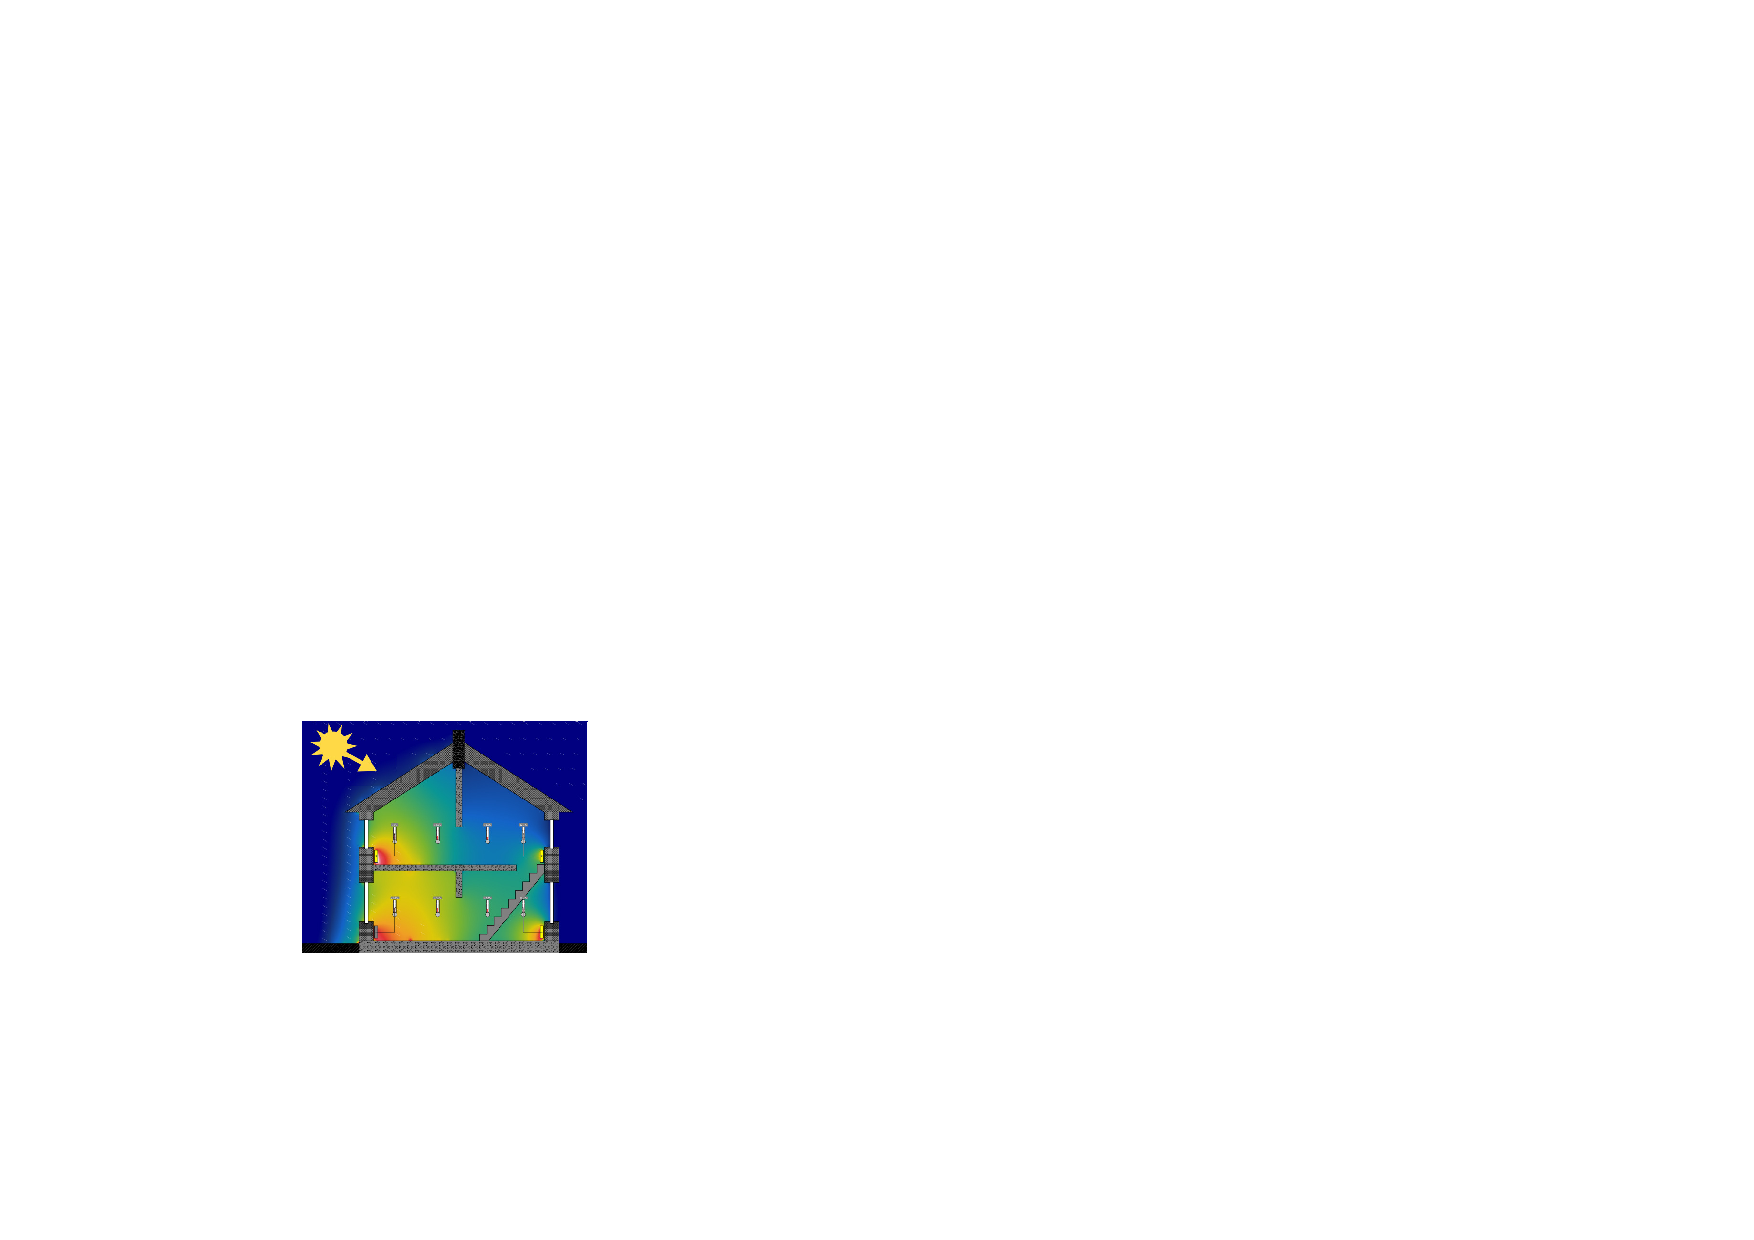
\includegraphics[width=\textwidth]{house-heating/even_powers.pdf}
		\caption{Radiator powers set evenly}
	\end{subfigure}
	~~~~ %\hspace{40pt}
		\begin{subfigure}[t]{0.47\textwidth}
			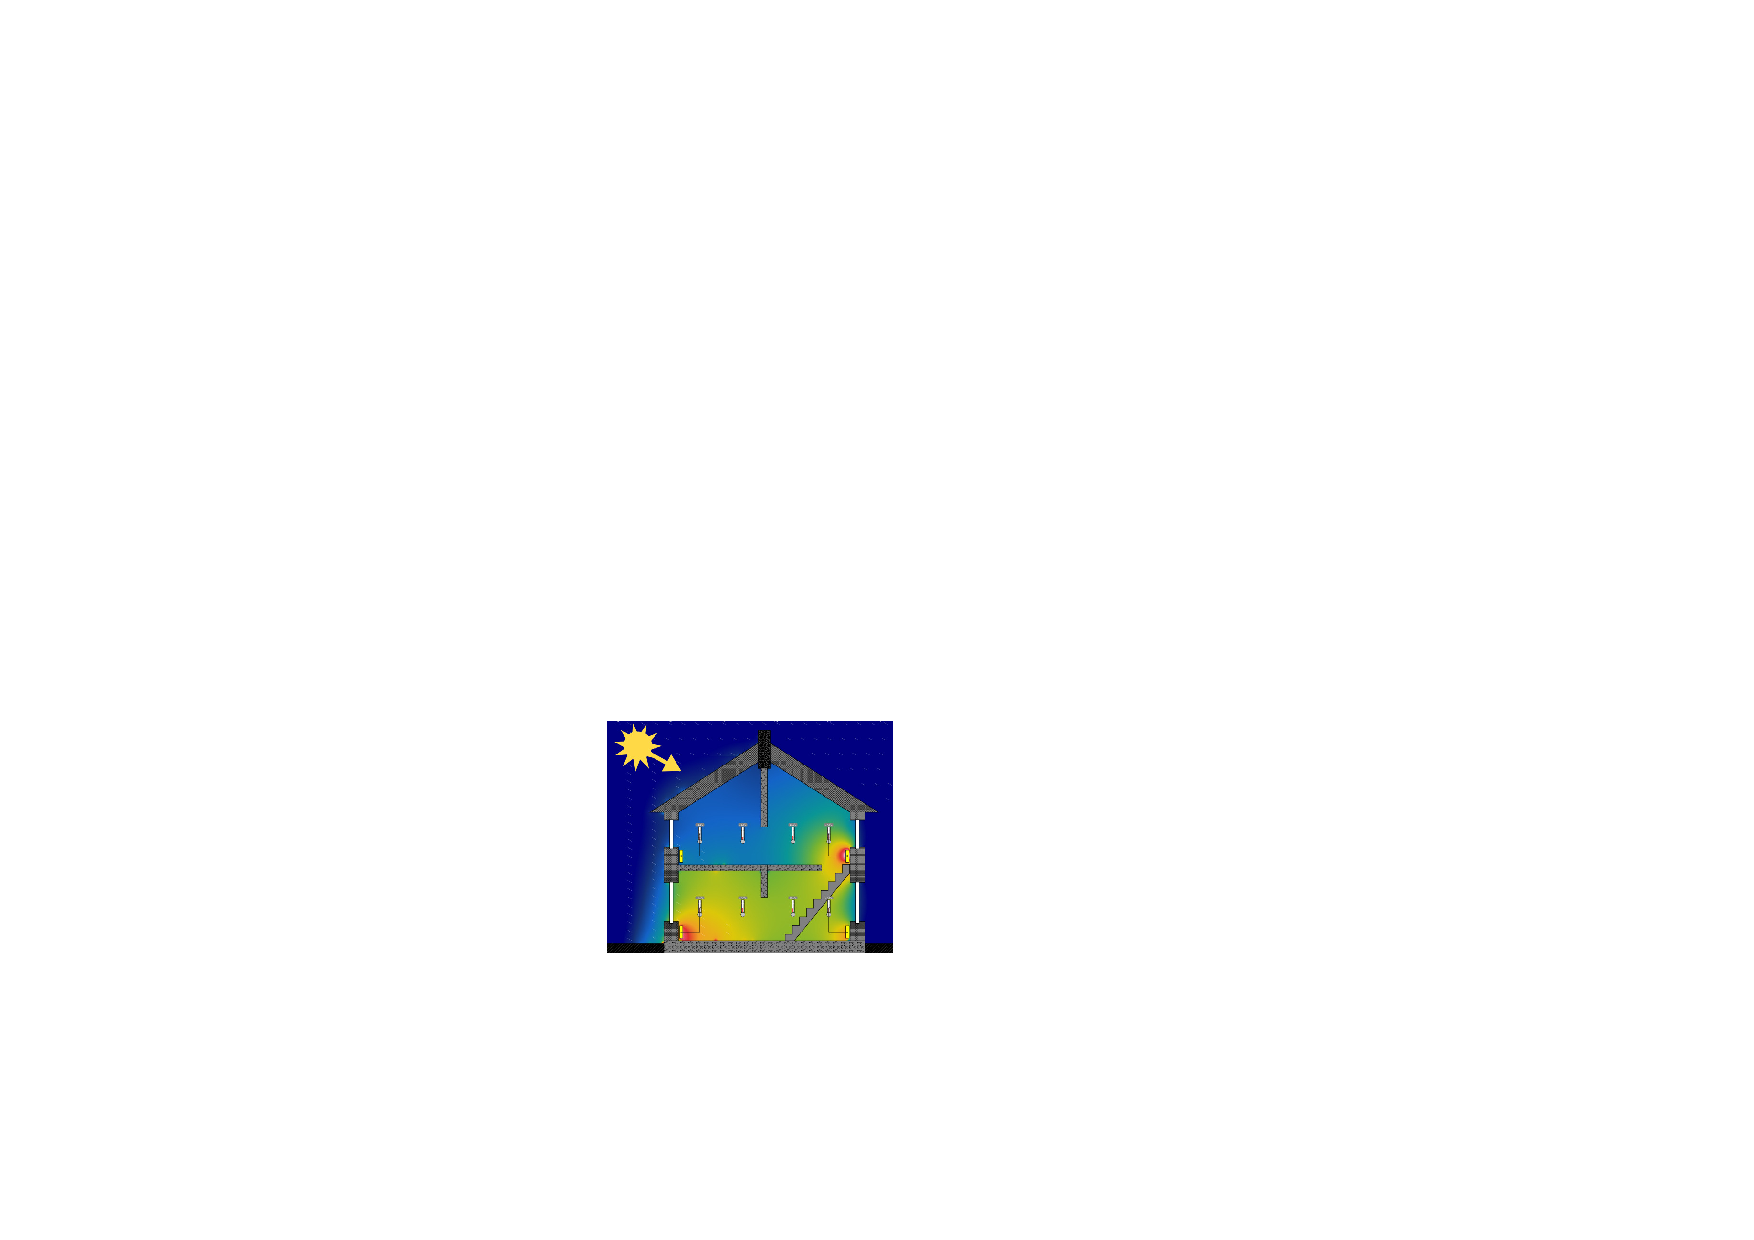
\includegraphics[width=\textwidth]{house-heating/first_iter.pdf}
			\caption{Best setup from BOPP initialization}
		\end{subfigure} \\
		\vspace{10pt}
			\begin{subfigure}[t]{0.47\textwidth}
				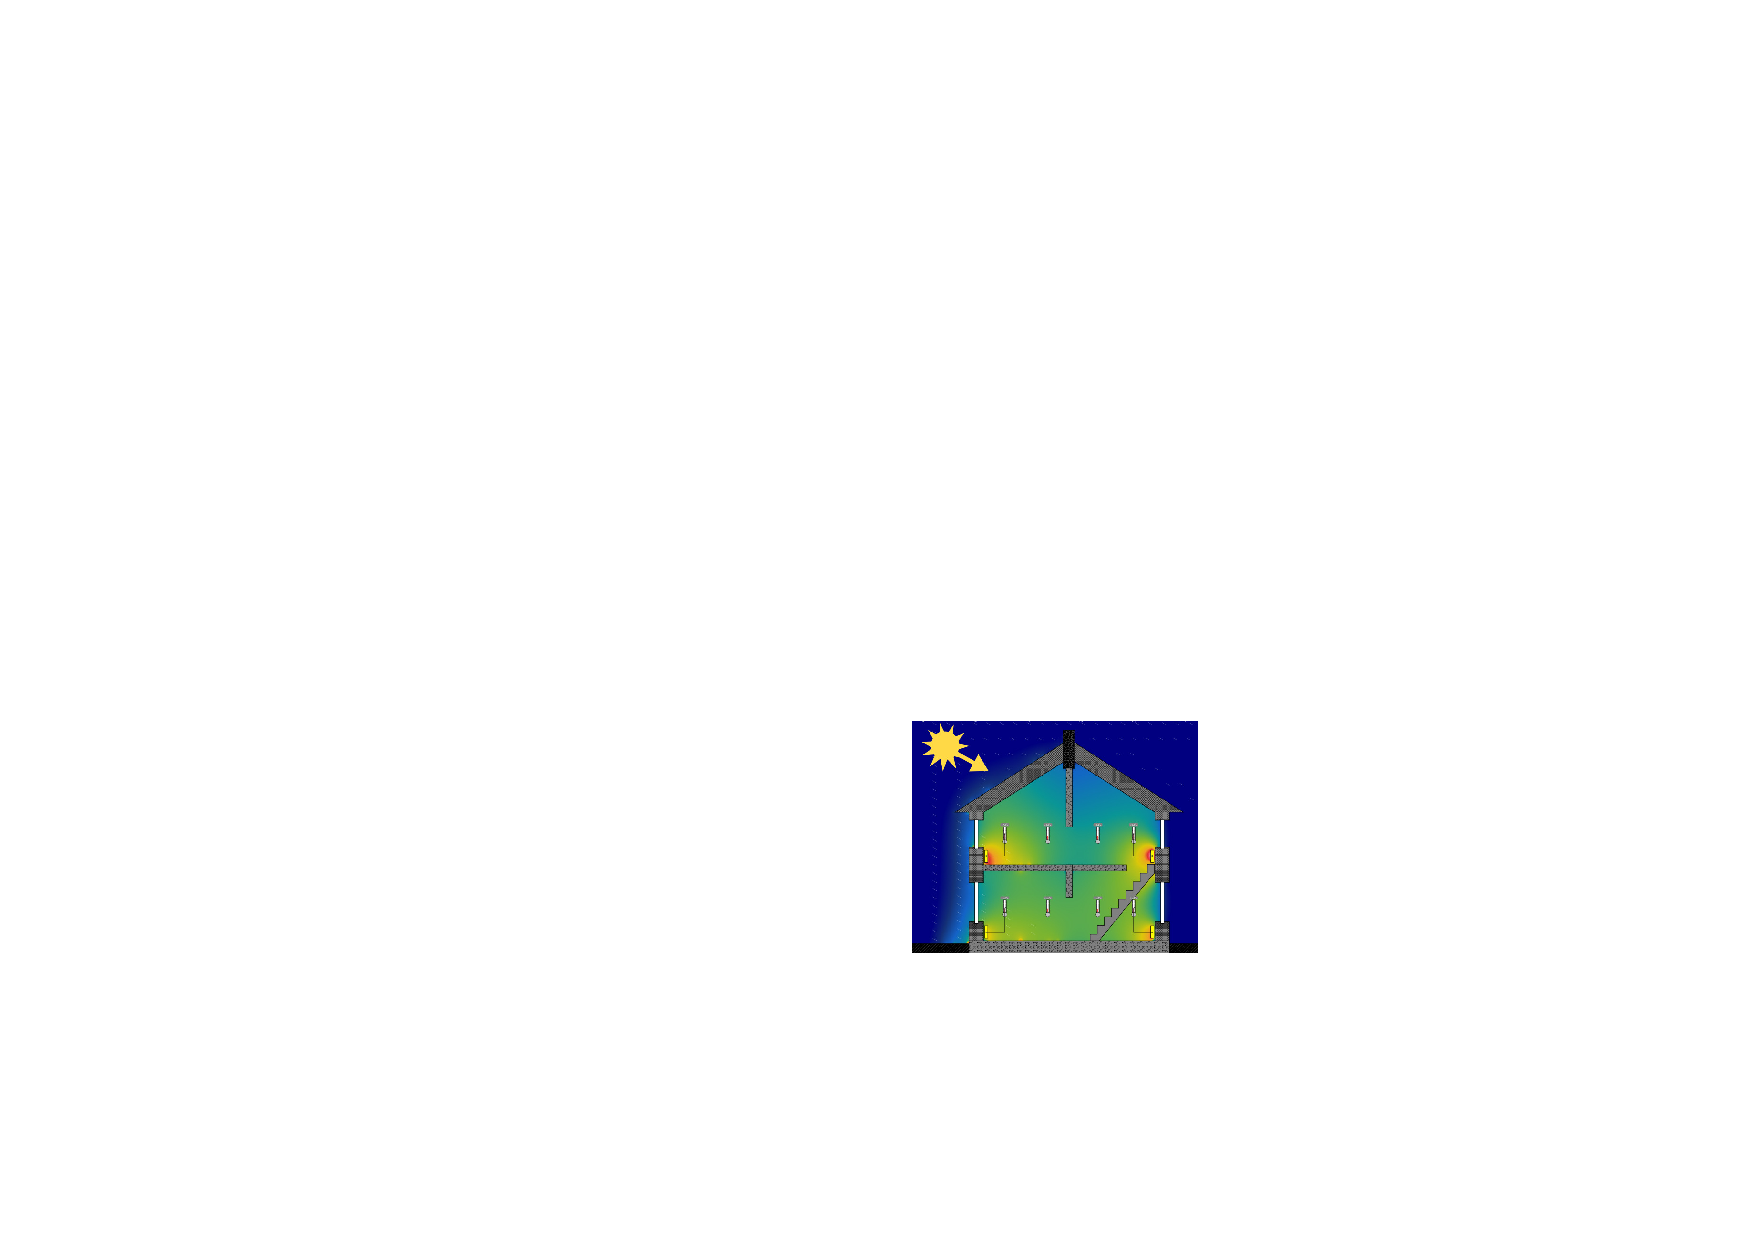
\includegraphics[width=\textwidth]{house-heating/100_iters.pdf}
				\caption{Best setup after 100 iterations of BOPP}
			\end{subfigure}
		~~~~ %	\hspace{40pt}
			\begin{subfigure}[t]{0.47\textwidth}
				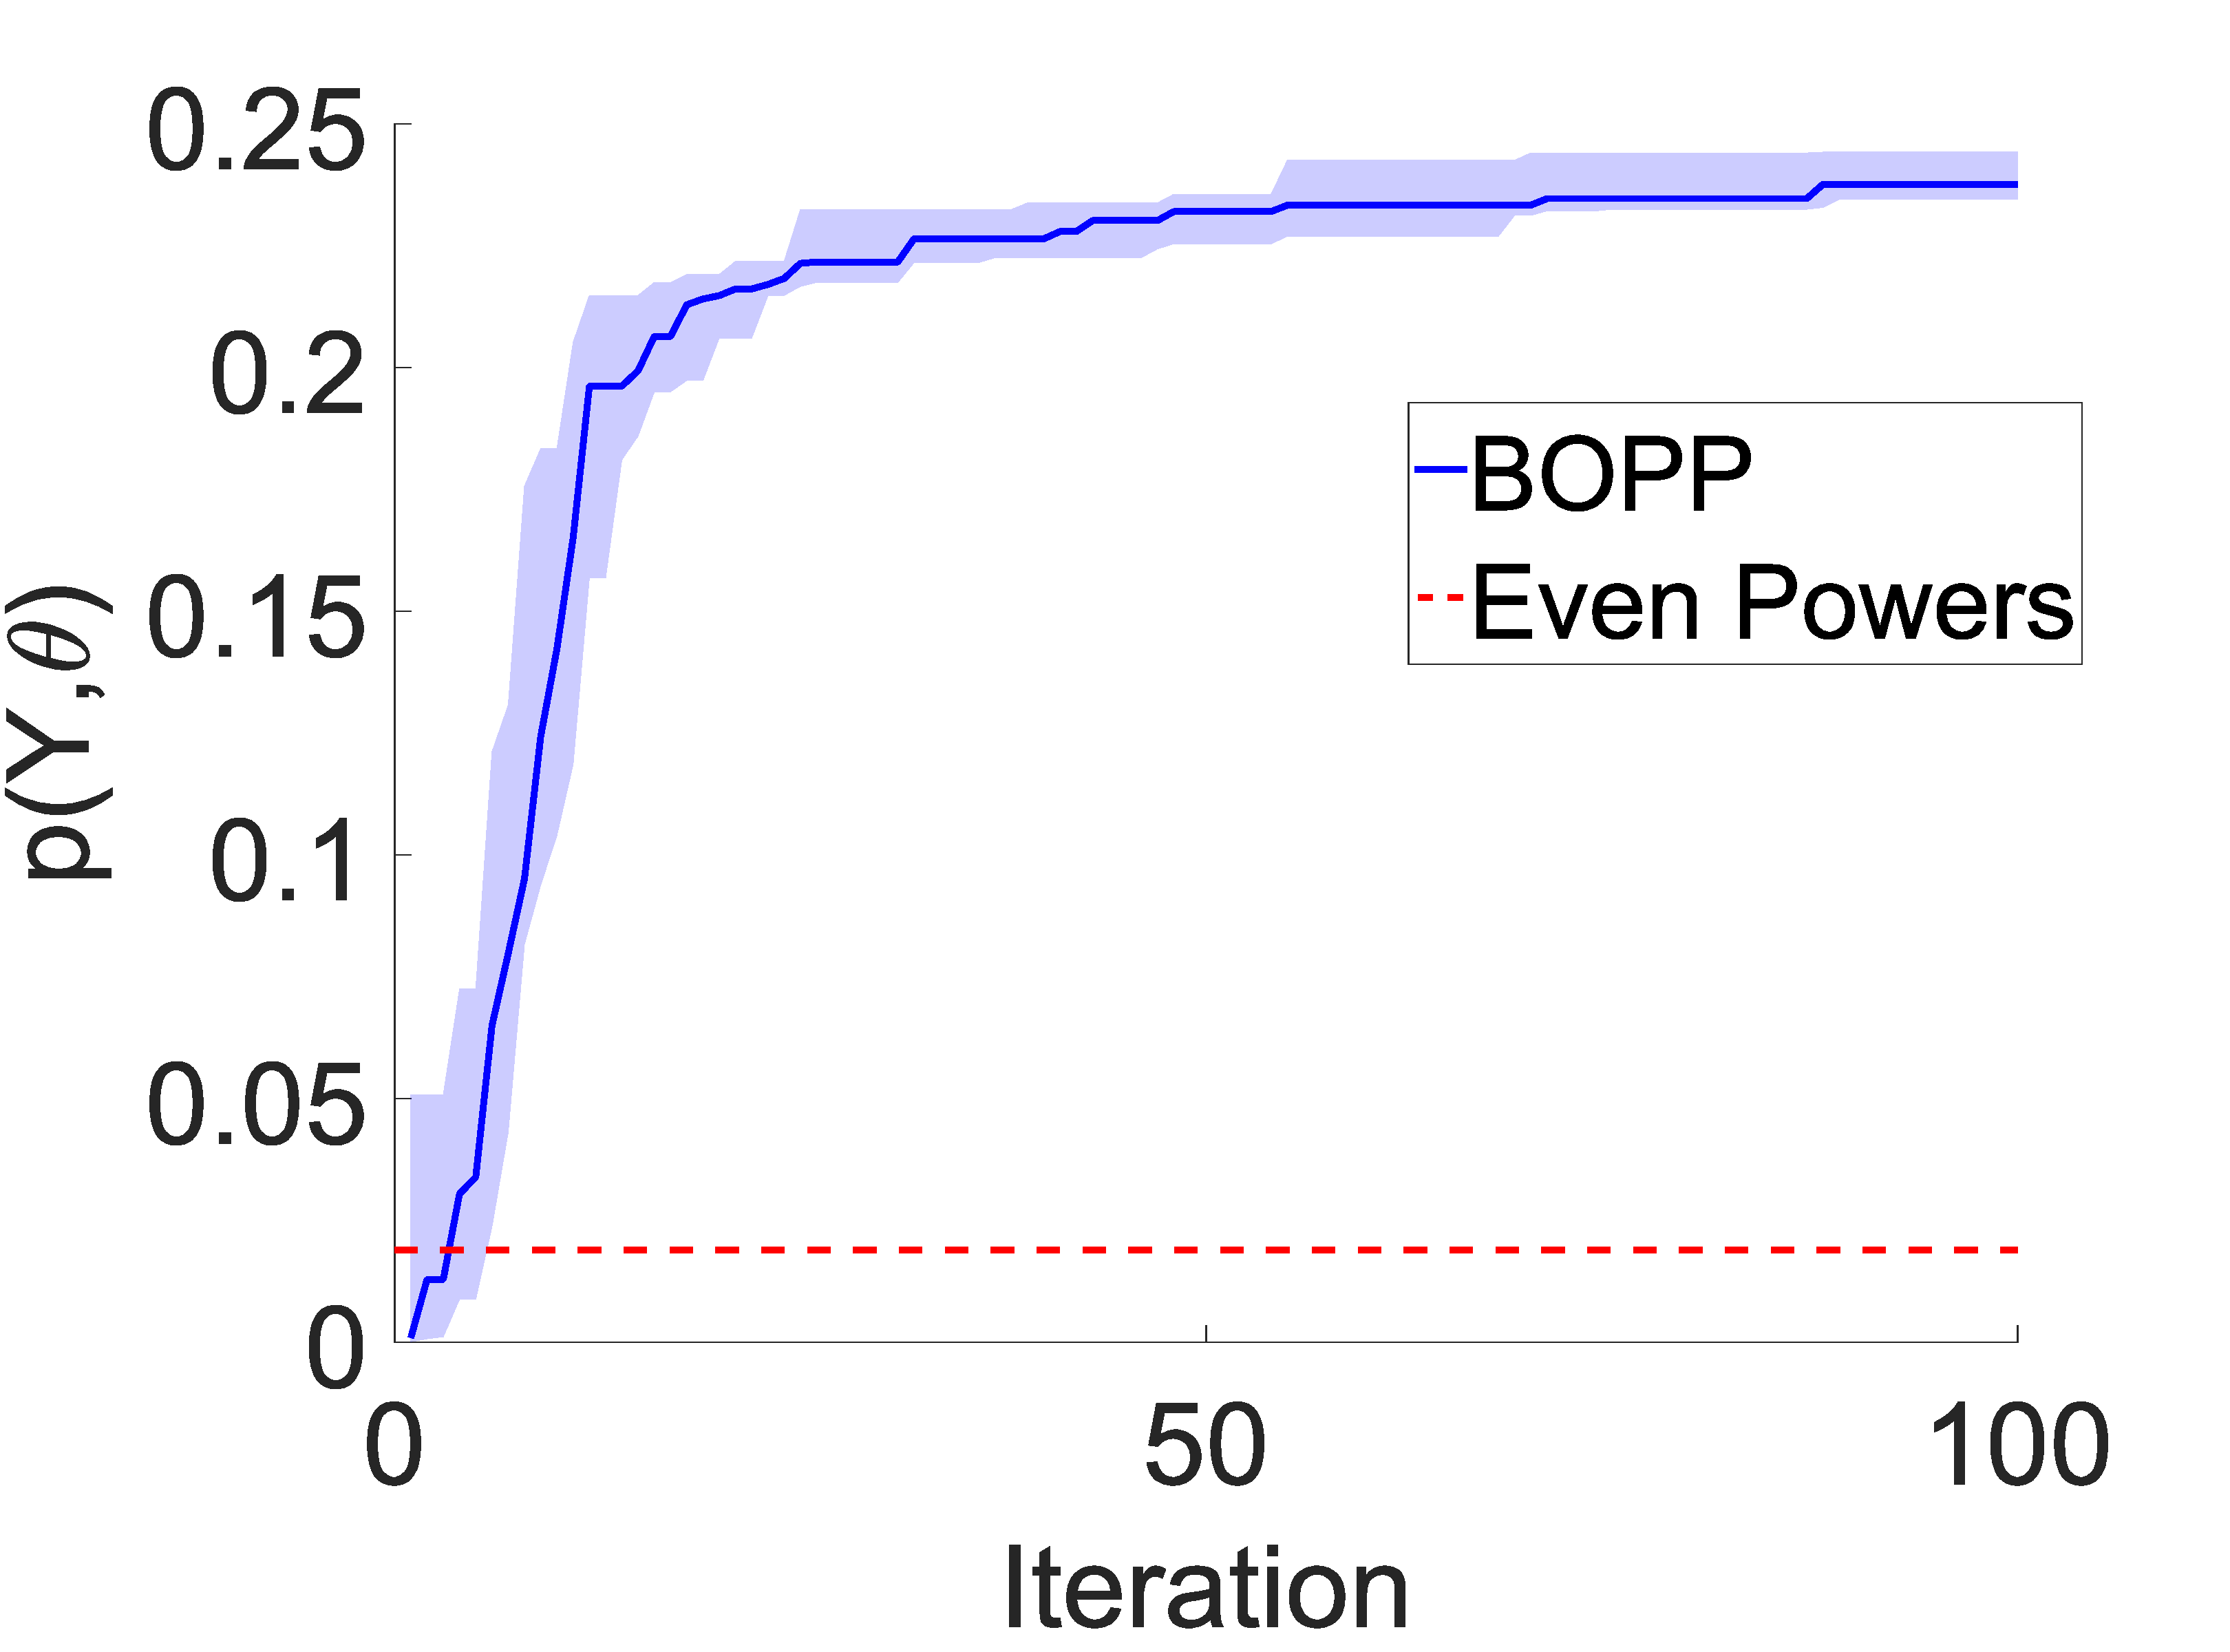
\includegraphics[width=\textwidth]{house-heating/heating_rerun.pdf}
				\caption{Convergence of evidence}
			\end{subfigure}
	% \centering ~~~
	% \includegraphics[width=0.24\textwidth]{"figures/house-heating/probabilistic/logZ-with-even-redblue-wide"}
	%			\caption{
	%				\label{fig:houses-convergence}
	%				Log marginal likelihood $\log Z$ for the \lsi{house-heating} query in Figure~\ref{fig:house-heating-code}. 
	%			}
	%	
	\caption{
		\label{fig:houses}
		Simulation-based optimization of radiator powers subject to varying solar intensity. Shown are output heat maps from Energy2D \citep{xie2012energy2d} simulations at one intensity, corresponding to setting all the radiators to the same power (\emph{top left}), the best result from a set of 5 randomly chosen powers used for initializing BOPP (\emph{top right}), and the best setup found after 100 iterations of BOPP (\emph{bottom left}). The bottom right plot shows convergence of the evidence of the respective model, giving the median and 25/75\% quartiles.
		%Simulation-based optimization of the radiator power subject to varying solar intensity. Here (a-c) show output heat maps from Energy2D \citep{xie2012energy2d} simulations, corresponding respectively to setting all the radiators to the same power, the best result from a set of randomly chosen initializations and the best setup found after 100 iterations of BOPP. (d) shows convergence of the evidence of the respective model as a function of simulation evaluations for independent restarts.
		%Homogenizing the temperature of a 2D model of a house using BOPP. The house has four adaptively controlled radiators, with additional uneven eating is provided by the sun, which will vary both temporally and probabilistically.  Our aim is to select the base power for each of the radiators, subject to some total energy budget, whilst marginalizing out the different anticipated weather conditions.  To do this, the BOPP query given in Figure \ref{fig:house-heating-code} wraps around the finite element heat transfer simulation engine Energy2D \citep{xie2012energy2d} and performs the required MMAP estimation. The na\"ive strategy of setting the power densities of the radiators uniformly (\emph{far left}) leads to an uneven heating\protect\footnotemark, noting that the colormap on the top indicates temperature of air from $5^{\circ}\mathrm C$ to $35^{\circ}\mathrm C$.  
		%After a single iteration of BOPP (\emph{middle left}), the found solution is also poor, but after 100 iterations (\emph{middle right}), a significantly improved solution has been achieved.  The log marginal likelihood in terms of iterations of number of heating setups tested is shown (\emph{far right}) for five separate BOPP runs, along with the resulting marginal likelihood from na\"ively setting the radiators to the same power.
		%Imagine that we have a number of rooms each containing a heating element and we wish to optimize the relative powers of the heaters to deliver the most uniform heating of the house over its lifetime given some total energy budget.  
		% For example, the sun will apply uneven heating to house in a manner which various over time, e.g. due to weather changes and variations in the arc of the sun through the year.  BOPP provides a basis to naturally incorporate these uncertainties into the model, whilst still exploiting the original finite element simulation and returning a single solution the engineer can the go implement.  We therefore believe that in the long term, PPS supporting MMAP have the potential to revolutionise the manner in which engineering simulation is approached by incorporating uncertainty from all stages of the process into a single unified framework, reducing the reliance on fudge-factors and educated guesswork.
	}
\end{figure*}

\begin{figure}[tb]
	\begin{lstlisting}[basicstyle=\ttfamily\small]
(defopt house-heating [alphas target-temperatures] [powers]
 (let [solar-intensity (sample weather-prior)
       powers (sample (dirichlet alphas))
       temperatures (simulate solar-intensity powers)]
  (observe (abc-likelihood temperatures) target-temperatures)))
	\end{lstlisting}	
	\vspace{-6pt}
	\caption{BOPP query for optimizing the power allocation to radiators in a house.  Here \lstinline{weather-prior} is a distribution over the solar intensity and a uniform Dirichlet prior with concentration \lsi{alpha} is placed over the powers. Calling \simulatec performs an Energy2D simulation of house temperatures. The utility of the resulting output is incorporated using \abcl, which measures a discrepency from the \texttt{target-temperatures}. Calling \doopt on this query invokes the BOPP algorithm to perform MMAP estimation, where the second input \lstinline{powers} indicates the variable to be optimized. \label{fig:house-heating-code}}
\end{figure}

Figure~\ref{fig:houses} illustrates how BOPP can be applied to engineering design, taking the example of optimizing the distribution of power between radiators in a house so as to homogenize the temperature, while marginalizing out possible weather conditions and subject to a total energy budget. The probabilistic program shown in Figure~\ref{fig:house-heating-code} allows us to define a prior over the uncertain weather, while conditioning on the output of a deterministic simulator (here Energy2D \citep{xie2012energy2d}-a finite element package for heat transfer) using an ABC likelihood.  BOPP now allows the required coincident inference and optimization to be carried out automatically, directly returning increasingly optimal configurations. 

BO is an attractive choice for the required optimization in MMAP as it is typically efficient in the number of target evaluations, operates on non-differentiable targets, and incorporates noise in the target function evaluations.  However, applying BO to probabilistic programs presents challenges, such as the need to give robust performance on a wide range of problems with varying scaling and potentially unbounded support.  Furthermore, the target program may contain unknown constraints, implicitly defined by the generative model, and variables whose type is unknown (i.e. they may be continuous or discrete).

On the other hand, the availability of the target source code in a PPS presents opportunities to overcome these issues and go beyond what can be done with existing BO packages.  BOPP exploits the source code in a number of ways, such as optimizing the acquisition function using the original generative model to ensure the solution satisfies the implicit constaints, performing adaptive domain scaling to ensure that GP kernel hyperparameters can be set according to problem-independent hyperpriors, and defining an adaptive non-stationary mean function to support unbounded BO. 

Together, these innovations mean that BOPP can be run in a manner that is fully black-box from the user's perspective, requiring only the identification of the target variables relative to current syntax for operating on arbitrary programs. We further show that BOPP is competitive with existing BO engines for direct optimization on common benchmarks problems that do not require marginalization.

%that can be implemented in any PPS where inference methods return marginal likelihood estimates. 



%MMAP estimation is generally difficult as it corresponds to the optimization of an intractable integral, such that function evaluations are expensive and give noisy results.  Current PPS inference engines are typically unsuited to such optimization.  We therefore introduce BOPP (Bayesian optimization for probabilistic programs) which couples existing inference algorithms with a new Gaussian process (GP) \citep{rasmussen2006gaussian} based Bayesian optimization (BO) \citep{osborne2009gaussian, jones1998efficient} package integrated into the PPS Anglican \citep{wood2014new}.  



%MMAP estimation for PPS presents further issues such as the need to be general purpose and robust, whilst dealing with potentially unknown constraints defined implicitly within the generative model.  


%On the other hand, the availability of the target source code in PPS presents opportunities to overcome these issues and go beyond what can be done with existing BO packages.  For example, it allows operation under unknown \emph{equality} constraints and applies automatic domain scaling for problem-independent GP hyperpriors.  In addition to delivering improved performance over prominent BO packages when used simply as an optimizer, these innovations mean that BOPP can be run in a manner that is fully black-box from the user's perspective, requiring only the identification of the target variables relative to current syntax for operating on arbitrary programs.

%\footnotetext{Though results are from the full BOPP implementation with sun heating marginalized out, the simulation plots correspond to a single common condition for the sun for visualization purposes.}

%\section{Motivating Example}
%\label{sec:motivation}


%The rest of this paper is outlined as follows: we first provide background on PPS, BO and GPs.  We define a framework for an optimization query and introduce our core code transformation to allow an arbitrary program to be optimized with respect to parameters defined within the program.  Our algorithm for optimizing the evidence of this program using BO and additional code transformations is outlined, we present experiments demonstrating the applicability of our method and we finish with concluding discussions and suggestions for future work.


\section{Related Work} 
\label{sec:bopp:related}

Reasonable consideration has been given before to solving maximum likelihood and marginal 
a posteriori (MAP) problems with PPSs and many systems provide some form of appropriate
estimation scheme (see e.g.~\citep{goodman_book_2014,carpenter2015stan,salvatier2016probabilistic}).  One simple
approach is to apply an annealing to the \observe densities (for maximum likelihood estimation)
or both the \sample and \observe densities (for MAP estimation) in
a conventional MCMC sampler such as LMH (see Section~\ref{sec:proginf:str:lmh}).
This results in a simulated annealing algorithm~\citep{aarts1988simulated} for general purpose programs.
An alternative approach, introduced by~\cite{tolpin-socs-2015}
instead uses ideas from Monte Carlo tree search to construct a general purpose MAP estimator.
However, all of these approaches do not permit the more challenging scenario
where the target is to optimize a marginal distribution.  They are, therefore, not suitable for combined
inference and optimization problems.

One approach that does consider optimization of marginal probabilities of probabilistic
programs is given by~\cite{vandemeent2016black}, which thus perhaps presents the closest
approach to our own work.  The aim of~\cite{vandemeent2016black} is, on the surface, somewhat
different to our own as they look to automate policy search problems~\citep{deisenroth2013survey}
using probabilistic programs.  However, policy search is a particular instance of MML estimation
and so falls within our general problem class.  Moreover, their approach of maximizing an evidence lower bound~\citep{blei2016variational}
using stochastic gradient ascent~\citep{robbins1951stochastic} is, in principle, substantially
more general than policy search problems and constitutes a general MML estimation scheme in its own right.
However, the approach has a number of restrictions and assumptions.  
Perhaps the most critical for our purposes is that gradients are estimated using
importance sampling and thus will generally become increasingly noisy as the dimensionality of the nuisance variables (i.e. those we wish to marginalize over) increases.
The approach also requires mean field approximations
to be made, the appropriateness of which will vary from problem to problem, while, as with other
stochastic gradient ascent approaches, a large number of optimization iterations is typically required
to reach convergence, which can be prohibitive for some problems.  BOPP, on the other hand, requires
very few assumptions to be made and is free to use more advanced inference approaches, for example
SMC, for estimating the marginal likelihood.  One consequence of this is that it can scale to far
higher dimensions in the nuisance variables.  For example, our HMM model in Section~\ref{sec:bopp:exp}
marginalizes over a roughly $5000$ dimensional space.

Another interesting alternative approach,
developed since publication of BOPP, involves taking derivatives \emph{through} an SMC
sweep~\citep{le2017auto,naesseth2017variational,maddison2017filtering}. 
More precisely, these methods allow the derivative of the marginal likelihood estimate (or more typically
its logarithm) to be calculated during an SMC sweep, for example by using automatic differentiation
on the calculation of the original estimate~\citep{le2017auto}.  This can be used for MML or MMAP estimation
of global parameters by using these gradients as input to a stochastic gradient ascent scheme.
A key difference of this approach, to say~\cite{vandemeent2016black}, is that using SMC instead of importance
sampling means that substantially lower variance gradient estimates can be achieved.
Though, to the best of our knowledge, no such approach is currently implemented in a PPS, doing so is 
in theory perfectly possible given a system supporting automatic differentiation.  
In~\cite{le2017auto}, we also show how this approach can be extended to perform simultaneous model
learning and proposal adaptation and further to an amortized inference setting, whereby we learn an inference
artifact that returns a proposal at run time.  This means that, when the model of interest comprises of
a deep neural network, then the method can be viewed as extending so-called auto-encoding methods~\citep{kingma2014auto,burda2015importance}
from their limited importance sampling setting, to a more powerful SMC framework.

\section{Problem Formulation}
\label{sec:problem}

% !TEX root =  ../main.tex

As we explained in Section~\ref{sec:probprog:models:general}, probabilistic program queries
define unnormalized distributions $\gamma(x_{1:n_x},\lambda)$ on program traces
 as defined in~\eqref{eq:probprog:universal-cond}.
At a high level, our aim is to optimize with respect to some of the $x_{1:n_x}$ variables while marginalizing out
the rest, as per MMAP estimation, MML estimation, and risk minimization introduced in
Section~\ref{sec:opt:intro}.
However, formalizing what we mean by ``some variables'' is less trivial than it would
first appear and will require specialist syntax for specifying models.  To this end,
we introduce a new query macro \defopt.  The syntax of \defopt is identical to \defquery except 
that it has an additional input identifying the variables to be optimized.  As we will
explain later, \defopt invokes a series of code transformations to produce a number
of different Anglican queries used by BOPP.  Each of these are compiled using \query
and returned as a hash map of CPS Clojure functions that can then
be used by the BOPP back end.

A possible na\"{i}ve strategy for identifying the target variables
would be to simply predefine some subset of the \sample indices
$c \subset \mathbb{N}^+$ and optimize for $\{x_j \}_{j\in c}$.  However, this is clearly not satisfactory
because it is generally an awkward method of identifying the target variables and the variables we wish
to optimize may not always be sampled at the same position in our trace (i.e. we do not want superfluous
\sample statements to effect which variables constitute our target variables).
Unfortunately though, the more natural choice of specifying any variable in the program, including those
which are deterministic functions of other variables, is not possible in general, because of complications
originating from changes of variables, namely that nonlinear deterministic mappings change the density
function in ways that it might not be possible to track.  Instead, we will still specify our target variables
$\theta = \phi_{1:L}$ by name (i.e. using the lexical name of the variable as bound by a \clj{let} block in
the raw program code), but we will place some restrictions, enforced at run time (see~\cite{rainforth2016nips}), 
to ensure validity of the model.  First, each optimization variable $\phi_{\ell}$ must be bound to a value directly 
by a \sample statement to avoid change of variable complications.
%Specifically if $\psi = g(\theta)$ then $p(Y,\theta) = \text{\bf D}_g(\psi) p(Y,\psi)$ where $\text{\bf D}_g$ represents the Jacobian associated with $g$, giving different maxima for $\theta$ and $\psi$ \cite{murphy2012machine}.
Second, in order for the optimization to be well defined, the program must be written such that any 
possible execution trace binds each optimization variable $\phi_{\ell}$ exactly once.  By proxy, this also
ensures that the number of variables to be optimized, $L$, remains fixed.
% HOW DO WE ENFORCE THIS? 
Finally, although any $\phi_{\ell}$ may be lexically multiply bound, it must have the same reference 
measure in all possible execution traces, because, for instance, if the reference measure of 
a $\phi_{\ell}$ were to change between Lebesgue to counting, the notion of optimality would 
no longer admit a conventional interpretation.  Note that we impose no restrictions on the latent
variables which will be marginalized over.

From a developer's perspective, these minor restrictions mean that all \sample statements are
either associated with a particular target variable $\phi_{\ell}$ or never associated with any target 
variable. Further, \sample
statements associated with the target variables will never be evaluated more than once (but might never
be evaluated if there are multiple possible \sample statements associated with a particular $\phi_{\ell}$) and
the total number of \sample statements associated with the target variables is always $L$.
Therefore building on the notation from Section~\ref{sec:probprog:models:general}, we will redefine $x_{1:n_x}$
as the variables that are to be marginalized over, with all associated terms similarly redefined (except $\gamma$).
We next denote the $m_{\ell}$ lexical \sample statements associated with $\phi_{\ell}$ as 
$h_{\ell,1},\dots,h_{\ell,m_{\ell}}$ with associated density functions $h_{\ell,i}(\phi_{\ell} | \xi_{\ell})$ where
$\xi_{\ell}$ is the provided distribution object (which can be a random variable but its reference measure
must be deterministic).  We further denote $c_{\ell} \in \{1,\dots,m_{\ell}\}, \; 
\forall \ell \in \{1,\dots,L\}$ as the (potentially random) variable used to index which lexical \sample statement
$\phi_{\ell}$ is drawn from in a particular execution.  We now have that the conditional distribution on the trace $\mT$ implied
by the query is $p(\mT = \{\phi_{1:L},x_{1:n_x}\} | \lambda) \propto \gamma(\theta,x_{1:n_x}, \lambda)$
where
\begin{align}
\label{eq:bopp:joint}
\gamma(\theta,x_{1:n_x}, \lambda) = \begin{cases}
\prod_{\ell=1}^{L}
h_{\ell,c_{\ell}} (\phi_{\ell} | \xi_{\ell})
\prod_{j=1}^{n_x} 
f_{a_j}(x_j | \eta_j)
\prod_{k=1}^{n_y}
g_{b_k}(y_k | \psi_k) \;\;\; \text{if} \;\;\; \mathcal{B}(\theta,x_{1:n_x},\lambda)=1 \\
0 \quad \text{otherwise}
\end{cases}
\end{align}
and we have redefined the trace validity function $\mathcal{B}(\phi_{1:L},x_{1:n_x},\lambda)$ appropriately.
As before, although many of the terms in our trace probability are random variables, all are deterministic
functions of $\{\phi_{1:L},x_{1:n_x}\}$.  Note that the relative ordering of the $\phi_{1:L}$ to the $x_{1:n_x}$
does not affect the validity of the trace or the probability, as the \sample statements associated with
each are mutually exclusive.

We can now use~\eqref{eq:bopp:joint} to define the MMAP estimate targeted by a \defopt query as
\begin{align}
\label{eq:bopp:mmap}
\begin{split}
\theta^*& (\lambda) = \argmax_{\theta \in \vartheta (\lambda)} 
\E \left[p(\mT = \{\phi_{1:L},x_{1:n_x}\} | \lambda) \middle| \theta \right]
= \argmax_{\theta \in \vartheta (\lambda)} 
\E \left[\gamma(\theta,x_{1:n_x}, \lambda) \middle| \theta \right] \\
& = \argmax_{\theta \in \vartheta (\lambda)} 
\int_{x_{1:n_x} \in \{X : \mathcal{B}(\theta,X,\lambda)=1\}} 
\prod_{\ell=1}^{L} h_{\ell,c_{\ell}} (\phi_{\ell} | \xi_{\ell})
\prod_{j=1}^{n_x} f_{a_j}(x_j | \eta_j) \prod_{k=1}^{n_y} g_{b_k}(y_k | \psi_k) dx_{1:n_x}
\end{split}
\end{align}
where $\vartheta (\lambda) := \{\theta : \exists x_{1:n_x} : \gamma(\theta,x_{1:n_x},\lambda)>0\}$
is the support of $\theta$ given $\lambda$.  
For simplicity and notational consistency with our original paper~\citep{rainforth2016nips}, 
we will now drop the dependency on $\lambda$ in the rest of the paper and instead
use the notation for MMAP estimation of a graphical model given in~\eqref{eq:opt:MMAP}
(such that we express the MMAP problem as $\theta^* = \argmax_{\theta \in \vartheta}
p(Y,\theta)$),
where $Y$ represents data and $X$ are variables marginalized over, noting that this
is not always completely accurate as per Section~\ref{sec:probprog:models:general} and 
\eqref{eq:bopp:mmap}.

To carry out the interleaving of inference and optimization required in MMAP estimation, we
introduce \doopt, which, analogous to \doquery, takes a compiled output from \defopt and
returns a lazy sequence $\{\hat{\theta}^*_m,\hat{\Omega}^*_m,\hat{u}^*_m\}_{m=1,\dots}$
where $\hat{\Omega}^*_m \subseteq X$ are the program outputs associated with
$\theta=\hth^*_m$ and each $\hat{u}^*_m \in \real^+$ is an estimate of the corresponding
log partition function $\log p(Y, \hth_m^*)$ (see Section \ref{sec:bopp-for-ml}).  The
sequence is
defined such that, at any time, $\hat{\theta}^*_m$ corresponds to the point expected to be
most optimal of those evaluated so far and allows both inference and optimization to be
carried out online.


\section{Bayesian Program Optimization}
\label{sec:bopp}

% !TEX root =  ../main.tex

On top of the syntax introduced in the previous section, there are five main components to BOPP:
\vspace{-5pt}
\begin{itemize}
	\setlength\itemsep{-0.2em}
	\item[-] A program transformation, \clj{q}$\rightarrow$\qmarg, allowing estimation of the partition function $p(Y,\theta)$ at a fixed $\theta$.
	\item[-] A bespoke, GP based, BO implementation for actively sampling $\theta$.
	\item[-] A program transformation, \clj{q}$\rightarrow$\qprior,  used for automatic and adaptive domain scaling, such that a problem-independent hyperprior can be placed over the GP hyperparameters.
	\item[-] An adaptive non-stationary mean function to support unbounded optimization.
	\item[-] A program transformation, \clj{q}$\rightarrow$\qacq, and maximum likelihood estimation method to optimize the acquisition function subject the implicit constraints imposed by query.
\end{itemize}
\vspace{-5pt}
Together these allow BOPP to perform online MMAP estimation for arbitrary programs in a manner that is black-box from the user's perspective -- requiring only the definition of the target program in the same way as existing PPS and identifying which variables to optimize.  The BO component of BOPP is both probabilistic programming and language independent, and is provided as a stand-alone package.  It requires as input only a target function, a sampler to establish rough input scaling, and a problem specific optimizer for the acquisition function that imposes the problem constraints.  %We first provide a high-level overview of the algorithm before separately explaining these components.

%BOPP provides online MMAP estimation for arbitrary programs in a manner that is black-box from the user's perspective - requiring only the definition of the target program in the same way as existing PPS and identifying which variables to optimize. It has three main components: a series of program transformations, inference schemes for evaluating these transformed programs, and a BO scheme that uses them to provide the required MMAP estimation.  Implementation of the transformations is naturally language specific, but the required techniques can be applied to any system with general-purpose languages for model specification and which provides the required inference schemes.  Given functions for evaluating these transformed programs, the BO scheme for MMAP estimation can be abstracted from probabilistic programming and is provided as its own separate package\footnote{\url{http:\\www.bitbucket.org\twgr\bo-mapp}}.  This package requires three things: a target function which provides estimates of the marginal $p(Y,\theta)$, a sampler for cheaply generating a rough representation of the input scaling, and an optimizer for the acquisition function that imposes the constraints of the problem.

\begin{figure}[t]
	\centering
	\includegraphics[width=\textwidth]{"bopp_overview_figure"}
	%\vspace{20pt}
	\caption{
		\label{fig:bopp_overview}
		Overview of the BOPP algorithm, description given in main text. \clj{p-a}, \lsi{p-}$\theta$, \lsi{p-b} and \lsi{lik} all represent distribution object constructors.
		\lsi{observe<-} is identical to \lsi{observe} except it returns the observation. \lsi{factor} is a special distribution constructor that here factors the trace probability by $\zeta(\theta)$. }
\end{figure}

Figure \ref{fig:bopp_overview} provides a high level overview of the algorithm invoked when \doopt is called on a query \clj{q} that defines a distribution $p\left(Y, a, \theta , b\right)$.  We wish to optimize $\theta$ whilst marginalizing out $a$ and $b$, as indicated by the the second input to \clj{q}. In summary, BOPP performs iterative optimization in 5 steps
\begin{description}[align=left]
	\setlength\itemsep{-0.1em}
	\item[Step 1] (\emph{blue arrows}) generates exact samples from the prior program \clj{q-prior} (\emph{top center}), constructed by removing all conditioning. This initializes the domain scaling for $\theta$.
	\item[Step 2] (\emph{red arrows}) evaluates the marginal $p(Y,\theta)$ at a small number of the generated $\hth$ by performing inference on the marginal program \qmarg~ (\emph{middle center}), which returns samples from the distribution $p\left(a,b | Y, \theta\right)$ along with an estimate of $\log p(Y, \theta)$.  The evaluated points (\emph{middle right}) provide an initial domain scaling of the outputs and starting points for the BO surrogate.
	\item[Step 3] (\emph{black arrow}) fits a mixture of GPs posterior
	to the scaled data (\emph{bottom centre}) using a problem independent hyperprior. The solid blue line and shaded area show the posterior mean and $\pm2$ standard deviations respectively. The new estimate of the optimum $\hth^*$ is the value for which the mean estimate is largest, with $\hat{u}^*$ equal to the corresponding mean.    
	\item[Step 4] (\emph{purple arrows}) constructs an acquisition function $\zeta \colon \vartheta \rightarrow \real^+$ (\emph{bottom left}) using the GPs.  This is optimized, giving the next point to evaluate $\hth_{\mathrm{next}}$, using simulated annealing on a transformed program \clj{q-acq} (\emph{middle left}) in which all \observe statements are removed and replaced with a single \observe adding a $\zeta(\theta)$ factor to the trace probability. % A non-stationary prior mean function for the GP, the AF is penalized away from a region of interest, allowing unbounded optimization.  
	%The AF is optimized by performing annealed importance sampling on a transformed program \clj{q-acq} (\emph{middle left}) in which all \observe statements are removed and replaced with a single \observe that assigns probability $\zeta(\theta)$ to the execution. 
	\item[Step 5] (\emph{green arrow}) evaluates $\hth_{\mathrm{next}}$ using \qmarg~and continues to step 3.
\end{description}

\subsection{Program Transformation to Generate the Target}
\label{sec:transform}
% !TEX root =  ../main.tex

Consider the \defopt query \texttt{q} in Figure \ref{fig:bopp_overview}, the body of which defines the joint distribution $p\left(Y,a,\theta,b\right)$.   Calculating~\eqref{eq:opt:MMAP} (defining $X=\left\{a,b\right\}$) using a standard optimization scheme presents two issues: $\theta$ is a random variable within the program rather than something we control and its probability distribution is only defined conditioned on $a$.

We deal with both these issues simultaneously using a program transformation similar to the disintegration transformation in Hakaru \citep{zinkov2016composing}. Our \emph{marginal} transformation can be thought of generating a new query, \qmarg~ as shown in Figure~\ref{fig:bopp_overview}, that defines the same unnormalized joint distribution on program variables and inputs (i.e. $\gamma(\theta,x_{1:n_x},\lambda)$ is unchanged), but now accepts the value for $\theta$ as an input (i.e. the $\phi_{1:L}$ become terms in $\lambda$ rather than being random variables).  As such, the partition function of the program is
now a function of $\theta$ and therefore can be optimized using an external algorithm.
The transformation itself replaces all \sample statements associated with each $\phi_{\ell}$ with an equivalent \observes statement, taking $\phi_{\ell}$ as the observed value, where \observes is identical to \observe except that it returns the observed value instead of \clj{nil}.  As both \sample and \observe operate on the same variable type -- a distribution object -- this transformation can always be made, while the identical returns of \sample and \observes trivially ensures validity of the transformed program.  The transformation used for MML and risk
minimization
is equivalent except that the \observe statements are replaced by an identity function (rather than \observes), such
that the transformation effectively removes the original \sample statements.

In truth, the transformations used by BOPP are not exactly as shown in~\ref{fig:bopp_overview}
and as described above.  This is because, although for simple programs, such as the given
example, these transformations can be easily expressed as static transformations, for more
complicated programs it would be difficult to actually implement these as purely static
generic transformations in a higher-order language.  Therefore, even though all the
transformations dynamically execute as shown at runtime, in truth, the generated source 
code for the prior and acquisition transformations varies from what is shown and has 
been presented this way in the interest of exposition.  Our true transformations exploit
the existing Anglican special forms \lsi{store} and \lsi{retrieve} and two new
special forms we introduce called \lsi{catch} and \lsi{throw}, in order to generate programs
that dynamically execute in the same way at run time as the static examples shown, but
whose actual source code varies significantly.  Full details are given in~\cite{rainforth2017boppArxiv}.

%We now build upon our optimization query to demonstrate how BOPP can optimize with respect to an arbitrary subset of variables sampled within a PP.  This is equivalent to optimizing with respect to an arbitrary subset of nodes in a graphical model, whilst marginalizing over the others, representing a new method beyond the scope of current BO algorithms.


%Consider the Anglican query \texttt{q} in figure \ref{fig:originalQuery} as a demonstrative example.  The marginal distribution defined by \texttt{q}, $p\left(Y,\theta\right) = \int_{U} \int_{V} p\left(U\right)p\left(\theta|U\right)p\left(V|\theta,U\right)p\left(Y|V,\theta,U\right)dUdV$, is the same objective function as in~\eqref{eq:hyperOpt} if we define $X= \left\{U,V\right\}$, but $\theta$ is no longer at the root of the dependency structure as it was in \eqref{eq:Joint}.  This causes two problems for optimizing with respect to $\theta$: it is sampled within the program and the corresponding probability distribution is only defined conditioned on one of the parameters we wish to marginalize over $U$.  

%We propose dealing with both these issues simultaneously using a program transformation by which we change any \sample statements for elements of $\theta$ into \observes statements, resulting in the transformed query \texttt{qT} shown in \ref{fig:transformedQuery}.  Here \observes is identical to \observe except that its return value is equal to its observation, in this case $\theta$.  The transformed query is a function of $\theta$ and can therefore be optimized.  When \doquery is called on \texttt{q} with the BOPP algorithm specified as the inference engine, it acts a macro which first makes this transformation before passing the transformed program to our BO wrapper.

%At a high level, the result of this transform is that we use use the defined probability distribution for sampling $\theta$ to condition the program to a particular value of $\theta$.  Critically, the distribution defined by the program has not changed.  This is easiest to assert by considering the program as defining a joint density on the sampled variables and the observations, and noting that whether these variables are fixed or sampled at runtime does not change the definition of this joint.  This simple but elegant solution means that we can transform any probabilistic program, and therefore any graphical model, to an optimization problem with respect to any of its sampled variables. 





%\subsection{Marginal Maximum A Posteriori Estimation}
%% !TEX root =  bopp.tex

%In this section we introduce a set of requirements for an ``optimization query", which returns an infinite lazy sequence of increasingly optimal estimates for some target variables $\theta \in \vartheta$.  For exposition purposes, we first consider the case where $\theta$ correspond to the inputs of a query $q$ and show how this can be extended to arbitrary variables within the program in section \ref{sec:transform}. We assume $q$ takes as inputs, along with $\theta$ data upon which the query is conditioned $Y$.


%As it is only possible to estimate $p(Y, \hth_m)$ such that
%\begin{align}
%\label{eq:BOPPoutput}
%E_f\left[\hat{p} \left(Y,\hth_m\right) | D_{m} \right] \ge E_f\left[\hat{p} \left(Y,\hth_j\right) | D_{m} \right] \quad \forall j=1,\dots,m-1
%\end{align}
%where $\hat{p}$ is used to indicate that the estimation of the marginal probability is itself probabilistic due to the approximation nature of inference. 

Given the above program transformation we can use a generic inference method provided by the back end to marginalize over the latent variables $X$ conditioned on $\theta$. We will here use sequential Monte Carlo for probablistic programs \citep{wood2014new} to obtain unnormalized estimates of the marginal conditional likelihood
\begin{align}
\hw \left(Y,\theta\right) \approx p\left(Y | \theta\right) =\int p\left(X,Y|\theta\right) dX.
\end{align}
Given these estimates we are now in a position to define the problem setting for MMAP estimation in probabilistic programs. Specifically we will define a macro \lsi{doopt} that accept a query defined using \lsi{defopt} and returns a lazy sequence of increasingly optimal estimates for the target variables $\theta$. We now formally define our optimization query to output an infinite lazy sequence $\{\hth_1,\hat{\Omega}_1\},\{\hth_2,\hat{\Omega}_2\},\dots$ where $\hat{\Omega}_i$ is the map of \predict values with the query when $\theta=\hth_i$ and
\begin{align}
\label{eq:BOPPoutput}
E\left[\hw \left(Y,\hth_m\right) p\left(\hth_m\right) | D_{m} \right] \ge E\left[\hw \left(Y,\hth_j\right) p\left(\hth_j\right) | D_{m} \right] \quad \forall j=1,\dots,m-1 \quad m=1,2,\dots
\end{align}
where the expectation is over the surrogate function posterior. $\hth_m$ corresponds to the point that is expected to be the most optimal of those evaluated under the posterior of our surrogate function. Since evaluations of are noisy, this need not be the $\theta$ value that produced the highest the $p(\theta)$-weighted marginal likelihood estimate. % Further as the observation of a new point affects the surrogate function posterior at all other points (as the expectation of both sides of~\eqref{eq:BOPPoutput} is conditioned on all data observed so far $D_m$), $\hth_m$ can change between different historical values when a new point is queried.


% Consider a generic query $q$.  Let the \sample statements within the $q$ define a generative distribution for a set of latent variables $X = \left\{x_{i}\right\}_{i=1,\dots,N}, \; X \in \mathcal{X}$ (note $x_i$ may have different support for different $i$) with prior $p\left(X | \theta\right) = p\left(x_1 | \theta\right) \prod_{i=2}^{N} p\left(x_i | x_1,\dots,x_{i-1},\theta\right)$, parametrized by a set of program inputs $\theta \in \vartheta$.  Let the \observe statements in the program define conditioning on observations $Y = \left\{y_i\right\}_{i=1,\dots,N}, \; Y \in \mathcal{Y}$ such that the query defines the joint factorization\footnote{Note, there is notational deficiency as in a higher-order PPS variable types, the order of the conditioning for the latent variables and even the number of latent variables can change depending on the program trace.}
% \begin{multline}
% \label{eq:Joint}
% p\left(X,Y|\theta\right) = p\left(x_1 | \theta\right) p\left(y_1 | x_1, \theta\right) \\ \prod_{i=2}^{N} p\left(y_i | x_1,\dots,x_{i},\theta\right) p\left(x_i | x_1,\dots,x_{i-1},\theta\right).
% \end{multline}
% We assume that the observations $Y$ are fixed and finite dimensional.  Our aim is to optimize the marginal likelihood of this joint scaled by a prior on $\theta$:
% \begin{align}
% \label{eq:hyperOpt}
% \theta^* = \argmax_{\theta \in \vartheta} p\left(\theta\right) \int_{X}^{} p\left(X,Y|\theta\right) dX,
% \end{align}

%Often the prior on $\theta$ will often correspond only to a set of bounds, giving a uniform distribution within the permissible input space.  If $p\left(\theta\right)$ is allowed to be potentially improper,~\eqref{eq:hyperOpt} also incorporates maximum likelihood estimation .  
%restricting the choice of inference algorithm. Anglican supports a number of suitable algorithms including importance sampling \citep{glynn1989importance}, sequential Monte Carlo (SMC) \citep{smith2013sequential,wood_aistats_2014} and the particle cascade \citep{paige2014asynchronous}.


For clarity we introduce the following notation of the rest of the paper.  We use $\theta_m$ to refer to the $\theta$ used to call the query at iteration $m$, and $\Omega_m$ and $W_m$ for the predicts and marginal likelihood estimate from this call respectively.  We define $\jsm \in \{1,\dots,m\}$ to be the index corresponding to the estimated best $\theta_m$ at iteration $m$ such that $\hth_m = \theta_{\jsm}$.  We further define $Z_m \coloneqq W (Y,\theta_j) p(\theta_j)$ and $\hz_m \coloneqq \hw (Y,\hth_j) p(\hth_j)$ as the corresponding estimates of the weighted marginal weights.

%We finally note that our optimization query includes as a special case independent calls to an inference query by setting $\ell (\cdot) = 0$ and by convention taking the most recent sample under equality of~\eqref{eq:BOPPoutput}.  Furthermore, one is free to choose the sequence of $\tilth$ in anyway desired.  For example, one may wish to explicitly control the trade off between improving our estimates for $\theta^*$, and refining the inference of the latent variables $p(z | y, \tilth_{\jsm})$ by recalling the original query with the same $\theta$.


\subsection{Bayesian Optimization of the Marginal}
\label{sec:BOPP}

% !TEX root =  ../main.tex

The target function for our BO scheme is $\log p(Y,\theta)$, noting $\argmax f\left(\theta\right) = \argmax \log f\left(\theta\right)$ for any $f : \vartheta \rightarrow \real^+$.  The log is taken because GPs have unbounded support, while $p\left(Y,\theta\right)$ is always positive, and because we expect variations over many orders of magnitude.  PPS with importance sampling based inference engines, e.g. SMC or the particle cascade (see Section~\ref{sec:proginf:str}), can return noisy estimates of this target given the transformed program \qmarg.   Full details on our BO scheme can be found
in~\cite{rainforth2017boppArxiv}, a summary of which is provided below.

Our BO scheme uses a GP prior and a Gaussian likelihood.  Though the rationale for the latter is predominantly computational, giving an analytic posterior, there are also theoretical results suggesting that this choice is appropriate \cite{berard2014lognormal}. We use as a default covariance function a combination of a Mat\'{e}rn-3/2 and Mat\'{e}rn-5/2 kernel. By using automatic domain scaling as described in the next section, problem independent priors are placed over the GP hyperparameters such as the length scales and observation noise.  Inference over hyperparameters is performed using Hamiltonian Monte Carlo (HMC) \citep{duane1987hybrid}, giving an unweighted mixture of GPs.  Each term in this mixture has an analytic distribution fully specified by its mean function $\mu_m^i \colon \vartheta \rightarrow \real$ and covariance function $k_m^i \colon \vartheta \times \vartheta \rightarrow \real$, where $m$ indexes the BO iteration and $i$ the hyperparameter sample.

This posterior is first used to estimate which of the previously evaluated $\hth_j$ is the most optimal, by taking the point with highest expected value, $\hat{u}^*_m = \max_{j\in1\dots m} \sum_{i=1}^{N} \mu_{m}^i (\hth_j)$.  This completes the definition of the output sequence returned by the \doopt macro.  Note that as the posterior updates globally with each new observation, the relative estimated optimality of previously evaluated points changes at each iteration.
Secondly it is used to define the acquisition function $\zeta$, for which we take the expected improvement \cite{snoek2012practical}, defining $\sigma_m^i\left(\theta\right) = \sqrt{k_m^i\left(\theta,\theta\right)}$ and $\gamma_m^i\left(\theta\right) = \frac{\mu_m^i \left(\theta\right)-\hat{u}_m^*}{\sigma_m^i\left(\theta\right)}$,
\begin{align}
\label{eq:exp-imp}
\zeta \left(\theta\right) = \sum_{i=1}^{N} \left(\mu_m^i\left(\theta\right)-\hat{u}_m^*\right)\Phi \left(\gamma_m^i\left(\theta\right)\right)+\sigma_m^i\left(\theta\right)\phi\left(\gamma_m^i\left(\theta\right)\right)
\end{align}
where $\phi$ and $\Phi$ represent the pdf and cdf of a unit normal distribution respectively.   We note that more powerful, but more involved, acquisition functions, e.g. \cite{hernandez2014predictive}, could be used instead.

\label{sec:bopp-for-ml}

% !TEX root =  ../main.tex

\subsection{Automatic and Adaptive Domain Scaling}
\label{sec:bopp:domain}

Domain scaling, by mapping to a common space, is crucial for BOPP to operate in the required black-box fashion as it allows a general purpose and problem independent hyperprior to be placed on the GP hyperparameters.  BOPP therefore employs an affine scaling to a $[-1,1]$ hypercube for both the inputs and outputs of the GPs.  To initialize scaling for the input variables, we sample directly from the generative model defined by the program. %\footnote{Note that Anglican's ability to include statements for conditioning on generated variables, for example to truncate distributions, means this does not always represent $p(\theta)$ and is only a prior in a more abstracted sense.}
This is achieved using a second transformed program, \qprior, which removes all conditioning, i.e. \observe statements, and returns $\theta$.  This transformation also introduces code to terminate execution of the query once all $\theta$ are sampled, in order to avoid unnecessary computation.
As \observe statements return \lsi{nil}, this transformation trivially preserves the generative model of the program, 
but the probability of the execution changes. Specifically, if we denote $n_{\theta}$ as the number of non-target \sample 
statements that have been invoked by the time all $\phi_{1:L}$ are sampled, then \qprior more formally defines the
\emph{unconditional} distribution $p_{\lambda}(\mT = \{\phi_{1:L},x_{1:n_{\theta}}\}) \propto 
\gamma_{\text{prior}}(\theta,x_{1:n_{\theta}},\lambda)$ where
\begin{align}
\label{eq:bopp:qprior}
\gamma_{\text{prior}}(\theta,x_{1:n_{\theta}},\lambda)= \begin{cases}
\prod_{\ell=1}^{L}
h_{\ell,c_{\ell}} (\phi_{\ell} | \xi_{\ell})
\prod_{j=1}^{n_{\theta}} 
f_{a_j}(x_j | \eta_j) \;\;\; \text{if} \;\;\; \mathcal{B}(\theta,x_{1:n_\theta},\lambda)=1 \\
0 \quad \text{otherwise}
\end{cases}
\end{align}
and the trace validity function $\mathcal{B}(\theta,x_{1:n_\theta},\lambda)$ is redefined appropriately.
Because~\eqref{eq:bopp:qprior} is an unconditional distribution, it can be sampled from directly by
running the program forwards, returning exact samples from the corresponding marginal distribution on $\theta$.
This is computationally inexpensive, as it does not require inference or calling potentially expensive 
likelihood functions.  It can thus be cheaply sampled from a number of times to initialize the input scaling.
By further running inference on \qmarg~given a small number of these samples as arguments, a rough initial characterization of output scaling can also be achieved and initial samples for the BO algorithm generated. 

If points are later observed that fall outside the hypercube under this initial scaling, the domain scaling 
is appropriately updated so that the target for the GP remains the $[-1,1]$ hypercube.  
An important exception to this is that the output mapping to the bottom of the hypercube remains 
fixed and any points with partition function estimates lower than this are not incorporated into the scaling in any way,
i.e. the input scaling is not updated to incorporate these points either.
For MMAP estimation, this ensures stability for unbounded problems as there can only be a finite region
of the input space where the true value of the partition function is above any given value because its integral
over $\theta$ must be finite.  Similarly, the
maximum possible estimate the inference algorithm might return will be bounded
given some weak assumptions (roughly that $p(Y,X,\theta)$ is itself bounded).
Consequently, the fixed base of the hypercube (as dictated by the initial samples) ensures that the 
there is a maximum possible size the hypercube can reach.
For risk minimization (where our target is $-\log p(Y,\theta)$) and  MML estimation
(where our target is $\log p(Y|\theta)$) problems then we have no such guarantee that the adaptation will 
eventually cease.  However, this is somewhat inherent to unbounded global optimization problems,
rather than being a specific issue of BOPP.

\subsection{Unbounded Bayesian Optimization via Non-Stationary Mean Function Adaptation}
\label{sec:bopp:unbounded}

Unlike standard BO implementations, BOPP is not provided with external constraints and we therefore 
develop a scheme for operating on targets with potentially unbounded support.  For MMAP estimation,
the target function is an unnormalized density, implying that the area that must 
be searched in practice to find the optimum is finite.  For MML estimation and risk minimization this
assumption is still reasonable in practice as if it is not true, we are effectively doomed to fail anyway.
We, therefore, exploit this assumption by defining a non-stationary prior mean function.  
This takes the form of a bump function that is constant within a region of interest, but decays rapidly 
outside.  Specifically we define this bump function in the transformed space as
\begin{align}
\label{eq:BUMP}
\mu_{\mathrm{prior}}\left(r;r_e,r_{\mathrm{\infty}}\right) = \begin{cases} 0  \hfill & \mathrm{if} \; r \leq r_{\mathrm{e}} \\ 
\log \left(\frac{r-r_{\mathrm{e}}}{r_{\mathrm{\infty}}-r_{\mathrm{e}}}\right)+\frac{r-r_{\mathrm{e}}}{r_{\mathrm{\infty}}-r_{\mathrm{e}}} & \mathrm{otherwise} \end{cases}
\end{align}
where $r$ is the radius from the origin, $r_e$ is the maximum radius of any point generated 
in the initial scaling or subsequent evaluations, and $r_{\mathrm{\infty}}$ is a parameter 
set to $1.5 r_{e}$ by default.  Consequently, the acquisition function also decays and new points 
are never suggested arbitrarily far away.  Adaptation of the scaling will automatically update this 
mean function appropriately, learning a region of interest that matches that of the true problem, 
without complicating the optimization by over-extending this region.  We note that our method 
is very similar to the independently developed work of \cite{shahriari2016unbounded}, but overcomes the 
sensitivity of their method upon a user-specified bounding box representing soft constraints, 
by initializing automatically and adapting as more data is observed.

An important consequence of this approach is that BOPP is not always an entirely
global optimizer as the adaptation can, at least in theory, become stuck around a single mode if
their is extreme prior-target mismatch.  Specifically, because only ``bad'' points 
are not incorporated into the rescaling as described in the last
section, it may be that region where the target is low blocks expansion to another mode.
In practice, such occurrences should be extremely rare (at least for MMAP estimation) as the
initial scaling is approximately set to the region where the generative model has reasonable density, such that
the problem would need to be both multi-modal and have extreme prior-target mismatch for BOPP to
get stuck.  One could in theory refine our method to provide better guarantees against such occurrences,
but given the inherent difficulty of such problems and the fact that BOPP, like other GP-based BO methods,
is heavily restricted in the number of iterations before the GP training cost becomes
prohibitive (usually in the hundreds of iterations), doing so seems more likely in practice to do harm than good.

% !TEX root =  bopp.tex

\subsection{Optimizing the Acquisition Function}
\label{sec:optacqfunc}

Optimizing the acquisition function for BOPP presents the issue that the query contains implicit constraints that are unknown to the surrogate function.  The problem of unknown constraints has been previously covered in the literature \citep{gardner2014bayesian,hernandez2015general} by assuming that constraints take the form of a black-box function which is modeled with a second surrogate function and must be evaluated in guess-and-check strategy to establish whether a point is valid. Along with the potentially significant expense such a method incurs, this approach is inappropriate for \emph{equality} constraints or when the target variables are potentially discrete.  For example, the Dirichlet distribution in Figure~\ref{fig:house-heating-code} introduces an equality constraint on \lsi{powers}, namely that its components must sum to $1$.

We therefore take an alternative approach based on directly using the program to optimize the acquisition function.  To do so we consider a transformed program \lsi{q-acq} that is identical to \lsi{q-prior} (see Section \ref{sec:domain}), but adds an additional \observe statement that assigns a weight $\zeta(\theta)$ to the execution.  By setting $\zeta(\theta)$ to the acquisition function, the maximum likelihood corresponds to the optimum of the acquisition function subject to the implicit program constraints.  %Critically, this evaluation does not require inference and so can be evaluated cheaply.
We obtain a maximum likelihood estimate for \lsi{q-acq} using a variant of annealed importance sampling \citep{neal2001annealed} in which lightweight Metropolis Hastings (LMH) \citep{wingate2011lightweight} with local random-walk moves is used as the base transition kernel. %The latter of these, which we refer to as random-walk Metropolis Hastings (RMH), is made possible by examining the type of the relevant distribution object at runtime to generate an appropriate local proposal kernel given the distribution type.

%Our final transformation generates a program, \qacq, which is identical to \qprior, except for adding an additional \observe statement that assigns a weight $\zeta(\theta)$ to the execution, where $\zeta$ is a function provided as an input.  By setting $\zeta(\theta)$ to the acquisition function and using a maximum likelihood algorithm to optimize the program, the optimum of the acquisition function subject to the implicit program constraints can be found as detailed in Section \ref{sec:optacqfunc}.
%
%\subsection{Problem Independent Gaussian Process Hyperprior}
%\label{sec:app:hyperprior}
%
%% !TEX root = bopp.tex

Remembering that the domain scaling introduced in Section~\ref{sec:domain} means that both the input and outputs of the GP are taken to vary between $\pm1$, we define the problem independent GP hyperprior as $p(\alpha)=p(\sigma_n)p(\sigma_{3/2})p(\sigma_{5/2})\prod_{i=1}^{D}p(\rho_i)p(\varrho_i)$ where
\begin{subequations}
	\begin{align}
	\label{eq:hyperPriorDef}
	\log \left(\sigma_n\right) & \sim \mathcal{N} \left(-5,2\right) \\
	\log\left(\sigma_{3/2}\right) & \sim \mathcal{N} \left(-7,0.5\right)\\
	\log\left(\sigma_{5/2}\right) & \sim \mathcal{N} \left(-0.5,0.15\right)\\
	\log \left(\rho_i\right) & \sim \mathcal{N} (-1.5,0.5) \quad \forall i \in \{1,\dots,D\}\\
	\log\left(\varrho_i\right) & \sim \mathcal{N} \left(-1,0.5\right) \quad \forall i \in \{1,\dots,D\}.
	\end{align}
\end{subequations}
The rationale of this hyperprior is that the smoother Mat\'{e}rn 5/2 kernel should be the dominant effect and model the higher length scale variations. The Mat\'{e}rn 3/2 kernel is included in case the evidence suggests that the target is less smooth than can be modelled with the Mat\'{e}rn 5/2 kernel and to provide modelling of smaller scale variations around the optimum.

\section{Experiments}
\label{sec:bopp:exp}

% !TEX root =  ../main.tex

%We evaluate our BOPP framework in two case studies that represent different use cases for Bayesian optimization. In both problem settings Bayesian optimization serves to minimize the number of evaluations needed for a computationally expensive operation. The first problem is hyperparameter optimization for probabilistic programs. Here the expensive step is marginalization over the non-optimized random variables in a program, which is performed using one of the generic inference methods provided by Anglican's inference back end. In the second case study we consider programs in which an expensive forward simulation is used to perform approximate Bayesian computation. Here the use of probabilistic programming allows determination of parameters that are marginally optimal with respect to some distribution of simulation inputs.

\begin{figure*}[t]
	%	\includegraphics[width=1.35in,trim={0 0 0 0},clip]{figures/simple-bimodal/simple-bimodal-160229-03-5.png}
	%	\includegraphics[width=1.35in]{figures/simple-bimodal/simple-bimodal-160229-03-10.png}
	%	\includegraphics[width=1.35in]{figures/simple-bimodal/simple-bimodal-160229-03-20.png}
	%	\includegraphics[width=1.35in]{figures/simple-bimodal/simple-bimodal-160229-03-50.png}
	%\includegraphics[width=1.65in]{"figures/simple-bimodal/simple-bimodal-160229-03-100"}
	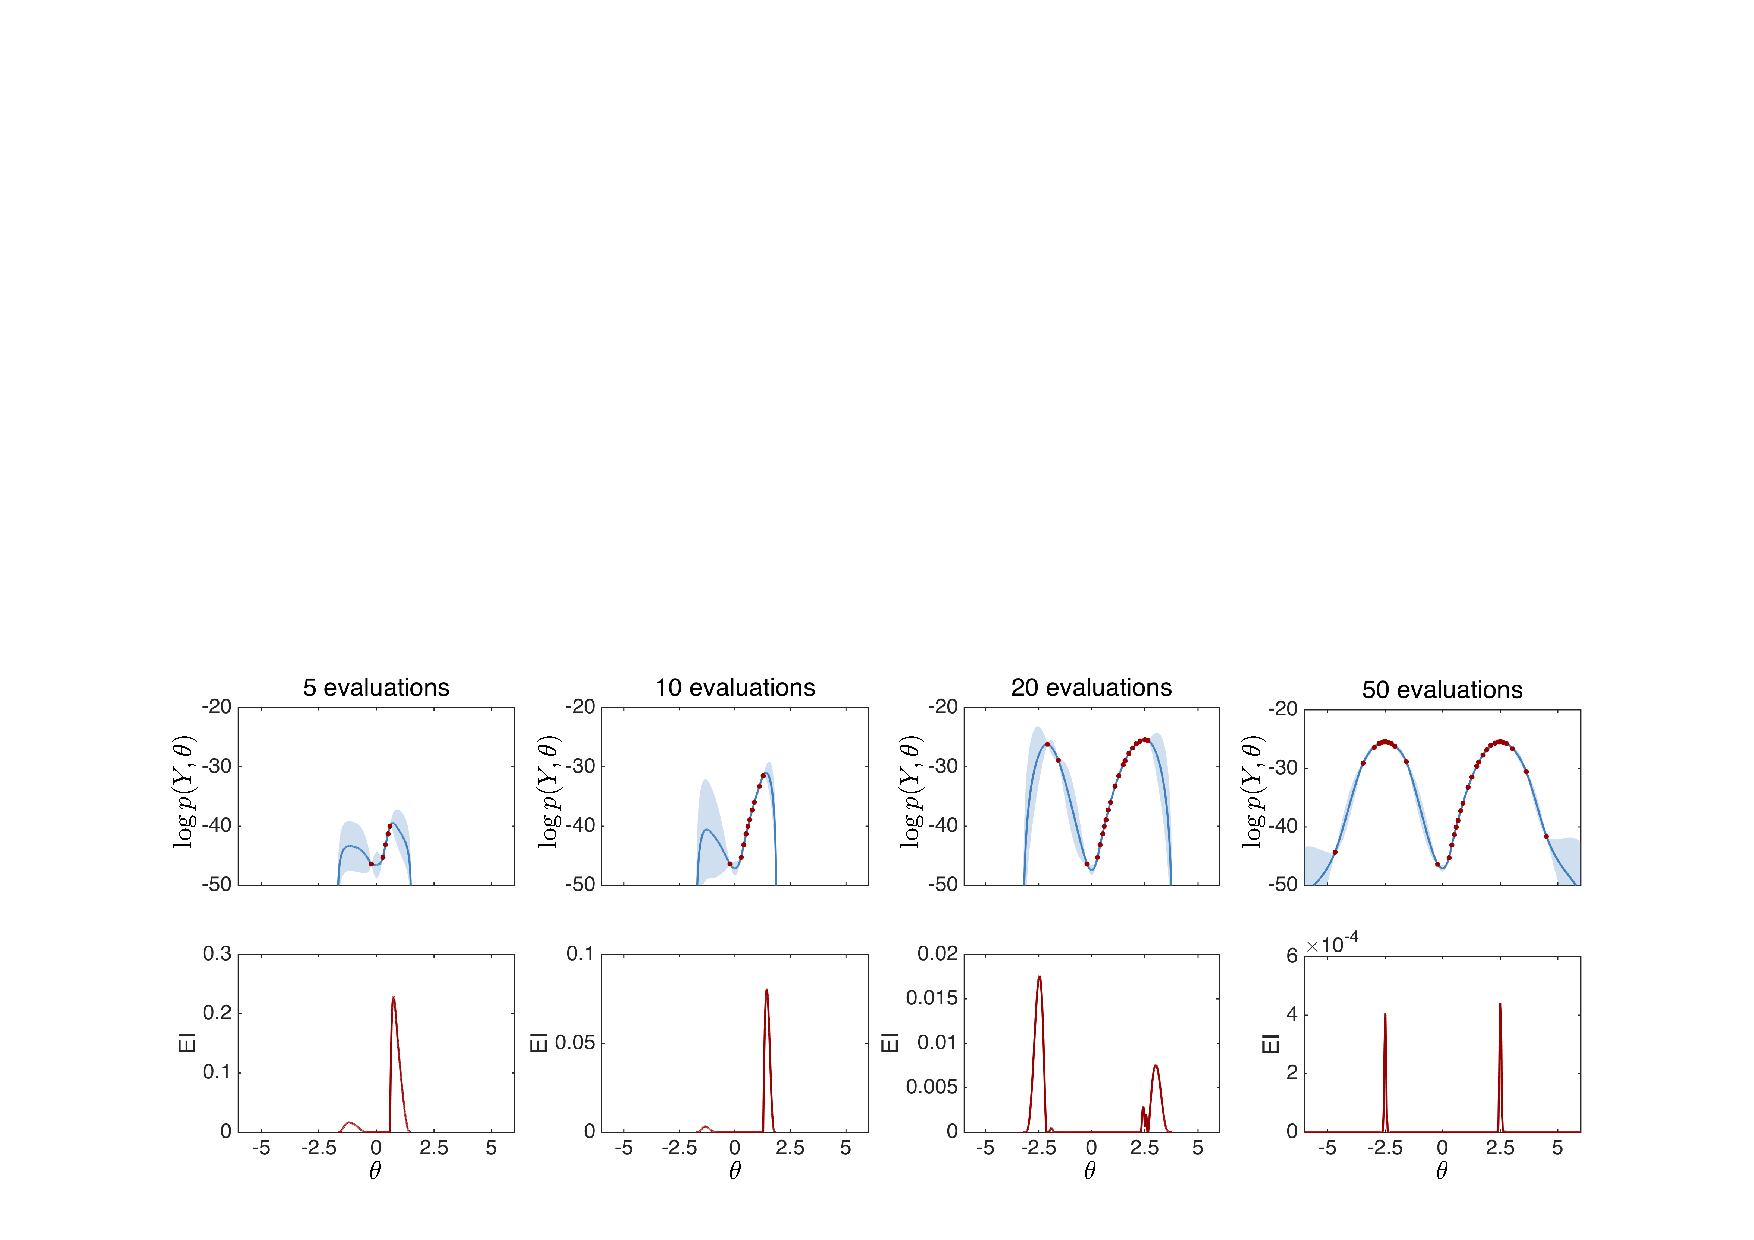
\includegraphics[width=0.99\textwidth]{unbounded_opt}
	\caption{Convergence on an unconstrained bimodal problem with $p \left(\theta\right)={\rm Normal}(0, 0.5)$ and $p \left(Y|\theta\right)={\rm Normal}(5-\left|\theta\right|,0.5)$ giving significant prior misspecification. The top plots show a regressed GP, with the solid line corresponding to the mean and the shading shows $\pm$ 2 standard deviations.  The bottom plots show the corresponding acquisition functions. \label{fig:domainAdpat}}
\end{figure*}

We first demonstrate the ability of BOPP to carry out unbounded optimization using a 1D problem with a significant prior-posterior mismatch as shown in Figure \ref{fig:domainAdpat}.  It shows BOPP adapting to the target and effectively establishing a maxima in the presence of multiple modes.   After 20 evaluations the acquisitions begin to explore the right mode, after 50 both modes have been fully uncovered.

\begin{figure*}[t]
	\centering
	
\includegraphics[width=1\textwidth]{combined_opt_plots}
	%	\includegraphics[width=1.35in]{figures/bayes-opt-comp/branin.pdf}
	%	\includegraphics[width=1.35in]{figures/bayes-opt-comp/hartmann.pdf}
	%	\includegraphics[width=1.35in]{figures/bayes-opt-comp/svm.pdf}
	%	\includegraphics[width=1.35in]{figures/bayes-opt-comp/lda.pdf}
	\caption{Comparison of BOPP  used as an optimizer to prominent BO packages on common benchmark problems.  
		%Branin and Hartmann 6D represent are continuous optimizations, whilst SVM on-grid and LDA on-grid are discrete.  
		The dashed lines shows the final mean error of SMAC (red), Spearmint (green) and TPE (black) as quoted by \cite{eggensperger2013towards}. % which also provides further details on the other packages and the benchmark problems.  
		The dark blue line shows the mean error for BOPP averaged over 100 runs, whilst the median and 25/75\% percentiles are shown in cyan. Results for Spearmint on Branin and SMAC on SVM on-grid are omitted because both BOPP and the respective algorithms averaged zero error to the provided number of significant figures in \cite{eggensperger2013towards}.
		%, meaning it not possible to check where BOPP performed better or worse then the alternative in these two cases.
		\label{fig:bayes-opt}}
\end{figure*}

\subsection{Classic Optimization Benchmarks}

Next we compare BOPP to the prominent BO packages SMAC \cite{hutter2011sequential}, Spearmint \cite{snoek2012practical} and TPE \cite{bergstra2011algorithms} on a number of classical benchmarks as shown in Figure \ref{fig:bayes-opt}.  These results demonstrate that BOPP provides substantial advantages over these systems when used simply as an optimizer on both continuous and discrete optimization problems.  In particular, it offers a large advantage over SMAC and TPE on the continuous problems (Branin and Hartmann), due to using a more powerful surrogate, and over Spearmint on the others due to not needing to make approximations to deal with discrete problems.

\subsection{Marginal Maximum a Posteriori Estimation Problems}

We now demonstrate application of BOPP on a number of MMAP problems.  Comparisons here are more difficult due to the dearth of existing alternatives for PPS.  In particular, simply running inference on the original query does not return estimates for $p\left(Y,\theta\right)$.  We consider the possible alternative of using our conditional code transformation to design a particle marginal Metropolis Hastings (PMMH, \cite{andrieu2010particle}) sampler which operates in a similar fashion to BOPP except that new $\theta$ are chosen using a MH step instead of actively sampling with BO.
%\footnote{To carry out MMAP one could further apply an annealing to the PMMH.  We omit this here as the behaviour of such as system would be indistinguishable from the presented results, due to the small number of iterations and very large variations of $p\left(\theta\right)$ for changes in $\theta$.}
For these MH steps we consider both LMH \citep{wingate2011lightweight} with proposals from the prior and the random-walk MH (RMH) variant introduced in Section~\ref{sec:proginf:str:lmh}.

\subsubsection{Hyperparameter Optimization for Gaussian Mixture Model}

% !TEX root =  bopp.tex


\begin{figure}[t]
	\begin{lstlisting}[basicstyle=\footnotesize\ttfamily]
(defopt mvn-mixture [data mu0 kappa psi] [nu alpha]
 (let [[n d] (shape data)
       alpha (sample (uniform-continuous 0.01 100))
       nu (sample (uniform-continuous (- d 1) 100))
       obs-proc0 (mvn-niw mu0 kappa nu psi)]
       (loop [data data
              obs-procs {}
              mix-proc (dirichlet-discrete 
                          (vec (repeat d alpha)))]
	    (let [y (first data)]
	     (if y
	      (let [z (sample (produce comp-proc))
	            obs-proc (get obs-procs z obs-proc0)
	            obs-dist (produce obs-proc)]
	        (observe obs-dist y)
	        (recur (rest data)
	               (assoc obs-procs z (absorb obs-proc y))
	        (absorb mix-proc z)))
	      mix-proc)))))
	\end{lstlisting}
	\caption{
		\label{fig:mvn-code}
		Anglican query for hyperparameter optimization of a Gaussian mixture model, defined in terms of two parameters \lsi{nu} and \lsi{alpha}. A \lsi{mvn-niw} process is used to represent the marginal likelihood of observations under a Gaussian-inverse-Wishart prior, whereas a \lsi{dirichlet-discrete} process models the prior probability of cluster assignments under a Dirichlet-discrete prior. The command \lsi{produce} returns the predictive distribution for the next sample from a process. \lsi{absorb} conditions on the value of the next sample.}
\end{figure}

\begin{figure*}[t]
	%	\includegraphics[width=1.7in]{"../figures/mvn-mixture/opt-nu-alpha-160229-01-10"}
	%	~
	%	\includegraphics[width=1.7in]{"../figures/mvn-mixture/opt-nu-alpha-160229-01-20"}
	%	~
	%	\includegraphics[width=1.7in]{"../figures/mvn-mixture/opt-nu-alpha-160229-01-50"}
	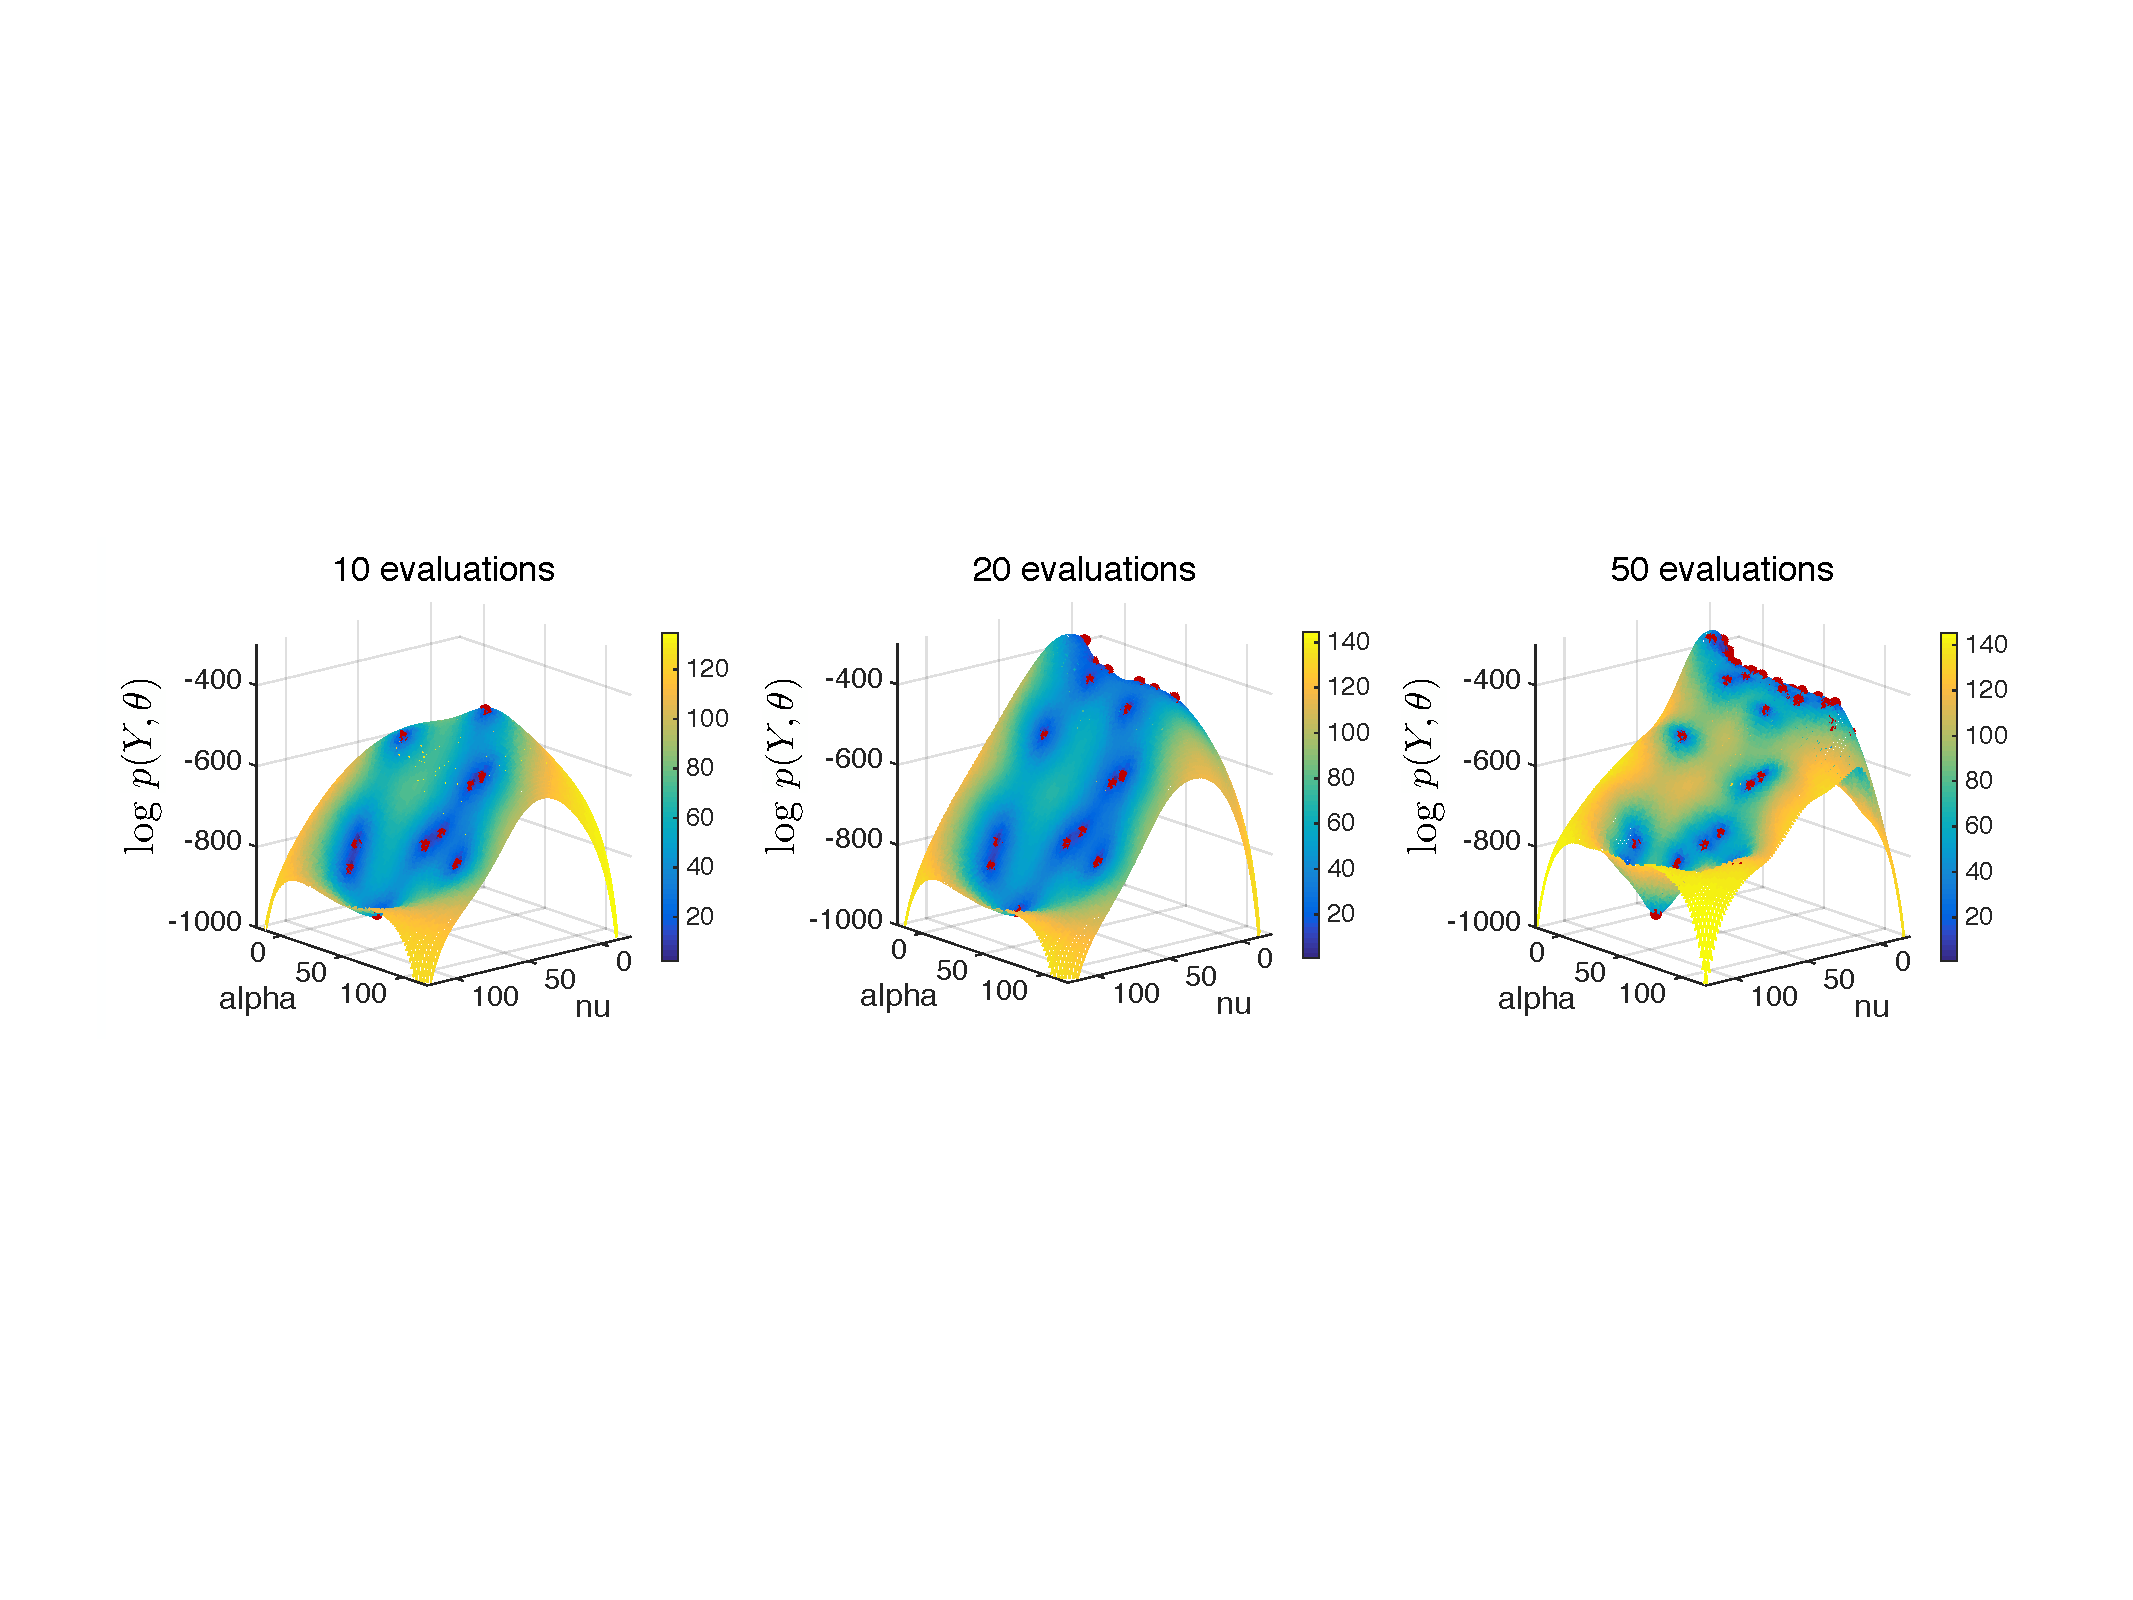
\includegraphics[width=\textwidth]{mvn-mixture/axis_corr_mvn_gps}
	\caption{
		\label{fig:mvn-gp-surface}
		Bayesian optimization of hyperparameters in a Gaussian mixture model evaluated on the Iris dataset. Panels show the GP posterior as a function of number of evaluations, with the surface corresponding to the posterior mean and the color bars the posterior standard deviation. Optimization is performed over the parameter $\alpha$ of a 10-dimensional symmetric Dirichlet distribution and the degrees of freedom $\nu$ of the inverse-Wishart prior. At each evaluation we obtain an estimate of the log marginal $\log p(Y,\theta)$ obtained by performing sequential Monte Carlo inference with 1000 particles.  The apparent maximum after initialization with 10 randomly sampled points lies at $\nu=31$, $\alpha=60$, and $\log p(Y,\theta) = -456.3$ (\emph{left}).  The surface after 10 optimization steps shows a new maximum at $\nu=9.2$, $\alpha=0.8$, and $\log p(Y,\theta) = -364.2$ (\emph{middle}). After 40 steps and 50 total evaluations this optimum is refined to $\nu=16$, $\alpha = 0.2$, and $\log p(Y,\theta) = -352.5$  (\emph{right}).}
\end{figure*}

We start with an illustrative case study of optimizing the hyperparameters in a multivariate Gaussian mixture model. We consider a Bayesian formulation with a symmetric Dirichlet prior on the mixture weights and a Gaussian-inverse-Wishart prior on the likelihood parameters:
\begin{align}
\v{\pi}
&\sim 
{\rm Dir(\alpha, \ldots, \alpha)}
\displaybreak[0]\\
(\v{\mu}_k, \v{\Sigma}_k)
&\sim 
{\rm NIW} (\v{\mu}_0, \kappa, \v{\Psi}, \nu)
&
{\rm for~}
&
k = 1, \ldots , K
\displaybreak[0]\\
z_n 
&\sim 
{\rm Disc(\v{\pi})}
\displaybreak[0]\\
\v{y}_n
&
\sim
{\rm Norm}(\v{\mu}_{z_n}, \v{\Sigma}_{z_n})
&
{\rm for~}
&
n = 1, \ldots , N
\end{align}
% Figure~\ref{fig:mvn-code} shows an optimization query for an Anglican program corresponding to this model. 
Anglican code for this model is shown in Figure 4. Anglican provides stateful objects, which are referred to as random processes, to represent the predictive distributions for the cluster assignments $z$ and the observations $\v{y}^k$ assigned to each cluster
\begin{align}
z_{n+1}
& \sim 
p( \cdot \,|\, z_{1:n}, \alpha),
\\
\v{y}_{m+1}^{k} 
& \sim 
p(\cdot \,|\, \v{y}^k_{1:m}, \v{\mu}_0, \kappa, \v{\Psi}, \nu).
\end{align}
In this collapsed representation marginalization over the model parameters $\v{\pi}$, $\v{\mu}_{k=1:K}$, and $\v{\Sigma}_{k=1:K}$ is performed analytically.
%The only variables that are sampled during program execution are the cluster assignments $z_{1:N}$, which we marginalize over using the general-purpose sequential Monte Carlo (SMC) implementation provided by the inference back end. 
%Like any importance sampling method, SMC provides an unbiased estimate $\hat Z$ of the marginal likelihood $Z = p(\v{y}_{1:N} | \alpha, \v{\mu}, \kappa, \v{\Psi}, \nu)$. 
%Intuitively, the parameter $\nu$, which is known as the degrees of freedom, represents a scale factor for the covariance matrix, which determines the spatial extent of the clusters (larger $\nu$ values imply a smaller covariance and cluster size). 
%The parameter $\alpha$, sometimes known as a concentration parameter, controls the distribution on mixture weights (where $\alpha \gg 1.0$ implies an even distribution and $\alpha \ll 1.0$ implies an uneven distribution).  
Using the Iris dataset, a standard benchmark for mixture models that contains 150 labeled examples with 4 real-valued features, we optimize the marginal with respect to the subset of the parameters $\nu$ and $\alpha$ under uniform priors over a fixed interval.  For this model, BOPP aims to maximize
\begin{align}
\begin{split}
& p(\nu, \alpha | \v{y}_{n=1:N}, \v{\mu}_0, \kappa, \v{\Psi}) \\
&= \iiiint p(\nu, \alpha, z_{n=1:N}, \v{\pi}, \v{\mu}_{k=1:K}, \v{\Sigma}_{k=1:K} | \v{y}_{n=1:N}, \mu_0, \kappa, \v{\Psi}) \mathrm{d}z_{n=1:N}\mathrm{d}\v{\pi}\mathrm{d}\v{\mu}_{k=1:K}\mathrm{d}\v{\Sigma}_{k=1:K}.
\end{split}
\end{align}

Figure~\ref{fig:mvn-gp-surface} shows GP regressions on the evidence after different numbers of the SMC evaluations have been performed on the model.  This demonstrates how the GP surrogate used by BO builds up a model of the target, used to both estimate the expected value of $\log p(Y,\theta)$ for a particular $\theta$ and actively sample the $\theta$ at which to undertake inference.

% n=10
% x1_max: 30.90
% x2_max: 61.55
% y_max: -456.32
% mu_max: -456.33
% sig_max: 0.51

% n=20
% x1_max: 9.20
% x2_max: 0.79
% y_max: -364.21
% mu_max: -364.23
% sig_max: 0.47

% n=50
% x1_max: 16.34
% x2_max: 0.21
% y_max: -352.51
% mu_max: -352.51
% sig_max: 0.53

% n=100
% x1_max: 16.34
% x2_max: 0.21
% y_max: -352.51
% mu_max: -352.50
% sig_max: 0.41

% \begin{figure}
% \begin{lstlisting}[basicstyle=\footnotesize\ttfamily]
% (defopt mvn-mixture 
%  [data mu kappa psi] [:nu :alpha]
%  (let [[n d] (shape data)
%        alpha (sample :alpha
%               (uniform-continuous 0.01 100))
%        nu (sample :nu 
%            (uniform-continuous (- d 1) 100))
%        obs-proc0 (mvn-niw mu kappa nu psi)]
%   (loop [data data
%          obs-procs {}
%          mix-proc (dirichlet-discrete 
%                    (vec (repeat d alpha)))]
%    (let [y (first data)]
%     (if y
%      (let [z (sample (produce comp-proc))
%            obs-proc (get obs-procs 
%                      z obs-proc0)
%            obs-dist (produce obs-proc)]
%       (observe obs-dist y)
%       (recur (rest data)
%              (assoc obs-procs
%                z (absorb obs-proc y))
%              (absorb mix-proc z)))
%      (predict mix-proc))))))
% \end{lstlisting}
% \caption{
% \label{fig:mvn-code}
% Anglican query for hyperparameter optimization of a Gaussian mixture model, defined in terms of two parameters \lsi{:nu} and \lsi{:alpha}. A \lsi{mvn-niw} process is used to represent the marginal likelihood of observations under a Gaussian-inverse-Wishart prior, whereas a \lsi{dirichlet-discrete} process models the prior probability of cluster assignments under a Dirichlet-discrete prior. The command \lsi{produce} returns the predictive distribution for the next sample from a process. \lsi{absorb} conditions on the value of the next sample.}
% \end{figure}





% 


\subsubsection{Extended Kalman Filter for the Pickover Chaotic Attractor}
\label{sec:AppKalman}

% !TEX root =  ../main.tex


\begin{figure*}[t]
	\centering
	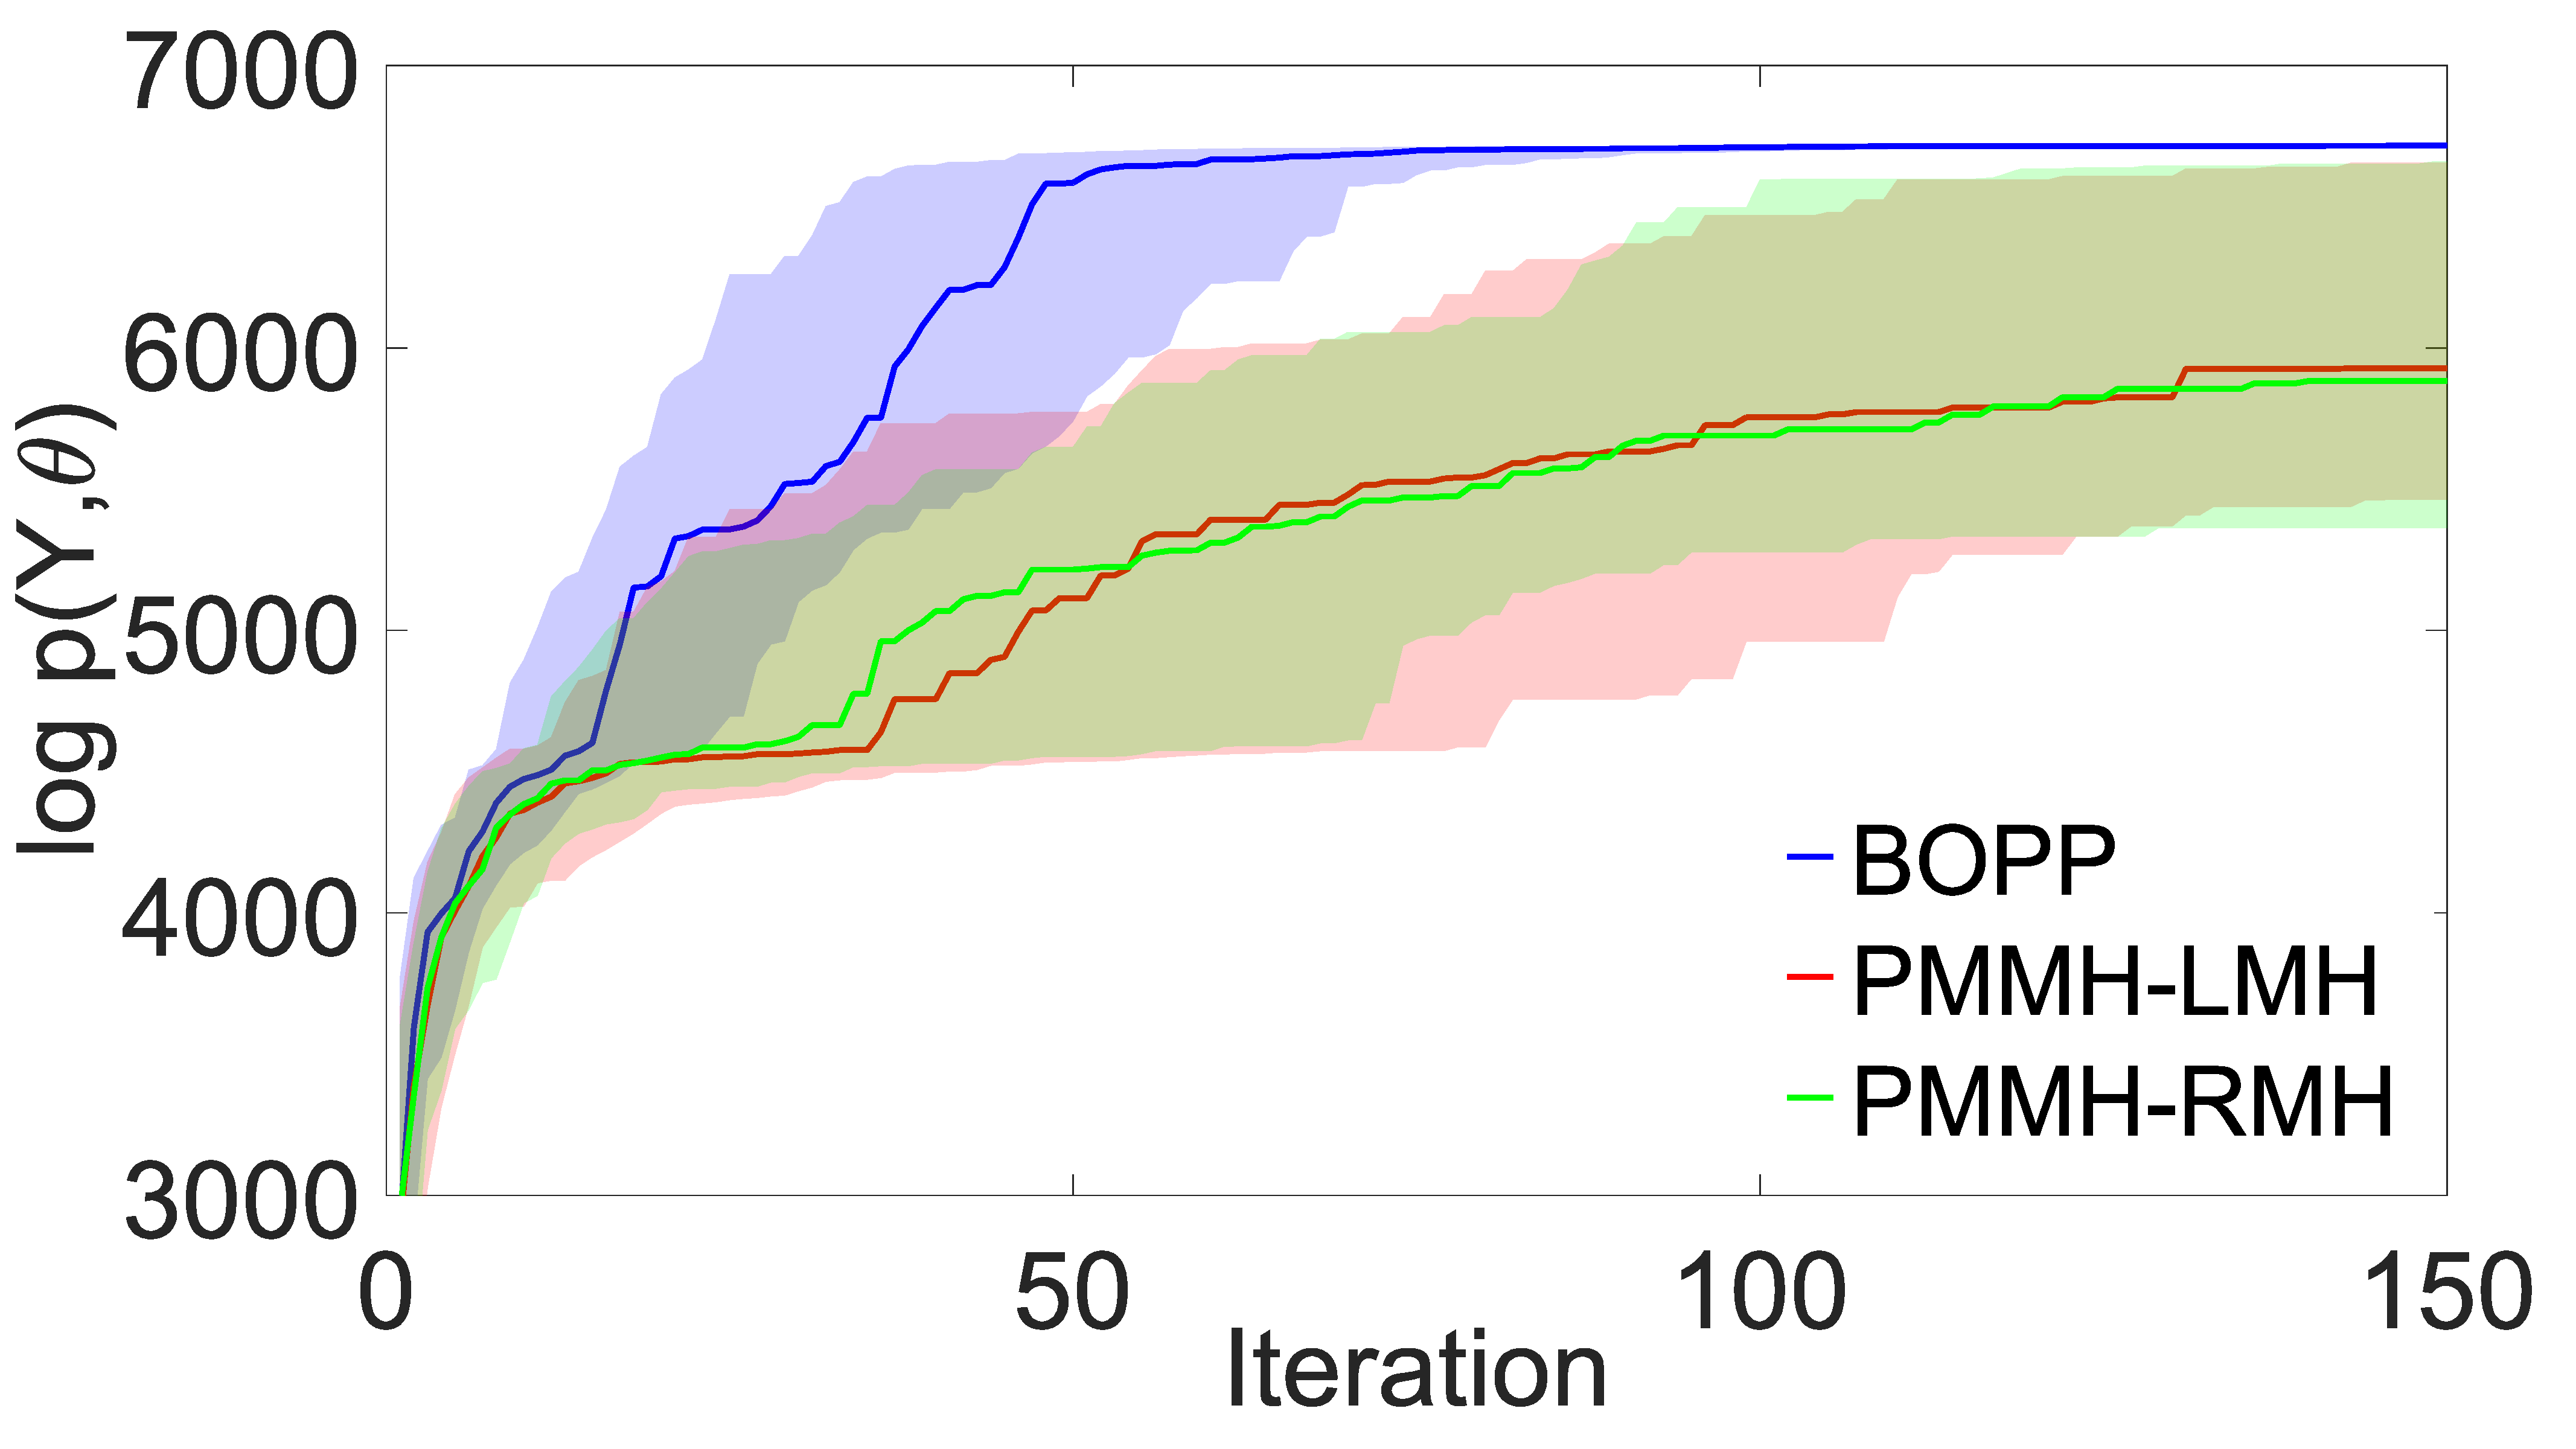
\includegraphics[width=2.72in]{chaos/chaos_ml.pdf}
	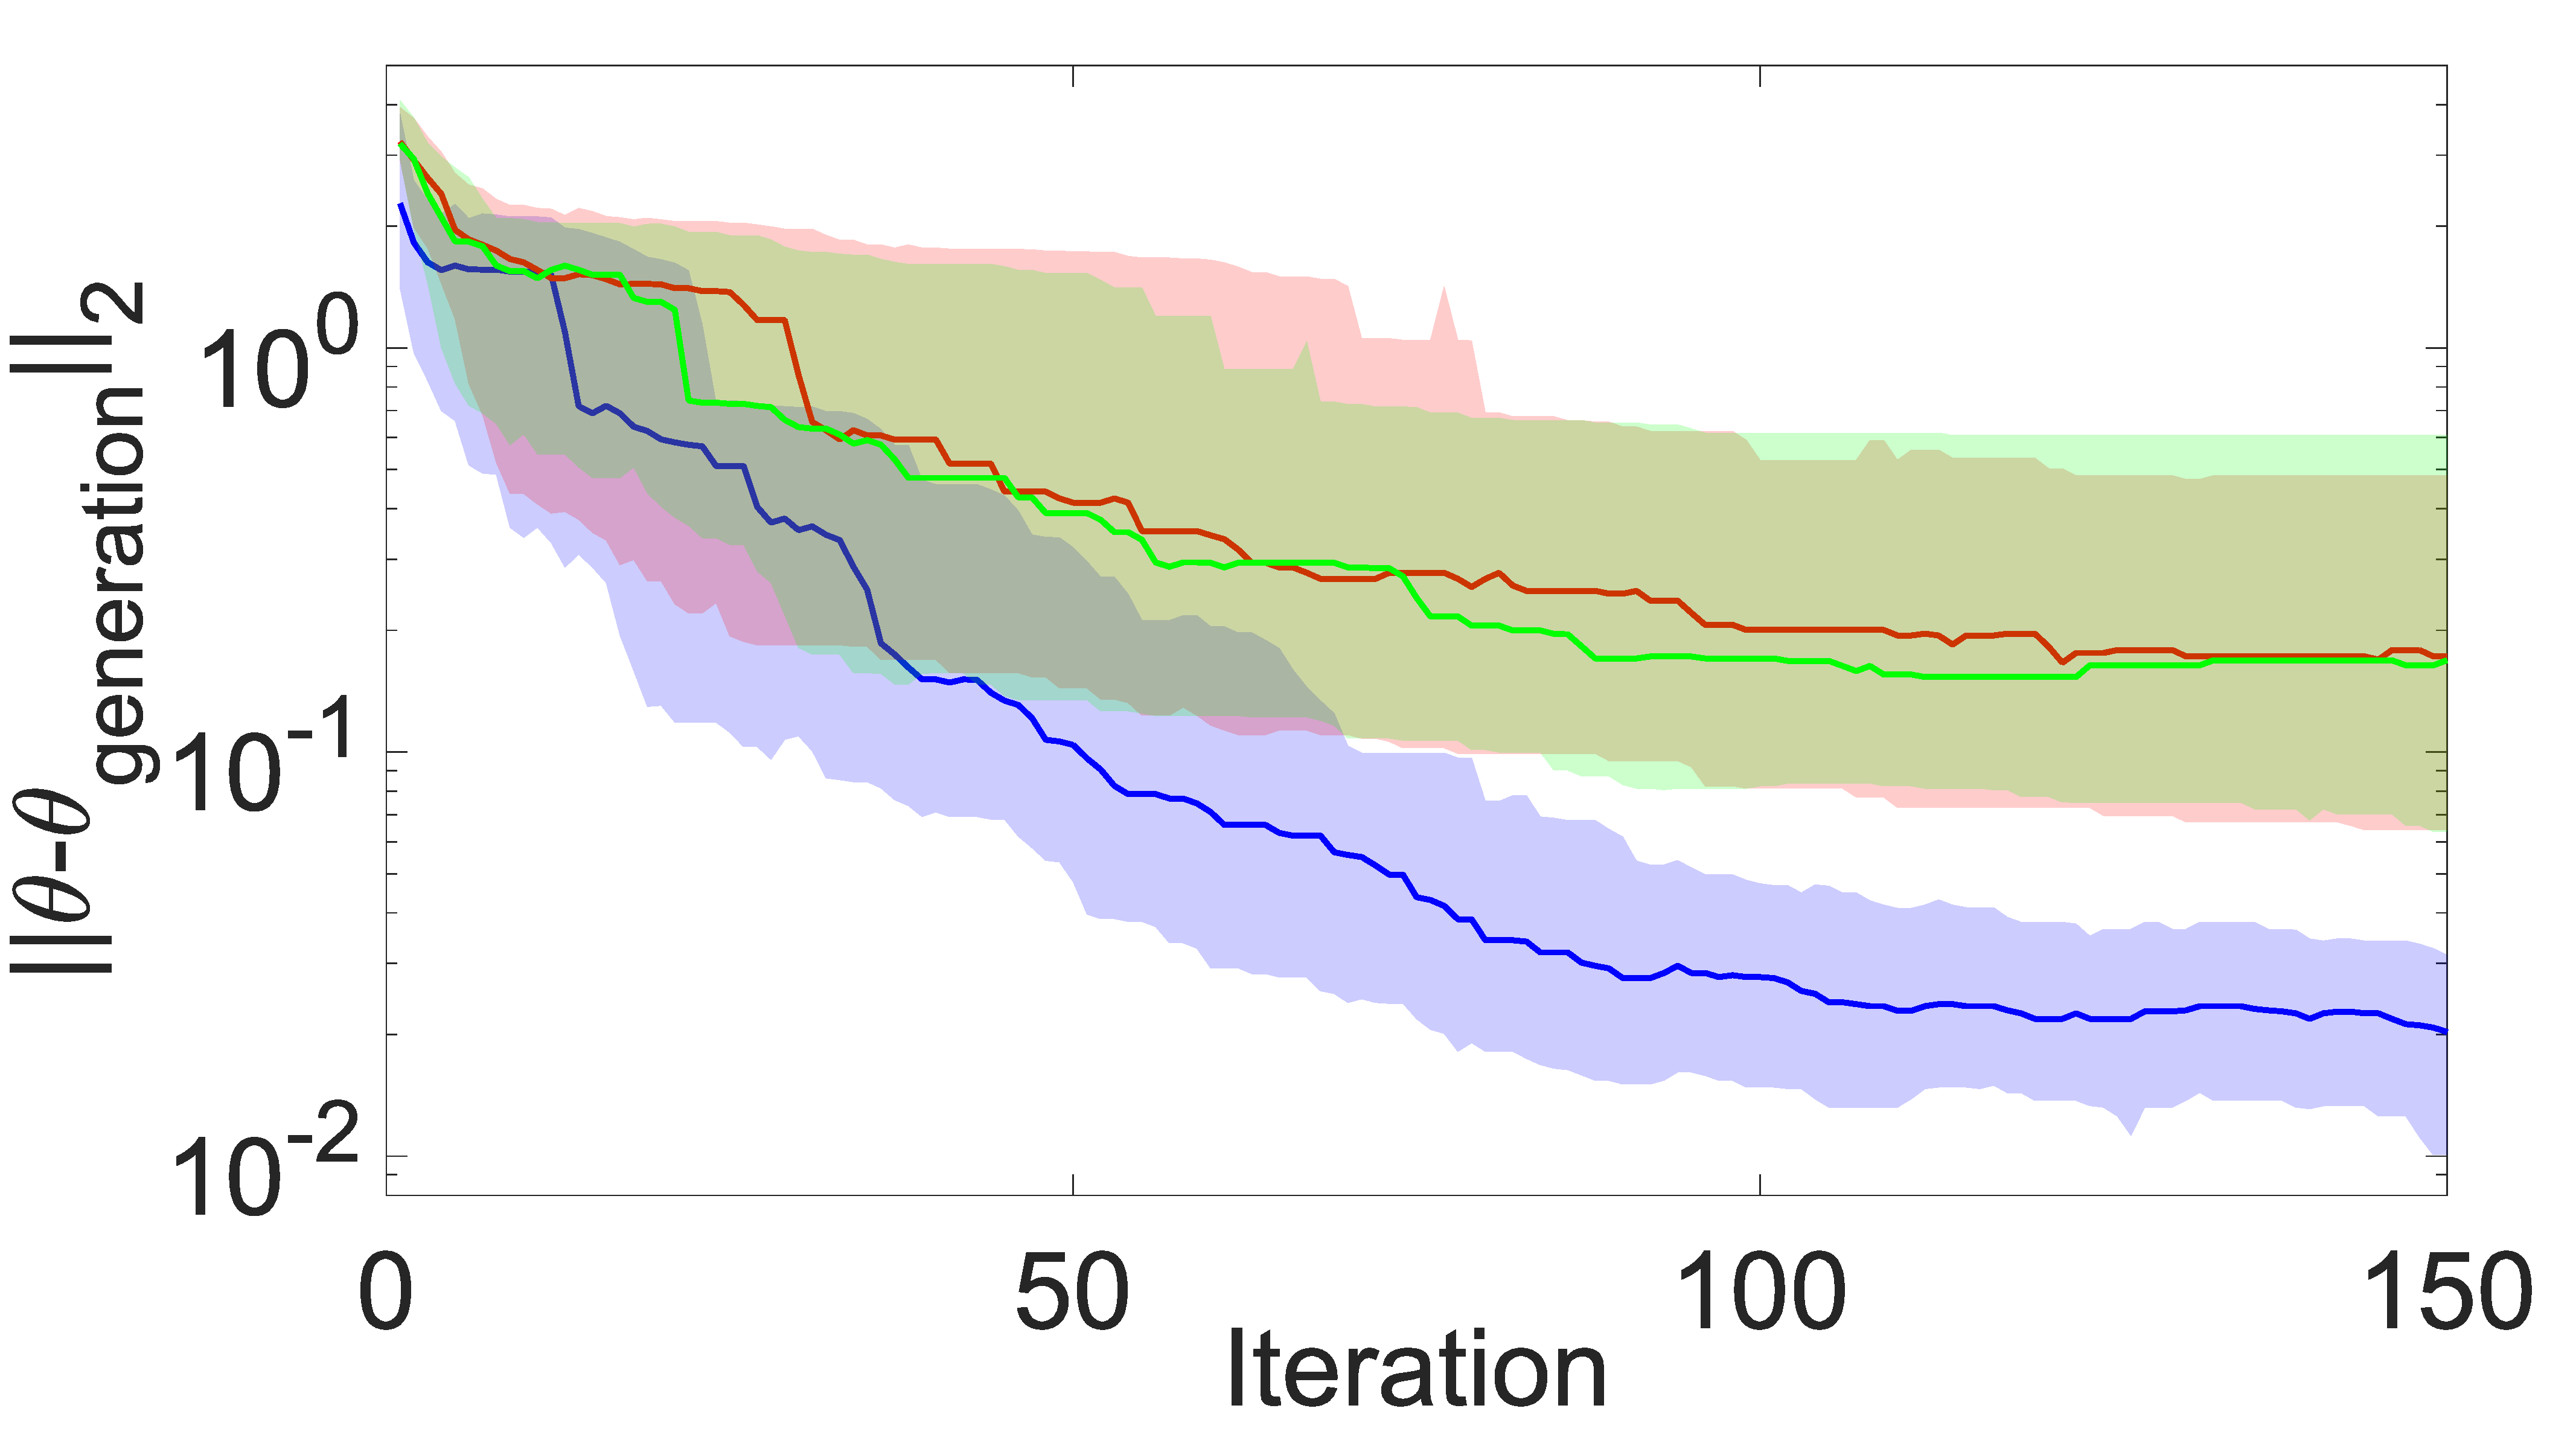
\includegraphics[width=2.72in]{chaos/chaos_distance.pdf}
	\caption{Convergence for transition dynamics parameters of the pickover attractor in terms of the cumulative best $\log p\left(Y,\theta\right)$ (\emph{left}) and distance to the ``true" $\theta$ used in generating the data (\emph{right}). Solid line shows median over 100 runs, whilst the shaded region the 25/75\% quantiles.  \label{fig:chaos}
		\vspace{6pt}}
\end{figure*}

\begin{figure}[t]
	\centering
	\begin{subfigure}[t]{0.24\textwidth}
		\centering
		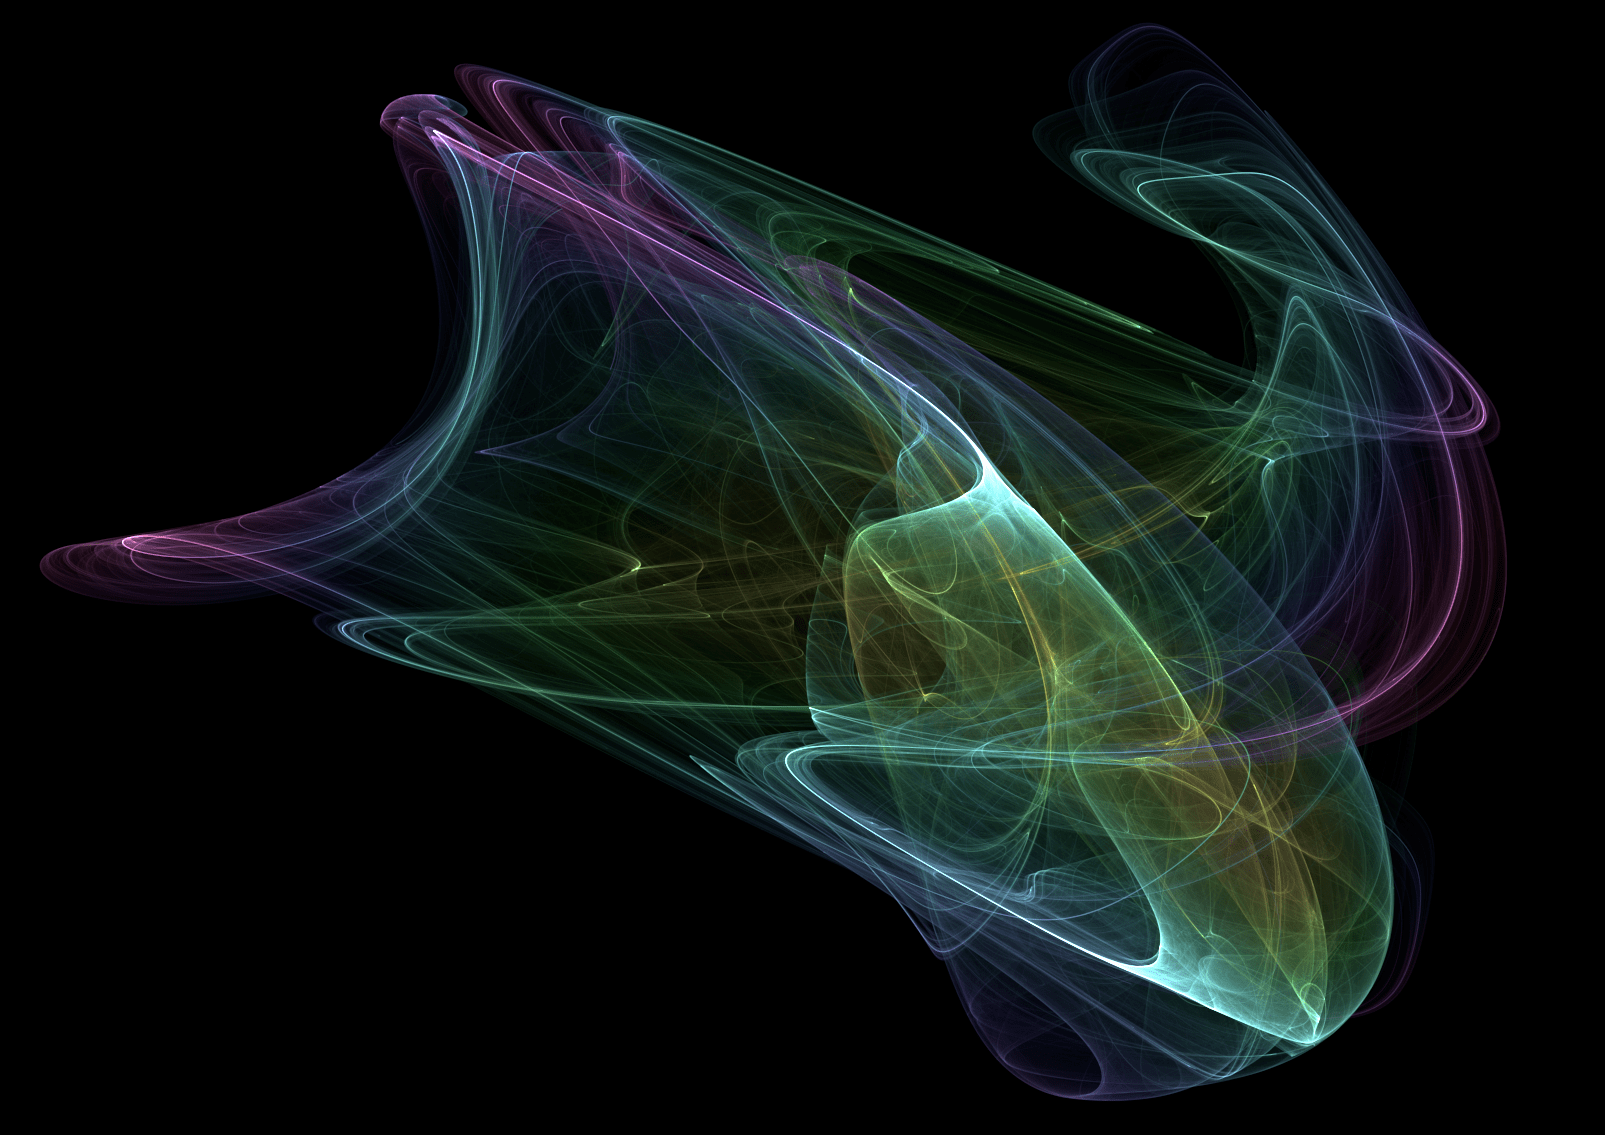
\includegraphics[height=3.2cm,width=3.7cm]{chaos/compressed/first_iter_alt.png}
		\caption{1 iteration}
	\end{subfigure}
	\begin{subfigure}[t]{0.24\textwidth}
		\centering
		\tiny
		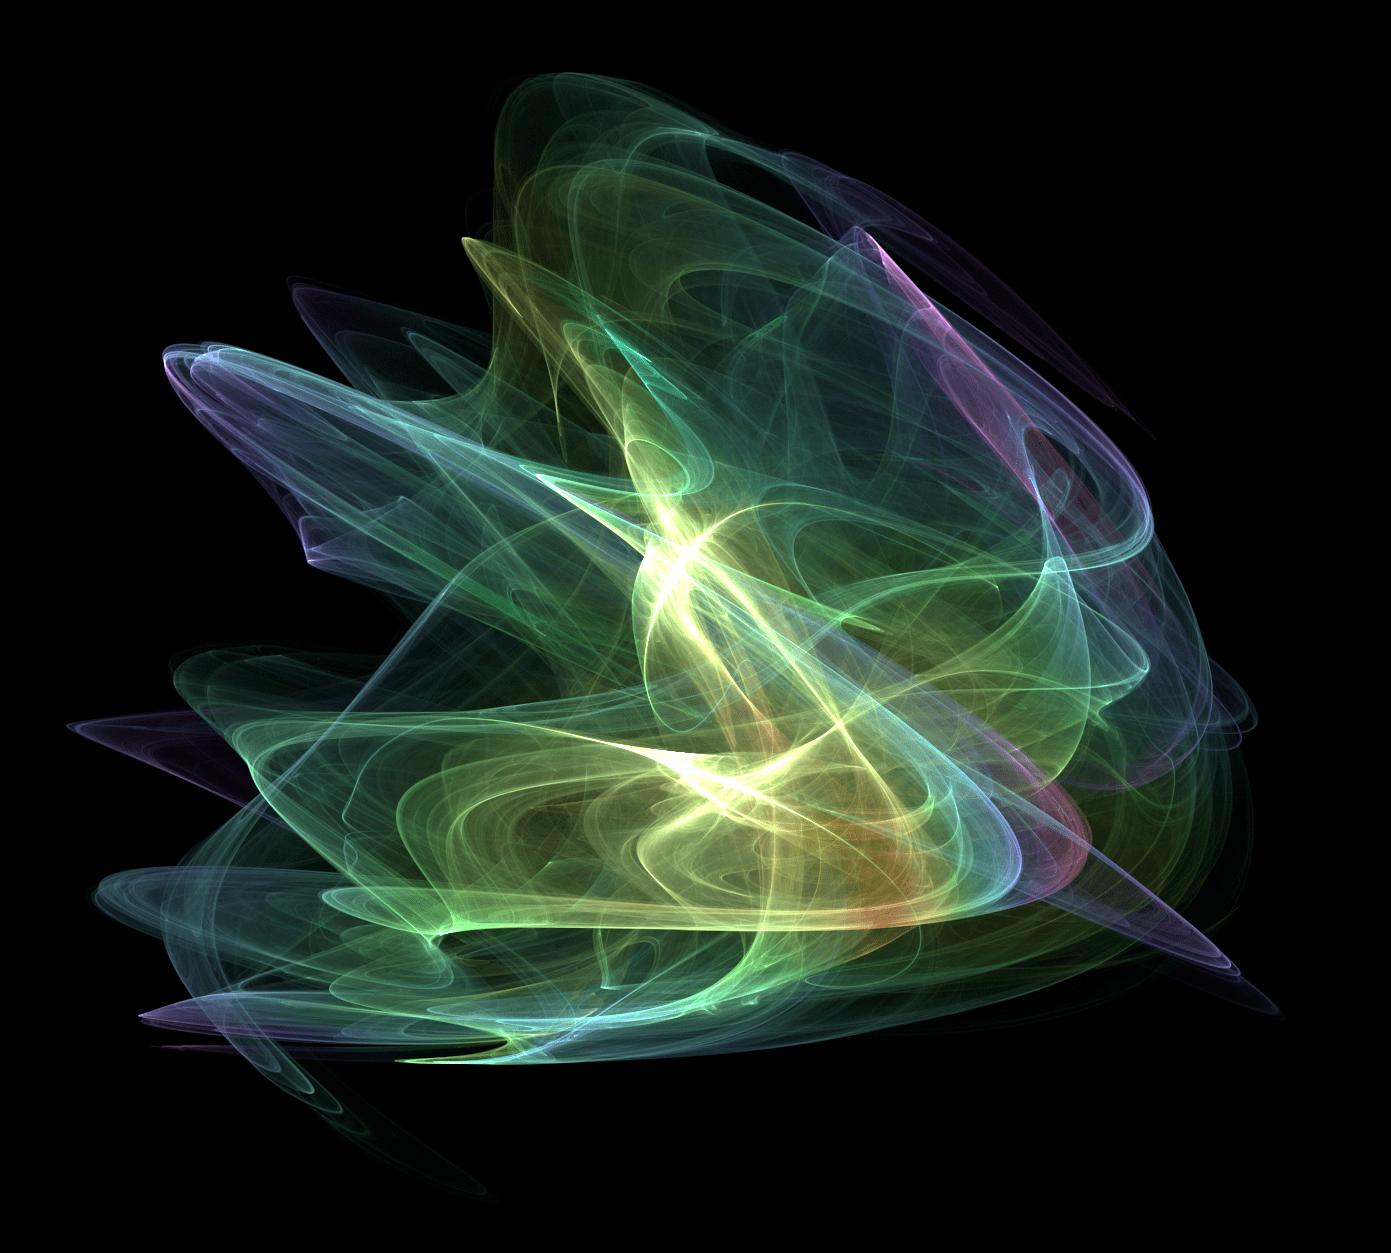
\includegraphics[height=3.2cm,width=3.7cm]{chaos/compressed/20_iter_alt.png}
		\caption{20 iterations}
	\end{subfigure}
	\begin{subfigure}[t]{0.24\textwidth}
		\centering
		\tiny
		
\includegraphics[height=3.2cm,width=3.7cm]{chaos/compressed/100_iter_altj.png}
		\caption{100 iterations}
	\end{subfigure}
	\begin{subfigure}[t]{0.24\textwidth}
		\centering
		\tiny
		\includegraphics[height=3.2cm,width=3.7cm]{chaos/compressed/target_light.png}
		\caption{Ground truth}
	\end{subfigure}
	\caption{A series of trajectories for different parameters, demonstrating convergence to the true attractor.  The colormap is based on the speed and curvature of the trajectory, with rendering done using the program Chaoscope (available at {\href{http://www.chaoscope.org/}{http://www.chaoscope.org/}}). \label{fig:chaoscope}}
\end{figure}

Our first MMAP example considers the case of learning the dynamics parameters of a chaotic attractor.  
This constitutes a class Markovian state space model problem, specifically a Kalman smoother,
where we observe a noisy signal 
$y_t \in \real^{K}, \; t = 1,2,\dots,T$ in some $K$ dimensional observation space were each 
observation has a lower dimensional latent parameter $x_t \in \real^{D},  \; t = 1,2,\dots,T$.
In addition to an initial distribution $x_1 \sim \mathcal{N} \left(\mu_1, \sigma_1 I\right)$, our model is specified by 
\begin{subequations}
	\label{eq:Kalman}
\begin{align}
x_t = & A \left(x_{t-1}, \theta\right)+\delta_{t-1}, \; & \delta_{t-1} \sim \mathcal{N} \left(0, \sigma_q I\right) \\
y_t = & C x_{t}+\varepsilon_{t}, \; & \varepsilon_{t} \sim \mathcal{N} \left(0, \sigma_y I\right)
\end{align}
\end{subequations}
where $I$ is the identity matrix, $C$ is a known $K \times D$ matrix, and $\mu_1,\sigma_1, \sigma_q$ 
and $\sigma_y$ are all known scalars.  Our aim is to learn the dynamics parameters $\theta$ given
$y_{1:T}$, marginalizing over the latent variables $x_{1:T}$.  We use
a uniform prior on the parameters $\theta$, which means that the MMAP values for $\theta$
coincide with their (constrained) MML values.  A synthetic dataset was generated with $T=500$ and
$K=20$ (see \cite{rainforth2017boppArxiv}).
Inference on \qmarg was carried out using SMC with 500 particles.  
Convergence results are given in Figure~\ref{fig:chaos} showing that BOPP comfortably 
outperforms the PMMH variants, while Figure~\ref{fig:chaoscope} shows the simulated 
attractors generated from the dynamics parameters output by various iterations of a 
particular run of BOPP.


\subsubsection{Hidden Markov Model with Unknown Number of States}

% !TEX root =  ../main.tex

\begin{figure*}[t]
	\centering
	\includegraphics[width=2.72in]{hmm/hmm_ML}
	~~~~~~
	\includegraphics[width=2.72in]{hmm/hmm_distance}
	\caption{Convergence for HMM in terms of the cumulative best $\log p\left(Y,\theta\right)$ (\emph{left}) and distance to the ``true" $\theta$ used in generating the data (\emph{right}). Solid line shows median over 100 runs, whilst the shaded region the 25/75\% quantiles.  Note that for the distance to true $\theta$ was calculated by selecting the three states (out of the 5 generated) that were closest to the true parameters.  \label{fig:hmm}}
\end{figure*}

We finish by considering a hidden Markov model (HMM) with an unknown number of discrete possible states.  
This example demonstrates how BOPP can still be applied to models which conceptually have an 
unknown number of target variables, by generating all possible variables that might be needed, 
but then leaving some variables unused for some execution traces.  This avoids problems 
of varying reference measures so that the MMAP problem is well defined  and provides a 
function with a fixed number of inputs as required by the BO scheme.  From the BO 
perspective, the target function is simply constant for variations in an unused variable.

Our model places a uniform prior on the number of states $K \sim \textsc{Discrete}\{1,2,3,4,5\}$.
Each emission distribution corresponds to a Gaussian with unknown mean (which we wish to
optimize) and known variance.  
We marginalize over are the transition distribution parameters and the HMM latent states.  
Rather than constructing a model were the emission distribution
parameters only exist conditioned on the value of $K$, we generate variables for all $5$ emission
distributions that might be required, with only the first $K$ actually then used.  
A synthetic dataset was generated using $K=3$ and $T=1000$ observations.  Results of running BOPP are given
in Figure~\ref{fig:hmm}, again showing that BOPP outperforms these PMMH alternatives.  See~\cite{rainforth2017boppArxiv}
for further details.


%
%\subsection{Full Details for House Heating Experiment}
%\label{sec:app:heating}
%
%% !TEX root =  bopp.tex

In this case study, illustrated in Figure~\ref{fig:houses}, we optimize the parameters of a stochastic engineering simulation. We use the Energy2D system from \cite{xie2012energy2d} to perform finite-difference numerical simulation of the heat equation and Navier-Stokes equations in a user-defined geometry. 

In our setup, we designed a 2-dimensional representation of a house with 4 interconnected rooms using the GUI provided by Energy2D. The left side of the house receives morning sun, modelled at a constant incident angle of $30^\circ$. We assume a randomly distributed solar intensity and simulate the heating of a cold house in the morning by 4 radiators, one in each of the rooms. The radiators are given a fixed budget of total power density $P_{\text{budget}}$. The optimization problem is to distribute this power budget across radiators in a manner that minimizes the variance in temperatures across 8 locations in the house. 

Energy2D is written in Java, which allows the simulation to be integrated directly into an Anglican program that defines a prior on model parameters and an ABC likelihood for evaluating the utility of the simulation outputs. Figure \ref{fig:house-heating-code} shows the corresponding program query. In this, we define a Clojure function \lsi{simulate} that accepts a solar power intensity $I_{\text{sun}}$ and power densities for the radiators $P_{\text{r}}$, returning the thermometer temperature readings $\{T_{i, t}\}$. We place a symmetric Dirichlet prior on $\frac{P_r}{P_{\text{budget}}}$ and a gamma prior on $\frac{I_{\text{sun}}}{I_{base}}$, where $P_{\text{budget}}$ and $I_{base}$ are constants. This gives the generative model:
 \begin{align}
 p_r &\sim \Dirichlet([1,1,1,1]) \\
 P_r &\leftarrow P_{\text{budget}} \cdot p_r \\
 \upsilon &\sim \text{Gamma}(5,1) \\
 I_{\text{sun}} &\leftarrow I_{\text{base}} \cdot \upsilon.
 \end{align}
After using these to call \lsi{simulate}, the standard deviations of the returned temperatures is calculated for each time point,
\begin{align}
\omega_t = \sqrt{\sum_{i=1}^8 T_{i, t}^2 -\left(\sum_{i=1}^8 T_{i, t}\right)^2}
\end{align}
and used in the ABC likelihood \lsi{abc-likelihood} to weight the execution trace using a multivariate Gaussian:
\begin{align*}
p\left(\{T_{i, t}\}_{i = 1:8, t = 1:\tau}\right) = \text{Normal}\left(\omega_{t=1:\tau};\mathbf{0},\sigma_T^{2}\mathbf{I}\right)
\end{align*}
where $\mathbf{I}$ is the identity matrix and $\sigma_T = 0.8 ^{\circ} \mathrm{C}$ is the observation standard deviation.

Figure \ref{fig:houses} demonstrates the improvement in homogeneity of temperatures as a function of total number of simulation evaluations. Visual inspection of the heat distributions also shown in Figure \ref{fig:houses} confirms this result, which serves as an exemplar of how BOPP can be used to estimate marginally optimal simulation parameters.


\section{Discussion}
\label{sec:disc}

% !TEX root =  bopp.tex

We have introduced a new method for carrying out MMAP estimation of probabilistic program variables using Bayesian optimization, representing the first unified framework for optimization and inference of probabilistic programs.  By using a series of code transformations, our method allows an arbitrary program to be optimized with respect to a defined subset of its variables, whilst marginalizing out the rest.  To carry out the required optimization, we introduce a new GP-based BO package that exploits the availability of the target source code to provide a number of novel features, such as automatic domain scaling and constraint satisfaction.  

The concepts we introduce lead directly to a number of extensions of interest, including but not restricted to smart initialization of inference algorithms, adaptive proposals, and nested optimization.  Further work might consider maximum marginal likelihood estimation and risk minimization.  Though only requiring minor algorithmic changes, these cases require distinct theoretical considerations.
%Another interesting possible extension would be to to apply Bayesian quadrature \cite{osborne2012active} to probabilistic programs.

%Although our implementation is currently restricted to optimize numerical variables of fixed dimensionality, it is possible to extend to a more general case using appropriate kernels, such as the arc kernels introduced by \cite{swersky2014raiders}, which cater to scenarios where certain variables may only exist conditioned on the values of other variables.

%\section{Program Transformations in Detail}
%\label{sec:program-transformations}
%% !TEX root = ../main.tex

In this section we give a more detailed and language specific description of our program transformations, code for which can be found at \href{http://www.github.com/probprog/bopp}{\url{http://www.github.com/probprog/bopp}}. %We will refer to the code in explaining the implementation of program transformations for BOPP.

\subsection{Anglican}
Anglican is a probabilistic programming language integrated into Clojure (a dialect of Lisp) and inherits most of the corresponding syntax. Anglican extends Clojure with the special forms \sample and \observe \citep{tolpin2015probabilistic}.  
Each random draw in an Anglican program corresponds to a \sample  call, which can be thought of as a term in the prior. 
Each \observe statement applies weighting to a program trace and thus constitutes a term in the likelihood.
Compilation of an Anglican program, performed by the macro \lsi{query}, corresponds to transforming the code into a variant of continuation-passing style (CPS) code, which results in a function that can be executed using a particular inference algorithm.

Anglican program code is represented by a nested list of expressions, symbols, non-literals for contructing data structures (e.g. \lsi{[...]} for vectors), and command dependent literals (e.g. \lsi{[...]} as a second argument of a \lsi{let} statement which is used for binding pairs).  In order to perform program transformations, we can recursively traverse this nested list which can be thought of as an abstract syntax tree of the program.

Our program transformations also make use of the Anglican forms \lsi{store} and \lsi{retrieve}.  These allow storing any variable in the probabilistic program's execution trace in a state which is passed around during execution and from which we can retrieve these stored values.  The core use for this is to allow the outer query to return variables which are only locally scoped.

To allow for the early termination that will be introduced in Section \ref{sec:bopp-supp/early-term}, it was necessary to add a mechanism for non-local returns to Anglican.  Clojure supports non-local returns only through Java exception handling, via the keywords {\bf\ttfamily\color{cyan} try}~{\bf\ttfamily\color{cyan}throw},~{\bf\ttfamily\color{cyan}catch} and {\bf\ttfamily\color{cyan}finally}.  Unfortunately, these are not currently supported by Anglican and their behaviour is far from ideal for our purposes.  In particular, for programs containing nested {\bf\ttfamily\color{cyan}try} statements, throwing to a particular {\bf\ttfamily\color{cyan}try} in the stack, as opposed to the most recently invoked, is cumbersome and error prone.
%
%Firstly, return values are stored within exceptions which is cumbersome and can cause issues in debugging.  Secondly, it is difficult to control the point of return.  For example, imagine we wish to return from the query itself and so wrap the original query in a {\bf\ttfamily\color{cyan}try-catch} block.  Na\"{i}vely throwing might now cause us to return to an unexpected point if the original query already contained a {\bf\ttfamily\color{cyan}try-catch} block.  Thus controlling the exact return point would require a careful and error-prone mechanism based on custom exception types and catches.

We have instead, therefore, added to Anglican a non-local return mechanism based on the Common Lisp control form \lsi{catch/throw}.  This uses a \emph{catch tag} to link each \lsi{throw} to a particular \lsi{catch}.  For example
\begin{lstlisting}[basicstyle=\footnotesize\ttfamily]
(catch :tag
  (when (> a 0)
    (throw :tag a))
  0)
\end{lstlisting}
is equivalent to \lsi{(max a 0)}.  More precisely, \lsi{throw} has syntax \lsi{(throw tag value)} and will cause the \lsi{catch} block with the corresponding \lsi{tag} to exit, returning \lsi{value}.   If a \lsi{throw} goes uncaught, i.e. it is not contained within a \lsi{catch} block with a matching tag, a custom Clojure exception is thrown.

%To allow for the early termination discussed in Section \ref{sec:bopp-supp/early-term}, it was necessary to add one new primitive to Anglican, namely \lsi{return} with syntax \lsi{(return return-val)}.  At a high level, \lsi{return} causes the query to terminate, returning \lsi{return-val}.  This is done by, during runtime of the CPS compiled code, returning a Clojure record \lsi{->result} containing \lsi{return-val} instead of a valid program continuation, causing the query execution to terminate and return the required value.

\subsection{Representations in the Main Paper}
\label{sec:bopp-supp/main-paper-rep}

In the main paper we presented the code transformations as static transformations as shown in Figure~\ref{fig:bopp_overview}.  Although for simple programs, such as the given example, these transformations can be easily expressed as static transformations, for more complicated programs it would be difficult to actually implement these as purely static generic transformations in a higher-order language.  Therefore, even though all the transformations dynamically execute as shown at runtime, in truth, the generated source code for the prior and acquisition transformations varies from what is shown and has been presented this way in the interest of exposition.  Our true transformations exploit \lsi{store}, \lsi{retrieve}, \lsi{catch} and \lsi{throw} to generate programs that dynamically execute in the same way at run time as the static examples shown, but whose actual source code varies significantly.

\subsection{Prior Transformation}
\label{sec:bopp-supp/prior-transformations}
The prior transformation recursively traverses the program tree and applies two local transformations.  
Firstly it replaces all \observe statements by \lsi{nil}.  
As \observe statements return \lsi{nil}, this trivially preserves the generative model of the program, but the probability of the execution changes. 
Secondly, it inspects the binding variables of \lsi{let} forms in order to modify the binding expressions for the optimization variables, as specified by the second input of \defopt, asserting that these are directly bound to a \sample statement of the form \texttt{(\sample dist)}.
The transformation then replaces this expression by one that stores the result of this sample in Anglican's \lsi{store} before returning it.
Specifically, if the binding variable in question is \lsi{phi-}$\ell$, then the original binding expression \lsi{(sample dist)} is transformed into
% \begin{figure}
    \begin{lstlisting}[basicstyle=\footnotesize\ttfamily]
(let [value (sample dist)]
  ;; Store the sampled value in Anglican's store
  (store OPTIM-ARGS-KEY
         'phi-$\ell$
         value)
  value)
    \end{lstlisting}
%     \caption{}
%     \label{fig:prior-1}
% \end{figure}

After all these local transformation have been made, we wrap the resulting query block in a \lsi{do} form and append an expression extracting the optimization variables using Anglican's \lsi{retrieve}.  This makes the optimization variables the output of the query.  Denoting the list of optimization variable symbols from \defopt as \lsi{optim-args} and the query body after applying all the above location transformations as \dots, the prior query becomes
% \begin{figure}
    \begin{lstlisting}[basicstyle=\footnotesize\ttfamily]
(query query-args
  (do
    ...
    (map (fn [x] (retrieve OPTIM-ARGS-KEY x))
       optim-args)))
    \end{lstlisting}
%     \caption{}
%     \label{fig:prior-3}
% \end{figure}
Note that the difference in syntax from Figure~\ref{fig:bopp_overview} is because \lsi{defquery} is in truth a syntactic sugar allowing users to bind \lsi{query} to a variable.  As previously stated, \lsi{query} is macro that compiles an Anglican program to its CPS transformation.  An important subtlety here is that the order of the returned samples is dictated by \lsi{optim-args} and is thus independent of the order in which the variables were actually sampled, ensuring consistent inputs for the BO package.

We additionally add a check (not shown) to ensure that all the optimization variables have been added to the store, and thus sampled during the execution, before returning.  This ensures that our assumption that each optimization variable is assigned for each execution trace is satisfied.

\subsection{Acquisition Transformation}
\label{sec:bopp-supp/acq-transformations}
The acquisition transformation is the same as the prior transformation except we append the acquisition function, \lsi{ACQ-F}, to the inputs and then \observe its application to the optimization variables before returning.
The acquisition query is thus
% \begin{figure}
    \begin{lstlisting}[basicstyle=\footnotesize\ttfamily]
(query [query-args ACQ-F]
  (do
    ...
    (let [theta (map (fn [x] (retrieve OPTIM-ARGS-KEY x))
                      optim-args)]
      (observe (factor) (ACQ-F theta))
      theta)))
    \end{lstlisting}
%     \caption{}
%     \label{fig:acq-1}
% \end{figure}

\subsection{Early Termination}
\label{sec:bopp-supp/early-term}
To ensure that \lsi{q-prior} and \lsi{q-acq} are cheap to evaluate and that the latter does not include unnecessary terms which complicate the optimization, we wish to avoid executing code that is not required for generating the optimization variables.
Ideally we would like to directly remove all such redundant code during the transformations.
However, doing so in a generic way applicable to all possible programs in a higher order language represents a significant challenge.
Therefore, we instead transform to programs with additional early termination statements, triggered when all the optimization variables have been sampled.  
Provided one is careful to define the optimization variables as early as possible in the program (in most applications, e.g. hyperparameter optimization, they naturally occur at the start of the program), this is typically sufficient to ensure that the minimum possible code is run in practise.

To carry out this early termination, we first wrap the query in a \lsi{catch} block with a uniquely generated tag.  We then augment the transformation of an optimization variable's binding described in Section~\ref{sec:bopp-supp/prior-transformations} to check if all optimization variables are already stored, and invoke a \lsi{throw} statement with the corresponding tag if so.  Specifically we replace relevant binding expressions \lsi{(sample dist)} with
% \begin{figure}
    \begin{lstlisting}[basicstyle=\footnotesize\ttfamily]
(let [value (sample dist)]
  ;; Store the sampled value in Anglican's store
  (store OPTIM-ARGS-KEY
         'phi-$\ell$
         value)
  ;; Terminate early if all optimization variables are sampled
  (if (= (set (keys (retrieve OPTIM-ARGS-KEY)))
         (set optim-args))
    (throw BOPP-CATCH-TAG prologue-code)
    value))
    \end{lstlisting}
%     \caption{}
%     \label{fig:early-termination}
% \end{figure}
where \lsi{prologue-code} refers to one of the following expressions depending on whether it is used for a prior or an acquisition transformation
% \begin{figure}
    \begin{lstlisting}[basicstyle=\footnotesize\ttfamily]
;; Prior query prologue-code
(map (fn [x] (retrieve OPTIM-ARGS-KEY x))
             optim-args)

;; Acquisition query prologue-code
(do
  (let [theta (map (fn [x] (retrieve OPTIM-ARGS-KEY x))
                    optim-args)]
  (observe (factor) (ACQ-F theta))
  theta))
    \end{lstlisting}
%     \caption{}
%     \label{fig:early-termination-2}
% \end{figure}

We note that valid programs for both \lsi{q-prior} and \lsi{q-acq} should always terminate via one of these early stopping criteria and therefore never actually reach the appending statements in the \lsi{query} blocks shown in Sections \ref{sec:bopp-supp/prior-transformations} and \ref{sec:bopp-supp/acq-transformations}.  As such, these are, in practise, only for exposition and error catching.

\subsection{Marginal/MMAP Transformation}
The marginal transformation inspects all \lsi{let} binding pairs and if a binding variable \lsi{phi-}$\ell$ is one of the optimization variables, the binding expression \lsi{(sample dist)} is transformed to the following
% \begin{figure}
    \begin{lstlisting}[basicstyle=\footnotesize\ttfamily]
(do (observe dist phi-$\ell$-hat)
    phi-$\ell$-hat)
    \end{lstlisting}
%     \caption{}
%     \label{fig:marg-1}
% \end{figure}
corresponding to the \lsi{observe<-} form used in the main paper.

\subsection{Error Handling}
\label{sec:bopp:trans:error}
During program transformation stage, we provide three error-handling mechanisms to enforce the restrictions on the probabilistic programs described in Section~\ref{sec:problem}.
\begin{enumerate}
    \item We inspect \lsi{let} binding pairs and throw an error if an optimization variable is bound to anything other than a \sample statement.
    \item We add code that throws a runtime error if any optimization variable is assigned more than once or not at all.
    \item We recursively traverse the code and throw a compilation error if \sample statements of different base measures are assigned to any optimization variable.  At present, we also throw an error if the base measure assigned to an optimization variable is unknown, e.g. because the distribution object is from a user defined \lsi{defdist} where the user does not provide the required measure type meta-information.
\end{enumerate}

%which in the interest of clarity will our focus.  Other variations of COI, such as risk minimization and type-$\RN{2}$ maximum likelihood can be achieved by for switching between minimization and maximization, and, using Bayes' rule, removing the prior component on $\theta$.  These cases are also covered by BOPP and are discussed in the SM.
%To carry out global optimization, it is necessary for the target to diminish away from a region of interest.  This is implicitly satisfied by \eqref{eq:MMAP} as $p(Y, \theta)$ is a probability distribution.  
%We note that as finite bounds are equivalent to placing a uniform prior over the space of permissible solutions, this permits parameter optimization and standard BO (where $X=\emptyset$) as special cases\footnote{In some cases this may also require a mapping of the target to unnormalized probability distribution.  For example by noting that $\argmax_{\theta \in \mathcal{S} \subset \vartheta} f\left(\theta\right) = \argmax_{\theta \in \vartheta} \mathrm{Uniform}\left(\theta \in \mathcal{S}\right) \exp(f\left(\theta\right))$.}.
%Although $X$ may be dynamically typed, we assume that $\theta$ is statically determinable.  This is because optimization, unlike inference, is not in general well defined on a variable defined relative to a mixed measure as some values may be infinity more probable than others.  We emphasise though that different $\phi$ may be of different type (i.e. some continuous and some discrete) and the type need not need be known prior to execution - the distribution from which $\phi$ is sampled may itself be dynamic provided the density is defined with respect to the same measure for all possible program traces.  We also apply the restriction that each target variable $\phi \in \theta$ is the direct output of a \sample statement.  As all variables in an Anglican query are either the result of a sample statement or deterministically calculable from previously invoked sample statements, this concession does not restrict the space of models in practise.  Further discussion on the rational behind these restrictions is provided in the supplementary material.
% !TEX root = ../main.tex

\chapter{Nested Estimation}
\label{chp:nest}

The convergence of Monte Carlo (MC) estimators has been considered extensively in 
literature (see Chapter~\ref{chp:inf}).  However, the theoretical implications
arising from the \emph{nesting} of MC estimators, where terms in the integrand depend on the
result of separate, nested, MC estimators, is generally less well known.
This chapter examines the convergence of such nested Monte Carlo (NMC) 
methods~\citep{rainforth2016pitfalls,rainforth2017pitfalls}.
We demonstrate that NMC can provide consistent estimates of 
nested expectations, including cases of repeated nesting, under mild conditions;
establish corresponding rates of convergence;
and provide empirical evidence that suggests these rates are observed in practice.
We further establish a number of pitfalls that can arise from na\"{i}ve nesting of MC estimators
and provide guidelines about how they can be avoided.
Our results show that whenever an outer estimator depends nonlinearly on an inner
estimator, then the number of samples used in \emph{both} the inner and outer estimators
must, in general, be driven to infinity for convergence.  

A key motivation behind this work is the ability of some PPSs to allow
arbitrary nesting of models~\cite{stuhlmuller2014reasoning}, for example using
 the \conditional construct in Anglican,
such that it is easy to define and run nested inference problems, such as done
by \citep{ouyang2016practical,le2016nested}. These nested inference problems fall outside the
scope of the conventional proof of the convergence of MC estimation. Thus additional
work is required to prove the validity of the corresponding back-end inference engines.
However, the prevalence of NMC goes far beyond PPSs and so we will introduce it in
a more general context, before returning to assess the implications for PPSs in Section~\ref{sec:design:imp}.

%\vspace{-10pt}

% !TEX root =  main.tex

\section{Background}
\label{sec:intro}

%Although interesting alternatives have recently been suggested \cite{briol2015probabilistic}, \mc integration is almost exclusively used to calculate the expectation, given the generated samples.
%the method used in practise for calculating these expectations, given the generated samples, is almost exclusively \mc integration.  
%The calculation of expectations using \mc can be considered intertwined with that of \mc inference.  
%After all, convergence rates that are often quoted for \mc inference schemes, actually correspond to the convergence of the final \mc integration estimate.

There are various problems involving nested expectations that require the use of nested
estimation schemes such as NMC. For example, the expected information gain used in
Bayesian experimental design requires
the calculation of an entropy of a marginal distribution (see Chapter~\ref{chp:design}), and therefore includes the
expectation of the logarithm of an expectation.  By extension, any Kullback-Leibler
divergence where one of the terms is a marginal distribution also involves a nested expectation.  Hence, our results have important implications for relaxing mean field assumptions in variational
inference and deep generative models
\citep{burda2015importance,hoffman2015stochastic,maaloe2016auxiliary,naesseth2017variational,maddison2017filtering,
	le2017auto,rainforth2018tighter}.
%Here the nonlinearity provided by the logarithm prevents a simple reformulation to a
%single expectation in the general case, and thus presents conventional \mc estimation.
Another common nested estimation scenario is calculating expectations with respect to so-called
doubly-intractable distributions~\citep{moller2006efficient,murray2006mcmc,liang2010double}, whereby
the target distribution is only known up to a parameter-dependent normalizing constant.  Here
the normalization constant itself represents an intractable expectation
nested within the overall expectation.
NMC can also arise in contexts demanding the use
of direct \mc simulations, for example in portfolio risk management
\citep{gordy2010nested} and stochastic control \citep{belomestny2010regression}. 
In particular, 
simulations of agents that reason about decisions of other agents or which
reason about sequential decision making processes tend to include nested expectations.
Thus problems like planning in games and ``theory-of-mind'' type meta-reasoning
tend to require some form of nested
 estimation~\citep{stuhlmuller2014reasoning,evans2017models}.

Certain nested estimation problems can be tackled by so-called pseudo-marginal methods
\citep{beaumont2003estimation,andrieu2009pseudo,andrieu2010particle,
	andrieu2015convergence,naessethLS2015nested}.
These consider cases of Bayesian inference where the likelihood is intractable, 
%such as
%when it originates from an Approximate Bayesian Computation (ABC)
%\citep{csillery2010approximate}, 
but can be estimated unbiasedly.
% or when sequential Monte Carlo \cite{smith2013sequential} is used to approximate a high
% dimensional distribution.  
From a theoretical perspective, they involve reformulating the problem in an extended space with auxiliary variables that
are used to represent the stochasticity in the likelihood computation. This then enables the
problem to be expressed as a single expectation.
Our work goes beyond this by also considering cases in which a non-linear mapping is
applied to the output of the inner expectation (such as the logarithm in the 
experimental design case or the inverse for general doubly-intractable distributions), so that 
this reformulation to a single expectation is no longer possible.

NMC with non-linear mappings of the inner expectation has been previously considered in
the financial statistics literature, for example in the pricing of American
options \citep{longstaff2001valuing}. Though most of this literature focuses on
particular application-specific non-linear mappings \citep{broadie2011efficient,gordy2010nested},
convergence bounds for a more general class of models
has been shown by \citet{hong2009estimating}.
We build on these results and outline the opportunities and pitfalls of nesting Monte Carlo
estimators in a machine learning context.
Our proofs apply to a more general class of problems than existing approaches.
For example, we provide the first convergence bounds for cases of multiple levels of estimator nesting
as might occur in a probabilistic programming system.
We further lay out novel methods for reformulating certain classes of nested expectation problems
into a single expectation, allowing the use of conventional \mc estimation 
schemes with superior convergence rates than the na\"{i}ve use of NMC, one of which we
exploit in Chapter~\ref{chp:design} to derive an improved estimator for discrete
Bayesian experimental design problems.
Meanwhile, we provide theoretical results showing that any \mc
estimator using imperfect nested estimates is, in general, biased.  Finally, we provide numerical
experiments, corroborating our theoretical results.

%\tom{Policy search?}

%We now arrive at the crux of this paper: we aim to establish in what nested inference scenarios one can guarentee convergence; we demonstrate that even when a general purpose scheme convergences, it must be biased; and we provide upper bounds on the convergence rate that such a scheme can achieve, showing that it decreases exponentially with the depth of nesting.


% !TEX root =  main.tex

\section{Problem Formulation}
\label{sec:prob-form}

The key idea of MC is that the expectation of an arbitrary function 
$\lambda \colon \mathcal{Y} \rightarrow \mathcal{F} \subseteq \real$ under a probability distribution $p(y)$ for its input $y \in \mathcal{Y}$ can be approximately calculated using:
\begin{align}
\label{eq:MC}
I &= \mathbb{E}_{p(y)} \left[\lambda(y)\right]
\approx \frac{1}{N} \sum_{n=1}^{N} \lambda(y_n) \quad \text{where} \quad y_n \iid p(y).
\end{align}
In this paper, we consider the case that $\lambda$ is itself intractable, defined only in terms of a functional mapping of an expectation. Specifically, $\lambda(y) = f(y,\gamma(y))$
where we can evaluate $f \colon \mathcal{Y} \times \Phi \rightarrow \mathcal{F}$ exactly for a given $y$ and $\gamma (y)$, but $\gamma(y)$ is the output of the following 
intractable expectation of another variable $z \in \mathcal{Z}$:
\begin{subequations}
	\label{eq:gamma}
	\begin{align}
	\label{eq:gamma_1}
	\text{either}\quad
	\gamma(y) &=  \mathbb{E}_{p(z | y)} \left[\phi(y,z)\right] \\
	\label{eq:gamma_2}
	\text{or} \quad \gamma(y) &= \mathbb{E}_{p(z)} \left[\phi(y,z)\right]
	\end{align}
\end{subequations}
depending on the problem, with $\phi \colon \mathcal{Y} \times \mathcal{Z} \rightarrow \Phi \subseteq \real^{D_{\phi}}$.
All our results apply to both cases, but we will focus on~\eqref{eq:gamma_1} for clarity.
Estimating $I$ involves computing two integrals, one for $y$ and the other for $z$. 
We call the approach of tackling both integrations using Monte Carlo 
as \emph{nested Monte Carlo} (NMC):
\begin{subequations}
\label{eq:nested-mc}
\begin{align}
I \approx I_{N,M} &= \frac{1}{N}  \sum_{n=1}^{N} f(y_n,(\hat{\gamma}_M)_n) \label{eq:nested-outer} \quad \;\;  \text{ where } \;\; y_n \iid p(y) \;\;  \text{and} \\
(\hat{\gamma}_M)_n &= \frac{1}{M}  \sum_{m=1}^{M}  \phi(y_n,z_{n,m}) \label{eq:nested-inner} \quad
\text{ where each } \;\; z_{n,m} \sim p(z | y_n) \;\; \text{independently }.
\end{align}
\end{subequations}
In Section~\ref{sec:convergence} we will build on this further by considering cases with multiple
levels of nesting, where computing $\phi(y,z)$ requires the computation of an intractable (nested) expectation.
%Note that for the experimental design example given in~\eqref{eq:exp-design},
%$f(y,\gamma(y)) = \log \gamma(y)$, $\gamma(y)$ is of the form~\eqref{eq:gamma_2}, and
%$\phi(y,z)$ is the likelihood function  $p(y|z,x)$.

The rest of this Chapter proceeds as follows. In Section~\ref{sec:special_cases}, we consider
special cases that allow recovery of the standard MC convergence rate.
In Section~\ref{sec:convergence}, we establish convergence results for $I_{N,M}$ given a
general class of $f$ and extend this to cases of repeated nesting. In Section~\ref{sec:bias}, we establish results demonstrating the
inevitable bias of most possible general-purpose NMC schemes. In Section~\ref{sec:empirical}, 
we present empirical results demonstrating the applicability of NMC and suggesting that our theoretical 
convergence rates are observed in practice.  Longer proofs are provided at the end of the Chapter
in Section~\ref{sec:nest:proofs}.

% !TEX root =  ../main.tex

\section{Special Cases}
\label{sec:special_cases}

We begin by discussing some special cases where it is possible to achieve a
convergence rate of $O(1/N)$ in the mean square error (MSE) as per conventional
MC estimation \citep{robert2004monte}.  
Establishing these cases is important because it identifies what problems we can use existing results for,
when we can achieve an improved convergence rate, and what precautions we must take to ensure this.
The first case is that the top-level integrand $f$ in our estimation problem is linear. 
Section~\ref{sec:linear_case} summarizes the well-known result in this case, which forms the basis for pseudo-marginal, 
nested sequential MC \citep{andersson2015nested}, and ABC methods. The next is that $y$ has finite possible realisations.
The result for this case is given in Section~\ref{sec:discrete}. Though intuitively straight-forward, it 
requires significant care to prove. The third case in Section~\ref{sec:products} is concerned with the product of expectations.
Our result for this case is, to the best of our knowledge, new and applies to many latent variable models and a number 
of probabilistic program examples, e.g. when the probability of a program trace
is weighted by marginal likelihood estimates from other programs.
The last case is that the integrand $f$ is a polynomial (Section~\ref{sec:polynomial}). It 
covers cases such as moment estimation and opens up interesting possibilities in using tractable 
approximations to the integrand $f$.

\subsection{Linear $f$}
\label{sec:linear_case}

Suppose that $f$ 
is integrable and linear in its second argument, i.e. $f(y,\alpha v + \beta w) = 
\alpha f(y,v)+ \beta f(y,w)$.
%or equivalently $f(y,v) = g(y)v$ where
%$g(y)$ can be calculated without an approximate integration.
In this case, we can rearrange the problem to a single expectation:
\begin{align*}
I
& = \mathbb{E}_{y \sim p(y)}\left[f(y,\gamma(y))\right] = \mathbb{E}_{y \sim p(y)}\left[f\left(y,\mathbb{E}_{z\sim p(z|y)}\left[\phi(y,z)\right]\right)\right]
\\
& = \mathbb{E}_{y \sim p(y)}\left[ \mathbb{E}_{z\sim p(z|y)}\left[f(y,\phi(y,z))\right]\right]
 \approx\frac{1}{N} \sum_{n=1}^{N} f(y_n,\phi(y_n,z_n))
\end{align*}
where $(y_n, z_n) \sim p(y)p(z|y)$.
Note that if $\gamma(y)$ is of the form of~\eqref{eq:gamma_2} instead of~\eqref{eq:gamma_1}, then $y$ and $z$ are drawn independently from their marginals instead of the joint.
% or the use of nested queries \cite{goodman2008church,rainforth2016nips} in probabilistic
% programming when the outer query does not depend on any nonlinear functional mapping of
% the marginal probability from the inner query.  
%In these scenarios, nesting provides a convenient means of expressing the problem, but is
%not a fundamental component of its solution.

%Another important case occurs when $\gamma(y)$ is independent of $y$. \todo{Isn't this
%just saying $\gamma$ is constant?}  In this case, we can estimate $\tilde{\gamma} =
%\gamma(y)$ and $(I(f) \,|\, \tilde{\gamma})$ separately, each converging at
%$O(1/\sqrt{N})$, presuming that the same number of samples $N$ is used for both. Provided
%that $f(y,v)$ is Lipschitz continuous in $v$, the root mean squared error of the
%estimation for $I(f)$ will also have same convergence rate.
%\footnote{The proof for this
%follows the same lines as used to link the error in $\gamma$ to $f$ in
%Theorem~\ref{the:Consistent}.} \todo{Do we want this footnote?}

% !TEX root =  ../main.tex

\subsection{Finite Possible Realizations of $y$}
\label{sec:discrete}

If $y$ must take one of finitely many values $y_1, \cdots, y_C$, then it is possible to
use another approach to ensure the same convergence rate as standard MC.
The key observation is to note that in this case we can convert the nested problem
\eqref{eq:MC} into $C$ separate non-nested problems
\begin{align}
         I = \sum_{c=1}^C P(y = y_c) \, f(y_c, \gamma(y_c))
\end{align}
which can then be estimated using
\begin{align}
        I_N  &= \sum_{c=1}^C (\hat{P}_N)_c \, (\hat{f}_N)_c \quad \text{where}
        \label{eq:IN} \\
        \label{eq:PN}
        P(y = y_c) &\approx (\hat{P}_N)_c = \frac{1}{N} \sum_{n=1}^N \mathbbm{1}(y_n = y_c)  \\
        \label{eq:fn}
        f(y_c, \gamma(y_c)) &\approx (\hat{f}_N)_c = f\left(y_c, \frac{1}{N} \sum_{n=1}^N \phi(y_c, z_{n,c})\right),
\end{align}
with $y_n \iid p(y)$ and $z_{n,c} \sim p(z|y_c)$ or $z_{n,c} \sim p(z)$  
depending on whether our formulation uses
\eqref{eq:gamma_1} or \eqref{eq:gamma_2}.  
We can now show the following result, noting that as the same set of $y_n$'s is used for every
$(\hat{P}_N)_c$, calculating $I_N$ requires $N$ samples of $y$, 
$CN$ samples of $z$ (each
drawn independently to the samples of $y$), $CN$ evaluations of $\phi$, and $C$ evaluations of $f$.
\begin{restatable}{theorem}{thefiniteres}
	\label{the:finite-res}
  If $f$ is Lipschitz continuous, then the mean squared error of $I_N  = \sum_{c=1}^C (\hat{P}_N)_c \, (\hat{f}_N)_c$ 
  as an estimator for $I= \sum_{c=1}^C P(y = y_c) \, f(y_c, \gamma(y_c))$ converges at rate $O(1/N)$.
\end{restatable}
%
%
%If there are only finite possible values which $y$ can take on, there is another approach
%we can take to ensure standard MC results apply.  Unlike the previous special cases, here
%it will be necessary to carry out the estimation in a particular way for the standard
%MC results to apply, with na\"{i}ve application of~\eqref{eq:nested-mc} reverting the 
%problem to the more general NMC case discussed in the next section.  The key realisation
%is to note that if there are only finite, say $T$, possible realisations of $y$, then we
%can convert the single nested estimation problem into $T$ separate un-nested problems
%\begin{align*}
%I
%& = \sum_{t=1}^{T} P(y=y_t) f(y_t, \gamma(y_t)).
%\end{align*}
%Here the calculation of $I$ is deterministic given $\left\{\gamma (y_t)\right\}_{t=1:T}$
%and so, assuming appropriate continuity on $f$, we can bound the mean square
%error as 
%\begin{align*}
%	\norm{I - I_{N,M}}_2^2 & \le K \sum_{t=1}^T \left\lVert\gamma (y_{t}) - \frac{1}{M}  \sum_{m=1}^{M}  \phi(y_{t},z_{{t},m})\right\rVert_2^2 \\
%	& \le KT \max_{t\in1:T} \left\lVert\gamma (y_{t}) - \frac{1}{M}  \sum_{m=1}^{M}  \phi(y_{t},z_{t,m})\right\rVert_2^2
%\end{align*}
%where $K$ is an unknown constant associated with mapping the error through $f$ and the
%multiplication by $P(y=y_{t})$.
%Here our error is a constant times the largest error for the finite number of inner estimators, 
%and so we can bound our error using the MC error from this estimator, which is $O(1/M)$,
%noting that this is independent of $N$.
%
%We can also think about this approach as grouping the samples from each evaluation of the
%inner estimator, exploiting the fact that we are only evaluating $T$ distinct inner estimations.
%This is why na\"{i}ve application of~\eqref{eq:nested-mc} is not sufficient, as this involves
%no sharing of the inner samples $z_{n,m}$.


\subsection{Products of Expectations}
\label{sec:products}

In this section we consider the scenario  where $\gamma (y)$ is equal to the product of 
multiple expectations, rather than just a single expectation as per~\eqref{eq:gamma_1}.
That is,
\begin{equation}
\label{eq:prod-mc}
I = \mathbb{E}_{y\sim p(y)}\left[ f\left(y,\prod_{\ell=1}^{L}\mathbb{E}_{z_{\ell}\sim p(z_{\ell}|y)}\left[\psi_{\ell}(y,z_{\ell})\right]\right) \right].
\end{equation}
This product of expectations can be rearranged to a single expectation and so the estimation of $I$ 
corresponds to the formulation laid out in Section~\ref{sec:prob-form}. To see this, consider the set of 
random variables $\{z'_{\ell}\}_{\ell=1:L}$ such that each 
$z'_{\ell}|y \sim p(z_\ell | y)$ and the $z'_{\ell}$ are independent of one another. 
This can be achieved by, for example, taking $L$ independent samples from the joint $Z_{\ell} \iid p(z_{1:L} | y)$ 
and using the $\ell^{\mathrm{th}}$ such draw for the $\ell^{\mathrm{th}}$ dimension of $z'$, i.e.
setting $z'_{\ell}= \{Z_{\ell}\}_{\ell}$.
For every $y \in \mathcal{Y}$ we now have
%Consider the set of random variables $\{Z_{\ell}\}_{\ell=1:L}$  such that each $Z_{\ell} \sim p(z_\ell | y)$,
%noting that by definition, the $Z_{\ell}$ are independent of one another.
%Now define the set of variables  $\{z'_{\ell}\}_{\ell=1:L}$ such that $z'_{\ell}= \{Z_{\ell}\}_{\ell}$.
%We can now see that each $z'_{\ell} | y \sim p(z_{\ell} | y)$, but unlike $z_{\ell}$, the $z'_{\ell}$ must be independent of one another and thus
\begin{align*}
 \prod_{\ell=1}^{L}&\mathbb{E}_{z_{\ell}\sim p(z_{\ell}|y)}[\psi_{\ell}(y,z_{\ell})] =  \prod_{\ell=1}^{L}\mathbb{E}_{z'_{\ell}\sim p(z'_{\ell}|y)}[\psi_{\ell}(y,z'_{\ell})]
  = \mathbb{E}_{\{z'_{\ell}\}_{\ell=1:L} \sim p(\{z'_{\ell}\}_{\ell=1:L}|y)}\left[ \prod_{\ell=1}^{L} \psi_{\ell}(y,z'_{\ell}) \right]
\end{align*}
which is a single expectation on an extended space and implies that \eqref{eq:prod-mc} 
fits the NMC formulation.
Furthermore, we can now show that if $f$ is linear, the MSE of the NMC estimator~\eqref{eq:prod-mc}
converges at the standard MC rate $O(1/N)$, provided that 
the number of samples used in the inner estimators remains fixed.  
%More formally we can state the following result.

\begin{restatable}{theorem}{theprod}
	\label{the:prod}
	Consider the NMC estimator
	\begin{align*}
	I_{N} &= \frac{1}{N}\sum_{n=1}^N f\left(y_n,\prod_{\ell=1}^{L} \frac{1}{M_{\ell}} \sum_{m=1}^{M_{\ell}} \psi_{\ell}(y_n,z_{n,\ell,m}')\right)
	%&= \frac{1}{N}\sum_{n=1}^N \prod_{\ell=1}^{L} \frac{1}{M_{\ell}} \sum_{m=1}^{M_{\ell}} f(y_n,\psi_{\ell}(y_n,z_{n,\ell,m}')) \\
	\end{align*}
	where each $y_n \in \mathcal{Y}$ and $z_{n,\ell,m}' \in \mathcal{Z}_{\ell}$ are independently drawn from 
	$y_n \sim p(y)$ and $z_{n,\ell,m}' | y_n \sim p(z_{\ell} | y_n)$, respectively. If $f$ is linear, 
        the estimator converges almost surely to $I$,
	with a convergence rate of $O(1/N)$ in the mean square error for any fixed choice of $\{M_{\ell}\}_{\ell = 1:L}$.
\end{restatable}
\begin{proof}
See Appendix~\ref{sec:app-prod}.
\end{proof}

As this result holds in the case $L=1$, an important consequence is that
whenever $f$ is linear, the same convergence rate is achieved regardless of whether we
reformulate the problem to a single expectation or not, provided that the number of samples
used by the inner estimator remains fixed.  Conversely, as we will show in Section~\ref{sec:convergence},
if $f$ is nonlinear, it will be necessary for the number of samples in \emph{both} the inner and the 
outer estimators to increase in order to achieve the convergence of~\eqref{eq:nested-mc}. 

\subsection{Polynomial $f$}
\label{sec:polynomial}

Perhaps surprisingly, when $f$ is of the form
\begin{align}
  f(y,\gamma(y)) &= \sum_{j=1}^{J} g_j(y) \, \gamma_j(y)^{\alpha_j} \quad \text{where}
  \quad \alpha_j \in \mathbb{Z}_{\geq 0}, \; \forall j \in \{1,\dots,J\}
\end{align}
then it is also be possible to construct a standard MC estimator by building on the ideas
introduced in Section~\ref{sec:products} and those introduced by \cite{goda2016computing}.
The key idea is to note that
\begin{align*}
\left(\E \left[z\right]\right)^2 = \E \left[z\right]\E \left[z'\right] = \E \left[z z'\right]
\end{align*}
where $z$ and $z'$ are i.i.d.  Therefore, assuming appropriate integrability requirements,
we can construct the following non-nested MC estimator:
\begin{align}
\E\left[\sum_{j=1}^{J} g_j(y) \, \gamma_j(y)^{\alpha_j}\right] &= 
\sum_{j=1}^{J} \E\left[g_j(y) \, \E\left[\phi(y,z_{j}) | y\right]^{\alpha_j}\right]
=\sum_{j=1}^{J} \E\left[g_j(y) \E\left[\prod_{\ell=1}^{\alpha_j} \phi(y,z_{j,\ell}) \middle|y\right]\right] \nonumber \\
=\sum_{j=1}^{J} \E&\left[g_j(y)\prod_{\ell=1}^{\alpha_j} \phi(y,z_{j,\ell})\right]
\approx \frac{1}{N} \sum_{n=1}^{N} \sum_{j=1}^{J} g(y_n)\prod_{\ell=1}^{\alpha_j} \phi(y_n,z_{j,\ell,n}).
\end{align}
Here each $z_{j,\ell,n} \sim p(z_j | y)$ is drawn i.i.d. from the corresponding conditional distribution.

% !TEX root =  main.tex

\section{Convergence of Nested Monte Carlo}
\label{sec:convergence}

\begin{wrapfigure}{r}{0.42\textwidth}
	\vspace{-12pt}
	\centering 
	\resizebox{.4\textwidth}{!}{
		\tikzstyle{smc}=[circle,
                                    thick,
                                    minimum size=1.2cm,
                                    draw=blue!80,
                                    fill=blue!40]
\tikzstyle{csmc}=[circle,
                                    thick,
                                    minimum size=1.2cm,
                                    draw=red!80,
                                    fill=red!20]

\tikzstyle{background}=[rectangle,
                                                fill=gray!10,
                                                inner sep=0.2cm,
                                                rounded corners=5mm]

\begin{tikzpicture}[>=latex,text height=1.5ex,text depth=0.25ex]
  \matrix[row sep=0.5cm,column sep=0.5cm] {
    %&
        \node (j) []{$m$};           &
        \node (j1) []{$\mathbf{1}$}; &
        \node (j2) []{$\mathbf{2}$}; &
        \node (j3) []{$\mathbf{3}$}; &
        \node (j4) []{$\mathbf{4}$}; &
        \node (j5) []{$\mathbf{5}$}; &
        \\
        &
        \node (d1) []{$\vdots$}; &
        \node (d2) []{$\vdots$}; &
        \node (d3) []{$\vdots$}; &
        \node (d4) []{$\vdots$}; &
        \node (d5) []{$\vdots$}; &
        \\
        \node (r-1) []{$r-1$};      &
        \node (r-1_1) [smc]{};      &
        \node (r-1_2) [smc]{};      &
        \node (r-1_3) [csmc]{};     &
        \node (r-1_4) [smc]{};      &
        \node (r-1_5) [csmc]{};     &
        \\
        \node (r) []{$r$};          &
        \node (r_1) [smc]{};        &
        \node (r_2) [csmc]{};       &
        \node (r_3) [smc]{};        &
        \node (r_4) [smc]{};        &
        \node (r_5) [csmc]{};       &
        \\
        \node (r+1) []{$r+1$};      &
        \node (r+1_1) [smc]{};      &
        \node (r+1_2) [csmc]{};     &
        \node (r+1_3) [smc]{};      &
        \node (r+1_4) [smc]{};      &
        \node (r+1_5) [csmc]{};     &
        \\
        &
        \node (d21) []{$\vdots$}; &
        \node (d22) []{$\vdots$}; &
        \node (d23) []{$\vdots$}; &
        \node (d24) []{$\vdots$}; &
        \node (d25) []{$\vdots$}; &
        \\
    };

    \path[->]
        %(A) edge[thick] (x)	% 

        ;
    \begin{pgfonlayer}{background}
        \node [background,
                    fit=(r-1_1) (r-1_5)] {};
        \node [background,
                    fit=(r+1_1) (r+1_5)] {};
    \end{pgfonlayer}
\end{tikzpicture}

	}
	\caption{Convergence representation \label{fig:conv-rep}}
	\vspace{-10pt}
\end{wrapfigure}

Since we cannot always unravel the target estimation using one of the special cases in the previous section, we must resort to NMC (or another nested estimation scheme) in order to compute $I$ in general. 
Our aim here is to show that
approximating $I \approx I_{N,M}$ is in principle possible, at least when $f$ is
well-behaved. In particular, we establish a convergence rate of 
the mean squared error of $I_{N,M}$ and prove a form of almost sure convergence to
$I$.  We further generalize our convergence rate to apply to the case of multiple
levels of estimator nesting.

%\subsection{Strong Consistency}

Before providing a formal examination of the convergence of NMC, we first provide more
intuition about how we might expect to construct a convergent NMC estimator.  Consider the
diagram shown in Figure~\ref{fig:conv-rep}, and suppose that we want our error to be
less than some arbitrary $\varepsilon$.  Assume that $f$ is sufficiently smooth 
that we can choose $M$ large enough to make
$\left|I-\E\left[f(y_n,(\hat{\gamma}_M)_n)\right]\right| < \varepsilon$
(we will characterize the exact requirements for this later).  For this fixed
$M$, we have a standard MC estimator on an extended space $y,z_1,\dots,z_M$ such that each
sample constitutes one of the red boxes.  As we take $N\rightarrow \infty$, i.e. taking
all the samples in the green box, this estimator converges such that $I_{N,M}
\to \E\left[f(y_n,(\hat{\gamma}_M)_n)\right]$ as $N \to \infty$ for fixed $M$.  As we can
make $\varepsilon$ arbitrarily small, we can also achieve an arbitrarily small error.

Convergence bounds for NMC have previously been shown by~\citet{hong2009estimating} in the 
financial statistics literature.  Under the assumption that $\hat{\gamma}$ is Gaussian distributed
(which is often reasonable due to the central limit theorem) and that $f$ is thrice differentiable
other than at some finite number of points, they have shown that it is possible to achieve a
converge rate of $O(1/N+1/M^2)$.  We now show that these assumptions can be relaxed to only requiring
$f$ to be Lipschitz continuous, at the expense of weakening this bound to $O(1/N+1/M)$.
\begin{restatable}{theorem}{theRate} \label{the:Rate}
	If $f$ is Lipschitz continuous and $f(y_n, \gamma(y_n)), \phi(y_n, z_{n,m}) \in
	L^2$, the mean squared error of $I_{N,M}$ converges to $0$ at rate $O\left(1/N +
	1/M\right)$.
\end{restatable}
\begin{proof}
The Theorem follows as a special case of Theorem~\ref{the:Repeat} which,
amongst other things, provides an exact form for this bound along with a tighter bound
that holds when $f$ is continuously differentiable.  See also Appendix~\ref{sec:app:rate_single}
for a more accessible proof of this particular result.
\end{proof}
\begin{remark}
This result can be carried over to cases where there are finite numbers of points for which $f$ is
not Lipschitz continuous by decomposing the estimator into separate truncated functions as
per~\cite{hong2009estimating}.
\end{remark}
Inspection of the convergence rate above shows that, given a total number of samples
$T=MN$, our bound is tightest when $N\propto M$, with a
corresponding rate $O(1/\sqrt{T})$ (see Appendix~\ref{sec:app:opt-conv}). 
When the additional assumptions of~\citet{hong2009estimating}
apply, this rate can be lowered to $O(1/T^{2/3})$ by setting $N \propto M^2$.  
We note that
the result of Theorem~\ref{the:Rate} was recently independently derived by~\citet{fort2016mcmc}
in work published shortly after an earlier version of our own~\citep{rainforth2016pitfalls}.
\citet{fort2016mcmc} also show that a $O(1/N+1/M^2)$ convergence rate can be achieved under
weaker assumptions than those of~\citet{hong2009estimating}, namely that $f$ is continuously differentiable,
and that these results hold when the $y_n$ are generated by a valid Markov chain, instead of being i.i.d..

We next consider the question of what is the minimal requirement on $f$ to ensures some form of
convergence? For a fixed single $y_1$, we
have that $(\hat{\gamma}_M)_1=\frac{1}{M}\sum_{m=1}^{M} \phi(y_1,z_{1,m})\rightarrow\gamma(y_1)$ 
almost surely as $M \rightarrow \infty$, because the left-hand side is a MC estimator. If $f$ is continuous
around $y_1$, this also implies $f(y_1,(\hat{\gamma}_M)_1) \rightarrow
f(y_1,\gamma(y_1))$.  Our candidate requirement is that this holds in
expectation, i.e. that it holds when we incorporate the effect of the outer estimator.
More precisely, we define $(\epsilon_M)_n = \left|f(y_n, (\hat{\gamma}_M)_n) -
f(y_n,\gamma(y_n))\right|$ and require that $\E\left[(\epsilon_M)_1\right] \to 0$ as $M
\to \infty$ (noting that $(\epsilon_M)_n$ are i.i.d. and so
$\E\left[(\epsilon_M)_1\right] = \E\left[(\epsilon_M)_n\right], \forall n\in\N$). Informally, this ``expected continuity''
requirement is weaker than uniform continuity (and much weaker than Lipschitz continuity)
because it does allow (potentially infinitely
many) discontinuities in $f$.  More formally we have the following result.
\begin{restatable}{theorem}{theConsistent} \label{the:Consistent}
	For $n \in \N$, let 
	\[
	(\epsilon_M)_n = \left|f(y_n, (\hat{\gamma}_M)_n) - f(y_n, \gamma(y_n))\right|.
	\]
  Assume that $\E\left[(\epsilon_M)_1\right] \to 0$  as $M \to \infty$. Denote by $\Omega$
  the sample space of our underlying probability space, so that $I_{\tau_\delta(M),M}$ can
  be thought of as a map from $\Omega$ to $\mathbb{R}$. Then, for every $\delta > 0$,
  there exists a measurable $A_\delta \subseteq \Omega$ with $\mathbb{P}(A_\delta) <
  \delta$, and a function $\tau_\delta : \N \to \N$ such that, for all $\omega\not\in
  A_\delta$,
	\[ 
		I_{\tau_\delta(M),M}(\omega) \to I\quad\mbox{as}\quad M \to \infty.
	\]
\end{restatable}
\begin{proof}
	See Appendix~\ref{sec:app:consistent}
\end{proof}
As well as providing proof of a different form of convergence to any existing results, this
result is particularly important because many, if not most, functions are not Lipschitz
continuous due to the their behavior in the limits.  For example, even the function $f(y,\gamma(y)) = \left(\gamma(y)\right)^2$
is not Lipschitz continuous because the derivative is unbounded as $\left|\gamma(y)\right|\rightarrow\infty$.
On the other hand, the vast majority of problems involving this $f$ will satisfy $\E\left[(\epsilon_M)_1\right] \to 0$.
%\begin{theorem} \label{the:Consistent}
%  For $n \in \N$, let 
%  \[
%          (\epsilon_M)_n = \left|f(y_n, (\hat{\gamma}_M)_n) - f(y_n, \gamma(y_n))\right|.
%  \]
%  If~~$\E\left[(\epsilon_M)_1\right] \to 0$  as $M \to \infty$, then
%  there exists a $\tau : \N \to \N$ such that $I_{\tau(M),M} \asto I$ as $M \to \infty$.
%\end{theorem}
%%\begin{proof}
%%  See Section~\ref{sec:app:conv-proof} in the Appendices. \todo{Add discussion
%%  characterising some instances of when $\epsilon_M \to 0$}
%%\end{proof}

An important point to note is that as this convergence is in $M$, it suggests (and is reinforced by the convergence rate) 
that in order to achieve convergence for most $f$,
we should increase not just the number of samples in the outer estimator 
but also the number of samples in the inner estimator.
Theorem~\ref{the:Rate} gives an intuitive reason for why this should be the case;
it says that if $M$ is fixed, the bias on each inner term will remain non-zero even when
$N$ tends to $\infty$.
%
%\subsection{Convergence Rate}
%We now refine this by also establishing the convergence rate as below.
%
%

We next consider the case of multiple levels of nesting.
This case is particularly important for analyzing probabilistic programming
languages, which provide mechanisms for nesting probabilistic
submodules to enable flexible compositionality.
To formalize what we mean by arbitrary nesting, we first assume some fixed integral depth
$D > 0$, and real-valued functions $f_0, \cdots, f_D$.
We then define
\begin{align*}
  \gamma_D\left(y^{(0:D-1)}\right) &= \E \left[f_D\left(y^{(0:D)}\right) \middle| y^{(0:D-1)}\right] \quad \text{and} \\
  \gamma_k(y^{(0:k-1)}) &= \E \left[f_k\left(y^{(0:k)}, \gamma_{k+1}\left(y^{(0:k)}\right)\right) \middle| y^{(0:k-1)}\right],
\end{align*}
for $0 \leq k < D$, where $y^{(k)} \sim p\left(y^{(k)}|y^{(0:k-1)}\right)$. 
Note that our single nested case corresponds to the setting of $D=1$, $f_0 = f$, $f_1 = \phi$, $y^{(0)}=y$,
$y^{(1)}=z$, $\gamma_0 = I$, and $\gamma_1 = \gamma$. Our goal is to
estimate $\gamma_0 = \E \left[f_0\left(y^{(0)},
\gamma_1\left(y^{(0)}\right)\right)\right]$. To do so we will use the following NMC scheme:
\begin{align*}
  I_D\left(y^{(0:D-1)}\right) &= \frac{1}{N_D} \sum_{n=1}^{N_D} f_D\left(y^{(0:D-1)}, y^{(D)}_n\right) \quad \text{and} \\
  I_k\left(y^{(0:k-1)}\right) &= \frac{1}{N_k} \sum_{n=1}^{N_k} f_k\left(y^{(0:k-1)}, y^{(k)}_n, I_{k+1}\left(y^{(0:k-1)}, y^{(k)}_n\right)\right)
\end{align*}
for $0 \leq k < D$, where each $y^{(k)}_n \sim p\left(y^{(k)}|y^{(0:k-1)}\right)$ is drawn
independently. Note thus that there are multiple values of $y^{(k)}_n$ for each possible $y^{(0:k-1)}$
and that $I_k\left(y^{(0:k-1)}\right)$ is still a random variable given  $y^{(0:k-1)}$.

We are now ready to provide our general result for the convergence bounds that applies to cases of
repeated nesting, provides constant factors (rather than just using big $O$ notation), and
shows how the bound can be improved if the additional assumption of continuous differentiability holds.
We note that for the particular case of a single nesting without continuous differentiability,
then the bound is exact is the sense that, in addition to providing the required constant factors,
there are no higher-order terms that are only dominated asymptotically.
%\begin{restatable}{theorem}{theRepeat} \label{the:Repeat}
%  Assume that $f_0, \cdots, f_D$ are all Lipschitz continuous, and 
%  that 
%  \[
%          f_k\left(y^{(0:k)}, \gamma_{k+1}\left(y^{(0:k)}\right)\right), I_k\left(y^{(0:k-1)}\right) \in L^2 
%  \]
%  for $0 \leq k \leq D$. Then, the mean squared error $\E \left[\left(\gamma_0 - I_0\right)^2\right]$ 
%  converges to $0$ at rate $O\left(\sum_{k=0}^D
%  \frac{1}{N_k}\right)$.
%\end{restatable}
\begin{restatable}{theorem}{theRepeat}
	\label{the:Repeat} %\label{the:biggie}
	If $f_0, \cdots, f_D$ are all Lipschitz continuous in their second input with Lipschitz 
	constants\footnote{Note that these are the Lipschitz constants and must exist by definition,
		rather than being an extra requirement.}
	\[K_k = \sup_{y^{(0:k)}} \left| \frac{\partial f_k\left(y^{(0:k)},\gamma_{k+1}(y^{(0:k)})\right)}{\partial \gamma_{k+1}}\right|, \quad \forall k
	\in 0,\dots,D-1
	\]
	and if 
	\[
	\varsigma_{k}^2  
	=\E \left[\left(f_k\left(y^{(0:k)},\gamma_{k+1}
	\left(y^{(0:k)}\right) \right)-\gamma_k\left(y^{(0:k-1)}\right)\right)^2\right] < \infty \quad \forall k\in 0,\dots,D
	\]
	then the mean squared error $\E \left[\left(I_0 - \gamma_0\right)^2\right] $ converges to $0$ with rate
	\begin{align}
	\label{eq:bound-lip}
	\E \left[\left(I_0 - \gamma_0\right)^2\right] \le
	\frac{\varsigma_{0}^2}{N_0} +
	\sum_{k=1}^{D} \left(\prod_{\ell=0}^{k-1} K_{\ell}^2\right)
	\frac{\varsigma_{k}^2}{N_{k}}+ O(\epsilon)
	\end{align}
	where $O(\epsilon)$ represents terms that become dominated as $N_0,\dots,N_D
	\rightarrow \infty$.
	
	If $f_0, \cdots, f_D$ are also continuously differentiable with first derivative bounds
	$K_0, \dots, K_D$ and second derivative bounds 
	$C_k = \sup_{y^{(0:k)}} \left|\frac{\partial^2 f_k\left(y^{(0:k)},\gamma_{k+1}(y^{(0:k)})\right)}{\partial \gamma^2_{k+1}}\right|, \forall k
	\in 0,\dots,D-1$, then this mean square error bound can be tightened to
	\begin{align}
	\label{eq:bound-cont}
	\E \left[\left(I_0 - \gamma_0\right)^2\right] \le 
	\frac{\varsigma_0^2}{N_0}
	+\frac{1}{4}\left(
	\frac{C_0 \varsigma_{1}^2}{N_{1}}
	+\sum_{k=0}^{D-2}  \left(\prod_{d=0}^{k} K_{d}\right)
	\frac{C_{k+1} \varsigma^2_{k+2}}{N_{k+2}}
	\right)^2 + O(\epsilon).
	\end{align}
	In the case of a single nesting we can further characterize $O(\epsilon)$ to give
	\begin{align}
	\E \left[\left(I_0 - \gamma_0\right)^2\right]  &\le \frac{\varsigma^2_0}{N_0}+\frac{4 K_{0}^2 \varsigma_1^2}{N_0 N_{1}}
	+\frac{2 K_{0}\varsigma_{0} \varsigma_1}{N_{0} \sqrt{N_1}}+\frac{K_0 ^2 \varsigma_1^2}{N_1} \\
	\E \left[\left(I_0 - \gamma_0\right)^2\right]  &\le \frac{\varsigma^2_0}{N_0}+\frac{4 K_{0}^2 \varsigma_1^2}{N_0 N_{1}}
	+\frac{2 K_{0}\varsigma_{0} \varsigma_1}{N_{0} \sqrt{N_1}}+\frac{C_0 ^2 \varsigma_1^4}{4 N_1^2}
	+ O\left(\frac{1}{N_1^{3}}\right).
	\end{align}
	for when the continuous differentiability assumption does not hold and 
	holds respectively.
\end{restatable}
\begin{proof}
	See Appendix~\ref{sec:app:repeat}
\end{proof}
At a high level, the key points of these results are a convergence rate of $O(\sum_{k=0}^{D} 1/N_k)$
when only Lipschitz continuity holds and $O(1/N_0 +(\sum_{k=1}^{D} 1/N_k)^2)$ when
all the $f_k$ are also continuously differentiable.  
As estimation requires drawing $T = \prod_{k=0}^{D} N_k$ samples, 
the convergence rate will rapidly diminish with repeated nesting.  More precisely,
as shown in Appendix~\ref{sec:app:opt-conv}, then the optimal convergence rates are
$O(T^{\frac{-1}{D}})$ and $O(T^{\frac{-2}{D+1}})$ respectively for the two cases (note the single nesting case 
is $D=2$), both of which
imply that exponentially more samples are required to achieve a given error as $D$ is increased.

% !TEX root =  main.tex

\section{The Inevitable Bias of Nested Estimation} 
\label{sec:bias}

The previous section confirmed the capabilities of NMC; in this section we establish a
limitation by proving that NMC schemes must produce biased estimates of $I(f)$ for certain
functions $f$. In fact, our result applies more generally: we show that this holds for any
Monte Carlo scheme that makes use of imperfect estimates $\hat{\zeta}_n$ of $\gamma(y_n)$,
either via a nested Monte Carlo procedure (e.g. $\hat{\zeta}_n = (\hat{\gamma}_M)_n$), or
when these inner estimates are generated by some other potentially deterministic methods
such as a variational approximation~\citep{blei2016variational} or Bayesian
quadrature~\citep{o1991bayes}.
%A characterization of this result is shown in Figure~\ref{fig:bias-plot} and more formally
%in the following Theorem.
\begin{theorem}
  Suppose that the random variables $\hat{\zeta}_n$ satisfy
    $\mathbb{P}(\hat{\zeta}_n \neq \gamma(y_n)) > 0$.
  Then we can choose $f$ such that if $y_n \sim p(y)$,
    $\E\left[\frac{1}{N} \sum_{n=1}^N f(y_n, \hat{\zeta}_n)\right] \neq I(f)$ for any
    $N$ (including the limit $N\rightarrow\infty$).
\end{theorem}
\begin{proof}
	Take $f(y, w) = (\gamma(y) - w)^2$. Then $f(y, \gamma(y)) = 0$, so that $I(f) = 0$.  On
	the other hand, $f(y_n, \hat{\zeta}_n) \geq 0$ since $f$ is non-negative.
	Moreover, $f(y_n, \hat{\zeta}_n) > 0$ on the event $\{\hat{\zeta}_n \neq \gamma(y_n)\}$.
	Since we assumed this event has nonzero probability, it follows that $\E \left[f(y_n, \hat{\zeta}_n)\right] > 0$ and hence
	\[
	\E\left[\frac{1}{N} \sum_{n=1}^N f(y_n, \hat{\zeta}_n)\right]
	= \frac{1}{N} \sum_{n=1}^N \E\left[f(y_n, \hat{\zeta}_n)\right]
	> 0 = I(f)
	\]
	which gives the required result.
\end{proof}
%\begin{remark}
%  Here $\hat{\zeta}_n$ may take the form
%  $\hat{\zeta}_n = (\hat{\gamma}_M)_n$ from \eqref{eq:nested-inner} where an NMC scheme is
%  used. However, we do not require this: apart from implicit measurability properties, our
%  assumption is only that $\hat{\zeta}_n$ is an \emph{imperfect} estimator of
%  $\gamma(y_n)$, which is by definition the case for any approximate estimation method
%  such as MC, variational approximations, or Bayesian quadrature~\cite{o1991bayes}.
%\end{remark}
%
%
%\begin{figure}
%	\centering
%	\includegraphics[width=0.5\textwidth]{bias_plot2}
%	\caption{Demonstration of inherent bias.  The true value of $\gamma(y)$ is taken as $0$ for all values of $y$.  Realisations for $\hg$, shown in green, are unbiased and distributed according to a unit Gaussian.  Shown in blue is the distribution of realisation of $f(\hg) = \hg^2$. All instances of $f(\hg)$ are positive and so $\E[f(\hg)]= 1 > 0 = f(\E[\hg])$.  Note also that the function $f'(\hg) = -\hg^2$ would have the opposite bias and so a simple bias correction is not possible.\label{fig:bias-plot}}
%\end{figure}
We now show that 
\emph{any}
strictly convex or concave $f$ entails a biased estimator 
when $\hat{\zeta}_n$ is unbiased but has non-zero variance
given $y_n$. This covers the
case where $\hat{\zeta}_n$ is a MC estimate.
\begin{theorem}
  \label{the:bias-conv}	
  Suppose that $y_n \sim p(y)$ and that each $\hat{\zeta}_n$ satisfies $\E \left[\hat{\zeta}_n \middle| y_n\right] = \gamma(y_n)$.
  Define $\mathcal{A} \subseteq \mathcal{Y}$ as
  $\mathcal{A} = \left\{y \in \mathcal{Y} \;\middle|\; \mathrm{Var}\left(\hat{\zeta}_n \middle| y_n=y \right)>0\right\}$
  and assume that ~$\mathbb{P}(y_n \in \mathcal{A}) > 0$.
  Then for any $f$ that is strictly convex in its second argument,
	\[ 
	\E\left[\frac{1}{N} \sum_{n=1}^N f(y_n, \hat{\zeta}_n)\right] > I(f).
	\]
  Similarly for any $f$ that is strictly concave in its second argument, 
	\[
		\E\left[\frac{1}{N} \sum_{n=1}^N f(y_n, \hat{\zeta}_n)\right] < I(f).
	\]
\end{theorem}
\begin{proof}
	We prove our claim for the case that $f$ is strictly convex; our proof for the other concave case  
	is symmetrical. We have
	\begin{align*}
	\E\left[\frac{1}{N} \sum_{n=1}^N f(y_n, \hat{\zeta}_n)\right] = \E\left[f(y_1, \hat{\zeta}_1)\right] 
	= \E\left[\E\left[f(y_1, \hat{\zeta}_1) \middle| y_1\right]\right] 
	\ge \E\left[f\left(y_1, \E\left[\hat{\zeta}_1 \middle| y_1\right]\right)\right] = I(f)
	%        \E&\left[\frac{1}{N} \sum_{n=1}^N f(y_n, \hat{\zeta}_n)\right] = \E\left[f(y_1, \hat{\zeta}_1)\right] \\
	%        & \quad \quad \quad \quad = \E\left[\E\left[f(y_1, \hat{\zeta}_1)|y_1\right]\right] \\
	%        & \quad \quad \quad \quad = \E\left[\mathbb{I}(y_1 \in \mathcal{A}) \E\left[f(y_1, \hat{\zeta}_1)|y_1\right]\right] \\
	%        & \quad \quad \quad \quad \quad + \E\left[\mathbb{I}(y_1 \notin \mathcal{A}) \E\left[f(y_1, \hat{\zeta}_1)|y_1\right]\right] \\
	%        & \quad \quad \quad \quad \ge \E\left[\mathbb{I}(y_1 \in \mathcal{A}) f\left(y_1, \E\left[\hat{\zeta}_1 \middle| y_1\right]\right)\right] \\
	%        & \quad \quad \quad \quad \quad + \E\left[\mathbb{I}(y_1 \notin \mathcal{A}) \E\left[f(y_1, \hat{\zeta}_1)|y_1\right]\right] \\    
	%        & \quad \quad \quad \quad = \E\left[\E\left[f(y_1, \hat{\zeta}_1)|y_1\right]\right] = I(f)
	\end{align*}
	where the $\ge$ is a result of Jensen's inequality on the inner expectation.  
	Since $f$ is strictly convex and therefore nonlinear, equality holds if and only if
	$\hat{\zeta}_1$ is almost surely constant given $y_1$. 
	This is violated whenever $y_1 \in \mathcal{A}$, which by assumption
	has a non-zero probability of occurring.  Consequently,
	the inequality must be strict, giving the desired result.
\end{proof}
For certain nonlinear $f$, it may still be possible to develop unbiased estimation
schemes using Russian roulette sampling~\citep{lyne2015russian} or other debiasing techniques.  
However, this induces its own complications: for some problems the resultant estimates
have infinite variance \citep{lyne2015russian} and as shown by \cite{jacob2015nonnegative}, there are 
no general purpose ``$f$-factories'' that produce both non-negative and
unbiased estimates for non-constant, positive output functions $f : \real \rightarrow \real^+$,
given unbiased estimates for the inputs.

%This result suggests that general purpose, unbiased inference is impossible for nested
%probabilistic program queries which cannot be mathematically expressed as single inference
%of the form~\eqref{eq:MC}.  Such rearrangement is not possible when the outer query
%depends nonlinearly on a \emph{marginal} of the inner query.  Consequently, query nesting
%using existing systems\footnote{We note that for certain nonlinear $f$, it may still be
%possible to develop an unbiased inference scheme using a combination of a convergent
%Maclaurin expansion and Russian Roulette sampling \cite{lyne2015russian}.} cannot provide
%unbiased estimation of problems that cannot be expressed as a single query.  However, the
%additional models that it does allow expression for, such as the experimental design
%example, might still be estimable in consistent fashion as shown in the previous section.

% !TEX root =  main.tex

\section{Empirical Verification}
\label{sec:empirical}

The convergence rates proven in Section~\ref{sec:convergence} are only
\emph{upper bounds} on the worst-case performance we can expect. We will now
examine whether these convergence rates are tight in practice, investigate what happens
when our guidelines are not followed, and examine the effect of different strategies for
choosing $N_k$ under a sample budget.  We note that one of the main applications of
our results is provided later in Chapter~\ref{chp:design}, while an additional real-world
example is given in~\citep{rainforth2017pitfalls}.


\subsection{Simple Analytic Model}
\label{sec:simple}

We start with the following simple analytically calculable problem
\begin{equation}
\begin{aligned}
\label{eq:model}
& y \sim \mathrm{Uniform}(-1,1), &&
z \sim \mathcal{N}(0,1), \\
& \phi(y,z) = \sqrt{2/\pi}\exp\left(-2(y-z)^2\right), &&
f(y,\gamma(y)) = \log (\gamma (y)) = \log(\E_z[\phi(y,z)]).
\end{aligned}
\end{equation}
for which $I = \mathbb{E}_{p(y)}\left[f\left(y,\mathbb{E}_{p(z|y)}
\left[\phi(y,z)\right]\right)\right]=\frac{1}{2}\left(\log(2)-\log(5)-\log(\pi)\right)-\frac{2}{15}$.
Figure~\ref{fig:emprical-conv} shows the corresponding empirical convergence obtained by
applying~\eqref{eq:nested-mc} to~\eqref{eq:model} directly. It shows that for this
problem the theoretical convergence rates from Theorem~\ref{the:Repeat} are indeed
realized.\footnote{Note the continuous differentiability assumption is satisfied as $\gamma(y)\neq0$
or $\infty$ for any $y\in[-1,1]$.}
The figure also demonstrates the danger of not increasing
$M$ with $N$, showing that the NMC estimator converges to an incorrect solution when $M$
is held constant.  Figure~\ref{fig:tau_sweep} shows the effect of varying $N$ and $M$ for various
fixed sample budgets $T$ and demonstrates that the asymptotically optimal strategy can be suboptimal
for finite budgets.

\begin{figure}[t]
	\centering
	\begin{subfigure}[b]{0.49\textwidth}
		\centering
	\includegraphics[width=0.99\textwidth,trim={1.5cm 0 3.5cm 0},clip]{gaussian_conv2}
	\caption{Convergence of NMC for different $\tau$. \label{fig:emprical-conv}}
	\end{subfigure}
	\begin{subfigure}[b]{0.49\textwidth}
		\centering
	\includegraphics[width=0.99\textwidth,trim={1.5cm 0 3.5cm 0},clip]{tau_sweep}
		\caption{Final error for different $T$ and $N$.\label{fig:tau_sweep}}
	\end{subfigure}
	\vspace{5pt}
	\caption{Empirical convergence of NMC for~\eqref{eq:model}.  Shown left is the
		convergence in total samples for different ways of setting $M$ and $N$.  
		Results are averaged over 1000 independent runs, while shaded regions give the 25\%-75\% quantiles. We
		see that the theoretical convergence rates (as shown by the dash lines) are observed. 
		The fixed $M$ case converges at the \mc error rate, but to a biased solution.
		Shown right is the final error for different total sample budgets
		as a function of $\alpha$ where $N=T^{\alpha}$ and $M=T^{1-\alpha}$ iterations are used for the outer
		and inner estimators respectively.  This shows that even though $\alpha=2/3$ is the
		asymptotically optimal allocation strategy, this is not the optimal solution for
		finite $T$. Nonetheless, as $T$ increases, the optimum value of $\alpha$ increases,
		starting at around $0.5$ for $T=10^3$ and reaching around $0.6$ for $T=10^7$. \vspace{-5pt}}
\end{figure}	

% !TEX root =  main.tex

\subsection{Repeated Nesting}
\label{sec:exp-repeat-app}

We next consider some simple models with multiple levels of nesting, starting with
\begin{subequations}
	\label{eq:repeat-nest}
\begin{align}
y^{(0)} \sim \mathrm{Uniform}(0,1), \quad &
y^{(1)} \sim \mathcal{N}(0,1), \quad
y^{(2)} \sim \mathcal{N}(0,1), \displaybreak[0] \\ 
f_0 \left(y^{(0)}, \gamma_1\left(y^{(0)}\right)\right)&= \log \gamma_1\left(y^{(0)}\right) \displaybreak[0] \\ 
f_1 \left(y^{(0:1)}, \gamma_2\left(y^{(0:1)}\right)\right)&= 
\exp\left(-\frac{1}{2}\left(y^{(0)}-y^{(1)}-\log \gamma_2\left(y^{(0:1)}\right)\right)\right) \displaybreak[0] \\ 
f_2 \left(y^{(0:2)}\right)&=\exp\left(y^{(2)}-\frac{y^{(0)}+y^{(1)}}{2}\right)
\end{align}
\end{subequations}
which has analytic solution $I=\E \left[f_0 \left(y^{(0)},\E \left[f_1 \left(y^{(0:1)},\E \left[f_2\left(y^{(0:2)}\right) \middle| 
y^{(0:1)}\right]\right) \middle| y^{(0)}\right]\right)\right]=-3/32$. 
The converge plot shown in Figure~\ref{fig:multi-nest} shows that the
theoretically expected convergence\footnote{Strictly speaking the assumptions of Theorem~\ref{fig:multi-nest} are
	not actually satisfied for this model and the later modifications
	 because $K_1 = C_1 = \infty$.  However, we see convergence behavior
	as if the assumptions were satisfied.  This highlights the importance of Theorem~\ref{the:Consistent}
	because $f_1$ does satisfy this weaker assumption.}
behaviors are observed for different methods of setting 
$N_0, N_1$, and $N_2$.

\begin{figure}[t]
	\centering
	\includegraphics[width=0.5\textwidth,trim={1.5cm 0 3.5cm 0},clip]{repeat_nest_an}
	\caption{Empirical convergence of NMC to~\eqref{eq:repeat-nest} for an increasing total sample budget
		$T=N_0 N_1 N_2$.  Results are averaged over 1000 independent runs, while shaded regions give the 25\%-75\% quantiles.
		Shown in red is the convergence with a fixed $N_2=5$ and $N_1=N_2^2$, for which we see gives convergence
		to a biased solution, such that the error remains bounded as $T$ increases.  Shown in blue is the convergence
		when setting $N_0=N_1=N_2$, which we see converges at the expected $O(T^{-1/3})$ rate.  The black dashed lines
		provide a reference for this expected convergence of this estimator.  Shown in green is the convergence when
		setting $N_0=N_1^2=N_2^2$ which we seen again gives the theoretical convergence rate, this time $O(T^{-1/2})$
		with the dashed green lines providing reference.\label{fig:multi-nest}}
\end{figure}	

We next consider the empirical performance of different strategies for choosing $N_0, N_1$, $N_2$ under a 
finite fixed budget $T=N_0N_1N_2$.
To do this, we define $\alpha_1$ and $\alpha_2$ such that $N_0 = T^{\alpha_1}$, 
$N_1 = T^{\alpha_2(1-\alpha_1)}$, and $N_2 = T^{(1-\alpha_1)(1-\alpha_2)}$ and then consider the variation in the
mean squared error with $(\alpha_1,\alpha_2)$.  In particular, we look to establish the optimal empirical
setting under the fixed budget $T=10^6$.  To investigate how sensitive the empirically optimal 
allocation is to the problem at hand, we consider both the model described in~\eqref{eq:repeat-nest} and 
also two slight variations.  The first keeps everything the same as~\eqref{eq:repeat-nest} except the following replacements
\begin{subequations}
	\label{eq:repeat-nest2}
	\begin{align}
		y^{(0)} &\sim \mathrm{Uniform}(-1,1), \\
		f_2 \left(y^{(0:2)}\right)&=\exp\left(\frac{y^{(1)}+y^{(2)}-y^{(0)}}{2}\right)
	\end{align}
\end{subequations}
while the second instead replaces $y^{(0)}$ with $y^{(0)}/10$ in the definitions of $f_1$ and $f_2$.  The two
respectively have analytic solutions of $I=11/32$ and $I=39/160$.

To 
try and find the optimal $(\alpha_1,\alpha_2)$ and establish the variation of the MSE more generally,
we ran a Bayesian optimization
algorithm (specifically the ``Black-box Bayesian optimization'' algorithm of~\cite{rainforth2015workshopbopp}) to
optimize the mean squared error, estimated by averaging $1000$ trials at each iteration, with respect to 
$(\alpha_1,\alpha_2)$.  This produced the performance characterizations shown in
Figure~\ref{fig:multi-tau}, corresponding to contour plots of $\log_{10} \left(\E \left[(I_0-\gamma_0)^2\right]\right)$ as
estimated by the surrogate function generated after $200$ Bayesian optimization iterations.
It further found respective optimal values for $(\alpha_1,\alpha_2)$ of  $(0.53,0.36)$, $(0.55,0.69)$, and $(0.38,0.45)$,
giving corresponding values for $(N_0,N_1,N_2)$
of $(1563,10,64)$, $(1957,73,7)$, and $(192,47,111)$.\footnote{Note that there is inevitably a small bias introduced
	by the fact that each $N_k$ has to be a whole number.  The true values of $T$ used for these solutions
	were $1000320,\; 1000027,$ and $1001664$ respectively.}  By comparison, the asymptotically optimal
setup suggested by our theoretical results is $\alpha_1=\alpha_2=0.5$ giving $N_0=977$, $N_1=32$, and 
$N_2=32$.
This demonstrates that even for relatively large values of $T$, the finite budget optimal allocation can vary significantly
from the asymptotically optimal solution.  We also see that the relative optimally can change quite significantly with
changes to the target problem.  For example, the second modification meant it was more preferable to run less iterations of
the outer estimator, perhaps because it reduced the relative importance of $y^{(0)}$ compared to the other variables
in $f_1$ and $f_2$.  However, further work is required to
establish concrete empirical guidelines and investigate whether methods that adaptively allocate the number of
samples might be feasible.  In the meantime, the asymptotically optimal choice (presuming continuous differentiability) 
of $N_0 \propto N_1^2 \propto \dots \propto N_D^2$ seems to a reasonable practical choice on average.

\begin{figure}[t]
	\centering
	\begin{subfigure}[b]{0.32\textwidth}
		\centering
		\includegraphics[height=0.88\textwidth]{tmax_1e6_model_3_contour_plot.pdf}
		\caption{Original}
	\end{subfigure}
	~\hspace{4pt}
	\begin{subfigure}[b]{0.32\textwidth}
		\centering
		\includegraphics[height=0.88\textwidth]{tmax_1e6_model_2_contour_plot.pdf}
		\caption{First modification}
	\end{subfigure}
	~\hspace{-3pt}
	\begin{subfigure}[b]{0.32\textwidth}
		\centering
		\includegraphics[height=0.88\textwidth]{tmax_1e6_model_4_contour_plot.pdf}
		\caption{Second modification}
	\end{subfigure}
	\caption{Contour plots of $\log_{10} \left(\E \left[(I_0-\gamma_0)^2\right]\right)$ (i.e. $\log_{10}$ MSE, estimated
		by averaging over $1000$ individual estimations)
		for different allocations of the sample budget $T=10^6$ between $N_0$, $N_1$,
		and $N_2$ for problem shown in~\eqref{eq:repeat-nest} and two modifications explained in
		the text.
		\label{fig:multi-tau}}
\end{figure}	
%
%\subsection{Planning Cancer Treatment}
%\label{sec:cancer}
%
%We now introduce a real-world example to show the applicability of NMC in a scenario
%where the solution is not analytically tractable and conventional \mc is insufficient.
%Consider a treatment center assessing a new policy for planning cancer treatments, subject to a budget. 
%Clinicians must decide on a patient-by-patient basis whether to administer chemotherapy in the
%hope that their tumor will reduce in size sufficiently to be able to perform surgery at a later date.
%A treatment is considered to have been successful if the size of the tumor drops below a threshold value in a fixed time window.
%The clinicians have at their disposal a simulator for the evolution of tumors with time,
%parameterized by both observable values, $y$, such as tumor size, and unobservable values, $z$, such as the patient-specific response to treatment.
%Given a set of input parameters, the simulator deterministically returns a binary response $\phi(y,z)\in\left\lbrace 0,1\right\rbrace $, with $\phi(y,z) = 1$ indicating a successful treatment.
%To estimate the probability of a successful treatment for a given patient, the clinician must calculate the expected
%success over these unobserved variables, namely $\E_{p(z|y)} [\phi(y,z)]$ where $p(z|y)$ represents a probabilistic
%model for the unobserved variables, which could, for example, be constructed based on empirical data.
%The clinician then decides whether to go ahead with the treatment for that
%patient based on whether the calculated probability of success exceeds a certain threshold $T_{\mathrm{treat}}$.
%
%\begin{figure}[t]
%	\centering
%		\includegraphics[width=0.49\textwidth,trim={1.5cm 0 3.5cm 0},clip]{canver_conv2}
%	\caption{Convergence of NMC for cancer simulation.
%		A ground truth estimate was calculated
%		using a single run with $M=10^5$ and $N=10^5$.
%		Results are averaged over 1000 independent runs, while shaded regions give the 25\%-75\% quantiles. We
%		see that the theoretical convergence rates are observed in all cases.
%		When $M=\sqrt{N}$ an interesting fluctuation behavior is observed.  
%		Further testing suggests that this originates because the bias of the estimator depends in
%		a fluctuating manner on the value of $M$ as the binary output of $\phi(y,z)$ creates a quantization
%		effect on the possible estimates for $\hat{\gamma}$.  This effect is also observed for the $M=N$ case,
%		but is less pronounced. \label{fig:emperical-conv-cancer} \vspace{-5pt}}
%\end{figure}
%
%The treatment center now wishes to estimate the expected number of patients that will be treated for a given $T_{\mathrm{treat}}$ so that it can minimize this threshold without exceeding its budget.
%To do this, it needs to calculate the expectation of the clinician's decisions to administer 
%treatment, giving the complete nested expectation for calculating the number of treated patients as
%\begin{equation}
%	\label{eq:cancer}
%I(T_{\mathrm{treat}}) = \E_{p(y)} \left[\mathbb{I}\left(\E_{p(z|y)} [\phi(y,z)]>T_{\mathrm{treat}}\right)\right],
%\end{equation}
%where the identity function $\mathbb{I}(\cdot > T_{\mathrm{treat}})$ imposes a non-linear
%mapping, such that conventional Monte Carlo estimation is not possible. Full details on $\phi$, $p(y)$, and $p(z|y)$ are 
%provided in~\cite{rainforth2017pitfalls}.
%
%To verify the convergence rate, we repeat the analysis from Section~\ref{sec:simple} for the problem defined 
%by~\eqref{eq:cancer} at a fixed value of $T_{\mathrm{treat}}=0.35$. 
%The results, shown in Figure~\ref{fig:emperical-conv-cancer}, again verify the theoretical rates. 
%By further testing different values of $T_{\mathrm{treat}}$, we found $T_{\mathrm{treat}} \ge 0.125$ (i.e.
%go ahead with treatment if the probability of success is 0.125 or greater) to be the optimal under the budget.
% !TEX root =  main.tex

\section{Conclusions}

We have introduced a formal framework for nested Monte Carlo (NMC) estimation and shown that
it can be used to yield a consistent estimator for problems that cannot be tackled
with conventional MC alone.  We have demonstrated convergence rates and that NMC
is, in general, biased. We have introduced a number of techniques for converting certain classes
of NMC problems to conventional MC ones, allowing for improved convergence rates on these problems.
We used one of these to derive a new estimator for Bayesian experimental design
with a superior convergence rate to existing schemes.  For problems that do not satisfy these special
cases, we have highlighted the importance of increasing the number of samples in both the inner
and the outer estimators to ensure convergence.  Our results have implications for numerous
applications, for example probabilistic programming, and serve both as an invitation for further inquiry 
and a caveat against careless use.

%We have shown that it is theoretically possible for a nested Monte Carlo scheme to yield a
%consistent estimator, and have quantified the convergence error associated with doing so.
%However, we have also revealed a number of pitfalls that can arise if nesting is applied
%na\"{i}vely, such as the resulting estimator becoming necessarily biased, requiring additional
%assumptions on $f$, being unlikely to converge unless the number of samples used in the inner
%estimator is driven to infinity,
%and is likely to converge at a significantly slower rate than un-nested Monte
%Carlo. These results have implications for applications ranging from experimental design
%to probabilistic programming, and serve both as an invitation for further inquiry and a
%caveat against careless use.

%We have shown that although consistent nested inference is still possible, it is inherently biased, requires Lipshitz continuity, and has a convergence rate that reduces exponentially in the nesting depth.  
%These results have implications for many applications such as experimental design and probabilistic programming.
%For the latter, it shows that when there is only a linear dependence on the nested query, the problem can be unravelled to a single inference, but that otherwise there are additional severe restrictions on the problems that can be solved and the performance that can be achieved.
%When there is only a linear dependence of the outer integration on the nested expectation, the problem can be unravelled to a single inference, therefore, although nested queries in probabilistic programs do increase the scope of models which can be defined, these models have continuity restrictions and only permit MC inference at prohibitively slower convergence rates than ordinary inference.

% !TEX root = ../main.tex

\section{Proofs}
\label{sec:nest:proofs}
% !TEX root =  ../main.tex

\subsection{Proof of Theorem~\ref{the:finite-res} - Convergence Rate for Finite Realisations of $y$}
\label{sec:app:finite-res}

%\begin{theorem}
%	If $f$ is Lipschitz continuous, then the mean squared error of 
%	\[
%	I_N = \sum_{c=1}^C (\hat{P}_N)_c \, (\hat{f}_N)_c
%	\]
%	as an estimator for $I$ converges at rate $O(1/N)$.
%\end{theorem}
\thefiniteres*

\begin{proof}
	Denote
	$P_c = P(y = y_c)$ and
	$f_c = f(y_c, \gamma(y_c))$
	noting that as the $y_c$ are fixed values, so are $P_c$ and $f_c$.
	Then, Minkowski's inequality allows us to bound the mean squared error as
	\begin{eqnarray*}
		\E\left[(I_N - I)^2\right] = \norm{I_N - I}_2^2
		\leq \left(\sum_{c=1}^C W_c \right)^2 \quad \text{where} \quad W_c := \norm{(\hat{P}_N)_c \, (\hat{f}_N)_c - P_c \, f_c}_2.
	\end{eqnarray*}
	Moreover, again by Minkowski, we have $W_c \leq U_c + V_c$
	where 
	\[
	U_c = \norm{(\hat{P}_N)_c \, (\hat{f}_N)_c - (\hat{P}_N)_c \, f_c}_2, \quad
	V_c = \norm{(\hat{P}_N)_c \, f_c - P_c \, f_c}_2.
	\]
	Factoring out $(\hat{P}_N)_c$ in $U_c$ and noting that each $y_n$ and $z_{n,c}$ are sampled independently gives
	\begin{eqnarray*}
		U_c = \sqrt{\E\left[(\hat{P}_N)_c^2 \, \left((\hat{f}_N)_c - f_c\right)^2\right]} 
		= \sqrt{\E\left[(\hat{P}_N)_c^2\right]} \sqrt{\E\left[\left((\hat{f}_N)_c - f_c\right)^2\right]}.
	\end{eqnarray*}
	Using Minkowski's
	inequality, we may write the first right-hand term as
	\begin{eqnarray*}
		\sqrt{\E\left[(\hat{P}_N)_c^2\right]} = \norm{(\hat{P}_N)_c}_2
		&\leq& \frac{1}{N} \sum_{n=1}^N \norm{\mathbbm{1}(y_n = y_c)}_2 \\
		&=&\frac{1}{N} \sum_{n=1}^N \E \left[{\mathbbm{1}(y_n = y_c)}^2\right] 
		= \frac{1}{N} \sum_{n=1}^N P_c
		= P_c.
	\end{eqnarray*}
	For the second term, note that by Lipschitz continuity, we have for some constant $K >
	0$
	\begin{eqnarray*}
		\sqrt{\E\left[\left((\hat{f}_N)_c - f_c\right)^2\right]} = \norm{(\hat{f}_N)_c - f_c}_2 &\leq& 
		K \, \norm{\frac{1}{N} \sum_{n=1}^N \phi(y_c, z_{n,c}) - \gamma(y_c)}_2  \\	
		&=& K \cdot O(1/\sqrt{N}) 
		= O(1/\sqrt{N}),
	\end{eqnarray*}
	since $\frac{1}{N} \sum_{n=1}^N \phi(y_c, z_{n,c})$ is a Monte Carlo estimator for
	$\gamma(y_c)$. Altogether then, we have that
	\[
	U_c = P_c \cdot O(1 / \sqrt{N}) = O(1 / \sqrt{N}).
	\]
	We can also factor out $f_c$ in $V_c$ to obtain
	\[
	V_c = |f_c| \cdot \norm{(\hat{P}_N)_c - P_c}_2 = |f_c| \cdot O(1/\sqrt{N}) = O(1/\sqrt{N}),
	\]
	since $(\hat{P}_N)_c$ is a Monte Carlo estimator for $P_c$.
	Now by noting that 
	$(A+B)^2 \le 2(A^2+B^2)$
	for any $A, B \in \mathbb{R}$, an inductive arguments shows that 
	\[
	\left(\sum_{\ell=1}^L A_\ell\right)^2 \leq 2^{\lceil \log_2 L \rceil} \sum_{\ell=1}^L A_\ell^2
	\]
	for all $A_1, \cdots, A_L \in \mathbb{R}$.  We can now show that
	our asymptotic bounds for $U_c$ and $V_c$ entail that our overall mean squared
	error satisfies
	\begin{eqnarray}
	\E\left[(I_N - I)^2\right] &\leq& 2^{\lceil \log_2 C \rceil} \sum_{c=1}^C W_c^2 \label{eq:square-inequal-1} \notag
	\leq 2^{\lceil \log_2 C \rceil} \sum_{c=1}^C (U_c + V_c)^2 \notag
	\leq 2^{\lceil \log_2 C \rceil + 1} \sum_{c=1}^C U_c^2 + V_c^2 \label{eq:square-inequal-2} \notag \\
	&=& 2^{\lceil \log_2 C \rceil + 1} \sum_{c=1}^C O(1/N) + O(1/N) \notag
	= O(1/N), \notag
	\end{eqnarray}
	as desired.
\end{proof}
% !TEX root =  ../main.tex

\subsection{Products of Expectations}
\label{sec:app-prod}

\theprod*

\begin{proof}
	Consider fixed sizes of nested sample sets, $\{M_\ell\}_{\ell = 1:L}$.
	For each $y \in \mathcal{Y}$ and 
        \[
                x = \{\{z_{\ell,m}'\}_{m=1:M_{\ell}}\}_{\ell=1:L} \in \mathcal{X} 
                = \mathcal{Z}_1^{M_{1}} \otimes \dots \otimes \mathcal{Z}_L^{M_L},
        \]
	define 
	\[
	\eta(y,x) = f\left(y,\prod_{\ell=1}^{L} \frac{1}{M_{\ell}} \sum_{m_{\ell}=1}^{M_{\ell}} \psi_{\ell}(y,z_{\ell,m}')\right).
	\]
	Now, $I_{N} = \frac{1}{N} \sum_{n=1}^{N} \eta(y_n,x_n)$ is a standard
	MC estimator on the space $\mathcal{Y} \otimes \mathcal{X}$. Thus,
	$I_{N} \asto \mathbb{E}[I_{N}]$ with convergence properties and rate as per standard MC.  
	We finish the proof by showing that $\mathbb{E}[I_{N}]=I$ when $f$ is linear:
	\begin{align*}
	\displaybreak[0]
	\mathbb{E}[I_{N}] &= \mathbb{E} \left[\frac{1}{N} \sum_{n=1}^N f\left(y_n,\prod_{\ell=1}^{L} \frac{1}{M_{\ell}}  \sum_{m=1}^{M_{\ell}} \psi_{\ell}(y_n,z_{n,\ell,m}') \right)\right] \\
	\displaybreak[0]
	&= \mathbb{E} \left[f\left(y_1,\prod_{\ell=1}^{L} \frac{1}{M_{\ell}}  \sum_{m=1}^{M_{\ell}} \psi_{\ell}(y_1,z_{1,\ell,m}') \right)\right] \\
	\displaybreak[0]
	&= \mathbb{E}\left[ \mathbb{E}\left[ f\left( y_1,\prod_{\ell=1}^{L} \frac{1}{M_{\ell}}  \sum_{m=1}^{M_{\ell}} \psi_{\ell}(y_1,z_{1,\ell,m}')\right) \middle| y_1 \right]\right],
	\end{align*}
	now using the linearity of $f$
	\begin{align*}
	\displaybreak[0]
	\phantom{\mathbb{E}[I_{N}]} &= \mathbb{E}\left[ f\left( y_1,\mathbb{E}\left[ \prod_{\ell=1}^{L} \frac{1}{M_{\ell}}  \sum_{m=1}^{M_{\ell}} \psi_{\ell}(y_1,z_{1,\ell,m}') \middle| y_1 \right] \right) \right],
	\end{align*}
	and using the fact that terms for different $\ell$ are by construction independent
	\begin{align*}
	\displaybreak[0]
	\phantom{\mathbb{E}[I_{N}]} 
	&= \mathbb{E}\left[ f\left( y_1, \prod_{\ell=1}^L\mathbb{E}\left[\frac{1}{M_{\ell}}  \sum_{m=1}^{M_{\ell}} \psi_{\ell}(y_1,z_{1,\ell,m}') \middle| y_1 \right] \right) \right] \\
	\displaybreak[0]
	&= \mathbb{E}\left[ f\left( y_1, \prod_{\ell=1}^{L}\mathbb{E}\left[\psi_{\ell}(y_1,z'_{1,\ell,1}) \middle| y_1 \right]\right)\right] \\
	&= I,
	\end{align*}
	as required.
\end{proof}

% !TEX root =  ../main.tex

\subsection{Proof of Theorem~\ref{the:Rate} - Convergence Rate}
\label{sec:app:rate_single}

\theRate*

\begin{proof}
	Though the proof follows directly from Theorem~\ref{the:Repeat}, we also provide the following proof 
	for this simplified case as a stepping stone to aid in understanding the more general proof.
	
	Using Minkowski's inequality, we can bound the mean squared error of $I_{N,M}$ by
	\begin{align} \label{eq:mse-bound-app}\begin{split}
	\E[(I-I_{N,M})^2] &= \norm{I - I_{N,M}}_2^2 \leq {U}^2 + {V}^2 + 2 U V \leq 2\left(U^2 + V^2\right)
	\end{split}
	\end{align}
	\begin{eqnarray*}
		\text{where} \quad U = \norm{I - \frac{1}{N} \sum_{n=1}^N f(y_n, \gamma(y_n))}_2
		\quad \text{and} \quad
		V = \norm{\frac{1}{N} \sum_{n=1}^N f(y_n, \gamma(y_n)) - I_{N,M}}_2.
	\end{eqnarray*}
	We see immediately that $U = O\left(1 / \sqrt{N}\right)$, since $\frac{1}{N} \sum_{n=1}^N
	f(y_n, \gamma(y_n))$ is a MC estimator for $I$, noting our assumption that
	$f(y_n, \gamma(y_n)) \in L^2$. For the second term,
	\begin{eqnarray*}
		V &=& \norm{\frac{1}{N} \sum_{n=1}^N f(y_n, (\hat{\gamma}_M)_n) - f(y_n, \gamma(y_n))}_2 \\
		&\leq& \frac{1}{N} \sum_{n=1}^{N} \norm{f(y_n, (\hat{\gamma}_M)_n) - f(y_n,
			\gamma(y_n))}_2
		\leq \frac{1}{N} \sum_{n=1}^N K \norm{(\hat{\gamma}_M)_n - \gamma(y_n)}_2 \\
	\end{eqnarray*}
	where $K$ is a fixed constant, again by Minkowski and using the assumption that $f$ is
	Lipschitz. We can rewrite
	\[
	\norm{(\hat{\gamma}_M)_n - \gamma(y_n)}_2^2
	= \E \left[ \E \left[ ((\hat{\gamma}_M)_n - \gamma(y_n))^2 \middle| y_n \right]\right].
	\]
	by the tower property of conditional expectation, and note that
	\begin{align*}
	\E &\left[ ((\hat{\gamma}_M)_n - \gamma(y_n))^2 \middle| y_n \right]
	= \var\left(\frac{1}{M} \sum_{m=1}^M \phi(y_n, z_{n,m}) \middle| y_n \right) 
	= \frac{1}{M} \var\left(\phi(y_n, z_{n,1}) \middle| y_n \right)
	%    &=& \E_{y_n \sim p(y)} \left[ O(1/M) \right] \\
	%    &=& O(1/M),
	\end{align*}
	since each $z_{n,m}$ is i.i.d. and conditionally independent given $y_n$. As
	such
	\begin{align*}
	\norm{(\hat{\gamma}_M)_n - \gamma(y_n)}_2^2
	&= \frac{1}{M} \, \E \left[ \var \left(\phi(y_n, z_{n,1}) \middle| y_n \right)\right] 
	= O(1/M),
	\end{align*}
	noting that $\E \left[ \var \left(\phi(y_n, z_{n,1}) \middle| y_n \right)\right]$ is a
	finite constant by our assumption that $\phi(y_n, z_{n,m}) \in L^2$. Consequently,
	\[
	V \leq \frac{NK}{N} O\left(1/\sqrt{M}\right) = O\left(1/\sqrt{M}\right).
	\]
	Substituting these bounds for $U$ and $V$ in \eqref{eq:mse-bound-app} gives
	\begin{align*}
	\norm{I - I_{N,M}}_2^2
	&\leq 2\left(O\left(1/\sqrt{N}\right)^2 + O\left(1/\sqrt{M}\right)^2\right) 
	= O\left(1/N + 1/M\right)
	\end{align*}
	as desired.
\end{proof}
% !TEX root =  main.tex

\subsection{`Almost Almost Sure'' Convergence}
\label{sec:app:consistent}

\theConsistent*

\begin{proof}
	For all $N, M$, we have by the triangle inequality that
		\begin{align*}
	\left|I_{N,M} - I\right| \leq V_{N,M} + U_N, &\quad \text{where} \\
		V_{N,M} = \left|\frac{1}{N} \sum_{n=1}^N f(y_n, \gamma(y_n)) - I_{N,M} \right| 
		\quad \text{and}& \quad
		U_N = \left|I - \frac{1}{N} \sum_{n=1}^N f(y_n, \gamma(y_n)) \right|.
	\end{align*}
	A second application of the triangle inequality then allows us to write
	\[
    V_{N,M} \leq \frac{1}{N} \sum_{n=1}^N (\epsilon_M)_n
	\]
	where we recall that $(\epsilon_M)_n = |f(y_n, \gamma(y_n)) - f(y_n, \hat{\gamma}_n)|$.
	Now, for all fixed $M$, each $(\epsilon_M)_n$ is i.i.d. Furthermore, since
        $\E
	\left[(\epsilon_M)_1\right] \to 0$ as $M \to \infty$ by our assumption and 
	$(\epsilon_M)_n$ is nonnegative, there exists some $L \in \N$
	such that $\E\left[\left|(\epsilon_M)_n \right|\right] < \infty$ for all $M \geq L$.
	Consequently, the strong law of large numbers means that as $N \to \infty$ then for all $M \geq L$
	\begin{align}
	\label{eq:epas}
	\frac{1}{N} \sum_{n=1}^N (\epsilon_M)_n \asto \E\left[(\epsilon_M)_1\right].
	\end{align}      
        For any fixed $\delta > 0$ then by repeatedly applying Egorov's theorem to each $M \geq L$,
        we can find a sequence of events 
        \[
                B_{L}, B_{L+1}, B_{L+2}, \ldots
        \]
        such that for every $M \geq L$,
        \[
                \mathbb{P}(B_{M}) < \frac{\delta}{4} \cdot \frac{1}{2^{M-L}}
        \]
        and outside of $B_{M}$, the sequence $\frac{1}{N} \sum_{n=1}^N (\epsilon_M)_n$
        converges \emph{uniformly} to $\E\left[(\epsilon_M)_1\right]$. 
        This uniform convergence (as opposed to just the piecewise convergence implied
        by~\eqref{eq:epas}) now guarantees that we can define some function
        $\tau^1_\delta : \N \to \N$ such that 
	\begin{align}
	\label{eq:ombo}
                \left|\frac{1}{M'} \sum_{n=1}^{M'} (\epsilon_M)_n(\omega) - \E\left[(\epsilon_M)_1\right]\right| < \frac{1}{M} 
        \end{align}
        for all $M \geq L$, $M' \geq \tau^1_\delta(M)$, and $\omega \not\in B_M$, remembering that $\omega$ is
        a point in our sample space.  We further have that~\eqref{eq:ombo} holds for all 
        $M \geq M_0$, $M' \geq \tau^1_\delta(M)$, and $\omega \not\in B_\delta := \bigcup_{M \geq L} B_M$.
%        Such a $\tau^1_\delta$ exists
%        because of the uniform convergence guarantee that we just mentioned. 
%        Defining 
%        \[
%                B_\delta := \bigcup_{M \geq L} B_M,
%        \]
%        then~\eqref{eq:ombo} hold for all $M \geq M_0$, $M' \geq \tau^1_\delta(M)$, and $\omega \not\in B_\delta$.
        Consequently, for all such $M$, $M'$ and $\omega$,
        \begin{equation} 
                \label{eqn:almostsure:1}
                V_{M',M}(\omega)
                \leq
                \frac{1}{M'} \sum_{n=1}^{M'} (\epsilon_M)_n(\omega) 
                < 
                \frac{1}{M} + \E\left[(\epsilon_M)_1\right],
        \end{equation}
        while we also have
        \begin{equation} 
                \label{eqn:almostsure:2}
                \mathbb{P}(B_\delta) 
                %=\mathbb{P}\left(\bigcup_{M \geq L} B_M\right)
                \leq 
                \sum_{M \geq L} \mathbb{P}\left(B_M\right)
                < \sum_{M \geq L} \frac{\delta}{4} \cdot \frac{1}{2^{M-L}}
                = \frac{\delta}{2}.
        \end{equation}
      To complete the proof, we must remove the dependence of $U_N$ on $N$ as well. This is
	straightforward once we observe that $U_N \asto 0$ as $N \to \infty$ by the strong law of 
        large numbers. So, by Egorov's theorem again, there exists an event $C_\delta$ such that
        \begin{equation} 
                \label{eqn:almostsure:3}
                \mathbb{P}(C_\delta) < \frac{\delta}{2}
        \end{equation}
        and outside of $C_\delta$, the sequence $U_N$ converges uniformly to $0$. This uniform convergence,
        in turn, ensures the existence of a function $\tau^2_\delta : \N \to \N$ such that
        \begin{equation} 
                \label{eqn:almostsure:4}
                U_{M'}(\omega) < \frac{1}{M} 
        \end{equation}
        for all $M \in \N$, $M' \geq \tau^2_\delta(M)$, and $\omega \not\in C_\delta$.
	
        We can now define $\tau_\delta(M) = \max(\tau^1_\delta(M), \tau^2_\delta(M))$, and 
        $A_\delta = B_\delta \cup C_\delta$. By inequalities in \eqref{eqn:almostsure:2}
        and \eqref{eqn:almostsure:3},
        \[ 
                \mathbb{P}(A_\delta) \leq \mathbb{P}(B_\delta) + \mathbb{P}(C_\delta) < \delta.  
        \] 
        Also, by the inequalities in \eqref{eqn:almostsure:1} and \eqref{eqn:almostsure:4},
	\[ 
                \left|I - I_{\tau_\delta(M),M}(\omega)\right| 
                \leq
                V_{\tau_\delta(M),M}(\omega) 
                +
                U_{\tau_\delta(M)}(\omega) 
                \leq 
                \frac{1}{M} + \frac{1}{M} + \E\left[(\epsilon_M)_1\right]
	\]
        for all $M \geq L$ and $\omega \notin A_\delta$. Since $\E\left[(\epsilon_M)_1\right] \to 0$, we have here that 
        $I_{\tau_\delta(M),M}(\omega) \to I$ as desired.
\end{proof}

% !TEX root =  main.tex
%
%\section{Proof of Theorem~\ref{the:Repeat} - Convergence for Repeated Nesting (Simple From)}
%\label{sec:app:repeat}
%
%Below we provide a proof of Theorem~\ref{the:Repeat} from the main paper.  We note that this covers 
%Theorem~\ref{the:Rate} as a special case and is itself covered by Theorem~\ref{the:biggie} which
%is more general and also provides the constants associated with the bound.  
%Although only the third Theorem and proof is technically necessary, we provide all three 
%in the interest of exposition, with each theorem and proof somewhat more involved than the last.  
%The proofs for Theorems~\ref{the:Rate} 
%and~\ref{the:Repeat} are based on the same techniques so the former provides a stepping stone
%for understanding the latter.  Theorem~\ref{the:biggie} has a completely different proof (based
%on bias-variance decompositions) but is particularly involved.  The early two are thus provided
%to give insight without requiring understanding of this more challenging proof.
%
%\theRepeat*
%
%\begin{proof}
%  To establish this claim, we show that for \emph{all} $0 \leq k \leq D$, the mean squared
%  error
%  \begin{equation} \label{eq:mse-rate-goal}
%    \norm{\gamma_k\left(y^{(0:k-1)}\right) - I_k\left(y^{(0:k-1)}\right)}^2_2
%    = O\left(\sum_{\ell=k}^D \frac{1}{N_\ell}\right).
%  \end{equation}
%  Our theorem corresponds to the case that $k = 0$.
%  
%  We proceed by applying Minkowski's inequality, which allows us to bound
%  \[
%    \norm{\gamma_k\left(y^{(0:k-1)}\right) - I_k\left(y^{(0:k-1)}\right)}_2^2
%    \leq U_k^2 + V_k^2 + 2U_kV_k \leq 2(U_k^2 + V_k^2),
%  \]
%  where
%  \begin{eqnarray*}
%    U_k &=& \norm{\gamma_k\left(y^{(0:k-1)}\right) - J_k\left(y^{(0:k-1)}\right)}_2 \\
%    V_k &=& \norm{J_k\left(y^{(0:k-1)}\right) - I_k\left(y^{(0:k-1)}\right)}_2
%  \end{eqnarray*}
%  and we define
%  \[
%    J_k\left(y^{(0:k-1)}\right) = \frac{1}{N_k} \sum_{n=1}^{N_k} f_k\left(y^{(0:k-1)}, y^{(k)}_n, \gamma_{k+1}\left(y^{(0:k-1)}, y^{(k)}_n\right)\right)
%  \]
%  for $0 \leq k < D$, and
%  \[
%    J_D\left(y^{(0:D-1)}\right) = I_D\left(y^{(0:D-1)}\right).
%  \]
%  Intuitively, $J_k\left(y^{(0:k-1)}\right)$ corresponds to applying an MC approximation
%  to $\gamma_k\left(y^{(0:k-1)}\right)$ only to the outermost expectation, and exactly
%  computing the expectations nested within.
%
%  We show below that
%  \begin{equation} \label{eq:mse-Uk-goal}
%    U_k^2 = O\left(\frac{1}{N_k}\right)
%  \end{equation}
%  for all $k$, which, since $V_D = 0$, establishes \eqref{eq:mse-rate-goal} for the case
%  $k = D$. For the remaining $k$, we note that
%  \begin{eqnarray*}
%    V_k &\leq& \frac{1}{N_k} \sum_{n=1}^{N_k}
%      \bigg\Vert f_k\left(y^{(0:k-1)}, y^{(k)}_n, \gamma_{k+1}\left(y^{(0:k-1)}, y^{(k)}_n\right)\right) \\
%    &\phantom{\leq}& \phantom{\frac{1}{N_k} \sum_{n=1}^{N_k}\bigg\Vert} 
%    - f_k\left(y^{(0:k-1)}, y^{(k)}_n, I_{k+1}\left(y^{(0:k-1)}, y^{(k)}_n\right)\right) \bigg\Vert_2 \\
%    &\leq& \frac{K}{N_k} \sum_{n=1}^{N_k} \norm{\gamma_{k+1}\left(y^{(0:k-1)}, y^{(k)}_n\right) - I_{k+1}\left(y^{(0:k-1)}, y^{(k)}_n\right)}_2,
%  \end{eqnarray*}
%  for some $K > 0$, by Minkowski's inequality and using the assumption that $f_k$ is
%  Lipschitz. Since the $y_n^{(k)} \sim p(y^{(k)}|y^{(0:k-1)})$ are i.i.d., we can rewrite
%  this inequality as
%  \[
%    V_k \leq K \norm{\gamma_{k+1}\left(y^{(0:k)}\right) - I_{k+1}\left(y^{(0:k)}\right)}_2
%  \]
%  so that
%  \[
%    V_k^2 \leq K^2 \norm{\gamma_{k+1}\left(y^{(0:k)}\right) - I_{k+1}\left(y^{(0:k)}\right)}_2^2.
%  \]
%  We see that the second term on the right-hand side has the same form as
%  \eqref{eq:mse-rate-goal}, and so recursing on $k$ (until the base case $k = D$) allows
%  us to bound
%  \[
%    V_k^2 \leq K^2 \, O\left(\sum_{\ell=k+1}^N \frac{1}{N_\ell} \right).
%  \]
%  This then yields
%  \[
%    \norm{\gamma_k\left(y^{(0:k-1)}\right) - I_k\left(y^{(0:k-1)}\right)}^2_2
%    \leq 2 \left(O\left(\frac{1}{N_k}\right) + K^2 \, O\left(\sum_{\ell=k+1}^N \frac{1}{N_\ell} \right) \right)
%    = O\left(\sum_{\ell=k}^D \frac{1}{N_\ell}\right)
%  \]
%  as desired.
%
%  It remains to show \eqref{eq:mse-Uk-goal}. To do so, we first observe that
%  \[
%    U_k^2 = \E\left[ \E\left[ \left(\gamma_k\left(y^{(0:k-1)}\right) - J_k\left(y^{(0:k-1)}\right)\right)^2 \middle| y^{(0:k-1)} \right] \right]
%  \]
%  by the tower property of conditional expectation. Now, 
%  \begin{align*}
%    \E\left[ \left(\gamma_k\left(y^{(0:k-1)}\right) - J_k\left(y^{(0:k-1)}\right)\right)^2 \middle| y^{(0:k-1)} \right]
%    &= \var \left[J_k\left(y^{(0:k-1)}\right) \middle| y^{(0:k-1)} \right] \\
%    = \frac{1}{N_k} \var &\left[f_k\left(y^{(0:k)}, \gamma_{k+1}\left(y^{(0:k)}\right)\right) \middle| y^{(0:k-1)} \right]
%  \end{align*}
%  (omitting the $\gamma_{k+1}$ term when $k = D$), since each $y^{(k)}_n$ in
%  $J_k\left(y^{(0:k-1)}\right)$ is conditionally independent given $y^{(0:k-1)}$.
%  Consequently,
%  \[
%    U_k^2 = \frac{1}{N_k} \E \left[ \var \left[f_k\left(y^{(0:k)}, \gamma_{k+1}\left(y^{(0:k)}\right)\right) \middle| y^{(0:k-1)} \right] \right]
%    = O\left(\frac{1}{N_k}\right),
%  \]
%  noting that $\E \left[ \var \left[f_k\left(y^{(0:k)},
%  \gamma_{k+1}\left(y^{(0:k)}\right)\right) \middle| y^{(0:k-1)} \right] \right]$ is a
%  finite constant by our assumption that $f_k\left(y^{(0:k)},
%  \gamma_{k+1}\left(y^{(0:k)}\right)\right) \in L^2$ (and where once again we omit the
%  $\gamma_{k+1}$ terms when $k = D$).
%\end{proof}

\subsection{General Convergence Rate}
\label{sec:app:repeat}
%
%Below we provide a proof of Theorem~\ref{the:Repeat} from the main paper.  We note that this covers 
%Theorem~\ref{the:Rate} as a special case.  A separate proof for Theorem~\ref{the:Rate} was provided in
%Appendix~\ref{sec:app:rate_single}.  This may make easier reading on a first pass as 
%it is substantially less involved that the following, more general case.

\theRepeat*
\begin{proof}
As this is a long and involved proof, we start by defining a number of useful terms that will be 
used throughout.  Unless otherwise stated, these definitions hold for all $k \in \left\{0,\dots,D\right\}$.
Note that most of these terms implicitly depend on the number of
samples $N_0,N_1,\dots,N_D$.  However, $s_k$, $\zeta_{d,k}$, and $\varsigma_k$ do not
and are thus constants for a particular problem.
\begin{align}
\intertext{$E_k \left(y^{(0:k-1)}\right)$ is the MSE of the estimator at depth $k$ given $y^{(0:k-1)}$}
E_k \left(y^{(0:k-1)}\right) &:= \E \left[\left(I_{k}\left(y^{(0:k-1)}\right)-
\gamma_{k}\left(y^{(0:k-1)}\right)\right)^2 \middle| y^{(0:k-1)}\right]
\displaybreak[0] \\
\intertext{$\bar{f}_{k} \left(y^{(0:k-1)}\right)$ is the expected value of the estimate at depth
	$k$, or equivalently the expected function output using the estimate of the layer below}
\begin{split}
\bar{f}_{k} \left(y^{(0:k-1)}\right) &:=\E\left[I_{k}\left(y^{(0:k-1)}\right) \middle| y^{(0:k-1)}\right] \;\; \forall k\in\{1,\dots,D-1\} \\
&=\E\left[f_k\left(y^{(0:k)},I_{k+1}\left(y^{(0:k)}\right)\right)
\middle|  y^{(0:k-1)}\right] 
\end{split}
\displaybreak[0] \\ 
\intertext{$v_k^2 \left(y^{(0:k-1)} \right)$ is the variance of the estimator at depth $k$}
    \begin{split}
    	v_k^2 \left(y^{(0:k-1)} \right) &:= 
    	\text{Var}\left[I_{k}\left(y^{(0:k-1)}\right) \middle| y^{(0:k-1)}\right] \\
    	&= \E\left[\left(I_{k}\left(y^{(0:k-1)}\right)- \bar{f}_k 
    	\left(y^{(0:k-1)}\right) \right)^2 \middle| y^{(0:k-1)}\right]
    \end{split}
\displaybreak[0]   \\ 
\intertext{$\beta_k \left(y^{(0:k-1)} \right)$ is the bias of the estimator at depth $k$}
   \begin{split}
   	\label{eq:bias-def}
   	\beta_k \left(y^{(0:k-1)} \right) &:= 
   	\E  \left[I_{k}\left(y^{(0:k-1)}\right)-
   	\gamma_{k}\left(y^{(0:k-1)}\right) \middle| y^{(0:k-1)}\right] \\
   	&=\bar{f}_{k} \left(y^{(0:k-1)}\right)-\gamma_{k}\left(y^{(0:k-1)}\right) \\
   	&=
   	\E \left[f_k\left(y^{(0:k)}, I_{k+1}\left(y^{(0:k)}\right)\right)
   	- f_k\left(y^{(0:k)}, \gamma_{k+1}\left(y^{(0:k)}\right)\right)
   	\middle|  y^{(0:k-1)} \right]
   \end{split}
\displaybreak[0] \\ 
\intertext{$s_k^2 \left(y^{(0:k-1)}\right)$ is the variance at depth $k$ of the true function output}
s_k^2 \left(y^{(0:k-1)}\right) &:= \E \left[\left(f_k\left(y^{(0:k)},\gamma_{k+1}
\left(y^{(0:k)}\right) \right)-\gamma_k\left(y^{(0:k-1)}\right)\right)^2 \middle|
y^{(0:k-1)}	\right]
\\ \displaybreak[0]
s_D^2 \left(y^{(0:D-1)}\right) &:= \E \left[\left(f_D\left(y^{(0:D)}\right)-\gamma_D\left(y^{(0:D)}\right)\right)^2 \middle| y^{(0:D-1)}	\right]
\\
\intertext{$\zeta_{d,k}^2\left(y^{(0:k-1)}\right)$ is expectation of $s_d^2 \left(y^{(0:d-1)}\right)$ over 
	$y^{(k:d-1)}$}
\begin{split}
	\zeta_{d,k}^2\left(y^{(0:k-1)}\right) &:= 
	\E \left[ s_{d}^2 \left(y^{(0:d-1)}\right) \middle|
	y^{(0:k-1)}\right] \\
	&=\E \left[\left(f_d\left(y^{(0:d)},\gamma_{d+1}
	\left(y^{(0:d)}\right) \right)-\gamma_d\left(y^{(0:d-1)}\right)\right)^2 \middle|
	y^{(0:k-1)}	\right]
\end{split}
\displaybreak[0] \\
\intertext{$\varsigma_{k}^2 $ is expectation of $s_k^2 \left(y^{(0:k-1)}\right)$
	over all $y^{(0:k-1)}$}
\varsigma_{k}^2  
&:=\zeta_{k,0}^2=\E \left[\left(f_k\left(y^{(0:k)},\gamma_{k+1}
\left(y^{(0:k)}\right) \right)-\gamma_k\left(y^{(0:k-1)}\right)\right)^2\right]
 \displaybreak[0] \\
 \intertext{$A_k \left(y^{(0:k-1)}\right)$ is the MSE in the function output from
 	using the estimate of the next layer, rather than the true value $\gamma_{k+1}\left(y^{(0:k)}\right)$,
 	we fix $A_D:=0$}
A_k \left(y^{(0:k-1)}\right):=& \E \left[\left(f_k\left(y^{(0:k)}, I_{k+1}\left(y^{(0:k)}\right)\right)
- f_k\left(y^{(0:k)}, \gamma_{k+1}\left(y^{(0:k)}\right)\right)\right)^2
\middle|  y^{(0:k-1)} \right] 
%\\\displaybreak[0]
%A_D &:=0 
\displaybreak[0]\\
 \intertext{$\sigma_k^2 \left(y^{(0:k-1)}\right)$
 	is the variance in the function output from using the estimate of the next layer,
 	we fix $\sigma_D^2 \left(y^{0:D-1}\right) := s_D^2 \left(y^{0:D-1}\right)$ }
 \begin{split}
 \sigma_k^2 \left(y^{(0:k-1)}\right) &:= 
 \text{Var}\left[f_k\left(y^{(0:k)},I_{k+1}\left(y^{(0:k)}\right)\right) \middle| y^{(0:k-1)}\right] \\
 &= \E\left[\left(f_k\left(y^{(0:k)},I_{k+1}\left(y^{(0:k)}\right)\right)
 - \bar{f}_k 
 \left(y^{(0:k-1)}\right) \right)^2 \middle| y^{(0:k-1)}\right]
 \end{split}
\displaybreak[0]  \\ 
 \intertext{$\omega_k\left(y^{(0:k-1)} \right)$ is the expectation over $y^{(k)}$ of the MSE for the next layer,
 	we fix $\omega_D \left(y^{(0:D-1)}\right) := 0$}
      \begin{split}
      \omega_k\left(y^{(0:k-1)} \right) &:=  \E \left[E_{k+1} 
      \left(y^{(0:k)}\right) \middle|  y^{(0:k-1)} \right] \\
      &=\E \left[
      \left(I_{k+1}\left(y^{(0:k)}\right) - \gamma_{k+1}\left(y^{(0:k)}\right)\right)^2
      \middle|  y^{(0:k-1)} \right] 
      \end{split}
  \displaybreak[0]
 \\
  \intertext{$\lambda_k \left(y^{(0:k-1)} \right)$ is the expectation over $y^{(k)}$ of the magnitude of the bias for the next layer,
  	we fix $\lambda_D \left(y^{(0:D-1)}\right) := 0$ and note that $\lambda_{D-1} \left(y^{(0:D-2)}\right) := 0$ also
  	as the innermost layer is an unbiased}
    \begin{split}
   \lambda_k \left(y^{(0:k-1)} \right) &:= \E \left[\left|\beta_{k+1} 
   \left(y^{(0:k)}\right) \right| \Bigg|   y^{(0:k-1)} \right]\\
   &=
   \E \left[ \left|\E \left[
   \left(I_{k+1}\left(y^{(0:k)}\right) - \gamma_{k+1}\left(y^{(0:k)}\right)\right)
   \middle|  y^{(0:k)} \right] \right| \Bigg|  y^{(0:k-1)} \right]
   \end{split}
\end{align}

\vspace{5pt}
\noindent\textbf{\large Lipschitz Continuous Case}
\vspace{5pt}

\noindent Given these definitions, we start by breaking the error down into a variance and bias term.  
Using the standard bias-variance decomposition we have
\begin{align}
E_k \left(y^{(0:k-1)}\right) &= \E \left[\left(I_{k}\left(y^{(0:k-1)}\right)-
\gamma_{k}\left(y^{(0:k-1)}\right)\right)^2 \middle| y^{(0:k-1)}\right]
\nonumber \\
&=v_k^2 \left(y^{(0:k-1)} \right)
+\left(\beta_k \left(y^{(0:k-1)} \right)\right)^2 \label{eq:bias-var-decomp}
\end{align}
It is immediately clear from its definition in \eqref{eq:bias-def} that the bias term
$\left(\beta_k \left(y^{(0:k-1)} \right)\right)^2$ is independent of 
$N_0$.  On the other hand, we will show later that the
dominant components of the variance term for large $N_{0:D}$ depend only
on $N_0$.  We can thus think of increasing $N_0$ as reducing the variance of
the estimator and increasing $N_{1:D}$ as reducing the bias.

We first consider the variance term
\begin{align*}
v_k^2 \left(y^{(0:k-1)} \right) &= \E \left[\left(
\frac{1}{N_k} \sum_{n=1}^{N_k} f_k\left(y^{(0:k)}_n, I_{k+1}\left(y^{(0:k)}_n\right)\right)-
\bar{f}_k 
\left(y^{(0:k-1)}\right) \right)^2 \middle| y^{(0:k-1)}\right]   \displaybreak[0] \\
&=\frac{1}{N_k} \E \left[\left(
f_k\left(y^{(0:k)}, I_{k+1}\left(y^{(0:k)}\right)\right)-
\bar{f}_k 
\left(y^{(0:k-1)}\right) \right)^2 \middle| y^{(0:k-1)}\right]
\end{align*}
with the equality following because the $y_n^{(0:k)}$ being drawn i.i.d. and the
expectation of each
$f_k\left(y^{(0:k)}, I_{k+1}\left(y^{(0:k)}\right)\right)$ equaling $\bar{f}_k 
\left(y^{(0:k-1)}\right)$ means that all the cross terms are zero.
%&= \E \left[\frac{1}{N_k^2} \sum_{n=1}^{N_k} \left(
% f_k\left(y^{(0:k)}_n, I_{k+1}\left(y^{(0:k)}_n\right)\right)-
%\bar{f}_k 
%\left(y^{(0:k-1)}\right) \right)^2 \middle| y^{(0:k-1)}\right] \\
%&\phantom{=} +\E \left[\frac{1}{N_k^2} \sum_{n=1}^{N_k} \sum_{m=1, m\neq n}^{N_k}\left(
%f_k\left(y^{(0:k)}_n, I_{k+1}\left(y^{(0:k)}_n\right)\right)-
%\bar{f}_k 
%\left(y^{(0:k-1)}\right) \right) \right.\\
%&\quad\quad\quad\quad\quad\quad
%\cdot\left(
%f_k\left(y^{(0:k)}_m, I_{k+1}\left(y^{(0:k)}_m\right)\right)-
%\bar{f}_k 
%\left(y^{(0:k-1)}\right) \right)
% \Bigg| y^{(0:k-1)}\Bigg]
%\end{align*}
%Now noting that each $y_n^{(0:k)}$ are drawn i.i.d., the cross terms are
%independent and the distribution is the same for each $m$ and $n$
% and so we have
%\begin{align*}
%v_k^2 \left(y^{(0:k-1)} \right) &= 
%\frac{1}{N_k} \E \left[\left(
%f_k\left(y^{(0:k)}, I_{k+1}\left(y^{(0:k)}\right)\right)-
%\bar{f}_k 
%\left(y^{(0:k-1)}\right) \right)^2 \middle| y^{(0:k-1)}\right]\\
%&\phantom{=}+\frac{N_k-1}{N_k}
%\left(\E \left[
%f_k\left(y^{(0:k)}, I_{k+1}\left(y^{(0:k)}\right)\right)-
%\bar{f}_k 
%\left(y^{(0:k-1)}\right)\middle| y^{(0:k-1)}\right]\right)^2,
%\end{align*}
%where the second term is zero by the definition of $\bar{f}_k$ and so
By the definition of $\sigma_k^2$ we now have
\begin{align}
	\label{eq:lln}
v_k^2 \left(y^{(0:k-1)} \right)  &= \frac{\sigma_k^2 \left(y^{(0:k-1)} \right)}{N_k}.
\end{align}
By using Minkowski's inequality and the definition of $A_k$ it also follows that
\begin{align}
	\begin{split}
\sigma_k & \left(y^{(0:k-1)} \right) \le 
 \\
&\left(A_k \left(y^{(0:k-1)}\right)\right)^{\frac{1}{2}}+
\left(\E \left[\left(
f_k\left(y^{(0:k)}, \gamma_{k+1}\left(y^{(0:k)}\right)\right)
-\bar{f}_k\left(y^{(0:k-1)}\right)\right)^2 \middle| y^{(0:k-1)} \right] \right)^{\frac{1}{2}}.\label{eq:sigle1}
\end{split}
\end{align}
Using a bias-variance decomposition on the second term above and noting that 
$s_k^2 \left(y^{(0:k-1)} \right)$ and $\bar{f}_k\left(y^{(0:k-1)}\right)-\beta_k \left(y^{(0:k-1)} \right)$
are respectively the variance and expectation of $f_k\left(y^{(0:k)}, \gamma_{k+1}\left(y^{(0:k)}\right)\right)$,
%	and by substituting $\bar{f}_k=\gamma_k\left(y^{(0:k-1)}\right)-\beta_k \left(y^{(0:k-1)} \right)$,
%expanding the square, and noting that 
%$\E \left[f_k\left(y^{(0:k)},\gamma_{k+1}
%\left(y^{(0:k)}\right) \right)-\gamma_k\left(y^{(0:k-1)}\right) \middle| y^{(0:k-1)} \right]=0$ 
we can rearrange the right-hand size of~\eqref{eq:sigle1} to give
%&=
%\left(A_k \left(y^{(0:k-1)}\right)\right)^{\frac{1}{2}} +
%\left( \E \left[\left(f_k\left(y^{(0:k)},\gamma_{k+1}
%\left(y^{(0:k)}\right) \right)-\gamma_k\left(y^{(0:k-1)}\right)+\beta_k \left(y^{(0:k-1)} \right)\right)^2 \middle|
%y^{(0:k-1)}	\right]\right)^{\frac{1}{2}} \nonumber \\
\begin{align}
\sigma_k \left(y^{(0:k-1)} \right) &\le\left(A_k \left(y^{(0:k-1)}\right)\right)^{\frac{1}{2}}
+\left(s_k^2 \left(y^{(0:k-1)} \right) +
\left(\beta_k \left(y^{(0:k-1)} \right)\right)^2 
 \right)^{\frac{1}{2}}. \label{eq:sigma_bound}
\end{align}
Here $s_k^2$ is independent of the number of samples used at any level of the estimate,
while $A_k$ and $\beta_k^2$ are independent of $N_d \; \forall d\le k$.
Now by Jensen's inequality, we have that
\begin{align}
\label{eq:AleB}
\left(\beta_k \left(y^{(0:k-1)}\right)\right)^2 \le
A_k \left(y^{(0:k-1)}\right)
\end{align}
noting that the only difference in the definition of $\left(\beta_k \left(y^{(0:k-1)}\right)\right)^2$
and $A_k \left(y^{(0:k-1)}\right)$ is
whether the squaring occurs inside or outside the expectation.
Therefore, presuming that $A_k$
does not increase with $N_d  \; \forall d>k$, neither will $\sigma_k^2 \left(y^{(0:k-1)} \right)$, and so
the variance term will converge to zero with rate $O(1/N_k)$.  
Further, if ${A_k}\rightarrow 0$ as $N_{k+1},\dots,N_D \rightarrow \infty$,
then for a large number of inner samples $\sigma_k^2 \rightarrow s_k^2$ and thus we will have
$ v_k^2 \left(y^{(0:k-1)} \right) \le \frac{s_k^2}{N_k} +
O\left(\epsilon\right)$ where $O\left(\epsilon\right)$ represents higher order
terms that are dominated in the limit $N_k,\dots,N_D \rightarrow \infty$.
Provided this holds, we will also, therefore, have that
\begin{align}
\label{eq:E_decomp}
E_k \left(y^{(0:k-1)}\right) 
=\frac{\sigma_k^2 \left(y^{(0:k-1)}\right)}{N_k}+ \beta_k^2 \left(y^{(0:k-1)} \right)
&=\frac{s_k^2 \left(y^{(0:k-1)}\right)}{N_k}+ \beta_k^2 \left(y^{(0:k-1)} \right) +O(\epsilon).
\end{align}

We now show that Lipschitz continuity is sufficient for ${A_k}\rightarrow0$ and derive a
concrete bound on the variance by bounding ${A_k}$.  We found that there was no
noticeably tighter bound to be found for $A_k$ using the continuity assumption and
therefore this result will be used for both cases \eqref{eq:bound-lip} 
and~\eqref{eq:bound-cont}.
By definition of Lipschitz continuity,
we have that
\begin{align}
\left(A_k \left(y^{(0:k-1)}\right)\right)^{\frac{1}{2}} &\le
\left(\E \left[K_k^2 \left(I_{k+1}\left(y^{(0:k)}\right)-
 \gamma_{k+1}\left(y^{(0:k)}\right)\right)^2\middle| y^{(0:k-1)}
 \right] \right)^{\frac{1}{2}} \nonumber \\
 &= K_k \left(\omega_k \left(y^{(0:k-1)}\right)\right)^{\frac{1}{2}}
\end{align}
where we remember that $\omega_k \left(y^{(0:k-1)}\right) 
=\E \left[E_{k+1} 
\left(y^{(0:k)}\right) \middle|  y^{(0:k-1)} \right]$ is the expected MSE
of the next level estimator.  Once we also have an expression for the 
bias, we will thus be able to use this bound on $A_k$ along with~\eqref{eq:bias-var-decomp},~\eqref{eq:lln},
and~\eqref{eq:sigma_bound} to inductively derive a bound on the error.

For the case where we only assume Lipschitz continuity then we will simply
use the bound on the bias given by~\eqref{eq:AleB} leading to
\begin{align}
&E_k \left(y^{(0:k-1)}\right) 
\le \frac{\sigma_k^2 \left(y^{(0:k-1)}\right)}{N_k} + A_k \left(y^{(0:k-1)}\right). \\
&\le \frac{s_k^2 \left(y^{(0:k-1)}\right) +
2A_k \left(y^{(0:k-1)}\right)
+2\left(A_k \left(y^{(0:k-1)}\right)\right)^{\frac{1}{2}}
\left(s_k^2 \left(y^{(0:k-1)}\right) + A_k \left(y^{(0:k-1)}\right)\right)^{\frac{1}{2}}}
{N_k} \nonumber\\
&\phantom{\le\le} +A_k \left(y^{(0:k-1)}\right)\nonumber\\
&= \frac{s_k^2 \left(y^{(0:k-1)}\right) +
	2K_k^2 \omega_k \left(y^{(0:k-1)}\right)}{N_k} +K_k^2 \omega_k \left(y^{(0:k-1)}\right)\nonumber\\
&\phantom{==} 	+\frac{2K_k\left(\omega_k \left(y^{(0:k-1)}\right)\right)^{\frac{1}{2}}
\left(s_k^2 \left(y^{(0:k-1)}\right) +  K_k^2 \omega_k \left(y^{(0:k-1)}\right)\right)^{\frac{1}{2}}}
{N_k}\nonumber \displaybreak[0]\\
\begin{split}
&\le \frac{s_k^2 \left(y^{(0:k-1)}\right) +
	4 K_k^2 \omega_k \left(y^{(0:k-1)}\right)
	+2 K_k \left(\omega_k \left(y^{(0:k-1)}\right)\right)^{\frac{1}{2}}
	s_k \left(y^{(0:k-1)}\right)}{N_k}\\
&\phantom{\le\le} +K_k^2 \omega_k \left(y^{(0:k-1)}\right)
\label{eq:general-bound-lip}
\end{split}
\end{align}
which fully defines a bound on conditional the variance of one layer given the mean squared error of the layer below.
In particular as $\omega_D \left(y^{(0:D-1)}\right) = 0$ we now have
\[
E_D \left(y^{(0:D-1)}\right) \le \frac{s_D^2 \left(y^{(0:D-1)}\right)}{N_D} = 
\frac{\E \left[\left(f_D\left(y^{(0:D)}\right)-\gamma_D\left(y^{(0:D)}\right)\right)^2 \middle| y^{(0:D-1)}	\right]}{N_D}
\]
which is the standard error for Monte Carlo convergence.  
We
further have 
\[
\omega_{D-1} \left(y^{(0:D-2)}\right) = 
\E \left[E_{D} 
\left(y^{(0:D-1)}\right) \middle|  y^{(0:D-2)} \right]
=
\frac{\zeta^2_{D,D-1}
	\left(y^{(0:D-2)}\right) }{N_D}.
\]
and thus
\begin{align}
\begin{split}
E_{D-1} &\left(y^{(0:D-2)}\right) \le  \frac{s_{D-1}^2 \left(y^{(0:D-2)}\right)}{N_{D-1}} +
	\frac{4 K_{D-1}^2 \zeta^2_{D,D-1}
		\left(y^{(0:D-2)}\right)}{N_D N_{D-1}} \\
\quad \quad &	+ \frac{2 K_{D-1}s_{D-1} \left(y^{(0:D-2)}\right)
		\zeta_{D,D-1}
		\left(y^{(0:D-2)}\right)}{N_{D-1} \sqrt{N_D}}
+\frac{K_{D-1}^2 \zeta^2_{D,D-1}\left(y^{(0:D-2)}\right)}{N_D}.
\end{split}
\end{align}
This leads to the following result for the single nesting case
\begin{align}
E_0 \le \frac{\varsigma^2_0}{N_0}+\frac{4 K_{0}^2 \varsigma_1^2}{N_0 N_{1}}
+\frac{2 K_{0}\varsigma_{0} \varsigma_1}{N_{0} \sqrt{N_1}}+\frac{K_0 ^2 \varsigma_1^2}{N_1}
\end{align}
$\approx \frac{\varsigma^2_0}{N_0}+\frac{K_0 ^2 \varsigma_1^2}{N_1} = O\left(\frac{1}{N_0}+\frac{1}{N_1}\right)$
where the approximation becomes exact as $N_0,N_1 \rightarrow \infty$.
Note that there is no $O\left(\epsilon\right)$ term as this bound is exact
in the finite sample case.

Things quickly get messy for double nesting and beyond so we will
ignore non-dominant terms in the limit $N_0,\dots,N_D \rightarrow \infty$
and resort to using $O(\epsilon)$ for these instead. 
We first note that removing dominated terms from~\eqref{eq:general-bound-lip} gives
\begin{align}
	\label{eq:Eklip}
E_k \left(y^{(0:k-1)}\right) \le 
\frac{s_k^2}{N_k} + K_k^2 \omega_k \left(y^{(0:k-1)}\right) + O(\epsilon)
\end{align}
as $s_k^2$ does not decrease with increasing $N_{k+1:D}$ whereas the other
terms do.  We therefore also have
\begin{align}
\omega_k \left(y^{(0:k-1)}\right) &= \E \left[E_{k+1} 
\left(y^{(0:k)}\right) \middle|  y^{(0:k-1)} \right] \nonumber \\ &\le \E \left[ \frac{s_{k+1}^2\left(y^{(0:k)}\right)}
{N_{k+1}} + K^2_{k+1} \omega_{k+1} \left(y^{(0:k)}\right) \middle|
y^{(0:k-1)}\right] + O(\epsilon) \label{eq:omega-bound}
\end{align}
and therefore by recursively substituting~\eqref{eq:omega-bound} into itself
we have
\begin{align}
	\label{eq:Komega}
	K_k^2\omega_k \left(y^{(0:k-1)}\right) &\le
	\sum_{d=k+1}^{D} \frac{\left(\prod_{\ell=k}^{d-1} K_{\ell}^2\right)
		\E \left[ s_{d}^2 \left(y^{(0:d-1)}\right) \middle|
		y^{(0:k-1)}\right]}{N_{d}}+ O(\epsilon).
\end{align}
Now noting that $\zeta_{d,k}^2\left(y^{(0:k-1)}\right) =
\E \left[ s_{d}^2 \left(y^{(0:d-1)}\right) \middle| y^{(0:k-1)}\right]$, substituting
\eqref{eq:Komega} back into~\eqref{eq:Eklip} gives
\begin{align}
E_k \left(y^{(0:k-1)}\right) 
%&\le  \frac{s_k^2\left(y^{(0:k-1)}\right)}{N_k} +
%\sum_{d=k+1}^{D} \frac{\left(\prod_{\ell=k}^{d-1} K_{\ell}^2\right)
%	\E \left[ s_{d}^2 \left(y^{(0:d-1)}\right) \middle|
%	y^{(0:k-1)}\right]}{N_{d}}+ O(\epsilon) \\
&= \frac{s_k^2\left(y^{(0:k-1)}\right)}{N_k} +
\sum_{d=k+1}^{D} \frac{\left(\prod_{\ell=k}^{d-1} K_{\ell}^2\right)
	\zeta_{d,k}^2\left(y^{(0:k-1)}\right)}{N_{d}}+ O(\epsilon).
\label{eq:final-lip-bound}
\end{align}
By definition we have that
$\zeta_{0,0}^2 = s_0^2 =\varsigma_0^2$ and $\zeta_{d,0}^2 = \varsigma_d^2$ and
as~\eqref{eq:final-lip-bound} holds in the case $k=0$, 
the mean squared error of the overall estimator is as follows
\begin{align}
\E \left[\left(I_0-\gamma_0\right)^2\right] 
= E_0 \le 
\frac{\varsigma_{0}^2}{N_0} +
\sum_{k=1}^{D} \frac{\left(\prod_{\ell=0}^{k-1} K_{\ell}^2\right)
	\varsigma_{k}^2}{N_{k}}+ O(\epsilon)
\end{align}
and we have the desired result for the Lipschitz case.

\vspace{15pt}
\noindent\textbf{\large Continuously Differentiable Case}
\vspace{5pt}

\noindent We now revisit the bound for the bias in the continuously differentiable case to
show that a tighter overall bound can be found.  We first remember that
\[
\beta_k \left(y^{(0:k-1)} \right) =
\E \left[f_k\left(y^{(0:k)}, I_{k+1}\left(y^{(0:k)}\right)\right)
- f_k\left(y^{(0:k)}, \gamma_{k+1}\left(y^{(0:k)}\right)\right)
\middle|  y^{(0:k-1)} \right].
\]
Taylor's theorem implies that for any continuously differentiable $f_k$ we can write
\begin{align}
	\begin{split}
f_k&\left(y^{(0:k)}, I_{k+1}\left(y^{(0:k)}\right)\right)
	- f_k\left(y^{(0:k)}, \gamma_{k+1}\left(y^{(0:k)}\right)\right) \\
	&\quad\quad\quad\quad= \frac{\partial f_k \left(y^{(0:k)},\gamma_{k+1}(y^{(0:k)})\right)}{\partial \gamma_{k+1}}
		\left(I_{k+1}\left(y^{(0:k)}\right) - \gamma_{k+1}\left(y^{(0:k)}\right)\right) \\
	&\quad\quad\quad\quad\phantom{=}+\frac{1}{2}
	\frac{\partial f_k^{2} \left(y^{(0:k)},\gamma_{k+1}(y^{(0:k)})\right)}{\partial \gamma_{k+1}^{2}}
	\left(I_{k+1}\left(y^{(0:k)}\right) - \gamma_{k+1}\left(y^{(0:k)}\right)\right)^{2} \\
	&\quad\quad\quad\quad\phantom{=}+h_3\left(I_{k+1}\left(y^{(0:k)}\right) \right) 
	\left(I_{k+1}\left(y^{(0:k)}\right) - \gamma_{k+1}\left(y^{(0:k)}\right)\right)^{3}
	\end{split}
\end{align}
where $\lim_{x\rightarrow\gamma_{k+1}\left(y^{(0:k)}\right)}h_3(x)=0$.  Consequently, the
last term is $O\left(\left(I_{k+1}\left(y^{(0:k)}\right) - \gamma_{k+1}\left(y^{(0:k)}\right)\right)^{3}\right)$
and so will diminish in magnitude faster than the first two terms provided that the derivatives are
bounded, which is guaranteed by our assumptions.  We will thus use $O(\epsilon)$ for this term and note that
it is dominated in the limit.

Now defining
\begin{align*}
	%\delta_{1,k} &= \E \left[\frac{\partial f_k \left(y^{(0:k)},\gamma_{k+1}(y^{(0:k)})\right)}{\partial \gamma_{k+1}}
	%\left(I_{k+1}\left(y^{(0:k)}\right) - \gamma_{k+1}\left(y^{(0:k)}\right)\right)
	%\middle|  y^{(0:k-1)} \right] \\
	\delta_{\ell,k} &= \E \left[ \frac{\partial f_k^{\ell} \left(y^{(0:k)},\gamma_{k+1}(y^{(0:k)})\right)}{\partial \gamma_{k+1}^{\ell}}
	\left(I_{k+1}\left(y^{(0:k)}\right) - \gamma_{k+1}\left(y^{(0:k)}\right)\right)^{\ell}
	\middle|  y^{(0:k-1)} \right] 
\end{align*}
then we have
\begin{align*}
	\beta_k^2 \left(y^{(0:k-1)} \right)
	=&\delta_{1,k}^2+\frac{\delta_{2,k}^2}{4}+\delta_{1,k}\delta_{2,k} +O(\epsilon).
\end{align*}
%We now use a Taylor expansion for $f_k\left(y^{(0:k)}, I_{k+1}\left(y^{(0:k)}\right)\right)$ about the point
%$f_k\left(y^{(0:k)}, \gamma_{k+1}\left(y^{(0:k)}\right)\right)$
%as follows where all derivatives are with respect to the second input.  First we
%define
%\begin{align*}
%%\delta_{1,k} &= \E \left[\frac{\partial f_k \left(y^{(0:k)},\gamma_{k+1}(y^{(0:k)})\right)}{\partial \gamma_{k+1}}
%%\left(I_{k+1}\left(y^{(0:k)}\right) - \gamma_{k+1}\left(y^{(0:k)}\right)\right)
%%\middle|  y^{(0:k-1)} \right] \\
%\delta_{\ell,k} &= \E \left[ \frac{\partial f_k^{\ell} \left(y^{(0:k)},\gamma_{k+1}(y^{(0:k)})\right)}{\partial \gamma_{k+1}^{\ell}}
%\left(I_{k+1}\left(y^{(0:k)}\right) - \gamma_{k+1}\left(y^{(0:k)}\right)\right)^{\ell}
%\middle|  y^{(0:k-1)} \right] 
%\end{align*}
%then we have from the Taylor expansion
%\begin{align*}
%\beta_k^2 \left(y^{(0:k-1)} \right) =& 
%\left(\E \left[f_k\left(y^{(0:k)}, \gamma_{k+1}\left(y^{(0:k)}\right)\right)
%\middle|  y^{(0:k-1)} \right]+
%\delta_{1,k}+\frac{\delta_{2,k}}{2}
%+O(\epsilon) \right.\\
%&\left.\quad-\E \left[f_k\left(y^{(0:k)}, \gamma_{k+1}\left(y^{(0:k)}\right)\right)
%\middle|  y^{(0:k-1)} \right]\right)^2 \\
%=&\delta_{1,k}^2+\frac{\delta_{2,k}^2}{4}+\delta_{1,k}\delta_{2,k} +O(\epsilon).
%\end{align*}
By using the tower property we further have that
\begin{align*}
\delta_{\ell,k} &= \E \left[ \E \left[\frac{\partial f_k^{\ell} \left(y^{(0:k)},\gamma_{k+1}(y^{(0:k)})\right)}{\partial \gamma_{k+1}^{\ell}}
\left(I_{k+1}\left(y^{(0:k)}\right) - \gamma_{k+1}\left(y^{(0:k)}\right)\right)^{\ell}
\middle|  y^{(0:k)} \right] \middle|  y^{(0:k-1)} \right] \displaybreak[0]\\
&= \E \left[ \frac{\partial f_k^{\ell} \left(y^{(0:k)},\gamma_{k+1}(y^{(0:k)})\right)}{\partial \gamma_{k+1}^{\ell}} \E \left[
\left(I_{k+1}\left(y^{(0:k)}\right) - \gamma_{k+1}\left(y^{(0:k)}\right)\right)^{\ell}
\middle|  y^{(0:k)} \right] \middle|  y^{(0:k-1)} \right] \displaybreak[0]\\
&\le \E \left[ \left|\frac{\partial f_k^{\ell} \left(y^{(0:k)},\gamma_{k+1}(y^{(0:k)})\right)}{\partial \gamma_{k+1}^{\ell}} \right| 
\left|\E \left[
\left(I_{k+1}\left(y^{(0:k)}\right) - \gamma_{k+1}\left(y^{(0:k)}\right)\right)^{\ell}
\middle|  y^{(0:k)} \right] \right| \; \middle|  y^{(0:k-1)} \right]  \displaybreak[0]\\
&\le \left(\sup_{y^{(0)}} \left|
\frac{\partial^{\ell} f_k \left(y^{(0:k)},\gamma_{k+1}(y^{(0:k)})\right)}{\partial \gamma^{\ell}_{k+1}} \right| \right)\\
&\quad\quad \cdot \E \left[\left| \E \left[
\left(I_{k+1}\left(y^{(0:k)}\right) - \gamma_{k+1}\left(y^{(0:k)}\right)\right)^{\ell}
\bigg| y^{(0:k)} \right]
\right| \; \Bigg| y^{(0:k-1)} \right].
\end{align*}
Now for the particular cases of $\ell=1$ and $\ell=2$ then the derivative terms where 
defined in the theorem and the expectations correspond respectively to our definitions of $\lambda_k$ and $\omega_k$
giving
\begin{align*}
\delta_{1,k} &\le  K_k \lambda_k\left(y^{(0:k-1)} \right) \\
\delta_{2,k} &\le C_k \omega_k\left(y^{(0:k-1)} \right)
\end{align*}
and therefore
%\begin{align}
%\beta_k^2 \left(y^{(0:k-1)} \right)  \le 
%K_k^2 \omega_k\left(y^{(0:k-1)} \right) + 
%\frac{C_k^2}{4} \omega_k^2\left(y^{(0:k-1)} \right)
%+K_k C_k \omega_k^{\frac{3}{2}}\left(y^{(0:k-1)} \right)+O(\epsilon)
%\end{align}
\begin{align}
\beta_k^2 \left(y^{(0:k-1)} \right)  &\le K_k^2 \lambda_k^2 \left(y^{(0:k-1)} \right) +\frac{C_k^2}{4} \omega_k^2\left(y^{(0:k-1)} \right) \nonumber\\&\phantom{\le\le}+K_k\; C_k \; \lambda_k \left(y^{(0:k-1)} \right) \omega_k \left(y^{(0:k-1)} \right) + O(\epsilon) \nonumber\\
&=\left(K_k \lambda_k \left(y^{(0:k-1)} \right) +
\frac{C_k}{2} \omega_k\left(y^{(0:k-1)} \right) \right)^2+O(\epsilon). \label{eq:beta-k-cont}
\end{align}

Remembering~\eqref{eq:E_decomp}
%$E_k \left(y^{(0:k-1)}\right) 
%= \frac{\sigma_k^2 \left(y^{(0:k-1)}\right)}{N_k} + \beta_k^2 \left(y^{(0:k-1)}\right)$,
we can recursively define the error bound in the same manner as the Lipschitz case.  We can immediately see that,
as $\beta_D =0$ without any nesting, we recover the bound from the Lipschitz case for the inner most estimator as expected.  
As the innermost estimator is unbiased we also have
$\lambda_{D-1} \left(y^{(0:D-2)} \right)=0$ and so
\begin{align*}
\beta_{D-1}^2 \left(y^{(0:D-2)} \right) &\le \frac{C_{D-1}^2}{4} \omega^2_{D-1} \left(y^{(0:D-2)}\right) + O(\epsilon) \\
&\le \frac{C_{D-1}^2}{4} 
\left(\E \left[\frac{s_D^2\left(y^{(0:D-1)}\right)}{N_D}
\middle|  y^{(0:D-2)} \right]\right)^2+ O(\epsilon) \\
&= \frac{C_{D-1}^2 \; \zeta^4_{D,D-1}
	\left(y^{(0:D-2)}\right) }{4N_D^2}+ O(\epsilon).
\end{align*}
Using the full expansion of $\sigma_{D-1}^2 \left(y^{(0:D-2)}\right)$
derived in the Lipschitz case and the exact form of~\eqref{eq:E_decomp} we have
\begin{align}
\begin{split}
& E_{D-1}\left(y^{(0:D-2)}\right) \le  \frac{s_{D-1}^2 \left(y^{(0:D-2)}\right)}{N_{D-1}} +
\frac{4K_{D-1}^2 \zeta^2_{D,D-1}
	\left(y^{(0:D-2)}\right)}{N_D N_{D-1}} \\
&\quad \quad + \frac{2 K_{D-1}s_{D-1} \left(y^{(0:D-2)}\right)
	\zeta_{D,D-1}
	\left(y^{(0:D-2)}\right)}{N_{D-1} \sqrt{N_D}}
+\frac{C_{D-1}^2 \; \zeta^4_{D,D-1}
	\left(y^{(0:D-2)}\right) }{4N_D^2}+ O(\epsilon).
\end{split}
\end{align}
Therefore for the single nesting case, we now have
\begin{align}
E_0 \le \frac{\varsigma^2_0}{N_0}+\frac{4 K_{0}^2 \varsigma_1^2}{N_0 N_{1}}
+\frac{2 K_{0}\varsigma_{0} \varsigma_1}{N_{0} \sqrt{N_1}}+\frac{C_0 ^2 \varsigma_1^4}{4 N_1^2}
+ O\left(\frac{1}{N_1^3}\right)
\end{align}
$\approx \frac{\varsigma^2_0}{N_0}+\frac{C_0 ^2 \varsigma_1^4}{4 N_1^2} = O\left(\frac{1}{N_0}+\frac{1}{N_1^2}\right)$
where again the approximation becomes tight when $N_0,N_1 \rightarrow \infty$.
Here we have used the fact that the only $O(\epsilon)$ term comes from the Taylor expansion.
In this case, we have $\delta_{1,D-1}=0$ and so we have
\begin{align*}
O(\epsilon)&=O\left(\delta_{2,D-1}\E \left[
\left(I_{1}\left(y^{(0)}\right) - \gamma_{1}\left(y^{(0)}\right)\right)^{3}\middle| y^{(0)}\right]\right) \\
&=O\left(\frac{1}{N_1}\E \left[
\left(\frac{1}{N_1}\sum_{n=1}^{N_1} f_1\left(y^{(0:1)}_n\right)- \E \left[f_1\left(y^{(0:1)}\right) \middle| y^{(0)}\right]\right)^{3}\middle| y^{(0)}\right]\right)
\end{align*}
which can easily be shown to be $O\left(1/N_1^3\right)$ as required.
\\
%as $\E \left[
%\left(I_{1}\left(y^{(0)}\right) - \gamma_{1}\left(y^{(0)}\right)\right)^4
%\right]=O\left(\frac{1}{N_1^{2}}\right)$.  Therefore $\frac{\delta_{2,k} \delta_{3,k}}{3}
%=O\left(\frac{1}{N_1^{5/2}}\right)$ which confirms that the $O(\epsilon)$ term is
%asymptotically negligible as required and allows us to better characterize the
%bound in the single nesting case as we have
%\begin{align}
%E_0 \le \frac{\varsigma^2_0}{N_0}+\frac{4 K_{0}^2 \varsigma_1^2}{N_0 N_{1}}
%+\frac{2 K_{0}\varsigma_{0} \varsigma_1}{N_{0} \sqrt{N_1}}+\frac{C_0 ^2 \varsigma_1^4}{4 N_1^2}
%+ O\left(\frac{1}{N_1^{5/2}}\right).
%\end{align}

\noindent Returning to calculating the bound for the repeated nesting case then by 
substituting~\eqref{eq:beta-k-cont} into~\eqref{eq:E_decomp} we have more generally
\begin{align}
	E_k \left(y^{(0:k-1)}\right) 
	&\le \frac{s_k^2 \left(y^{(0:k-1)}\right)}{N_k}+ \left(K_k \lambda_k \left(y^{(0:k-1)} \right) +
	\frac{C_k}{2} \omega_k\left(y^{(0:k-1)} \right) \right)^2+O(\epsilon). \label{eq:Ekcont}
	\end{align}
Now remembering that
$\omega_k \left(y^{(0:k-1)}\right) = \E \left[E_{k+1} 
\left(y^{(0:k)}\right) \middle|  y^{(0:k-1)} \right] $ from~\eqref{eq:E_decomp} we have
\begin{align}
	\omega_k\left(y^{(0:k-1)} \right) &= \E \left[\frac{s_{k+1}^2 \left(y^{(0:k)}\right)}{N_{k+1}} + \beta^2_{k+1} 
	\left(y^{(0:k)}\right) \middle|  y^{(0:k-1)} \right] + O(\epsilon) \nonumber \\
	&= \frac{\zeta_{k+1,k}^2}{N_{k+1}}+\E \left[\beta^2_{k+1} 
	\left(y^{(0:k)}\right) \middle|  y^{(0:k-1)} \right] + O(\epsilon).  \label{eq:omega}
\end{align}
We also have that except at $k=D-1$ and $k=D$ (for which both $\lambda_k$ and $\beta_{k+1}$ are zero), then
\[
\lambda_k\left(y^{(0:k-1)} \right) = \E \left[\left|\beta_{k+1} 
\left(y^{(0:k)}\right) \right| \Bigg|  y^{(0:k)}\right] \gg
\E \left[\beta^2_{k+1} 
\left(y^{(0:k)}\right) \middle|  y^{(0:k-1)} \right]
\]
for sufficiently large $N_{k+1},\dots,N_D$.
This means that when we substitute~\eqref{eq:omega} into~\eqref{eq:Ekcont},
the second term in \eqref{eq:omega} becomes dominated giving
\begin{align}
	E_k \left(y^{(0:k-1)}\right) 
	\le\frac{s_k^2 \left(y^{(0:k-1)}\right)}{N_k}
	+\left(K_k \lambda_k \left(y^{(0:k-1)}\right) 
	+\frac{C_k \zeta_{k+1,k}^2}{2 N_{k+1}}\right)^2 + O(\epsilon). \label{eq:E_k_for_sub}
\end{align}
%\noindent Returning to calculating the bound for the repeated nesting case, we have
%\begin{align}
%\omega_k\left(y^{(0:k-1)} \right) &= \E \left[\frac{s_{k+1}^2 \left(y^{(0:k)}\right)}{N_{k+1}} + \beta^2_{k+1} 
%\left(y^{(0:k)}\right) \middle|  y^{(0:k-1)} \right] + O(\epsilon) \nonumber \\
%&= \frac{\zeta_{k+1,k}^2}{N_{k+1}}+\E \left[\beta^2_{k+1} 
%\left(y^{(0:k)}\right) \middle|  y^{(0:k-1)} \right] + O(\epsilon)  \label{eq:omega}
%\end{align}
%and except at $k=D-1$ and $k=D$ (for which both $\lambda_k$ and $\beta_{k+1}$ are zero), then
%\[
%\lambda_k\left(y^{(0:k-1)} \right) = \E \left[\left|\beta_{k+1} 
%\left(y^{(0:k-1)}\right) \right| \Bigg|  y^{(0:k)}\right] \gg
%\E \left[\beta^2_{k+1} 
%\left(y^{(0:k)}\right) \middle|  y^{(0:k-1)} \right]
%\]
%for sufficiently large $N_{k+1},\dots,N_D$.
% We can therefore ignore the second term in $\omega_k$ as follows.   Starting from~\eqref{eq:E_decomp}
% and substituting in~\eqref{eq:beta-k-cont} we have
% \begin{align}
%  E_k \left(y^{(0:k-1)}\right) 
% &=\frac{s_k^2 \left(y^{(0:k-1)}\right)}{N_k}+ \beta_k^2 \left(y^{(0:k-1)} \right) +O(\epsilon) \nonumber \\
% &\le \frac{s_k^2 \left(y^{(0:k-1)}\right)}{N_k}+ \left(K_k \lambda_k \left(y^{(0:k-1)} \right) +
% \frac{C_k}{2} \omega_k\left(y^{(0:k-1)} \right) \right)^2+O(\epsilon) \nonumber \\
% &= \frac{s_k^2 \left(y^{(0:k-1)}\right)}{N_k}
% +\left(K_k \lambda_k \left(y^{(0:k-1)}\right) 
% +\frac{C_k \zeta_{k+1,k}^2}{2 N_{k+1}}\right)^2 + O(\epsilon). \label{eq:E_k_for_sub}
% \end{align}
%again ignore the higher order terms giving
%\begin{align*}
%& E_k \left(y^{(0:k-1)}\right) 
%=\frac{s_k^2 \left(y^{(0:k-1)}\right)}{N_k} + \beta_k^2 \left(y^{(0:k-1)}\right)
%+ O(\epsilon) \\
%&\quad \quad \le \frac{s_k^2 \left(y^{(0:k-1)}\right)}{N_k} +K_k^2 \lambda_k^2 \left(y^{(0:k-1)} \right) +\frac{C_k^2}{4} \omega_k^2\left(y^{(0:k-1)} \right) \\
%&\quad \quad \quad +K_kC_k \lambda_k \left(y^{(0:k-1)} \right) \omega_k \left(y^{(0:k-1)} \right) + O(\epsilon)
%  \displaybreak[0] \\ 
%&\quad \quad = \frac{s_k^2 \left(y^{(0:k-1)}\right)}{N_k}+K_k^2
% \left(\E \left[\left|\beta_{k+1} 
% \left(y^{(0:k)}\right) \right| \Bigg|  y^{(0:k-1)} \right]\right)^2 \\
% &\quad \quad \quad+\frac{C_k^2}{4} \left( \E \left[\frac{s_{k+1}^2 \left(y^{(0:k)}\right)}{N_{k+1}} + \beta^2_{k+1} 
% \left(y^{(0:k)}\right) \middle|  y^{(0:k-1)} \right]\right)^2 \\
% &\quad \quad \quad+K_kC_k 
% \E \left[\left|\beta_{k+1} 
% \left(y^{(0:k)}\right) \right| \Bigg|   y^{(0:k-1)} \right]
% \E \left[\frac{s_{k+1}^2 \left(y^{(0:k)}\right)}{N_{k+1}} + \beta^2_{k+1} 
% \left(y^{(0:k)}\right) \middle|  y^{(0:k-1)} \right] +O(\epsilon).
%\end{align*}
%We first consider the double nested case for which
%\begin{align*}
% \E \left[\beta^2_{1} 
% \left(y^{(0:1)}\right) \middle|  y^{(0)} \right] \le 
%  C_{1}^2 \E \left[ \omega^2_1 \left(y^{(0)}\right) \middle|  y^{(0)}  \right] + O(\epsilon) 
% &=
% \frac{C_{1}^2 \E \left[ \zeta^4_{2,1}
% 	\left(y^{(0)}\right) \middle|  y^{(0)}  \right]}{4 N_2^2}  + O(\epsilon) \\
% \E \left[\left|\beta_{1} 
% \left(y^{(0:1)}\right) \right| \Bigg|  y^{(0)} \right] \le 
%   C_{1}^2 \E \left[ \left|\omega_1 \left(y^{(0)}\right) \right| \Bigg|  y^{(0)}  \right] + O(\epsilon) 
%   &=
% \frac{C_{1} \E \left[ \zeta^2_{2,1}
% 	\left(y^{(0)}\right) \middle|  y^{(0)}  \right]}{2N_2}  + O(\epsilon) \\
% &=  \frac{C_{1} \varsigma_{2}^2}{2 N_2}  + O(\epsilon)
%\end{align*}
%and thus
%\begin{align*}
%E_0 \le& \frac{s_0^2}{N_0}+\frac{K_0^2 C_{1}^2 \varsigma_{2}^4}{4 N_2^2}+
%\frac{C_0^2\varsigma_1^4}{4 N_1^2}+\frac{C_0^2C_1^2\varsigma_1^2
%	\E \left[ \zeta^4_{2,1}
%	\left(y^{(0)}\right) \middle|  y^{(0)}  \right]}{8N_1N_2^2}+
%\frac{C_0^2C_1^4
%	\left(\E \left[ \zeta^4_{2,1}
%	\left(y^{(0)}\right) \middle|  y^{(0)}  \right]\right)^2}{64 N_2^4} \\
%&+\frac{K_0C_0C_1\varsigma_1^2\varsigma_2^2}{2N_1N_2}
%+\frac{K_0C_0C_1^3\varsigma_2^2 \E \left[ \zeta^4_{2,1}
%	\left(y^{(0)}\right) \middle|  y^{(0)}  \right]}{8N_2^3} +O(\epsilon).
%\end{align*}
%Dropping the higher order terms, we have
%\begin{align*}
%E_0 \le& \frac{s_0^2}{N_0}+\frac{K_0^2 C_{1}^2 \varsigma_{2}^4}{4 N_2^2}+
%\frac{C_0^2\varsigma_1^4}{4 N_1^2}
%+\frac{K_0C_0C_1\varsigma_1^2\varsigma_2^2}{2N_1N_2}+O(\epsilon)
%=\frac{s_0^2}{N_0}+\frac{1}{4}\left(\frac{K_0 C_{1} \varsigma_{2}^2}{N_2}+
%\frac{C_0\varsigma_1^2}{N_1}\right)^2
%+O(\epsilon).
%%\end{align*}
%Now we note that except at $k=D-1$ and $k=D$
%for which they are zero, the
%$ \E \left[\left|\beta_{1} 
%\left(y^{(0:1)}\right) \right| \Bigg|  y^{(0)} \right]$
%terms dominate
% the $ \E \left[\beta_{1} 
% \left(y^{(0:1)}\right)^2 \middle|  y^{(0)} \right]$ terms.
% We can therefore ignore the latter as higher order terms as follows
% \begin{align*}
%& E_k \left(y^{(0:k-1)}\right) 
%=\frac{s_k^2 \left(y^{(0:k-1)}\right)}{N_k}+K_k^2
%\lambda_k^2 \left(y^{(0:k-1)}\right) +\frac{C_k^2}{4 N_{k+1}^2} \left( \E \left[s_{k+1}^2 \left(y^{(0:k)}\right) \middle|  y^{(0:k-1)} \right]\right)^2 \\
% &\quad \quad \quad \quad \quad \quad \phantom{=}+\frac{K_kC_k}{N_{k+1}}
%\lambda_k \left(y^{(0:k-1)}\right) 
% \E \left[s_{k+1}^2 \left(y^{(0:k)}\right)  \middle|  y^{(0:k-1)} \right] +O(\epsilon) \\
% &\quad \quad  = \frac{s_k^2 \left(y^{(0:k-1)}\right)}{N_k}+K_k^2
%\lambda_k^2 \left(y^{(0:k-1)}\right) +\frac{C_k^2 \zeta_{k+1,k}^4}{4 N_{k+1}^2} +\frac{K_kC_k\zeta_{k+1,k}^2}{N_{k+1}}
%\lambda_k \left(y^{(0:k-1)}\right) +O(\epsilon) \\
% &\quad \quad = \frac{s_k^2 \left(y^{(0:k-1)}\right)}{N_k}
% +\left(K_k \lambda_k \left(y^{(0:k-1)}\right) 
% +\frac{C_k \zeta_{k+1,k}^2}{2 N_{k+1}}\right)^2 + O(\epsilon).
% \end{align*}
 Now as $\beta_{k+1}^2 \left(y^{(0:k)}\right) =E_{k+1} 
 \left(y^{(0:k)}\right) -\frac{s_{k+1}^2 \left(y^{(0:k)}\right)}{N_{k+1}}$ we have
 \begin{align*}
  \lambda_k \left(y^{(0:k-1)}\right)  &=
  \E \left[\sqrt{E_{k+1} 
  \left(y^{(0:k)}\right) -\frac{s_{k+1}^2 \left(y^{(0:k)}\right)}{N_{k+1}}}
  \middle|  y^{(0:k-1)}  \right] +O(\epsilon)\\
  \intertext{and substituting in~\eqref{eq:E_k_for_sub} gives}
 \lambda_k \left(y^{(0:k-1)}\right)  &\le \E \left[K_{k+1} \lambda_{k+1} \left(y^{(0:k)}\right) 
  +\frac{C_{k+1} \zeta_{k+2,k+1}^2}{2 N_{k+2}} \middle|  y^{(0:k-1)} \right] 
  +O(\epsilon) \displaybreak[0]\\
 &= \frac{C_{k+1} \zeta_{k+2,k}^2}{2 N_{k+2}}
 +K_{k+1} \E \left[\lambda_{k+1} \left(y^{(0:k)}\right)  \middle|  y^{(0:k-1)} \right] +O(\epsilon) \displaybreak[0]\\
  &\le \frac{C_{k+1} \zeta_{k+2,k}^2}{2 N_{k+2}}+
  \sum_{d=k+1}^{D-2}  \E \left[\left(\prod_{\ell=k+1}^{d} K_{\ell}\right)
  \frac{C_{d+1} \zeta^2_{d+2,d}}{2 N_{d+2}} \middle|  y^{(0:k-1)} \right] +O(\epsilon) \displaybreak[0]\\
 &\le \frac{C_{k+1} \zeta_{k+2,k}^2}{2 N_{k+2}}+
 \sum_{d=k+1}^{D-2}  \left(\prod_{\ell=k+1}^{d} K_{\ell}\right)
 \frac{C_{d+1} \zeta^2_{d+2,k}}{2 N_{d+2}}+O(\epsilon)
 \end{align*}
 and thus
 \begin{align*}
 E_k \left(y^{(0:k-1)}\right)  \le \frac{s_k^2 \left(y^{(0:k-1)}\right)}{N_k}
 +\frac{1}{4}\left(
 \frac{C_k \zeta_{k+1,k}^2}{N_{k+1}}
 +\sum_{d=k}^{D-2}  \left(\prod_{\ell=k}^{d} K_{\ell}\right)
  \frac{C_{d+1} \zeta^2_{d+2,k}}{N_{d+2}}
 \right)^2 + O(\epsilon).
 \end{align*}
 and therefore
  \begin{align*}
  \E \left[\left(I_0-\gamma_0\right)^2\right] 
  = E_0  \le \frac{\varsigma_0^2}{N_0}
  +\frac{1}{4}\left(
  \frac{C_0 \varsigma_{1}^2}{N_{1}}
  +\sum_{k=0}^{D-2}  \left(\prod_{d=0}^{k} K_{d}\right)
  \frac{C_{k+1} \varsigma^2_{k+2}}{N_{k+2}}
  \right)^2 + O(\epsilon)
  \end{align*}
  as required and we are done.
  
%  We finish by checking that $O(\epsilon)$ is indeed dominated.  This is trivial except for the
%  $O(\epsilon)$ term originating in the Taylor expansion, which we can examine further by looking
%  at the $\delta_{\ell,k}$ for $\ell>2$. First we note that as we have assumed continuous differentiability, all of the derivative
%  supremum terms are finite constants which do not affect whether or not the terms are asymptotically 
%  dominated.  Thus
%  \[
%  \delta_{\ell,k} = O\left(\E \left[\left| \E \left[
%  \left(I_{k+1}\left(y^{(0:k)}\right) - \gamma_{k+1}\left(y^{(0:k)}\right)\right)^{\ell}
%  \bigg| y^{(0:k)} \right]
%  \right| \; \Bigg| y^{(0:k-1)} \right]\right)
%  \]
%  so we will examine the right side directly.
%  For sufficiently large $N_{k+1},\dots,N_D$ we have that 
%  \begin{align*}
%& \left| \frac{1}{\ell!}\E \left[
%  \left(I_{k+1}\left(y^{(0:k)}\right) - \gamma_{k+1}\left(y^{(0:k)}\right)\right)^{\ell}
%  \middle| y^{(0:k)} \right] \right| \ge \\
%  &\quad \quad \left| \frac{1}{(\ell+2) !}\E \left[
%  \left(I_{k+1}\left(y^{(0:k)}\right) - \gamma_{k+1}\left(y^{(0:k)}\right)\right)^{\ell+2}
%  \middle| y^{(0:k)} \right] \right|
%  \end{align*}
%  for all finite positive integers $\ell\ge2$. This follows from the fact
%  as each possible value of the random variable
%  $I_{k+1}\left(y^{(0:k)}\right) - \gamma_{k+1}\left(y^{(0:k)}\right) < 1$ must have a smaller
%  magnitude when raised to a larger power and that the probability that 
%  $I_{k+1}\left(y^{(0:k)}\right) - \gamma_{k+1}\left(y^{(0:k)}\right)>1$
%  tends to zero for increasing $N_{k+1},\dots,N_D$ from our result in the Lipschitz
%  continuous case.  We further do not need to worry about the limit
%  of large $\ell$ as these terms are zero by our smoothness assumptions. 
%  We now show $\delta_{\ell,k}$ for $\ell\ge3$ are dominated
%  by showing that $\delta_{3,k}$ and $\delta_{4,k}$ are dominated by
%  $\delta_{1,k}$ and $\delta_{2,k}$, with the cases $\ell>4$ following from the above result.  Defining
%  \begin{align*}
%  \psi_{k} \left(y^{(0:k+1)}\right) &=f_{k+1}\left(y^{(0:k)},I_{k+2}\left(y^{(0:k+1)}\right)\right) - \gamma_{k+1}\left(y^{(0:k)}\right) \\
%  \rho_{k,\ell} \left(y^{(0:k)}\right) &= \E\left[\left(\psi_{k} \left(y^{(0:k+1)}\right)\right)^{\ell} \middle| y^{(0:k)}\right]
%  \end{align*}
%  we have for $\delta_{3,k}$
%  \begin{align*}
%  \E &\left[
%  \left(I_{k+1}\left(y^{(0:k)}\right) - \gamma_{k+1}\left(y^{(0:k)}\right)\right)^{3}
%  \middle| y^{(0:k)} \right]
%  =\frac{1}{N_{k+1}^3}\E \left[
%  \sum_{n=1}^{N_{k+1}}\left(\psi_{k} \left(y_n^{(0:k+1)}\right)\right)^3
%  \Bigg| y^{(0:k)} \right]\\
%  &\quad +\frac{3}{N_{k+1}^3}\E \left[
%  \sum_{n=1}^{N_{k+1}} \sum_{m=1,m\neq n}^{N_{k+1}}
%  \psi_{k} \left(y_n^{(0:k+1)}\right)
%  \left(\psi_{k} \left(y_m^{(0:k+1)}\right)\right)^2
%  \middle| y^{(0:k)} \right] \\
%  &\quad +\frac{6}{N_{k+1}^3}\E \left[
%  \sum_{n=1}^{N_{k+1}} \sum_{m\neq n}^{N_{k+1}} \sum_{t\neq n,m}^{N_{k+1}}
%  \psi_{k} \left(y_n^{(0:k+1)}\right)
%  \left(\psi_{k} \left(y_m^{(0:k+1)}\right)\right) \left(\psi_{k} \left(y_t^{(0:k+1)}\right)\right)
%  \middle| y^{(0:k)} \right] \displaybreak[0]\\
%  %&\frac{1}{N_k^3}\E \left[
%  %\sum_{n=1}^{N_k}\left(f_{k+1}\left(y^{(0:k)},I_{k+2}\left(y_n^{(0:k+1)}\right)\right) - \gamma_{k+1}\left(y^{(0:k)}\right)\right)^3
%  %\Bigg| y^{(0:k)} \right]+\\
%  %&\frac{1}{N_k^3}\E \left[
%  %\sum_{n=1}^{N_1} \sum_{m=1,m\neq n}^{N_1}
%  %\left(f_{k+1}\left(y^{(0:k)},I_{k+2}\left(y_n^{(0:k+1)}\right)\right) - \gamma_{k+1}\left(y^{(0:k)}\right)\right)
%  %\left(f_{k+1}\left(y^{(0:k)},I_{k+2}\left(y_m^{(0:k+1)}\right)\right) - \gamma_{k+1}\left(y^{(0:k)}\right)\right)^2
%  %\Bigg| y^{(0)} \right]
%  &\;\;=  \frac{\rho_{k,3} \left(y^{(0:k)}\right)}{N_{k+1}^2}
%  + \frac{3\left(N_{k+1}-1\right) \rho_{k,1} \left(y^{(0:k)}\right) \rho_{k,2} \left(y^{(0:k)}\right)}{N_{k+1}^2}\\
%  &\quad\quad+ \frac{6\left(N_{k+1}-1\right)\left(N_{k+1}-2\right)  \left(\rho_{k,1} \left(y^{(0:k)}\right)\right)^3}{N_{k+1}^2}.
%  \end{align*}
%  In the case where $k=D-1$ we have $\rho_{D-1,1} \left(y^{(0:D-1)}\right)=0$ by the unbiasedness of Monte Carlo and 
%  $\rho_{D-1,3} \left(y^{(0:D-1)}\right)$ is a constant giving $\delta_{3,D-1} = O(1/N_D^2)$.  Otherwise
%  we have that
%  \[
%  \left|\rho_{k,3} \left(y^{(0:k)}\right)\right| \ll \left|\rho_{k,1} \left(y^{(0:k)}\right)\right| \ll 1
%  \] for sufficiently large
%  $N_{k+2},\dots,N_D$ so
%  \begin{align*}
%  \E &\left[\left| \E \left[
%  \left(I_{k+1}\left(y^{(0:k)}\right) - \gamma_{k+1}\left(y^{(0:k)}\right)\right)^{3}
%  \bigg| y^{(0:k)} \right]
%  \right| \; \Bigg| y^{(0:k-1)} \right] \ll \\
%  &\quad \quad \quad\E \left[\left| \frac{\rho_{k,1} \left(y^{(0:k)}\right) }{N_{k+1}^2} +
%  \frac{3\rho_{k,1} \left(y^{(0:k)}\right) \rho_{k,2} \left(y^{(0:k)}\right)}{N_{k+1}}
%  +6\left(\rho_{k,1} \left(y^{(0:k)}\right)\right)^3
%  \right| \; \Bigg| y^{(0:k-1)} \right]
%  \end{align*} 
%  As  $\E \left[\left| \rho_{k,1} \left(y^{(0:k)}\right) 
%  \right| \; \middle| y^{(0:k-1)} \right]=\lambda_k(y^{(0:k-1)})$, each of these terms
%  must be dominated by $\delta_{1,k}$ for large $N_{k+1}$.  Therefore, we have that
%  $\delta_{3,k}$ is dominated by $\delta_{1,k}$ as required.
%  
%  Doing a similar analysis for $\delta_{4,k}$ we get   
%  \begin{align*}
%  \E &\left[
%  \left(I_{k+1}\left(y^{(0:k)}\right) - \gamma_{k+1}\left(y^{(0:k)}\right)\right)^{4}
%  \middle| y^{(0:k)} \right] = \frac{\rho_{k,4} \left(y^{(0:k)}\right)}{N_{k+1}^3}+
%  \frac{6\left(N_{k+1}-1\right) \left(\rho_{k,2} \left(y^{(0:k)}\right) \right)^2}{N_{k+1}^3}\\
%  &
%  \quad\quad+ \frac{4\left(N_{k+1}-1\right) \rho_{k,1} \left(y^{(0:k)}\right) \rho_{k,3} \left(y^{(0:k)}\right)}{N_{k+1}^3}
%  \\
%  &\quad\quad+ \frac{12\left(N_{k+1}-1\right)\left(N_{k+1}-2\right)  \left(\rho_{k,1} \left(y^{(0:k)}\right)\right)^2
%  	\left(\rho_{k,2} \left(y^{(0:k)}\right)\right)}{N_{k+1}^2}\\
%  &\quad\quad+ \frac{24\left(N_{k+1}-1\right)\left(N_{k+1}-2\right)\left(N_{k+1}-3\right)   \left(\rho_{k,1} \left(y^{(0:k)}\right)\right)^4}{N_{k+1}^3}.
%  \end{align*}
%  As $\E \left[ \rho_{k,2} \left(y^{(0:k)}\right)
%   \middle| y^{(0:k-1)} \right]\le N_{k+1}\omega_k(y^{(0:k-1)})$, each of these terms becomes
%  dominated by either $\delta_{1,k}$ or $\delta_{2,k}$ in the same way terms in $\delta_{3,k}$
%  were dominated by $\delta_{1,k}$.  Therefore we have that $\delta_{4,k}$ is dominated by $\delta_{1,k}+\delta_{2,k}$ and
%  we are done in terms of showing that $O(\epsilon)$ is dominated. 
%  
%  The final remaining task is to characterize $O(\epsilon)$ in the single nesting case.
%  For $k=D-1$, we can use $\rho_{D-1,1} \left(y^{(0:D-1)}\right)=0$ to eliminate
%  the third, fourth, and fifth terms for $\delta_{4,k}$.  We can further note that
%  $\E \left[ \rho_{D-1,1} \left(y^{(0:D-1)}\right)^2
%  \middle| y^{(0:D-2)} \right] = s_{D-1}^2(y^{(0:D-2)} )$.  Therefore, we have
%  we have $\delta_{4,D-1} = O(\frac{1}{N_{D}^2})$.  From before we have that 
%  $\delta_{3,D-1} = O(\frac{1}{N_{D}^2})$ and as $\delta_{1,D-1}=0$, we 
%  have that the biggest terms from the Taylor expansion not yet accounted for
%  at the $D-1$ level are $\delta_{2,D-1}\delta_{3,D-1}$
%  and $\delta_{2,D-1}\delta_{4,D-1}$, each of which is $O(\frac{1}{N_{D}^3})$.
%  In the single nesting case, the only $O(\epsilon)$ terms come from the Taylor expansion
%%  
%%  We can further note that in this case the only contribution to the $O(\epsilon)$
%%  term is from higher order terms in the Taylor expansion of the bias term.
%%  As $\delta_{1,k}=0$ for the single nesting case by unbiasedness,
%%  The largest of these terms is $\frac{\delta_{2,k} \delta_{3,k}}{3}$ where using the 
%%  same trick with the tower property as for $\delta_{1,k}$ we have
%%  \begin{align*}
%%  \delta_{3,k} &= \E \left[\frac{\partial^3 f_0 \left(y^{(0)},\gamma_{1}(y^{(0)})\right)}{\partial \gamma^3_{1}}
%%  \left(I_{1}\left(y^{(0)}\right) - \gamma_{1}\left(y^{(0)}\right)\right)^3\right] \displaybreak[0]\\
%%  &\le \left(\sup_{y^{(0)}} \left|\frac{\partial^3 f_0 \left(y^{(0)},\gamma_{1}(y^{(0)})\right)}{\partial \gamma^3_{1}}\right| \right)
%%  \cdot \E \left[\left| \E \left[
%%  \left(I_{1}\left(y^{(0)}\right) - \gamma_{1}\left(y^{(0)}\right)\right)^3
%%  \Bigg| y^{(0)} \right]
%%  \right|\right] \displaybreak[0]\\
%%  &= \frac{1}{N_1^3} \left( \sup_{y^{(0)}} \left|\frac{\partial^3 f_0 \left(y^{(0)},\gamma_{1}(y^{(0)})\right)}{\partial \gamma^3_{1}}\right|\right)
%%  \cdot  \left(\E \left[\left| \E \left[
%%  \sum_{n=1}^{N_1}\left(f_{1}\left(y^{(0)},y_n^{(1)}\right) - \gamma_{1}\left(y^{(0)}\right)\right)^3
%%  \Bigg| y^{(0)} \right]+\right.\right.\right.\\
%%  &\quad \quad \left.\left.\left. \E \left[
%%  \sum_{n=1}^{N_1} \sum_{m=1,m\neq n}^{N_1}
%%  \left(f_{1}\left(y^{(0)},y_n^{(1)}\right) - \gamma_{1}\left(y^{(0)}\right)\right)
%%  \left(f_{1}\left(y^{(0)},y_m^{(1)}\right) - \gamma_{1}\left(y^{(0)}\right)\right)^2
%%  \Bigg| y^{(0)} \right] \right|\right] \right)\displaybreak[0],
%%  \end{align*}
%%  for which the second expectation is zero because of independence between the $y_n$ and
%%  because each $\E\left[\left(f_{1}\left(y^{(0)},y_n^{(1)}\right) - \gamma_{1}\left(y^{(0)}\right)\right)\right]=0$. 
%%  We therefore have
%%  \begin{align*}
%%  \delta_{3,k} &= \frac{1}{N_1^3}  \left(\sup_{y^{(0)}} \left|\frac{\partial^3 f_0 \left(y^{(0)},\gamma_{1}(y^{(0)})\right)}{\partial \gamma^3_{1}}\right|
%%  \right) \cdot \E \left[\left| \E \left[
%%  \sum_{n=1}^{N_1}\left(f_{1}\left(y^{(0)},y_n^{(1)}\right) - \gamma_{1}\left(y^{(0)}\right)\right)^3
%%  \Bigg| y^{(0)} \right] \right|\right]\displaybreak[0]\\
%%  &= \frac{1}{N_1^2}  \left(\sup_{y^{(0)}} \left|\frac{\partial^3 f_0 \left(y^{(0)},\gamma_{1}(y^{(0)})\right)}{\partial \gamma^3_{1}}\right|
%%  \right) \cdot \E \left[\left| \E \left[
%%  \left(f_{1}\left(y^{(0)},y^{(1)}\right) - \gamma_{1}\left(y^{(0)}\right)\right)^3
%%  \Bigg| y^{(0)} \right] \right|\right]\displaybreak[0]\\
%%  % &\le \sup_{y^{(0)}} \left|\frac{\partial^3 f_0 \left(y^{(0)},\gamma_{1}(y^{(0)})\right)}{\partial \gamma^3_{1}}\right|
%%  % \left(\E \left[
%%  % \left(I_{1}\left(y^{(0)}\right) - \gamma_{1}\left(y^{(0)}\right)\right)^4
%%  %\right] \right)^{\frac{3}{4}} \\
%%  &= O\left(\frac{1}{N_1^{2}}\right)
%%  \end{align*}
%%  Therefore $\frac{\delta_{2,k} \delta_{3,k}}{3}
%%  =O\left(\frac{1}{N_1^{3}}\right)$ which confirms that the $O(\epsilon)$ term is
%%  asymptotically negligible as required and allows us to better characterize the
%%  bound in the 
%  and so we have
%  \begin{align}
%  E_0 \le \frac{\varsigma^2_0}{N_0}+\frac{4 K_{0}^2 \varsigma_1^2}{N_0 N_{1}}
%  +\frac{2 K_{0}\varsigma_{0} \varsigma_1}{N_{0} \sqrt{N_1}}+\frac{C_0 ^2 \varsigma_1^4}{4 N_1^2}
%  + O\left(\frac{1}{N_1^{3}}\right)
%  \end{align}
%  and we are finally done.
%%  More generally, we can show that the $O(\epsilon)$ terns from our Taylor expansion
%%  are asymptotically negligible at all levels by noting that in all cases we have
%%  \begin{align*}
%%  \delta_{\ell,k} \le& \left(\sup_{y^{(0)}} \left|
%%  \frac{\partial^{\ell} f_k \left(y^{(0:k)},\gamma_{k+1}(y^{(0:k)})\right)}{\partial \gamma^{\ell}_{k+1}} \right| \right)\\
%%  &\cdot \E \left[\left(\left| \E \left[
%%  \left(I_{k+1}\left(y^{(0:k)}\right) - \gamma_{k+1}\left(y^{(0:k)}\right)\right)^{\ell}
%%  \Bigg| y^{(0:k)} \right]
%%  \right| \right)\middle| y^{(0:k-1)} \right]
%%  \end{align*}
%%  and that, provided all the derivatives are bounded, then by using the central limit theorem
%%  on $I_{k+1}\left(y^{(0:k)}\right)  \bigg| y^{(0:k)}$ we have that all terms of
%%  \[
%%  \E \left[\left(I_{k+1}\left(y^{(0:k)}\right) - \gamma_{k+1}\left(y^{(0:k)}\right)\right)^{\ell}
%%  \Bigg| y^{(0:k)} \right],
%%  \]
%%  and thus each $\delta_{\ell,k}$ for $\ell>2$ are asymptotically insignificant relative to 
%%  $\delta_{1,k}$ and $\delta_{2,k}$.
\end{proof}
% !TEX root =  main.tex

\section{Optimizing the Convergence Rates}
\label{sec:app:opt-conv}

We have shown that the mean squared error converges at a rate \[
O\left(\sum_{k=0}^{D} \frac{1}{N_k}\right) \quad \mathrm{or} \quad 
O\left(\frac{1}{N_0} +\left(\sum_{k=1}^{D} \frac{1}{N_k}\right)^2\right)
\]
 depending on the smoothness assumptions that can be made about
$f$.  Here we show that given a sample budget $T=\prod_{k=0}^{D} N_k$, then these bounds are
optimized by setting $N_0 \propto N_1 \propto \dots \propto N_D$ and 
$N_0 \propto N_1^2 \propto \dots \propto N_D^2$ respectively for the two cases and that this
gives bounds of $O(T^{\frac{-1}{D}})$ and $O(T^{\frac{-2}{D+1}})$respectively.  For the single
nested case, this gives bounds of $O(1/\sqrt{T})$ and $O(1/T^{2/3})$ respectively.

We first consider the single nested case where $D=2$, $N_0=N$, and $N_1=M$.
Consider setting $N = \tau(M)$ then $T = \tau(M) \cdot M$ and our bounds become $O(R)$, where
\[
  R = 1/\tau(M) + 1/M \quad \text{and} \quad R = 1/\tau(M) + 1/M^2.
\]
for the two cases respectively.

In this first case supposing $\tau(M) = O(M)$ easily gives
\[
  T = M \tau(M)
    = O\left(M^2\right)
\]
and as such 
\begin{equation} \label{eq:rm}
  R = O\left(\frac{1}{M}\right) = O\left(\frac{1}{\sqrt{T}}\right)
\end{equation}
as $M \to \infty$.  In contrast, consider the case that $\tau(M) \gg M$ as $M \to \infty$. We then have
$\frac{1}{\sqrt{M}} \gg \frac{1}{\sqrt{\tau(M)}}$ as $M \to \infty$, so that
\[
  R = O\left(\frac{1}{M}\right) \gg \frac{1}{\sqrt{M}} \frac{1}{\sqrt{\tau(M)}} = \frac{1}{\sqrt{T}}.
\]
Comparing with \eqref{eq:rm}, we observe that, for the same total
budget of samples $T$, this choice of $\tau$ provides a strictly weaker convergence
guarantee than in the previous case. When $M \gg \tau(M)$ also then we have
$\frac{1}{\sqrt{\tau(M)}} \gg \frac{1}{\sqrt{M}}$ as $M \to \infty$ and so
\[
R = O\left(\frac{1}{\tau(M)}\right) \gg \frac{1}{\sqrt{M}} \frac{1}{\sqrt{\tau(M)}} = \frac{1}{\sqrt{T}}
\]
which is again a weaker bound.  We thus see that the $O(1/N + 1/M)$ bound is optimized when
$N \propto M$, giving a convergence rate of $O(1/\sqrt{T})$.

In the second case suppose that $\tau(M) = O(M^2)$ as $M \to \infty$.  This now gives
\[
  T = M \tau(M)
  = O\left(M^3\right)
\]
and therefore
\[
R = O\left(\frac{1}{M^2}\right) = O\left(\frac{1}{T^{2/3}}\right)
\]
as $M \to \infty$.  Now considering the cases $\tau(M) \gg M^2$ leads to $\frac{1}{M^{4/3}}  \gg \frac{1}{\tau(M)^{2/3}}$ and thus
\[
R = O\left(\frac{1}{M^2}\right) \gg \frac{1}{M^{2/3}} \frac{1}{\tau(M)^{2/3}} = \frac{1}{T^{2/3}}.
\]
Similarly, if $\tau(M) \ll M^2$ then $\frac{1}{\tau(M)^{1/3}}\gg \frac{1}{M^{2/3}}$ and thus
\[
R = O\left(\frac{1}{\tau(M)}\right) \gg \frac{1}{M^{2/3}} \frac{1}{\tau(M)^{2/3}} = \frac{1}{T^{2/3}}.
\]
Both of these cases lead to weaker bounds and so we see that the $O(1/N + 1/M^2)$ bound
is tightest when $N \propto M^2$, giving a convergence rate of $O(1/T^{2/3})$.

We now consider the repeated nesting case without continuously differentiability such that our
bound is $O\left(\sum_{k=0}^{D} \frac{1}{N_k}\right)$.  Here we can immediately see that
$N_0 \propto N_1 \propto \dots \propto N_D$ leads to $N_k \propto T^{1/D}$ and thus
 $O(1/T^{D})$ convergence.  If we were to set any $N_k \ll T^{1/D}$ then this term would
 dominate the sum and lead to a worse converge.  Thus the result from the single nested case
 trivially extends to the multiple nested case, giving the required result.
 
 Finally considering repeated nesting for the bound $O\left(\frac{1}{N_0} +\left(\sum_{k=1}^{D} \frac{1}{N_k}\right)^2\right)$
 then we have from the previous result that $N_1 \propto N_2 \propto \dots \propto N_D$
 is required for optimality as otherwise one of the terms in the summation dominates the
 other terms.  If we now define $M=\prod_{k=1}^{D} N_k = T/N_0$ then we get a convergence
 rate of $O(1/N_0+1/M^2)$ which is identical to the single nesting case for this tighter
 bound.  We, therefore, have that the optimal configuration must be
 $N_0 \propto N_1^2 \propto \dots \propto N_D^2$ giving a bound of $O(1/T^{\frac{2}{D+1}})$.
%\input{bias_proof}
% !TEX root =  main.tex

\subsection{Repeated Nesting}
\label{sec:exp-repeat-app}

We next consider some simple models with multiple levels of nesting, starting with
\begin{subequations}
	\label{eq:repeat-nest}
\begin{align}
y^{(0)} \sim \mathrm{Uniform}(0,1), \quad &
y^{(1)} \sim \mathcal{N}(0,1), \quad
y^{(2)} \sim \mathcal{N}(0,1), \displaybreak[0] \\ 
f_0 \left(y^{(0)}, \gamma_1\left(y^{(0)}\right)\right)&= \log \gamma_1\left(y^{(0)}\right) \displaybreak[0] \\ 
f_1 \left(y^{(0:1)}, \gamma_2\left(y^{(0:1)}\right)\right)&= 
\exp\left(-\frac{1}{2}\left(y^{(0)}-y^{(1)}-\log \gamma_2\left(y^{(0:1)}\right)\right)\right) \displaybreak[0] \\ 
f_2 \left(y^{(0:2)}\right)&=\exp\left(y^{(2)}-\frac{y^{(0)}+y^{(1)}}{2}\right)
\end{align}
\end{subequations}
which has analytic solution $I=\E \left[f_0 \left(y^{(0)},\E \left[f_1 \left(y^{(0:1)},\E \left[f_2\left(y^{(0:2)}\right) \middle| 
y^{(0:1)}\right]\right) \middle| y^{(0)}\right]\right)\right]=-3/32$. 
The converge plot shown in Figure~\ref{fig:multi-nest} shows that the
theoretically expected convergence\footnote{Strictly speaking the assumptions of Theorem~\ref{fig:multi-nest} are
	not actually satisfied for this model and the later modifications
	 because $K_1 = C_1 = \infty$.  However, we see convergence behavior
	as if the assumptions were satisfied.  This highlights the importance of Theorem~\ref{the:Consistent}
	because $f_1$ does satisfy this weaker assumption.}
behaviors are observed for different methods of setting 
$N_0, N_1$, and $N_2$.

\begin{figure}[t]
	\centering
	\includegraphics[width=0.5\textwidth,trim={1.5cm 0 3.5cm 0},clip]{repeat_nest_an}
	\caption{Empirical convergence of NMC to~\eqref{eq:repeat-nest} for an increasing total sample budget
		$T=N_0 N_1 N_2$.  Results are averaged over 1000 independent runs, while shaded regions give the 25\%-75\% quantiles.
		Shown in red is the convergence with a fixed $N_2=5$ and $N_1=N_2^2$, for which we see gives convergence
		to a biased solution, such that the error remains bounded as $T$ increases.  Shown in blue is the convergence
		when setting $N_0=N_1=N_2$, which we see converges at the expected $O(T^{-1/3})$ rate.  The black dashed lines
		provide a reference for this expected convergence of this estimator.  Shown in green is the convergence when
		setting $N_0=N_1^2=N_2^2$ which we seen again gives the theoretical convergence rate, this time $O(T^{-1/2})$
		with the dashed green lines providing reference.\label{fig:multi-nest}}
\end{figure}	

We next consider the empirical performance of different strategies for choosing $N_0, N_1$, $N_2$ under a 
finite fixed budget $T=N_0N_1N_2$.
To do this, we define $\alpha_1$ and $\alpha_2$ such that $N_0 = T^{\alpha_1}$, 
$N_1 = T^{\alpha_2(1-\alpha_1)}$, and $N_2 = T^{(1-\alpha_1)(1-\alpha_2)}$ and then consider the variation in the
mean squared error with $(\alpha_1,\alpha_2)$.  In particular, we look to establish the optimal empirical
setting under the fixed budget $T=10^6$.  To investigate how sensitive the empirically optimal 
allocation is to the problem at hand, we consider both the model described in~\eqref{eq:repeat-nest} and 
also two slight variations.  The first keeps everything the same as~\eqref{eq:repeat-nest} except the following replacements
\begin{subequations}
	\label{eq:repeat-nest2}
	\begin{align}
		y^{(0)} &\sim \mathrm{Uniform}(-1,1), \\
		f_2 \left(y^{(0:2)}\right)&=\exp\left(\frac{y^{(1)}+y^{(2)}-y^{(0)}}{2}\right)
	\end{align}
\end{subequations}
while the second instead replaces $y^{(0)}$ with $y^{(0)}/10$ in the definitions of $f_1$ and $f_2$.  The two
respectively have analytic solutions of $I=11/32$ and $I=39/160$.

To 
try and find the optimal $(\alpha_1,\alpha_2)$ and establish the variation of the MSE more generally,
we ran a Bayesian optimization
algorithm (specifically the ``Black-box Bayesian optimization'' algorithm of~\cite{rainforth2015workshopbopp}) to
optimize the mean squared error, estimated by averaging $1000$ trials at each iteration, with respect to 
$(\alpha_1,\alpha_2)$.  This produced the performance characterizations shown in
Figure~\ref{fig:multi-tau}, corresponding to contour plots of $\log_{10} \left(\E \left[(I_0-\gamma_0)^2\right]\right)$ as
estimated by the surrogate function generated after $200$ Bayesian optimization iterations.
It further found respective optimal values for $(\alpha_1,\alpha_2)$ of  $(0.53,0.36)$, $(0.55,0.69)$, and $(0.38,0.45)$,
giving corresponding values for $(N_0,N_1,N_2)$
of $(1563,10,64)$, $(1957,73,7)$, and $(192,47,111)$.\footnote{Note that there is inevitably a small bias introduced
	by the fact that each $N_k$ has to be a whole number.  The true values of $T$ used for these solutions
	were $1000320,\; 1000027,$ and $1001664$ respectively.}  By comparison, the asymptotically optimal
setup suggested by our theoretical results is $\alpha_1=\alpha_2=0.5$ giving $N_0=977$, $N_1=32$, and 
$N_2=32$.
This demonstrates that even for relatively large values of $T$, the finite budget optimal allocation can vary significantly
from the asymptotically optimal solution.  We also see that the relative optimally can change quite significantly with
changes to the target problem.  For example, the second modification meant it was more preferable to run less iterations of
the outer estimator, perhaps because it reduced the relative importance of $y^{(0)}$ compared to the other variables
in $f_1$ and $f_2$.  However, further work is required to
establish concrete empirical guidelines and investigate whether methods that adaptively allocate the number of
samples might be feasible.  In the meantime, the asymptotically optimal choice (presuming continuous differentiability) 
of $N_0 \propto N_1^2 \propto \dots \propto N_D^2$ seems to a reasonable practical choice on average.

\begin{figure}[t]
	\centering
	\begin{subfigure}[b]{0.32\textwidth}
		\centering
		\includegraphics[height=0.88\textwidth]{tmax_1e6_model_3_contour_plot.pdf}
		\caption{Original}
	\end{subfigure}
	~\hspace{4pt}
	\begin{subfigure}[b]{0.32\textwidth}
		\centering
		\includegraphics[height=0.88\textwidth]{tmax_1e6_model_2_contour_plot.pdf}
		\caption{First modification}
	\end{subfigure}
	~\hspace{-3pt}
	\begin{subfigure}[b]{0.32\textwidth}
		\centering
		\includegraphics[height=0.88\textwidth]{tmax_1e6_model_4_contour_plot.pdf}
		\caption{Second modification}
	\end{subfigure}
	\caption{Contour plots of $\log_{10} \left(\E \left[(I_0-\gamma_0)^2\right]\right)$ (i.e. $\log_{10}$ MSE, estimated
		by averaging over $1000$ individual estimations)
		for different allocations of the sample budget $T=10^6$ between $N_0$, $N_1$,
		and $N_2$ for problem shown in~\eqref{eq:repeat-nest} and two modifications explained in
		the text.
		\label{fig:multi-tau}}
\end{figure}	
% !TEX root =  main.tex

\todo[inline]{Move these experimental section mostly into the main paper}

\section{Additional details pertaining to cancer simulator}
\label{sec:cancer_sim_app}

In this section we elucidate some more details about the cancer simulator described in the manuscript, provide more rigorous mathematical definitions for the relevant terms using the same nomenclature, and also include more results figures.

\subsection{Simulator details}
\label{sec:cancer_sim_details}

We define $I(T_{treat})$ to be the expected proportion of patients who receive treatment.
A particular patient is represented by $y\in\mathcal{R}^d$. Specifically, $y$ consists of only a single real number ($d=1$) representing the size of the tumour upon discovery. Initial tumour size is drawn from a scaled Rayleigh distribution.
The outcome of the simulator is then $\phi(y,z)\in\left\lbrace 0,1\right\rbrace $, and is the binary outcome of whether that particular patient and sample of unobserved parameters yield an expected tumour size below the threshold, $T_{opp}$, after a fixed time duration, $t_{max}$. The simulator is a pair of coupled, parameterized differential equations for the action of an anti-tumour treatment such as chemotherapy, as described in~\citet{enderling2014cancer}:
\begin{align}
&\frac{dc}{dt} = -\lambda c \log\big(\frac{c}{K}\big) - \xi c \\
&\frac{dK}{dt} = \phi c - \psi K c^{2/3},
\end{align}
where $c(t,x)\in\mathcal{R}_+$ represents tumour size, with initial size $y_n$.
Similarly, $K(t,x)\in\mathcal{R}_+$ represents the notion of a carrying capacity, with the initial carrying capacity, $K(0,z)$, set to a known constant $K_0$.
The magnitude of the patient response to an anti-tumour treatment (such as chemotherapy) is represented by $\xi\in[0,1]$, drawn from a beta distribution.
$\{\lambda, \psi, \phi\}\in\mathcal{R}_+^3$ represent the parameters of the simulator.
We also define $x _{n,m}= \{\lambda, \psi, \phi\, K_0, \xi\}$ and $z_{n,m}=\{x_{n,m}, T_{opp}, t_{max}\}$, where all but £$\xi$ are set to constant values. Expanding this to condition all values on $y_n$ is trivial given domain knowledge. Alternatively, they could also be drawn at random, but not be conditioned on $y_n$. Such relations are omitted here for simplicity.

We can now fully define $\phi$ as:
\begin{equation}
\phi(y_n,z_{n,m}) = \mathbbm{1}(c(t_{max}, x_{n,m})<T_{opp}).
\end{equation}
Taking the expectation of $\phi$ over $M$ different realisations of $z$ yields the estimate $(\hat{\gamma}_M)_n$. 
This value is the probability that treatment will be successful for a particular patient, marginalizing over possible unobserved dynamics. This is the point at which clinician decides whether initiate the treatment plan.
This decision is represented $f(y_n,(\hat{\gamma}_M)_n) \in [0,1]$ as:
\begin{equation}
f(y_n,(\hat{\gamma}_M)_n) = \mathbbm{1}((\hat{\gamma}_M)_n>T_{treat})
\end{equation}
where $T_{treat}$ is the minimum probability of success required for that patient to receive the treatment, and again, could be conditioned on $y$ also.
Taking the expectation of $f$ over patients yields the expected frequency with which the treatment will be delivered, given a value of $T_{treat}$. The hospital wishes to estimate the value $T_{treat}$ that maximizes the number of patients treated, while only treating those patients with the highest probability of success, and (in expectation) staying within the budgetary constraint.

\begin{figure}[t]
	\centering
	\includegraphics[width=0.48\textwidth]{budget}
	\caption{Projected expenditure (proportional to $I_{N,M}$) evaluated at different values of $T_{\mathrm{treat}}$. The budget constraint is shown by the horizontal red line. The optimal value of $T_{\mathrm{treat}}$ is found by the intersection 
		and occurs at $T_{\mathrm{treat}} = 12.5\%$. Evaluated was carried out at 100 $T_{\mathrm{treat}} \i$. Only the bottom 20\% is pictured as this is the operating range for most treatment centres. }
	\label{fig:emperical-cost}
\end{figure}

The model is completed by the definition of the following distributions and parameters.

\begin{align*}
& K_0 = 100000000, \quad
\phi = 0.001, \quad
\psi = 0.05, \quad
\lambda = 0.5, \quad
\xi \sim \text{Beta}(5, 2), \\
& c_0 \sim 1000*\text{Rayleigh}(10), \quad
T_{opp} = 2000,\quad
T_{treat} = 0.35, \quad
t_{max} = 250, \quad
t_{step} = 0.01 
\end{align*}

\subsection{Budget result}
\label{sec:cancer_sim_result}

In the example outlined above, the treatment centre is not actually attempting to evaluate the value of $I$, but to find the optimal value of $T_{treat}$ subject to a budgetary constraint. A simplistic way of evaluating the optimal value is to perform a dense search over different values of the parameter, each time evaluating the estimated expenditure, and select the best performing value.

Figure~\ref{fig:emperical-cost} shows the variation of predicted expenditure against the threshold probability, as well as the budget constraint. The intersection of these curves is the optimal setting of $T_{opp}$, here evaluated to be 12.5\%. From the blue line, it is clear that the relationship between expenditure and treatment probability is non-linear, especially at the extrema of the distribution, and hence the use of NMC was necessarily for evaluating the optimal value. 




% !TEX root = ../main.tex

\chapter{Design}
\label{chp:design}

% !TEX root =  ../main.tex

\section{Bayesian Experimental Design}
\label{sec:exp-design}

Bayesian experimental design provides a framework for designing experiments in a manner that is optimal from
an information-theoretic viewpoint \citep{chaloner1995bayesian,sebastiani2000maximum}.  By minimizing the entropy in the posterior distribution of the 
parameters of interest, one can maximize the information gathered by the experiment.

Let the parameters of interest be denoted by $\theta \in \Theta$ for which we define a prior distribution $p(\theta)$.
Let the probability of achieving outcome $y\in\mathcal{Y}$, given parameters $\theta$ 
and a design $d \in \mathcal{D}$, be defined by likelihood model $p(y | \theta, d)$.
Under our model, the outcome of the experiment given a chosen $d$ is distributed according to
\begin{equation}
\label{eq:marginal_def}
p(y | d) = \int_{\Theta} p(y,\theta | d) d\theta = \int_{\Theta} p(y | \theta, d) p(\theta) d\theta.
\end{equation}
where we have used the fact that $p(\theta)=p(\theta|d)$ because $\theta$ is independent of the design.
Our aim is to choose the optimal design $d$ under some criterion. 
We therefore define a utility function, $U(y,d)$, representing the utility of choosing a design $d$ 
and getting a response $y$.
Typically our aim is to maximize information gathered from the experiment, and so we set 
$U(y,d)$ to be the gain in Shannon information between the prior and the posterior:
\begin{align}
\label{eq:shannon_inf}
U(y,d) &= \int_{\Theta} p(\theta |y, d) \log(p(\theta |y, d)) d\theta -\int_{\Theta} p(\theta) \log(p(\theta))d\theta
\end{align}
However, we are still uncertain about the outcome. Thus, we use the expectation of $U(y,d)$ with respect to $p(y | d)$
as our target:
\begin{align}
\bar{U}(d) & = \int_{\mathcal{Y}} U(y,d) p(y|d) dy\nonumber\\
&=\int_{\mathcal{Y}}\int_{\Theta} p(y,\theta | d)\log(p(\theta |y, d)) d\theta dy - \int_{\Theta} p(\theta) \log(p(\theta)) d\theta \nonumber\\
&=\int_{\mathcal{Y}}\int_{\Theta} p(y,\theta | d)\log\left(\frac{p(\theta |y, d)}{p(\theta)}\right)d\theta dy. 
\label{eq:u_bar_1}
\end{align}
noting that this corresponds to the mutual information between the parameters $\theta$ and
the observations $y$.  The Bayesian-optimal design is then given by
\begin{equation}
\label{eq:d_star}
d^* = \argmax_{d \in \mathcal{D}} \bar{U}(d).
\end{equation}

Finding $d^*$ is challenging because the posterior $p(\theta |y, d)$ is rarely known in closed form.  
To solve the problem, we proceed by rearranging~\eqref{eq:u_bar_1} using Bayes' rule (remembering that
$p(\theta)=p(\theta|d)$):
\begin{align}
\label{eq:u_bar_2}
\begin{split}
\bar{U}(d) = & \int_{\mathcal{Y}}\int_{\Theta} p(y,\theta | d) \log\left(\frac{p(\theta | y, d)}{p(\theta)}\right) d\theta dy \\
=& \int_{\mathcal{Y}}\int_{\Theta} p(y,\theta | d) \log\left(\frac{p(y | \theta, d)}{p(y |d)}\right) d\theta dy \\
=&\int_{\mathcal{Y}}\int_{\Theta} p(y,\theta | d) \log(p(y | \theta, d)) d\theta dy - \int_{\mathcal{Y}} p(y | d) \log(p(y | d))dy.
\end{split}
\end{align}
The first of these terms can now be evaluated using standard MC approaches as the integrand is analytic.  
In contrast, the second term is not directly amenable to standard MC estimation
as the marginal $p(y|d)$ represents an expectation
and taking its logarithm represents a nonlinear functional mapping.  

To derive an estimator, we will now consider these terms separately.  Starting
with the first term,
\begin{align}
\bar{U}_1(d) = &\int_{\mathcal{Y}}\int_{\Theta} p(y,\theta | d) \log(p(y | \theta, d)) d\theta dy
\approx \frac{1}{N} \sum_{n=1}^{N} \log(p(y_n | \theta_n, d)) \label{eq:U1_MC}
\end{align}
where $\theta_n \sim p(\theta)$ and $y_n \sim p(y|\theta=\theta_n, d)$.  We
note that evaluating~\eqref{eq:U1_MC} involves both
sampling from $p(y | \theta, d)$ and directly evaluating it point-wise.
The latter of these cannot be avoided, but in the scenario where we
do not have direct access to a sampler for $p(y | \theta, d)$, we can
use the standard importance sampling trick, sampling instead
$y_n \sim q(y|\theta=\theta_n, d)$ and weighting the samples in~\eqref{eq:U1_MC}
by $w_n = \frac{p(y_n|\theta_n, d)}{q(y_n|\theta_n, d)}$.

Now considering the second term we have
\begin{align}
\bar{U}_2(d) = &\int_{\mathcal{Y}} p(y | d) \log(p(y | d))dy
\approx \frac{1}{N} \sum_{n=1}^{N} \log \left(\frac{1}{M} \sum_{m=1}^{M} p(y_n | \theta_{n,m}, d)\right) \label{eq:U2_MC}
\end{align}
where $\theta_{n,m} \sim p(\theta)$ and $y_n \sim p(y | d)$.  Here we can sample the latter by first sampling an otherwise unused $\theta_{n,0} \sim p(\theta)$ and 
then sampling $y_n \sim p(y | \theta_{n,0}, d)$.  Again we can use importance sampling if 
we do not have direct access to a sampler for $p(y | \theta_{n,0}, d)$.

Putting~\eqref{eq:U1_MC} and~\eqref{eq:U2_MC} together (and renaming
$\theta_n$ from~\eqref{eq:U1_MC} as $\theta_{n,0}$ for notational
consistency with ~\eqref{eq:U2_MC})  we now have the following complete estimator
given in the main paper and implicitly used by \cite{myung2013tutorial} 
and \cite{ouyang2016practical} amongst others
\begin{align}
\label{eq:exp-des-nmc}
\bar{U}(d) 
& \approx  
\frac{1}{N} \sum_{n=1}^{N} \left[ \log(p(y_n | \theta_{n,0},d)) 
- \log \left(\frac{1}{M} \sum_{m=1}^{M}p(y_n | \theta_{n,m},d)\right) \right]
\end{align}
where $\theta_{n,m} \sim p(\theta) \; \forall m \in 0:M, \;n \in 1:N$ and $y_n \sim p(y|\theta=\theta_{n,0}, d) \; \forall n \in 1:N$.

We now show that if $y$ can only take on one of $C$ possible values ($y_1, \ldots, y_C$), 
we can achieve significant improvements in the convergence rate by using a similar to that
introduced in Section 3.2 to convert to single MC estimator:
\begin{align}
\bar{U}(d)=&\int_{\mathcal{Y}}\int_{\Theta} p(y,\theta | d) \log(p(y | \theta, d)) d\theta dy - \int_{\mathcal{Y}} p(y | d) \log(p(y | d))dy \nonumber\\
=& \int_{\Theta} \left[\sum_{c=1}^{C} p(\theta) p(y_c|\theta, d) \log(p(y_c | \theta, d)) \right] d\theta
-\sum_{c=1}^{C} p(y_c | d)\log(p(y_c | d)) \nonumber \\
\begin{split}
\approx& \label{eq:u_bar_MC}
\frac{1}{N} \sum_{n=1}^{N} \sum_{c=1}^{C} p(y_c | \theta_n, d) \log\left(p(y_c | \theta_n, d)\right) \\
&- \sum_{c=1}^{C} \left[\left(\frac{1}{N}\sum_{n=1}^{N} p(y_c | \theta_n, d)\right) \log \left(\frac{1}{N} \sum_{n=1}^{N} p(y_c | \theta_n, d)\right) \right]
\end{split}
\end{align}
where $\theta_n \sim p(\theta) \quad \forall n \in 1,\dots,N$.  As $C$ is a fixed constant,
the MSE for first term clearly converges at the standard MC error rate of $O(1/N)$.  Similarly each
$\hat{P}_N(y_c | d) = \frac{1}{N}\sum_{n=1}^{N} p(y_c | \theta_n, d)$ term also converges at a rate 
$O(1/N)$ to $p(y_c | d)$.  Now noting that $\hat{P}_N(y_c | d) \le 1$ and that $f(x) = x \log x$ is Lipschitz
continuous in the range $(0,1]$, each $\hat{P}_N(y_c | d) \log \left(\hat{P}_N(y_c | d)\right)$ 
term must also converge at the MC error rate if $p(y_c | d)>0 \; \forall c=1,\dots,C$.  
Finally if we assume that when $p(y_c | d)=0$ then $\hat{P}_N(y_c | d)=0$
almost surely for sufficiently large $N$, then the second term also converges at the MC error when
$p(y_c | d)=0$.  We now have a finite sum of terms which each convergence to $\bar{U}(d)$ with MC
MSE rate $O(1/N)$, and so the overall estimator~\eqref{eq:u_bar_MC} must also converge at this rate.
This compares to $O(1/T^{2/3})$ for~\eqref{eq:exp-des-nmc} (assuming we take $N \propto M^2$), noting that generating $T$ samples for~\eqref{eq:exp-des-nmc} has the same cost up to a constant factor as generating $N$ for~\eqref{eq:u_bar_MC}.
To the best of our knowledge, this is the first introduction of this superior estimator in the literature.

We finish by showing that the theoretical advantages of this reformulation also leads to empirical gains in the estimation of $\bar{U}(d)$.  For this we consider a model used in psychology experiments for delay discounting introduced by \cite{vincent2016hierarchical}.  Our experiment comprises of asking questions of the form \emph{``Would you prefer $\pounds A$ now, or $\pounds B$ in $D$ days?''} and we wish to choose the question  variables $d = \{A,B,D\}$ in the manner that will give the most incisive questions.  The target participant is presumed to have parameters $\theta=\{k,\alpha\}$ and the following response model
\begin{equation}
y \sim \mathrm{Bernoulli} \left(0.01 + 0.98 \cdot \Phi\left(\frac{1}{\alpha} \left(\frac{B}{1+e^k D}-A\right)\right)\right)
\end{equation}
where $y=1$ indicates choosing the delayed response and $\Phi$ represents the cumulative normal distribution.  As more questions are asked, the distribution over the parameters $\theta$ is updated, such
that the most optimal question to ask at a particular time depends on the previous questions
and responses.  For the sake of brevity, when comparing the performance of~\eqref{eq:exp-des-nmc} and~\eqref{eq:u_bar_MC} we will neglect the problem of how best to optimize the design, and consider
only the problem of evaluating $\bar{U}(d)$.  We will further consider the case were $B=100$ and $D = 50$ are fixed and we are only choosing the delayed value $A$.
We presume the following distribution on the parameters
\begin{align*}
k &\sim \mathcal{N}(-4.5,0.5^2) \\
\alpha &\sim \Gamma(2,2).
\end{align*}
We first consider convergence in the estimate of $\bar{U}(d)$ for the case $A=70$ for our suggested method~\eqref{eq:u_bar_MC} and the na\"{i}ve solution~\eqref{eq:exp-des-nmc}, the results of which are shown in Figure~2a in the main paper. 
Here we see that the convergence rates of the two methods are both as expected and that our suggested method offers significant empirical performance improvements.  

\begin{figure}[t]
		\centering
		\includegraphics[width=0.49\textwidth,trim={1.5cm 0 3.5cm 0},clip]{dscan_2}
		\caption{Estimated expected utilities $\bar{U}(d)$for 
		different values of one of the design parameters $A \in \{1,2,\dots,100\}$ given a fixed total
		sample budget of $T=10^4$.  Here the lines correspond to 10 independent runs, showing
		that the variance of \eqref{eq:exp-des-nmc} is far higher than \eqref{eq:u_bar_MC}.\label{fig:exp-d-scan}}
\end{figure}


We next consider setting a total sample budget $T=10^4$ and look at the variation in the estimated values of $\bar{U}(d)$ for different values of $A$ for the two methods as shown in Figure~\ref{fig:exp-d-scan}.
This shows that the improvement in MSE leads to clearly visible improvements in the characterization of $\bar{U}(d)$ that
will translate to improvements in seeking the optimum.

% !TEX root = ../main.tex

\chapter{Challenges, Criticisms, and Future Directions}
\label{chp:discussion}

%\startappendices
%% !TEX root = ../main.tex

% !TEX root = ../main.tex

\chapter{Additional Analysis and Experiments for iPMCMC}
\label{sec:app:ipmcmc}

\section{Choosing $P$}
\label{sec:supp-choosep}
For the purposes of this study we assume, without loss of generality, that the indices for the conditional nodes are always $c_{1:P} = \{1,\ldots,P\}$. Then we can show that the probability of the event that at least one conditional nodes switches with an unconditional is given by
\begin{align}
\label{eq:switchingprob-supp}
\Prb(\{\text{switch}\}) = 1 - \E\left[\prod_{j=1}^P \frac{\hat Z_{j}}{\hat Z_{j} +\sum_{m=P+1}^M \hat Z_{m}}\right].
\end{align}
%Since the normalisation constant estimates $\hat Z_{\pi_T}^i$'s are random variables, this probability is of course also a random.

Now, there are some asymptotic (and experimental) results \citep{pitt2012some,berard2014lognormal,doucet2015efficient} that indicate that a decent approximation for the distribution of the log of the normalisation constant estimates is Gaussian. This would mean the distributions of the conditional and unconditional normalisation constant estimates with variance $\sigma^2$ can be well-approximated as follows
\begin{align}
\log \left(\frac{\hat Z_{j}}{Z}\right) &\sim \N(\frac{\sigma^2}{2},\sigma^2),\quad j = 1,\ldots,P,\\
\log \left(\frac{\hat Z_{m}}{Z}\right) &\sim \N(-\frac{\sigma^2}{2},\sigma^2),\quad m = P+1,\ldots,M.
\end{align}
A straight-forward Monte Carlo estimation of the switching probability, \ie $\Prb(\{\text{switch}\})$, can be seen in Figure~\ref{fig:supp-expectedswitch} for various settings of $\sigma$ and $M$. These results seem to indicate that letting $P \approx M/2$ maximises the probability of switching.

\begin{figure}
	\centering
	\begin{subfigure}[b]{0.48\textwidth}
		\includegraphics[width=\textwidth,trim={0.3cm 0 0.9cm 0},clip]{Sigma1}
		\caption{$\sigma=1$}
	\end{subfigure}
	~~ %add desired spacing between images, e. g. ~, \quad, \qquad, \hfill etc. 
	%(or a blank line to force the subfigure onto a new line)
	\begin{subfigure}[b]{0.48\textwidth}
		\includegraphics[width=\textwidth,trim={0.3cm 0 0.9cm 0},clip]{Sigma2}
		\caption{$\sigma=2$}
	\end{subfigure}
	
	\begin{subfigure}[b]{0.48\textwidth}
		\includegraphics[width=\textwidth,trim={0.3cm 0 0.9cm 0},clip]{Sigma3}
		\caption{$\sigma=3$}
	\end{subfigure}
	~~ %add desired spacing between images, e. g. ~, \quad, \qquad, \hfill etc. 
	%(or a blank line to force the subfigure onto a new line)
	\begin{subfigure}[b]{0.48\textwidth}
		\includegraphics[width=\textwidth,trim={0.3cm 0 0.9cm 0},clip]{Sigma4}
		\caption{$\sigma=4$}
	\end{subfigure}
	
	\begin{subfigure}[b]{0.48\textwidth}
		\includegraphics[width=\textwidth,trim={0.3cm 0 0.9cm 0},clip]{Sigma5}
		\caption{$\sigma=5$}
	\end{subfigure}
	~~ %add desired spacing between images, e. g. ~, \quad, \qquad, \hfill etc. 
	%(or a blank line to force the subfigure onto a new line)
	\begin{subfigure}[b]{0.48\textwidth}
		\includegraphics[width=\textwidth,trim={0.3cm 0 0.9cm 0},clip]{Sigma6}
		\caption{$\sigma=6$}
	\end{subfigure}
	\caption{Estimation of switching probability for various settings of $\sigma$ and $M$.}\label{fig:supp-expectedswitch}
\end{figure}

%The crucial quantity in \eqref{eq:switchingprob} is the expectation with respect to all the random variables. By a slight change in notation, \ie by setting $Z_i \eqdef \hat Z_{\pi_T}^i$, we get
%\begin{align}
%\label{eq:condexp}
%\E\left[\prod_{j=1}^P \frac{Z_j}{Z_j +\sum_{i=P+1}^M Z_i}\right] = \E_{Z_{P+1:M}}\left[ \prod_{j=1}^P \int \frac{z_j}{z_j +\sum_{i=P+1}^M Z_i} p(z_j) \myd z_j\right],
%\end{align}
%where $p(z) = \frac{1}{z\sqrt{2\pi \sigma^2}} \exp{\left(-\frac{1}{2\sigma^2}\left(\log z - \frac{\sigma^2}{2}\right)^2\right)}$ for the conditional \smc methods according to the assumption above. Since these are all identically distributed it is enough that we start by considering the following integral
%\begin{align}
%\int \frac{z}{z +a} p(z) \myd z,
%\end{align}
%where we let $a\eqdef\sum_{i=P+1}^M Z_i$ for convenience.

%\begin{align}
%\int \frac{z}{z +a} p(z) \myd z &\leq \int g_a(z) p(z) \myd z = \frac{1}{a}\int_0^a zp(z)\myd z + \int_a^\infty p(z) \myd z =  \frac{1}{a}\int_0^a zp(z)\myd z + \Prb(Z \geq a) \nonumber\\
%&= \frac{1}{a}\int_0^a zp(z)\myd z + 1-\Phi\left(\frac{\log a - \frac{\sigma^2}{2}}{\sigma}\right)%= \left(1-\frac{1}{a}\right)\Prb(Z \geq a) + \frac{1}{a}\E[Z],
%\end{align}
%where $g_a(z) = a^{-1}z, ~0\leq z \leq a$ and $g_a(z) = 1$ otherwise.

%This gives us
%\begin{align*}
%\int \frac{z}{z +a} p(z) \myd z \leq \left(1-\frac{1}{a}\right)\left(1-\Phi\left(\frac{\log a - \frac{\sigma^2}{2}}{\sigma}\right)\right) + \frac{1}{a} e^{\sigma^2} \defeq f(a).
%\end{align*}
%By using the above expression and \eqref{eq:condexp} we can show the following
%\begin{align}
%\label{eq:condexpInequality}
%\E\left[\prod_{j=1}^P \frac{Z_j}{Z_j +\sum_{i=P+1}^M Z_i}\right] \leq \E_{Z_{P+1:M}}\left[ f\left(\sum_{i=P+1}^M Z_i\right)^P\right].
%\end{align}




%From this we can run a Gibbs sampler by first sampling which workers will be the next to retain particles
%\begin{align}
%\label{eq:nodeJoint}
%\tilde \pi(J_P|\xb_{1:M}^{1:N}, \ab_{1:M}^{1:N}) = \frac{\prod_{j=1}^P \hat Z_{\pi_T}^{J_P(j)} \mathbbm{1}_{J_P(j) \neq J_P(1:j-1)}}{\sum_{J_P \in [M]^{\otimes P}} \prod_{m=1}^P \hat Z_{\pi_T}^{J_P(m)} \mathbbm{1}_{J_P(m) \neq J_P(1:m-1)}}.
%\end{align}
%I HAVE THE PROOF FOR THIS AND THAT Z IS THAT AS IF THE RUN WERE A SMC RUN RATHER THAN THE MARGINAL WEIGHT OF THE PARTICLES.  NEED TO WRITE IT UP

%Note that normally this is a $\mathcal{O}(M^P)$ operation, but can be done significantly faster using the method derived in section \ref{sec:SamplingNode}. The next step is to sample the retained particles
%\begin{align*}
%\tilde \pi(K_P|\xb_{1:M}^{1:N}, \ab_{1:M}^{1:N}, J_P) = \prod_{j =1 }^P \frac{w_T(\xb_{J_P(j)}^{K_P(j)})}{\sum_{i=1}^N w_T(\xb_{J_P(j)}^i)},
%\end{align*}
%or by running a backward sampler for better results. Finally, the \smc and \csmc algorithms are run:
%\begin{align*}
%&\tilde \pi(\xb_{1:M}^{1:N}, \ab_{1:M}^{1:N} \backslash \{\xb_{J_P(j)}^{K_P(j)}, \ab_{J_P(j)}^{K_P(j)}\}_{j=1}^P | \{\xb_{J_P(j)}^{K_P(j)}, \ab_{J_P(j)}^{K_P(j)}\}_{j=1}^P, J_P, K_P)\\
%&= \prod_{m=1,m\notin J_P}^M \bar q_{\text{SMC}}\left(\xb_m^{1:N},\ab_m^{1:N}\right) \times \prod_{j = 1}^P \bar q_{\text{CSMC}}\left(\xb_{J_P(j)}^{1:N},\ab_{J_P(j)}^{1:N} \backslash \{\xb_{J_P(j)}^{K_P(j)}, \ab_{J_P(j)}^{K_P(j)}\} \mid \xb_{J_P(j)}^{K_P(j)}, \ab_{J_P(j)}^{K_P(j)}, J_P(j), K_P(j) \right),
%\end{align*}
%\ie we simply run $M-P$ standard independent \smc methods and $P$ \csmc methods.

%Note that $P=M$ essentially reduces to $M$ independent \csmc algorithms and $P=1$ becomes the algorithm we implemented in Anglican during my visit. My guess is that the number of \csmc algorithms should be fairly small compared to the number of independent \smc. - TOM: I think it is actually the other way around in general as the more \csmc then the more particles can be retained and the more "memory" the system has in terms of having nodes converging the true distribution while the \smc nodes are still operating without information gained from previous simulation.  The job of the \smc seems to be more to stop the \csmc getting "stuck".

%Furthermore, I quickly discussed with Fredrik regarding having just the \csmc algorithms run synchronous and the \smc algorithms totally asynchronous, which we felt might work. This means that at each iteration for the \csmc algorithms, they consider whatever amount of independent \smc methods that have already finished. The total number $M$, \ie not $P$ which is still fix, would be random number.

%\subsection{Derivation Details Based on Extended Target}
%Here we provide the details on how we derive the conditionals to simulate from based on \eqref{eq:dmc-smc} above. Let us start by re-writing \eqref{eq:dmc-smc}
%\begin{align*}
%&\tilde \pi(\xb_{1:M}^{1:N}, \ab_{1:M}^{1:N}, J_P, K_P) = \frac{1}{\binom{M}{P}} \prod_{m=1}^M \bar q_{\text{SMC}}\left(\xb_m^{1:N},\ab_m^{1:N}\right)  \times \prod_{j = 1}^P \mathbbm{1}_{J_P(j) \neq J_P(1:j-1)} \frac{w_T(\xb_{J_P(j)}^{K_P(j)})}{\sum_{i=1}^N w_T(\xb_{J_P(j)}^i)}  \\
%&\times \prod_{j = 1}^P \bar\pi_T\left(\xb_{J_P(j)}^{K_P(j)}\right) \frac{\bar q_{\text{CSMC}}\left(\xb_{J_P(j)}^{1:N},\ab_{J_P(j)}^{1:N} \backslash \{\xb_{J_P(j)}^{K_P(j)}, \ab_{J_P(j)}^{K_P(j)}\} \mid \xb_{J_P(j)}^{K_P(j)}, \ab_{J_P(j)}^{K_P(j)}, J_P(j), K_P(j) \right)}{N^{T} \frac{w_T(\xb_{J_P(j)}^{K_P(j)})}{\sum_{i=1}^N w_T(\xb_{J_P(j)}^i)} \bar q_{\text{SMC}}\left(\xb_{J_P(j)}^{1:N},\ab_{J_P(j)}^{1:N}\right)}\\
%&= \frac{1}{\binom{M}{P}} \prod_{m=1}^M \bar q_{\text{SMC}}\left(\xb_m^{1:N},\ab_m^{1:N}\right)  \times \prod_{j = 1}^P \frac{\hat Z_{\pi_T}^{J_P(j)}}{Z_{\pi_T}}\mathbbm{1}_{J_P(j) \neq J_P(1:j-1)} \frac{w_T(\xb_{J_P(j)}^{K_P(j)})}{\sum_{i=1}^N w_T(\xb_{J_P(j)}^i)}.
%\end{align*}
%%\cnnote{Double-check the above re-write!}

%Now, by first marginalising over $K_P$ we get
%\begin{align*}
%&\tilde \pi(\xb_{1:M}^{1:N}, \ab_{1:M}^{1:N}, J_P) = \frac{1}{\binom{M}{P}} \prod_{m=1}^M \bar q_{\text{SMC}}\left(\xb_m^{1:N},\ab_m^{1:N}\right)  \times \prod_{j = 1}^P \frac{\hat Z_{\pi_T}^{J_P(j)}}{Z_{\pi_T}}\mathbbm{1}_{J_P(j) \neq J_P(1:j-1)},
%\end{align*}
%and thus to sample $J_P$ (the worker indices with retained particles) we simulate from
%\begin{align*}
%&\tilde \pi(J_P \mid \xb_{1:M}^{1:N}, \ab_{1:M}^{1:N}) \propto \prod_{j = 1}^P \hat Z_{\pi_T}^{J_P(j)} \mathbbm{1}_{J_P(j) \neq J_P(1:j-1)}.
%\end{align*}
%How this can be done efficiently is detailed in section \ref{sec:SamplingNode}.  Then to simulate the corresponding retained particles
%\begin{align*}
%&\tilde \pi(K_P \mid \xb_{1:M}^{1:N}, \ab_{1:M}^{1:N}, J_P) = \prod_{j = 1}^P \frac{w_T(\xb_{J_P(j)}^{K_P(j)})}{\sum_{i=1}^N w_T(\xb_{J_P(j)}^i)},
%\end{align*}
%and finally given these we can run the \smc and \csmc algorithms
%\begin{align*}
%&\tilde \pi(\xb_{1:M}^{1:N}, \ab_{1:M}^{1:N} \backslash \{\xb_{J_P(j)}^{K_P(j)}, \ab_{J_P(j)}^{K_P(j)}\}_{j=1}^P | \{\xb_{J_P(j)}^{K_P(j)}, \ab_{J_P(j)}^{K_P(j)}\}_{j=1}^P, J_P, K_P)\\
%&= \prod_{m=1,m\notin J_P}^M \bar q_{\text{SMC}}\left(\xb_m^{1:N},\ab_m^{1:N}\right) \times \prod_{j = 1}^P \bar q_{\text{CSMC}}\left(\xb_{J_P(j)}^{1:N},\ab_{J_P(j)}^{1:N} \backslash \{\xb_{J_P(j)}^{K_P(j)}, \ab_{J_P(j)}^{K_P(j)}\} \mid \xb_{J_P(j)}^{K_P(j)}, \ab_{J_P(j)}^{K_P(j)}, J_P(j), K_P(j) \right).
%\end{align*}
%We have now shown that running a (partially collapsed) Gibbs sampler for \eqref{eq:dmc-smc} results in the proposed algorithm. This means our samples $\{\xb_{J_P(j)}^{K_P(j)}, \ab_{J_P(j)}^{K_P(j)}\}_{j=1}^P$ will be marginally distributed as the distribution of interest $\bar \pi_T$! (\ie in stationarity).

%% USING ALL PARTICLES
%\subsection{Using All Particles}
%Typically our estimator for a test function $f$ based on $R$ iterations of the above algorithm would be
%\begin{align}
%\E[f(\xb)] \approx \frac{1}{RP} \sum_{r=1}^R \sum_{j=1}^P f(\xb_{J_P(j)}^{K_P(j)}[r]).
%\end{align}
%However, below we show that we can re-use all the generated particles by marginalising over the indices $J_P$ and $K_P$.
%\begin{align}
%&\E[f(\xb)] \approx \frac{1}{RP} \sum_{r=1}^R \sum_{j=1}^P \E_{J_P}\E_{K_P}\left[ f(\xb_{J_P(j)}^{K_P(j)}[r]) \right] = \frac{1}{RP} \sum_{r=1}^R \sum_{j=1}^P \E_{J_P} \left[ \sum_{i=1}^N \bar w_T(\xb_{J_P(j)}^{i}[r]) f(\xb_{J_P(j)}^{i}[r]) \right] \nonumber \\
%&= \frac{1}{RP} \sum_{r=1}^R \sum_{j=1}^P \E_{J_P(j)} \left[ \sum_{i=1}^N \bar w_T(\xb_{J_P(j)}^{i}[r]) f(\xb_{J_P(j)}^{i}[r]) \right] = \frac{1}{R} \sum_{r=1}^R \E_{J_P(1)} \left[ \sum_{i=1}^N \bar w_T(\xb_{J_P(1)}^{i}[r]) f(\xb_{J_P(1)}^{i}[r]) \right] \nonumber \\
%&= \frac{1}{R} \sum_{r=1}^R \sum_{m=1}^M \beta_m[r] \sum_{i=1}^N \bar w_T(\xb_{m}^{i}[r]) f(\xb_{m}^{i}[r]),
%\end{align}
%where $\bar w_T(\xb_{J_P(j)}^{i}) = \frac{w_T(\xb_{J_P(j)}^{i})}{\sum_{\ell=1}^N w_T(\xb_{J_P(j)}^\ell)}$ and $\beta_m[r]$ is defined as the probability $\tilde\pi(m)$ in \eqref{eq:singleNode} calculated at each iteration $r$.

%Alternative when we sample $J_P$ using a one-at-the-time Gibbs we should probably marginalise as follows instead:
%\begin{align}
%\label{eq:gibbsRB}
%&\E[f(\xb)] \approx \frac{1}{RP} \sum_{r=1}^R \sum_{j=1}^P \E_{J_P(j)|J_P\backslash\{J_P(j)\}}\E_{K_P | J_P}\left[ f(\xb_{J_P(j)}^{K_P(j)}[r]) \right] = \frac{1}{RP} \sum_{r=1}^R \sum_{j=1}^P \E_{J_P(j)|J_P\backslash\{J_P(j)\}} \left[ \sum_{i=1}^N \bar w_T(\xb_{J_P(j)}^{i}[r]) f(\xb_{J_P(j)}^{i}[r]) \right]\nonumber \\
%&  = \frac{1}{RP} \sum_{r=1}^R \sum_{j=1}^P \sum_{m=1}^M \beta_m^j[r] \sum_{i=1}^N \bar w_T(\xb_{m}^{i}[r]) f(\xb_m^{i}[r]) = \frac{1}{R} \sum_{r=1}^R \sum_{m=1}^M \tilde \beta_m[r] \sum_{i=1}^N \bar w_T(\xb_{m}^{i}[r]) f(\xb_m^{i}[r]),
%\end{align}
%where $\beta_m^j[r] = \frac{\hat Z_{\pi_T}^m \mathbbm{1}_{m \neq J_P\backslash \{J_P(j)\}}}{\sum_\ell \hat Z_{\pi_T}^\ell \mathbbm{1}_{\ell \neq J_P\backslash \{J_P(j)\}}}$ for each iteration $r$. The last equality is just a simplification where $\tilde \beta_m[r] = P^{-1}\sum_{j=1}^P \beta_m^j[r] $ is the weights assigned to each node. That means if sample conditional nodes for $j=1,\ldots,P$ like follows
%\begin{align}
%\tilde \pi(J_P(j) \mid J_P\backslash\{J_P(j)\}, \xb_{1:M}^{1:N}, \ab_{1:M}^{1:N}) \propto \hat Z_{\pi_T}^{J_P(j)} \mathbbm{1}_{J_P(j) \neq J_P\backslash\{J_P(j)\}},
%\end{align}
%these probabilities are actually the $\beta_m^j[r]$ that we input above in \eqref{eq:gibbsRB}.

% % % % % % % % % % % % % % % OTHER FIGURES % % % % % % % % % %
\newpage
\section{Additional Results Figures}
\label{sec:supp-additionalFigures}

%In this section we provide figures to support those in the main paper.
\vspace{-10pt}
\begin{figure*}[h!]
	\centering
	\begin{subfigure}[t]{0.48\textwidth}
		\includegraphics[width=\textwidth,trim={4cm 0 6cm 0},clip]{mean_P_over_M_sweep}
		\caption{Mean}
		\label{fig:supp-meanConv}
	\end{subfigure}
	~~~ %add desired spacing between images, e. g. ~, \quad, \qquad, \hfill etc. 
	%(or a blank line to force the subfigure onto a new line)
	\begin{subfigure}[t]{0.48\textwidth}
		\includegraphics[width=\textwidth,trim={4cm 0 6cm 0},clip]{std_P_over_M_sweep}
		\caption{Standard Deviation}
		\label{fig:supp-meanPos}
	\end{subfigure}
	
	\begin{subfigure}[t]{0.48\textwidth}
		\includegraphics[width=\textwidth,trim={4cm 0 6cm 0},clip]{skewness_P_over_M_sweep}
		\caption{Skewness}
		\label{fig:supp-stdConv}
	\end{subfigure}
	~~~ %add desired spacing between images, e. g. ~, \quad, \qquad, \hfill etc. 
	%(or a blank line to force the subfigure onto a new line)
	\begin{subfigure}[t]{0.48\textwidth}
		\includegraphics[width=\textwidth,trim={4cm 0 6cm 0},clip]{kurtosis_P_over_M_sweep}
		\caption{Kurtosis}
		\label{fig:supp-stdPos}
	\end{subfigure}	
	\caption{Median error in marginal moment estimates with different choices of P and M over 10 different synthetic datasets of the linear Gaussian state space model given in (10) after 1000 MCMC iterations. Errors are normalized by the error of a multi-start PG sampler which is a special case of iPMCMC for which $P=M$ (see Section 4).  Error bars show the lower and upper quartiles for the errors.  It can be seen that for all the moments then $P/M\approx1/2$ give the best performance. For the mean and standard deviation estimates, the accuracy relative to the non-interacting distribution case $P=M$ shows a clear increase with $M$. This effect is also seen for the skewness and excess kurtosis estimates except for the distinction between the $M=32$ and $M=64$ cases.  This may be because these metric are the same for the prior and the posterior such that good results for these metric might be achievable even when the samples give a poor match to the true posterior. \label{fig:supp-pSweepErrorBar}}
\end{figure*}

\begin{figure*}[p]
	\centering
	\begin{subfigure}[t]{0.49\textwidth}
		\makebox[\textwidth][r]{\includegraphics[width=1.1\textwidth,trim={4cm 0 5cm 0},clip]{mean_conv_distributable_lss}}
		\caption{Convergence in mean}
		\label{fig:supp-mean_dist_conv}
	\end{subfigure}
	~ %add desired spacing between images, e. g. ~, \quad, \qquad, \hfill etc. 
	%(or a blank line to force the subfigure onto a new line)
	\begin{subfigure}[t]{0.49\textwidth}
		\makebox[\textwidth][l]{\includegraphics[width=1.1\textwidth,trim={4cm 0 5cm 0},clip]{mean_pos_distributable_lss}}
		\caption{Final error in mean}
		\label{fig:supp-mean_dist_pos}
	\end{subfigure}
	
	\begin{subfigure}[t]{0.49\textwidth}
		\makebox[\textwidth][r]{\includegraphics[width=1.1\textwidth,trim={4cm 0 5cm 0},clip]{std_conv_distributable_lss}}
		\caption{Convergence in standard deviation}
		\label{fig:supp-std_dist_conv}
	\end{subfigure}
	~ %add desired spacing between images, e. g. ~, \quad, \qquad, \hfill etc. 
	%(or a blank line to force the subfigure onto a new line)
	\begin{subfigure}[t]{0.49\textwidth}
		\makebox[\textwidth][l]{\includegraphics[width=1.1\textwidth,trim={4cm 0 5cm 0},clip]{std_pos_distributable_lss}}
		\caption{Final error in standard deviation}
		\label{fig:supp-std_dist_pos}
	\end{subfigure}	
	\caption{Mean squared error in latent variable mean and standard deviation averaged over all dimensions of the LGSSM as a function of MCMC iteration (left) and position in the state sequence (right) for a selection of paraellelizable SMC and PMCMC methods.  See figure 3 in main paper for more details. \label{fig:supp-distributable_error_lss}}
\end{figure*}

\begin{figure*}[p]
	\centering
\begin{subfigure}[t]{0.49\textwidth}
	\makebox[\textwidth][r]{\includegraphics[width=1.1\textwidth,trim={4cm 0 5cm 0},clip]{skewness_conv_distributable_lss}}
	\caption{Convergence in skewness}
	\label{fig:supp-ske_dist_conv}
\end{subfigure}
~ %add desired spacing between images, e. g. ~, \quad, \qquad, \hfill etc. 
%(or a blank line to force the subfigure onto a new line)
\begin{subfigure}[t]{0.49\textwidth}
	\makebox[\textwidth][l]{\includegraphics[width=1.1\textwidth,trim={4cm 0 5cm 0},clip]{skewness_pos_distributable_lss}}
	\caption{Final error in skewness}
	\label{fig:supp-ske_dist_pos}
\end{subfigure}	

\begin{subfigure}[t]{0.49\textwidth}
	\makebox[\textwidth][r]{\includegraphics[width=1.1\textwidth,trim={4cm 0 5cm 0},clip]{kurtosis_conv_distributable_lss}}
	\caption{Convergence in kurtosis}
	\label{fig:supp-kurt_dist_conv}
\end{subfigure}
~ %add desired spacing between images, e. g. ~, \quad, \qquad, \hfill etc. 
%(or a blank line to force the subfigure onto a new line)
\begin{subfigure}[t]{0.49\textwidth}
	\makebox[\textwidth][l]{\includegraphics[width=1.1\textwidth,trim={4cm 0 5cm 0},clip]{kurtosis_pos_distributable_lss}}
	\caption{Final error in kurtosis}
	\label{fig:supp-kurt_dist_pos}
\end{subfigure}	
	\caption{Mean squared error in latent variable skewness and kurtosis averaged over all dimensions of the LGSSM as a function of MCMC iteration (left) and position in the state sequence (right) for a selection of paraellelizable SMC and PMCMC methods.  See figure 3 in main paper for more details. \label{fig:supp-distributable_error_lss2}}
\end{figure*}


\begin{figure*}[p]
	\centering
	\begin{subfigure}[t]{0.49\textwidth}
		\makebox[\textwidth][r]{\includegraphics[width=1.1\textwidth,trim={2cm 0.7cm 2cm 0},clip]{mean_conv_series_lss}}
		\caption{Convergence in mean}
		\label{fig:supp-mean_series_conv}
	\end{subfigure}
	~ %add desired spacing between images, e. g. ~, \quad, \qquad, \hfill etc. 
	%(or a blank line to force the subfigure onto a new line)
	\begin{subfigure}[t]{0.49\textwidth}
		\makebox[\textwidth][l]{\includegraphics[width=1.1\textwidth,trim={4cm 0 5cm 0},clip]{mean_pos_series_lss}}
		\caption{Final error in mean}
		\label{fig:supp-mean_series_pos}
	\end{subfigure}
	
	\begin{subfigure}[t]{0.49\textwidth}
		\makebox[\textwidth][r]{\includegraphics[width=1.1\textwidth,trim={2cm 0.7cm 2cm 0},clip]{std_conv_series_lss}}
		\caption{Convergence in standard deviation}
		\label{fig:supp-std_series_conv}
	\end{subfigure}
	~ %add desired spacing between images, e. g. ~, \quad, \qquad, \hfill etc. 
	%(or a blank line to force the subfigure onto a new line)
	\begin{subfigure}[t]{0.49\textwidth}
		\makebox[\textwidth][l]{\includegraphics[width=1.1\textwidth,trim={4cm 0 5cm 0},clip]{std_pos_series_lss}}
		\caption{Final error in standard deviation}
		\label{fig:supp-std_series_pos}
	\end{subfigure}	
	
	\caption{Mean squared error in latent variable mean and standard deviation averaged of all dimensions of the LGSSM as a function of MCMC iteration (left) and position in the state sequence (right) for iPMCMC, mPG, mPIMH and a number of serialized variants.  Key for legends: sPG = single PG chain, sPIMH = single PIMH chain, iPG = single PG chain run 32 times longer, iPIMH = single PIMH chain run 32 times longer and pPG = single PG with 32 times more particles.  For visualization purposes, the chains with extra iterations have had the number of MCMC iterations normalized by 32 so that the different methods represent equivalent total computational budget. \label{fig:supp-series_error_lss}}
\end{figure*}

\begin{figure*}[p]
	\centering
	\begin{subfigure}[t]{0.49\textwidth}
		\makebox[\textwidth][r]{\includegraphics[width=1.1\textwidth,trim={4cm 0 5cm 0},clip]{skewness_conv_series_lss}}
		\caption{Convergence in skewness}
		\label{fig:supp-ske_series_conv}
	\end{subfigure}
	~ %add desired spacing between images, e. g. ~, \quad, \qquad, \hfill etc. 
	%(or a blank line to force the subfigure onto a new line)
	\begin{subfigure}[t]{0.49\textwidth}
		\makebox[\textwidth][l]{\includegraphics[width=1.1\textwidth,trim={4cm 0 5cm 0},clip]{skewness_pos_series_lss}}
		\caption{Final error in skewness}
		\label{fig:supp-ske_series_pos}
	\end{subfigure}	
	
	\begin{subfigure}[t]{0.49\textwidth}
		\makebox[\textwidth][r]{\includegraphics[width=1.1\textwidth,trim={4cm 0 5cm 0},clip]{kurtosis_conv_series_lss}}
		\caption{Convergence in kurtosis}
		\label{fig:supp-kurt_series_conv}
	\end{subfigure}
	~ %add desired spacing between images, e. g. ~, \quad, \qquad, \hfill etc. 
	%(or a blank line to force the subfigure onto a new line)
	\begin{subfigure}[t]{0.49\textwidth}
		\makebox[\textwidth][l]{\includegraphics[width=1.1\textwidth,trim={4cm 0 5cm 0},clip]{kurtosis_pos_series_lss}}
		\caption{Final error in kurtosis}
		\label{fig:supp-kurt_series_pos}
	\end{subfigure}	
	
	
	\caption{Mean squared error in latent variable skewness and kurtosis averaged of all dimensions of the LGSSM as a function of MCMC iteration (left) and position in the state sequence (right) for iPMCMC, mPG, mPIMH and a number of serialized variants.  Key for legends: sPG = single PG chain, sPIMH = single PIMH chain, iPG = single PG chain run 32 times longer, iPIMH = single PIMH chain run 32 times longer and pPG = single PG with 32 times more particles.  For visualization purposes, the chains with extra iterations have had the number of MCMC iterations normalized by 32 so that the different methods represent equivalent total computational budget. \label{fig:supp-series_error_lss2}}
\end{figure*}

\begin{figure*}[p]
	\centering
	\begin{subfigure}[t]{0.49\textwidth}
		\makebox[\textwidth][r]{\includegraphics[width=1.1\textwidth,trim={4cm 0 5cm 0},clip]{ess_distributed_lss}}
		\caption{ESS of distributed methods for LGSSM}
		\label{fig:supp-ESS-lss-dist}
	\end{subfigure}
	~ %add desired spacing between images, e. g. ~, \quad, \qquad, \hfill etc. 
	%(or a blank line to force the subfigure onto a new line)
	\begin{subfigure}[t]{0.49\textwidth}
		\makebox[\textwidth][l]{\includegraphics[width=1.1\textwidth,trim={4cm 0 5cm 0},clip]{ess_distributed_nlss}}
		\caption{ESS of distributed methods for NLSSM}
		\label{fig:supp-ESS-nlss-dist}
	\end{subfigure}
	
	\begin{subfigure}[t]{0.49\textwidth}
		\makebox[\textwidth][r]{\includegraphics[width=1.1\textwidth,trim={4cm 0 5cm 0},clip]{ess_series_lss}}
		\caption{ESS comparison to series equivalents for LGSSM}
		\label{fig:supp-ESS-lss-series}
	\end{subfigure}
	~ %add desired spacing between images, e. g. ~, \quad, \qquad, \hfill etc. 
	%(or a blank line to force the subfigure onto a new line)
	\begin{subfigure}[t]{0.49\textwidth}
		\makebox[\textwidth][l]{\includegraphics[width=1.1\textwidth,trim={4cm 0 5cm 0},clip]{ess_series_nlss}}
		\caption{ESS comparison to series equivalents for NLSSM}
		\label{fig:supp-ESS-nlss-series}
	\end{subfigure}	
	
	\caption{Normalized effective sample size for LGSSM (left) and NLSSM (right) for a number of distributed and series models.  Key for legends: sPG = single PG chain, sPIMH = single PIMH chain, iPG = single PG chain run 32 times longer, iPIMH = single PIMH chain run 32 times longer and pPG = single PG with 32 times more particles. \label{fig:supp-ess_extras}}
\end{figure*}


\clearpage
\renewcommand{\chapterheadstartvskip}{\vspace*{-30pt}}
\bibliography{refs}

\end{document} 

